%\documentclass[11pt,a4paper]{article}
%\documentclass[11pt,a4paper]{scrartcl}
\documentclass[11pt,a4paper,oneside]{book}
\usepackage[british,UKenglish,USenglish,english,american]{babel}
%\usepackage[a4paper, total={16cm, 23cm}]{geometry}
\usepackage[tmargin = 1.25in,bmargin = 1.25in,lmargin = 1in,rmargin = 
1in]{geometry}
\usepackage{tikz}
\usepackage{graphicx}
\usepackage{pgfplots}
\pgfplotsset{width=12cm,compat=1.9}
\usepackage{setspace}
\usepackage{chemmacros}
\usepackage{chemfig}
%\usepackage{ghsystem}
%\usechemmodule{redox}
%\usepackage{chemnum}
%\usepackage{bohr}
%\usepackage{elements}
%\usepackage{endiagram}
%\usepackage{modiagram}
%\usepackage{chemgreek}
%\usepackage{mhchem}
\usepackage{esint}
\usepackage{tabularray}

\usepackage{makeidx}
\usepackage{epstopdf}

\usepackage{amssymb}
\usepackage{mathrsfs}
%\usepackage{minted}
\usepackage{bm}
\usepackage{amsmath}
\usepackage{enumitem}
\usepackage[english]{varioref}
\usepackage[english]{babel}
\usepackage{lipsum}
\usepackage{fancyhdr}
\pagestyle{fancy} 
\usepackage{float}
\usepackage{empheq}
\usepackage[framemethod=tikz]{mdframed}
\usepackage{epstopdf}
\numberwithin{equation}{section}
\usepackage{eso-pic}
\usepackage{calc}
\usepackage{nccmath}
\usepackage{caption}
\usepackage{subcaption}
\usepackage{gensymb}
\usepackage{amsfonts,amsthm,epsfig,epstopdf,titling,url,array}
\usepackage{siunitx}
\sisetup{input-digits = 0123456789\pi}
\usepackage[symbol]{footmisc}
\usepackage{xcolor}
\usepackage{multicol}
\usepackage{boondox-cal}
\DeclareSIUnit\atm{atm}
\setcounter{secnumdepth}{3}
\setcounter{tocdepth}{3}
\usepackage{booktabs}
\usepackage{blindtext}
\usepackage{changepage}

% \usepackage{draftwatermark}
% \SetWatermarkText{DRAFT}
% \SetWatermarkScale{5}

\DeclareSIUnit\atm{atm}

\pagestyle{fancy} 
\fancypagestyle{firstpage}{
	\rhead{
			\begin{picture}(0,0) 
						\put(-30,0){\includegraphics[width=1cm]{figures/logo_aristotele.eps}} 
				\end{picture}
	}
}
\fancyhead[L]{\small\slshape\nouppercase{\rightmark}}
\chead{}
\rhead{
		\begin{picture}(0,0) 
				\put(-30,0){\includegraphics[width=1cm]{figures/logo_aristotele.eps}} 
			\end{picture}
}
\lfoot{\textit{}}
\cfoot{-\ \thepage\ -}
\rfoot{\textit{}}

\DeclareMathOperator{\rank}{rank}
\DeclareMathOperator{\atantwo}{atan2}
\DeclareMathOperator{\arctantwo}{arctan2}
\DeclareMathOperator{\spn}{span}

\renewcommand{\headrulewidth}{0.4pt}
\renewcommand{\footrulewidth}{0.4pt}
\newcommand{\abs}[1]{\big|#1\big|}
\definecolor{mycolor1}{rgb}{0.97, 0.97, 0.97}
\definecolor{mycolor2}{rgb}{0.97, 0.97, 0.97}
\definecolor{tableShade}{gray}{0.9}
\newcommand{\sign}{\text{sign}}
\newcommand{\centered}[1]{\begin{tabular}{@{}l@{}} #1 \end{tabular}}
\theoremstyle{it}
%\newtheorem{defn}{Definition}[section]
%\newtheorem{assumption}{Assumption}[section]
%\newtheorem{thm}{Theorem}[section]
%\newtheorem{lemma}{Lemma}[section]
%\newtheorem{corollary}{Corollary}[section]
\newtheorem{defn}{Definition}[chapter]
\newtheorem{assumption}{Assumption}[chapter]
\newtheorem{thm}{Theorem}[chapter]
\newtheorem{lemma}{Lemma}[chapter]
\newtheorem{corollary}{Corollary}[chapter]
\theoremstyle{definition}
%\theoremstyle{it}
%\newtheorem{example}{Example}[section]
\newtheorem{example}{Example}[chapter]

\newenvironment{myitemize_1}
{ \begin{itemize}[topsep=4pt]
		\setlength{\topsep}{2pt}		
		\setlength{\itemsep}{2pt}
		\setlength{\parskip}{2pt}
		\setlength{\parsep}{2pt}     }
	{ \end{itemize}                  }

\newenvironment{myitemize_2}
{ \begin{itemize}[topsep=6pt]
		\setlength{\topsep}{4pt}		
		\setlength{\itemsep}{4pt}
		\setlength{\parskip}{4pt}
		\setlength{\parsep}{4pt}     }
	{ \end{itemize}                  }

\newmdenv[innerlinewidth=0.5pt, roundcorner=4pt,backgroundcolor=mycolor2, 
linecolor=mycolor1,innerleftmargin=6pt,
innerrightmargin=6pt,innertopmargin=6pt,innerbottommargin=6pt]{mybox}

\title{\textbf{Mechatronics: tools for engineering}}
\author{\textbf{Davide Bagnara (dbagnara@gmail.com)}}

\begin{document}
	\thispagestyle{firstpage}
	\begin{mybox}
		\maketitle
		\vspace{125mm}
	\end{mybox}
	\newpage
	\tableofcontents
	\listoffigures	
	\listoftables
	\newpage
	
\onehalfspace
\chapter{Linear System Theory and Design}
\section{State Space Representation}
Dynamical systems are in general represented by $n$-order differential 
equations. 
The most famous example of mathematical representation of a dynamic system can 
be found into the principles of mass movement derived by Sir Newton, e.g.
\begin{equation}\label{ss_representation_eq1}
	\left\lbrace \begin{aligned}
		&\ddot{x}(t)=0 \\[6pt]
		&x(0)=x_0\quad\text{initial condition of the position} \\[6pt]		
		&\dot{x}(0)=v_0\quad\text{initial condition of the speed}
	\end{aligned}\right. 
\end{equation} 

From mathematical results we know that a $n$-order differential equation can be 
represented by a set of $n$ first-order differential equations. That means the 
dynamic system represented by Eq.~\eqref{ss_representation_eq1} can be  
modelized by the following set of equations
\begin{equation}\label{ss_representation_eq2}
	\left\lbrace \begin{aligned}
		&\dot{x}_1(t)=x_2(t) \\[6pt]
		&\dot{x}_2(t)=0 \\[6pt]
		&x_1(0)=x_0\quad\text{initial condition of the first state variable} \\[6pt]		
		&x_2(0)=v_0\quad\text{initial condition of the second state variable}
	\end{aligned}\right. 
\end{equation} 
Eq.~\eqref{ss_representation_eq2} represents the state space representation of 
a dynamical system. 

The model represented in Eq.~\eqref{ss_representation_eq2} can be rewritten 
using the matrix notation. The use of the matrix notation permits to use the 
set of rules and results achieved in the branch of \textit{matrix analysis} 
and helps to achieve additional results that the $n$-order differential 
equation representation could hide. Let's see how the system of 
Eq.~\eqref{ss_representation_eq2} can be represented in matrix form, that gives
\begin{equation}\label{ss_representation_eq3}
	\left\lbrace \begin{aligned}
		&\begin{bmatrix} \dot{x}_1(t)\\ \dot{x}_2(t) \end{bmatrix} = \begin{bmatrix} 0&1\\0&0 \end{bmatrix} \begin{bmatrix} {x}_1(t)\\ {x}_2(t) \end{bmatrix} \\[6pt]
		&\begin{bmatrix} {x}_1(0)\\ {x}_2(0) \end{bmatrix} = \begin{bmatrix} x_0 \\ v_0 \end{bmatrix}
	\end{aligned}\right. 
\end{equation}
or in a more compact way
\begin{equation}\label{ss_representation_eq4}
	\left\lbrace \begin{aligned}
		&\dot{\vec{x}}(t)=\tilde{\mathbf{A}}\vec{x}(t) \\[6pt]
		&\vec{x}(0) = \vec{x}_0
	\end{aligned}\right. 
\end{equation}
where $\vec{x}(t)=\begin{bmatrix} x_1(t)&x_2(t) \end{bmatrix}^T$, $\tilde{\mathbf{A}}=\begin{bmatrix} 0&1\\0&0 \end{bmatrix}$.
The system $\dot{\vec{x}}(t)=\tilde{\mathbf{A}}\vec{x}(t)$ is also called 
\textit{autonomous} and represents the set of equation which describes the 
evolution of the system when it starts from the initial condition 
$\vec{x}(0)=\vec{x}_0$ and without any perturbations or inputs.

The properties of the system $\dot{\vec{x}}(t)=\tilde{\mathbf{A}}\vec{x}(t)$, 
in term of stability as well as instability, can be derived analysing the 
eigenvalues of the matrix $\tilde{\mathbf{A}}$. Additional methods, like 
\textit{Ljapunov's stability} and corollaries, exist and they permit to extend 
and generalize the concept of \textit{stability} and \textit{asymptotic 
stability}. These theorems will be encountered in the next lectures.

Coming back to our transition matrix $\tilde{\mathbf{A}}$, eigenvalues can be find calculating the roots of the polynomial characteristic:
\begin{equation}\label{ss_representation_eq5}
	\begin{aligned}
		\Big|\lambda\mathbf{I}-\tilde{\mathbf{A}}\Big|=0.
	\end{aligned}
\end{equation}
The eigenvalues are also called characteristics roots. Eigenvalues are complex 
numbers, and when all eigenvalues have negative real part it brings the system 
to the asymptotic stability. 

One of the most powerful property of the state space representation is its 
\textbf{non-unique representation}. That means, for a given dynamical system, 
an infinite number of state space representation exists, and all of these state 
space representations will have the same polynomial characteristic, which 
means, any state space representation of a given dynamical system will behave 
in the same way. 

Suppose the following linear transformation $\vec{x}=\mathbf{P}\vec{z}$ 
($\dot{\vec{x}}=\mathbf{P}\dot{\vec{z}}$) applied to the system of 
Eq.~\eqref{ss_representation_eq4}. The system of 
Eq.~\eqref{ss_representation_eq4} can be rewritten (in term of the new state 
space vector $\vec{z}$) as follows
\begin{equation}\label{ss_representation_eq6}
	\begin{aligned}
		\mathbf{P}\dot{\vec{z}}=\tilde{\mathbf{A}}\mathbf{P}\vec{z}
	\end{aligned}\quad\Rightarrow\quad
	\begin{aligned}
	\dot{\vec{z}}=\mathbf{P}^{-1}\tilde{\mathbf{A}}\mathbf{P}\vec{z}
	\end{aligned}
\end{equation}

The polynomial characteristic of the new state space representation 
$\dot{\vec{z}}=\mathbf{P}^{-1}\tilde{\mathbf{A}}\mathbf{P}\vec{z}$ can be 
written as well
\begin{equation}\label{ss_representation_eq7}
	\begin{aligned}
		\Big|\lambda\mathbf{I}-\mathbf{P}^{-1}\tilde{\mathbf{A}}\mathbf{P}\Big| &= \Big|\lambda\mathbf{P}^{-1}\mathbf{P}-\mathbf{P}^{-1}\tilde{\mathbf{A}}\mathbf{P}\Big| \\[6pt]
		&= \Big|\mathbf{P}^{-1}\Big(\lambda\mathbf{I} -\tilde{\mathbf{A}}\Big)\mathbf{P}\Big| \\[6pt]
		&= \Big|\mathbf{P}^{-1}\Big|\Big|\lambda\mathbf{I} -\tilde{\mathbf{A}}\Big|\Big|\mathbf{P}\Big| \\[6pt]
		&= \Big|\mathbf{P}^{-1}\Big|\Big|\mathbf{P}\Big|\Big|\lambda\mathbf{I} -\tilde{\mathbf{A}}\Big| \\[6pt]
		&= \Big|\lambda\mathbf{I} -\tilde{\mathbf{A}}\Big|.
	\end{aligned}
\end{equation}
where we have proved that the eigenvalues of $\tilde{\mathbf{A}}$ are 
\textbf{invariant under a linear transformation}\footnote{or recalling that
\begin{flalign}\label{equivalence_1}
\mathbf{A}^{-1}\big(\mathbf{BC}\big)^{-1} = \big(\mathbf{BCA}\big)^{-1} \quad \text{or} \quad \mathbf{A}\big(\mathbf{BC}\big)^{-1} = \big(\mathbf{BCA^{-1}}\big)^{-1} &&
\end{flalign}
consider the system 
\begin{flalign}\label{equivalence_2}
	\dot{\vec{x}} &=\tilde{\mathbf{A}}\vec{x}+\tilde{\mathbf{B}}\vec{u} \\[6pt] 
	\vec{y} &= \mathbf{C}\vec{x}
\end{flalign}
and the linear transformation $\vec{x}=\mathbf{T}\vec{z}$ and the equivalent system
\begin{flalign}\label{equivalence_3}
	\dot{\vec{z}} &=\tilde{\mathbf{M}}\vec{x}+\tilde{\mathbf{N}}\vec{u} \\[6pt] 
	\vec{y} &= \mathbf{P}\vec{x}
\end{flalign}
where 
\begin{flalign}\label{equivalence_4}
	\tilde{\mathbf{M}}&=\mathbf{T}^{-1}\tilde{\mathbf{A}}\mathbf{T} && \\[6pt] 
	\tilde{\mathbf{N}}&=\mathbf{T}^{-1}\tilde{\mathbf{B}} && \\[6pt] 
	{\mathbf{P}}&={\mathbf{C}}\mathbf{T} && 
\end{flalign}
The transfer function of the system of Eq.~\eqref{equivalence_3} results as follows
\begin{flalign*}\label{equivalence_5}
	{\mathbf{P}}\Big(s\mathbf{I}-\tilde{\mathbf{M}}\Big)^{-1}\tilde{\mathbf{N}} &= {\mathbf{C}}\mathbf{T} \Big(s\mathbf{I}-\mathbf{T}^{-1}\tilde{\mathbf{A}}\mathbf{T}\Big)^{-1}\mathbf{T}^{-1}\tilde{\mathbf{B}} \\[6pt]
	&= {\mathbf{C}}\Big(s\mathbf{T}\mathbf{T}^{-1}- \tilde{\mathbf{A}}\Big)^{-1}\tilde{\mathbf{B}} \\[6pt]  
	&={\mathbf{C}}\Big(s\mathbf{I}-\tilde{\mathbf{A}}\Big)^{-1}\tilde{\mathbf{B}}
\end{flalign*}
which proof the two equivalent systems have the same transfer function.
}.

\subsection{Solution of the Homogeneous State Space Equation in 
	Continuous-time Domain}
Let's now take a look how equation $\dot{\vec{x}}(t)=\tilde{\mathbf{A}}\vec{x}(t)$ can be solved.

Consider the state space equation
\begin{equation}\label{ss_solution_eq1}
	\dot{\vec{x}}(t)=\tilde{\mathbf{A}}\vec{x}(t)
\end{equation}
where $\vec{x}$ is the state vector ($n$-vector) and $\tilde{\mathbf{A}}$ is an 
$n \times n$ constant matrix. Let us assume that the solution of 
Eq.~\eqref{ss_solution_eq1} is in the form of a vector power series\footnote{It 
is often convenient search a solution of the form of a bounded power series as 
follows: $$\vec{x}(t)=\sum_{n=0}^{\infty}\vec{b}_nt^n \quad\text{where} 
\quad\vec{b}_n \in\mathbb{R}^n $$} in $t$, or
\begin{equation}\label{ss_solution_eq2}
	{\vec{x}(t)}=\vec{b}_0+\vec{b}_1t+\vec{b}_2t^2+\cdots+\vec{b}_kt^k+\cdots
\end{equation}
By substituting Eq.~\eqref{ss_solution_eq2} into Eq.~\eqref{ss_solution_eq1}, we obtain 
\begin{equation}\label{ss_solution_eq3}
	\begin{aligned}
		\vec{b}_1+2\vec{b}_2t+3\vec{b}_3t^2&+\cdots+k\vec{b}_kt^{k-1}+\cdots\\[6pt]
		&= \tilde{\mathbf{A}}\left(\vec{b}_0+\vec{b}_1t+\vec{b}_2t^2+\cdots+\vec{b}_kt^k+\cdots\right)
	\end{aligned}
\end{equation}
$\vec{x}(t)$ is the solution of the Eq.~\eqref{ss_solution_eq3} if and only if 
the coefficients of the two polynomials (right and left hand side) must be 
identical for every $t\in\mathbb{R}$, which is equivalent to say that a solution of a linear system is a linear function, that means
\begin{equation}\label{ss_solution_eq4}
	\begin{aligned}
		\vec{b}_1 &= \tilde{\mathbf{A}}\vec{b}_0 \\[6pt]
		\vec{b}_2 &= \frac{1}{2}\tilde{\mathbf{A}}\vec{b}_1 = \frac{1}{2}\tilde{\mathbf{A}}^2\vec{b}_0 = \frac{1}{2!}\tilde{\mathbf{A}}^2\vec{b}_0 \\[6pt]
		\vec{b}_3 &= \frac{1}{3}\tilde{\mathbf{A}}\vec{b}_2 = \frac{1}{6}\tilde{\mathbf{A}}^3\vec{b}_0 = \frac{1}{3!}\tilde{\mathbf{A}}^3\vec{b}_0 \\[6pt]
		&\vdots \\[6pt]
		\vec{b}_k &= \frac{1}{k!}\tilde{\mathbf{A}}^k\vec{b}_0
	\end{aligned}
\end{equation}
By substituting $t=0$ in Eq.~\eqref{ss_solution_eq2}, we obtain 
\begin{equation}\label{ss_solution_eq5}
	\begin{aligned}
		\vec{x}(0) = \vec{b}_0
	\end{aligned}
\end{equation}
From Eq.~\eqref{ss_solution_eq4} we know that every term $\vec{b}_k$ can be 
expressed as series of power of $\tilde{\mathbf{A}}$ namely $\vec{b}_k = 
\frac{1}{k!} \tilde{\mathbf{A}}^k \vec{x}(0)$. The solution $\vec{x}(t)$ can be 
written as well
\begin{equation}\label{ss_solution_eq6}
	\begin{aligned}
		\vec{x}(t) = \left(\mathbf{I} + \tilde{\mathbf{A}}t+\frac{1}{2!}\tilde{\mathbf{A}}^2t^2+\cdots+\frac{1}{k!}\tilde{\mathbf{A}}^kt^k+\cdots\right)\vec{x}(0)
	\end{aligned}
\end{equation}
The expression in parentheses in the right-hand side of 
Eq.~Eq.~\eqref{ss_solution_eq6} is an $n \times n$ matrix. Because of its 
similarity to the infinite power series for a scalar exponential, we call it 
the \textit{matrix exponential} and results in 
\begin{equation}\label{ss_solution_eq7}
	\begin{aligned}
		\mathbf{I} + \tilde{\mathbf{A}}t+\frac{1}{2!}\tilde{\mathbf{A}}^2t^2+\cdots+\frac{1}{k!}\tilde{\mathbf{A}}^kt^k+\cdots=e^{\tilde{\mathbf{A}}t}
	\end{aligned}
\end{equation}
In term of the matrix exponential, the solution of Eq.~\eqref{ss_solution_eq1} 
can be written as follows:
\begin{equation}\label{ss_solution_eq8}
	\begin{aligned}
		\vec{x}(t) = e^{\tilde{\mathbf{A}}t}\vec{x}(0)
	\end{aligned}
\end{equation}\\
\textbf{Matrix exponential.} It can be proved that the matrix exponential, 
namely $n \times n$ matrix $\tilde{\mathbf{A}}$,
\begin{equation}\label{ss_solution_eq9}
	\begin{aligned}
		e^{\tilde{\mathbf{A}}t}= \sum_{k=0}^{\infty}\frac{\tilde{\mathbf{A}}^kt^k}{k!}
	\end{aligned}
\end{equation}
converges absolutely for all finite $t$. Hence computer computations for evaluating the elements of $e^{\tilde{\mathbf{A}}t}$ by using series expansion can easily be carried out.
\subsection{Computation of $e^{\tilde{\mathbf{A}}t}$}
Now we investigate on a method for computing $e^{\tilde{\mathbf{A}}t}$. Obviously exist different methods, we just propose one method which is useful for engineering approach.

We consider the Laplace transformation approach to the solution of the equation
\begin{equation}\label{ss_solution_eq10}
	\dot{\vec{x}}(t) = \tilde{\mathbf{A}} \vec{x}(t)
\end{equation}
Taking the Laplace transform of both sides of Eq.~\eqref{ss_solution_eq10}, we 
obtain
\begin{equation}
	s\mathbf{X}(s) - \vec{x}(0) = \tilde{\mathbf{A}} \mathbf{X}(s)
\end{equation}
Where $\mathbf{X}(s) = \mathcal{L}\left[ \vec{x}(t)\right]$. Hence
\begin{equation}
	\left( s\mathbf{I} - \tilde{\mathbf{A}}\right) \mathbf{X}(s)=\vec{x}(0).
\end{equation}
The inverse Laplace transform of $\mathbf{X}(s)= \left(s\mathbf{I}- 
\tilde{\mathbf{A}} \right)^{-1}\vec{x}(0)$ gives the solution of 
$\vec{x}(t)$. Thus 
\begin{equation}
	\vec{x}(t)= \mathcal{L}^{-1}\left[ \left(s\mathbf{I}-\tilde{\mathbf{A}} \right)^{-1} \right]\vec{x}(0) 
\end{equation}
Note that\footnote{from geometric series: $$ \sum_{k=1}^{n}\frac{a^{k-1}}{x^k} = \frac{1-(a/x)^n}{x-a}\quad\xrightarrow{n\rightarrow+\infty}\quad\frac{1}{x-a}\quad\text{when}\quad\abs{a}<\abs{x}$$}
\begin{equation}
	\left(s\mathbf{I}-\tilde{\mathbf{A}} \right)^{-1} = \frac{\mathbf{I}}{s}+\frac{\tilde{\mathbf{A}}}{s^2}+\frac{\tilde{\mathbf{A}}^2}{s^3}+...
\end{equation}
the inverse Laplace transform of $\big(s\mathbf{I}- \tilde{\mathbf{A}} 
\big)^{-1}$ is\footnote{Remind that 
$\mathcal{L}^{-1}\left[\frac{1}{s}\right]=1\quad\forall 
t\in\mathbb{R}^+$}
\begin{equation}
	\mathcal{L}^{-1}\left[ \left(s\mathbf{I}-\tilde{\mathbf{A}} \right)^{-1} \right] = \mathbf{I} + \mathbf{A}t+\frac{\tilde{\mathbf{A}}^2t^2}{2!}+\frac{\tilde{\mathbf{A}}^3t^3}{3!}+...=e^{\tilde{\mathbf{A}}t}
\end{equation}
In some case we will use the following notation: $\mathbf{\Phi}(t) = 
e^{\tilde{\mathbf{A}}t}$. 
\begin{example}
	Calculate the state transition matrix  $\mathbf{\Phi}(t) = e^{\tilde{\mathbf{A}}t}$ of the following state equation:
	\begin{equation}
		\left[ \begin{matrix}
			\dot{x}_1 \\[6pt]
			\dot{x}_2
		\end{matrix}\right] = 
		\left[ \begin{matrix}
			0 & 1 \\[6pt]
			-2 & -3
		\end{matrix}\right]
		\left[ \begin{matrix}
			{x}_1 \\[6pt]
			{x}_2
		\end{matrix}\right]
	\end{equation}
	The state transition matrix is given as follows:
	\begin{equation}
		\mathbf{\Phi}(t) = e^{\tilde{\mathbf{A}}t} = \mathcal{L}^{-1}\left[ \left(s\mathbf{I}-\tilde{\mathbf{A}} \right)^{-1} \right]
	\end{equation}
	Since
	\begin{equation}
		\left(s\mathbf{I}-\tilde{\mathbf{A}} \right) = 
		\left[ \begin{matrix}
			s & -1 \\[6pt] 2 & s+3
		\end{matrix}\right] 
	\end{equation}
	the inverse of $\left(s\mathbf{I}-\tilde{\mathbf{A}} \right)$ is 
	\begin{equation}
		\begin{aligned}
			\left(s\mathbf{I}-\tilde{\mathbf{A}} \right)^{-1} &= \frac{1}{(s+1)(s+2)}
			\left[ \begin{matrix}
				s+3 & 1 \\-2 & s
			\end{matrix}\right] = \\[8pt]
			&= \left[ \begin{matrix}
				\frac{2}{s+1}-\frac{1}{s+2} & \frac{1}{s+1}-\frac{1}{s+2} \\[8pt]
				-\frac{2}{s+1}+\frac{2}{s+2} & -\frac{1}{s+1}+\frac{2}{s+2}
			\end{matrix}\right] 
		\end{aligned}
	\end{equation}
	Hence
	\begin{equation}
		\begin{aligned}
			\mathbf{\Phi}(t) &= e^{\tilde{\mathbf{A}}t} = \mathcal{L}^{-1}\left[ \left(s\mathbf{I}-\tilde{\mathbf{A}} \right)^{-1} \right] = \\[8pt]
			&= \left[ \begin{matrix}
				2e^{-t}-e^{-2t} & e^{-t}-e^{-2t}\\[8pt]
				-2e^{-t}+2e^{-2t} & -e^{-t}+2e^{-2t}
			\end{matrix}\right]
		\end{aligned}
	\end{equation}
	and
	\begin{equation}
		\begin{aligned}
			\mathbf{\Phi}^{-1}(t) = e^{-\tilde{\mathbf{A}}t} = \left[ \begin{matrix}
				2e^{t}-e^{2t} & e^{t}-e^{2t}\\[8pt]
				-2e^{t}+2e^{2t} & -e^{t}+2e^{2t}
			\end{matrix}\right]
		\end{aligned}
	\end{equation}
$\triangleleft$ 
\end{example}

From a generic point of view a dynamical system can have an input (or more 
inputs) and can  have an output (or more outputs).

As example, we can consider a simple mass, where, by applying a force input $u(t)=f(t)$, we want to control its position $y=x_1$. Thus is the case of a SISO (single input single output) system   where, the whole system model, $\ddot{x}(t)=f(t)$, can be written as follows
\begin{equation}\label{ss_solution_eq11}
	\left\lbrace \begin{aligned}
		\dot{\vec{x}}(t)  &= \tilde{\mathbf{A}} \,\vec{x}(t) +\tilde{\mathbf{B}} \,u(t), \quad\vec{x}(0)=\vec{x}_0 \\[6pt]
		\vec{y}(t)  &= {\mathbf{C}} \,\vec{x}(t)
	\end{aligned}\right. 
\end{equation}
where $u(t)=f(t)$, $\vec{x}(t)=\begin{bmatrix} x_1(t)\\x_2(t) 
\end{bmatrix}$, $\tilde{\mathbf{A}}=\begin{bmatrix} 0&1\\0&0 
\end{bmatrix}$, 
$\tilde{\mathbf{B}}=\begin{bmatrix} 0\\1 \end{bmatrix}$ and 
${\mathbf{C}}=\begin{bmatrix} 1&0 \end{bmatrix}$.

\subsection{Solution of the Non-Homogeneous State Space Equation in 
Continuous-time Domain}
Let's now evaluate the solution of the non homogenous equation 
\begin{equation}\label{ss_solution_eq12}
	\begin{aligned}
		\dot{\vec{x}}(t)=\tilde{\mathbf{A}}\vec{x}(t) + \tilde{\mathbf{B}}\vec{u}(t)
	\end{aligned}
\end{equation}
where $\vec{x}$ is the state vector ($n$-vector), $\vec{u}$ the input ($r$-vector), $\tilde{\mathbf{A}}$ an $n \ \times \ n$ constant matrix and $\tilde{\mathbf{B}}$ an $n \ \times \ r$ constant matrix.

By writing Eq.~\eqref{ss_solution_eq12} as
\begin{equation}\label{ss_solution_eq13}
	\begin{aligned}
		\dot{\vec{x}}(t)-\tilde{\mathbf{A}}\vec{x}(t) = \tilde{\mathbf{B}}\vec{u}(t)
	\end{aligned}
\end{equation}
and premultiplying both sides of this last equation by 
$e^{-\tilde{\mathbf{A}}t}$, we obtain 
\begin{equation}\label{ss_solution_eq14}
	\begin{aligned}
		e^{-\tilde{\mathbf{A}}t} \left[ 
		\dot{\vec{x}}(t)-\tilde{\mathbf{A}}\vec{x}(t) \right] = 
		e^{-\tilde{\mathbf{A}}t} \tilde{\mathbf{B}}\vec{u}(t)
	\end{aligned}
\end{equation}
or
\begin{equation}\label{ss_solution_eq14b}
	\begin{aligned}
 \frac{d}{dt}\left[ e^{-\tilde{\mathbf{A}}t} \vec{x}(t)\right] = 
 e^{-\tilde{\mathbf{A}}t} \tilde{\mathbf{B}}\vec{u}(t)
	\end{aligned}
\end{equation}
Integrating the preceding equation between $0$ and $t$ gives
\begin{equation}\label{ss_solution_eq15}
	\begin{aligned}
		e^{-\tilde{\mathbf{A}}t} \vec{x}(t) = \vec{x}(0) + 
		\int_{0}^{t}e^{-\tilde{\mathbf{A}}\tau}\tilde{\mathbf{B}}\vec{u}(\tau)d\tau
	\end{aligned}
\end{equation}
or 
\begin{equation}\label{ss_solution_eq16}
	\begin{aligned}
		\vec{x}(t) = e^{\tilde{\mathbf{A}}t} \vec{x}(0) + 
		\int_{0}^{t}e^{\tilde{\mathbf{A}}(t-\tau)}\tilde{\mathbf{B}}\vec{u}(\tau)d\tau
	\end{aligned}
\end{equation}
Eq.~\eqref{ss_solution_eq16} can also be written as follows:
\begin{equation}\label{ss_solution_eq17}
	\begin{aligned}
		\vec{x}(t) = \mathbf{\Phi}(t) \vec{x}(0) + \int_{0}^{t}\mathbf{\Phi}(t-\tau)\tilde{\mathbf{B}}\vec{u}(\tau)d\tau
	\end{aligned}
\end{equation}
where $\mathbf{\Phi}(t) = e^{\tilde{\mathbf{A}}t}$

\begin{example}(\textbf{Solution of the double integrator})
	Consider the system (double integrator)
	\begin{equation}
		\begin{aligned}
			\begin{bmatrix} \dot{x}_1 \\ \dot{x}_2 \end{bmatrix} &= \begin{bmatrix} 0 & 1 \\ 0 & 0 \end{bmatrix} \begin{bmatrix} {x}_1 \\ {x}_2 \end{bmatrix} \\[6pt]
			\vec{x}(0) &= \begin{bmatrix} x_0 \\ v_0 \end{bmatrix}
		\end{aligned}
	\end{equation}
	where $\vec{x}(0)=\begin{bmatrix} x_0 \\ v_0 \end{bmatrix}$ is the initial condition, $\tilde{\mathbf{A}} = 
	\begin{bmatrix} 0 & 1 \\ 0 & 0 \end{bmatrix}$ and $\vec{x}(t)= \begin{bmatrix} 
		x_1(t) & x_2(t) \end{bmatrix}^T$.
	
	The solution of the dynamical system is 
	\begin{equation}
		\vec{x}(t) = e^{\tilde{\mathbf{A}}t}\vec{x}(0)
	\end{equation}
	and can be solved as follows
	\begin{equation}
		\begin{aligned}
			\vec{x}(t) &= 
			\mathcal{L}^{-1}\Big\{\Big[s\mathbf{I}-\tilde{\mathbf{A}}\Big]^{-1}\Big\}\vec{x}(0)
			= \mathcal{L}^{-1}\Big\{\frac{1}{s^2}\begin{bmatrix} s & 1 \\ 0 & s 
			\end{bmatrix}\Big\}\vec{x}(0) = \\[6pt]
			&= \begin{bmatrix} 1 & t \\ 0 & 1 \end{bmatrix}\vec{x}(0) = \begin{bmatrix} x_0+v_0t \\ v_0 \end{bmatrix}
		\end{aligned}
	\end{equation}
which represents the Newton’s first law that states: if a body is at rest or moving at a constant speed in a straight line, it will remain at rest or keep moving in a straight line at constant speed unless it is acted upon by a force.
$\triangleleft$
\end{example}

\begin{example}(\textbf{Pendulum})
Consider the pendulum of Figure~\ref{figure_pendulum2} 
\begin{figure}[H]
	\centering
	\includegraphics[width = 140pt, keepaspectratio]{figures/pendulum2.eps}
	\captionsetup{width=0.75\textwidth}		
	\caption{Pendulum.}
	\label{figure_pendulum2}
\end{figure}
Where the kinetic and potential energy can be expressed as follows 
\begin{equation*}
	E_{kin} = \frac{1}{2}ml^2\dot{\vartheta}^2
\end{equation*}
\begin{equation*}
	E_{pot} = mgl(1-\cos\vartheta)
\end{equation*}
Applying the Euler-Lagrange equation we obtain
\begin{equation*}
	\frac{d}{dt}\left(\frac{\partial E_{kin}}{\partial \dot{q}_i} \right) - \frac{\partial E_{kin}}{\partial q_i} + \frac{\partial E_{pot}}{\partial q_i} = Q_{diss}
\end{equation*}
where $Q_{diss} = -b\dot{\vartheta}$ which is a force due to the friction and results in the following second order differential equation
\begin{equation}
	ml^2\ddot{\vartheta} +mgl\sin\vartheta = -b\dot{\vartheta} 
\end{equation}
which in state space form results as follows
\begin{equation}
	\left\lbrace \begin{aligned}
		\dot{x}_1 &=  x_2 \\[6pt] 
		\dot{x}_2 &= -\frac{g}{l}\sin x_1 -\frac{b}{ml^2}x_2
	\end{aligned}\right. 
\end{equation}

Now we consider the case of small oscillation introducing the approximation $\sin\vartheta\approx\vartheta$ and we consider the case $b=0$ and $g=l$ which results in the following harmonic oscillator
\begin{equation}
	\begin{aligned}
		\begin{bmatrix} \dot{x}_1 \\ \dot{x}_2 \end{bmatrix} &= \begin{bmatrix} 0 & 1 \\ -1 & 0 \end{bmatrix} \begin{bmatrix} {x}_1 \\ {x}_2 \end{bmatrix} \\[6pt]
		\vec{x}(0) &= \begin{bmatrix} 1 & 0 \end{bmatrix}^T
	\end{aligned}
\end{equation}
where $\vec{x}(0)$ is the initial condition, $\tilde{\mathbf{A}} = 
\begin{bmatrix} 0 & 1 \\ -1 & 0 \end{bmatrix}$ and $\vec{x}(t)= \begin{bmatrix} 
x_1(t) & x_2(t) \end{bmatrix}^T$.

The solution of the dynamical system is 
\begin{equation}
	\vec{x}(t) = e^{\tilde{\mathbf{A}}t}\vec{x}(0)
\end{equation}
and can be solved as follows
\begin{equation}
	\begin{aligned}
		\vec{x}(t) &= 
		\mathcal{L}^{-1}\Big\{\Big[s\mathbf{I}-\tilde{\mathbf{A}}\Big]^{-1}\Big\}\vec{x}(0)
		 = \mathcal{L}^{-1}\Big\{\frac{1}{s^2+1}\begin{bmatrix} s & 1 \\ -1 & s 
		\end{bmatrix}\Big\}\vec{x}(0) = \\[6pt]
		&= \begin{bmatrix} \cos(t) & \sin(t) \\ -\sin(t) & \cos(t) \end{bmatrix}\vec{x}(0) = \begin{bmatrix} \cos(t) & -\sin(t) \end{bmatrix}^T
	\end{aligned}
\end{equation}
The solution $\vec{x}(t) = \begin{bmatrix} x_1(t) & x_2(t) \end{bmatrix}^T = 
\begin{bmatrix} \cos(t) & -\sin(t) \end{bmatrix}^T$ can be plotted in the plane 
$\big(x_1 , x_2\big)$ - which is called \textit{phase-portrait}. The solution 
$\vec{x}(t)$ is the parametric representation of a circle with unitary radius. 
Selecting any initial condition different from zero, we can observe that the 
trajectory state vector is stationary - there isn't any loss of energy - and 
the motus is a periodic cycles as in a harmonic oscillator, see also 
Figure~\ref{figure_armonic_oscillator}.
\begin{figure}[H]
	\centering
	\includegraphics[width = 260pt, keepaspectratio]{figures/harmonic_oscillator.eps}
	\captionsetup{width=0.75\textwidth}		
	\caption{Phase portrait of the harmonic oscillator for different initial conditions.}
	\label{figure_armonic_oscillator}
\end{figure}

Consider now the damped version of the harmonic oscillator, where $ml^2=1$ and 
$b=1/2$
\begin{equation}
	\begin{aligned}
		\begin{bmatrix} \dot{x}_1 \\[6pt] \dot{x}_2 \end{bmatrix} &= 
		\begin{bmatrix} 0 & 1 \\[6pt] -1 & -\frac{1}{2} \end{bmatrix} 
		\begin{bmatrix} {x}_1 \\[6pt] {x}_2 \end{bmatrix} \\[6pt]
		\vec{x}(0) &= \begin{bmatrix} 1 & 0 \end{bmatrix}^T
	\end{aligned}
\end{equation}
where $\vec{x}(0)$ is the initial condition and $\tilde{\mathbf{A}} = 
\begin{bmatrix} 0 
& 1 \\ -1 & -\frac{1}{2} \end{bmatrix}$ and $\vec{x}(t)= \begin{bmatrix} x_1(t) 
& x_2(t) \end{bmatrix}^T$.

The solution of the dynamical system is
\begin{equation}
	\vec{x}(t) = e^{\tilde{\mathbf{A}}t}\vec{x}(0)
\end{equation}
and can be solved as follows
\begin{equation}
	\begin{aligned}
		\vec{x}(t) &= 
		\mathcal{L}^{-1}\Big\{\Big[s\mathbf{I}-\tilde{\mathbf{A}}\Big]^{-1} 
		\Big\}\vec{x}(0) = \mathcal{L}^{-1}\Big\{ \frac{1}{2s^2+s+2} 
		\begin{bmatrix} 2s+1 & 2 \\ -2 & 2s \end{bmatrix}\Big\}\vec{x}(0) = 
		\\[6pt]
		&= \begin{bmatrix} e^{-\alpha t}\Big[\gamma \cos(\beta t)+\sin(\beta t)\Big] & e^{-\alpha t}\sin(\beta t) \\ -e^{-\alpha t}\sin(\beta t) & e^{-\alpha t}\Big[\gamma \cos(\beta t)-\sin(\beta t)\Big] \end{bmatrix}\vec{x}(0) \\[6pt]
		&= \begin{bmatrix} e^{-\alpha t}\Big(\gamma \cos(\beta t)+\sin(\beta t)\Big) & -e^{-\alpha t}\sin(\beta t) \end{bmatrix}^T
	\end{aligned}
\end{equation}
where $\alpha,\,\beta,\,\gamma\in\mathbb{R}^+$.

The plotting of the solution $\vec{x}(t) = \begin{bmatrix} x_1(t) & x_2(t) 
\end{bmatrix}^T$ in the plane $\big(x_1 , x_2\big)$ is shown in 
Figure~\ref{figure_armonic_damped_oscillator}, where its sink nature is 
noticeable. Starting from any initial condition the trajectory of the state 
vector goes asymptotically to the origin.
\begin{figure}[H]
	\centering
	\includegraphics[width = 260pt, keepaspectratio]{figures/harmonic_damped_oscillator.eps}
	\captionsetup{width=0.75\textwidth}		
	\caption{Phase portrait of the harmonic damped oscillator.}
	\label{figure_armonic_damped_oscillator}
\end{figure}

\noindent\textbf{Non-Homogeneous case} - Let's now consider the case without 
friction, 
and where the pendulum has an input, as follows
\begin{equation}
	ml^2\ddot{\vartheta}(t) + mgl\sin\vartheta(t) = \tau_m(t)
\end{equation}
or
\begin{equation}
	\left\lbrace \begin{aligned}
		\dot{x}_1 &=  x_2 \\[6pt] 
		\dot{x}_2 &= -\frac{g}{l}\sin x_1 + 
		\frac{1}{ml^2}\tau_m
	\end{aligned}\right. 
\end{equation}
or
\begin{figure}[H]
	\centering
	\includegraphics[width = 140pt, 
	keepaspectratio]{figures/pendulum3.eps}
	\captionsetup{width=0.5\textwidth, font=small}		
	\caption{Pendulum.}
	\label{figure_pendulum3}
\end{figure}
\begin{equation}
	\begin{aligned}
		\begin{bmatrix} \dot{x}_1 \\[6pt] \dot{x}_2 \end{bmatrix} &= 
		\begin{bmatrix} 
		0 & 1 \\[6pt] -1 & 0 \end{bmatrix} \begin{bmatrix} {x}_1 
		\\[6pt] {x}_2 
		\end{bmatrix} + \begin{bmatrix} 0 \\[6pt] 1 \end{bmatrix} 
		\tau_m \\[6pt]
		\vec{x}(0) &= \begin{bmatrix} 1 & 0 \end{bmatrix}^T
	\end{aligned}
\end{equation}
where $\vec{x}(0)$ is the initial condition, $\tilde{\mathbf{A}} = 
\begin{bmatrix} 0 
& 1 \\ -1 & 0 \end{bmatrix}$, $\tilde{\mathbf{B}} = \begin{bmatrix} 0 \\ 
1 \end{bmatrix}$, $\vec{x}(t)= \begin{bmatrix} x_1(t) & x_2(t) 
\end{bmatrix}^T$ and $u(t)= \tau_m(t)$.

By Eq.~\eqref{ss_solution_eq17r} here reported
\begin{equation}\label{ss_solution_eq17r}
	\begin{aligned}
		\vec{x}(t) = \mathbf{\Phi}(t) \vec{x}(0) + 
		\int_{0}^{t}\mathbf{\Phi}(t-\tau)\tilde{\mathbf{B}}\vec{u}(\tau)d\tau
	\end{aligned}
\end{equation}
where $\mathbf{\Phi}(t) = \begin{bmatrix} \cos(t) & \sin(t) \\ -\sin(t) & 
\cos(t) \end{bmatrix}$, we obtain $x(t)$ as follows
\begin{mybox}
\begin{equation}
	\begin{aligned}
		\vec{x}(t) = \begin{bmatrix} \cos(t) \\[6pt] -\sin(t) \end{bmatrix} + 
		\int_{0}^{t}\begin{bmatrix} \sin(t-\tau) \\[6pt] \cos(t-\tau) 
		\end{bmatrix}\tau_m(\tau)d\tau
	\end{aligned}
\end{equation}
\end{mybox}
$\triangleleft$
\end{example}


\section{Discretization}
Developing control systems, we can observe that both digital and analog 
substructures coexist together. On one hand e.g. the plant and the actuators 
must be designed in continuous time domain because that is their nature. On the 
other hand controllers, stored into processor units,  must be represented in 
discrete-time domain. Many controllers are also available in continuous-time 
domain by the use of op-amp and other monolithic electronic devices.

Analysing discrete-time control systems, the concept of \textbf{Impulse 
	sampling} shall be investigated.

\textbf{Impulse sampling.} A sampler converts a continuous-time signal, e.g. 
$x(t)$, into a train of pulses occurring at equal spaced sampling instant $t = 
0,\ t_s,\ 2t_s,\ ...$, where $t_s$ is the sampling period, resulting in e.g. 
$x(kt_s)$ or simply $x(k)$.

Mathematically speaking the sample process can be modelized as well
\begin{equation}\label{}
	\begin{split}
		x^*(t) &= x(0)\delta(t)+x(t_s)\delta(t-t_s)+... 
		+x(kt_s)\delta(t-kt_s)+...\\[6pt]
		&= \sum_{k=0}^{\infty}x(kt_s)\delta(t-kt_s)
	\end{split}
\end{equation}
where $x^*(t)$ is the sampled version of the original function $x(t)$ and 
$\delta(t)$ the delta function.

Once, at time step $t=kt_s$, the original signal $x(t)$ has been sampled, 
obtaining the quantity $x(kt_s)$, the microcontroller 
(or any other digital controller) \textbf{stores and keeps constant} the value 
of $x(kt_s)$ along the whole time period $t_s$. When the time period $t_s$ has 
expired the valued of $x(kt_s)$ will be updated as
\begin{equation}
	x(kt_s)\rightarrow x[(k+1)t_s]
\end{equation}
A data hold circuit (basically performed by the \textbf{microcontroller} 
itself) converts the sampled data into a continuous time signal.

The output of the microcontroller unit is called $y(kt_s)$ 
\begin{figure}[H]
	\centering
	\begin{subfigure}{1\textwidth}
		\centering
		\includegraphics[width = 450pt, keepaspectratio] {figures/discretization/microcontroller2.eps}
		\captionsetup{width=0.5\textwidth, font=small}		
		\caption{Example of a digital system.}
		\label{}
	\end{subfigure}
	\begin{subfigure}{1\textwidth}
		\centering
		\includegraphics[width = 400pt, keepaspectratio] {figures/discretization/microcontroller3.eps}
		\captionsetup{width=0.5\textwidth, font=small}		
		\caption{Discrete time evolution inside a digital system, where the natural presence of a unit delay step ($z^{-1}$) is shown.}
		\label{}
	\end{subfigure}		
	\captionsetup{width=0.5\textwidth, font=small}		
	\caption{Description of a discrete time system.}
	\label{figure_discretization_1}
\end{figure}


%\begin{figure}[H]
%	\centering
%	\includegraphics[width = 450pt, keepaspectratio]{figures/discretization/microcontroller.eps}
%		\captionsetup{width=0.5\textwidth, font=small}		
%		\caption{Time evolution of microcontroller process.}
%	\label{figure_discretization_1}
%\end{figure}
As shown in Figure~\ref{figure_discretization_1} at every $t=kt_s$ the 
microcontroller sample the input $x(kt_s)$ and release the output calculated at 
the previous step $y[(k+1)t_s]$.

Moreover, as shown in Figure~\ref{figure_discretization_1} between any two 
consecutive sampling values the \textbf{sampler} transmits no information. A 
sampled data is hold inside the micro-controller while actuators convert from 
discrete-time data to continuous-time, this part of the process can be 
identified as a function called \textbf{zero-order hold}.
\begin{figure}[H]
	\centering
	\includegraphics[width = 450pt, keepaspectratio] {figures/discretization/sampler_zero_order_hold_2.eps}
			\captionsetup{width=0.5\textwidth, font=small}		
			\caption{Sampler and zero-order hold.}
	\label{figure_zero_order_hold}
\end{figure}

\noindent\textbf{Zero-order hold}(transfer function). Assume that the signal 
$x(t)$ is zero for 
$t<0$. The output $x_d(t)$ is related to $x(t)$ as follows

\begin{equation}\label{discretization_eq_1}
	\begin{split}
		x_d(t) & = x(0)\left[ h(t)-h(t-t_s)\right] + x(t_s)\left[ h(t-t_s)-h(t-2t_s)\right] + \\[6pt]
		&+ x(2t_s)\left[ h(t-2t_s)-h(t-3t_s)\right] + ... \\[6pt]
		& = \sum_{k=0}^{\infty}x(kt_s)\left[h(t-kt_s)-h\left[ t-(k+1)t_s\right] \right] 
	\end{split}
\end{equation}
where $h(t)$ is the Heaviside function.
Since
\begin{equation*}\label{discretization_eq_2}
	\begin{split}
		\mathcal{L}\left[ h(t-kt_s) \right] = \frac{e^{-kt_ss}}{s}  
	\end{split}
\end{equation*}\\
the Laplace transform of Eq.~\eqref{discretization_eq_1} becomes
\begin{equation}\label{discretization_eq_3}
	\begin{split}
		\mathcal{L}\left[x_d(t)\right] &= X_d(s) = \sum_{k=0}^{\infty}x(kt_s)\frac{e^{-kt_ss}-e^{-(k+1)t_ss}}{s} \\[6pt]
		&= \frac{1-e^{-t_ss}}{s}\sum_{k=0}^{\infty} x(kt_s)e^{-kt_ss}
	\end{split}
\end{equation}
\begin{figure}[H]
	\centering
	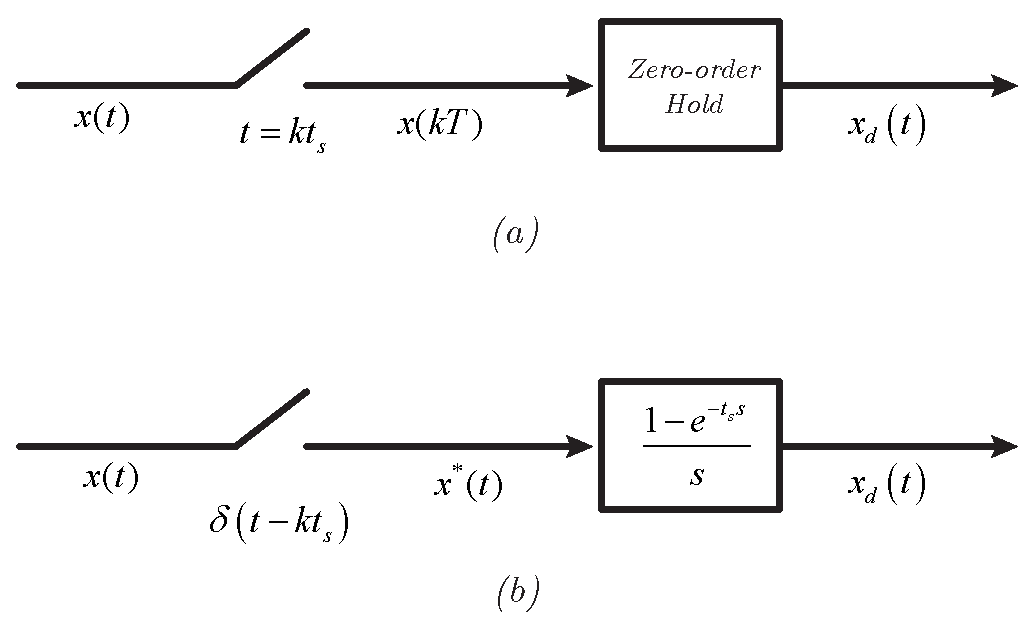
\includegraphics[width = 260pt, 
	keepaspectratio]{figures/discretization/sampling.eps}
	\captionsetup{width=0.5\textwidth, font=small}		
	\caption{(a) System with a sampler and zero order hold; (b) equivalent 
	system (mathematical model) which consists of an impulse sampler and 
	transfer function $(1-e^{-sT})/s$.}
	\label{figure_sampling}
\end{figure}
where 
\begin{equation}\label{discretization_eq_4}
	\begin{split}
		X^*(s) = \sum_{k=0}^{\infty} x(kt_s)e^{-kt_ss} 
	\end{split}
\end{equation}
\begin{mybox}
	The \textbf{transfer function of the zero-order hold} is given by
	\begin{equation}\label{discretization_eq_5}
		\begin{split}
			H_0(s) = \frac{1-e^{-t_ss}}{s}
		\end{split}
	\end{equation}
\end{mybox}
considering  the term $x(kt_s)$ constant in the equation 
Eq.~\ref{discretization_eq_4}, we obtain
\begin{equation}\label{discretization_eq_6}
	\begin{split}
		\mathcal{L}^{-1}\left[ X^*(s) \right] = x^*(t) = \sum_{k=-\infty}^{\infty}x(kt_s)\delta(t-kt_s)
	\end{split}
\end{equation}
Then,  the sampled signal $x^*(t)$ (in time domain) and the original continuous 
time signal $x(t)$ can be related as follows:
\begin{equation}\label{discretization_eq_7}
	\begin{split}
		x^*(t) &= ... + x(0)\delta(t)+x(t_s)\delta(t-t_s)+...+x(kt_s)\delta(t-kt_s)+...\\[6pt]
		&= \sum_{k=-\infty}^{\infty}x(kt_s)\delta(t-kt_s)
	\end{split}
\end{equation}
\noindent\textbf{The $\mathbf{\mathcal{Z}}$-transform}(Derivation). Consider 
the Laplace transform equation 
\begin{equation}\label{discretization_eq_8}
	\begin{split}
		X^*(s) = \sum_{k=0}^{\infty} x(kt_s)e^{-kt_ss} 
	\end{split}
\end{equation}
We define 
\begin{equation*}\label{discretization_eq_9}
	\begin{split}
		z=e^{t_ss} 
	\end{split}
\end{equation*}
or 
\begin{equation*}\label{discretization_eq_10}
	\begin{split}
		s=\frac{1}{t_s}\ln z 
	\end{split}
\end{equation*}
Then Eq. \ref{discretization_eq_8} becomes
\begin{equation}\label{discretization_eq_11}
	\begin{split}
		\left. X^*(s)\right|_{s=\frac{1}{t_s}\ln z }  = X(z) = 
		\sum_{k=0}^{\infty} x(kt_s)z^{-k} 
	\end{split}
\end{equation}

Note that the variable $z$ is a complex variable and $t_s$ is the sampling period. 

When we transform $e^{t_ss}$ to $z$, the concept of impulse sampling (which is 
purely a mathematical process) enables us to analyse by the 
$\mathcal{Z}$-transform method discrete time control systems which involve 
samplers and hold 
circuits. This means that by use the complex variable $z$, the techniques 
developed for the Laplace transform methods (such as the frequency response and 
root locus methods) can be readily applied to analyse discrete-time control 
systems involving sampling operations.

\begin{example}[\textbf{Obtain the $\mathcal{Z}$-transform of the Heaviside 
function $h(t)$}]
	
Define 
\begin{equation*}
	\begin{split}
		x(t) = h(t) 
	\end{split}
\end{equation*}
The impulse-sampled signal $x^*(t)$ can be obtained as follows:
\begin{equation*}
	\begin{split}
		x^*(t) = \sum_{k=0}^{\infty} x(kt_s)\delta(t-kt_s) = \sum_{k=0}^{\infty} \delta(t-kt_s)
	\end{split}
\end{equation*}
Then the Laplace transform of $x^*(t)$ can be given by
\begin{equation*}
	\begin{split}
		X^*(s) = \sum_{k=0}^{\infty} e^{-kt_ss} = \frac{1}{1-e^{-t_ss}}
	\end{split}
\end{equation*}
Note that $\sum_{k=0}^{\infty}x^{-k} = \frac{1}{1-x^{-1}}$ when $\abs{x}>1$.
Hence
\begin{equation*}
	\begin{split}
		X(z) = \mathcal{Z} \left[ h(t) \right] = \frac{1}{1-z^{-1}}
	\end{split}
\end{equation*}
$\triangleleft$
\end{example}

\begin{example}[\textbf{Obtain the $\mathcal{Z}$-transform of the sum of a 
generic function $x(t)$}]

Consider the function $x_d(kt_s)$ which is a sum of function $x(nt_s)$, where $n=0,1,2,...,k$, such that
\begin{equation*}
	\begin{split}
		x_d(kt_s) = \sum_{n=0}^{k}x(nt_s) \quad\quad k=0,1,2,...
	\end{split}
\end{equation*} 
where $x_d(kt_s)=0$ for $k<0$. Obtain the $\mathcal{Z}$ transform of $x_d(kt_s)$.

First not that
\begin{equation*}
	\begin{split}
		&x_d(kt_s) = x(0)+x(t_s)+...+x\left[(k-1)t_s\right]+x(kt_s) \\[6pt]
		&x_d\left[(k-1)t_s\right] = x(0)+x(t_s)+...+x\left[(k-1)t_s\right]
	\end{split}
\end{equation*} 
Hence 
\begin{equation*}
	\begin{split}
		x_d(kt_s) - x_d\left[(k-1)t_s\right] = x(kt_s) \quad\quad k=0,1,2,...
	\end{split}
\end{equation*} 
Therefore,
\begin{equation*}
	\begin{split}
		\mathcal{Z} \left[ x_d(kt_s) - x_d\left[(k-1)t_s\right] \right] = \mathcal{Z} \left[ x(kt_s) \right]
	\end{split}
\end{equation*}
or
\begin{equation*}
	\begin{split}
		X_d(z)-z^{-1}X_d(z) = X(z)
	\end{split}
\end{equation*}
which yields 
\begin{equation*}
	\begin{split}
		X_d(z) = \frac{1}{1-z^{-1}}X(z)
	\end{split}
\end{equation*}
or 
\begin{equation}\label{zsum}
	\begin{split}
		\mathcal{Z} \left[ \sum_{n=0}^{k}x(nt_s) \right] = \frac{1}{1-z^{-1}}X(z)
	\end{split}
\end{equation}
$\triangleleft$ \end{example}

\begin{example}\label{PIDinDTD}
\textbf{PID} control representation in discrete-time domain. The \textbf{PID} 
control in 
continuous time domain is given by:
\begin{equation}
	\begin{split}
		m(t) = k_p \ e(t) + k_i \int_{0}^{t} e(\tau)\ d\tau +k_d \ \dot{e}(t)
	\end{split}
\end{equation}
where $e(t)$ is the input to the controller.

In order to obtain the pulse transfer function for the digital \textbf{PID} 
controller, we may discretize the above equation. By approximating the integral 
term by the right Riemann summation and the derivative term by a two point 
difference form, we obtain:
\begin{figure}[H]
	\centering
	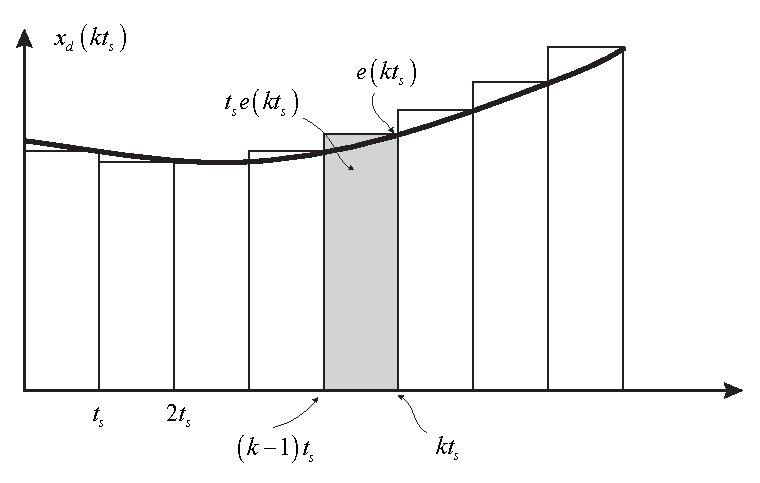
\includegraphics[width = 300pt, keepaspectratio]{figures/discretization/integration.eps}
		\captionsetup{width=0.5\textwidth, font=small}		
		\caption{Right Riemann Integration}
	\label{figure_discretization_2}
\end{figure}
\begin{equation}
	\begin{split}
		m(kt_s) = k_p \ e(kt_s) + k_i \ t_s \sum_{n=0}^{k} e(nt_s) + \frac{k_d}{t_s} \left\lbrace e(kt_s) - e\left[ (k-1)t_s\right] \right\rbrace  
	\end{split}
\end{equation}
Where the $\mathcal{Z}$-Transform of the integral term becomes, see Eq.~\eqref{zsum}
\begin{equation}
	\begin{split}
		\mathcal{Z}\left[\sum_{n=0}^{k} e(nt_s) \right] = \frac{1}{1-z^{-1}}E(z) 
	\end{split}
\end{equation}
\begin{mybox}
\textbf{	The pulse transfer function of the digital \textbf{PID} becomes}
	\begin{equation}
		\textbf{PID}(z) = \frac{M(z)}{E(z)} = k_p + t_s \frac{k_i}{1-z^{-1}} + 
		\frac{k_d}{t_s}(1-z^{-1})
	\end{equation}
Where in discrete time domain becomes $z^{-1} \rightarrow (k-1)$
\begin{equation}
	\begin{split}
		m(k) &= m_p(k) + m_i(k) + m_d(k)  \\[6pt]
		&\text{where} \\[6pt]
		m_p(k) &= k_p \ e(k) \\[6pt]
		m_i(k) &= m_i(k-1) + t_s \ k_i \ e(k) \\[6pt]
		m_d(k) &= \frac{k_d}{t_s} \left[e(k)-e(k-1) \right] 
	\end{split}
\end{equation}
\end{mybox}
$\triangleleft$ 
\end{example}

\subsection{Discrete-time Transform Methods}
It is common practice to design controller, filter, and general models in 
continuous time domain, and at the end of the design process, convert them into 
a discrete-time system using a discretization method. In the following, we are 
going to consider two different methods of discretization: \textit{backward 
difference method} and \textit{bilinear (or trapezoidal) transformation method}.

Shall be remembered that discretization of continuous time models, not only the particular method used, but also the sampling frequency chosen, will affect the dynamic characteristic of the resulting model. If the sampling frequency is sufficiently high, the equivalent discrete-time model will yield a good approximation to a given continuous time model.

\begin{example}(\textbf{Backward difference method.}) Digital Implementation of 
a Cruise Control. Consider the continuous time model
\begin{equation}\label{mainref}
	\begin{split}
		m\frac{dv(t)}{dt} + b v(t) = f(t)
	\end{split}
\end{equation}
or, where $b/m=\mu$ and $u(t)=f(t)/m$
\begin{equation}\label{mainref}
	\begin{split}
		\frac{dv(t)}{dt} + \mu v(t) = u(t)
	\end{split}
\end{equation}
where the Laplace transform is 
\begin{equation}\label{laplace_ref}
	\begin{split}
		\frac{V(s)}{U(s)} = \frac{1}{s+\mu}
	\end{split}
\end{equation}
and lets try to discretize with backward difference method:
Let us integrate both sides from $0$ to $t$:
\begin{equation}
	\begin{split}
		\int_{0}^{t}\frac{dv(t)}{dt} dt = - \mu \int_{0}^{t} v(t) dt + \int_{0}^{t} u(t) dt
	\end{split}
\end{equation}
\begin{figure}[H]
	\centering
	\includegraphics[width = 240pt, keepaspectratio]{figures/discretization/speed_model.eps}
			\captionsetup{width=0.5\textwidth, font=small}		
			\caption{Continuous time model.}
	\label{figure_model_speed}
\end{figure}
Substituting $t \rightarrow kt_s$ (we are in the $kt_s$ time step)
\begin{equation}
	\begin{split}
		\int_{0}^{kt_s}\frac{dv(t)}{dt} dt = - \mu \int_{0}^{kt_s} v(t) dt + \int_{0}^{kt_s} u(t) dt
	\end{split}
\end{equation}
which become
\begin{equation}\label{modeq1}
	\begin{split}
		v(kt_s)-v(0) = - \mu \int_{0}^{kv} v(t) dt + \int_{0}^{kv} u(t) dt
	\end{split}
\end{equation}
Consider now the time step $(k-1)t_s$ we obtain
\begin{equation}\label{modeq2}
	\begin{split}
		v\left[(k-1)t_s\right] -v(0) = - \mu \int_{0}^{(k-1)t_s} v(t) dt + \int_{0}^{(k-1)t_s} u(t) dt
	\end{split}
\end{equation}
By subtracting Eq.~\eqref{modeq2} from Eq~\eqref{modeq1} we obtain
\begin{equation}\label{modeq3}
	\begin{split}
		v(kt_s) - v\left[(k-1)t_s\right] = - \mu \int_{(k-1)t_s}^{kt_s} v(t) dt + \int_{(k-1)t_s}^{kt_s} u(t) dt
	\end{split}
\end{equation}
The integral term are now calculated by the backward difference method then
\begin{equation}
	\begin{split}
		\int_{(k-1)t_s}^{kt_s} v(t) dt = v(kt_s) \int_{(k-1)t_s}^{kt_s}  dt 
		=t_s v(kt_s)
	\end{split}
\end{equation}
and 
\begin{equation}
	\begin{split}
		\int_{(k-1)t_s}^{kt_s} u(t) dt =  u(kt_s) \int_{(k-1)t_s}^{kt_s} dt 
		=t_s u(kt_s)
	\end{split}
\end{equation}
Hence we obtain 
\begin{equation}\label{modeq4}
	\begin{split}
		v(kt_s) = v\left[(k-1)t_s\right] - \mu t_s v(kt_s) + t_s u(kt_s)
	\end{split}
\end{equation}
The $\mathcal{Z}$-Transform of Eq.~\eqref{modeq4} is 
\begin{equation}
	\begin{split}
		V(z) = V(z)z^{-1}-\mu t_s V(z) + t_s U(z)
	\end{split}
\end{equation}
for which we get
\begin{equation}
	\begin{split}
		\frac{V(z)}{U(z)} = \frac{1}{\frac{1-z^{-1}}{t_s}+\mu}
	\end{split}
\end{equation}
\begin{mybox}
	By comparing the $\mathcal{Z}$-transform with $\mathcal{L}$-transform 
	Eq.~\eqref{laplace_ref} we note that the right hand sides of these two 
	equations become identical if we let
	\begin{equation}\label{mapping}
		\begin{split}
			s = \frac{1-z^{-1}}{t_s}
		\end{split}
	\end{equation}
\end{mybox}

The Eq.~\eqref{mapping} is the mapping from the $s$ plane to the $z$ plane when the backward difference method is used to discretize Eq.~\eqref{mainref}.

The stability region in the $s$ plane, $\Big(\text{Re}(s)<0\Big)$, can be 
mapped by Eq. 
\ref{mapping} into the $z$ plane as follows.

Noting that the stable region in the $s$ plane is given by $\text{Re}(s)<0$, hence we can write
\begin{equation}
	\begin{split}
		\text{Re}\left(\frac{1-z^{-1}}{t_s} \right) &= \frac{1}{t_s}\text{Re}\left(\frac{z-1}{z} \right) = \\[6pt]
		&= \frac{1}{t_s}\text{Re}\left(\frac{\sigma +j\omega -1}{\sigma+j\omega} \right)<0
	\end{split}
\end{equation}
where
\begin{equation}
	\begin{split}
		& \text{Re} \left(\frac{\left( \sigma +j\omega -1 \right) \left(\sigma-j\omega \right) }{\left( \sigma+j\omega \right) \left(\sigma-j\omega \right) } \right) = \\[6pt]
		& = \text{Re} \left( \frac{\sigma^2-\sigma+\omega^2+j\omega}{\sigma^2+\omega^2}\right) = \\[6pt]
		& = \frac{\sigma^2-\sigma+\omega^2}{\sigma^2+\omega^2} <0
	\end{split}
\end{equation}
which can be written as
\begin{equation}
	\begin{split}
		\left( \sigma-\frac{1}{2} \right)^2+\omega^2 < \left( \frac{1}{2}\right)^2
	\end{split}
\end{equation}
The stable region can thus be mapped into a circle with center at $\sigma = 
\frac{1}{2}, \omega=0$ and radius equal to $\frac{1}{2}$ as shown in 
Figure~\ref{figure_discretization_3}. That mean the discretization method based 
on \textit{backward difference}, \textbf{transform a continuous-time stable 
system into a discrete-time stable system}.

\begin{figure}[H]
	\centering
	\includegraphics[width = 380pt, 
	keepaspectratio]{figures/discretization/backward.eps}
		\captionsetup{width=0.5\textwidth, font=small}		
		\caption{Mapping of the left half of the s plane into z plane by $s = (1-z^{-1})/t_s$ (backward difference method).}
	\label{figure_discretization_3}
\end{figure}
$\triangleleft$ 
\end{example}

\begin{example}(\textbf{Bilinear transformation method.})
the bilinear transformation method is also called the trapezoidal integration 
method or Tustin transformation method. By this method we approximate the areas 
\begin{equation*}\label{tustin_eq_1}
	\begin{aligned}
		\int_{(k-1)t_s}^{kt_s}x_d(t)dt
	\end{aligned}\quad\text{and}\quad
	\begin{aligned}
	\int_{(k-1)t_s}^{kt_s}x(t)dt
\end{aligned}
\end{equation*}
by $\frac{1}{2}\big[x_d(kt_s) - x_d((k-1)t_s)\big]t_s$ and 
$\frac{1}{2}\big[x(kt_s) - x((k-1)t_s)\big]t_s$, respectively; Notice that the 
integration scheme assumes that the variation between successive sampling 
points is linear, as shown in Figure~\ref{figure_discretization_4}. Hence by 
the use of the bilinear transformation method, Eq.~\eqref{modeq4} can be 
written as follows:
\begin{equation}\label{tustin_eq_2}
	\begin{aligned}
	v(kt_s)=v[(k-1)t_s]-&\mu\frac{t_s}{2}\big[v(kt_s) + 
		v((k-1)t_s)\big] + \\[6pt]
		&+\frac{t_s}{2}\big[u(kt_s) + u((k-1)t_s)\big]
	\end{aligned}
\end{equation}
The $\mathcal{Z}$-transform of Eq,~\eqref{tustin_eq_2} is
\begin{equation}\label{tustin_eq_3}
	\begin{aligned}
		V(z)=z^{-1}V(z)-&\mu\frac{t_s}{2}\Big[V(z)+z^{-1}V(z)\Big]+ 
		\\[6pt]
		&+\frac{t_s}{2}\Big[U(z)+z^{-1}U(z)\Big]
	\end{aligned}
\end{equation}
\begin{figure}[H]
	\centering
	\includegraphics[width = 280pt, 
	keepaspectratio]{figures/discretization/bilinear_integration.eps}
	\captionsetup{width=0.5\textwidth, font=small}		
	\caption{Area approximation bt the bilinear transformation method (also 
	called Tustin).}
	\label{figure_discretization_4}
\end{figure}
for which we get
\begin{equation}\label{tustin_eq_4}
	\begin{split}
		\frac{V(z)}{U(z)} = \frac{1}{\frac{2}{t_s}\frac{1-z^{-1}}{1+z^{-1}}+\mu}
	\end{split}
\end{equation}
\begin{mybox}
	By comparing the $\mathcal{Z}$-transform with $\mathcal{L}$-transform 
	Eq.~\eqref{tustin_eq_4} we note that the right hand sides of these two 
	equations become identical if we let
	\begin{equation}\label{tustin_eq_5}
		\begin{split}
			s = \frac{2}{t_s}\frac{1-z^{-1}}{1+z^{-1}}
		\end{split}
	\end{equation}
	The Eq.~\eqref{tustin_eq_5} is the mapping from the $s$ plane to the $z$ 
	plane when the bilinear transformation method is used to discretize 
	Eq.~\eqref{mainref}.
\end{mybox}

The stability region in the $s$ plane can be mapped by Eq.~\eqref{tustin_eq_5} into the $z$ plane as follows.

Noting that the stable region in the $s$ plane is given by $\text{Re}(s)<0$, hence we can write
\begin{equation}\label{tustin_eq_6}
	\begin{split}
		\text{Re}\left(\frac{2}{t_s}\frac{1-z^{-1}}{1+z^{-1}} \right) &= \frac{2}{t_s}\text{Re}\left(\frac{z-1}{z+1} \right) = \\[6pt]
		&= \frac{2}{t_s}\text{Re}\left(\frac{\sigma -1 +j\omega}{\sigma+1+j\omega} \right)<0
	\end{split}
\end{equation}
where
\begin{equation}\label{tustin_eq_7}
	\begin{split}
		& \text{Re}\left(\frac{\sigma -1 +j\omega}{\sigma+1+j\omega} \right) = \\[6pt]
		& = \frac{\sigma^2-1+\omega^2}{(\sigma+1)^2+\omega^2} <0
	\end{split}
\end{equation}
Eq.~\eqref{tustin_eq_7} is hold when
\begin{equation}\label{tustin_eq_8}
	\begin{split}
		\sigma^2+\omega^2 < 1
	\end{split}
\end{equation}
The stable region can thus be mapped into a circle with center at $\sigma = 0, \omega=0$ and radius equal to $1$ as shown in Figure~\ref{figure_discretization_5}
\begin{figure}[H]
	\centering
	\includegraphics[width = 380pt, 
	keepaspectratio]{figures/discretization/bilinear_mapping.eps}
	\captionsetup{width=0.5\textwidth, font=small}		
	\caption{Mapping of the left half of the s plane into z plane by $s = 
	2/t_s(1-z^{-1})/(1+z^{-1})$ (bilinear transformation method).}
	\label{figure_discretization_5}
\end{figure}
That mean the discretization method based on \textit{Tustin}, \textbf{transform 
a continuous-time stable system into a discrete-time stable system}.
$\triangleleft$ 
\end{example}


\section{Discrete-time Representation of State Space}
Up to now we have seen system represented in the contest of continuous time 
domain where they are described by differential equation. Any continuous-time 
dynamical system can be rewritten in the form of discrete-time domain. This 
process is called \textit{discretization of continuous-time systems}. The 
discretized system is always an approximation of the continuous-time case.

Consider the continuous-time domain representation of 
Eq.~\eqref{ss_realization_dt_eq1}
\begin{equation}\label{ss_realization_dt_eq1}
	\Bigg\{ 	\begin{aligned}
		\dot{\vec{x}}(t)  &= \tilde{\mathbf{A}} \,\vec{x}(t) +\tilde{\mathbf{B}} \,u(t), \quad\vec{x}(0)=\vec{x}_0 \\[6pt]
		\vec{y}(t)  &= {\mathbf{C}} \,\vec{x}(t)
	\end{aligned}
\end{equation}
and the equivalent discrete-time domain representation of 
Eq.~\eqref{ss_realization_dt_eq2}
\begin{equation}\label{ss_realization_dt_eq2}
	\Bigg\{ 	\begin{aligned}
		\vec{x}(k+1) & = \mathbf{A}\vec{x}(k) + \mathbf{B}\vec{u}(k),\quad\vec{x}(0)=\vec{x}_0 \\[6pt]
		\vec{y}(k) & = \mathbf{C}\vec{x}(k)
	\end{aligned}
\end{equation}
they represent the same dynamical system. As we can see the two transition 
matrices $\tilde{\mathbf{A}}$ and $\mathbf{A}$ as well as the two input matrices
$\tilde{\mathbf{B}}$ and $\mathbf{B}$ are different.

Exist a transformation method which, for a given discrete time step, correlates matrix $\tilde{\mathbf{A}}$ to matrix $\mathbf{A}$ and matrix $\tilde{\mathbf{B}}$ to matrix $\mathbf{B}$.
\begin{figure}[H]
	\centering
	\begin{subfigure}{.75\textwidth}
		\centering
		\includegraphics[width = 0.75\textwidth, width = 325pt, keepaspectratio]{figures/ct_state_space_rep_1.eps}
		\captionsetup{width=0.5\textwidth, font=small}		
		\caption{Block diagram of the linear time-invariant continuous-time system represented in state space.}
		\label{ct_ref}
	\end{subfigure}
	\begin{subfigure}{.75\textwidth}
		\centering
		\includegraphics[width = 0.75\textwidth, width = 325pt, keepaspectratio]{figures/dt_state_space_rep_1.eps}
		\captionsetup{width=0.5\textwidth, font=small}		
		\caption{Block diagram of the linear time-invariant discrete-time system represented in state space.}
		\label{dt_ref}
	\end{subfigure}
	\captionsetup{width=0.5\textwidth, font=small}		
	\caption{State space representation of a given dynamical system in both continuous and discrete-time domain.}
	\label{ss_rep}
\end{figure}

Before to derive the relation between $\tilde{\mathbf{A}}$ and $\mathbf{A}$, 
and between $\tilde{\mathbf{B}}$ and $\mathbf{B}$, we present some relevant and 
propaedeutic results for discrete time state space representation.

As shown for the continuous time case, we now present the solution for the 
discrete-time case, namely we present the solution of the system of 
Eq.~\eqref{ss_realization_dt_eq2}
\begin{equation}\label{ss_realization_dt_eq3}
	\vec{x}(k+1) = \mathbf{A}\vec{x}(k) + \mathbf{B}u(k)
\end{equation}
by a recursion procedure and then by the $z$ transform method. Them we discuss 
methods for computing $(z\mathbf{I}-\mathbf{A})^{-1}$.

In general, discrete-time equation are easier to solve than differential 
equations because the former can be solved easily by means of recursion 
procedure. The recursion procedure is quite simple and convenient for digital 
computations.

\subsection{Solutions of the Non Homogeneous State Space Equation in 
	Discrete-time Domain}
Consider the following state equation and output equation:
\begin{equation}\label{ss_solution_dt_eq1}
\begin{aligned}
		\vec{x}(k+1) &= \mathbf{A}\vec{x}(k) + \mathbf{B}\vec{u}(k) \\[6pt]
%		\vec{y}(k) &= \mathbf{C}\vec{x}(k)
	\end{aligned}
\end{equation}
\begin{equation}\label{ss_solution_dt_eq1b}
\begin{aligned}
%		\vec{x}(k+1) &= \mathbf{A}\vec{x}(k) + \mathbf{B}\vec{u}(k) \\[6pt]
		\vec{y}(k) &= \mathbf{C}\vec{x}(k)
	\end{aligned}
\end{equation}
The solution, for any positive integer, may be obtained directly by recursion, 
as follows:
\begin{equation}\label{ss_solution_dt_eq2}
	\begin{aligned}
		\vec{x}(1) &= \mathbf{A}\vec{x}(0) + \mathbf{B}\vec{u}(0)\\[6pt]
		\vec{x}(2) &= \mathbf{A}\vec{x}(1) + \mathbf{B}\vec{u}(1) = 
		\mathbf{A}^2\vec{x}(0) + 
		\mathbf{A}\mathbf{B}\vec{u}(0)+\mathbf{B}\vec{u}(1)\\[6pt]
		\vec{x}(3) &= \mathbf{A}\vec{x}(2) + \mathbf{B}\vec{u}(2) = 
		\mathbf{A}^3\vec{x}(0) + 
		\mathbf{A}^2\mathbf{B}\vec{u}(0)+\mathbf{A}\mathbf{B}\vec{u}(1)+\mathbf{B}\vec{u}(2)\\[6pt]
		&\vdots
	\end{aligned}
\end{equation}
\begin{mybox}
	By repeating this procedure, we obtain the solution of 
	Eq.~\eqref{ss_solution_dt_eq1}
	\begin{equation}\label{ss_solution_dt_eq3}
		\begin{aligned}
			\vec{x}(k) = \mathbf{A}^k\vec{x}(0) + 
			\sum_{j=0}^{k-1}\mathbf{A}^{k-j-1}\mathbf{B}\vec{u}(j) \quad \quad 
			k=1,2,3,...
		\end{aligned}
	\end{equation}
\end{mybox}

Clearly, $\vec{x}(k)$ consists of two parts, one representing the contribution 
of the initial state $\vec{x}(0)$, and the other the contribution of the input 
$\vec{u}(j)$, where $j = 0,1,2,...,k-1$. The output $\vec{y}(k)$ is given by
\begin{equation}\label{ss_solution_dt_eq4}
	\begin{aligned}
		\vec{y}(k) = \mathbf{C}\mathbf{A}^k\vec{x}(0) + 
		\mathbf{C}\sum_{j=0}^{k-1}\mathbf{A}^{k-j-1}\mathbf{B}\vec{u}(j)
	\end{aligned}
\end{equation}
Notice that it is possible to write the solution of the homogeneous state 
equation
\begin{equation}\label{ss_solution_dt_eq5}
	\begin{aligned}
		\vec{x}(k+1) = \mathbf{A}\vec{x}(k)
	\end{aligned}
\end{equation}
as 
\begin{equation}\label{ss_solution_dt_eq6}
	\begin{aligned}
		\vec{x}(k) = \mathbf{\Psi}(k)\vec{x}(0)
	\end{aligned}
\end{equation}
where $\mathbf{\Psi}(k)$ is a unique $n \times n$ matrix satisfying the 
condition
\begin{equation}\label{ss_solution_dt_eq7}
	\begin{aligned}
		\mathbf{\Psi}(k+1) = \mathbf{A}\mathbf{\Psi}(k) \quad \quad 
		\mathbf{\Psi}(0)=\mathbf{I}
	\end{aligned}
\end{equation}
Clearly, $\mathbf{\Psi}(k)$ can be given by 
\begin{equation}\label{ss_solution_dt_eq8}
	\begin{aligned}
		\mathbf{\Psi}(k) = \mathbf{A}^k
	\end{aligned}
\end{equation}
From Eq.~\eqref{ss_solution_dt_eq8}, we see that the solution of 
Eq.~\eqref{ss_solution_dt_eq5} is simply a 
transformation of the initial state. Therefore, the unique matrix 
$\mathbf{\Psi}(k)$ is called the \textit{state transition matrix}. It is also 
called the \textit{the fundamental matrix}. The state transition matrix 
contains all the information about the free motions of the system define by 
Eq.~\eqref{ss_solution_dt_eq5}.

In terms of the state transition matrix $\mathbf{\Psi}(k)$, Eq. 
\ref{ss_solution_dt_eq3} can be 
written in the form
\begin{equation}\label{ss_solution_dt_eq9}
	\begin{aligned}
		\vec{x}(k) &= 
		\mathbf{\Psi}(k)\vec{x}(0)+\sum_{j=0}^{k-1}\mathbf{\Psi}(k-j-1)\mathbf{B}\vec{u}(j)
		 \\[6pt]
		&=\mathbf{\Psi}(k)\vec{x}(0)+\sum_{j=0}^{k-1}\mathbf{\Psi}(j)\mathbf{B}\vec{u}(k-j-1)
	\end{aligned}
\end{equation}
Substituting Eq.~\eqref{ss_solution_dt_eq9} into second equation of 
Eq.~\eqref{ss_solution_dt_eq1}, we obtain:
\begin{equation}\label{ss_solution_dt_eq10}
	\begin{aligned}
		\vec{y}(k) &= 
		\mathbf{C}\mathbf{\Psi}(k)\vec{x}(0)+\mathbf{C}\sum_{j=0}^{k-1}\mathbf{\Psi}(j)\mathbf{B}\vec{u}(k-j-1)
	\end{aligned}
\end{equation}

\subsection{$\mathbf{\mathcal{Z}}$-Transform Approach to the Solution of 
	Discrete-time State Equations.} We now present the solution of 
	discrete-time 
state 
equation 
by the $\mathcal{Z}$-transform method. Consider the discrete-time system 
described by 
Eq.~\eqref{zt_approach_1}:
\begin{equation}\label{zt_approach_1}
	\begin{aligned}
		\vec{x}(k+1) &= \mathbf{A}\vec{x}(k)+\mathbf{B}\vec{u}(k)
	\end{aligned}
\end{equation}
Taking the $\mathcal{Z}$-transform of both sides of Eq.~\eqref{zt_approach_1} 
gives
\begin{equation}\label{zt_approach_2}
	\begin{aligned}
		z{\vec{X}}(z) -z\vec{x}(0) &= 
		\mathbf{A}{\vec{X}}(z)+\mathbf{B}{\vec{U}}(z)
	\end{aligned}
\end{equation}
where ${\vec{X}}(z) = \mathcal{Z}\left[ \vec{x}(k)\right]$ and ${\vec{U}}(z) 
= \mathcal{Z}\left[ \vec{u}(k)\right]$. Then
\begin{equation}\label{zt_approach_3}
	\begin{aligned}
		\left( z\mathbf{I}-\mathbf{A}\right){\vec{X}}(z) = z\vec{x}(0) + 
		\mathbf{B}{\vec{U}}(z)
	\end{aligned}
\end{equation}
Premultiplying both sides of this last equation by $\left( 
z\mathbf{I}-\mathbf{A}\right)^{-1}$, we obtain 
\begin{equation}\label{zt_approach_4}
	\begin{aligned}
		{\vec{X}}(z) = \left( z\mathbf{I}-\mathbf{A}\right)^{-1}z 
		\vec{x}(0)+\left( 
		z\mathbf{I}-\mathbf{A}\right)^{-1}\mathbf{B}{\vec{U}}(z)
	\end{aligned}
\end{equation}
Taking the inverse $\mathcal{Z}$-transform ($\mathcal{Z}^{-1}$) of both sides 
of Eq.~\eqref{zt_approach_4} gives
\begin{equation}\label{zt_approach_5}
	\begin{aligned}
		\vec{x}(k) = \mathcal{Z}^{-1}\left[ \left( 
		z\mathbf{I}-\mathbf{A}\right)^{-1}z\right] 
		\vec{x}(0)+\mathcal{Z}^{-1}\left[ \left( 
		z\mathbf{I}-\mathbf{A}\right)^{-1}\mathbf{B}{\vec{U}}(z)\right] 
	\end{aligned}
\end{equation}
Comparing Eq.~\eqref{ss_solution_dt_eq3} with  Eq.~\eqref{zt_approach_5}, we 
obtain 
\begin{equation}\label{zt_approach_6}
	\begin{aligned}
		\mathbf{A}^k=\mathcal{Z}^{-1}\left[ \left( 
		z\mathbf{I}-\mathbf{A}\right)^{-1}z \right] 
	\end{aligned}
\end{equation}
and
\begin{equation}\label{zt_approach_7}
	\begin{aligned}
		\sum_{j=0}^{k-1}\mathbf{A}^{k-j-1}\mathbf{B}\vec{u}(j)=\mathcal{Z}^{-1}\left[
		\left( z\mathbf{I}-\mathbf{A}\right)^{-1}\mathbf{B}{\vec{U}}(z) 
		\right] 
	\end{aligned}
\end{equation}
where $k=1,2,3,...$

Notice that the solution by the $z$ transform method involves the process of 
the inverting the matrix $ \left( z\mathbf{I}-\mathbf{A}\right)$, accomplished 
by analytical means or by use of a computer routine. The solution also requires 
the inverse $\mathcal{Z}$-transform of $ \left( 
z\mathbf{I}-\mathbf{A}\right)^{-1}z$ and 
$\left( z\mathbf{I}-\mathbf{A}\right)^{-1}\mathbf{B}{\vec{U}}(z)$.


\subsection{Non-Uniqueness of State Space Representation.} For a given 
pulse-transfer-function system the state space representation is not unique. We 
have demonstrated that different state space representation for a given 
pulse-transfer-function system are possible. The state equation, however, are 
related to each other by the similarity transformation.

Consider the  system defined by
\begin{equation}\label{nu_eq1}
	\left\lbrace \begin{aligned}
		\vec{x}(k+1) & = \mathbf{A}\vec{x}(k) + \mathbf{B}\vec{u}(k) \\[6pt]
		\vec{y}(k) & = \mathbf{C}\vec{x}
	\end{aligned}\right. 
\end{equation}
Let us define a new state vector ${\vec{z}}$ by
\begin{equation}\label{nu_eq2}
	{\vec{x}}(k) = \mathbf{T}{\vec{z}}(k)
\end{equation}
where $\mathbf{T}$ is a non-singular matrix. Then by substituting Eq. 
(\ref{nu_eq2}) into (\ref{nu_eq1}) we obtain
\begin{equation}\label{nu_eq3}
	\mathbf{T}{\vec{z}}(k+1) = \mathbf{A}\mathbf{T}{\vec{z}}(k)+ 
	\mathbf{B}\vec{u}(k)
\end{equation}
Left-multiplying both sides by $\mathbf{T}^{-1}$ yields
\begin{equation}\label{nu_eq4}
	{\vec{z}}(k+1) = \mathbf{T}^{-1}\mathbf{A}\mathbf{T}{\vec{z}}(k)+ 
	\mathbf{T}^{-1}\mathbf{B}\vec{u}(k)
\end{equation}
Let us define
\begin{equation*}\label{nu_eq5}
	\mathbf{T}^{-1}\mathbf{A}\mathbf{T} = {\mathbf{G}}, \quad 
	\mathbf{T}^{-1}\mathbf{B} = {\mathbf{H}}
\end{equation*}
Then Eq.~\eqref{nu_eq1} can be written as follows:
\begin{equation}\label{nu_eq6}
	{\vec{z}}(k+1) = {\mathbf{G}}{\vec{z}}(k)+ {\mathbf{H}}\vec{u}(k)
\end{equation}
By defining 
\begin{equation*}\label{nu_eq7}
	\mathbf{C}\mathbf{T} = {\mathbf{M}}
\end{equation*}
we can write:
\begin{equation}\label{nu_eq8}
	\begin{aligned}
		{\vec{y}}(k) & = \mathbf{M}{\vec{z}}
	\end{aligned}
\end{equation}
We have thus shown that the state space representation given by 
Eq.~\eqref{nu_eq1} is equivalent to the state representation given by 
Eq.~\eqref{nu_eq6} and Eq.~\eqref{nu_eq8}
\begin{equation}\label{nu_eq9}
	\left\{\begin{aligned}
		\vec{x}(k+1) & = \mathbf{A}\vec{x}(k) + \mathbf{B}\vec{u}(k) \\[6pt]
		\vec{y}(k) & = \mathbf{C}\vec{x}
	\end{aligned}\right. \iff
	\left\{\begin{aligned}
		{\vec{z}}(k+1) & = {\mathbf{G}}{\vec{z}}(k) + {\mathbf{H}}{\vec{u}}(k) 
		\\[6pt]
		\vec{y}(k) & = {\mathbf{M}}{\vec{z}}
	\end{aligned}\right.
\end{equation}

\section{Canonical State Space Representation}
\begin{mybox}
There are many techniques available for obtaining state space representations 
of discrete-time systems. Consider the discrete-time system described by the 
following ARMA model
\begin{equation}\label{canonical_ss_representation_eq_1}
	\begin{aligned}
		y(k) &+ a_{n-1}y(k-1)+a_{n-2}y(k-2)+\cdots+a_0y(k-n) = \\[6pt]
		&= b_nu(k)+b_{n-1}u(k-1)+\cdots+b_0u(k-n) \\
	\end{aligned}
\end{equation}
where $u(k)$ is the input and $y(k)$ is the output of the system at the $k$th sampling instant. Note that some of the coefficients $a_i$ $(i=1,2,\cdots,n)$ and $b_j$ $(j=1,2,\cdots,n)$ may be zero. Eq.~\ref{canonical_ss_representation_eq_1} can be written in the form of the pulse transfer function as
\begin{equation}\label{canonical_ss_representation_eq_2}
	\begin{aligned}
		G(z)=\frac{Y(z)}{U(z)} &= \frac{b_nz^n+b_{n-1}z^{n-1}+ \cdots +b_1z+b_0}{z^n+a_{n-1}z^{n-1}+ \cdots +a_1z+a_0}
	\end{aligned}
\end{equation}
or 
\begin{equation}\label{canonical_ss_representation_eq_3}
	\begin{aligned}
		G(z)=\frac{Y(z)}{U(z)} = \frac{b_n +b_{n-1}z^{-1}+ \cdots +b_1 z^{-(n-1)} + b_0 z^{-n}}{1 + a_{n-1}z^{-1}+ \cdots +a_1 z^{-(n-1)}+a_0 z^{-n}}
	\end{aligned}
\end{equation}
\end{mybox}
\subsection{Controllable Canonical Form.} \begin{mybox} The state space 
representation of the 
transfer function system given by Eq.~\eqref{canonical_ss_representation_eq_1} 
in the controllable canonical 
form is given by the following equations:
\begin{equation}\label{ccanonical_form_eq1}
	\mathbf{A} = \left[ \begin{matrix}
		0 & 1 & 0 & \cdots & 0 \\
		0 & 0 & 1 & \cdots & 0 \\
		\vdots & \vdots & \vdots &  & \vdots \\
		0 & 0 & 0 & \cdots & 1 \\
		-a_0 & -a_1 & -a_2 & \cdots & -a_{n-1} \\
	\end{matrix}\right] 
\end{equation}

\begin{equation}\label{ccanonical_form_eq2}
	\mathbf{B} = \left[ \begin{matrix}
		0  \\
		0  \\
		\vdots \\
		0  \\
		1  \\
	\end{matrix}\right] 
\end{equation}

\begin{equation}\label{ccanonical_form_eq3}
	\mathbf{C} = \left[ \begin{matrix}
		b_0-a_0b_n, & b_1-a_1b_n, & \cdots, & b_{n-1}-a_{n-1}b_n
	\end{matrix}\right] 
\end{equation}

\begin{equation}\label{ccanonical_form_eq4}
	\mathbf{D} = b_n 
\end{equation}
\end{mybox}


\subsection{Partial-Fraction-Expansion Programming Method.} The programming 
method using partial fraction expansion applies when the denominator of the 
pulse transfer function is in a factored form.
Consider the system defined by
\begin{equation}\label{pfepm_eq_1}
	\begin{aligned}
		G(z)&=\frac{Y(z)}{U(z)} = \frac{b_nz^n+b_{n-1}z^{n-1}+ \cdots +b_1z+b_0}{z^n+a_{n-1}z^{n-1}+ \cdots +a_1z+a_0} = \\[6pt]
		&= b_n+\frac{(b_{n-1}-a_{n-1}b_n)z^{n-1}+(b_{n-2}-a_{n-2}b_n)z^{n-2}+\cdots+(b_0-a_0b_n)}{(z-p_{n-1})(z-p_{n-2})\cdots(z-p_{0})}
	\end{aligned}
\end{equation}
we shall first discuss the case where all poles are distinct. Then we shall consider the case where multiple poles are involved.

\vspace{5mm}
\noindent\textbf{\textit{Case 1: $\mathbf{G(z)}$ Involves Distinct Poles Only.}} In this case Eq.~\eqref{pfepm_eq_1} can be expanded into partial fractions as follows:
\begin{equation}\label{pfepm_eq_2}
	\begin{aligned}
		G(z)=\frac{Y(z)}{U(z)} = b_n + \frac{c_{n-1}}{z-p_{n-1}}+\frac{c_{n-2}}{z-p_{n-2}}+\cdots+\frac{c_0}{z-p_0}
	\end{aligned}
\end{equation}
where
\begin{equation}\label{pfepm_eq_3}
	\begin{aligned}
		c_i = \lim_{z \to p_i} \left[\frac{Y(z)}{X(z)}(z-p_i)\right]
	\end{aligned}
\end{equation}
Equation (\ref{}) can be written in the form 
\begin{equation}\label{pfepm_eq_4}
	\begin{aligned}
		Y(z)= b_n U(z) + \frac{c_{n-1}}{z-p_{n-1}}U(z)+\frac{c_{n-2}}{z-p_{n-2}}U(z)+\cdots+\frac{c_0}{z-p_0}U(z)
	\end{aligned}
\end{equation}
Let us define the state variables as follows:
\begin{equation}\label{pfepm_eq_5}
	\begin{aligned}
		X_1(z)= & \enspace  \frac{1}{z-p_1}U(z) \\[6pt]
		X_2(z)= & \enspace  \frac{1}{z-p_2}U(z) \\[6pt]
		X_3(z)= & \enspace  \frac{1}{z-p_3}U(z) \\[6pt]
		& \enspace \vdots \\[6pt]
		X_n(z)= & \enspace  \frac{1}{z-p_n}U(z) 
	\end{aligned}
\end{equation}
then can be rewritten as
\begin{equation}\label{pfepm_eq_6}
	\begin{aligned}
		zX_1(z)= & \enspace  p_1X_1+U(z) \\[6pt]
		zX_2(z)= & \enspace  p_2X_2+U(z) \\[6pt]
		& \enspace \vdots \\[6pt]
		zX_n(z)= & \enspace  p_nX_n+U(z) \\[6pt]
	\end{aligned}
\end{equation}
Also, Eq.~\eqref{pfepm_eq_4} can be written as
\begin{equation}\label{pfepm_eq_7}
	\begin{aligned}
		Y(z)= b_n U(z) + c_1X_1(z)+ c_2X_2(z)+ \cdots +c_nX_n(z)
	\end{aligned}
\end{equation}
The inverse $\mathcal{Z}$ transformation of Eqs.~\eqref{pfepm_eq_6}) 
and~\eqref{pfepm_eq_7} gives
\begin{equation}\label{pfepm_eq_8}
	\begin{aligned}
		x_1(k+1) =& \enspace p_1x_1(k)+u(k) \\[6pt]
		x_2(k+1) =& \enspace p_2x_2(k)+u(k) \\[6pt]
		& \enspace\vdots \\[6pt]
		x_n(k+1) =& \enspace p_nx_n(k)+u(k) \\[6pt]
	\end{aligned}
\end{equation}
and
\begin{equation}\label{pfepm_eq_9}
	\begin{aligned}
		y(k) = c_1x_1(k)+c_2x_2(k)+\cdots+c_nx_n(k)+b_0u(k)
	\end{aligned}
\end{equation}

Rewriting the state equation and the output equation in the form of 
vector-matrix equations, we obtain
\begin{equation}\label{pfepm_eq_10}
	\left[\begin{matrix}
		x_1(k+1) \\
		x_2(k+1) \\
		\vdots \\
		x_n(k+1)
	\end{matrix}\right] = 
	\left[\begin{matrix}
		p_1 & 0 & \cdots & 0 \\
		0 & p_2 & \cdots & 0 \\
		\vdots & \vdots & & \vdots\\
		0 & 0 & \cdots & p_n \\
	\end{matrix}\right]
	\left[\begin{matrix}
		x_1(k) \\
		x_2(k) \\
		\vdots \\
		x_n(k)
	\end{matrix}\right] + 
	\left[\begin{matrix}
		1 \\
		1 \\
		\vdots \\
		1
	\end{matrix}\right] u(k)
\end{equation}
and
\begin{equation}\label{pfepm_eq_11}
	y(k) = 
	\left[\begin{matrix}
		c_1 & c_2 & \cdots & c_n \\
	\end{matrix}\right] 
	\left[\begin{matrix}
		x_1(k) \\
		x_2(k) \\
		\vdots \\
		x_n(k)
	\end{matrix}\right] + b_0 u(k)
\end{equation}
Notice that the $n \times n$ state matrix is diagonal matrix. The diagonal 
elements are the poles of $G(z) = {Y(z)}/{X(z)}$.

\vspace{5mm}
\noindent\textbf{\textit{Case 2: $\mathbf{G(z)}$ Involves Multiple Poles.}}
In the discussion that follows, we assume that $G(z)$ involves a multiple pole of order $m$ at $z=p_1$ and that all other poles are distinct.
Consider the system defined by Eq.~\eqref{pfepm_eq_1}. Since $G(z)$ can be 
written in the form 
\begin{equation}\label{pfepm_eq_12}
	\begin{aligned}
		G(z)&=\frac{Y(z)}{U(z)} = \frac{b_nz^n+b_{n-1}z^{n-1}+ \cdots +b_1z+b_0}{(z-p_1)^m(z-p_{m+1})(z-p_{m+2})\cdots(z-p_n)} = \\[8pt]
		&= b_n+\frac{(b_{n-1}-a_{n-1}b_n)z^{n-1}+(b_{n-2}-a_{n-2}b_n)z^{n-2}+\cdots+(b_0-a_0b_n)}{(z-p_1)^m(z-p_{m+1})(z-p_{m+2})\cdots(z-p_n)} = \\[8pt]
		&= b_n + \frac{c_1}{(z-p_1)^m}+\frac{c_2}{(z-p_2)^{m-1}}+\cdots+\frac{c_m}{z-p_1}+ \\[8pt]
		& \quad \quad \enspace + \frac{c_{m+1}}{z-p_{m+1}} +\frac{c_{m+2}}{z-p_{m+2}}+\cdots+\frac{c_{n}}{z-p_{n}}
	\end{aligned}
\end{equation}
we obtain 
\begin{equation}\label{pfepm_eq_13}
	\begin{aligned}
		Y(z) &= b_n U(z) + \frac{c_{1}}{(z-p_{1})^m}U(z)+\frac{c_{2}}{(z-p_{2})^{m-1}}U(z)+\cdots+\frac{c_m}{z-p_1}U(z) \\[6pt] 
		& +\frac{c_{m+1}}{z-p_{m+1}}U(z) +\frac{c_{m+2}}{z-p_{m+2}}U(z) + \cdots +\frac{c_{n}}{z-p_{n}}U(z)
	\end{aligned}
\end{equation}
Let us define the first $m$ state variables $X_1(z), X_2(z),\cdots,X_m(z)$ by the equations:
\begin{equation}\label{pfepm_eq_14}
	\begin{aligned}
		X_1(z)= & \enspace  \frac{1}{(z-p_1)^m}U(z) \\[6pt]
		X_2(z)= & \enspace  \frac{1}{(z-p_1)^{m-1}}U(z) \\[6pt]
		X_3(z)= & \enspace  \frac{1}{(z-p_1)^{m-2}}U(z) \\[6pt]
		& \enspace \vdots \\[6pt]
		X_m(z)= & \enspace  \frac{1}{z-p_1}U(z) 
	\end{aligned}
\end{equation}
and the remaining $n-m$ state variables $X_{m+1}(z),X_{m+2}(z),\cdots,X_n(z)$ by the equations
\begin{equation}\label{pfepm_eq_15}
	\begin{aligned}
		X_{m+1}(z)= & \enspace  \frac{1}{z-p_{m+1}}U(z) \\[6pt]
		X_{m+2}(z)= & \enspace  \frac{1}{z-p_{m+2}}U(z) \\[6pt]
		X_{m+3}(z)= & \enspace  \frac{1}{z-p_{m+3}}U(z) \\[6pt]
		& \enspace \vdots \\[6pt]
		X_n(z)= & \enspace  \frac{1}{z-p_n}U(z) 
	\end{aligned}
\end{equation}
Notice that the $m$ state variables defined by Eq.~\eqref{pfepm_eq_15} are 
related each to the next by the following equations:
\begin{equation}\label{pfepm_eq_16}
	\begin{aligned}
		\frac{X_{1}(z)}{X_2(z)}= & \enspace  \frac{1}{z-p_{1}} \\[6pt]
		\frac{X_{2}(z)}{X_3(z)}= & \enspace  \frac{1}{z-p_{1}} \\[6pt]
		& \enspace \vdots \\[6pt]
		\frac{X_{m-1}(z)}{X_m(z)}= & \enspace  \frac{1}{z-p_{1}} \\[6pt]
	\end{aligned}
\end{equation}
By taking the inverse $\mathcal{Z}$ transforms of all of Eq. (\ref{}), the 
last equation in Eq. (\ref{}), and all of Eq. (\ref{}), we obtain
\begin{equation}\label{pfepm_eq_17}
	\begin{aligned}
		x_1(k+1) =& \enspace p_1x_1(k) + x_2(k) \\[6pt]
		x_2(k+1) =& \enspace p_1x_2(k) + x_3(k) \\[6pt]
		& \enspace\vdots \\[6pt]
		x_{m-1}(k+1) =& \enspace p_1x_{m-1}(k) + x_m(k) \\[6pt]
		x_{m}(k+1) =& \enspace p_1x_{m}(k) + u(k) \\[6pt]
		x_{m+1}(k+1) =& \enspace p_{m+1}x_{m+1}(k) + u(k) \\[6pt]
		& \enspace\vdots \\[6pt]
		x_{n}(k+1) =& \enspace p_{n}x_{n}(k) + u(k) \\[6pt]
	\end{aligned}
\end{equation}
The output equation given by Eq. (\ref{}) can be rewritten as follows:
\begin{equation*}\label{pfepm_eq_18}
	\begin{aligned}
		Y(z) &= c_1 X_1(z) + c_2 X_2(z) + \cdots+c_mX_m(z)+c_{m+1}X_{m+1}(z)\\[6pt]
		& \quad \quad + c_{m+2}X_{m+2}(z)+\cdots+c_nX_n(z)+b_0U(z)
	\end{aligned}
\end{equation*}
By taking the inverse $\mathcal{Z}$ transform of this last equation, we get 
\begin{equation}\label{pfepm_eq_19}
	\begin{aligned}
		y(k) &= c_1 x_1(k) + c_2 x_2(k) + \cdots+c_mx_m(k)+c_{m+1}x_{m+1}(k)\\[6pt]
		& \quad \quad + c_{m+2}x_{m+2}(k)+\cdots+c_nx_n(k)+b_0u(k)
	\end{aligned}
\end{equation}
Rewriting the state equation ad the output equation in the vector-matrix form, we obtain 
\begin{equation}\label{pfepm_eq_20}
	\left[\begin{array}{c}
		x_1(k+1) \\[6pt]
		x_2(k+1) \\[6pt]
		\vdots \\[6pt]
		x_m(k+1) \\[6pt] \hline \\[-6pt]
		x_{m+1}(k+1) \\[6pt]
		\vdots \\[6pt]
		x_n(k+1)
	\end{array}\right] =
	\left[\begin{array}{ccccc|ccc}
		p_1 & 1 & 0 & \cdots & 0 & 0 & \cdots & 0 \\[6pt]
		0 & p_1 & 1 & \cdots & 0 & 0 & \cdots & 0 \\[6pt]
		\vdots & \vdots & \vdots &  & \vdots & \vdots &  & \vdots \\[6pt]
		0 & 0 & 0 & \cdots & p_1 & 0 & \cdots & 0 \\[6pt]\hline
		& & & & & & & \\[-6pt]
		0 & 0 & 0 & \cdots & 0 & p_{m+1} & \cdots & 0 \\[6pt]
		\vdots & \vdots & \vdots &  & \vdots & \vdots &  & \vdots \\[6pt]
		0 & 0 & 0 & \cdots & 0 & 0 & \cdots & p_{n} \\[6pt]
	\end{array}\right]
	\left[\begin{array}{c}
		x_1(k) \\[6pt]
		x_2(k) \\[6pt]
		\vdots \\[6pt]
		x_m(k) \\[6pt] \hline \\[-6pt]
		x_{m+1}(k) \\[6pt]
		\vdots \\[6pt]
		x_n(k)
	\end{array}\right] +
	\left[\begin{array}{c}
		0 \\[6pt]
		0 \\[6pt]
		\vdots \\[6pt]
		1 \\[6pt] \hline \\[-6pt]
		1 \\[6pt]
		\vdots \\[6pt]
		1
	\end{array}\right] u(k)
\end{equation}
and 
\begin{equation}\label{pfepm_eq_21}
	y(k) =
	\left[\begin{array}{cccc}
		c_1 & c_2 & \cdots & c_n 
	\end{array}\right]
	\left[\begin{array}{c}
		x_1(k) \\[6pt]
		x_2(k) \\[6pt]
		\vdots \\[6pt]
		x_n(k) \\[6pt] 
	\end{array}\right] + b_0 u(k)
\end{equation}
The $n \times n$ state matrix in this case is in a Jordan canonical form.

\section{Discretization of Continuous-time State Space System} 
The digital control of continuous time systems required to convert continuous 
time state space equations into discrete-time state space equations. Such 
conversion can be done by introducing samplers and holding into the 
continuous-time systems. The error introduced by discretization may be made 
negligible by using a sufficiently small sampling period compared with 
significant time constant of the system. \textbf{The discrete time solutions 
must be valid at equally spaced sampling instants.}

In what follows we shall present a procedure for discretizing continuous-time 
state space equations. \textbf{We assume that the input ${{u}(t)}$ changes only 
at equally spaced sampling instants.} 

Note that the sampling operation here is fictitious. We shall derive the 
discrete-time state equation and output equation which yield the exact value at 
$t = kt_s$, where $k=0,1,2,\cdots$

Consider the system of Eq.~\eqref{discretization_css_1}
\begin{equation}\label{discretization_css_1}
	\begin{aligned}
		\dot{\vec{x}}(t) = \tilde{\mathbf{A}} \vec{x}(t) + \tilde{\mathbf{B}}u(t)
	\end{aligned}
\end{equation}
and we derive the solution, as follows
\begin{equation}\label{discretization_css_2}
	\begin{aligned}
		e^{-\tilde{\mathbf{A}}t}\left[  \dot{\vec{x}}(t) - \tilde{\mathbf{A}} \vec{x}(t) \right] = e^{-\tilde{\mathbf{A}}t} \tilde{\mathbf{B}}u(t)
	\end{aligned}
\end{equation}

\begin{equation}\label{discretization_css_3}
	\begin{aligned}
		\frac{d}{dt}\left[ e^{-\tilde{\mathbf{A}}t} \vec{x}(t) \right] =  -\tilde{\mathbf{A}}e^{-\tilde{\mathbf{A}}t}\vec{x(t)} + e^{-\tilde{\mathbf{A}}t} \dot{\vec{x}}(t)
	\end{aligned}
\end{equation}

\begin{equation}\label{discretization_css_4}
	\begin{aligned}
		\frac{d}{dt}\left[ e^{-\tilde{\mathbf{A}}t} \vec{x}(t) \right] =  e^{-\tilde{\mathbf{A}}t} \tilde{\mathbf{B}}u(t)
	\end{aligned}
\end{equation}

\begin{equation}\label{discretization_css_5}
	\begin{aligned}
		\int_{0}^{t}d\left[ e^{-\tilde{\mathbf{A}}t} \vec{x}(t) \right] = \int_{0}^{t}e^{-\tilde{\mathbf{A}}\tau} \tilde{\mathbf{B}}u(\tau)d\tau
	\end{aligned}
\end{equation}

\begin{equation}\label{discretization_css_6}
	\begin{aligned}
		e^{-\tilde{\mathbf{A}}t} \vec{x}(t) = \vec{x}(0) + \int_{0}^{t}e^{-\tilde{\mathbf{A}}\tau} \tilde{\mathbf{B}}u(\tau)d\tau
	\end{aligned}
\end{equation}

\begin{equation}\label{discretization_css_7}
	\begin{aligned}
		\vec{x}(t) = e^{\tilde{\mathbf{A}}t} \vec{x}(0) + e^{\tilde{\mathbf{A}}t}  \int_{0}^{t}e^{-\tilde{\mathbf{A}}\tau} \tilde{\mathbf{B}}u(\tau)d\tau
	\end{aligned}
\end{equation}
\begin{mybox}
	\begin{equation}\label{discretization_css_8}
		\begin{aligned}
			\vec{x}(t) = e^{\tilde{\mathbf{A}}t} \vec{x}(0) + 
			\int_{0}^{t}e^{\tilde{\mathbf{A}}\left(t-\tau\right)} 
			\tilde{\mathbf{B}}u(\tau)d\tau
		\end{aligned}
	\end{equation}
\end{mybox}

Now we computing Eq. \ref{discretization_css_8} for $t=kt_s$ and for 
$t=(k+1)t_s$
\begin{mybox}
\begin{equation}\label{discretization_css_9}
	\begin{aligned}
		\vec{x}[(k+1)t_s] = e^{\tilde{\mathbf{A}}(k+1)t_s} \vec{x}(0) + \int_{0}^{(k+1)t_s} e^{\tilde{\mathbf{A}}\Big[(k+1)t_s-\tau\Big]} \tilde{\mathbf{B}}u(\tau)d\tau
	\end{aligned}
\end{equation}
\begin{equation}\label{discretization_css_10}
	\begin{aligned}
		\vec{x}[kt_s] = e^{\tilde{\mathbf{A}}kt_s} \vec{x}(0) + \int_{0}^{kt_s}e^{\tilde{\mathbf{A}}\Big[kt_s-\tau\Big]} \tilde{\mathbf{B}}u(\tau)d\tau
	\end{aligned}
\end{equation}
\end{mybox}
Left-multiplying the Eq.~\eqref{discretization_css_10} by 
$e^{\tilde{\mathbf{A}}t_s}$ and subtracting from 
Eq.~\eqref{discretization_css_9} we obtain 
\begin{equation}\label{discretization_css_11}
	\begin{aligned}
		\vec{x}[(k+1)t_s] = e^{\tilde{\mathbf{A}}t_s} \vec{x}[kt_s] + \int_{kt_s}^{(k+1)t_s} e^{\tilde{\mathbf{A}}\Big[(k+1)t_s-\tau\Big]} \tilde{\mathbf{B}}u(\tau)d\tau
	\end{aligned}
\end{equation}
Introducing the new variable $ (k+1)t_s-\tau = \lambda $ and considering that 
$u(\tau) = u(kt_s)$ is constant during the time step (in fact, input changes 
its value only at discrete time instant $kt_s$), Eq. 
\ref{discretization_css_11} can be written as follows
\begin{equation}\label{discretization_css_12}
	\begin{aligned}
		\vec{x}[(k+1)t_s] = e^{\tilde{\mathbf{A}}t_s} \vec{x}[kt_s] + 
		\Bigg[\int_{0}^{t_s}e^{\tilde{\mathbf{A}}\lambda} 
		\tilde{\mathbf{B}}d\lambda\Bigg] u[kt_s]
	\end{aligned}
\end{equation}
where 
\begin{equation}
	[(k+1)t_s-\tau]= \lambda \quad\Rightarrow\quad\left\lbrace 
	\begin{aligned}
		\tau &= kt_s \quad\Rightarrow\quad \lambda = t_s \\[6pt]
		\tau &= (k+1)t_s \quad\Rightarrow\quad \lambda = 0 \\[6pt]
		d\tau &= -d\lambda
	\end{aligned}\right. 
\end{equation}
Comparing Eq.~\eqref{ss_solution_dt_eq1} here reported
\begin{equation}\label{}
	\begin{aligned}
		\vec{x}(k+1) &= \mathbf{A}\vec{x}(k) + \mathbf{B}\vec{u}(k) \\[6pt]
		%		\vec{y}(k) &= \mathbf{C}\vec{x}(k)
	\end{aligned}
\end{equation}
with 
Eq.~\eqref{discretization_css_12}, we observe that
\begin{mybox}
	\begin{equation}\label{discretization_css_13}
		\begin{aligned}
			\mathbf{A} &= e^{\tilde{\mathbf{A}}t_s}
		\end{aligned}
	\end{equation}
	\begin{equation}\label{eq67b}
		\begin{aligned}
			\mathbf{B} &= \int_{0}^{t_s}e^{\tilde{\mathbf{A}}t} \tilde{\mathbf{B}}dt
		\end{aligned}
	\end{equation}
\end{mybox}
Matrix $\mathbf{A}$ can be computed as follows
\begin{equation}
	\mathbf{A} = e^{\tilde{\mathbf{A}}t_s} = 
	\mathcal{L}^{-1}\Big[\Big(s\mathbf{I}- 
	\tilde{\mathbf{A}}\Big)^{-1}\Big]\Bigg|_{t=t_s}
\end{equation}
Matrix $\mathbf{B}$ can be computed as follows
\begin{equation}\label{discretization_css_14}
	\begin{aligned}
		\mathbf{B} &= \int_{0}^{t_s}\left(\mathbf{I}+\tilde{\mathbf{A}}t+\tilde{\mathbf{A}}^2\frac{t^2}{2!}+...\right) \tilde{\mathbf{B}} dt
	\end{aligned}
\end{equation}
or if ${\tilde{\mathbf{A}}}$ is not singular,
\begin{equation}\label{discretization_css_15}
	\begin{aligned}
		\mathbf{B} &= \tilde{\mathbf{A}}^{-1}\left(\mathbf{I}+\tilde{\mathbf{A}}t_s+\tilde{\mathbf{A}}^2\frac{t_s^2}{2!}+...-\mathbf{I}\right) \tilde{\mathbf{B}} = \tilde{\mathbf{A}}^{-1}\left( e^{\tilde{\mathbf{A}}t_s} -\mathbf{I}\right) \tilde{\mathbf{B}}
	\end{aligned}
\end{equation}
\noindent\textbf{Some considerations:} from Eq.~\eqref{discretization_css_13} 
and Eq.~\eqref{discretization_css_15} we can conclude that to discretize a 
dynamical system represented in state space form it is, first, necessary to compute the matrix exponential $e^{\tilde{\mathbf{A}}t_s}$ and moreover
\begin{equation}\label{discretization_css_16}
	\left\lbrace \begin{aligned}
		\mathbf{A} &= e^{\tilde{\mathbf{A}}t_s} \\[6pt]
		\mathbf{B} &= \tilde{\mathbf{A}}^{-1}\left( e^{\tilde{\mathbf{A}}t_s} -\mathbf{I}\right) \tilde{\mathbf{B}}
	\end{aligned}\right. 
\end{equation}
or is possible to apply Taylor expansion as follows
\begin{equation}\label{discretization_css_17}
	\left\lbrace \begin{aligned}
		\mathbf{A} &= \mathbf{I} + {\tilde{\mathbf{A}}t_s} + 
		{\frac{1}{2!}\tilde{\mathbf{A}}^2t_s^2} + 
		{\frac{1}{3!}\tilde{\mathbf{A}}^3t_s^3} +\cdots 
		\\[6pt]
		\mathbf{B} &= \tilde{\mathbf{B}} t_s + 
		{\frac{1}{2!}\tilde{\mathbf{A}}\tilde{\mathbf{B}}t_s^2} + 
		{\frac{1}{3!}\tilde{\mathbf{A}}^2\tilde{\mathbf{B}}t_s^3} + \cdots 
	\end{aligned}\right. 
\end{equation}
or approximate as well
\begin{equation}\label{discretization_css_17b}
	\left\lbrace \begin{aligned}
		\mathbf{A} &\approx \mathbf{I} + {\tilde{\mathbf{A}}t_s} 
		\\[6pt]
		\mathbf{B} &\approx \tilde{\mathbf{B}} t_s 
	\end{aligned}\right. 
\end{equation}
Approximation of Eq.~\eqref{discretization_css_17b} can introduce some 
uncertainties in the discretized model that could be not acceptable. In this case 
additional terms of the Taylor approximation can be add according to 
Eq.~\eqref{discretization_css_17}. 

\vspace{5mm}
\begin{example}(\textbf{Discretization of a Proportional-Resonant (PR) 
controller})

	%\subsection{Discretization of a Proportional-Resonant (PR) controller.} 
	The \textbf{Proportional-Resonant} (PR) controller permits to track a given 
	sinusoidal reference with zero-error, at steady state, for a given  
	frequency:
	\begin{equation}\label{eqRESP1}
		\begin{aligned}
			\text{PR}(s) = k_p + k_i\ \textbf{RES}(s) = k_p + k_i 
			\frac{s}{s^2+\omega_0^2}
		\end{aligned}
	\end{equation}
where
	\begin{equation}
		\begin{aligned}
			\textbf{RES}(s) = \frac{s}{s^2+\omega_0^2}
		\end{aligned}
	\end{equation}
	The digital implementation of the \textbf{PR} control requires some consideration regarding sampling time $t_s$ and discretization method. In the following we show three different discretization methods, in particular, two from $s$-plane to $z$-plane and the last one directly from state space representation.
	
	Controllers are then evaluated supposing the following plant: $\frac{1}{sL +R}$ ($R = \SI{10}{\milli\ohm}$, $L = \SI{1}{\milli\henry}$) and the following sampling time $t_s = \SI{100}{\micro\second}$.  Proportional and integral gains ($k_p$ and $k_i$) are kept small in order to amplify the effects of the resonant internal model.
	
	\vspace{5mm}
	\noindent \textbf{Discretization via Backward method:} $$s=\frac{1-z^{-1}}{t_s} =\frac{1}{t_s}\frac{z-1}{z}$$
	\noindent The equivalent $z$-domain control transfer function becomes:
	\begin{equation}\label{eqRESP2}
		\begin{aligned}
			\textbf{RES}(z) =  \left. 
			\textbf{RES}(s)\right|_{s=\frac{1}{t_s}\frac{z-1}{z}}  = t_s 
			\frac{z(z-1)}{(1+\omega_0^2t_s^2)z^2-2z+1}
		\end{aligned}
	\end{equation}
	\begin{figure}[H]
		\centering
		\includegraphics[width = 320pt, 
		keepaspectratio]{figures/PRcontroller_2.eps}
		\caption{Proportional Resonant Controller structure.}
		\label{figure_PRcontroller}
	\end{figure}
	The resulting performance are here shown:
	\begin{figure}[H]
		\centering
		\includegraphics[width = 280pt,	keepaspectratio] {figures/PRbackward_performance.eps}
		\captionsetup{width=0.5\textwidth, font=small}		
		\caption{Proportional Resonant Control performance in the case of backward discretization. $i^{ref}(t)$-dashed, $i(t)$-solid.}
		\label{figure_PRbackward}
	\end{figure}
	As shown in the picture \ref{figure_PRbackward} backward discretization 
	degrade considerably the performance of the resonant model.
	
	\vspace{5mm}
	\noindent\textbf{Discretization via pre-warped trapezoidal method:} $$ s = 
	\frac{\omega_0}{\tan(\frac{\omega_0 t_s}{2})} \frac{z-1}{z+1}$$
	\noindent The equivalent $z$-domain control transfer function becomes:
	\begin{equation}\label{eqRESP3}
		\begin{aligned}
			\textbf{RES}(z) &=  
			\frac{k_T(z^2-1)}{(k_T^2+\omega_0^2)z^2-2(k_T^2-\omega_0^2)z+k_T^2+\omega_0^2}
			 \\[6pt]
			k_T &= \frac{\omega_0}{\tan(\frac{\omega_0 t_s}{2})}
		\end{aligned}
	\end{equation}
	
	\noindent The resulting performance are here shown:
	\begin{figure}[H]
		\centering
		\includegraphics[width = 280pt, keepaspectratio]{figures/PRtustin_performance.eps}
		\captionsetup{width=0.5\textwidth, font=small}		
		\caption{Proportional Resonant Control performance in the case of pre-warped trapezoidal discretization. $i^{ref}(t)$-dashed, $i(t)$-solid.}
		\label{figure_tustin}
	\end{figure}
	
	\noindent\textbf{Discretization from state space representation:}
	
	The digital controller like PI and others can be implemented, for different 
	reasons, in state space form. In the following, the state space 
	representation of the \textbf{PR} controller is shown as well as its 
	discretization via inverse Laplace transform.
	
The state space representation of the transfer function 
	\begin{equation}
		\textbf{RES}(s) = \frac{s}{s^2+\omega_0^2}
	\end{equation} 
can be written as follows, using the controllable canonical 
representation\footnote{
	Given the following transfer function
\begin{flalign}
		G(s)=\frac{Y(s)}{U(s)} = \frac{b_ns^n+b_{n-1}s^{n-1}+ \cdots 
		+b_1s+b_0}{s^n+a_{n-1}s^{n-1}+\cdots +a_1s+a_0} &&
\end{flalign}
as follows the corresponding controllable canonical state space representation 
\begin{flalign}
	\mathbf{A} = \begin{bmatrix}
		0 & 1 & 0 & \cdots & 0 \\
		0 & 0 & 1 & \cdots & 0 \\
		\vdots & \vdots & \vdots &  & \vdots \\
		0 & 0 & 0 & \cdots & 1 \\
		-a_0 & -a_1 & -a_2 & \cdots & -a_{n-1} \\
	\end{bmatrix}  &&
\end{flalign}
\begin{flalign}
	\mathbf{B} = \begin{bmatrix}
		0  \\
		0  \\
		\vdots \\
		0  \\
		1  \\
	\end{bmatrix}  &&
\end{flalign}
\begin{flalign}
	\mathbf{C} = \begin{bmatrix}
		b_0-a_0b_n, & b_1-a_1b_n, & \cdots, & b_{n-1}-a_{n-1}b_n
	\end{bmatrix}  &&
\end{flalign}
\begin{flalign}
	\mathbf{D} = b_n &&
\end{flalign} 
}
\begin{equation}\label{}
	\begin{aligned}
		\dot{\vec{x}}(t) &= \tilde{\mathbf{A}}\vec{x}(t) 
		+\tilde{\mathbf{B}}u(t) \\[6pt]
		\vec{y}(t) &= {\mathbf{C}}\vec{x}(t)
	\end{aligned}
\end{equation}
or
	\begin{equation}\label{eqRESP4}
		\begin{aligned}
			\left[ \begin{matrix}
				\dot{x}_1 \\[6pt]
				\dot{x}_2
			\end{matrix}\right] &= 
			\left[ \begin{matrix}
				0 & 1 \\[6pt]
				-\omega_0^2 & 0
			\end{matrix}\right] 
			\left[ \begin{matrix}
				{x}_1 \\[6pt]
				{x}_2
			\end{matrix}\right]+
			\left[ \begin{matrix}
				0 \\[6pt]
				1
			\end{matrix}\right] u(t) \\[6pt]
			y &= 
			\left[ \begin{matrix}
				0 & 1
			\end{matrix}\right] 
			\left[ \begin{matrix}
				{x}_1 \\[6pt]
				{x}_2
			\end{matrix}\right]
		\end{aligned}
	\end{equation}
	where
	\begin{equation}
		\tilde{\mathbf{A}} = 
		\left[ \begin{matrix}
			0 & 1 \\[6pt]
			-\omega_0^2 & 0
		\end{matrix}\right]
	\end{equation}
	and 
	\begin{equation}
		\tilde{\mathbf{B}} = 
		\left[ \begin{matrix}
			0 \\[6pt]
			1
		\end{matrix}\right]
	\end{equation}
	In order to implement the controller in digital form we have to discretize it in order to achieve the form
	\begin{equation}
		\vec{x}\left[(k+1)t_s\right] = \mathbf{A}\vec{x}(kt_s)+\mathbf{B}u(kt_s) 
	\end{equation}
	Where $\mathbf{A}$ and $\mathbf{B}$ can be calculated as follows
	\begin{equation*}
		{\mathbf{A}} = e^{\tilde{\mathbf{A}}t_s}
	\end{equation*}
	and 
	\begin{equation}
		{\mathbf{B}} =  \int_{0}^{t_s}e^{\tilde{\mathbf{A}}\lambda}\tilde{\mathbf{B}}d\lambda
	\end{equation}
	%Let's try to calculate $\mathbf{A}$ and $\mathbf{B}$:
	Hence
	\begin{equation}
		e^{\tilde{\mathbf{A}}t} = \mathcal{L}^{-1}\left[ \left(s\mathbf{I}-\tilde{\mathbf{A}} \right)^{-1} \right] =
	\end{equation}
	
	\begin{equation}
		\left(s\mathbf{I}-\tilde{\mathbf{A}} \right) = 
		\left[ \begin{matrix}
			s & -1 \\[6pt]
			\omega_0^2 & s
		\end{matrix}\right]
	\end{equation}
	
	\begin{equation}
		\begin{aligned}
			\left(s\mathbf{I}-\tilde{\mathbf{A}} \right)^{-1} &= 
			\frac{1}{s^2+\omega_0^2}\left[ \begin{matrix}
				s & 1 \\[6pt]
				-\omega_0^2 & s
			\end{matrix}\right] \xrightarrow{\mathcal{L}^{-1}} 
			\left[ 
			\begin{matrix}
				\cos(\omega_0t) & \frac{\sin(\omega_0t)}{\omega_0} \\[8pt]
				-\omega_0 \sin(\omega_0t) & \cos(\omega_0t)
			\end{matrix}
			\right]_{t=t_s} = \\[12pt]
			& = \left[ 
			\begin{matrix}
				\cos(\omega_0t_s) & \frac{\sin(\omega_0t_s)}{\omega_0} \\[8pt]
				-\omega_0 \sin(\omega_0t_s) & \cos(\omega_0t_s)
			\end{matrix}
			\right]
		\end{aligned}
	\end{equation}
	
	\begin{equation}
		\begin{aligned}
			\mathbf{A} =\left[ 
			\begin{matrix}
				\cos(\omega_0t_s) & \frac{\sin(\omega_0t_s)}{\omega_0} \\[8pt]
				-\omega_0 \sin(\omega_0t_s) & \cos(\omega_0t_s)
			\end{matrix}
			\right]
		\end{aligned}
	\end{equation}
	
	\begin{equation}
		\begin{aligned}
			\mathbf{B} &=\int_{0}^{t_s}{
				\begin{bmatrix}
					\cos(\omega_0\tau) & \frac{\sin(\omega_0\tau)}{\omega_0} \\[6pt]
					-\omega_0 \sin(\omega_0\tau) & \cos(\omega_0\tau)
				\end{bmatrix}\begin{bmatrix}
					0 \\
					1
				\end{bmatrix}d\tau} = \\[12pt]
			&=\begin{bmatrix} -\frac{\cos(\omega_0t)}{\omega_0^2} \\[6pt]
				\frac{\sin{\omega_0t}}{\omega_0} \end{bmatrix}_0^{t_s} = 
			\begin{bmatrix} \frac{1-\cos(\omega_0t_s)}{\omega_0^2} \\[6pt]
				\frac{\sin{\omega_0t_s}}{\omega_0} \end{bmatrix}
		\end{aligned}
	\end{equation}
	
	\noindent {Here a possible implementation of the controller in state space form.}
	\begin{figure}[H]
		\centering
		\includegraphics[width = 440pt, keepaspectratio] 
		{figures/PRcontrollerSS_2.eps}
		\captionsetup{width=0.5\textwidth, font=small}		
		\caption{Implementation of the proportional resonant control in the case of discrete time state space representation.}
		\label{figure_ctrlss}
	\end{figure}

The resulting performance are shown in Figure~\ref{figure_ss}.
	\begin{figure}[H]
		\centering
		\includegraphics[width = 280pt, keepaspectratio] 
		{figures/PRssd_performance.eps}
		\captionsetup{width=0.5\textwidth, font=small}		
		\caption{Proportional resonant control performance in the case of discrete time state space implementation. $i^{ref}(t)$-dashed, $i(t)$-solid.}
		\label{figure_ss}
	\end{figure}
$\triangleleft$
\end{example}

\section{Controllability}
Consider the continuous time system
\begin{equation} \label{controllability_1}
	\dot{\vec x}(t) = \tilde{\mathbf{A}} \vec x(t) +\tilde{\mathbf{B}}u(t)
\end{equation}
where	\begin{itemize} 
	\item $\vec x = $ state vector (\textit{n-}vector)	
	\item $u = $ control input (scalar)
	\item $ \tilde{\mathbf{A}} = $ \textit{n $\times$ n} matrix
	\item $ \tilde{\mathbf{B}} = $ \textit{n $\times$ 1} matrix
\end{itemize}
the system described by Eq.~\eqref{controllability_1} is said to be 
controllable at $t=t_0$ if it is possible to  construct an unconstrained 
control input $u(t)$ that will transfer an initial state to any final state in 
a finite time interval $t_0\le t\le t_1$. If every state is controllable, then 
the system is said to be completely state controllable. 

We shall now derive the condition for complete state controllability. Without 
loss of generality, we can assume that the final state is the origin of the 
state space and that the initial time is zero, or $t_0=0$.

The solution of Eq.~\eqref{controllability_1} is
\begin{equation}\label{controllability_2}
	\begin{aligned}
		\vec{x}(t)=e^{\tilde{\mathbf{A}}t}\vec{x}(0)+\int_{0}^{t}e^{\tilde{\mathbf{A}}
		 (t-\tau)}\tilde{\mathbf{B}}u(\tau)d\tau
	\end{aligned}
\end{equation}
Applying the definition of complete state controllability just given, we have
\begin{equation}\label{controllability_3}
	\begin{aligned}
		\vec{x}(t_1)=\vec{0}=e^{\tilde{\mathbf{A}}t_1}\vec{x}(0)+ 
		\int_{0}^{t_1}e^{\tilde{\mathbf{A}}(t_1-\tau)}\tilde{\mathbf{B}}u(\tau)d\tau
	\end{aligned}
\end{equation}
or 
\begin{equation}\label{controllability_4}
	\begin{aligned}
		\vec{x}(0)=-\int_{0}^{t_1}e^{-\tilde{\mathbf{A}}\tau} 
		\tilde{\mathbf{B}}u(\tau)d\tau
	\end{aligned}
\end{equation}
where $e^{-\tilde{\mathbf{A}}\tau}$ can be written as
\begin{equation}\label{controllability_5}
	\begin{aligned}
		e^{-\tilde{\mathbf{A}}\tau}=\sum_{k=0}^{n-1}\alpha_k(\tau)\tilde{\mathbf{A}}^k
	\end{aligned}
\end{equation}
Substituting Eq.~\eqref{controllability_5} into Eq.~\eqref{controllability_4} 
gives
\begin{equation}\label{controllability_6}
	\begin{aligned}
		\vec{x}(0)=-\sum_{k=0}^{n-1}\tilde{\mathbf{A}}^k\tilde{\mathbf{B}} 
		\int_{0}^{t_1}\alpha_k(\tau)u(\tau)d\tau
	\end{aligned}
\end{equation}
Let us put
\begin{equation}\label{controllability_7}
	\begin{aligned}
		\beta_k=\int_{0}^{t_1}\alpha_k(\tau)u(\tau)d\tau
	\end{aligned}
\end{equation}
The Eq.~\eqref{controllability_6} becomes
\begin{equation}\label{controllability_8}
	\begin{aligned}
		\vec{x}(0)&=-\sum_{k=0}^{n-1}\tilde{\mathbf{A}}^k\tilde{\mathbf{B}}\beta_k
		 \\[6pt]
		&=-\begin{bmatrix} 
		\tilde{\mathbf{B}}&\tilde{\mathbf{A}}\tilde{\mathbf{B}}& ... 
		&\tilde{\mathbf{A}}^{n-1}\tilde{\mathbf{B}}\end{bmatrix}\begin{bmatrix} 
		\beta_0\\[6pt] 
		\beta_1\\[6pt] \vdots \\[6pt] \beta_{n-1}\end{bmatrix}
	\end{aligned}
\end{equation}
\textbf{If the system is completely state controllable, then, given any initial 
state $\vec{x}(0)$, Eq.~\eqref{controllability_8} must be satisfied. This 
requires that the rank of the $n\times n$ matrix be $n$.}
\begin{equation}\label{controllability_9}
	\begin{aligned}
		\mathcal{C}=\begin{bmatrix} \tilde{\mathbf{B}}&\tilde{\mathbf{A}} 
		\tilde{\mathbf{B}}& ... 
			&\tilde{\mathbf{A}}^{n-1}\tilde{\mathbf{B}}\end{bmatrix}
	\end{aligned}
\end{equation}
The matrix $\mathcal{C}$ is called the \textit{controllability matrix}.

From this analysis, we can state the condition for complete state 
controllability as follows: the system given by Eq.~\eqref{controllability_1} 
is completely state controllable if and only if the vectors 
$\tilde{\mathbf{B}}$, $\tilde{\mathbf{A}}\tilde{\mathbf{B}},\ ...,\ 
\tilde{\mathbf{A}}^{n-1}\tilde{\mathbf{B}}$ are linearly 
independent, or the $n\times n$ matrix 
\begin{equation*}
	\begin{aligned}
		\mathcal{C}=\begin{bmatrix} \tilde{\mathbf{B}}&\tilde{\mathbf{A}} 
		\tilde{\mathbf{B}}& ... 
			&\tilde{\mathbf{A}}^{n-1}\tilde{\mathbf{B}}\end{bmatrix}
	\end{aligned}
\end{equation*}
be of rank $n$.

\section{State Feedback Control}
In this section we shall present a design method commonly called \textit{state feedback} or \textit{pole-placement}. We assume that all state variables are measurable, and are available for feedback. It will be shown that if the system considered is completely state controllable, then poles of closed loop system may be placed at any desired locations by means of state feedback through an appropriate state feedback gain matrix.

Let us assume that we decide that the desired closed-lop poles are to be at 
\begin{equation}
	s_1=\mu_1, \ s_2=\mu_2,\ ...\ s_n=\mu_n.
\end{equation}
By choosing an appropriate gain matrix for state feedback, it is possible to force the system to have closed loop poles at the desired locations, provided that the original system is completely state controllable.

Consider the continuous time system
\begin{flalign}
		\dot{\vec x}(t) &= \tilde{\mathbf{A}} \vec x(t) 
		+\tilde{\mathbf{B}}u(t) \label{stfb_eq1a} \\[6pt]
		y(t)&=\mathbf{C}\vec{x}(t) \label{stfb_eq1b}
\end{flalign}
where	\begin{itemize} 
	\item $\vec x = $ state vector (\textit{n-}vector)	
	\item $u = $ control input (scalar)	
	\item $y = $ system output (scalar)
	\item $ \tilde{\mathbf{A}} = $ \textit{n $\times$ n} matrix
	\item $ \tilde{\mathbf{B}} = $ \textit{n $\times$ 1} matrix	
	\item $ \mathbf{C} = $ \textit{1 $\times$ n} matrix
\end{itemize}
we shall choose the control input as follows
\begin{equation} \label{stfb_eq2}
	\begin{aligned}
		u(t) &= -\mathbf{K}\vec{x}(t)
	\end{aligned}
\end{equation}
This means that the control input $u$ is determined by an instantaneous state. 
Such a scheme is called state feedback. The $1\times n$ matrix $\mathbf{K}$ is 
called the state feedback gain matrix. We assume that all state variables are 
available for feedback. In the following analysis we assume that $u$ is 
unconstrained. A block diagram for this system is shown in 
Figure~\ref{state_feedback}.

This closed loop system has no input. Its objective is to maintain the zero 
output. Because of the disturbance that may be present, the output will deviate 
from zero. The non zero output will be returned to the zero reference input 
because of the state feedback scheme of the system. Moreover in case the system 
starts from a non equilibrium point, the system will move toward the 
equilibrium point with a dynamic which is given by the selected closed loop 
poles.
\begin{figure}[H]
	\centering
	\includegraphics[width = 300pt, 
	keepaspectratio]{figures/state_fb/state_feedback.eps}
	\captionsetup{width=0.5\textwidth, font=small}
	\caption{Closed loop control system with $u=-\mathbf{K}\vec{x}$.}
	\label{state_feedback}
\end{figure}
Substituting Eq.~\eqref{stfb_eq2} into Eq.~\eqref{stfb_eq1a} gives
\begin{equation} \label{stfb_eq3}
	\begin{aligned}
		\dot{\vec{x}}(t)=\Big(\tilde{\mathbf{A}}-\tilde{\mathbf{B}} 
		\mathbf{K}\Big)\vec{x}(t)
	\end{aligned}
\end{equation}
The solution of this equation is given by
\begin{equation} \label{stfb_eq4}
	\begin{aligned}
		{\vec{x}}(t)=e^{\big(\tilde{\mathbf{A}}-\tilde{\mathbf{B}} 
			\mathbf{K}\big)t}{\vec{x}}(0)
	\end{aligned}
\end{equation}
where $\vec{x}(0)$ is the initial state caused by external disturbances. The 
stability and transient response characteristics are determined by the 
eigenvalues of the matrix $\tilde{\mathbf{A}}-\tilde{\mathbf{B}}\mathbf{K}$. If 
matrix $\mathbf{K}$ is chosen properly, the matrix $\tilde{\mathbf{A}}-\tilde{\mathbf{B}}\mathbf{K}$ can be an asymptotically stable matrix, and for all $\vec{x}(0)\ne\vec{0}$, $\vec{x}(t)$ approaches to $\vec{0}$ as $t$ approaches infinity. The eigenvalues of matrix 
$\tilde{\mathbf{A}}-\tilde{\mathbf{B}}\mathbf{K}$ are called  the regulator 
poles. If these regulator poles are placed in the left half $s$ plane, then $\vec{x}(t)$ approaches $\vec{0}$ as $t$ approaches infinity. The problem of placing the regulator poles (closed 
loop poles) at the desired location is called a pole placement problem.

\begin{figure}[H]
	\centering
	\includegraphics[width = 450pt, 
	keepaspectratio]{figures/state_fb/state_feedback/state_feedback_evolution.eps}
	\captionsetup{width=0.5\textwidth, font=small}
	\caption{State feedback evolution for an generic asymptotic stable system. 
		The effect of the state feedback control is to change the \textit{nature} 
		of the system. The new system will behave, in closed loop, has designed. The design of the state feedback matrix $\mathbf{K}$ is here called: \textit{regulator problem}.}
	\label{state_feedback_evolution}
\end{figure}

\begin{example}
	Let's consider the following plant 
	\begin{equation}\label{spring_mass_eq_1}
		m\ddot{x}(t)+b\dot{x}(t)+kx(t)=u(t)
	\end{equation}
	as shown in Figure~\ref{spring_mass}, where $m\ \big[\SI{}{\kilogram}\big]$ is the mass, $b\ \Big[\SI{}{\newton\second\per\meter}\Big]$ is the viscosity and $k\ \Big[\SI{}{\newton\per\meter}\Big]$ is the spring coefficient.
	\begin{figure}[H]
		\centering
		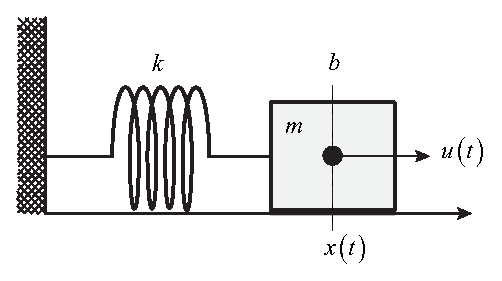
\includegraphics[width = 200pt, 
		keepaspectratio]{figures/state_fb/spring_mass/spring_mass.eps}
		\captionsetup{width=0.5\textwidth, font=small}
		\caption{Spring mass system with force input $u(t)$.}
		\label{spring_mass}
	\end{figure}
	Eq.~\eqref{spring_mass_eq_1} can be written in state space form as follows
	\begin{equation}\label{spring_mass_eq_2}
		\begin{aligned}
			\dot{x}(t) &= v(t) \\[6pt]
			\dot{v}(t) &= -\frac{k}{m}x(t) -\frac{b}{m}v(t) + \frac{1}{m}u(t)
		\end{aligned}
	\end{equation}
	or
	\begin{equation}\label{spring_mass_eq_3}
		\dot{\vec{x}}(t) = \tilde{\mathbf{A}}\vec{x}+\tilde{\mathbf{B}}x(t)
	\end{equation}
	where
	\begin{equation}\label{spring_mass_eq_4}
		\tilde{\mathbf{A}} = \begin{bmatrix}
			0&1 \\[6pt] -\frac{k}{m} &  -\frac{b}{m}
		\end{bmatrix}, \qquad
		\tilde{\mathbf{B}} = \begin{bmatrix}
			0 \\[6pt] \frac{1}{m}
		\end{bmatrix}
	\end{equation}
	supposing $k=\SI{1}{\newton\per\meter}$, $b=\SI{0}{\newton\second\per\meter}$ and $m=\SI{1}{\kilogram}$ we obtain
	\begin{equation}\label{spring_mass_eq_5}
		\tilde{\mathbf{A}} = \begin{bmatrix}
			0&1 \\[6pt] -1 &  0
		\end{bmatrix}, \qquad
		\tilde{\mathbf{B}} = \begin{bmatrix}
			0 \\[6pt] 1
		\end{bmatrix}
	\end{equation}
	where the natural evolution of the system can be represented by the phase 
	portrait of Figure~\ref{armonic_oscillator_2}\footnote{The phase portrait is built plotting the evolution $\vec{x}(t)$ in the plane $(x_1\ x_2)$. The evolution $\vec{x}(t)$ is computed by solving the system
		\begin{equation}
			\vec{x}(t) = e^{\tilde{\mathbf{A}}t}\vec{x}(0)
		\end{equation}
		where $\vec{x}(0)=\begin{bmatrix}
			1&0
		\end{bmatrix}^T$ is the initial condition. The solution can be computed as follows
		\begin{equation}
			\begin{aligned}
				\vec{x}(t) &= 
				\mathcal{L}^{-1}\Big\{\Big[s\mathbf{I}-\tilde{\mathbf{A}}\Big]^{-1}\Big\}\vec{x}(0)
				= \mathcal{L}^{-1}\Bigg\{\frac{1}{s^2+1}\begin{bmatrix} s & 1 \\[6pt] -1 & s 
				\end{bmatrix}\Bigg\}\vec{x}(0) = \\[6pt]
				&= \begin{bmatrix} \cos(t) & \sin(t) \\[6pt] -\sin(t) & \cos(t) \end{bmatrix}\vec{x}(0) = \begin{bmatrix} \cos(t) \\[6pt] -\sin(t) \end{bmatrix}
			\end{aligned}
		\end{equation}
		The phase portrait is build as parametric curve:
		\begin{equation}
			\mathcal{C}=\left\lbrace \begin{aligned}
				x_1(t)&=\cos(t) \\[6pt]
				x_2(t)&=-\sin(t) 
			\end{aligned}\right. 
		\end{equation}
	}. 
	
	Applying the state feedback to the system of Eq,~\eqref{spring_mass_eq_5} where matrix $\mathbf{K}$ is 
	computed by pole placement suppose the equivalent system has two poles as 
	$p_1=-1$ and $p_2=-1$ as follows
	\begin{equation}
		\text{find }\mathbf{K} \text{ such that 
		}\Big|s\mathbf{I}-\big(\tilde{\mathbf{A}}-\tilde{\mathbf{B}}\mathbf{K}\big)\Big|=(s+1)^2
	\end{equation}
	we obtain a system which its natural evolution can be 
	represented by the phase portrait of Figure~\ref{armonic_oscillator2_2}\footnote{Let's consider the case $\tilde{\mathbf{A}}-\mathbf{K}\tilde{\mathbf{B}}$ where
		\begin{equation}
			\vec{x}(t) = e^{\big(\tilde{\mathbf{A}}-\mathbf{K}\tilde{\mathbf{B}}\big)t}\vec{x}(0)
		\end{equation}
		where $\vec{x}(0)=\begin{bmatrix}
			1&0
		\end{bmatrix}^T$ is the initial condition and where $\tilde{\mathbf{A}}-\tilde{\mathbf{B}}\mathbf{K} = \begin{bmatrix}
			0 & 1 \\ -1 & -2
		\end{bmatrix}$. The solution can be computed as follows
		\begin{equation}
			\begin{aligned}
				\vec{x}(t) &= 
				\mathcal{L}^{-1}\Big\{\Big[s\mathbf{I}-\big(\tilde{\mathbf{A}}-\tilde{\mathbf{B}}\mathbf{K}\big)\Big]^{-1}\Big\}\vec{x}(0)
				= \mathcal{L}^{-1}\Bigg\{\frac{1}{(s+1)^2}\begin{bmatrix} s+2 & 1 \\[6pt] -1 & s 
				\end{bmatrix}\Bigg\}\vec{x}(0) = \\[6pt]
				&= \begin{bmatrix} \exp(-t)(t+1) & \exp(-t)t \\[6pt] -\exp(-t)t & -\exp(-t)(t-1) \end{bmatrix}\vec{x}(0) = \begin{bmatrix} \exp(-t)(t+1) \\[6pt] -\exp(-t)t \end{bmatrix}
			\end{aligned}
		\end{equation}
		The phase portrait is build as parametric curve:
		\begin{equation}
			\mathcal{C}=\left\lbrace \begin{aligned}
				x_1(t)&=\exp(-t)(t+1) \\[6pt]
				x_2(t)&=-\exp(-t)t 
			\end{aligned}\right. 
		\end{equation}
	}.
	\begin{figure}[H]
		\centering
		\begin{subfigure}{.5\textwidth}
			\centering
			\includegraphics[width = 200pt, 
			keepaspectratio]{figures/state_fb/spring_mass/armonic_oscillator_2.eps}
			\captionsetup{width=0.75\textwidth}		
			\caption{Phase portrait of the harmonic oscillator, where $\vec{x}(0) = 
				\begin{bmatrix} 1&0\end{bmatrix}$ and $u(t)=0$.}
			\label{armonic_oscillator_2}
		\end{subfigure}%
		\begin{subfigure}{.5\textwidth}
			\centering
			\includegraphics[width = 200pt, 
			keepaspectratio]{figures/state_fb/spring_mass/armonic_oscillator2_2.eps}
			\captionsetup{width=0.75\textwidth}		
			\caption{Phase portrait of the harmonic oscillator, where $\vec{x}(0) = 
				\begin{bmatrix} 1&0\end{bmatrix}$ and $u(t)=-\mathbf{K}\vec{x}(t)$.}
			\label{armonic_oscillator2_2}
		\end{subfigure}
		\caption{Phase portraits of the harmonic oscillator with and without state 
			feedback compensation.}
		\label{}
	\end{figure}
	$\triangleleft$ 
\end{example}


 
\section{Observability}
In this section we discuss the observability of linear systems. Consider the 
unforced system described by the following equations:
\begin{equation}\label{state_observer_eq_1}
	\dot{\vec x} = \tilde{\mathbf{A}} \vec x 
\end{equation}
\begin{equation}\label{state_observer_eq_2}
	\vec y = \mathbf{C} \vec x 
\end{equation}
where	\begin{itemize} 
	\item $\vec x = $ state vector (\textit{n-}vector)
	\item $\vec y = $ output vector (\textit{m-}vector). For SISO is $m=1$
	\item $ \tilde{\mathbf{A}} = $ \textit{n $\times$ n} matrix
	\item $ \mathbf{C} = $ \textit{m $\times$ n} matrix
\end{itemize}
The system is said to be completely observable if every initial state $\vec 
x(0)$ can be determined from the observation of $\vec y(t)$ over a finite time 
interval, $0 \leq t \leq t_1$. The system is, therefore, completely observable 
if every transition of the state eventually affects every element of the output 
vector. \textit{The concept of observability is useful in solving the problem 
of recostructioning of unmeasurable state variables from measurable variables 
in the minimum possible length of time.} 

The concept of observability is very important because, in practice, the 
difficulty encountered with state feedback control is that some of the state 
variables are not accessible for direct measurement, with the results that it 
become necessary to estimate the unmeasured state variables in order to 
construct the control signals. Such estimates of state variables are possible 
if only if the system is completely observable.

Consider the system
\begin{equation}
	\dot{\vec x} = \tilde{\mathbf{A}} \vec{x} + \tilde{\mathbf{B}} u
\end{equation}
\begin{equation}
y = \mathbf{C} \vec{x}
\end{equation}
where the state vector evolution is given as follows
\begin{equation}
	\vec x(t) = e^{\tilde{\mathbf{A}}t} \vec{x}(0) + \int\limits_0^t 
	e^{\tilde{\mathbf{A}}(t-\tau)}\tilde{\mathbf{B}} u(\tau)d\tau
\end{equation}
and where the output evolution as well
\begin{equation}
	y(t) = \mathbf{C}e^{\tilde{\mathbf{A}}t} \vec x(0) + 
	\mathbf{C}\int\limits_0^t 
	e^{\tilde{\mathbf{A}}(t-\tau)}\tilde{\mathbf{B}} u(\tau)d\tau
\end{equation}

Since the matrices $\tilde{\mathbf{A}}$, $\tilde{\mathbf{B}}$, $\mathbf{C}$ are 
known and 
$u(t)$ is also known, the last two terms on the right hand side of this last 
equation are known quantities. Therefore, they may be subtracted from the 
observed value of $y(t)$. Hence, for investigating a necessary and sufficient 
condition for complete observability, it suffices to consider the system 
described by Eq.~\eqref{state_observer_eq_1} and~\eqref{state_observer_eq_2}.

\vspace{5mm}
\textbf{Complete Observability of Continuos-Time Systems.} Consider the system 
described by Eq.~\eqref{state_observer_eq_1} and~\eqref{state_observer_eq_2}. 
The output quantity $y(t)$ is
\begin{equation}
y(t) = \mathbf{C}e^{\tilde{\mathbf{A}}t}\vec x(0)	
\end{equation}
where
\begin{equation}
	e^{\tilde{\mathbf{A}}t} = \sum_{k=0}^{n-1} \alpha_k(t)\tilde{\mathbf{A}}^k	
\end{equation}
where $n$ is the degree of the characteristic polynomial. 
Hence, we obtain
\begin{equation}
	y(t) = \sum_{k=0}^{n-1} \alpha_k(t)\mathbf{C}\tilde{\mathbf{A}}^k\vec x(0)
\end{equation}
or
\begin{equation} \label{state_observer_eq_3}
	y(t) = \alpha_0(t)\mathbf{C}\vec x(0) + 
	\alpha_1(t)\mathbf{C}\tilde{\mathbf{A}}\vec x(0) + ... + 
	\alpha_{n-1}(t)\mathbf{C}\tilde{\mathbf{A}}^{n-1}\vec x(0) \\
\end{equation}
If the system is completely observable, then, given the output $y(t)$ over a 
time interval $0 \leq t \leq t_1$, $\vec x(0)$ is uniquely determined from 
Eq.~\eqref{state_observer_eq_3}. It can be shown that this requires the rank of 
the $nm \times n$ matrix ($n \times n$ for SISO) to be $n$.
\begin{equation} \label{state_observer_eq_4}
\mathcal{O} = \begin{bmatrix}
	\mathbf{C}  \\
	\mathbf{C}\tilde{\mathbf{A}} \\
	\vdots \\
	\mathbf{C}\tilde{\mathbf{A}}^{n-1}
\end{bmatrix}
\end{equation}

From this analysis, we can state the condition for complete observability as 
follow: The system described by Eq.~\eqref{state_observer_eq_1} 
and~\eqref{state_observer_eq_2} is completely observable if and only if the $n 
\times nm$ matrix
\begin{equation}
\begin{bmatrix}
	\mathbf{C}  \\
	\mathbf{C}\tilde{\mathbf{A}} \\
	\vdots \\
	\mathbf{C}\tilde{\mathbf{A}}^{n-1}
\end{bmatrix}
\end{equation}
is of rank $n$ or has $n$ linearly independent column vectors. This matrix is 
called the \textit{observability matrix}.

\vspace{5mm}
\textbf{Condition for Complete Observability in the s Plane.} The conditions 
for complete observability can also be stated in terms of transfer functions. 
The necessary and sufficient conditions for complete observability is that no 
cancellation occur in the transfer function. \textit{If cancellation occurs, 
the cancelled mode cannot be observed in the output.}

\section{Principle of Duality}
We shall now discuss the relationship between controllability and 
observability. We shall introduce the principle of duality, due to Kalman, to 
clarify apparent analogies between controllability and observability.
Consider the system $S_1$ described by
\begin{equation} 
	\begin{split}
		\dot{\vec x} & = \mathbf{A}\vec x + \mathbf{B}\vec u \\
		\vec y & = \mathbf{C}\vec x
	\end{split}
\end{equation}
where	\begin{itemize} 
	\item $\vec x = $ state vector (\textit{n-}vector)
	\item $\vec u = $ input vector (\textit{r-}vector). For SISO is $r=1$
	\item $\vec y = $ output vector (\textit{m-}vector). For SISO is $m=1$
	\item $ \mathbf{A} = $ \textit{n $\times$ n} matrix
	\item $ \mathbf{B} = $ \textit{n $\times$ r} matrix
	\item $ \mathbf{C} = $ \textit{m $\times$ n} matrix
\end{itemize}
and the dual system $S_2$ described by
\begin{equation} 
	\begin{split}
		\dot{\vec z} & = \textbf{A}^*\vec z + \textbf{C}^*\vec v \\
		\vec n & = \mathbf{B}^*\vec z
	\end{split}
\end{equation}
where	\begin{itemize} 
	\item $\vec z = $ state vector (\textit{n-}vector)
	\item $\vec v = $ input vector (\textit{r-}vector). For SISO is $r=1$
	\item $\vec n = $ output vector (\textit{m-}vector). For SISO is $m=1$
	\item $ \mathbf{A}^* = $ conjugate transpose of $\mathbf{A} 
	\in\mathbb{C}^{n \times n}$ (transpose of $\mathbf{A}$ if 
	$\mathbf{A}\in\mathbb{R}^{n \times n}$) 
	\item $ \mathbf{B}^* = $ conjugate transpose of $\mathbf{B}\in\mathbb{C}^{n 
	\times r}$ (transpose of $\mathbf{B}$ if $\mathbf{B}\in\mathbb{R}^{n \times 
	r}$)
	\item $ \mathbf{C}^* = $ conjugate transpose of $\mathbf{C}\in\mathbb{C}^{m 
	\times n}$ (transpose of $\mathbf{C}$ if $\mathbf{C} \in  \rm \mathbb{R}^{m 
	\times n}$)
\end{itemize}
The principle of duality states that the system $S_1$ is completely state controllable (observable) if and only if system $S_2$ is completely observable (state controllable).
To verify this principle, let us write down the necessary and sufficient 
condition for complete state controllability and complete observability for 
system $S_1$ and $S_2$. 

\noindent For system $S_1$
\begin{enumerate}[label=\textbf{\arabic*}]
	\item A necessary and sufficient condition for complete state 
	controllability is that the rank of the $n 	\times nr$ matrix 
	$$
	\begin{bmatrix}
		\mathbf{B} & \mathbf{AB} & \dots & \mathbf{A}^{n-1}\mathbf{B}
	\end{bmatrix}
	$$
	be $n$.
	\item A necessary and sufficient condition for complete state observability is that the rank of the $n 	\times nm$ matrix 
	$$
	\begin{bmatrix}
		\mathbf{C}^* & \mathbf{A}^*\mathbf{C}^* & \dots & (\mathbf{A}^*)^{n-1}\mathbf{C}^*
	\end{bmatrix} = 
	\begin{bmatrix}
		\mathbf{C}  \\
		\mathbf{CA} \\
		\vdots \\
		\mathbf{CA}^{n-1}
	\end{bmatrix}^*
	$$
	be $n$.
\end{enumerate}

\noindent For system $S_2$
\begin{enumerate}[label=\textbf{\arabic*}]
	\item A necessary and sufficient condition for complete state 
	controllability is that the rank of the $n 	\times nm$ matrix 
	$$
	\begin{bmatrix}
		\mathbf{C}^* & \mathbf{A}^*\mathbf{C}^* & \dots & (\mathbf{A}^*)^{n-1}\mathbf{C}^*
	\end{bmatrix}= 
	\begin{bmatrix}
		\mathbf{C}  \\
		\mathbf{CA} \\
		\vdots \\
		\mathbf{CA}^{n-1}
	\end{bmatrix}^*
	$$
	be $n$.
	\item A necessary and sufficient condition for complete state observability 
	is that the rank of the $n 	\times nr$ matrix 
	$$
	\begin{bmatrix}
		\mathbf{B} & \mathbf{AB} & \dots & \mathbf{A}^{n-1}\mathbf{B}
	\end{bmatrix}
	$$
	be $n$.
\end{enumerate}
{By use of this principle, the observability of a given system can be checked 
by testing the state controllability of its dual.}

\section{State Observer} 
In the pole placement approach to the design of control systems, we assume that 
all state variable are available for feedback. In practice, however, not all 
state variables are available for feedback. Then we need to estimate 
unavailable state variables.

\vspace{5mm}
\textbf{State Observer}. A state observer estimates the state variables based 
on the measurements of the output and control variables. \textit{State 
observers can be designed if and only if the observability condition is 
satisfied.}
Considering the plant defined by
\begin{equation} \label{state_observer_1}
	\begin{split}
		\dot{\vec x} & = \tilde{\mathbf{A}}\vec{x} + \tilde{\mathbf{B}}u \\[6pt]
		y & = \mathbf{C}\vec{x}
	\end{split}
\end{equation}
The observer is a subsystem to reconstruct the state vector of the plant. The 
mathematical model of the observer is basically the same as that of the plant, 
except that we include an additional term that includes the estimation error to 
compensate for inaccuracies in matrices $\tilde{\mathbf{A}}$ and 
$\tilde{\mathbf{B}}$ and the lack of the initial error.The estimation error or 
the observation error is the difference between the measured output and the 
estimated output. The initial error is the difference between the initial state 
and the initial estimated state. Thus, we define the mathematical model of the 
observer to be
\begin{equation} \label{state_observer_2}
	\begin{split}
		\dot{\hat{\vec{x}}} & = \tilde{\mathbf{A}}\hat{\vec x} + 
		\tilde{\mathbf{B}}\vec u + \mathbf{L}(y - \mathbf{C}\hat{\vec x}) 
		\\
		& = (\tilde{\mathbf{A}}-\mathbf{L}\mathbf{C})\hat{\vec x} + 
		\tilde{\mathbf{B}}u + \mathbf{L}y
	\end{split}
\end{equation}
where $\hat{\vec x}$ is the estimated state and $\mathbf{C}\hat{\vec x}$ is the 
estimated output. \textit{The inputs of the observer are the output $\vec y$ 
and the control input $\vec u$}. Matrix $\mathbf{L}$ which is called the 
observer gain matrix, is a weighting matrix to the correction term involving 
the difference between the measured output $\vec y$ and the estimated output 
$\mathbf{C}\hat{\vec x}$. this term continuously corrects the model output and 
improves 
the performance of the observer. Figure~\ref{figure_state_observer} shows the 
block diagram of the system and the full-order state observer.
The order of the state observer that will be discussed here is the same as that 
of the plant.

To obtain the observer error equation, let us subtract 
Eq.~\eqref{state_observer_2} from 
Eq.~\eqref{state_observer_1}:
\begin{equation} \label{state_observer_3}
	\begin{split}
		\dot{\vec{x}} - \dot{\hat{\vec x}} & = \tilde{\mathbf{A}}\vec x - 
		\tilde{\mathbf{A}}\hat{\vec x} - \mathbf{L}(\mathbf{C}\vec x - 
		\mathbf{C}\hat{\vec{x}}) \\
		& = (\mathbf{\mathbf{A}}-\mathbf{L}\mathbf{C})(\vec{x} - \hat{\vec{x}})
	\end{split}
\end{equation}
Define the difference between $\vec{x}$ and $\hat{\vec{x}}$ as the error vector 
$\vec{e}$, or
\begin{equation} \label{state_observer_4}
	\vec{e} = \vec{x} - \hat{\vec{x}}
\end{equation}
the equation (\ref{state_observer_3}) becomes
\begin{equation} \label{state_observer_5}
	\dot{\vec{e}} = (\tilde{\mathbf{A}}-\mathbf{LC})\vec{e}
\end{equation}
From Eq.~\eqref{state_observer_5}, we see that the dynamic behaviour of the 
error vector is 
determined by the eigenvalues of matrix $(\tilde{\mathbf{A}}-\mathbf{LC})$. If 
matrix $(\tilde{\mathbf{A}}-\mathbf{LC})$ is a stable matrix, the error vector 
will converge to zero for any initial error vector $\vec e(0)$. That is, 
$\hat{\vec x}(t)$ will 
converge to $\vec x(t)$ regardless of the value of $\vec x(0)$ and 
$\hat{\vec{x}}(0)$. If the eigenvalues of the matrix 
$(\tilde{\mathbf{A}}-\mathbf{LC})$ are chosen in such a way that the dynamic 
behaviour of the error vector is asymptotically stable and is adequately fast, 
then any error vector will tend to zero (the origin) with an adequate speed.
If the plant is completely observable, then it can be proved that it is 
possible to choose matrix $\mathbf{L}$ such that 
$(\tilde{\mathbf{A}}-\mathbf{LC})$ has 
arbitrarily desired eigenvalues. That is, the observer gain matrix $\mathbf{L}$ 
can be determined to yield the desired matrix 
$(\tilde{\mathbf{A}}-\mathbf{LC})$. 
\begin{figure}[H]
	\centering
	\begin{subfigure}{.75\textwidth}
	\centering
	\includegraphics[width = 340pt, 
	keepaspectratio]{figures/state_observer_1.eps}
	\captionsetup{width = 0.5\textwidth}
	\caption{Physical Plant in the form of state space representation.}
	\label{figure_state_observer1}
	\end{subfigure} 

	\begin{subfigure}{.75\textwidth}
	\centering
	\includegraphics[width = 340pt, 
	keepaspectratio]{figures/state_observer_2.eps}
		\captionsetup{width = 0.5\textwidth}
		\caption{Physical Plant in the form of transfer function.}
	\label{figure_state_observer2}
	\end{subfigure}
	\caption{Full-order state observer.}
	\label{figure_state_observer}
\end{figure}

\vspace{5mm}
\textbf{Dual Problem}. The design of the full-order observer becomes that of determining an appropriate $\mathbf{L}$ such that $(\mathbf{A-LC})$ has desired eigenvalues. Thus the problem here become the same as the pole placement problem and this property is called duality.

Consider the system defined by
\begin{equation}\label{duality_eq_1}
	\begin{split}
		\dot{\vec x} & = \mathbf{A}\vec x + \mathbf{B}u \\
		y & = \mathbf{C}\vec x
	\end{split}
\end{equation}
In designing the full-order state observer, we may solve the dual problem, that is, solve the pole-placement problem for the dual system
\begin{equation}\label{duality_eq_2}
	\begin{split}
		\dot{\vec z} & = \mathbf{A}^*\vec z + \mathbf{B}^*v \\
		n & = \mathbf{C}^*\vec z
	\end{split}
\end{equation}
assuming the control signal $v$ to be
\begin{equation}\label{duality_eq_3}
v=-\mathbf{K}\vec z
\end{equation}
If the dual system is completely state controllable, then the state feedback gain matrix $\mathbf{K}$ can be determined such that matrix $(\mathbf{A}^*-\mathbf{C}^*\mathbf{K})$ will yield a set of the desired eigenvalues.
If $\mu_1$,$\mu_2$,$...$,$\mu_n$ are the desired eigenvalues of the state observer matrix, then by taking the same $\mu_i$'s as the desired eigenvalues of the state-feedback gain matrix of the dual system, we obtain
\begin{equation}\label{duality_eq_4}
|s\mathbf{I-(A^* - C^*K)}|= (s-\mu_1)(s-\mu_2)...(s-\mu_n)
\end{equation}
Noting that the eigenvalues of $\mathbf{A}^*-\mathbf{C}^*\mathbf{K}$ and those of $\mathbf{A-K}^*\mathbf{C}$ are the same, we have 
\begin{equation}\label{duality_eq_5}
|s\mathbf{I}-(\mathbf{A}^* - \mathbf{C}^*\mathbf{K})|= |s\mathbf{I}-(\mathbf{A} - \mathbf{K^*C})|
\end{equation}
Comparing the characteristic polynomial $|s\mathbf{I-(A - K^*C)}|$ and the characteristic polynomial $|s\mathbf{I-(A - LK)}|$ for the observer system we find that $\mathbf{L}$ and $\mathbf{K}^*$ are related by
\begin{equation}\label{duality_eq_6}
\mathbf{L=K^*}
\end{equation}
Thus, using the matrix $\mathbf{K}$ determined by pole placement approach in 
the dual system, the observer gain matrix $\mathbf{L}$ for the original system 
can be determined by using the relationship $\mathbf{L=K^*}$.

\vspace{5mm}
\textbf{Necessary and Sufficient Condition for State Observation}. As discussed, a necessary and sufficient condition for the determination of the observer gain matrix $\mathbf{L}$ for the desired eigenvalues of $\mathbf{A-LC}$ is that the dual of the original system
\begin{equation}\label{duality_eq_7}
	\dot{\vec z} = \mathbf{A}^*\vec z + \mathbf{C}^*v
\end{equation}
be completely state controllable. The complete state controllability condition for this dual system is that the rank of 
\begin{equation}\label{duality_eq_8}
	\begin{bmatrix}
		\mathbf{C}^* & \mathbf{A^*C^*} & \dots & (\mathbf{A}^*)^{n-1}\mathbf{C}^*
	\end{bmatrix}= 
	\begin{bmatrix}
		\mathbf{C}  \\
		\mathbf{CA} \\
		\vdots \\
		\mathbf{CA}^{n-1}
	\end{bmatrix}^*
\end{equation}
be $n$. This is the condition for complete observability of the original system 
defined by Eq.~\eqref{duality_eq_1}.

\vspace{5mm}
\textbf{Direct-Substitution Approach to Obtain State Observer Gain Matrix $\mathbf{L}$}. Similar to the case of pole placement, if the system is of low order, then direct substitution of matrix $\mathbf{L}$ into the desired characteristic polynomial may be simpler. For example, if $\vec x$ is a 3-vector, then write the observer gain matrix $\mathbf{L}$ as
\begin{equation} 
\mathbf{L}=\begin{bmatrix}
	l_1\\
	l_2\\
	l_3
\end{bmatrix}
\end{equation}
Substitute this $\mathbf{L}$ matrix into the desired characteristic polynomial:
\begin{equation} 
|s\mathbf{I-(A - LC)}|= (s-\mu_1)(s-\mu_2)(s-\mu_3)
\end{equation}
By equating the coefficient of the like powers of ts on both sides of this last equation, we can determine the values of $l_1$,$l_2$ and $l_3$.

\vspace{5mm}
\textbf{Ackermann's Formula}.
\textbf{Let's go back to state feedback design} and we consider the system defined by
\begin{equation} \label{ackermann_1}
	\begin{split}
		\dot{\vec x} & = \mathbf{A}\vec x + \mathbf{B}u \\
		y & = \mathbf{C}\vec x
	\end{split}
\end{equation}
Use of the state feedback control 
\begin{equation*}
	u = -\mathbf{K}\vec x
\end{equation*}
modifies the system equation to 
\begin{equation} \label{ackermann_2}
	\dot{\vec x} = \mathbf{\Big[A-BK\Big]}\vec x
\end{equation}
Let us define
\begin{equation*}
	\tilde{\mathbf{A}} = \mathbf{\Big[A-BK\Big]}
\end{equation*}
The desired characteristic equation is

\begin{equation} \label{ackermann_3}
	\begin{split}
		|s\mathbf{I-(A - LC)}| & = |s\mathbf{I}-\tilde{\mathbf{A}}| = (s-\mu_1)(s-\mu_2)...(s-\mu_n) \\
		& = s^n +\alpha_1s^{n-1}+...+\alpha_{n-1}s+\alpha_n = 0
	\end{split}
\end{equation}
Since the \textbf{Cayley-Hamilton} theorem states that $\tilde{\mathbf{A}}$ satisfies its own characteristic equation, we have
\begin{equation} \label{ackermann_4}
	\phi(\tilde{\mathbf{A}}) = \tilde{\mathbf{A}}^n+\alpha_1\tilde{\mathbf{A}}^{n-1}+...+\alpha_{n-1}\tilde{\mathbf{A}}+\alpha_n\mathbf{I} = 0
\end{equation}
We shall utilize Eq.~\eqref{ackermann_4} to derive Ackermann's formula. We 
consider the case $n=3$.
\begin{equation*}
	\begin{split}
		\mathbf{I} & = \mathbf{I} \\
		\tilde{\mathbf{A}} & = \mathbf{A-BK} \\
		\tilde{\mathbf{A}}^2 & = \mathbf{(A-BK)^2=A^2-ABK-BK}\tilde{\mathbf{A}} \\
		\tilde{\mathbf{A}}^3 & = \mathbf{(A-BK)}^3=\mathbf{A^3BK-A^2BK-ABK}\tilde{\mathbf{A}}-\mathbf{BK}\tilde{\mathbf{A}}^2
	\end{split}
\end{equation*}

\begin{equation} \label{ackermann_5}
	\begin{split}
		\alpha_3\mathbf{I}+\alpha_2\tilde{\mathbf{A}}+\alpha_1\tilde{\mathbf{A}}^2+\tilde{\mathbf{A}}^3 = & \\
		= & \:\alpha_3\mathbf{I}+\alpha_2\mathbf{(A-BK)}+\alpha_1(\mathbf{A^2-ABK-BK}\tilde{\mathbf{A}})+\\
		& +\mathbf{A}^3-\mathbf{A}^2\mathbf{BK} -\mathbf{ABK}\tilde{\mathbf{A}}-\mathbf{BK}\tilde{\mathbf{A}}^2 = \\
		& \alpha_3\mathbf{I}+\alpha_2\mathbf{A}+\alpha_1\mathbf{A}^2+\mathbf{A}^3-\alpha_2\mathbf{BK}-\alpha_1\mathbf{ABK}+\\
		&-\alpha_1\mathbf{BK}\tilde(\mathbf{A})-\mathbf{A^2BK-ABK}\tilde(\mathbf{A})-\mathbf{BK}\tilde{\mathbf{A}}^2
	\end{split}
\end{equation}
Referring to Eq.~\eqref{}, we have
\begin{equation*}
	\alpha_3\mathbf{I}+\alpha_2\tilde{\mathbf{A}}+\alpha_1 
	\tilde{\mathbf{A}}^2+\tilde{\mathbf{A}}^3=\phi(\tilde{\mathbf{A}})=0
\end{equation*}
Also we have
\begin{equation*}
	\alpha_3\mathbf{I}+\alpha_2\mathbf{A}+\alpha_1\mathbf{A}^2+ 
	\mathbf{A}^3=\phi(\mathbf{A})\not =0
\end{equation*}
Substituting the last two equations into equation (\ref{eq:14}) we have
\begin{equation*}
	\phi(\tilde{\mathbf{A}})=\phi(\mathbf{A})-\alpha_2\mathbf{BK}- 
	\alpha_1\mathbf{BK}\tilde{\mathbf{A}}-BK\tilde{\mathbf{A}}^2- 
	\alpha_1\mathbf{ABK-ABK}\tilde{\mathbf{A}}-\mathbf{A^2BK}
\end{equation*}
Since $\phi(\tilde{\mathbf{A}})=0$ we obtain

\begin{equation} \label{ackermann_6}
	\begin{split}
		\phi(\tilde{\mathbf{A}}) = & \:\mathbf{B}(\alpha_2\mathbf{K}+\alpha_1\mathbf{K}\tilde{\mathbf{A}}+\mathbf{K}\tilde{\mathbf{A}}^2)+\mathbf{AB}(\alpha_1\mathbf{K}+\mathbf{K}\tilde{\mathbf{A}})+\mathbf{A}^2\mathbf{BK}+\\
		= & \: 	
		\begin{bmatrix}
			\mathbf{B} & \mathbf{AB} & \mathbf{A}^2\mathbf{B}
		\end{bmatrix}
		\begin{bmatrix}
			\alpha_2\mathbf{K}+\alpha_1\mathbf{K}\tilde{\mathbf{A}}+\mathbf{K}\tilde{\mathbf{A}}^2 \\ 
			\alpha_1\mathbf{K}+\mathbf{K}\tilde{\mathbf{A}} \\
			\mathbf{K}
		\end{bmatrix}
	\end{split}
\end{equation}
Since the system is completely state controllable, the inverse of the controllability matrix
\begin{equation}
	\begin{bmatrix}
		\mathbf{B} & \mathbf{AB} & \mathbf{A}^2\mathbf{B}
	\end{bmatrix}
\end{equation}
exists. Premultiplying both side of Eq.~\eqref{} by the inverse of the 
controllability matrix, we obtain
\begin{equation}
	\begin{bmatrix}
		\mathbf{B} & \mathbf{AB} & \mathbf{A}^2\mathbf{B}
	\end{bmatrix}^{-1} \phi(\mathbf{A})=
	\begin{bmatrix}
		\alpha_2\mathbf{K}+\alpha_1\mathbf{K}\tilde{\mathbf{A}}+k\tilde{\mathbf{A}}^2 \\ 
		\alpha_1\mathbf{K}+\mathbf{K}\tilde{\mathbf{A}} \\
		\mathbf{K}
	\end{bmatrix}
\end{equation}
Premultiplying both sides of this last equation by $\begin{bmatrix} 0&0&1\end{bmatrix}$, we obtain 
\begin{equation}
	\begin{bmatrix} 
		0&0&1
	\end{bmatrix}
	\begin{bmatrix}
		\mathbf{B} & \mathbf{AB} & \mathbf{A}^2\mathbf{B}
	\end{bmatrix}^{-1} \phi(\mathbf{A})=
	\begin{bmatrix} 
		0&0&1
	\end{bmatrix}
	\begin{bmatrix}
		\alpha_2\mathbf{K}+\alpha_1\mathbf{K}\tilde{\mathbf{A}}+k\tilde{\mathbf{A}}^2 \\ 
		\alpha_1\mathbf{K}+\mathbf{K}\tilde{\mathbf{A}} \\
		\mathbf{K}
	\end{bmatrix} = \mathbf{K}
\end{equation}
Which cab be rewritten as
\begin{equation*}
	\mathbf{K} = \begin{bmatrix} 
		0&0&1
	\end{bmatrix}
	\begin{bmatrix}
		\mathbf{B} & \mathbf{AB} & \mathbf{A}^2\mathbf{B}
	\end{bmatrix}^{-1} \phi(\mathbf{A})
\end{equation*}
This last equation gives the required state feedback gain matrix $\mathbf{K}$.

For an arbitrary positive integer $n$ we have
\begin{equation} \label{ackermann_7}
	K = \begin{bmatrix} 
		0&0&...&1
	\end{bmatrix}
	\begin{bmatrix}
		\mathbf{B} & \mathbf{AB} & ...& \mathbf{A}^{n-1}\mathbf{B}
	\end{bmatrix}^{-1} \phi(\mathbf{A})
\end{equation}
Which is known as Ackermann's formula for the determination of the state 
feedback gain matrix $\mathbf{K}$.

For the duality proprieties we can modify the above Ackermann's formula to
\begin{equation} \label{ackermann_8}
	\mathbf{K} = \begin{bmatrix} 
		0&0&...&1
	\end{bmatrix}
	\begin{bmatrix}
		\mathbf{C}^* & \mathbf{A}^*\mathbf{C}^* & ...& (\mathbf{A}^*)^{n-1}\mathbf{C}^*
	\end{bmatrix}^{-1} \phi(\mathbf{A}^*)
\end{equation}
Thus
\begin{equation} \label{ackermann_9}
	\mathbf{L} =\mathbf{K}^*= \phi(\mathbf{A}) \begin{bmatrix} 
		\mathbf{C} \\
		\mathbf{CA} \\
		\vdots \\
		\mathbf{CA}^{n-2} \\
		\mathbf{CA}^{n-1}
	\end{bmatrix}^{-1}
	\begin{bmatrix}
		0 \\
		0 \\
		\vdots \\
		0 \\
		1
	\end{bmatrix}
\end{equation}

\vspace{5mm}
\textbf{Effects of the Addition of the State Observer to the State Feedback.} 
In the pole-placement design process, we assumed that the actual state $\vec 
x(t)$ was available for feedback. In practice, however, the actual state $\vec 
x(t)$ may not be measurable, so we will need to design an observer and use the 
observed state $\hat{\vec x}(t)$ for feedback as shown in 
Figure~\ref{figure_state_observer_comp}
\begin{figure}
	\centering
	\includegraphics[width = 380pt, keepaspectratio]{figures/state_observer_compensator_1.eps}
		\captionsetup{width=0.5\textwidth, font=small}		
		\caption{Observed state feedback control system.}
	\label{figure_state_observer_comp}
\end{figure}
The design process, therefore, becomes a two stage process, the first stage being the determination of the feedback gain matrix $\mathbf{K}$ to yield the desired characteristic equation and the second stage being the determination of the observer gain matrix $\mathbf{L}$ to yield the desired observer characteristic equation.

Let us now investigate the effects of the use of the observed state $\hat{\vec x}(t)$, rather than the actual state $\vec x(t)$, on the characteristic equation of a closed-loop control system.

Consider the completely state controllable and completely observable system 
defined by the equations
\begin{equation*}
	\begin{split}
		\dot{\vec x}(t) & = \tilde{\mathbf{A}}\vec x(t) + 
		\tilde{\mathbf{B}}u(t) \\
		y(t) & = \mathbf{C}\vec x(t)
	\end{split}
\end{equation*} 
For the state feedback control based on the observed state $\hat{\vec x}(t)$ 
\begin{equation*}
	\begin{split}
		u(t)=-\mathbf{K}\hat{\vec x}(t)
	\end{split}
\end{equation*} 
The state equation becomes
\begin{equation} \label{ackermann_10}
	\begin{split}
		\dot{\vec x}(t)=\tilde{\mathbf{A}}\vec 
		x(t)-\tilde{\mathbf{B}}\mathbf{K}\hat{\vec x}(t) = 
		\Big[\tilde{\mathbf{A}}-\tilde{\mathbf{B}}\mathbf{K}\Big]\vec x(t) + 
		\tilde{\mathbf{B}}\mathbf{K}\Big[\vec x(t) - 
		\hat{\vec x}(t)\Big]
	\end{split}
\end{equation} 
The difference between the actual state $\vec x(t)$ and the observed state $\hat{\vec x}(t)$ has been defined as the error $\vec e(t)$:
\begin{equation*}
	\begin{split}
		\vec e(t)=\vec x(t) - \hat{\vec x}(t)
	\end{split}
\end{equation*} 
Substitution of the error vector $\vec e(t)$ into the Eq.~\eqref{ackermann_10} 
gives
\begin{equation} \label{ackermann_11}
	\begin{split}
		\dot{\vec x}(t) = 
		\Big[\tilde{\mathbf{A}}-\tilde{\mathbf{B}}\mathbf{K}\Big]\vec x(t) + 
		\tilde{\mathbf{B}}\mathbf{K}\vec{e}(t)
	\end{split}
\end{equation} 
While the observer error equation is given by
\begin{equation} \label{ackermann_12}
	\begin{split}
		\dot{\vec e}(t)= \Big[\tilde{\mathbf{A}}-\mathbf{LC}\Big]\vec e(t)
	\end{split}
\end{equation}
Combining Eq.~\eqref{ackermann_11} and~\eqref{ackermann_12} we obtain
\begin{equation} \label{ackermann_13}
	\begin{bmatrix} 
		\dot{\vec x}(t) \\[6pt]
		\dot{\vec e}(t) 
	\end{bmatrix} =
	\begin{bmatrix}
		\tilde{\mathbf{A}}-\tilde{\mathbf{B}}\mathbf{K} & 
		\tilde{\mathbf{B}}\mathbf{K} \\[6pt]
		0 & \tilde{\mathbf{A}}-\mathbf{LC} 
	\end{bmatrix}
	\begin{bmatrix} 
		\vec x(t) \\[6pt]
		\vec e(t)
	\end{bmatrix}
\end{equation}
Eq.~\eqref{ackermann_13} describes the dynamics of the observed state feedback 
control system.
The characteristic equation for the system is
\begin{equation} 
	\begin{vmatrix}
		s\mathbf{I} -\tilde{\mathbf{A}}+\tilde{\mathbf{B}}\mathbf{K} & 
		-\tilde{\mathbf{B}}\mathbf{K} \\[6pt]
		0 & s\mathbf{I} - \tilde{\mathbf{A}}+\mathbf{LC} 
	\end{vmatrix} = 0
\end{equation}
or 
\begin{equation} 
	\Big|s\mathbf{I} -\tilde{\mathbf{A}}+\tilde{\mathbf{B}}\mathbf{K}\Big|\Big| 
	s\mathbf{I} - \tilde{\mathbf{A}}+\mathbf{LC}\Big| = 0
\end{equation}
Notice that the closed-loop poles of the observed-state feedback control system consist of the poles due to the pole placement design alone and the poles due to the observer design alone. This means that the pole-placement design and the and the observer design are independent of each other.
They can be designed separately and combined to form the observed state 
feedback control system. Note that, if the order of the plant is $n$, then the 
observer is also of $n$th order and the resulting characteristic equation for 
the entire closed loop system become or order $2n$.

Suppose now to use the following input quantity:
\begin{equation}
	\begin{split}
		u(t)=-\mathbf{K}\hat{\vec x}(t) + Nr(t)
	\end{split}
\end{equation} 
The equation of the state observer become the following:
\begin{equation}
	\begin{split}
		\dot{\hat{\vec x}}(t) = 
		\Big[\tilde{\mathbf{A}}-\tilde{\mathbf{B}}\mathbf{K}-\mathbf{LC}\Big] 
		\hat{\vec{x}}(t)+\tilde{\mathbf{B}}\mathbf{N}+\mathbf{L}y(t)
	\end{split}
\end{equation} 
as shown in Figure~\ref{figure_state_observer_comp}.

\vspace{5mm}
\textbf{Transfer Function of the Observer-Based Controller}. Considering the 
plant defined by
\begin{equation}
	\begin{split}
		\dot{\vec x}(t) & = \tilde{\mathbf{A}}\vec{x}(t)+ 
		\tilde{\mathbf{B}}u(t) \\
		y(t) & = \mathbf{C}\vec x(t)
	\end{split}
\end{equation} 
Assume that the plant is completely observable. Assume that we use 
observed-state feedback control $u=-\mathbf{K}\hat{\vec{x}}$. Than the equation 
for the observer are given by
\begin{equation} \label{ackermann_14}
	\dot{\hat{\vec x}}(t) = \Big[\mathbf{A} - \mathbf{LC} - 
	\tilde{\mathbf{B}}\mathbf{K}\Big]\hat{\vec x}(t) + 
	\mathbf{L}y(t) \\
\end{equation}
where
\begin{equation} \label{ackermann_15}
	u(t) = -\mathbf{K}\hat{\vec x}(t)
\end{equation}
By taking the Laplace transform of Eq.~\eqref{ackermann_15} we obtain 
\begin{equation}
	\hat{\vec{X}}(s) = \Big[s\mathbf{I} - \tilde{\mathbf{A}} + \mathbf{LC} + 
	\tilde{\mathbf{B}}\mathbf{K}\Big]^{-1}\mathbf{L}Y(s)
\end{equation} 
By substituting $\hat{X}(s)$ into the Laplace transform of 
Eq.~\eqref{ackermann_15}, we obtain
\begin{equation}\label{ackermann_16}
	U(s) = -\mathbf{K}\Big[s\mathbf{I} - \tilde{\mathbf{A}} + \mathbf{LC} + 
	\tilde{\mathbf{B}}\mathbf{K}\Big]^{-1}\mathbf{L}Y(s)
\end{equation} 
Then the transfer function $U(s)/Y(s)$ can be obtained as 
\begin{equation}
	\frac{U(s)}{Y(s)} = -\mathbf{K}\Big[s\mathbf{I} - \tilde{\mathbf{A}} + 
	\mathbf{LC} + \tilde{\mathbf{B}}\mathbf{K}\Big]^{-1}\mathbf{L}
\end{equation} 
Hence we call the transfer function 
\begin{equation}\label{ackermann_17}
	\frac{U(s)}{-Y(s)} = \mathbf{K}\Big[s\mathbf{I} - \tilde{\mathbf{A}} + 
	\mathbf{LC} + \tilde{\mathbf{B}}\mathbf{K}\Big]^{-1}\mathbf{L}
\end{equation} 
the observer-based controller transfer function or, simply, the 
observer-controller transfer function. 

\vspace{5mm}
Note that the observer-controller matrix
\begin{equation}
	\tilde{\mathbf{A}} - \mathbf{LC} - \tilde{\mathbf{B}}\mathbf{K} 
\end{equation} 
may or may not be stable, although 
$\tilde{\mathbf{A}}-\tilde{\mathbf{B}}\mathbf{K}$ and $\tilde{\mathbf{A}} - 
\mathbf{LC}$ are 
chosen to be stable. In fact, in some cases the matrix 
$\tilde{\mathbf{A}}-\mathbf{LC}-\tilde{\mathbf{B}}\mathbf{K}$ may 
be poorly stable or even unstable.

\vspace{5mm}
\begin{example}[\textbf{Double Integrator Observer}]\label{DoubleIntegratorObserver}
Consider the plant
\begin{equation}\label{DoubleIntegratorObserver_eq1}
	\left\lbrace \begin{aligned}
		&\ddot{x}=0 \\
		&y=x_1
	\end{aligned}\right. 
\end{equation}
and by its state space representation as follows
\begin{equation}\label{DoubleIntegratorObserver_eq2}
	\left\lbrace \begin{aligned}
		\dot{\vec{x}}(t)=\tilde{\mathbf{A}}\vec{x}(t) \\[6pt]
		y(t)=\mathbf{C}\vec{x}(t)
	\end{aligned}\right. 
\end{equation}
where $\tilde{\mathbf{A}}=\begin{bmatrix} 0&1\\0&0 \end{bmatrix}$ and 
$\mathbf{C}=\begin{bmatrix} 1&0 \end{bmatrix}$.

The equations which describe the \textbf{double integrator observer} can be 
written as follows
\begin{equation}\label{DoubleIntegratorObserver_eq3}
	\begin{aligned}
		\dot{\hat{\vec{x}}}(t)=\tilde{\mathbf{A}}\hat{\vec{x}}(t)+\tilde{\mathbf{L}}\Big(y(t)-\mathbf{C}\hat{\vec{x}}(t)\Big)
	\end{aligned}
\end{equation}

Eq.~\eqref{DoubleIntegratorObserver_eq3} can also be written as follows
\begin{equation}\label{DoubleIntegratorObserver_eq4}
	\left\lbrace \begin{aligned}
		\dot{\hat{x}}_1(t) &= \hat{x}_2(t) + \tilde{l}_1\Big[x_1(t) - 
		\hat{x}_1(t)\Big] 
		\\[6pt]
		\dot{\hat{x}}_2(t) &= \tilde{l}_2\Big[x_1(t) - \hat{x}_1(t) \Big]
	\end{aligned}\right. 
\end{equation}
where $y(t) = x_1(t)$ and $\tilde{\mathbf{L}}=\begin{bmatrix} 
\tilde{l}_1&\tilde{l}_2 \end{bmatrix}^T$;

The calculation of the observer gain matrix $\tilde{\mathbf{L}}$ can be done 
using the 
pole placement procedure e.g. applying the \texttt{acker} command in matlab
\begin{equation}\label{DoubleIntegratorObserver_eq5}
	\texttt{Ltilde = (acker(Atilde',C',[-p1, -p2]))';}
\end{equation}

The graphical representation of Eq.~\eqref{DoubleIntegratorObserver_eq4} 
results as shown in Figure~\ref{DoubleIntegratorObserver_ct_splitted}
\begin{figure}[H]
	\centering
	\includegraphics[width = 320pt,	keepaspectratio] 
	{figures/double_integrator_observer.eps}
	\captionsetup{width=0.5\textwidth, font=small}		
	\caption{Double Integrator Observer.}
	\label{DoubleIntegratorObserver_ct_splitted}
\end{figure}

The discrete time representation of the dynamical system $\ddot{x}=0$, can be 
represented as follows
\begin{equation}\label{DoubleIntegratorObserver_eq6}
	\left\lbrace \begin{aligned}
		{\vec{x}}(k+1)=\mathbf{A}\vec{x}(k) \\
		y(k)=\mathbf{C}\vec{x}(k)
	\end{aligned}\right. 
\end{equation}
where $\mathbf{A}=\mathbf{I}+\tilde{\mathbf{A}}t_s=\begin{bmatrix} 1&t_s\\0&1 
\end{bmatrix}$ and 
$\mathbf{C}=\begin{bmatrix} 1&0 \end{bmatrix}$.

The equation of the state observer in the discrete time domain results as 
follows
\begin{equation}\label{DoubleIntegratorObserver_eq7}
	\begin{aligned}
		{\hat{\vec{x}}}(k+1)={\mathbf{A}}\hat{\vec{x}}(k)+\mathbf{L}\Big(y(k)-\mathbf{C}\hat{\vec{x}}(k)\Big)
	\end{aligned}
\end{equation}
which can be represented as well
\begin{equation}\label{DoubleIntegratorObserver_eq8}
	\left\lbrace \begin{aligned}
		{\hat{x}}_1(k+1) & = \hat{x}_1(k) + \hat{x}_2(k)t_s + l_1\Big[x_1(k) 
		- \hat{x}_1(k)\Big] \\[6pt]
		{\hat{x}}_2(k+1) & = \hat{x}_2(k) + l_2\Big[x_1(k) - \hat{x}_1(k) 
		\Big]
	\end{aligned}\right. 
\end{equation}
where $y(k) = x_1(k)$ and $\mathbf{L}=\begin{bmatrix} l_1&l_2 
\end{bmatrix}^T$
The calculation of the $\mathbf{L}$ gain can be done using the \texttt{acker} 
command in matlab: 
$$\texttt{L = (acker(A',C',[exp(-p1*ts), exp(-p2*ts)]))';}$$
with the following graphical representation
\begin{figure}[H]
	\centering
	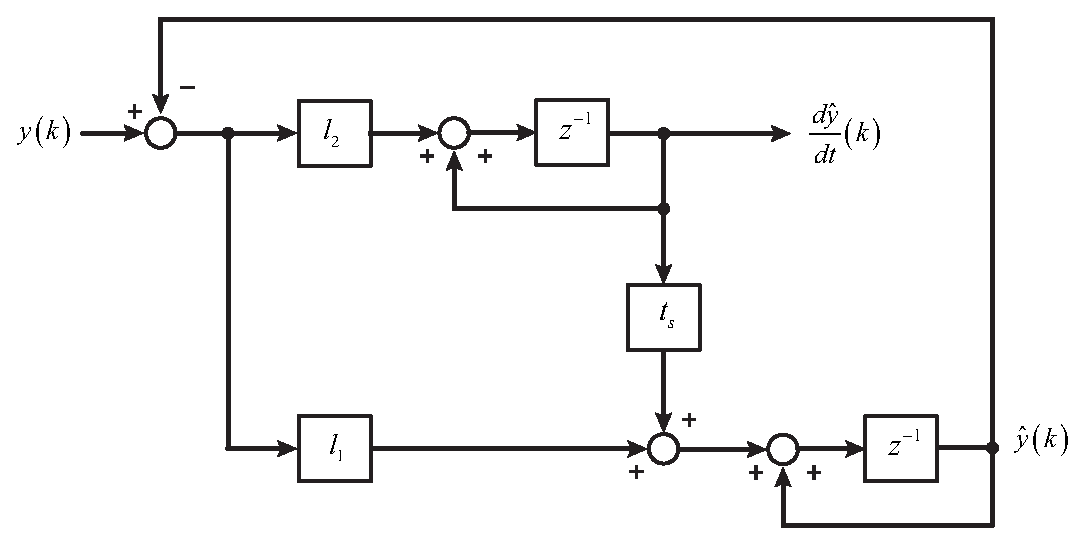
\includegraphics[width = 340pt, keepaspectratio] 
	{figures/double_integrator_observer_dt.eps}
	\captionsetup{width=0.5\textwidth, font=small}		
	\caption{Double Integrator Observer in Discrete Time Domain.}
	\label{}
\end{figure}
The above example shows how to implement a derivative block by an double 
integrator observer. The use of the observer as derivative is often used in 
practical implementation.

Let's now consider the case of derivative of a rotating phase signal generated 
by the function $\vartheta(t)=\atantwo(y(t),x(t))$ where
\begin{equation}
	\left\lbrace \begin{aligned}
	&	x(t)=\cos(\omega t) \\[6pt]		
	&	y(t)=\cos(\omega t)
	\end{aligned}\right. 
\end{equation}
and 
\begin{equation}
	\vartheta(t)=\atantwo(y(t),x(t))
\end{equation}
the variable $\vartheta(t)$ is a saw-tooth curve bonded between $-\pi$ to 
$\pi$;
\begin{figure}[H]
	\centering
	\includegraphics[width = 275pt, keepaspectratio] 
	{figures/double_integrator.eps}
	\captionsetup{width=0.5\textwidth, font=small}		
	\caption{Phase generation.}
	\label{}
\end{figure}
\noindent A way to emulate the image (or codomain) of $\atantwo()$ is the 
following 
function
\begin{equation}
	\vartheta(t)=-\pi+\bmod(\omega t+3\pi,2\pi)
\end{equation}
\begin{figure}[H]
	\centering
	\includegraphics[width = 440pt, keepaspectratio] 
	{figures/double_integrator_observer_dt_theta.eps}
	\captionsetup{width=0.5\textwidth, font=small}		
	\caption{Double Integrator Observer in Discrete Time Domain with bounder 
	block.}
	\label{}
\end{figure}
\noindent here some simulation results
	\begin{figure}[H]
	\centering
	\begin{subfigure}{.5\textwidth}
		\centering
		\includegraphics[width = 200pt, 
		keepaspectratio]{figures/double_integrator/double_integrator_theta.eps}
		\captionsetup{width=0.75\textwidth}		
		\caption{Phase $\vartheta(t)+w(t)$, where $w(t)$ is white noise, and 
		estimated phase $\hat{\vartheta}(t)$}
		\label{}
	\end{subfigure}%
	\begin{subfigure}{.5\textwidth}
		\centering
		\includegraphics[width = 200pt, 
		keepaspectratio]{figures/double_integrator/double_integrator_omega.eps}
		\captionsetup{width=0.75\textwidth}		
		\caption{Speed $\omega(t)$ and estimated speed $\hat{\omega}(t)$}
		\label{}
	\end{subfigure}		
	\captionsetup{width=0.5\textwidth, font=small}		
	\caption{Double integrator observer used as derivative applied to a 
	rotating phase signal.}
	\label{}
\end{figure}

$\triangleleft$ 
\end{example}

\section{State Feedback with Integrator}
\subsection{Continuous-time Domain Case}
The following control architecture is useful when it is required to track a 
given constant reference with zero steady state error.

The basic principle of the pole placement (or state feedback) with integrator 
is to insert an integrator in the feed-forward path between the error 
comparator and the plant, as shown in Figure~\ref{figure_servo_tc_1}.
\begin{figure}[H]
	\centering
	\includegraphics[width = 440pt, 
	keepaspectratio]{figures/servo_ct_3.eps}
	\captionsetup{width=0.5\textwidth, font=small}
	\caption{Servo system with state feedback and integral control - continuous 
		time case}
	\label{figure_servo_tc_1}
\end{figure}

\noindent\textbf{Considering SISO case.}

From figure \ref{figure_servo_tc_1} we can write the following equations:
\begin{equation}\label{eq_servo_ct_1}
	\begin{aligned}
		\dot{\vec{x}}(t) &= 
		\tilde{\mathbf{A}}\vec{x}(t)+\tilde{\mathbf{B}}{u}(t) \\[6pt]
		{y}(t) &= {\mathbf{C}}\vec{x}(t) \\[6pt]
		u(t) &= -{\mathbf{K}}\vec{x}(t) + k_i\xi \\[6pt]
		\dot{\xi}(t) &= r(t) - y(t) = r(t)-{\mathbf{C}}\vec{x}(t)
	\end{aligned}
\end{equation}
where $\vec{x}$ is the state vector of the plant.

We assume that $(\tilde{\mathbf{A}},\tilde{\mathbf{B}})$ is completely state 
controllable.
The set of equations reported in Eq.~\eqref{eq_servo_ct_1} cab be rewritten as 
follows
\begin{equation}\label{eq_servo_ct_2}
	\begin{bmatrix}
		\dot{\vec{x}}(t) \\[6pt] \dot{\xi}(t)
	\end{bmatrix} = 
	\begin{bmatrix}
		\tilde{\mathbf{A}} & \mathbf{0} \\[6pt]
		-{\mathbf{C}} & 0
	\end{bmatrix} 
	\begin{bmatrix}
		{\vec{x}}(t) \\[6pt] {\xi}(t)
	\end{bmatrix}+
	\begin{bmatrix}
		\tilde{\mathbf{B}} \\[6pt] 0
	\end{bmatrix}u(t)+
	\begin{bmatrix}
		{\mathbf{0}} \\[6pt] 1
	\end{bmatrix}r(t)
\end{equation}

The control problem we are considering is basically a tracking problem, that 
means we want to analyse the behaviour of the tracking error $r(t) - y(t)$, in 
particular we shall design an asymptotically stable system such that 
$\vec{x}_{\infty}$, $\xi_{\infty}$ and $y_{\infty}$ approach constant values 
respectively (we assume $r(t)=r_{\infty}$ is constant). Then, at steady state, 
we obtain that $\dot{\xi}(t)=0$, and results in $y_{\infty} = r_{\infty}$.
Notice that at steady state we have
\begin{equation}\label{eq_servo_ct_3}
	\begin{bmatrix}
		\dot{\vec{x}}_{\infty} \\[6pt] \dot{\xi}_{\infty}
	\end{bmatrix} = 
	\begin{bmatrix}
		\tilde{\mathbf{A}} & \mathbf{0} \\[6pt]
		-{\mathbf{C}} & 0
	\end{bmatrix} 
	\begin{bmatrix}
		{\vec{x}}_{\infty} \\[6pt] {\xi}_{\infty}
	\end{bmatrix}+
	\begin{bmatrix}
		\tilde{\mathbf{B}} \\[6pt] 0
	\end{bmatrix}u_{\infty}+
	\begin{bmatrix}
		{\mathbf{0}} \\[6pt] 1
	\end{bmatrix}r_{\infty}
\end{equation}
Noting, again, that $r(t)$ is a step input, we have $r(t)=r_{\infty} = r\ 
\text{(constant)}$ for $t > 0$. By subtracting Eq.~\eqref{eq_servo_ct_3} from 
Eq.~
\ref{eq_servo_ct_2}, we obtain
\begin{equation}\label{eq_servo_ct_4}
	\begin{bmatrix}
		\dot{\vec{x}}(t) - \dot{\vec{x}}_{\infty} \\[6pt] 
		\dot{\xi}(t)-\dot{\xi}_{\infty}
	\end{bmatrix} = 
	\begin{bmatrix}
		\tilde{\mathbf{A}} & \mathbf{0} \\[6pt]
		-{\mathbf{C}} & 0
	\end{bmatrix} 
	\begin{bmatrix}
		\vec{x}(t)-{\vec{x}}_{\infty} \\[6pt] {\xi}(t)-{\xi}_{\infty}
	\end{bmatrix}+
	\begin{bmatrix}
		\tilde{\mathbf{B}} \\[6pt] 0
	\end{bmatrix}
	\begin{bmatrix}
		u(t)-u_{\infty}
	\end{bmatrix}
\end{equation}
Define (we apply a change of variable in order to remove the steady state 
off-set)
\begin{equation}\label{eq_servo_ct_5}
	\begin{aligned}
		\vec{x}(t)-\vec{x}_{\infty} &= \Delta\vec{x}(t) \\[6pt]
		{\xi}(t)-{\xi}_{\infty} &= \Delta{\xi}(t) \\[6pt]
		{u}(t)-{u}_{\infty} &= \Delta u(t)
	\end{aligned}
\end{equation}
The Eq.~\eqref{eq_servo_ct_4} can be written as
\begin{equation}\label{eq_servo_ct_6}
	\begin{bmatrix}
		\Delta\dot{\vec{x}}(t) \\[6pt] \Delta\dot{\xi}(t)
	\end{bmatrix} = 
	\begin{bmatrix}
		\tilde{\mathbf{A}} & \mathbf{0} \\[6pt]
		-{\mathbf{C}} & 0
	\end{bmatrix} 
	\begin{bmatrix}
		\Delta\vec{x}(t)\\[6pt] \Delta{\xi}(t)
	\end{bmatrix}+
	\begin{bmatrix}
		\tilde{\mathbf{B}} \\[6pt] 0
	\end{bmatrix}
	\begin{bmatrix}
		\Delta u(t)
	\end{bmatrix}
\end{equation}
where
\begin{equation}\label{eq_servo_ct_7}
	\Delta u(t)  = -{\mathbf{K}}\Delta\vec{x}(t) + k_i\Delta\xi(t)
\end{equation}
The change of variable of Eq.\eqref{eq_servo_ct_5} permit to convert a tracking problem into a regulation problem, that means the control problem reduces to find $\mathbf{K}$ and $k_i$ such that 
\begin{flalign}\label{eq_servo_ct_7b}
	&\Delta\vec{x}(t) \xrightarrow[t\rightarrow\infty]{} 0 \\[6pt]
	& \Delta{\xi}(t) \xrightarrow[t\rightarrow\infty]{} 0 \\[6pt]
	& \Delta u(t) \xrightarrow[t\rightarrow\infty]{} 0
\end{flalign}

Define a new $(n+1)$th-order error vector $\vec{e}(t)$ by 
\begin{equation*}\label{eq_servo_ct_8}
	\vec{e}(t)  = 
	\begin{bmatrix}
		\Delta\vec{x}(t) \\[6pt] \Delta\xi(t)
	\end{bmatrix} = (n+1)\text{-vector}
\end{equation*}
Then Eq. \ref{eq_servo_ct_6} becomes
\begin{equation}\label{eq_servo_ct_9}
	\dot{\vec{e}}(t) = \tilde{\mathbf{A}}'\ \vec{e}(t) + \tilde{\mathbf{B}}'\ 
	\Delta u(t)
\end{equation}
where
\begin{equation}\label{eq_servo_ct_10}
	\tilde{\mathbf{A}}'  = 
	\begin{bmatrix}
		\tilde{\mathbf{A}} & \mathbf{0} \\[6pt]
		-{\mathbf{C}} & 0
	\end{bmatrix}, \quad
	\tilde{\mathbf{B}}'  = 
	\begin{bmatrix}
		\tilde{\mathbf{B}} \\[6pt] 0
	\end{bmatrix}
\end{equation}
and Eq.~\eqref{eq_servo_ct_7} becomes
\begin{equation}\label{eq_servo_ct_11}
	\begin{aligned}
		\Delta u(t) &= -{\mathbf{K}}'\ \vec{e}(t) \\[6pt]
		&= \begin{bmatrix}
			{\mathbf{K}} & -k_i
		\end{bmatrix} \begin{bmatrix}
			\Delta\vec{x}(t) \\[6pt] \Delta\xi(t)
		\end{bmatrix}  \\[6pt]
		&= -{\mathbf{K}}\Delta\vec{x}(t) + k_i\Delta\xi(t)
	\end{aligned}
\end{equation}
where
\begin{equation}\label{eq_servo_ct_12}
	{\mathbf{K}}'= \begin{bmatrix}
		{\mathbf{K}} & -k_i
	\end{bmatrix}
\end{equation}

The dynamic of the state vector $\vec{e}(t)$ can be computed by the 
Eq.~\eqref{eq_servo_ct_13} which can be obtained by substituting 
Eq.~\eqref{eq_servo_ct_11} into Eq.~\eqref{eq_servo_ct_9}, as follows
\begin{equation}\label{eq_servo_ct_13}
	\dot{\vec{e}}(t) = \left(\tilde{\mathbf{A}}' - 
	\tilde{\mathbf{B}}'\tilde{\mathbf{K}}'\right)\vec{e}(t)
\end{equation}
where ${\mathbf{K}}'$ can be computed by poles placement.

\vspace{5mm}
\begin{mybox}
	\textbf{The design of the state feedback with integrator, in the 
		continuous-time domain, reduces to the pole-placement problem:} 
	\begin{equation}\label{eq_servo_ct_14a}
		\Bigg|s\mathbf{I}-\Big(\tilde{\mathbf{A}}' - 
		\tilde{\mathbf{B}}'\tilde{\mathbf{K}}'\Big)\Bigg|=\sum_{k=1}^{n}(s-\mu_k)
	\end{equation}
	where
	\begin{equation}\label{eq_servo_ct_14b}
		{\mathbf{K}}'= \begin{bmatrix}
			{\mathbf{K}} & -k_i
		\end{bmatrix}
	\end{equation}
	and
	\begin{equation}\label{eq_servo_ct_15}
		\tilde{\mathbf{A}}'  = 
		\begin{bmatrix}
			\tilde{\mathbf{A}} & \mathbf{0} \\[6pt]
			-{\mathbf{C}} & 0
		\end{bmatrix}, \quad
		\tilde{\mathbf{B}}'  = 
		\begin{bmatrix}
			\tilde{\mathbf{B}} \\[6pt] 0
		\end{bmatrix}
	\end{equation}
\end{mybox}

\subsection{Discrete-time Representation of an Integrator}
This subsection wants to describe how to represent an integrator operator in 
discrete time domain. At this aim the discretization of a PI control is 
proposed. The method which will be used is not the classical which can be find 
in literature, but it will give a kind of continuity with the tools up to now 
described.

Figure~\ref{pi_continuous} shows the typical control architecture of a PI 
controller applied to a generic \textit{Plant}.
\begin{figure}[H]
	\centering
	\includegraphics[width = 400pt, 
	keepaspectratio,angle=0]{figures/pi_discrete/pi_continuous_1.eps}
	\captionsetup{width=0.5\textwidth, font=small}
	\caption{PI-controller architecture in continuous time domain.}
	\label{pi_continuous}
\end{figure}
Mathematically speaking the control structure of Figure~\ref{pi_continuous} can 
be represented as follows
\begin{flalign}
	\Delta y(t) &= y^{ref}(t)-y(t) \label{pi_integrator_eq0} \\[6pt]
	u(t) &= u_p(t) + u_i(t) \\[6pt]
	u_p(t) &= k_p \Delta y(t) \\[6pt]
	\dot{u}_i(t) &= k_i \Delta y(t) \label{pi_integrator_eq1}
\end{flalign}
Eq.~\eqref{pi_integrator_eq1} can be correlated to the canonical representation 
of a linear system as follows
\begin{flalign}\label{pi_integrator_eq2}
	\dot{u}_i(t)=\tilde{\mathbf{A}}u_i(t) + \tilde{\mathbf{B}} \Delta y(t)
\end{flalign}
where
\begin{flalign}
	\tilde{\mathbf{A}} &= 0 \\[6pt]	
	\tilde{\mathbf{B}} &= k_i
\end{flalign}
Now the discrete time representation of Eq.~\eqref{pi_integrator_eq2} can be 
computed applying the equations
\begin{flalign}
	\mathbf{A} &= e^{\tilde{\mathbf{A}}t_s} \label{pi_integrator_eq3}
	\\[6pt] 
	\mathbf{B} &= \int_{0}^{t_s}e^{\tilde{\mathbf{A}}\tau} 
	\tilde{\mathbf{B}}d\tau \label{pi_integrator_eq4}
\end{flalign}
which results in
\begin{flalign}\label{}
	{u}_i(k+1)={\mathbf{A}}u_i(k) + {\mathbf{B}} \Delta y(k)
\end{flalign}
where
\begin{flalign}
	\mathbf{A} &= e^{\tilde{\mathbf{A}}t_s} = 1 \label{pi_integrator_eq5} && 
	\\[6pt] 
	\mathbf{B} &= \int_{0}^{t_s}e^{\tilde{\mathbf{A}}\tau} 
	\tilde{\mathbf{B}}d\tau = k_it_s\label{pi_integrator_eq6} &&
\end{flalign}
Hence Eqs.~\eqref{pi_integrator_eq0}-~\eqref{pi_integrator_eq1} becomes
\begin{flalign}
	\Delta y(k) &= y^{ref}(k)-y(k) \label{pi_integrator_eq7} \\[6pt]
	u(k) &= u_p(k) + u_i(k) \\[6pt]
	u_p(k) &= k_p \Delta y(k) \\[6pt]
	{u}_i(k+1) &= 	{u}_i(k) + k_i t_s \Delta y(k) \label{pi_integrator_eq8}
\end{flalign}
as shown in Figure~\ref{pi_discrete_1}
\begin{figure}[H]
	\centering
	\includegraphics[width = 400pt, 
	keepaspectratio,angle=0]{figures/pi_discrete/pi_discrete_1.eps}
	\captionsetup{width=0.5\textwidth, font=small}
	\caption{PI-controller architecture in discrete time domain.}
	\label{pi_discrete_1}
\end{figure}
In some application Eq.~\eqref{pi_integrator_eq8} can also be represented as 
follows
\begin{flalign}
	{u}_i(k) &= {u}_i(k-1) + k_i t_s \Delta y(k)
\end{flalign}
as shown in Figure~\ref{pi_discrete_2}
\begin{figure}[H]
	\centering
	\includegraphics[width = 400pt, 
	keepaspectratio,angle=0]{figures/pi_discrete/pi_discrete_2.eps}
	\captionsetup{width=0.5\textwidth, font=small}
	\caption{PI-controller architecture in discrete time domain - alternative 
		representation.}
	\label{pi_discrete_2}
\end{figure}

\subsection{Discrete-time Domain Case}
A control system in which the output must follow a reference signals is called a 
\textit{servo system}, that means a servo system problem is a \textit{tracking problem}. In a servo, it is generally required that the system have one or more integrators within the closed loop to eliminate the 
steady state error. One way to introduce an integrator in the mathematical model of the closed loop system is to introduce a new state vector that integrates the difference between the reference vector $\vec{r}$ and the output vector $\vec{y}$. Figure~\ref{figure_servo_1} shows a possible block diagram 
configuration for a servo system with state feedback and integral control. The 
integrator can be included as part of the pole placement formulation.
\begin{figure}[H]
	\centering
	\includegraphics[width = 400pt, 
	keepaspectratio,angle=0]{figures/servo_1.eps}
	\captionsetup{width=0.5\textwidth, font=small}
	\caption{Servo system with state feedback and integral control}
	\label{figure_servo_1}
\end{figure}
Considering the following state and output equation
\begin{equation}\label{eq_servo_1}
	\begin{aligned}
		\vec{x}(k+1) &= \mathbf{A}\vec{x}(k)+\mathbf{B}\vec{u}(k) \\[6pt]
		\vec{y}(k) &= \mathbf{C}\vec{x}(k)
	\end{aligned}
\end{equation}
where
\begin{equation*}
	\begin{aligned}
		\vec{x}(k) &= \text{plant state vector ($n$-vector)}\\[6pt]
		\vec{u}(k) &= \text{control vector ($m$-vector)}\\[6pt]
		\vec{y}(k) &= \text{output vector ($m$-vector)}\\[6pt]
		\mathbf{A} &= \text{$n \times n$ matrix}\\[6pt]
		\mathbf{B} &= \text{$n \times m$ matrix}\\[6pt]
		\mathbf{C} &= \text{$m \times n$ matrix}
	\end{aligned}
\end{equation*}
The integrator state equation is
\begin{equation}\label{eq_servo_2}
	\begin{aligned}
		\vec{v}(k) = \mathbf{K}_I\left[ 
		\vec{r}(k)-\vec{y}(k)\right]+\vec{v}(k-1) 
	\end{aligned}
\end{equation}
where 
\begin{equation}
	\begin{aligned}
		\vec{v}(k) &= \text{actuating error vector ($m$-vector)}\\[6pt]
		\vec{r}(k) &= \text{command input vector ($m$-vector)}
	\end{aligned}
\end{equation}
Eq.~\eqref{eq_servo_2} can be rewritten as follows:
\begin{equation}\label{eq_servo_3}
	\begin{aligned}
		\vec{v}(k+1) = \mathbf{K}_I\left[ 
		\vec{r}(k+1)-\vec{y}(k+1)\right]+\vec{v}(k) 
	\end{aligned}
\end{equation}
In steady state conditions which means 
$\vec{v}(k+1)=\vec{v}(k)=\vec{v}_{\infty}$ Eq.~\eqref{eq_servo_3} reduces to 
\begin{equation}\label{eq_servo_4}
	\begin{aligned}
		\vec{r}(t) - \vec{y}_{\infty} =\vec{r}_{\infty} - \vec{y}_{\infty} = 0
	\end{aligned}
\end{equation}
The control vector $\vec{u}(k)$ is given by 
\begin{equation}
	\left\lbrace 
	\begin{aligned}
		\vec{v}(k) &= \mathbf{K}_I\left[ 
		\vec{r}(k)-\vec{y}(k)\right]+\vec{v}(k-1) \\[6pt]
		\vec{u}(k) &= -\mathbf{K}_x\vec{x}(k)+\vec{v}(k) 
	\end{aligned}
	\right. 
\end{equation}
or
\begin{equation}\label{eq_servo_5}
	\left\lbrace 
	\begin{aligned}
		\vec{v}(k+1) &= \mathbf{K}_I\left[ 
		\vec{r}(k+1)-\vec{y}(k+1)\right]+\vec{v}(k) \\[6pt]
		\vec{u}(k+1) &= -\mathbf{K}_x\vec{x}(k+1)+\vec{v}(k+1) 
	\end{aligned}
	\right. 
\end{equation}
Our design parameters are matrices $\mathbf{K}_x$ and $\mathbf{K}_I$.
In what follows we shall discuss the procedure for determining matrices 
$\mathbf{K}_x$ and $\mathbf{K}_I$.

The system dynamics may hence be described as follows
\begin{equation}\label{eq_servo_6}
	\begin{aligned}
		\vec{x}(k+1) = \mathbf{A}\vec{x}(k)+\mathbf{B}\vec{u}(k) = 
		\mathbf{A}\vec{x}(k)+\mathbf{B}\left[ 
		\vec{v}(k)-\mathbf{K}_x\vec{x}(k)\right] 
	\end{aligned}
\end{equation}
and the integral term as follows
\begin{equation}\label{eq_servo_7}
	\begin{aligned}
		\vec{v}(k+1) &= 
		\mathbf{K}_I\Big[\vec{r}(k+1)-\vec{y}(k+1)\Big]+\vec{v}(k)= \\[6pt]  
		&= 
		\mathbf{K}_I\Big[\vec{r}(k+1)-\mathbf{C}\vec{x}(k+1)\Big]+\vec{u}(k)+\mathbf{K}_x\vec{x}(k)=
		\\[6pt]
		&= \mathbf{K}_I\Big[\vec{r}(k+1)-\mathbf{C} \Big( 
		\mathbf{A}\vec{x}(k)+\mathbf{B}\vec{u}(k) \Big)  
		\Big]+\vec{u}(k)+\mathbf{K}_x\vec{x}(k)= \\[6pt]
		&= \Big[\mathbf{I}_m - \mathbf{K}_I\mathbf{C}\mathbf{B} \Big] 
		\vec{u}(k) + \Big[\mathbf{K}_x 
		-\mathbf{K}_I\mathbf{C}\mathbf{A}\Big] \vec{x}(k) + 
		\mathbf{K}_I\vec{r}(k+1)
	\end{aligned}
\end{equation}
but $\vec{v}(k+1)=\vec{u}(k+1)+\mathbf{K}_x\vec{x}(k+1)$ or
\begin{equation}
	\begin{aligned}
		\vec{u}(k+1) &= \vec{v}(k+1) - \mathbf{K}_x\vec{x}(k+1)  \\[6pt]
		&= \vec{v}(k+1) - \mathbf{K}_x\Big[\mathbf{A}\vec{x}(k)+\mathbf{B}\vec{u}(k)\Big] \\[6pt]
		&= \Big[\mathbf{I}_m - \mathbf{K}_I\mathbf{C}\mathbf{B} \Big] 
		\vec{u}(k) + \Big[\mathbf{K}_x 
		-\mathbf{K}_I\mathbf{C}\mathbf{A}\Big] \vec{x}(k) - \mathbf{K}_x\Big[\mathbf{A}\vec{x}(k)+\mathbf{B}\vec{u}(k)\Big] \\[6pt]
		&\qquad+ \mathbf{K}_I\vec{r}(k+1)
	\end{aligned}
\end{equation}
hence 
\begin{equation}\label{eq_servo_8}
	\begin{aligned}
		\vec{u}(k+1) &= 
		\Big[\mathbf{I}_m-\mathbf{K}_x\mathbf{B}-\mathbf{K}_I\mathbf{C}\mathbf{B}
		\Big] \vec{u}(k) + \\[6pt]
		&\qquad+\Big[\mathbf{K}_x - 
		\mathbf{K}_x\mathbf{A}-\mathbf{K}_I\mathbf{C}\mathbf{A} \Big] 
		\vec{x}(k) + \\[6pt]
		&\qquad+  \mathbf{K}_I\vec{r}(k+1)
	\end{aligned}
\end{equation}
Eq.~\eqref{eq_servo_8} describes the evolution of the control input $\vec{u}(k+1)$ as function previous control input $\vec{u}(k)$ and by the state vector $\vec{x}(k)$, removing any relation with the integral corrective term $\vec{v}(k)$.

Combining $\vec{x}(k+1)$ and $\vec{u}(k+1)$ in matrix form we obtain
\begin{equation}\label{eq_servo_9}
	\begin{aligned}
		\begin{bmatrix}
			\vec{u}(k+1) \\[6pt]  
			\vec{x}(k+1)
		\end{bmatrix} &=
		\begin{bmatrix}
			\mathbf{I}_m-\mathbf{K}_x\mathbf{B}-\mathbf{K}_I\mathbf{C}\mathbf{B}
			&  \mathbf{K}_x-\mathbf{K}_x\mathbf{A} 
			-\mathbf{K}_I\mathbf{C}\mathbf{A} \\[6pt]
			\mathbf{B} & \mathbf{A}
		\end{bmatrix}
		\begin{bmatrix}
			\vec{u}(k) \\[6pt]  
			\vec{x}(k)
		\end{bmatrix} + \\[6pt]
		&+
		\begin{bmatrix}
			\mathbf{K}_I \\[6pt]  
			\mathbf{0}
		\end{bmatrix}\vec{r}(k+1) \\[6pt]  
		\vec{y}(k) &= 
		\begin{bmatrix}
			0 & \mathbf{C}
		\end{bmatrix}
		\begin{bmatrix}
			\vec{u}(k) \\[6pt]  
			\vec{x}(k)
		\end{bmatrix}
	\end{aligned}
\end{equation}
Note that the closed loop poles of the system are determined by the system 
itself and do not depend on the command input $\vec{r}(k)$. The eigenvalues of 
the state matrix in Eq.~\eqref{eq_servo_9} determine the closed loop poles of 
the 
system.
In order to apply the pole placement technique to the design of the servo 
system, consider the case where the command vector $\vec{r}(k)$ is constant 
$\vec{r}(k) \rightarrow\vec{r}$, hence, Eq.~\eqref{eq_servo_9} become
\begin{equation}\label{eq_servo_10}
	\begin{aligned}
		\begin{bmatrix}
			\vec{u}(k+1) \\[6pt]  
			\vec{x}(k+1)
		\end{bmatrix} &=
		\begin{bmatrix}
			\mathbf{I}_m-\mathbf{K}_x\mathbf{B}-\mathbf{K}_I\mathbf{C}\mathbf{B}
			&  
			\mathbf{K}_x-\mathbf{K}_x\mathbf{A}-\mathbf{K}_I\mathbf{C}\mathbf{A}\\[6pt]
			
			\mathbf{B} & \mathbf{A}
		\end{bmatrix}
		\begin{bmatrix}
			\vec{u}(k) \\[6pt]  
			\vec{x}(k)
		\end{bmatrix} + \\[6pt]
		&+
		\begin{bmatrix}
			\mathbf{K}_I\vec{r} \\[6pt]  
			\mathbf{0}
		\end{bmatrix}
	\end{aligned}
\end{equation}
In steady state conditions the quantities $\vec{x}(k)$, $\vec{u}(k)$ and 
$\vec{v}(k)$ tend to constant value as 
\begin{equation}
	\begin{aligned}
		&\vec{x}(k)\rightarrow\vec{x}_{\infty} \\[6pt]
		&\vec{u}(k)\rightarrow\vec{u}_{\infty} \\[6pt]
		&\vec{v}(k)\rightarrow\vec{v}_{\infty}
	\end{aligned}
\end{equation}
respectively. Thus from Eq.~\eqref{eq_servo_2} we obtain the following equation 
at steady state
\begin{equation}
	\begin{aligned}
		\vec{v}_{\infty} = \vec{v}_{\infty} +\vec{r}-\vec{y}_{\infty}
	\end{aligned}
\end{equation}
There is no steady state error in the output when the command input is a step 
vector. Hence Eq.~\eqref{eq_servo_10} becomes
\begin{equation}\label{eq_servo_11}
	\begin{aligned}
		\begin{bmatrix}
			\vec{u}_{\infty} \\[6pt]  
			\vec{x}_{\infty}
		\end{bmatrix} &=
		\begin{bmatrix}
			\mathbf{I}_m-\mathbf{K}_x\mathbf{B}-\mathbf{K}_I\mathbf{C}\mathbf{B}
			&  
			\mathbf{K}_x-\mathbf{K}_x\mathbf{A}-\mathbf{K}_I\mathbf{C}\mathbf{A}\\[6pt]
			
			\mathbf{B} & \mathbf{A}
		\end{bmatrix}
		\begin{bmatrix}
			\vec{u}_{\infty} \\[6pt]  
			\vec{x}_{\infty}
		\end{bmatrix} + \\[6pt]
		&+
		\begin{bmatrix}
			\mathbf{K}_I\vec{r} \\[6pt]  
			\mathbf{0}
		\end{bmatrix}
	\end{aligned}
\end{equation}
Let us define the error vectors by
\begin{equation}\label{from_track_to_reg}
	\begin{aligned}
		\Delta\vec{x}(k) &= \vec{x}(k)-\vec{x}_{\infty} \\[6pt]
		\Delta\vec{u}(k) &= \vec{u}(k)-\vec{u}_{\infty}
	\end{aligned}
\end{equation}
Again by applying Eq.~\eqref{from_track_to_reg} a tracking problem is reduced to a regulation problem, where 
\begin{flalign}\label{eq_servo_ct_7b}
	&\Delta\vec{x}(k) \xrightarrow[k\rightarrow\infty]{} \vec{0} \\[6pt]
	& \Delta \vec{u}(k) \xrightarrow[k\rightarrow\infty]{} \vec{0}
\end{flalign}

Then subtracting Eq.~\eqref{eq_servo_11} from Eq.~\eqref{eq_servo_10} we obtain
\begin{equation}\label{eq_servo_12}
	\begin{aligned}
		\begin{bmatrix}
			\Delta\vec{u}(k+1) \\[6pt]  
			\Delta\vec{x}(k+1)
		\end{bmatrix} &=
		\begin{bmatrix}
			\mathbf{I}_m-\mathbf{K}_x\mathbf{B}-\mathbf{K}_I\mathbf{C}\mathbf{B}
			&  
			\mathbf{K}_x-\mathbf{K}_x\mathbf{A}-\mathbf{K}_I\mathbf{C}\mathbf{A}\\[6pt]
			
			\mathbf{B} & \mathbf{A}
		\end{bmatrix}
		\begin{bmatrix}
			\Delta\vec{u}(k) \\[6pt]  
			\Delta\vec{x}(k)
		\end{bmatrix}
	\end{aligned}
\end{equation}\\
The dynamics of the system are determined by the eigenvalues of the state 
matrix appearing in Eq.~\eqref{eq_servo_12}. Eq~\eqref{eq_servo_12} can be 
modified as following
\begin{equation}\label{eq_servo_13}
	\begin{aligned}
		\begin{bmatrix}
			\Delta\vec{u}(k+1) \\[6pt]  
			\Delta\vec{x}(k+1)
		\end{bmatrix} =
		\underbrace{\begin{bmatrix}
				\mathbf{0} & \mathbf{0} \\[6pt]  
				\mathbf{B} & \mathbf{A}
		\end{bmatrix}}_{\mathbf{A'}}
		\begin{bmatrix}
			\Delta\vec{u}(k) \\[6pt]  
			\Delta\vec{x}(k)
		\end{bmatrix}+
		\underbrace{\begin{bmatrix}
				\mathbf{I}_m \\[6pt]  
				\mathbf{0}
		\end{bmatrix}}_{\mathbf{B'}}\vec{w}(k)
	\end{aligned}
\end{equation}
where 
\begin{equation}\label{eq_servo_14}
	\begin{aligned}
		\vec{w}(k) = 
		\begin{bmatrix}
			\mathbf{I}_m-\mathbf{K}_x\mathbf{B}-\mathbf{K}_I\mathbf{C}\mathbf{B}
			&  
			\mathbf{K}_x-\mathbf{K}_x\mathbf{A}-\mathbf{K}_I\mathbf{C}\mathbf{A}
		\end{bmatrix}
		\begin{bmatrix}
			\Delta\vec{u}(k) \\[6pt]  
			\Delta\vec{x}(k)
		\end{bmatrix}
	\end{aligned}
\end{equation}
If we define 
\begin{equation*}
	\begin{aligned}
		\vec{\xi}(k) &= 
		\begin{bmatrix}
			\Delta\vec{u}(k) \\[6pt]  
			\Delta\vec{x}(k)
		\end{bmatrix} = \text{$(n+m)$-vector} \\[6pt]
		\mathbf{A'} &= 
		\begin{bmatrix}
			\mathbf{0} & \mathbf{0} \\[6pt]  
			\mathbf{B} & \mathbf{A}
		\end{bmatrix} = \text{$(n+m)\times(n+m)$ matrix} \\[6pt]
		\mathbf{B'} &= 
		\begin{bmatrix}
			\mathbf{I}_m \\[6pt]  
			\mathbf{0}
		\end{bmatrix}= \text{$(n+m)\times m$ matrix} \\[6pt] 
		\mathbf{K'} &= -
		\begin{bmatrix}
			\mathbf{I}_m-\mathbf{K}_x\mathbf{B}-\mathbf{K}_I\mathbf{C}\mathbf{B}
			&  
			\mathbf{K}_x-\mathbf{K}_x\mathbf{A}-\mathbf{K}_I\mathbf{C}\mathbf{A}
		\end{bmatrix}= \text{$m \times (n+m)$ matrix} \\[6pt] 
	\end{aligned}
\end{equation*}
The Eq.~\eqref{eq_servo_13} and~\eqref{eq_servo_14} become, respectively
\begin{equation}\label{eq_servo_15}
	\begin{aligned}
		\vec{\xi}(k+1) &= \mathbf{A'}\vec{\xi}+\mathbf{B'}\vec{w}(k) \\[6pt] 
		\vec{w}(k) &= -\mathbf{K'}\vec{\xi}(k)
	\end{aligned}
\end{equation}
Once the desired closed loop poles are specified, matrix $\mathbf{K'}$ can be 
determined by the pole placement technique, e.g. by use of Ackermann's formula
\begin{equation*}
	\begin{aligned}
		\mathbf{K'} &= \begin{bmatrix} 0&0&...&0&1 \end{bmatrix} 
		\mathbf{M'}^{-1}q(\mathbf{A'}) \\[6pt]
		\mathbf{M'} &= \begin{bmatrix} 
			\mathbf{B'}&\mathbf{A'}\mathbf{B'}&...&\left( \mathbf{A'}\right) 
			^{n+m-1}\mathbf{B'} \end{bmatrix}
	\end{aligned}
\end{equation*}
Once matrix $\mathbf{K'}$ is derived via pole placement or other methods, the matrices $\mathbf{K}_x$ and 
$\mathbf{K}_I$ can be obtained as follows.

Note that
\begin{equation}
	\begin{aligned}
		\begin{bmatrix} 
			\mathbf{K}_I & \mathbf{K}_x
		\end{bmatrix}
		\begin{bmatrix} 
			\mathbf{C}\mathbf{B} & \mathbf{C}\mathbf{A} \\[6pt] 
			\mathbf{B} & \mathbf{A}-\mathbf{I}_n
		\end{bmatrix} &=
		\begin{bmatrix} 
			\mathbf{K}_x\mathbf{B} +\mathbf{K}_I\mathbf{C}\mathbf{B} & 
			-\mathbf{K}_x+\mathbf{K}_x\mathbf{A}+\mathbf{K}_I\mathbf{C}\mathbf{A}\end{bmatrix}
		= \\[6pt] 
		&=\mathbf{K'} + \begin{bmatrix} 
			\mathbf{I}_m & \mathbf{0}
		\end{bmatrix}
	\end{aligned}
\end{equation}
the desired gain matrices $		\begin{bmatrix} \mathbf{K}_I & \mathbf{K}_x \end{bmatrix}$ may be calculated according to
\begin{equation}
	\begin{aligned}
		\begin{bmatrix} 
			\mathbf{K}_I & \mathbf{K}_x
		\end{bmatrix} = \left\lbrace \mathbf{K'}+
		\begin{bmatrix} 
			\mathbf{I}_m & \mathbf{0}
		\end{bmatrix}\right\rbrace 
		\begin{bmatrix} 
			\mathbf{C}\mathbf{B} & \mathbf{C}\mathbf{A} \\[6pt] 
			\mathbf{B} & \mathbf{A}-\mathbf{I}_n
		\end{bmatrix}^{-1}
	\end{aligned}
\end{equation}

\vspace{5mm}
\begin{mybox}
	\textbf{The design of state feedback with integrator, in the discrete-time 
		domain, reduces to a pole placement problem applied to the state feedback system}
	\begin{flalign}
		\vec{\xi}(k+1) &= \mathbf{A'}\vec{\xi}+\mathbf{B'}\vec{w}(k) \\[6pt] 
		\vec{w}(k) &= -\mathbf{K'}\vec{\xi}(k)
	\end{flalign}
	where
	\begin{equation}
		\begin{aligned}
			\mathbf{A'} &= 
			\begin{bmatrix}
				\mathbf{0} & \mathbf{0} \\[6pt]  
				\mathbf{B} & \mathbf{A}
			\end{bmatrix}, \quad
			\mathbf{B'} &= 
			\begin{bmatrix}
				\mathbf{I}_m \\[6pt]  
				\mathbf{0}
			\end{bmatrix},	\quad
			\vec{\xi}(k) &= 
			\begin{bmatrix}
				\Delta\vec{u}(k) \\[6pt]  
				\Delta\vec{x}(k)
			\end{bmatrix}	
		\end{aligned}
	\end{equation}
	In particular, the control problem, reduces to the derivation of the preliminary state feedback matrix $\mathbf{K'}$ by pole placement or other techniques like linear quadratic regulator, e.g.
	%\begin{equation}
	%	\begin{aligned}
		%		&\texttt{[Klqr] = lqr(A,B,Q,R)} \\[6pt]
		%		&\texttt{[Klqr] = dlqr(Ad,Bd,Q,R)}
		%	\end{aligned}
	%\end{equation}
	\begin{equation}
		\texttt{[K'] = dlqr(A',B',Q,R)}
	\end{equation} 
	or
	\begin{equation}
		\texttt{[K'] = acker(A',B',[zpoles])}
	\end{equation} 
	Once the matrix gain $\mathbf{K'}$ is calculated the effective state feedback 
	matrix $\begin{bmatrix} \mathbf{K}_I & \mathbf{K}_x \end{bmatrix}$ can be derived by the transformation
	\begin{equation}
		\begin{aligned}
			\begin{bmatrix} 
				\mathbf{K}_I & \mathbf{K}_x
			\end{bmatrix} = \left\lbrace \mathbf{K'}+
			\begin{bmatrix} 
				\mathbf{I}_m & \mathbf{0}
			\end{bmatrix}\right\rbrace 
			\begin{bmatrix} 
				\mathbf{C}\mathbf{B} & \mathbf{C}\mathbf{A} \\[6pt] 
				\mathbf{B} & \mathbf{A}-\mathbf{I}_n
			\end{bmatrix}^{-1}
		\end{aligned}
	\end{equation}
\end{mybox}

\vspace{5mm}
\noindent\textbf{State observer inclusion}. When state vector is not 
measurable, condition which frequently occur, the use of a state observer is 
necessary. Figure~\ref{figure_servo_2} shows a possible architecture including 
in additional to the state feedback with integrator control, a state observer 
block.
\begin{figure}[H]
	\centering
	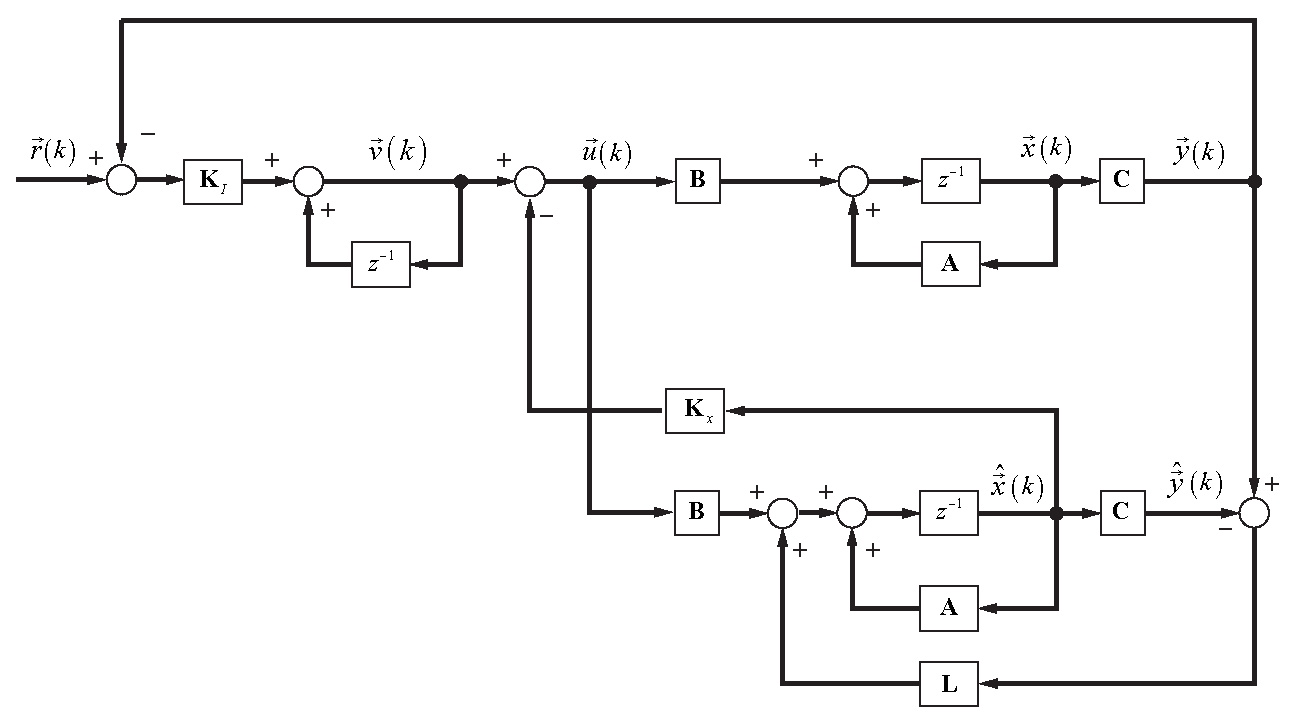
\includegraphics[width = 475pt, 
	keepaspectratio,angle=0]{figures/servo_2.eps}
	\captionsetup{width=0.5\textwidth, font=small}
	\caption{Servo system with observed state feedback and integral control}
	\label{figure_servo_2}
\end{figure}

The same considerations hold for the case SISO where $r(t)$, $y(t)$ and $v(t)$ are a scalars and $\mathbf{K}_I$ reduces to $k_i$, see also Figure~\ref{figure_servo_3} and Figure~\ref{figure_servo_4}

\begin{figure}[H]
	\centering
	\includegraphics[width = 475pt, 
	keepaspectratio,angle=0]{figures/servo_3.eps}
	\captionsetup{width=0.5\textwidth, font=small}
	\caption{Servo system with observed state feedback and integral control. SISO case.}
	\label{figure_servo_3}
\end{figure}
\begin{figure}[H]
	\centering
	\includegraphics[width = 475pt, 
	keepaspectratio,angle=0]{figures/servo_4.eps}
	\captionsetup{width=0.5\textwidth, font=small}
	\caption{Servo system with observed state feedback and integral control. SISO case.}
	\label{figure_servo_4}
\end{figure}

\chapter{Ljapunov Stability} 
This lecture covers some arguments regarding the Ljapunov stability and its 
application in design of control system. We start with an overview on phase 
portrait representation and after that, we will face up to the basic concept of 
Ljapunov's direct method applied to autonomous system. Main references are 
\cite{p27} and \cite{p28}.
\section{Some backgrounds} 
Consider the pendulum of Figure~\ref{pendulum2} 
\begin{figure}[H]
	\centering
	\includegraphics[width = 140pt, 
	keepaspectratio]{figures/ljapunov/pendulum2.eps}
	\captionsetup{width=0.75\textwidth}		
	\caption{Pendulum.}
	\label{pendulum2}
\end{figure}
Where the kinetic and potential energy can be expressed as follows 
\begin{equation*}
	E_{kin} = \frac{1}{2}ml^2\dot{\vartheta}^2
\end{equation*}
\begin{equation*}
	E_{pot} = mgl(1-\cos\vartheta)
\end{equation*}
Applying the Euler-Lagrange equation we obtain
\begin{equation*}
	\frac{d}{dt}\left(\frac{\partial E_{kin}}{\partial \dot{q}_i} \right) - 
	\frac{\partial E_{kin}}{\partial q_i} + \frac{\partial E_{pot}}{\partial 
	q_i} = Q_{diss}
\end{equation*}
where $Q_{diss} = -b\dot{\vartheta}$ which is a force due to the friction and 
results in the following second order differential equation
\begin{equation}
	ml^2\ddot{\vartheta} +mgl\sin\vartheta = -b\dot{\vartheta} 
\end{equation}
which in state space form results as follows
\begin{equation}
	\left\lbrace \begin{aligned}
		\dot{x}_1 &=  x_2 \\[6pt] 
		\dot{x}_2 &= -\frac{g}{l}\sin x_1 -\frac{b}{ml}x_2
	\end{aligned}\right. 
\end{equation}

Now we consider the case of small oscillation introducing the approximation 
$\sin\vartheta\approx\vartheta$ and we consider the case $b=0$ and $g=l$ which 
results in the following harmonic oscillator
\begin{equation}
	\begin{aligned}
		\begin{bmatrix} \dot{x}_1 \\ \dot{x}_2 \end{bmatrix} &= \begin{bmatrix} 
		0 & 1 \\ -1 & 0 \end{bmatrix} \begin{bmatrix} {x}_1 \\ {x}_2 
		\end{bmatrix} \\[6pt]
		\vec{x}(0) &= \begin{bmatrix} 1 & 0 \end{bmatrix}^T
	\end{aligned}
\end{equation}
where $\vec{x}(0)$ is the initial condition, $\mathbf{A} = \begin{bmatrix} 0 & 
1 \\ -1 & 0 \end{bmatrix}$ and $\vec{x}(t)= \begin{bmatrix} x_1(t) & x_2(t) 
\end{bmatrix}^T$.\\

The solution of the dynamical system is 
\begin{equation}
	\vec{x}(t) = e^{\mathbf{A}t}\vec{x}(0)
\end{equation}
and can be solved as follows
\begin{equation}
	\begin{aligned}
		\vec{x}(t) &= 
		\mathcal{L}^{-1}\Big\{\Big[s\mathbf{I}-\mathbf{A}\Big]^{-1}\Big\}\vec{x}(0)
		 = \mathcal{L}^{-1}\Big\{\frac{1}{s^2+1}\begin{bmatrix} s & 1 \\ -1 & s 
		\end{bmatrix}\Big\}\vec{x}(0) = \\[6pt]
		&= \begin{bmatrix} \cos(t) & \sin(t) \\ -\sin(t) & \cos(t) 
		\end{bmatrix}\vec{x}(0) = \begin{bmatrix} \cos(t) & -\sin(t) 
		\end{bmatrix}^T
	\end{aligned}
\end{equation}
The solution $\vec{x}(t) = \begin{bmatrix} x_1(t) & x_2(t) \end{bmatrix}^T = 
\begin{bmatrix} \cos(t) & -\sin(t) \end{bmatrix}^T$ can be plotted in the plane 
$\big(x_1 , x_2\big)$ - which is called \textit{phase-portrait}. The solution 
$\vec{x}(t)$ is the parametric representation of a circle with unitary radius. 
Selecting any initial condition different from zero, we can observe that the 
trajectory state vector is stationary - there isn't any loss of energy - and 
the motus is a periodic cycles as in a harmonic oscillator, see also 
Figure~\ref{armonic_oscillator}.
\begin{figure}[H]
	\centering
	\includegraphics[width = 300pt, 
	keepaspectratio]{figures/ljapunov/harmonic_oscillator.eps}
	\captionsetup{width=0.75\textwidth}		
	\caption{Phase portrait of the harmonic oscillator for different initial 
	conditions.}
	\label{armonic_oscillator}
\end{figure}

Consider now the damped version (with friction factor like $b=\frac{1}{2}$) of 
the harmonic oscillator 
\begin{equation}
	\begin{aligned}
		\begin{bmatrix} \dot{x}_1 \\ \dot{x}_2 \end{bmatrix} &= \begin{bmatrix} 
		0 & 1 \\ -1 & -\frac{1}{2} \end{bmatrix} \begin{bmatrix} {x}_1 \\ {x}_2 
		\end{bmatrix} \\[6pt]
		\vec{x}(0) &= \begin{bmatrix} 1 & 0 \end{bmatrix}^T
	\end{aligned}
\end{equation}
where $\vec{x}(0)$ is the initial condition and $\mathbf{A} = \begin{bmatrix} 0 
& 1 \\ -1 & -\frac{1}{2} \end{bmatrix}$ and $\vec{x}(t)= \begin{bmatrix} x_1(t) 
& x_2(t) \end{bmatrix}^T$.\\

The solution of the dynamical system is
\begin{equation}
	\vec{x}(t) = e^{\mathbf{A}t}\vec{x}(0)
\end{equation}
and can be solved as follows
\begin{equation}
	\begin{aligned}
		\vec{x}(t) &= 
		\mathcal{L}^{-1}\Big\{\Big[s\mathbf{I}-\mathbf{A}\Big]^{-1}\Big\}\vec{x}(0)
		 = \mathcal{L}^{-1}\Big\{\frac{1}{2s^2+s+2}\begin{bmatrix} 2s+1 & 2 \\ 
		-2 & 2s \end{bmatrix}\Big\}\vec{x}(0) = \\[6pt]
		&= \begin{bmatrix} e^{-\alpha t}\Big[\gamma \cos(\beta t)+\sin(\beta 
		t)\Big] & e^{-\alpha t}\sin(\beta t) \\ -e^{-\alpha t}\sin(\beta t) & 
		e^{-\alpha t}\Big[\gamma \cos(\beta t)-\sin(\beta t)\Big] 
		\end{bmatrix}\vec{x}(0) \\[6pt]
		&= \begin{bmatrix} e^{-\alpha t}\Big(\gamma \cos(\beta t)+\sin(\beta 
		t)\Big) & -e^{-\alpha t}\sin(\beta t) \end{bmatrix}^T
	\end{aligned}
\end{equation}
where $\alpha,\,\beta,\,\gamma\in\mathbb{R}^+$.

The plotting of the solution $\vec{x}(t) = \begin{bmatrix} x_1(t) & x_2(t) 
\end{bmatrix}^T$ in the plane $\big(x_1 , x_2\big)$ is shown in 
Figure~\ref{armonic_damped_oscillator}, where its sink nature is noticeable. 
Starting from any initial condition the trajectory of the state vector goes 
asymptotically to the origin.
\begin{figure}[H]
	\centering
	\includegraphics[width = 300pt, 
	keepaspectratio]{figures/ljapunov/harmonic_damped_oscillator.eps}
	\captionsetup{width=0.75\textwidth}		
	\caption{Phase portrait of the harmonic damped oscillator.}
	\label{armonic_damped_oscillator}
\end{figure}

\subsection{Equilibrium Points in Continuous-time Domain} 
Let us consider the following continuous time linear system
\begin{equation}\label{eq068}
	\left\lbrace 
	\begin{aligned}
		& \dot{\vec{x}}(t) = \tilde{\mathbf{A}}\vec{x}(t) 
		+\tilde{\mathbf{B}}\vec{u}(t) \\[6pt]
		&  \vec{y}(t) = \tilde{\mathbf{C}} \vec{x}(t) + 
		\tilde{\mathbf{D}}\vec{u}(t)\\[6pt]
	\end{aligned}
	\right. 
\end{equation}
The equilibrium points $\vec{x}_e$ of the system when the input is constant 
$\vec{u} = \vec{u}_e$ can be determined imposing $\dot{\vec{x}}=0$
\begin{equation}\label{eq70} 
	\setlength\fboxsep{0.25cm}
	\setlength\fboxrule{0.4pt}
	\begin{aligned}
		\tilde{\mathbf{A}}\vec{x}_e + \tilde{\mathbf{B}}\vec{u}_e = 0, \quad 
		\rightarrow \quad
		\boxed{ \vec{x}_e=-\tilde{\mathbf{A}}^{-1}\tilde{\mathbf{B}}\vec{u}_e }
	\end{aligned}
\end{equation}
If matrix $\tilde{\mathbf{A}}$ is invertible, the system has only one 
equilibrium point $\vec{x}_e$.\\
If matrix $\tilde{\mathbf{A}}$ is singular (that is if matrix 
$\tilde{\mathbf{A}}$ has at least one eigenvalue in the origin) we can have two 
different cases:
\begin{itemize}
	\item \textit{There are infinite equilibrium points.} This situation 
	happens when $\text{rank}\left[\tilde{\mathbf{A}}\right] = 
	\text{rank}\left[ \tilde{\mathbf{A}} \ \tilde{\mathbf{B}}\right]$. 
	\item \textit{There are no equilibrium points.} This situation happens when 
	$\text{rank}\left[\tilde{\mathbf{A}}\right] \ne \text{rank}\left[ 
	\tilde{\mathbf{A}} \ \tilde{\mathbf{B}}\right]$. 
\end{itemize}
The output $\vec{y}_e$ corresponding to the particular equilibrium point 
$\left( \vec{x}_e, \vec{u}_e \right) $ can be directly obtained using the 
output equation:
\begin{equation}\label{eq71}
	\begin{aligned}
		\vec{y}_e = \tilde{\mathbf{C}}\vec{x}_e+\tilde{\mathbf{D}}\vec{u}_e
	\end{aligned}
\end{equation}
If the matrix $\tilde{\mathbf{A}}$ is invertible, the following relation holds:
\begin{equation}\label{eq72}
	\begin{aligned}
		\vec{y}_e = 
		-\tilde{\mathbf{C}}\tilde{\mathbf{A}}\tilde{\mathbf{B}}\vec{u}_e+\tilde{\mathbf{D}}\vec{u}_e
		 &= \left[ \tilde{\mathbf{C}} \left( 
		s{\mathbf{I}}-\tilde{\mathbf{A}}\right)^{-1}\tilde{\mathbf{B}}+\tilde{\mathbf{D}}
		 \right]_{s=0} \\[8pt]
		&=\mathbf{H(0)}\vec{u}_e
	\end{aligned}
\end{equation}
where $\mathbf{H}(s)$ denotes the transfer matrix of the system.
\begin{mybox}
	For linear systems the stability of an equilibrium point does not depend on 
	the point itself, but it depends on the stability of the system which is 
	completely determined by the position of the eigenvalue of matrix 
	$\tilde{\mathbf{A}}$.
\end{mybox}


\subsection{Equilibrium Points in Discrete-time Domain} 
Let us consider the following discrete-time linear system
\begin{equation}\label{eq73}
	\left\lbrace 
	\begin{aligned}
		\vec{x}(k+1) &= \mathbf{A}\vec{x}(k)+\mathbf{B}\vec{u}(k) \\[6pt]
		\vec{y}(k) &= \mathbf{C}\vec{x}(k)+\mathbf{D}\vec{u}(k)
	\end{aligned}
	\right. 
\end{equation}
When the input is constant $\vec{u}(t) = \vec{u}_e$, the equilibrium points 
$\vec{x}_e$ of the system can be determined imposing $\vec{x}(k+1)=\vec{x}(k) = 
\vec{x}_e$:
\begin{equation}\label{eq74} 
	\setlength\fboxsep{0.25cm}
	\setlength\fboxrule{0.4pt}
	\begin{aligned}
		\vec{x}_e = \mathbf{A}\vec{x}_e + {\mathbf{B}}\vec{u}_e, \quad 
		\rightarrow \quad
		\boxed{ \vec{x}_e=\left( \mathbf{I}-{\mathbf{A}}\right) ^{-1} 
		{\mathbf{B}}\vec{u}_e }
	\end{aligned}
\end{equation}
In this case the system has only one equilibrium point $\vec{x}_e$, if and only 
if matrix $\left(\mathbf{I}-\mathbf{A}\right)$ is invertible. \\
If matrix $\left(\mathbf{I}-\mathbf{A}\right)$ is singular (that is if matrix 
$\mathbf{A}$ has at least one eigenvalue in $z = 1$), then the system:
\begin{itemize}
	\item \textit{has infinite equilibrium points} if 
	$\text{Rank}\left[\mathbf{I}-\mathbf{A} \right] 
	=\text{Rank}\left[\mathbf{I}-\mathbf{A} \ \mathbf{B}\right]$
	\item \textit{does not have equilibrium points} if 
	$\text{Rank}\left[\mathbf{I}-\mathbf{A} \right] \ne 
	\text{Rank}\left[\mathbf{I}-\mathbf{A} \ \mathbf{B}\right]$
\end{itemize}
The output value $\vec{y}_e$ corresponding to the equilibrium point $\left( 
\vec{x}_e, \vec{u}_e \right)$ can be determined as follows:
\begin{equation}\label{eq75} 
	\vec{y}_e = \mathbf{C}\vec{x}_e+\mathbf{D}\vec{u}_e
\end{equation}
If matrix $\left(\mathbf{I}-\mathbf{A}\right)$ is invertible, then the 
following relation holds:
\begin{equation}\label{eq76}
	\begin{aligned}
		\vec{y}_e = \mathbf{C}\left( \mathbf{I} - \mathbf{A}\right)^{-1} 
		\mathbf{B}\vec{u}_e + {\mathbf{D}}\vec{u}_e &= \left[ {\mathbf{C}} 
		\left( z{\mathbf{I}}-{\mathbf{A}}\right)^{-1}{\mathbf{B}}+{\mathbf{D}} 
		\right]_{z=1} \\[8pt]
		&= {\mathbf{H}}(z)_{z=1}\vec{u}_e
	\end{aligned}
\end{equation}
where $\mathbf{H}(z)$ denotes the transfer matrix of the discrete system. \\
The static gain $\mathbf{H}_{z=1}$ of the transfer matrix $\mathbf{H}(z)$ is 
infinite if matrix $\mathbf{I}-\mathbf{A}$ has at least one eigenvalue in the 
origin, that is if matrix $\mathbf{A}$ hat at least one eigenvalue in $z=1$.

\section{Fundamentals of Ljapunov Theory.} 
Consider the autonomous system 
\begin{equation}\label{khalil_1}
	\begin{aligned}
		\dot{\vec{x}}=f(\vec{x})
	\end{aligned}
\end{equation}
where $f:D\rightarrow\mathbb{R}^n$ is a local Lipschitz map from a domain 
$D\subset\mathbb{R}^n$ into $\mathbb{R}^n$. Suppose $\vec{x}_e\in D$ is an 
equilibrium point of Eq.~\eqref{khalil_1}; that is $f(\vec{x}_e)=\vec{0}$. Our 
goal is to characterize and study the stability of $\vec{x}_e$. For 
convenience, we consider the case when the equilibrium point is at the origin 
of $\mathbb{R}^n$; that is $\vec{x}_e=\vec{0}$. There is no loss of generality 
in doing so because any equilibrium point can be shifted to the origin via a 
change of variables. Suppose $\vec{x}_e\ne\vec{0}$ and consider the change of 
variables $\vec{y} = \vec{x}-\vec{x}_e$. The derivative of $\vec{y}$ is given by
\begin{equation}\label{khalil_2}
	\begin{aligned}
		\dot{\vec{y}}= 
		\dot{\vec{x}}=f(\vec{x})=f(\vec{y}+\vec{x}_e)=g(\vec{y}),\quad\text{where
		 } g(\vec{0})=\vec{0}
	\end{aligned}
\end{equation}
\begin{mybox}
	In the new variable $\vec{y}$, the system has equilibrium at the origin. 
	Therefore, without loss of generality, we will always assume that 
	$f(\vec{x})$ satisfies $f(\vec{0})=\vec{0}$ and study the stability of the 
	origin $\vec{x}=\vec{0}$.
\end{mybox}

\begin{defn}
	The equilibrium point $\vec{x}=\vec{0}$ of Eq.~\eqref{khalil_1} is
	\begin{itemize}
		\item stable if, for each $\varepsilon>0$, there is 
		$\delta(\varepsilon)>0$ such that
		\begin{equation*}
			\|\vec{x}(0)\|<\delta\Rightarrow\|\vec{x}(t)\|<\varepsilon,\quad\forall
			 t\ge0
		\end{equation*}
		\item unstable if it is not stable
		\item asymptotically stable if it is stable and $\delta$ can be chosen 
		such that
		\begin{equation*}
			\|\vec{x}(0)\|<\delta\Rightarrow 
			\lim\limits_{t\rightarrow\infty}\vec{x}(t)=\vec{0}
		\end{equation*}
	\end{itemize}
	\qed
\end{defn} 

\begin{figure}[H]
	\centering
	\includegraphics[width = 125pt, 
	keepaspectratio]{figures/ljapunov/lyapunov_stability.eps}
	\captionsetup{width=0.75\textwidth}		
	\caption{Ljapunov stability criterion.}
	\label{figure_lypstab}
\end{figure}
To demonstrate that the origin is stable, then, for any value of $\varepsilon$ 
we must produce a value of $\delta$ such that a trajectory starting in a 
$\delta$ neighbourhood of the origin will never leave the $\varepsilon$ 
neighbourhood. The three type of stability properties can be illustrated by 
pendulum example.\\The pendulum of equation 
\begin{equation*}
	\left\lbrace \begin{aligned}
		\dot{x}_1 &=  x_2 \\[6pt] 
		\dot{x}_2 &= -\alpha\sin x_1 -\beta x_2
	\end{aligned}\right. 
\end{equation*}
has two equilibrium points at $(x_1=0,\,x_2=0)$ and $(x_1=\pi,\,x_2=0)$. 
Neglecting friction, by setting $\beta=0$ we have that trajectories in the 
neighbourhood of the first equilibrium are closed orbits. Therefore, by 
starting sufficiently close to the equilibrium point, trajectories can be 
guaranteed to stay within any specified ball centred at the equilibrium point. 
Hence, the $\varepsilon-\delta$ requirement for stability is satisfied. The 
equilibrium point, however, is not asymptotically stable since trajectories 
starting from a not equilibrium point do not tend to it eventually. Instead 
they remain in their closed orbits. When friction is taken into consideration 
$(\beta>0)$, the equilibrium point at the origin becomes a stable focus. 
Inspection of the phase portrait of a stable focus shows that the 
$\varepsilon-\delta$ requirement for stability is satisfied. In addition, 
trajectories starting close to the equilibrium point tend to it as 
$t\rightarrow\infty$. The second equilibrium point at $x_1=\pi$ is saddle 
point. Clearly the $\varepsilon-\delta$ requirement cannot be satisfied since, 
for any $\varepsilon>0$, there is always a trajectory that will leave the ball 
$\left\lbrace \vec{x}\in\mathbb{R}^n\,|\, 
\|\vec{x}-\vec{x}_e\|\le\varepsilon\right\rbrace $ even when $\vec{x}(0)$ is 
arbitrarily close to the equilibrium point $\vec{x}_e$.

The conclusion we reached about the stable equilibrium point of the pendulum 
can also be reached by using energy concepts. Let us define the energy of the 
pendulum $H(\vec{x})$ as sum of its potential and kinetic energies, with the 
reference of the potential energy chosen such that $H(\vec{0})=0$; that is 
\begin{equation*}
	H(\vec{x}) = \alpha(1-\cos x_1) + \frac{1}{2}x_2^2 
\end{equation*}
When friction is neglected $(\beta=0)$, the system is conservative; that is, 
there is no dissipation of energy. Hence, $H = \text{constant}$ during the 
motion of the system or, in other words, ${dH}/{dt}=0$ \textbf{along the 
trajectories of the system}. Since $H(\vec{x})=c$ forms a closed contour around 
$\vec{x}=\vec{0}$ for small $c$, we can again arrive at the conclusion that 
$\vec{x}=\vec{0}$ is a stable equilibrium point. When friction is accounted for 
($\beta>0$), energy will be dissipated during the motion of the system, that 
is, ${dH}/{dt}\le0$ along the trajectories of the system. Due to friction, $H$ 
cannot remain constant indefinitely while the system is in motion. Hence, it 
keeps decreasing until it eventually reaches zero, showing that the trajectory 
tends to $\vec{x}=\vec{0}$ as $t\rightarrow\infty$. Thus, by examining the 
derivative of $H$ along the trajectories of the system, it is possible to 
determine the stability of the equilibrium point. In 1892, Ljapunov showed that 
certain other function could be used instead of energy to determine stability 
of an equilibrium point. Let $V:D\rightarrow\mathbb{R}$ be a continuously 
differentiable function defined in a domain $D\subset\mathbb{R}^n$ that 
contains the origin. The derivative of $V$ along the trajectories of 
Eq.~\eqref{khalil_1} denoted by $\dot{V}(\vec{x})$, is given by
\begin{equation}
	\begin{aligned}
		\dot{V}(\vec{x})&=\sum_{i=1}^{n}\frac{\partial V}{\partial 
		x_i}\dot{x}_i = \sum_{i=1}^{n}\frac{\partial V}{\partial 
		x_i}f_i(\vec{x}) \\[6pt]
		&= \begin{bmatrix} \frac{\partial V}{\partial x_1} & \frac{\partial 
		V}{\partial x_2} & ... & \frac{\partial V}{\partial x_n} \end{bmatrix} 
		\begin{bmatrix} f_1(\vec{x}) \\[6pt] f_2(\vec{x}) \\[6pt] \vdots 
		\\[6pt] f_n(\vec{x}) \end{bmatrix} = \frac{\partial V}{\partial 
		\vec{x}}f(\vec{x})
	\end{aligned}
\end{equation} 
\begin{thm}
	Let $\vec{x}=\vec{0}$ be an equilibrium point for Eq.~\eqref{khalil_1} and 
	$D\subset\mathbb{R}^n$ be a domain containing $\vec{x}=\vec{0}$. Let 
	$V:D\rightarrow\mathbb{R}$ be a continuous differentiable function such 
	that 
	\begin{equation}\label{le1}
		\begin{aligned}
			V(\vec{0}) = 0 \quad &\text{and}\quad 
			V(\vec{x})>0\quad\text{in}\quad D-\{\vec{0}\} \\[6pt]
			&\dot{V}(\vec{x})\le0\in D
		\end{aligned}
	\end{equation}
	Then, $\vec{x}=\vec{0}$ is stable. Moreover, if
	\begin{equation}\label{le2}
		\begin{aligned}
			\dot{V}(\vec{x})<0\quad\text{in}\quad D-\{\vec{0}\}
		\end{aligned}
	\end{equation}
	then $\vec{x}=\vec{0}$ is asymptotically stable.
	\qed
\end{thm}
A continuously differentiable function $V(\vec{x})$ satisfying Eq.~\eqref{le1} 
and Eq.~\eqref{le2} is called \textit{Ljapunov function}. The surface 
$V(\vec{x})=c$, for some $c>0$, is called a \textit{Ljapunov level surface}. 
\begin{figure}[H]
	\centering
	\includegraphics[width = 300pt, 
	keepaspectratio]{figures/ljapunov/lyapunov_function_2.eps}
	\captionsetup{width=0.75\textwidth}		
	\caption{Ljapunov function $V(\vec{x})$ and the Ljapunov level surface 
	$V(\vec{x})=c$ (dashed).}
	\label{figure_lypf}
\end{figure}
Using Ljapunov surfaces, we notice that Figure~\ref{figure_lypf} makes the 
theorem intuitively clear. It shows Ljapunov surface for increasing values of 
$c$. The condition $\dot{V}(\vec{x})\le0$ implies that when a trajectory 
crosses a Ljapunov level surface $V(\vec{x})=c$, it moves inside the set 
$\Omega_c=\Big\{ \vec{x}\in\mathbb{R}^n\,|\,V(\vec{x})\le c\Big\}$ and can 
never come out again. When $\dot{V}<0$ the trajectory moves from one Ljapunov 
level surface to an inner Ljapunov level surface with a smaller $c$. As $c$ 
decreases, the Ljapunov level surface $V(\vec{x})=c$ shrinks to the origin, 
showing that the trajectory approaches the origin as time progress. 
\begin{defn}
	A function $V(\vec{x})$ satisfying the condition Eq~\ref{le1} that is, 
	$V(\vec{0})=0$ and $V(\vec{x})>0$ for $\vec{x}\ne\vec{0}$ is said to be 
	\textbf{positive definite}. If it satisfies the weaker condition 
	$V(\vec{x})\ge0$ for $\vec{x}\ne\vec{0}$, it is said to be \textbf{positive 
	semidefinite}. A function $V(\vec{x})$ is said to be \textbf{negative 
	definite} or \textbf{negative semidefinite} if $V(\vec{x})$ is negative 
	definite or negative semidefinite, respectively.
	\qed
\end{defn}
Now we can rephrase the Ljapunov's theorem to say that \textit{the origin is 
stable if there is a continuous differentiable positive definite function 
$V(\vec{x})$ so that $\dot{V}(\vec{x})$ is negative semidefinite, and it is 
asymptotically stable if $\dot{V}(\vec{x})$ is negative definite}.

\begin{example}
	Consider the pendulum equation without friction, namely,
	\begin{equation*}
		\left\lbrace \begin{aligned}
			\dot{x}_1 &=  x_2 \\[6pt] 
			\dot{x}_2 &= -\alpha\sin x_1
		\end{aligned}\right. 
	\end{equation*}
	and let us study the stability of the equilibrium point at the origin. A 
	natural Ljapunov function is the energy function 
	\begin{equation*}
		H(\vec{x}) = \alpha(1-\cos x_1) + \frac{1}{2}x_2^2 
	\end{equation*}
	Clearly, $V(\vec{0})=0$ and $V(\vec{x})$ is positive definite over the 
	domain $-\pi<x_1<\pi$. The derivative of $V(\vec{x})$ along the 
	trajectories of the system is given by
	\begin{equation*}
		\dot{V}(\vec{x})=\alpha\dot{x}_1\sin x_1+x_2\dot{x}_2 = \alpha x_2\sin 
		x_1-\alpha x_2\sin x_1=0
	\end{equation*}
	The, condition Eq.~\eqref{le1} and Eq.~\eqref{le2} are satisfied, and we 
	conclude that the origin is stable. Since $\dot{V}(\vec{x})=0$, we can 
	conclude that the origin is not asymptotically stable; for trajectories 
	starting on a Ljapunov surface $V(\vec{x})=c$ remain on the same surface 
	for all future time. 
	$\triangleleft$
$\triangleleft$ \end{example}

\begin{example} 
	Consider again the pendulum equation, but this time with friction, namely, 
	\begin{equation*}
		\left\lbrace \begin{aligned}
			\dot{x}_1 &=  x_2 \\[6pt] 
			\dot{x}_2 &= -\alpha\sin x_1 -\beta x_2
		\end{aligned}\right. 
	\end{equation*}
	
	Again, let us try $V(\vec{x})=\alpha(1-\cos x_1) + \frac{1}{2}x_2^2$ as a 
	Ljapunov function candidate.
	\begin{equation*}
		\dot{V}(\vec{x})=\alpha\dot{x}_1\sin x_1+x_2\dot{x}_2 = -\beta x_2^2
	\end{equation*}
	The derivative $\dot{V}(\vec{x})$ is negative semidefinite. It is not 
	negative definite because $\dot{V}(\vec{x})=0$ for $x_2=0$ 
	\textbf{irrespective of the value of $x_1$}; that is, $\dot{V}(\vec{x})=0$ 
	along the $x_1-$axis. Therefore, we can only conclude that the origin is 
	stable. However, using the phase portrait of the harmonic damped 
	oscillator, we have seen that when friction is counted the origin is 
	asymptotically stable. The energy Ljapunov function fails to show this 
	fact. Consider, now, a more general quadratic form of the term $1/2x_2^2$, 
	considering the form $1/2\vec{x}^{\,T}\mathbf{P}\vec{x}$ resulting as 
	follows
	\begin{equation*}
		\begin{aligned}
			{V}(\vec{x})&=\frac{1}{2}\vec{x}^{\,T}\mathbf{P}\vec{x} + 
			\alpha(1-\cos x_1) \\[6pt]
			&= \frac{1}{2}\begin{bmatrix} x_1&x_2\end{bmatrix}\begin{bmatrix} 
			p_{11}&p_{12} \\[6pt] p_{21}&p_{22}\end{bmatrix} \begin{bmatrix} 
			x_1 \\[6pt] x_2\end{bmatrix} +\alpha(1-\cos x_1)
		\end{aligned}
	\end{equation*}
	For the quadratic form $\frac{1}{2}\vec{x}^{\,T}\mathbf{P}\vec{x}$ to be 
	positive definite, the element of the matrix $\mathbf{P}$ must satisfy 
	\begin{equation*}
		\begin{aligned}
			p_{11} >0,\qquad p_{11}p_{12}-p_{12}^2>0
		\end{aligned}
	\end{equation*}
	The derivative $\dot{V}(\vec{x})$ is given by
	\begin{equation*}
		\begin{aligned}
			\dot{V}(\vec{x}) &= (p_{11}x_1+p_{12}x_2+\alpha\sin 
			x_1)x_2+(p_{12}x_1+p_{22}x_2)(-\alpha\sin x_1-\beta x_2) \\[6pt] &= 
			\alpha(1-p_{22})x_2\sin x_1-\alpha p_{12}x_1\sin 
			x_1+(p_{11}-p_{12}\beta)x_1x_2+(p_{12}-p_{22}\beta)x_2^2
		\end{aligned}
	\end{equation*}
	Now we want to choose $p_{11},\,p_{12}$ and $p_{22}$ such that 
	$\dot{V}(\vec{x})$ is negative definite. Since the cross product terms 
	$x_2\sin x_1$ and $x_1x_2$ are sign indefinite, we will cancel them by 
	taking $p_{22}=1$ and $p_{11}=\beta p_{12}$. With these choices, $p_{12}$ 
	must satisfy $0<p_{12}<\beta$ for $V(\vec{x})$ to be positive definite. Let 
	us take $p_{12}=\beta/2$. Then, $\dot{V}(\vec{x})$ is given by
	\begin{equation*}
		\begin{aligned}
			\dot{V}(\vec{x})=-\frac{1}{2}\alpha\beta x_1\sin x_1-\frac{1}{2} 
			\beta x_2^2
		\end{aligned}
	\end{equation*}
	The term $x_1\sin x_1>0$ for all $0<|x_1|<\pi$. Taking $D=\left\lbrace 
	\vec{x}\in\mathbb{R}^2\,|\,|x_1|<\pi\right\rbrace $, we see that 
	$V(\vec{x})$ is positive definite and $\dot{V}(\vec{x})$ is negative 
	definite over $D$ and we conclude that the origin is asymptotically stable. 
	$\triangleleft$
$\triangleleft$ \end{example}
This example emphasizes an important feature of Ljapunov's stability theorem; 
namely, \textit{the theorem's conditions are only sufficient.} Failure of the 
Ljapunov function candidate to satisfy the condition for stability or 
asymptotic stability does not mean that the equilibrium is not stable or 
asymptotically stable. It only means that such stability property cannot be 
established by using this Ljapunov function candidate. 

In searching for a Ljapunov function in the previous example we approach the 
problem in a backward manner. We investigate an expression for the derivative 
$\dot{V}(\vec{x})$ and went back to choose the parameters of $V(\vec{x})$ so as 
to make $\dot{V}(\vec{x})$ definite negative. This is a useful idea in 
searching for a Ljapunov function. A procedure that exploits this idea is known 
as the \textit{variable gradient method}. To describe the procedure, let 
$V(\vec{x})$ be scalar function of $\vec{x}$ and $g(\vec{x})=\nabla 
V=\big(\partial V/\partial \vec{x}\big)^T$. The derivation $\dot{V}(\vec{x})$ 
along the trajectories of Eq.~\eqref{khalil_1} is given by
\begin{equation*}
	\begin{aligned}
		\dot{V}(\vec{x})=\frac{\partial V}{\partial 
		\vec{x}}f(\vec{x})=g^{\,T}(\vec{x})f(\vec{x})
	\end{aligned}
\end{equation*}
The idea now is to try to choose $g(\vec{x})$ such that it would be the 
gradient of a positive definite function $V(\vec{x})$ and, at the same time, 
$\dot{V}(\vec{x})$ would be negative definite. Moreover $g(\vec{x})$ is a 
gradient of a scalar fucntion $\big(g(\vec{x})=\nabla V\big)$ that means the 
following constrain must hold
\begin{equation*}
	\begin{aligned}
		\frac{\partial g_i}{\partial x_j} = \frac{\partial g_j}{\partial x_i}
	\end{aligned}
\end{equation*}
Under this constraint, we select a $g(\vec{x})$ such that 
$g^T(\vec{x})f(\vec{x})$ is negative definite. The function $V(\vec{x})$ is 
then computed from the integral
\begin{equation*}
	\begin{aligned}
		V(\vec{x})&=\int_{\vec{0}}^{\vec{x}}g^T(\vec{y})d\vec{y} = 
		\int_{\vec{0}}^{\vec{x}}\sum_{i=1}^{n}g_i(\vec{y})dy_i \\[6pt]
		&=\int_{0}^{x_1}g_1(y_1,0,...,0)dy_1+\int_{0}^{x_2} 
		g_2(x_1,y_2,0,...,0) dy_2 + ...\\[6pt]
		&\qquad ...+\int_{0}^{x_n}g_n(x_1,x_2,...,x_{n-1},y_n)dy_n
	\end{aligned}
\end{equation*}
By leaving some parameters of $g(\vec{x})$ undetermined, one would try to 
choose then to ensure that $V(\vec{x})$ is positive definite. 

\begin{example}
	Consider the following scalar function
	\begin{equation*}
		V(\vec{x})=x_1^3x_2^4+x_1^2x_2^2
	\end{equation*} 
	and its gradient $\vec{g}(\vec{x})$ is
	\begin{equation*}
		\begin{aligned}
			g_1(\vec{x}) &= \frac{\partial V}{\partial x_1} = 
			3x_1^2x_2^4+2x_1x_2^2 \\[8pt] 
			g_2(\vec{x}) &= \frac{\partial V}{\partial x_2} = 
			4x_1^3x_2^3+2x_1^2x_2
		\end{aligned}
	\end{equation*} 
	the symmetric properties is hold as follows 
	\begin{equation*}
		\begin{aligned}
			\frac{\partial g_1(\vec{x})}{\partial x_2} &= 12x_2^2x_2^3+4x_1x_2 
			\\[8pt] 
			\frac{\partial g_2(\vec{x})}{\partial x_1} &= 12x_2^2x_2^3+4x_1x_2
		\end{aligned}
	\end{equation*} 
	Integrating the gradient $\vec{g}(\vec{x})$ along any path 
	\begin{equation*}
		\begin{aligned}
			V(\vec{x})&=\int_{\vec{0}}^{\vec{x}}g^T(\vec{y})d\vec{y} = 
			\int_{0}^{x_1}0\,dy+\int_{0}^{x_2}\Big(4x_1^3y^3+2x_1^2y\Big)dy=x_1^3x_2^4+x_1^2x_2^2
		\end{aligned}
	\end{equation*}
	$\triangleleft$
\end{example}


\begin{example}
	Consider the pendulum equation, namely, 
	\begin{equation*}
		\left\lbrace \begin{aligned}
			\dot{x}_1 &=  x_2 \\[6pt] 
			\dot{x}_2 &= -a\sin x_1 -b x_2
		\end{aligned}\right. 
	\end{equation*}
	where $a,\,b\in\mathbb{R}^+$. To apply the variable gradient method, we 
	want to choose a second-order vector $g(\vec{x})$ that satisfies 
	(\textit{symmetric property of the Jacobian matrix})
	\begin{equation*}
		\begin{aligned}
			\frac{\partial g_1}{\partial x_2} = \frac{\partial g_2}{\partial 
			x_1}
		\end{aligned}
	\end{equation*}
	
	\begin{equation*}
		\begin{aligned}
			\dot{V}(\vec{x})=g_1(\vec{x})x_2-g_2(\vec{x})\Big[-a\sin x_1 -b 
			x_2\Big]<0,\qquad\text{for }\vec{x}\ne\vec{0}
		\end{aligned}
	\end{equation*}
	and
	\begin{equation*}
		\begin{aligned}
			V(\vec{x})=\int_{0}^{\vec{x}} g^T \big(\vec{y}\big) 
			\,d\vec{y}>0,\qquad\text{for }\vec{x}\ne\vec{0}
		\end{aligned}
	\end{equation*}
	Let us try
	\begin{equation*}
		\begin{aligned}
			g(\vec{x})=\begin{bmatrix}
				\alpha(\vec{x})x_1+\beta(\vec{x})x_2 \\[6pt] 
				\gamma(\vec{x})x_1+\delta(\vec{x})x_2
			\end{bmatrix}
		\end{aligned}
	\end{equation*}
	where the scalar function $\alpha(\vec{x})$, $\beta(\vec{x})$, 
	$\gamma(\vec{x})$ and $\delta(\vec{x})$ are to be determined. To satisfy 
	the symmetry of requirement, we must have
	\begin{equation}\label{example1}
		\begin{aligned}
			\beta(\vec{x})+\frac{\partial\alpha(\vec{x})}{\partial 
			x_2}x_1+\frac{\partial\beta(\vec{x})}{\partial 
			x_2}x_2=\gamma(\vec{x})+\frac{\partial\gamma(\vec{x})}{\partial 
			x_1}x_1+\frac{\partial\delta(\vec{x})}{\partial x_1}x_2
		\end{aligned}
	\end{equation}
	The derivative $\dot{V}(\vec{x})$ is given by
	\begin{equation*}
		\begin{aligned}
			\dot{V}(\vec{x}) = 
			\alpha(\vec{x})x_1x_2+\beta(\vec{x})x_2^2-a\gamma(\vec{x})x_1\sin 
			x_1-a\delta(\vec{x})x_2\sin 
			x_1-b\gamma(\vec{x})x_1x_2-b\delta(\vec{x})x_2^2
		\end{aligned}
	\end{equation*}
	To cancel the cross-product terms, we choose
	\begin{equation}\label{example2}
		\begin{aligned}
			\alpha(\vec{x})x_1-b\gamma(\vec{x})x_1-a\delta(\vec{x})\sin x_1=0
		\end{aligned}
	\end{equation}
	where the derivative $\dot{V}(\vec{x})$ results in 
	\begin{equation*}
		\begin{aligned}
			\dot{V}(\vec{x}) = 
			-\Big[\delta(\vec{x})-\beta(\vec{x})\Big]x_2^2-a\gamma(\vec{x})x_1\sin
			 x_1
		\end{aligned}
	\end{equation*}
	
	Consider $\delta(\vec{x})=\delta=$~constant, 
	$\gamma(\vec{x})=\gamma=$~constant and $\beta(\vec{x})=\beta=$~constant. To 
	satisfy Eq.~\eqref{example2} we obtain
	\begin{equation*}
		\begin{aligned}
			\alpha(\vec{x})x_1 &=b\gamma x_1-a\delta \sin x_1=0 \\[6pt]
			&\Downarrow \\[6pt]
			\alpha(x_1)x_1 &=b\gamma x_1-a\delta \sin x_1=0
		\end{aligned}
	\end{equation*}
	then, $\alpha(\vec{x})$ depends only by $x_1$. To satisfy 
	Eq.~\eqref{example1} we obtain
	\begin{equation*}
		\begin{aligned}
			\beta(\vec{x})=\gamma(\vec{x}) \qquad\Rightarrow\qquad\beta=\gamma 
			\qquad\Big[\frac{\partial\alpha(x_1)}{\partial x_2}=0\Big]
		\end{aligned}
	\end{equation*}
	the symmetry requirement of the Jacobian matrix is satisfied by choosing 
	$\beta=\gamma$.
	
	The expression for $g(\vec{x})$ reduces to
	\begin{equation*}
		\begin{aligned}
			g(\vec{x}) = \begin{bmatrix}
				b\gamma x_1+a\delta\sin x_1+\gamma x_2 \\[6pt] \gamma x_1 
				+\delta x_2 \end{bmatrix}
		\end{aligned}
	\end{equation*}
	and
	\begin{equation*}
		\begin{aligned}
			\alpha(x_1)x_1 = b\gamma x_1+a\delta\sin x_1
		\end{aligned}
	\end{equation*}
	$V(\vec{x})$ is obtained by integration as follows
	\begin{equation*}
		\begin{aligned}
			V(\vec{x}) &= \int_{0}^{x_1}\Big(b\gamma y_1+a\delta\sin 
			y_1\Big)dy_1+\int_{0}^{x_2}\Big(\gamma x_1+\delta y_2\Big)dy_2 = 
			\\[8pt]
			&=\frac{1}{2}a\gamma x_1^2+a\delta\big(1-\cos x_1\big)+\gamma 
			x_1x_2+\frac{1}{2}\delta x_2^2 = \\[6pt]
			&= \frac{1}{2}\vec{x}^{\,T}\mathbf{P}\vec{x}+a\delta\big(1-\cos 
			x_1\big)
		\end{aligned}
	\end{equation*}
	where
	\begin{equation*}
		\begin{aligned}
			\mathbf{P}=\begin{bmatrix} a\gamma & \gamma \\[6pt] \gamma & \delta 
			\end{bmatrix}
		\end{aligned}
	\end{equation*}
	Choosing $\delta=2$ and $\gamma = 1$ ($\beta=\gamma$) we obtain
	\begin{equation*}
		\begin{aligned}
			V(\vec{x}) &= \frac{1}{2}ax_1^2+x_2^2+x_1x_2+a(1-\cos x_1) \\[6pt]
			\dot{V}(\vec{x}) &= -x_2^2-ax_1\sin x_1
		\end{aligned}
	\end{equation*}
	where $\dot{V}(\vec{x})$ is negative definite for 
	$\vec{x}\in\Big[(-\pi,\,\pi)\times (-\pi,\,\pi)\Big]-\left\lbrace 
	\vec{0}\right\rbrace $. Therefore, the origin is asymptotically stable.
	$\triangleleft$
\end{example}
In our study of the pendulum equation with friction, we saw that the energy 
Ljapunov function fails to satisfy the asymptotic stability condition because 
$\dot{V}(\vec{x}) = -\beta x_2^2$ is only negative semidefinite (the component 
$x_1$ can assume any value). Notice, however, that $\dot{V}(\vec{x})$ is 
negative every where except on the line $x_2=0$, where $\dot{V}(\vec{x})=0$. 
For the system to maintain the $\dot{V}(\vec{x})=0$ condition, the trajectory 
of the system must be confined to the line $x_2=0$. Unless $x_1=0$, this is 
impossible because from the pendulum equation 
\begin{equation*}
	\begin{aligned}
		x_2(t)=0 \Rightarrow\dot{x}_2(t)=0 \Rightarrow\sin x_1(t)=0
	\end{aligned}
\end{equation*}
Hence, on the segment $-\pi<x_1<\pi$ of the $x_2=0$ line, the system can 
maintain the $\dot{V}(\vec{x})=0$ condition only at the origin 
$\vec{x}=\vec{0}$. Therefore,$\dot{V}(\vec{x}(t))$ must decrease toward 0 and 
consequently, $\vec{x}(t)\rightarrow\vec{0}$ as $t\rightarrow\infty$, which is 
consistent with the fact that, due to friction, energy cannot remain constant 
while the system is in motion. 

The foregoing argument shows, formally, that if in a domain about the origin we 
can find a Ljapunov function whose derivative along the trajectories of the 
system is negative semidefinite, and if we can establish that no trajectory can 
stay identically at point where $\dot{V}(\vec{x})=0$, except at the origin, 
then the origin is asymptotically stable. This idea follows from LaSalle's 
\textit{Invariance Principle}.
\begin{thm}
	Let $\vec{x}=\vec{0}$ be an equilibrium point for Eq.~\eqref{khalil_1}. Let 
	$V:\mathbb{R}^n\rightarrow\mathbb{R}$ be a continuous differentiable, 
	positive definite function such that $\dot{V}(\vec{x})\le0$ for all 
	$\vec{x}\in\mathbb{R}^n$. Let $S=\left\lbrace 
	\vec{x}\in\mathbb{R}^n\,|\,\dot{V}(\vec{x})=0\right\rbrace$ and suppose 
	that no solution can stay identically in $S$, other than the trivial 
	solution $\vec{x}(t)=\vec{0}$. Then the origin is asymptotically stable.
	\qed
\end{thm}
%\begin{example}
%	Consider the first order system
%	\begin{equation*}
	%	\dot{y}=ay+u
	%	\end{equation*}
%	with the adaptive control law
%	\begin{equation*}
	%	u=-ky, \qquad \dot{k}=\gamma {y}^2
	%	\end{equation*}
%	Taking $x_1=y$ and $x_2=k$, the closed loop system is represented by
%	\begin{equation}
	%	\begin{aligned}
		%	\dot{x}_1 &= -\big(x_2-a\big)x_1 \\[6pt]
		%	\dot{x}_2 &= \gamma x_1^2
		%	\end{aligned}
	%	\end{equation}
%	The line $x_1=0$ is an equilibrium set. We want to show that the 
%trajectories approach this equilibrium set as $t\rightarrow\infty$, which 
%means 
%that the adaptive controller regulates $y$ to zero. Consider the Ljapunov 
%function candidate
%	\begin{equation}
	%	V(\vec{x})=\frac{1}{2}x_1^2+\frac{1}{2\gamma}\big(x_2-b\big)^2
	%	\end{equation}
%	when $b>a$. Te derivative of $V$ along the trajectories of the system is 
%given by
%	\begin{equation}
	%	\begin{aligned}
		%	\dot{V}(\vec{x}) &= 
		%x_1\dot{x}_1+\frac{1}{\gamma}\big(x_2-b\big)\dot{x}_2 \\[6pt]
		%	&=-x_1^2\big(x_2-a\big)+x_1^2\big(x_2-b\big)=-x_1^2\big(b-a\big)\le0
		%	\end{aligned}
	%	\end{equation}
%	Hence, $\dot{V}(\vec{x})\le0$. Since $V(\vec{x})$ 
%	$\triangleleft$
%\end{example}

\section{Ljapunov Stability.} 
\begin{itemize}
	\item[--] \textbf{First Ljapunov criterion}: the stability analysis of an equilibrium 
	point $\vec{x}_e$ is done studying the stability of the corresponding 
	linearised system in the vicinity of the equilibrium point.
	\item[--] \textbf{Second Ljapunov criterion}: the stability analysis of an equilibrium 
	point $\vec{x}_e$ is evaluated using proper \textbf{scalar} functions, called 
	\textbf{Ljapunov functions}, defined in the state space. 
\end{itemize}
The principle of 
Ljapunv's direct method is a mathematical extension of a fundamental physical 
observation: if the total energy of a dynamical system is continuously 
dissipated, then the system, whether linear or nonlinear, must eventually 
settle down to an equilibrium point. 

\section{First Ljapunov Criterion}
\subsection{Continuous-time domain}
Let us consider the following \textit{continuous-time} nonlinear system:
\begin{equation}\label{eqlyap1}
	\begin{aligned}
		\dot{\vec{x}}(t)=\mathbf{f}\left(\vec{x}(t),\vec{u}(t)\right) 
	\end{aligned}
\end{equation}
In the vicinity of the equilibrium point $(\vec{x}_e,\vec{u}_e)$, let us 
consider the corresponding linearized system:
\begin{equation}\label{eqlyap2}
	\begin{aligned}
		\Delta\dot{\vec{x}}(t)=\tilde{\mathbf{A}}\Delta\vec{x}(t)+\tilde{\mathbf{B}}\Delta\vec{u}(t)
	\end{aligned}
\end{equation}
The following statements hold:
\begin{enumerate}
	\item If all the eigenvalues of matrix $\tilde{\mathbf{A}}$ have 
	\textit{negative real part}, then the equilibrium point $\left( \vec{x}_e, 
	\vec{u}_e\right)$ is asymptotically stable also for the nonlinear system.
	\item If at least one of the eigenvalues of the matrix $\tilde{\mathbf{A}}$ 
	has \textit{positive real part}, then the equilibrium point $\left( 
	\vec{x}_e, \vec{u}_e\right)$ is unstable also for the nonlinear system.
	\item If at east one eigenvalue of matrix $\tilde{\mathbf{A}}$ is located 
	\textit{on the imaginary axis} while all the other eigenvalues have 
	\textit{negative real part}, then it is not possible to conclude anything 
	about the stability of the equilibrium point $\vec{x}_e,\vec{u}_e$ for the 
	nonlinear system.
\end{enumerate}

\subsection{Discrete-time domain}
Let us consider the following \textit{discrete-time} nonlinear system:
\begin{equation}\label{eqlyap3}
	\begin{aligned}
		\vec{x}(k+1)=\mathbf{f}\left(\vec{x}(k),\vec{u}(k)\right) 
	\end{aligned}
\end{equation}
In the vicinity of the equilibrium point $(\vec{x}_e,\vec{u}_e)$, let us 
consider the corresponding linearized system:
\begin{equation}\label{eqlyap4}
	\begin{aligned}
		\Delta{\vec{x}}(k+1)={\mathbf{A}}\Delta\vec{x}(k)+{\mathbf{B}}\Delta\vec{u}(k)
	\end{aligned}
\end{equation}
The following statements hold:
\begin{enumerate}
	\item If all the eigenvalues of matrix ${\mathbf{A}}$ have 
	\textit{modulus less than $1$}, then the equilibrium point $\left( 
	\vec{x}_e, \vec{u}_e\right)$ is asymptotically stable also for the 
	nonlinear system.
	\item If at least one of the eigenvalues of the matrix ${\mathbf{A}}$ 
	has \textit{modulus greater than $1$}, then the equilibrium point $\left( 
	\vec{x}_e, \vec{u}_e\right)$ is unstable also for the nonlinear system.
	\item If at east one eigenvalue of matrix ${\mathbf{A}}$ is located 
	\textit{on the unitary circle} while all the other eigenvalues have 
	\textit{modulus less than $1$}, then it is not possible to conclude 
	anything about the stability of the equilibrium point $\vec{x}_e,\vec{u}_e$ 
	for the nonlinear system.
\end{enumerate}

\section{Second Ljapunov Criterion - Direct Method}
Let us consider the following \textit{continuous-time} nonlinear system:
\begin{equation}\label{eqlyap9}
	\begin{aligned}
		\dot{\vec{x}}(t)=\mathbf{f}\left(\vec{x}(t),\vec{u}(t)\right) 
	\end{aligned}
\end{equation}
and let $\vec{x}_e$ be an equilibrium point corresponding to the constant input 
$\vec{u}_0$. 
\begin{enumerate}
	\item if in a neighbourhood $W$ of $\vec{x}_e$ exists a function 
	$V(\vec{x}) : W \rightarrow\mathbb{R}$, \textbf{positive definite}, with 
	continuous first derivatives and if $\dot{V}(\vec{x})$ is \textbf{negative 
	semidefinite}, then the point $\vec{x}_e$ is stable for the nonlinear 
	system.
	\item if $\dot{V}(\vec{x})$ is \textbf{negative definite}, then the point 
	$\vec{x}_e$ is asymptotically stable.
\end{enumerate}
The stability of the point $\vec{x}_e$ is guaranteed only if both the condition 
${V}(\vec{x}) > 0$ and $\dot{V}(\vec{x}) < 0$ are satisfied.

\section{Ljapunov Analysis of Linear Time-Invariant Systems}
Consider the following linear time invariant system:
\begin{equation}\label{eqlyap_direct_1}
	\begin{aligned}
		\dot{\vec{x}}=\tilde{\mathbf{A}}\vec{x}
	\end{aligned}
\end{equation}
We assume that $\tilde{\mathbf{A}}$ is non-singular. 
The candidate Ljapunov function must be a definite positive scalar function of 
the vector state. A simple way to satisfy this constraint is to write it as 
quadratic form.\\
A continuous function $V(\vec{x})$ is a \textbf{quadratic form } if it can be 
expressed in the following way:
\begin{equation}\label{eqlyap10}
	\begin{aligned}
		V(\vec{x})=\vec{x}^{\ T}\mathbf{P}\vec{x}
	\end{aligned}
\end{equation}
where $\mathbf{P} \in \mathbb{R}$ is a \textbf{symmetric} matrix.

If the matrix $\mathbf{P}$ is positive definite, then  also the corresponding 
quadratic form is positive definite.

A symmetric matrix $\mathbf{P}$ is positive definite if and only if all its 
principal minors are positive, that is if the following determinants are 
positive:
\begin{equation}\label{eqlyap11}
	\begin{aligned}
		p_{1,1} > 0, \quad
		\begin{vmatrix}
			p_{1,1} & p_{1,2} \\[6pt]
			p_{2,1} & p_{2,2}
		\end{vmatrix} > 0,\quad...\quad
		\begin{vmatrix}
			p_{1,1} & \cdots & p_{1,n} \\[6pt]
			\vdots & &\vdots \\[6pt]
			p_{n,1} & \cdots & p_{n,n}
		\end{vmatrix} > 0
	\end{aligned}
\end{equation}
Let $\lambda_i$ be the eigenvalues of matrix $\mathbf{P}_s$, where 
$\mathbf{P}_s$ is a symmetric matrix. The quadratic form:
\begin{equation}\label{eqlyap12}
	\begin{aligned}
		V(\vec{x}) = \vec{x}^{\ T}\mathbf{P}_s\vec{x}
	\end{aligned}
\end{equation}
is positive definite if and only if all the eigenvalues $\lambda_i$ are 
positive. \\
The quadratic forms $V(\vec{x})$ always refer to symmetric matrices 
$\mathbf{P}_s$ because:
\begin{enumerate}
	\item a generic matrix $\mathbf{P}$ can always be expressed as the sum of a 
	symmetric matrix $\mathbf{P}_s$ and a skew-symmetric matrix $\mathbf{P}_w$.
	\begin{equation*}
		\mathbf{P}=\frac{\mathbf{P}+\mathbf{P}^T}{2}+\frac{\mathbf{P}- 
		\mathbf{P}^T}{2}=\mathbf{P}_s+\mathbf{P}_w
	\end{equation*}
	\item only the symmetric part $\mathbf{P}_s$ has influence on the quadratic 
	form $V(\vec{x})$:
	\begin{equation*}
		V(\vec{x}) = \vec{x}^{\ T}\mathbf{P}\vec{x}=\vec{x}^{\ 
		T}\mathbf{P}_s\vec{x}+\underbrace{\vec{x}^{\ 
		T}\mathbf{P}_w\vec{x}}_0=\vec{x}^{\ T}\mathbf{P}_s\vec{x}
	\end{equation*}
\end{enumerate}
The skew-symmetric matrices $\mathbf{P}_w$ satisfies the following property: 
the vector $\mathbf{P}_w\vec{x}$ is always perpendicular to vector $\vec{x}$.

The time derivative of $V(\vec{x})$ along any trajectory is
\begin{equation}\label{eqlyap13}
	\begin{aligned}
		\dot{V}(\vec{x}) &= \dot{\vec{x}}^{\ T}\mathbf{P}_s\vec{x}+{\vec{x}}^{\ 
		T}\mathbf{P}_s\dot{\vec{x}} = \\[6pt]
		&= \vec{x}^{\ T} \tilde{\mathbf{A}}^{T} 
		\mathbf{P}_s{\vec{x}}+{\vec{x}}^{\ 
		T}\mathbf{P}_s\tilde{\mathbf{A}}{\vec{x}} \\[6pt]
		& = \vec{x}^{\ T}\left( \tilde{\mathbf{A}}^{T} 
		\mathbf{P}_s+\mathbf{P}_s\tilde{\mathbf{A}}\right) \vec{x}
	\end{aligned}
\end{equation}
Since $V(\vec{x})$ was chosen to be positive definite, we require, for 
asymptotic stability, that $\dot{V}(\vec{x})$ be negative definite. Therefore, 
we require that
\begin{equation}\label{eqlyap14}
	\begin{aligned}
		\dot{V}(\vec{x}) &= -\vec{x}^{\ T}\mathbf{Q} \vec{x}
	\end{aligned}
\end{equation}
where 
\begin{equation}\label{eqlyap15}
	\begin{aligned}
		\mathbf{Q} = -\left( \tilde{\mathbf{A}}^{T} 
		\mathbf{P}_s+\mathbf{P}_s\tilde{\mathbf{A}}\right)
	\end{aligned}
\end{equation}
be positive definite. 
\begin{thm}
	Consider the system described by 
	\begin{equation*}
		\begin{aligned}
			\dot{\vec{x}}=\tilde{\mathbf{A}}\vec{x}
		\end{aligned}
	\end{equation*}
	A necessary and sufficient condition for the equilibrium state $\vec{x}_e$ 
	to be asymptotically stable is that, given any symmetric and positive 
	definite matrix $\mathbf{Q}$, there exist a symmetric and positive definite 
	matrix $\mathbf{P}_s$ such that
	\begin{equation*}
		\begin{aligned}
			\mathbf{Q} = -\left( \tilde{\mathbf{A}}^{T} 
			\mathbf{P}_s+\mathbf{P}_s\tilde{\mathbf{A}}\right)
		\end{aligned}
	\end{equation*}
	The scalar function $V(\vec{x})=\vec{x}^{\ T}\mathbf{P}_s\vec{x}$ is a 
	Ljapunov function for the system.
\end{thm}
\begin{example}
	Determine the stability of the equilibrium state of the following system
	\begin{equation*}
		\begin{aligned}
			\dot{x}_1 &= -x_1 - 2x_2 \\[6pt]
			\dot{x}_2 &= x_1 - 4x_2
		\end{aligned}
	\end{equation*}
	The system has only one equilibrium state at the origin. By choosing 
	$\mathbf{Q} = \mathbf{I}$, we have
	\begin{equation*}
		\begin{aligned}
			-\mathbf{I} = \tilde{\mathbf{A}}^{T} 
			\mathbf{P}_s+\mathbf{P}_s\tilde{\mathbf{A}}
		\end{aligned}
	\end{equation*}
	This last equation may then be written as follows
	\begin{equation*}
		\begin{bmatrix}
			-1 & 1 \\[6pt]
			-2 & -4 
		\end{bmatrix}
		\begin{bmatrix}
			p_{11} & p_{12} \\[6pt]
			p_{21} & p_{22} 
		\end{bmatrix} +
		\begin{bmatrix}
			p_{11} & p_{12} \\[6pt]
			p_{21} & p_{22} 
		\end{bmatrix}
		\begin{bmatrix}
			-1 & -2 \\[6pt]
			1 & -4 
		\end{bmatrix} = -
		\begin{bmatrix}
			1 & 0 \\[6pt]
			0 & 1 
		\end{bmatrix}
	\end{equation*}
	Solving for $p$ terms we obtain a matrix $\mathbf{P}_s$ which is positive 
	definite. Hence we conclude that the origin of the system is asymptotically 
	stable.
	$\triangleleft$
\end{example}

\begin{example}
	Let us consider the following \textbf{autonomous} nonlinear systems:
	\begin{equation*}\label{eqlyap0}
		\left\lbrace 
		\begin{matrix*}[l]
			\dot{x}_1 = \beta x_1^3+x_2 \\[6pt]
			\dot{x}_2 = -x_1^3 + \beta x_2^3
		\end{matrix*}
		\right. 
	\end{equation*}
	and consider the three cases $\left( \beta = -1, \ \beta = 1, \ \beta = 
	0\right) $, which results in the following systems:
	\begin{equation*}\label{eqlyap5}
		\left\lbrace 
		\begin{matrix*}[l]
			\dot{x}_1 = -x_1^3+x_2 \\[6pt]
			\dot{x}_2 = -x_1^3-x_2^3
		\end{matrix*}
		\right. 
		\quad
		\left\lbrace
		\begin{matrix*}[l]
			\dot{x}_1 = x_1^3+x_2 \\[6pt]
			\dot{x}_2 = -x_1^3+x_2^3
		\end{matrix*}\right. 
		\quad
		\left\lbrace
		\begin{matrix*}[l]
			\dot{x}_1 = x_2 \\[6pt]
			\dot{x}_2 = -x_1^3
		\end{matrix*}\right. 
	\end{equation*}
	it can be easily verified that the origin $\vec{x}_e$ is an equilibrium 
	point for all three systems. The Jacobian matrices of the three systems 
	have the following structure:
	\begin{equation*}\label{eqlyap6}
		\mathbf{A}_1 =
		\begin{bmatrix*}[r]
			-3x_1^2 & 1 \\[6pt]
			-3x_1^2 & -3x_2^2
		\end{bmatrix*},
		\quad
		\mathbf{A}_2 =
		\begin{bmatrix*}[r]
			3x_1^2 & 1 \\[6pt]
			-3x_1^2 & 3x_2^2
		\end{bmatrix*},
		\quad
		\mathbf{A}_3 =
		\begin{bmatrix*}[r]
			0 & 1 \\[6pt]
			-3x_1^2 & 0
		\end{bmatrix*}
	\end{equation*}
	Computing the Jacobian matrices in the origin, we obtain the same matrix
	\begin{equation*}\label{eqlyap7}
		\mathbf{A} =
		\begin{bmatrix*}[r]
			0 & 1 \\[6pt]
			0 & 0
		\end{bmatrix*},
	\end{equation*}
	for all three systems.
	
	This matrix has two eigenvalues in the origin and therefore the first 
	Ljapunov criterion cannot be used. 
	
	Let us now consider the Ljapunov function $V(\vec{x}) = x_1^4+2x_2^2$. 
	Computing the derivatives along the trajectories of the nonlinear system, 
	one obtains:
	\begin{equation*}\label{eqlyap8}
		\begin{aligned}
			\dot{u}_1(\vec{x}) &= \frac{\partial V(\vec{x})}{\partial 
			x_1}\dot{x}_1+\frac{\partial V(\vec{x})}{\partial x_2}\dot{x}_2 = 
			-4x_1^6-4x_2^4<0 \\[6pt]
			\dot{u}_2(\vec{x}) &= \frac{\partial V(\vec{x})}{\partial 
			x_1}\dot{x}_1+\frac{\partial V(\vec{x})}{\partial x_2}\dot{x}_2 = 
			4x_1^6+4x_2^4<0 \\[6pt]
			\dot{u}_3(\vec{x}) &= \frac{\partial V(\vec{x})}{\partial 
			x_1}\dot{x}_1+\frac{\partial V(\vec{x})}{\partial x_2}\dot{x}_2 = 0
		\end{aligned}
	\end{equation*}
	and applying the second Ljapunov criterion it is possible to prove that in 
	$\vec{x} = \vec{0}$ the first system is asymptotically stable, the second 
	is unstable, and the third is simply stable.
	\begin{figure}[H]
		\centering
		\begin{subfigure}{.5\textwidth}
			\centering
			\includegraphics[width = 220pt, 
			keepaspectratio]{figures/ljapunov/esercizio_1_beta_neg1.eps}
			\captionsetup{width=0.75\textwidth}		
			\caption{Phase portrait of the case $\beta=-1$. System is 
			asymptotically stable}
			\label{figure_example_case_betaneg1}
		\end{subfigure}%
		\begin{subfigure}{.5\textwidth}
			\centering
			\includegraphics[width = 220pt, 
			keepaspectratio]{figures/ljapunov/esercizio_1_beta_1.eps}
			\captionsetup{width=0.75\textwidth}		
			\caption{Phase portrait of the case $\beta=1$. System is unstable}
			\label{figure_example_case_beta1}
		\end{subfigure}
		\begin{subfigure}{.5\textwidth}
			\centering
			\includegraphics[width = 220pt, 
			keepaspectratio]{figures/ljapunov/esercizio_1_beta_0.eps}
			\captionsetup{width=0.75\textwidth}		
			\caption{Phase portrait of the case $\beta=0$. System is simply 
			stable}
			\label{figure_example_case_beta0}
		\end{subfigure}
		\caption{Plotting results.}
		\label{}
	\end{figure}
	
	$\triangleleft$
\end{example}

\chapter{Optimal Control}
\section{Some Background}
In this section we want to refresh the Lagrange multiplier method. This method 
is used for searching local maxima and minima of a function subject to 
constraints. This method is part of the \textbf{calculus of variations} and it 
is widely used in the optimal control problem. When it is necessary to 
calculate maximum and minimum subjected to constraints exist different methods 
as we will see also for the Kalman Filter Theory; the Lagrange multiplier is 
one of these methods. Let's see an example applied to curve into the euclidean 
space.

\begin{example}[\textbf{Maxima and minima subject to constraint}]
	Find the critical points of the function 
	\begin{equation}
		z=x+y\qquad\text{this is a plane in the space}
	\end{equation}
	subject to the constraint 
	\begin{equation}
		\frac{x^2}{a^2}+\frac{y^2}{b^2}-1=0 \qquad\text{this is an ellipsoid cylinder in the space}
	\end{equation}
	which means, in words, to find the minimum and maximum points of the plane 
	which belong also to an ellipsoid cylinder. The intersection between the plane 
	and the ellipsoid cylinder create an ellipse which lays on the plane.
	
	For the sake of clarity we can interpret the above problem also as follows: find the critical points of the function 
	\begin{equation}
		z=x+y\quad\text{where}\quad (x,y)\in\mathscr{C}
	\end{equation}
	where $\mathscr{C}$ is the set of points which satisfy the following equation
	\begin{equation}
		\frac{x^2}{a^2}+\frac{y^2}{b^2}-1=0 \qquad\text{this is an ellipse in the plane}
	\end{equation}
	
	To find a solution of the above problem we apply the Lagrange Multiplier Method. We start defining the \textit{Hamilton function} $H(x,y,\lambda)$ as
	\begin{equation}
		\begin{aligned}
			H(x,y,\lambda)&=f(x,y)+\lambda g(x,y) = \\[6pt]
			&=x+y+\lambda\left( \frac{x^2}{a^2}+\frac{y^2}{b^2}-1 \right) 
		\end{aligned}
	\end{equation}
	where $\lambda$ is the Lagrange multiplier and where
	\begin{equation}
		f(x,y) = x+y
	\end{equation}
	\begin{equation}
		g(x,y) = \frac{x^2}{a^2}+\frac{y^2}{b^2}-1=0
	\end{equation}
	The Lagrange Multiplier Method says that the constrained extrema (minima or maxima) points of the function $f\big(x+y\big)$ are the unconstrained extrema points of $H\big(x,y,\lambda\big)$. The unconstrained extrema points of $H\big(x,y,\lambda\big)$ can be find imposing the equation
	%\begin{equation}\label{LMM}
	%	\frac{d}{dt}H\big(x,y,\lambda\big)=H_x\big(x,y,\lambda\big)+H_y\big(x,y,\lambda\big)+H_\lambda\big(x,y,\lambda\big)+H_t\big(x,y,\lambda\big)=0
	%\end{equation}
	\begin{figure}[H]
		\centering
		\includegraphics[width = 380pt, 
		keepaspectratio]{figures/optimal_control/lagrange_multiplier_2.eps}
		\captionsetup{width=0.75\textwidth}
		\caption{Maximum and minimum of the function $f(x,y) = x+y$ subject to the 
			constraint $\frac{x^2}{a^2}+\frac{y^2}{b^2}-1 = 0$.}
		\label{moltiplicatore1}
	\end{figure}
	\begin{equation}\label{LMM}
		\frac{d}{dt}H\big(x,y,\lambda\big)=H_x+H_y+H_\lambda+H_t=0
	\end{equation}
	Eq.~\eqref{LMM} is null when each term is null\footnote{$H\big(x,y,\lambda\big)$ is not directly dependent of the time, i.e. $H_t\big(x,y,\lambda\big)=0$}, that results in the following system of algebraic equations 
	\begin{equation}
		\left\lbrace \begin{aligned}
			\frac{\partial H}{\partial x} &= 1 + 2\lambda\frac{x}{a^2} = 0 \\[6pt]
			\frac{\partial H}{\partial y} &= 1 + 2\lambda\frac{y}{b^2} = 0 \\[6pt]
			\frac{\partial H}{\partial \lambda} &= 
			\frac{x^2}{a^2}+\frac{y^2}{b^2}-1 = 0
		\end{aligned}\right. 
	\end{equation}
	which solved respect to $(x,y,\lambda)$ admits the following solution 
	\begin{equation}
		\left(x_1=\frac{a^2}{\sqrt{a^2+b^2}},y_1=\frac{b^2}{\sqrt{a^2+b^2}}\right),\quad
		\left(x_2= -\frac{a^2}{\sqrt{a^2+b^2}},y_2=-\frac{b^2}{\sqrt{a^2+b^2}}\right) 
	\end{equation}
	with 
	\begin{equation}
		\lambda_{12} = \mp\frac{1}{2}\sqrt{a^2+b^2} 
	\end{equation}
	evaluating the Hessian matrix and the value of the function $N(x,y,\lambda)$ in 
	the critical points we can identify the nature of maximum or minimum extreme\footnote{Recall that a minimum problem can be always reduce to a maximum problem, in fact
		\begin{flalign}
			\text{min}\big(f\big)=-\text{max}\big(-f\big) &&
	\end{flalign}} 
	points (mean maxima or minima), see also Figure.~\ref{moltiplicatore1}.
	$\triangleleft$
\end{example} 


\section{Solution of the General Continuous-time Optimization Problem}
In this section we derive the solution of the continuous optimal control 
problem in a general case.

\subsection{Problem formulation and solution}
Suppose a plant as follows\footnote{we write $x(t)$ instead of 
	$\vec{x}(t)$ by defining $x(t)\in\mathbb{R}^n$ as well as, $u(t)$ instead 
	of $\vec{u}(t)$ by defining $u(t)\in\mathbb{R}^m$}
\begin{equation}\label{optimal_ct_eq_1}
	\dot{x}(t)=f(x,u) 
\end{equation}
where
\begin{flalign}\label{optimal_ct_eq_1}
	x(t)&\in\mathbb{R}^n \\[6pt]
	u(t)&\in\mathbb{R}^m.
\end{flalign}
With this system let us associate the performance index 
(or cost functional)
\begin{equation}\label{optimal_ct_eq_2}
	J(x,u) = 
	\phi\big(x(t_{\text{end}})\big)+\int_{0}^{t_{\text{end}}}L(x(t),u(t))dt
\end{equation}
where $\big[0,\ t_{\text{end}}\big]$ is the time interval of interest. The 
final weighting function $\phi\big(x(t_{\text{end}})\big)$ depends on the final 
state and final time, and the weighting function $L(x(t),u(t))$ depends on the 
state and input at intermediate times in $\big[0,\ t_{\text{end}}\big]$.

The \textit{optimal control problem} is to find the input $u^*(t)$ on the time 
interval $\big[0,\ t_{\text{end}}\big]$ that brings the plant of 
Eq.~\eqref{optimal_ct_eq_1} along the trajectory $x^*(t)$ such that the cost 
functional of Eq.~\eqref{optimal_ct_eq_2} is minimized \textit{and} such that 
\begin{equation}\label{optimal_ct_eq_3}
	\psi\big(x(t_{\text{end}})\big)=0
\end{equation}
for a given function $\psi\in\mathbb{R}^p$. This corresponds to the function of 
fixed final state.

The role of the final weighting function $\phi(x(t_{\text{end}}))$ and of the 
fixed final state function $\psi(x(t_{\text{end}}))=0$ are mutually exclusive. 
The use of the final state function $\psi(x(t_{\text{end}}))=0$ imposes a fixed 
final state condition while the use of the final weighting function 
$\phi(x(t_{\text{end}}))$ lives the final state $x(t_{\text{end}})$ free to 
move around the final state according to the weighting gains.

As first step we consider the following optimal control problem: 
\begin{equation}\label{optimal_ct_eq_4}
	\left\lbrace \begin{aligned}
		& \text{find $u^*(t)$ such that the cost functional $J(x,u^*)$ is 
			minimum, where} \\[8pt]
		& J(x,u) = \int_{0}^{t_{\text{end}}}L(x(t),u(t))dt \quad\text{under the 
			constraints} \\[8pt]
		& \psi\big(x(t_{\text{end}})\big) = 0 \\[8pt]
		& \dot{x}(t)=f(x,u) 
	\end{aligned}\right. 
\end{equation}
\begin{mybox}
	To solve the continuous optimal control problem of Eq.~\eqref{optimal_ct_eq_4}, we shall use Lagrange 
	multiplier by interposing the multiplier $\lambda(t)\in\mathbb{R}^n$ which is 
	function of the time. The augmented performance index becomes
	\begin{equation}\label{optimal_ct_eq_5}
		J'\big(u,x,\dot{x},\lambda\big) = 
		\int_{0}^{t_{\text{end}}}\Bigg[L(x,u)+\lambda^T\Big(f(x,u)-\dot{x}\Big)\Bigg]dt
	\end{equation}
	We define the Hamilton function as follows
	\begin{equation}\label{optimal_ct_eq_6}
		H\big(u,x,\lambda\big) = L\big(x,u\big)+\lambda^Tf(x,u)
	\end{equation} 
	Then we can rewrite Eq.~\eqref{optimal_ct_eq_5} as follows
	\begin{equation}\label{optimal_ct_eq_7}
		J'\big(u,x,\lambda\big) = \int_{0}^{t_{\text{end}}}\Bigg[H\big(x,u,\lambda\big) - 
		\lambda^T\,\dot{x}\Bigg]dt
	\end{equation}
\end{mybox}
The solution of the constrained optimal control problem of Eq.~\eqref{optimal_ct_eq_4} can be computed solving the unconstrained optimal control problem
where\footnote{Leibniz integral rules for $d/dt$ as total derivative:
	%	\begin{flalign*}
		%		\frac{d}{dt}f(q_i,t) & =\sum_{i}\Bigg[\frac{\partial f(q_i,t)}{\partial 
			%			q_i}\frac{d q_i}{dt}\Bigg] + \frac{\partial f(q_i,t)}{\partial t} =  
		%		\sum_{i}\Bigg[\frac{\partial f(q_i,t)}{\partial t}\dot{q_i}\Bigg] + 
		%		f'(q_i,t) &&
		%	\end{flalign*}
	%	\begin{flalign*}
		%		\frac{d}{dt}\int_{0}^{T}f(q_i,t)dt & =\int_{0}^{T} 
		%		\Bigg[\sum_{i}\frac{\partial f(q_i,t)}{\partial q_i}\dot{q_i}\Bigg]dt 
		%		+\int_{0}^{T} f'(q_i,t)dt  && \\[6pt]
		%		& = \int_{0}^{T} \Bigg[\sum_{i}\frac{\partial f(q_i,t)}{\partial 
			%			t}\dot{q_i}\Bigg]dt + f(q_i,t)\Big|_{t=T} - f(q_i,t)\Big|_{t=0}
		%	\end{flalign*}
	%	\begin{flalign*}
		%		\left\lbrace \begin{aligned}
			%			&\frac{d}{dt}\int_{0}^{T}f(q_i)dt =\int_{0}^{T} 
			%			\Bigg[\sum_{i}\frac{\partial f(q_i)}{\partial 	
				%				q_i}\dot{q_i}\Bigg]dt  \\[6pt]
			%			&\frac{\partial f(q_i)}{\partial t} = 0
			%		\end{aligned}\right. &&
		%	\end{flalign*}
	\begin{flalign*}
		q\in\mathbb{R}^n &&
	\end{flalign*}
	\begin{flalign*}
		\frac{d}{dt}\quad\text{is the total derivative} &&
	\end{flalign*}
	\begin{flalign*}
		\frac{d}{dt}f\big({q},t\big) & =\sum_{i}\Bigg[\frac{\partial f\big({q},t\big)}{\partial 
			q_i}\frac{d q_i}{dt}\Bigg] + \frac{\partial f\big({q},t\big)}{\partial t} =  
		\sum_{i}\Bigg[\frac{\partial f\big({q},t\big)}{\partial t}\dot{q_i}\Bigg] + 
		f'\big({q},t\big) &&
	\end{flalign*}
	\begin{flalign*}
		\frac{d}{dt}\int_{0}^{t_{\text{end}}}f\big({q},t\big)dt & =\int_{0}^{t_{\text{end}}} 
		\Bigg[\sum_{i}\frac{\partial f\big(\vec{q},t\big)}{\partial q_i}\dot{q_i}\Bigg]dt 
		+\int_{0}^{t_{\text{end}}} f'\big({q},t\big)dt  && \\[6pt]
		& = \int_{0}^{t_{\text{end}}} \Bigg[\sum_{i}\frac{\partial f\big({q},t\big)}{\partial 
			t}\dot{q_i}\Bigg]dt + f\big({q},t\big)\Big|_{t=t_{\text{end}}} - f\big({q},t\big)\Big|_{t=0}
	\end{flalign*}
	here the case where $f$ is time independent:
	\begin{flalign*}
		\left\lbrace \begin{aligned}
			&\frac{d}{dt}\int_{0}^{t_{\text{end}}}f\big({q}\big)dt =\int_{0}^{t_{\text{end}}} 
			\Bigg[\sum_{i}\frac{\partial f\big({q}\big)}{\partial 	
				q_i}\dot{q_i}\Bigg]dt  \\[6pt]
			&\frac{\partial f\big({q}\big)}{\partial t} = 0
		\end{aligned}\right. &&
	\end{flalign*}
}
\begin{equation}
	\frac{d}{dt}J'\big(u,x,\lambda\big)=0
\end{equation}
which results as follows (recall that $H_t=0$)
\begin{equation}\label{optimal_ct_eq_8}
	\begin{aligned}
		\int_{0}^{t_{\text{end}}}\frac{d}{dt}\Bigg[H\big(u,x,\lambda\big) - 
		\lambda^T\,\dot{x}\Bigg]dt &= \int_{0}^{t_{\text{end}}}\Bigg[H_x^T\dot{x} + H_u^T\dot{u} + H_\lambda^T\dot{\lambda} - \dot{x}^T\dot{\lambda} -\lambda^T\ddot{x}\Bigg]dt \\[6pt] 
		&= \int_{0}^{t_{\text{end}}}\Bigg[H_x^T\dot{x} + H_u^T\dot{u} + (H_\lambda - \dot{x})^T\dot{\lambda}-\lambda^T\ddot{x}\Bigg]dt
	\end{aligned}
\end{equation}
To eliminate $\ddot{x}$ we integrate by 
parts\footnote{
	\begin{flalign}
		\D\,a\dot{b}=\dot{a}\dot{b}+a\ddot{b} &&
	\end{flalign}
	\begin{flalign}
		a\dot{b}\Big|_{t_{\text{end}}} - a\dot{b}\Big|_{0} &= 
		\int_{0}^{t_{\text{end}}} \dot{a}\dot{b} + \int_{0}^{t_{\text{end}}} 
		{a}\ddot{b} && \\[6pt]
		\int_{0}^{t_{\text{end}}} -{a}\ddot{b} &= 
		-a\dot{b}\Big|_{t_{\text{end}}} + a\dot{b}\Big|_{0} + 
		\int_{0}^{t_{\text{end}}} \dot{a}\dot{b} &&
	\end{flalign}
}:
\begin{equation}\label{optimal_ct_eq_8b}
	\begin{aligned}
		\int_{0}^{t_{\text{end}}}-\lambda^T\ddot{x}dt = 
		-\lambda^T\dot{x}\Big|_{t_{\text{end}}} + \lambda^T\dot{x}\Big|_0 + 
		\int_{0}^{t_{\text{end}}}\dot{\lambda}^T\dot{x}dt
	\end{aligned}
\end{equation}
Eq.~\eqref{optimal_ct_eq_8b} results as follows
\begin{equation}\label{optimal_ct_eq_8c}
	\begin{aligned}
		\int_{0}^{t_{\text{end}}}\frac{d}{dt}\Bigg[H\big(u,x,\lambda\big) - 
		\lambda^T\,\dot{x}\Bigg]dt &=-\lambda^T\dot{x}\Big|_{t_{\text{end}}} + 
		\lambda^T\dot{x}\Big|_0 + \\[6pt]  &+ 
		\int_{0}^{t_{\text{end}}}\Bigg[H_x^T\dot{x} + H_u^T\dot{u} + (H_\lambda 
		- \dot{x})^T\dot{\lambda}+\lambda^T\dot{x}\Bigg]dt \\[6pt]  &=
		\int_{0}^{t_{\text{end}}}\Bigg[H_x^T\dot{x} + H_u^T\dot{u} + (H_\lambda 
		- \dot{x})^T\dot{\lambda}+\lambda^T\dot{x}\Bigg]dt
	\end{aligned}
\end{equation}
where we assume the terms $-\lambda^T\dot{x}\Big|_{t_{\text{end}}}=0$, due to 
the fact the final state is fixed, and $\lambda^T\dot{x}\Big|_0=0$.

Eq.~\eqref{optimal_ct_eq_8c} is null when
\begin{equation}\label{}
	\begin{aligned}
		\Big(H_x+\dot{\lambda}\Big) &= 0 \\[6pt]
		H_u  &= 0 \\[6pt]
		\Big(H_\lambda - \dot{x}\Big) &= f(x,u) - \dot{x}=0		
	\end{aligned}
\end{equation}

which result in the following optimal control problem
\begin{flalign}
	& 0=\frac{\partial H}{\partial u}=\frac{\partial L}{\partial 
		u}+\frac{\partial f^T}{\partial u}\lambda \label{optimal_ct_eq_9a} \\[8pt]
	& -\dot{\lambda} = \frac{\partial H}{\partial x} = \frac{\partial 
		f^T}{\partial x}\lambda + \frac{\partial L}{\partial x}, \quad t\le 
	t_{\text{end}} \label{optimal_ct_eq_9b} \\[8pt]
	& \psi\big(x(t_{\text{end}})\big) = 0 \label{optimal_ct_eq_9c} \\[8pt]
	& \dot{x}(t)=f(x,u) \quad t\ge 0 \label{optimal_ct_eq_9d}
\end{flalign}
%The same results has been obtained using $dJ'(x,u)/dt=0$:
%\begin{equation}\label{optimal_ct_eq_8bis}
%	\begin{aligned}
	%		\frac{d}{dt}J'(x,u) &= H_x^T\dot{x}+ H_u^T\dot{u}+ 
	%H_\lambda^T\dot{\lambda} \\[6pt] 
	%		&= H_x^T\dot{x}+ H_u^T\dot{u}+ \dot{\lambda}^Tf \\[6pt] 
	%		&= H_u^T\dot{u} + (H_x+\dot{\lambda})^Tf
	%	\end{aligned}
%\end{equation}



Let's now to analyse the case where the final state is not fixed and consider 
the following optimal control problem
\begin{equation}\label{optimal_ct_eq_10}
	\left\lbrace \begin{aligned}
		& \text{find $u^*(t)$ such that the cost functional $J(x,u)$ is 
			minimum} \\[8pt]
		& J(x,u) = 
		\phi\big(x(t_{\text{end}})\big)+\int_{0}^{t_{\text{end}}}L(x(t),u(t))dt 
		\quad\text{under the constraints} \\[8pt]
		& \dot{x}(t)=f(x,u) 
	\end{aligned}\right. 
\end{equation}
\begin{mybox}
	The solution of the problem of Eq.~\eqref{optimal_ct_eq_10} is equivalent to 
	the solution of the problem
	\begin{equation}\label{optimal_ct_eq_11}
		\left\lbrace \begin{aligned}
			& \text{find $u^*(t)$ such that the cost functional $J'(x,u^*)$ is 
				minimum} \\[8pt]
			& J'\big(u,x,\lambda\big) = \phi\big(x(t_{\text{end}})\big) + 
			\int_{0}^{t_{\text{end}}}\Bigg[H(x,u,\lambda) - 
			\lambda^T(t)\,\dot{x}(t)\Bigg]dt
		\end{aligned}\right. 
	\end{equation}
	where
	\begin{equation}\label{optimal_ct_eq_12}
		H(u,x,\lambda) = L(x,u)+\lambda^T(t)f(x,u)
	\end{equation} 
	To find a general solution of the problem of Eq.~\eqref{optimal_ct_eq_11} we 
	find the conditions where the equation 
	\begin{equation}\frac{d}{dt}J'\big(u,x,\lambda\big)=0
	\end{equation} {is satisfied}:
\end{mybox}
\begin{equation}\label{optimal_ct_eq_13}
	\begin{aligned}
		\frac{d}{dt}J'\big(u,x,\lambda\big) &= \frac{\partial \phi(x)}{\partial 
			x}\dot{x}(t)\Big|_{t_{\text{end}}} + 
		\frac{d}{dt}\int_{0}^{t_{\text{end}}}\Bigg[H-\lambda^T\dot{x}\Bigg]dt = 
		\\[8pt]
		& = \frac{\partial \phi(x)}{\partial x}\dot{x}(t) \Big|_{t_{\text{end}}}
		+ \int_{0}^{t_{\text{end}}}\Bigg[H_x^T\dot{x} + H_u^T\dot{u} 
		+H_\lambda^T\dot{\lambda} - \dot{x}^T\dot{\lambda} 
		-\lambda^T\ddot{x}\Bigg]dt = \\[8pt]
		& = \frac{\partial \phi(x)}{\partial x}\dot{x}(t) \Big|_{t_{\text{end}}}
		+ \int_{0}^{t_{\text{end}}}\Bigg[H_x^T\dot{x} + H_u^T\dot{u} + 
		(H_\lambda - \dot{x})^T\dot{\lambda}-\lambda^T\ddot{x}\Bigg]dt
	\end{aligned}
\end{equation}
To eliminate $\ddot{x}$ we integrate by 
parts\footnote{
	\begin{flalign}
		\D\,a\dot{b}=\dot{a}\dot{b}+a\ddot{b} &&
	\end{flalign}
	\begin{flalign}
		a\dot{b}\Big|_{t_{\text{end}}} - a\dot{b}\Big|_{0} &= 
		\int_{0}^{t_{\text{end}}} \dot{a}\dot{b} + \int_{0}^{t_{\text{end}}} 
		{a}\ddot{b} && \\[6pt]
		\int_{0}^{t_{\text{end}}} -{a}\ddot{b} &= 
		-a\dot{b}\Big|_{t_{\text{end}}} + a\dot{b}\Big|_{0} + 
		\int_{0}^{t_{\text{end}}} \dot{a}\dot{b} &&
	\end{flalign}
}:
\begin{equation}\label{optimal_ct_eq_14}
	\begin{aligned}
		\int_{0}^{t_{\text{end}}}-\lambda^T\ddot{x} dt = 
		-\lambda^T\dot{x}\Big|_{t_{\text{end}}} + \lambda^T\dot{x}\Big|_0 + 
		\int_{0}^{t_{\text{end}}}\dot{\lambda}^T\dot{x}dt
	\end{aligned}
\end{equation}
where we assume $\lambda^T(t)\dot{x}(t)\Big|_{t=0} = 0$.

Then Eq.~\eqref{optimal_ct_eq_13} becomes
\begin{equation}\label{optimal_ct_eq_15}
	\begin{aligned}
		\frac{d}{dt}J'\big(u,x,\lambda\big) &= 
		\Big(\phi_x-\lambda\Big)^T\dot{x}\Bigg|_{t_{\text{end}}}+ 
		\int_{0}^{t_{\text{end}}}\Bigg[\Big(H_x+\dot{\lambda}\Big)^T\dot{x}+H_u^T\dot{u}+\Big(H_\lambda - \dot{x}\Big)^T\dot{\lambda}\Bigg]dt = 0
	\end{aligned}
\end{equation}
\begin{equation}\label{optimal_ct_eq_15b}
	\begin{aligned}
		\Big(\phi_x-\lambda\Big)\Bigg|_{t_{\text{end}}} &= 0 \\[6pt]
		\Big(H_x+\dot{\lambda}\Big) &= 0 \\[6pt]
		H_u  &= 0 \\[6pt]
		\Big(H_\lambda - \dot{x}\Big) &= \Big(f(x,u) - \dot{x}\Big)=0  \\[6pt]
		x(0)\quad\text{given}
	\end{aligned}
\end{equation}
which result in the following optimal control problem
\begin{mybox}
	\begin{flalign}
		& \Big[\frac{\partial \phi(x(t))}{\partial 
			x(t)}-\lambda(t)\Big]\Bigg|_{t_{\text{end}}}=0 
		\label{optimal_ct_eq_16a}\\[8pt]
		& H(x,u) = L(x,u)+\lambda^T(t)f(x,u) \label{optimal_ct_eq_16b}\\[8pt]
		& \frac{\partial H}{\partial x}= \frac{\partial f^T}{\partial x}\lambda + 
		\frac{\partial L}{\partial x} =-\dot{\lambda}(t), \quad t\le t_{\text{end}} 
		\label{optimal_ct_eq_16c}\\[8pt]
		& \frac{\partial H}{\partial u}= \frac{\partial L}{\partial 
			u}+\frac{\partial f^T}{\partial u}\lambda = 0 \label{optimal_ct_eq_16d} 
		\\[8pt]
		& \dot{x}=f(x,u),\quad t\ge0 \label{optimal_ct_eq_16e} \\[8pt]
		& x(0)\quad\text{given} \label{optimal_ct_eq_16f}
	\end{flalign}
\end{mybox}

\begin{example}
	In this example it is desired to heat a room using the least possible 
	energy. If $\vartheta(t)$ is the temperature in the room, $\vartheta_a$ the 
	ambient air temperature outside (as constant), and $u(t)$ the rate of heat 
	supply (power) to the room, then the dynamic equation is
	\begin{figure}[H]
		\centering
		\includegraphics[width = 300pt, 
		keepaspectratio]{figures/optimal_control/thermal_model_room.eps}
		\captionsetup{width=0.5\textwidth}
		\caption{.}
		\label{thermal_model_room}
	\end{figure} 
	\begin{equation}\label{room_temp_1}
		\dot{\vartheta} = -a(\vartheta-\vartheta_a)+bu
	\end{equation}
	where $a=1/(RC)$ and $b=1/C$. By defining the state as
	\begin{equation}\label{room_temp_2}
		x(t) = \vartheta(t) - \vartheta_a
	\end{equation}
	we can write the state equation
	\begin{equation}\label{room_temp_3}
		\dot{x} = -ax+bu
	\end{equation}
	To control the temperature on the fixed time interval $[0\ t_\text{end}]$ 
	with the 
	least possible supplied energy, we define the performance index as 
	\begin{equation}\label{room_temp_4}
		J = \frac{1}{2}\int_{0}^{t_\text{end}}u^2(t)dt
	\end{equation}
	The Hamiltonian is
	\begin{equation}\label{room_temp_5}
		H = \frac{u^2}{2}+\lambda(-ax+bu)
	\end{equation}
	The optimal control problem is determined by solving the following system 
	of equations
	\begin{flalign} 
		& \dot{x}=H_\lambda = -ax+bu \label{room_temp_6} \\[6pt]  
		& \dot{\lambda} =-H_x =a\lambda \label{room_temp_7} \\[6pt] 
		& 0 = H_u = u+b\lambda \label{room_temp_8}
	\end{flalign}
	From Eq.~\eqref{room_temp_8} the optimal control is given by 
	\begin{flalign} 
		& u(t)=-b\lambda(t) \label{room_temp_9}
	\end{flalign}
	so to determine $u^*(t)$ we need only find the optimal costate 
	$\lambda^*(t)$.
	
	Substituting Eq.~\eqref{room_temp_9} into Eq.~\eqref{room_temp_6} yields 
	the state-costate equations
	\begin{flalign} 
		& \dot{x}=-ax-b^2\lambda \label{room_temp_10} \\[6pt]
		& \dot{\lambda} = a\lambda \label{room_temp_11}
	\end{flalign}
	which must now be solved for $\lambda^*(t)$ and the optimal state 
	trajectory $x^*(t)$. We do not yet know the final costate 
	$\lambda(t_\text{end})$, but 
	let us solve Eq.~\eqref{room_temp_10} and Eq.~\eqref{room_temp_11} as if we 
	did. The solution of Eq.~\eqref{room_temp_11} is 
	\begin{flalign} 
		& \lambda(t) = \exp\Big[-a(t_\text{end}-t)\Big]\lambda(t_\text{end}) 
		\label{room_temp_12}
	\end{flalign}
	using this solution into Eq.~\eqref{room_temp_10} yields
	\begin{flalign} 
		& \dot{x} = -ax-b^2\lambda(t_\text{end})\exp\Big[-a(t_\text{end}-t)\Big] \label{room_temp_13}
	\end{flalign}
	which results as follows
	\begin{flalign} 
		& x(t) 
		=x(0)\exp(-at)-\frac{b^2}{a}\lambda(t_\text{end})\exp(-at_\text{end})\sinh(at) 
		\label{room_temp_14}
	\end{flalign}
	Eq.~\eqref{room_temp_11} and Eq.~\eqref{room_temp_14} give the optimal 
	costate $\lambda^*(t)$ and state $x^*(t)$ in terms of the as yet unknown 
	final costate $\lambda(t_\text{end})$. The initial state $x(0)$ is given. 
	
	Now we consider two possible control objectives, which will give two ways 
	to determine $\lambda(t_\text{end})$.
	\vspace{5mm}
	
	\noindent\textbf{Fixed final state.}
	
	Suppose that the initial temperature of the room is equal to 
	$\vartheta_a=\SI{60}{\celsius}$. Then
	\begin{equation}\label{room_temp_15}
		x(0)=\SI{0}{\celsius}
	\end{equation}
	Let our control objective be to drive the final temperature 
	$\vartheta(t_\text{end})$ 
	exactly to $\SI{70}{\celsius}$ at the given final time $t_\text{end}$. Then 
	the final 
	state is required to take on the fixed value of 
	\begin{equation}\label{room_temp_16}
		x(t_\text{end})=\SI{10}{\celsius}
	\end{equation}
	Using Eq.~\eqref{room_temp_15} and Eq.~\eqref{room_temp_16}, we must 
	determine $\lambda(t_\text{end})$, then we can find $\lambda(t)$ by using 
	Eq.~\eqref{room_temp_11} and optimal control by using 
	Eq.~\eqref{room_temp_9}. To find $\lambda(t_\text{end})$, use 
	Eq.~\eqref{room_temp_14} 
	to write
	\begin{equation}\label{room_temp_17}
		x(t_\text{end})=x(0)\exp(-at_\text{end})-\frac{b^2}{2a} 
		\lambda(t_\text{end})\Big(1-\exp(-2at_\text{end})\Big)
	\end{equation}
	Taking into account Eq.~\eqref{room_temp_15} and Eq.~\eqref{room_temp_16} 
	the final costate is 
	\begin{equation}\label{room_temp_18}
		\lambda(t_\text{end}) = \frac{20a}{b^2[1-\exp(-2at_\text{end})]}
	\end{equation}
	and so the optimal costate trajectory is
	\begin{equation}\label{room_temp_19}
		\lambda^*(t) = -\frac{10a\exp(at)}{b^2\sinh(at_\text{end})}
	\end{equation}
	Finally, the optimal rate of heat supply to the room is
	\begin{equation}\label{room_temp_20}
		u^*(t) = \frac{10a\exp(at)}{b\sinh(at_\text{end})}\quad 0 \le t \le t_\text{end}
	\end{equation}
	applying Eq.~\eqref{room_temp_20} to Eq.~\eqref{room_temp_3} and solving 
	the equation we obtain the following optimal trajectory
	\begin{equation}\label{room_temp_21}
		x^*(t) = 10\frac{\sinh(at)}{\sinh(at_\text{end})}.
	\end{equation}
	
	\noindent\textbf{Free final state.}
	
	Now suppose that we are not so concerned that the final state 
	$x(t_\text{end})$ be exactly $\SI{10}{\celsius}$. Let us demand only that 
	the control $u(t)$ 
	minimize
	\begin{equation}\label{room_temp_22}
		J(x,u)=\frac{1}{2}s[x(t_\text{end})-10]^2+\frac{1}{2} 
		\int_{0}^{t_\text{end}}u^2(t)dt
	\end{equation}
	where $s\in\mathbb{R}^+$ is the weighting factor. If $s$ is large then the 
	optimal solution will have $x(t_\text{end})$ close to $\SI{10}{\celsius}$. 
	Since $x(t_\text{end})$ is not fixed we have to apply 
	Eq.~\ref{optimal_ct_eq_16a}, such that
	\begin{equation}\label{room_temp_23}
		\lambda(t_\text{end})=\frac{\partial \phi}{\partial 
			x}\Big|_{t_\text{end}}=s[x(t_\text{end})-10]
	\end{equation}
	Note that there is no function $\psi(x(t_\text{end}))$ in this problem. 
	From Eq.~\eqref{room_temp_15}, Eq.~\eqref{room_temp_17} and 
	Eq.~\eqref{room_temp_23} we determinate $\lambda(t_\text{end})$ as follows
	\begin{equation}\label{room_temp_24}
		x(t_\text{end}) = \frac{\lambda(t_\text{end})}{s}+10
	\end{equation}
	and 
	\begin{equation}\label{room_temp_25}
		\frac{\lambda(t_\text{end})}{s}+10 = 
		x(0)\exp(-at_\text{end})-\frac{b^2}{2a}\lambda(t_\text{end}) 
		\Big(1-\exp(-2at_\text{end})\Big)
	\end{equation}
	which results as follows
	\begin{equation}\label{room_temp_26}
		\lambda(t_\text{end})=\frac{-20as}{2a+b^2s(1-\exp(-2at_\text{end}))}
	\end{equation}
	The optimal costate trajectory 
	\begin{equation}\label{room_temp_27}
		\lambda^*(t) = \frac{-10as\exp(at)}{a\exp(at_\text{end})+ 
			b^2s\sinh(at_\text{end})}
	\end{equation}
	and 
	\begin{equation}\label{room_temp_28}
		u^*(t) = 
		\frac{10abs\exp(at)}{a\exp(at_\text{end})+b^2s\sinh(at_\text{end})}
	\end{equation}
	solving Eq.~\eqref{room_temp_28} with the optimal control input we obtain 
	the following optimal state trajectory 
	\begin{equation}\label{room_temp_29}
		x^*(t) = \frac{10b^2s\sinh(at)}{a\exp(at_\text{end}) 
			+b^2s\sinh(at_\text{end})}
	\end{equation}
	The final state $x^*(t_\text{end})$ in Eq.~\eqref{room_temp_29} is not 
	equal to the desired temperature $\SI{10}{\celsius}$, but is function of 
	the weighting factor $s$ of the performance index.
	
	$\triangleleft$ 
\end{example}




\section{Introduction to Linear Quadratic Optimal Control}
Let us consider the control system defined by the state equation
\begin{equation}\label{system}
	\vec{x}(k+1) = \mathbf{A}\,\vec{x}(k)+\mathbf{B}\,\vec{u}(k) 
\end{equation}
where
\begin{equation*}
	\begin{aligned}
		\vec{x}(k) &= \text{state vector ($n$-vector)} \\[6pt]
		\vec{u}(k) &= \text{control vector ($r$-vector)} \\[6pt]
		\mathbf{A} &= n \times n\quad\text{matrix} \\[6pt]
		\mathbf{B} &= n \times r\quad\text{matrix}
	\end{aligned}
\end{equation*}
In the quadratic optimal control problem we desire to determine a law for the input vector $\vec{u}(k)$ such that a given quadratic performance index is minimized. An example of a \textbf{quadratic performance index} is 
\begin{equation}\label{cost_f}
	\begin{aligned}
		J = 
		\frac{1}{2}\vec{x}^{\,T}(N)\mathbf{S}\vec{x}(N)+\frac{1}{2}\sum_{k=0}^{N-1}
		\Big[\vec{x}^{\,T}(k)\mathbf{Q}\,\vec{x}(k) + 
		\vec{u}^{\,T}(k)\mathbf{R}\,\vec{u}(k)\Big]
	\end{aligned}
\end{equation}
where matrices $\mathbf{S}$ and $\mathbf{Q}$ are symmetrical\footnote{$\mathbf{A}$ is symmetric, if and only if $\mathbf{A}=\mathbf{A}^T$ or $a_{ij}=a_{ji}\ \forall\ i,j$.} and positive 
definite or positive semidefinite\footnote{An $n\times n$ symmetric real matrix $\mathbf{A}$ is said to be positive definite if $\vec{x}^{\,T}\mathbf{A}\,\vec{x}>0\ \forall\ \vec{x}\in\mathbb{R}^n-\big\{\vec{0}\big\}$. An $n\times n$ symmetric real matrix $\mathbf{A}$ is said to be positive semi-definite if $\vec{x}^{\,T}\mathbf{A}\,\vec{x}\ge0\ \forall\ \vec{x}\in\mathbb{R}^n$} matrices and $\mathbf{R}$ is symmetrical and 
positive definite matrix. The first term on the right-hand side of 
Eq.~\eqref{cost_f} accounts for the importance of the final state. The first 
term in the summation brackets accounts for the relative importance of the 
error during the 
control process, and the second term accounts for the expenditure of the energy 
of the control signals.

The optimal control law is given by 
\begin{equation}
	\begin{aligned}
		\vec{u}(k)=-\mathbf{K}(k)\vec{x}(k)
	\end{aligned}
\end{equation}
where $\mathbf{K}(k)$ is a time varying $r \times n$  matrix. If $N=\infty$, 
then $\mathbf{K}(k)$ becomes a constant $r \times n$ matrix. The design of 
optimal control systems based on such quadratic performance indexes consist of 
the determination of the matrix $\mathbf{K}(k)$.

The initial state of the system is at some arbitrary state 
$\vec{x}(0)=\vec{c}$. If the final state $\vec{x}(N)$ is not fixed, it can be 
included in the cost function in order to introduce a contribution, or better a 
weight, in the performance measure due to the final state. Note that in the 
minimization problem, the inclusion of the term 
$\frac{1}{2}\vec{x}^{\,T}(N)\mathbf{S}\vec{x}(N)$ in the performance index $J$ 
implies that we desire the final state $\vec{x}(N)$ to be as close to the 
origin as possible.
\begin{mybox}
	The quadratic optimal control problem is a minimization problem with 
	constraints as follows
	\begin{equation}\label{optimal_1}
		\left\lbrace 
		\begin{aligned}
			& \text{find $u(k)$ such that $J(\vec{x},\vec{u})$ is minimum, where}\\[6pt]
			& J(\vec{x},\vec{u}) = 
			\frac{1}{2}\vec{x}^{\,T}(N)\mathbf{S}\vec{x}(N)+\frac{1}{2}\sum_{k=0}^{N-1}\left[
			\vec{x}^{\,T}(k)\mathbf{Q}\,\vec{x}(k) + 
			\vec{u}^{\,T}(k)\mathbf{R}\,\vec{u}(k)\right]  \\[6pt]
			& \text{ subject to the constraint: } \vec{x}(k+1) = 
			\mathbf{A}\,\vec{x}(k)+\mathbf{B}\,\vec{u}(k) 
		\end{aligned}
		\right. 
	\end{equation}
	where $k=0,1,2,...,N-1$, and where the initial condition on the state 
	vector is specified as
	\begin{equation}\label{optimal_2}
		\begin{aligned}
			\vec{x}(0)=\vec{c}
		\end{aligned}
	\end{equation}
\end{mybox}
\begin{figure}[H]
	\centering
	\includegraphics[width = 325pt, 
	keepaspectratio]{figures/optimal_control/optimal_ctrl_reason_2.eps}
	\captionsetup{width=0.75\textwidth}
	\caption{Informal visualization of the evolution of a state vector in case 
		of autonomous system (dashed) and in the case of optimal state feedback 
		(solid).}
	\label{figure_reasons}
\end{figure}

\begin{figure}[H]
	\centering
	\includegraphics[width = 300pt, 
	keepaspectratio]{figures/optimal_control/optimal_ctrl_loop.eps}
	\captionsetup{width=0.75\textwidth}
	\caption{Implementation of the finite time optimal regulator.}
	\label{figure_loop}
\end{figure}

Now, by using a set of Lagrange multiplier 
$\vec{\lambda}(1),\vec{\lambda}(2),...,\vec{\lambda}(N)$ we define a new 
performance index $J'$ as follows:
\begin{equation}\label{optimal_3bis}
	\begin{aligned}
		J'(\vec{x},\vec{u}.\vec{\lambda}) &= 
		\frac{1}{2}\vec{x}^{\,T}(N)\mathbf{S}\vec{x}(N)+\frac{1}{2}\sum_{k=0}^{N-1}
		\Big\{ \left[ \vec{x}^{\,T}(k)\mathbf{Q}\,\vec{x}(k) + 
		\vec{u}^{\,T}(k)\mathbf{R}\,\vec{u}(k)\right]   \\[6pt]
		&\quad \quad + 2\vec{\lambda}(k+1)^T\left[ 
		\mathbf{A}\,\vec{x}(k)+\mathbf{B}\,\vec{u}(k) -\vec{x}(k+1) \right] \Big\}
	\end{aligned}
\end{equation}
or also
\begin{equation}\label{optimal_3}
	\begin{aligned}
		J'(\vec{x},\vec{u}.\vec{\lambda}) &= 
		\frac{1}{2}\vec{x}^{\,T}(N)\mathbf{S}\vec{x}(N)+\frac{1}{2}\sum_{k=0}^{N-1}
		\Bigg\{ \Big[ \vec{x}^{\,T}(k)\mathbf{Q}\,\vec{x}(k) + 
		\vec{u}^T(k)\mathbf{R}\,\vec{u}(k)\Big]   \\[6pt]
		&\quad \quad + \vec{\lambda}(k+1)^T\Big[ 
		\mathbf{A}\,\vec{x}(k)+\mathbf{B}\,\vec{u}(k) -\vec{x}(k+1) \Big] \\[6pt] 
		&\quad \quad +\Big[ \mathbf{A}\,\vec{x}(k)+\mathbf{B}\,\vec{u}(k) 
		-\vec{x}(k+1) \Big]^T \vec{\lambda}(k+1) \Bigg\}
	\end{aligned}
\end{equation}
It is well known fact that minimization of the function $J'$ defined by 
Eq.~\eqref{optimal_3} is equivalent to minimization of $J$ as defined by 
Eq.~\eqref{cost_f} when it is subject to the equality constraint defined by 
Eq.~\eqref{system}.

In order to minimize the functional $J'$, we need to differentiate\footnote{via total differential} $J'$ with 
respect to time and equals the result to zero. This operation is equivalent to derivate the functional $J'$ for each component of vectors $\vec{x}(N)$, $\vec{x}(k)$, $\vec{u}(k)$ 
and $\vec{\lambda}(k)$ and equals each term to zero, as follows

\vspace{10mm}
\noindent\textbf{Remembering that, if $\mathbf{Q}$ is real and symmetric 
	$n\times n$ matrix, it holds}
\begin{equation*}
	\begin{aligned}
		&\frac{\partial}{\partial\vec{x}}\,\vec{x}^{\,T}\mathbf{Q}\,\vec{x}=2\mathbf{Q}\,\vec{x}
		\\[8pt]
		&\frac{\partial}{\partial\vec{y}}\,\vec{x}^{\,T}\mathbf{Q}\vec{y}=\mathbf{Q}^T\vec{x}=\mathbf{Q}\,\vec{x}
		\qquad \text{$\mathbf{Q}$ is real symmetric} \\[8pt]
		&\frac{\partial}{\partial\vec{y}}\,\vec{x}^{\,T}\mathbf{A}\vec{y}=\mathbf{A}^T\vec{x}
		\qquad \text{$\mathbf{A}$ is real matrix} \\[8pt]
		&\frac{\partial}{\partial\vec{x}}\,\vec{x}^{\,T}\mathbf{Q}\vec{y}=\mathbf{Q}\vec{y}
	\end{aligned}
\end{equation*}
and
\begin{equation*}
	\begin{aligned}
		&\vec{x}=\begin{bmatrix}
			x_1 & \cdots & x_n \end{bmatrix}^T  \\[8pt]
		&\frac{\partial}{\partial\vec{x}}f=\begin{bmatrix}
			\frac{\partial}{\partial x_1}f & \cdots & \frac{\partial}{\partial 
				x_n}f
		\end{bmatrix} \\[8pt]
		&\frac{\partial}{\partial\vec{x}^{\,T}}f=\begin{bmatrix}
			\frac{\partial}{\partial x_1}f \\[8pt] \vdots \\[8pt] 
			\frac{\partial}{\partial x_n}f
		\end{bmatrix}
	\end{aligned}
\end{equation*}
and
\begin{equation*}
	\begin{aligned}
		\frac{\partial}{\partial\vec{x}}\,\vec{x}^{\,T}\mathbf{Q} = 
		\frac{\partial}{\partial\vec{x}}\mathbf{Q}^{\,T}\,\vec{x} = 
		\mathbf{Q}^{\,T}
	\end{aligned}
\end{equation*}
we obtain
\begin{flalign}\label{lagrange_1}
	\frac{\partial J'}{\partial \vec{x}(k)} &= \vec{0} \qquad\Rightarrow\qquad 
	\mathbf{Q}\,\vec{x}(k)+\mathbf{A}^T\vec{\lambda}(k+1)-\vec{\lambda}(k)=\vec{0}
	\qquad k=1,2,...,N-1 &&
\end{flalign}
\begin{flalign}\label{lagrange_2}
	\frac{\partial J'}{\partial \vec{x}(N)} &= \vec{0} \qquad\Rightarrow\qquad 
	\mathbf{S}\vec{x}(N)-\vec{\lambda}(N)=\vec{0} &&
\end{flalign}
\begin{flalign}\label{lagrange_3}
	\frac{\partial J'}{\partial \vec{u}(k)} &= \vec{0} \qquad\Rightarrow\qquad 
	\mathbf{R}\,\vec{u}(k)+\mathbf{B}^T\vec{\lambda}(k+1)=\vec{0} \qquad 
	k=0,1,...,N-1 &&
\end{flalign}
\begin{flalign}\label{lagrange_4}
	\frac{\partial J'}{\partial \vec{\lambda}(k)} &= \vec{0} 
	\qquad\Rightarrow\qquad 
	\mathbf{A}\,\vec{x}(k-1)+\mathbf{B}\,\vec{u}(k-1)-\vec{x}(k)=\vec{0} \qquad 
	k=1,2,...,N &&
\end{flalign}
From Eq.~\eqref{lagrange_1} we have
\begin{equation}\label{lagrange_5}
	\vec{\lambda}(k) = \mathbf{Q}\,\vec{x}(k)+\mathbf{A}^T\vec{\lambda}(k+1) 
	\qquad k=1,2,...,N-1
\end{equation}
with final condition $\lambda(N)=\mathbf{S}\vec{x}(N)$. From 
Eq.~\eqref{lagrange_3} we obtain
\begin{equation}\label{lagrange_6}
	\vec{u}(k)=-\mathbf{R}^{-1}\mathbf{B}^T\vec{\lambda}(k+1) \qquad 
	k=0,1,...,N-1
\end{equation}
and
\begin{equation}\label{lagrange_7}
	\vec{x}(k+1)=\mathbf{A}\,\vec{x}(k) + \mathbf{B}\,\vec{u}(k) \qquad 
	k=0,1,...,N-1
\end{equation}
Substituting Eq.~\eqref{lagrange_6} into Eq.~\eqref{lagrange_7} we obtain
\begin{equation}\label{optimal_4}
	\vec{x}(k+1)=\mathbf{A}\,\vec{x}(k) - 
	\mathbf{B}\mathbf{R}^{-1}\mathbf{B}^T\vec{\lambda}(k+1) \qquad k=0,1,...,N-1
\end{equation}
with initial state $\vec{x}(0)=\vec{c}$.
In order to obtain the solution to the minimization problem we need to solve 
the Eq.~\eqref{lagrange_5} and Eq.~\eqref{optimal_4} resulting in the following boundary value problem
\begin{mybox}
	\begin{equation}\label{optimal_5}
		\left\lbrace \begin{aligned}
			\vec{\lambda}(k) &= \mathbf{Q}\,\vec{x}(k)+\mathbf{A}^T\vec{\lambda}(k+1) 
			\\[6pt]
			\vec{\lambda}(N) &= \mathbf{S}\vec{x}(N) \\[6pt]
			\vec{x}(k+1) &= \mathbf{A}\,\vec{x}(k) - 
			\mathbf{B}\mathbf{R}^{-1}\mathbf{B}^T\vec{\lambda}(k+1) \\[6pt]
			\vec{x}(0) &\quad\text{given}
		\end{aligned}\right. 
	\end{equation}
\end{mybox}  
Now we want to find a way to express the control vector $\vec{u}(k)$ in the 
following form
\begin{equation}\label{optimal_6}
	\vec{u}(k)=-\mathbf{K}(k)\vec{x}(k)
\end{equation}
where $\mathbf{K}(k)$ is the $r \times n$ feedback matrix. For this purpose the Riccati transformation can be a possible solution.

\vspace{5mm}
\noindent\textbf{Riccati transformation} - It can be assumed that 
$\vec{\lambda}(k)$ has the following form:
\begin{mybox}
	\begin{equation}\label{riccati_1}
		\vec{\lambda}(k)=\mathbf{P}(k)\vec{x}(k)
	\end{equation}
\end{mybox}
where $\mathbf{P}(k)$ is an $n\times n$ real symmetric matrix. Substitution of 
Eq.~\eqref{riccati_1} into Eq.~\eqref{lagrange_5} results in  
\begin{equation}\label{optimal_7}
	\mathbf{P}(k)\vec{x}(k)=\mathbf{Q}\,\vec{x}(k)+\mathbf{A}^T\mathbf{P}(k+1)\vec{x}(k+1)
\end{equation}
and substitution of Eq.~\eqref{riccati_1} into Eq.~\eqref{optimal_4} results in 
\begin{equation}\label{optimal_8}
	\vec{x}(k+1)=\mathbf{A}\,\vec{x}(k)-\mathbf{B}\mathbf{R}^{-1}\mathbf{B}^T\mathbf{P}(k+1)\vec{x}(k+1)
\end{equation}
which can be written as follows
\begin{equation}\label{optimal_9}
	\vec{x}(k+1)=\left[ 
	\mathbf{I}+\mathbf{B}\mathbf{R}^{-1}\mathbf{B}^T\mathbf{P}(k+1)\right]^{-1} 
	\mathbf{A}\,\vec{x}(k)
\end{equation}
substituting Eq.~\eqref{optimal_9} into Eq.~\eqref{optimal_7} we obtain
\begin{equation*}\label{optimal_10}
	\mathbf{P}(k)\vec{x}(k)=\mathbf{Q}\,\vec{x}(k)+\mathbf{A}^T 
	\mathbf{P}(k+1)\left[\mathbf{I}+\mathbf{B}\mathbf{R}^{-1} 
	\mathbf{B}^T\mathbf{P}(k+1)\right]^{-1} \mathbf{A}\,\vec{x}(k)
\end{equation*}
or
\begin{equation}\label{optimal_11}
	\mathbf{P}(k)=\mathbf{Q}+\mathbf{A}^T\mathbf{P}(k+1)\left[ 
	\mathbf{I}+\mathbf{B}\mathbf{R}^{-1}\mathbf{B}^T\mathbf{P}(k+1)\right]^{-1} 
	\mathbf{A}
\end{equation}
The term $\left[ 
\mathbf{I}+\mathbf{B}\mathbf{R}^{-1}\mathbf{B}^T\mathbf{P}(k+1)\right]^{-1}$ 
can be written as follows\footnote{\textbf{Sherman-Morrison Formula}: if 
	$\mathbf{A}_{n\times n}$ is nonsingular and if $\mathbf{c}$ and $\mathbf{d}$ 
	are $n\times 1$ columns such $1+\mathbf{d}^T\mathbf{A}^{-1}\mathbf{c}\ne0$, 
	then the sum $\mathbf{A+cd}^T$ is nonsingular, and 
	\begin{flalign} 
		\big(\mathbf{A}+\mathbf{cd}^T\big)^{-1}  = 
		\mathbf{A}^{-1}-\frac{\mathbf{A}^{-1}\mathbf{cd}^T\mathbf{A}^{-1}}{1+\mathbf{d}^T\mathbf{A}^{-1}\mathbf{c}} &&
	\end{flalign}
	\noindent The Sherman-Morrison-Woodbury formula is a generalization. If 
	$\mathbf{C}$ and $\mathbf{D}$ are $n\times k$ such that 
	$\big(\mathbf{I}+\mathbf{D}^T\mathbf{A}^{-1}\mathbf{C}\Big)^{-1}$ exists, then 
	\begin{flalign}
		\Big(\mathbf{A+CD}^T\Big)^{-1} = 
		\mathbf{A}^{-1}-\mathbf{A}^{-1}\mathbf{C}\Big(\mathbf{I}+ \mathbf{D}^T\mathbf{A}^{-1}\mathbf{C}\Big)^{-1}\mathbf{D}^T\mathbf{A}^{-1} &&
	\end{flalign}
}
\begin{equation*}
	\left[ 
	\mathbf{I}+\mathbf{B}\mathbf{R}^{-1}\mathbf{B}^T\mathbf{P}(k+1)\right]^{-1} 
	= \mathbf{I} - \mathbf{B}\left[ 
	\mathbf{R}+\mathbf{B}^T\mathbf{P}(k+1)\mathbf{B}\right]^{-1}\mathbf{B}^T\mathbf{P}(k+1)
\end{equation*}
Hence Eq.~\eqref{optimal_11} can be modified as follows
\begin{equation}\label{optimal_12}
	\left\lbrace \begin{aligned}
		&\mathbf{P}(k) =\mathbf{Q}+\mathbf{A}^T\mathbf{P}(k+1)\mathbf{A}+ 
		\\[6pt]
		& \qquad\qquad -\mathbf{A}^T\mathbf{P}(k+1)\mathbf{B}\left[ 
		\mathbf{R}+\mathbf{B}^T\mathbf{P}(k+1)\mathbf{B}\right]^{-1}\mathbf{B}^T\mathbf{P}(k+1)
		\mathbf{A} \\[6pt]
		&\mathbf{P}(N) =\mathbf{S}
	\end{aligned}\right. 
\end{equation}
Eq.~\eqref{optimal_12} is called the Riccati equation. The system 
Eq.~\eqref{optimal_12} can be solved uniquely backward from $k=N$ to $k=0$ 
obtaining $\mathbf{P}(N), \mathbf{P}(N-1), ... ,\mathbf{P}(0)$ starting from 
$\mathbf{P}(N)$ which is known. 

\noindent\textbf{The optimal control problem is inherently a backward-in-time 
	problem}.

The optimal control vector $\vec{u}(k)$ can be represented as follows, from Eq.~\eqref{lagrange_6}, Eq.~\eqref{optimal_9}, and rules\footnote{rules:
	\begin{flalign}\label{equivalence_1}
		\mathbf{A}^{-1}\big(\mathbf{BC}\big)^{-1} = \big(\mathbf{BCA}\big)^{-1} \quad \text{or} \quad \mathbf{A}\big(\mathbf{BC}\big)^{-1} = \big(\mathbf{BCA^{-1}}\big)^{-1} &&
	\end{flalign}
	and
	\begin{flalign}\label{equivalence_2}
		\big(\mathbf{BC}\big)^{-1}\mathbf{A}^{-1} = \big(\mathbf{ABC}\big)^{-1} \quad \text{or} \quad \big(\mathbf{BC}\big)^{-1}\mathbf{A} = \big(\mathbf{A^{-1}BC}\big)^{-1} &&
	\end{flalign}
}
\begin{equation}\label{optimal_13}
	\begin{aligned}
		\vec{u}(k) &= -\mathbf{R}^{-1}\mathbf{B}^T\vec{\lambda}(k+1) \\[6pt]
		&=-\mathbf{R}^{-1}\mathbf{B}^T\mathbf{P}(k+1)\vec{x}(k+1)\\[6pt]
		&=-\mathbf{R}^{-1}\mathbf{B}^T\mathbf{P}(k+1)\left[\mathbf{I}+ 
		\mathbf{B}\mathbf{R}^{-1}\mathbf{B}^T\mathbf{P}(k+1)\right]^{-1}\mathbf{A}\,\vec{x}(k)
		\\[6pt]
		&= 
		-\mathbf{R}^{-1}\mathbf{B}^T\left[\mathbf{P}^{-1}(k+1)+\mathbf{B}\mathbf{R}^{-1}\mathbf{B}^T
		\right]^{-1}\mathbf{A}\,\vec{x}(k)\\[6pt]
		&=-\mathbf{K}(k)\vec{x}(k) 
	\end{aligned}
\end{equation}
where the equation
\begin{equation}\label{optimal_14}
	\mathbf{K}(k)= 
	\mathbf{R}^{-1}\mathbf{B}^T\left[\mathbf{P}^{-1}(k+1)+\mathbf{B}\mathbf{R}^{-1}\mathbf{B}^T
	\right]^{-1}\mathbf{A}
\end{equation}
can be manipulated as follow\footnote{$(\mathbf{A}+\mathbf{BD})^{-1} = 
	\mathbf{A}^{-1}-\mathbf{A}^{-1}\mathbf{B}(\mathbf{I}+\mathbf{D}\mathbf{A}^{-1}\mathbf{B})^{-1}\mathbf{D}\mathbf{A}^{-1}$}
\begin{equation}\label{optimal_15}
	\begin{aligned}
		&\mathbf{R}^{-1}\mathbf{B}^T\Big[\mathbf{P}^{-1}(k+1)+\mathbf{B}\mathbf{R}^{-1}\mathbf{B}^T
		\Big]^{-1} = \\[6pt]
		&=\mathbf{R}^{-1}\mathbf{B}^T\mathbf{P}(k+1) - 
		\mathbf{R}^{-1}\mathbf{B}^T\mathbf{P}(k+1)\mathbf{B}\Big[ 
		\mathbf{R}+\mathbf{B}^T\mathbf{P}(k+1)\mathbf{B}\Big]^{-1}\mathbf{B}^T\mathbf{P}(k+1)=
		\\[6pt]
		&=\Big[ 
		\mathbf{R}+\mathbf{B}^T\mathbf{P}(k+1)\mathbf{B}\Big]^{-1}\mathbf{B}^T\mathbf{P}(k+1)
	\end{aligned}
\end{equation}
which results as follows
\begin{equation}\label{optimal_16}
	\begin{aligned}
		\mathbf{K}(k)=\Big[ 
		\mathbf{R}+\mathbf{B}^T\mathbf{P}(k+1)\mathbf{B}\Big]^{-1}\mathbf{B}^T\mathbf{P}(k+1)
	\end{aligned}
\end{equation}
From Eq.~\eqref{optimal_16}
\begin{mybox}
	\noindent \textbf{The final representation become} 
	\begin{equation}\label{optimal_final}
		\left\lbrace \begin{aligned}
			& \vec{x}(k+1)=\mathbf{A}\,\vec{x}(k)+\mathbf{B}\,\vec{u}(k) \quad 
			\text{with} \quad \vec{x}(0) = \vec{c} \\[6pt]
			& \vec{u}(k) = -\mathbf{K}(k)\vec{x}(k) \\[6pt]
			& \mathbf{K}(k) = \Big[
			\mathbf{R}+\mathbf{B}^T\mathbf{P}(k+1)\mathbf{B}\Big]^{-1}\mathbf{B}^T\mathbf{P}(k+1)
			\mathbf{A} \\[6pt]
			& \mathbf{P}(k) =\mathbf{Q}+\mathbf{A}^T\mathbf{P}(k+1)\Big[ 
			\mathbf{A} -\mathbf{B}\mathbf{K}(k)\Big] \quad \text{with} \quad 
			\mathbf{P}(N) =\mathbf{S}
		\end{aligned}\right. 
	\end{equation}
\end{mybox}

\section{Steady State Quadratic Optimal Control}
Considering the control system defined by Eq.~\eqref{system}:
\begin{equation}\label{optimal_control_ss_eq1}
	\vec{x}(k+1) = \mathbf{A}\,\vec{x}(k)+\mathbf{B}\,\vec{u}(k) 
\end{equation}
We have seen that when the control process is finite time, i.e. when $N$ is 
finite, the feedback gain matrix $\mathbf{K}(k)$ becomes a time varying matrix.
Let us now consider the quadratic optimal control problem where the process 
continues without bound, or when $N=\infty$. As $N$ approach to infinity, the 
optimal control solution becomes a steady state solution and the time varying 
gain matrix $\mathbf{K}(k)$ becomes a constant gain matrix. Such a constant 
gain matrix $\mathbf{K}(k)$ is called a steady state gain matrix and is written 
as $\mathbf{K}$. 

For $N=\infty$, the performance index may be modified to 
\begin{equation}\label{optimal_control_ss_eq2}
	\begin{aligned}
		J_{ss} = \frac{1}{2}\sum_{k=0}^{\infty}\left[ 
		\vec{x}^{\,T}(k)\mathbf{Q}\,\vec{x}(k) + 
		\vec{u}^{\,T}(k)\mathbf{R}\,\vec{u}(k)\right]
	\end{aligned}
\end{equation}
The term $\frac{1}{2}\vec{x}^{\,T}(N)\mathbf{S}\vec{x}(N)$ is not here included 
because, if the optimal control is stable, the value of $J$ converges to a 
constant and the term 
$\frac{1}{2}\vec{x}^{\,T}_{\inf}\mathbf{S}\vec{x}_{\inf}=0$ because 
$\vec{x}_{\inf}=0$.\\

In many practical systems, instead of using a time-varying gain matrix 
$\mathbf{K}(k)$ we approximate such a matrix by the constant gain matrix 
$\mathbf{K}$.

Implementing the steady state (or time invariant) optimal controller the steady 
state solution of the Riccati equation must be found.   

From Eq.~\eqref{optimal_12}
\begin{equation}\label{optimal_control_ss_eq3}
	\left\lbrace \begin{aligned}
		&\mathbf{P}(k) =\mathbf{Q}+\mathbf{A}^T\mathbf{P}(k+1)\mathbf{A}+ 
		\\[6pt]
		& \qquad\qquad -\mathbf{A}^T\mathbf{P}(k+1)\mathbf{B}\left[ 
		\mathbf{R}+\mathbf{B}^T\mathbf{P}(k+1)\mathbf{B}\right]^{-1}\mathbf{B}^T\mathbf{P}(k+1)
		\mathbf{A} \\[6pt]
		&\mathbf{P}(N) =\mathbf{S}
	\end{aligned}\right. 
\end{equation}
in steady state condition we obtain the condition
\begin{equation}\label{optimal_control_ss_eq4}
	\mathbf{P}(k+1) = \mathbf{P}(k) = \mathbf{P}
\end{equation}
Substituting Eq.~\eqref{optimal_control_ss_eq4} into Eq.~\eqref{optimal_control_ss_eq3} we obtain an algebraic equation in $\mathbf{P}$ as unknown variable
\begin{equation}\label{optimal_control_ss_eq5}
	\begin{aligned}
		&\mathbf{P} =\mathbf{Q}+\mathbf{A}^T\mathbf{P}\mathbf{A} 
		-\mathbf{A}^T\mathbf{P}\mathbf{B}\Big[
		\mathbf{R}+\mathbf{B}^T\mathbf{P}\mathbf{B}\Big]^{-1}\mathbf{B}^T 		
		\mathbf{P}\mathbf{A}
	\end{aligned}
\end{equation}
Once matrix $\mathbf{P}$ has been computed, the optimal state feedback matrix $\mathbf{K}$ is obtained as follows
\begin{equation}\label{optimal_control_ss_eq6}
	\mathbf{K} = \Big[
	\mathbf{R}+\mathbf{B}^T\mathbf{P}\mathbf{B}\Big]^{-1}\mathbf{B}^T\mathbf{P}
	\mathbf{A}
\end{equation}
Combining Eq.~\eqref{optimal_control_ss_eq5} and 
Eq.~\eqref{optimal_control_ss_eq6} we obtain the algebraic equation system
\begin{equation}\label{optimal_control_ss_eq7}
	\mathbf{P} =\mathbf{Q}+\mathbf{A}^T\mathbf{P}\mathbf{A} 
	-\mathbf{A}^T\mathbf{P}\mathbf{B}\Big[
	\mathbf{R}+\mathbf{B}^T\mathbf{P}\mathbf{B}\Big]^{-1} \mathbf{B}^T 	
	\mathbf{P}\mathbf{A} 
\end{equation}
and the steady state feedback matrix gain is given as follows
\begin{flalign}
	\mathbf{K} = \Big[\mathbf{R}+\mathbf{B}^T\mathbf{P} \mathbf{B}\Big]^{-1} 
	\mathbf{B}^T\mathbf{P} \mathbf{A}
\end{flalign}
or we can also write the algebraic equation system as follows
\begin{equation}\label{optimal_control_ss_eq8}
	\left\lbrace \begin{aligned}
		& \mathbf{K} = \left[ 
		\mathbf{R}+\mathbf{B}^T\mathbf{P}\mathbf{B}\right]^{-1}\mathbf{B}^T\mathbf{P}
		\mathbf{A} \\[6pt]
		& \mathbf{P} =\mathbf{Q}+\mathbf{A}^T\mathbf{P}\left( \mathbf{A} 
		-\mathbf{B}\mathbf{K}\right)
	\end{aligned}\right. 
\end{equation}
\subsection{Steady state quadratic optimal control using matlab}
Solution of the system of Eq.~\eqref{optimal_control_ss_eq8} can be computed using the matlab commands
\begin{equation}
	\begin{aligned}
		&\texttt{[Klqr] = lqr(Atilde,Btilde,Q,R)} \\[6pt]
		&\texttt{[Klqr] = dlqr(A,B,Q,R)}
	\end{aligned}
\end{equation}
first command is used for the continuous time model, while the second command is used for the discrete time model.
\begin{example}{Steady state Riccati equation for the double integrator}
	
\textbf{Problem description}:
\textit{Find a solution for the steady state Riccati equation for the linear quadratic optimal problem considering 
	$\mathbf{A}=\begin{bmatrix}1&t_s\\0&1\end{bmatrix}$, 
	$\mathbf{B}=\begin{bmatrix}0\\t_s\end{bmatrix}$ and matrices $\mathbf{Q}$ 
	and $\mathbf{R}$ as for your design.}
\vspace{10mm}

\noindent\textbf{Solution}.
The double integrator system 
\begin{equation}\label{example_riccati_eq1}
	\ddot{x}(t)=u(t)
\end{equation}
can be written in the form 
\begin{equation}\label{example_riccati_eq2}
	\dot{\vec{x}}(t)=\tilde{\mathbf{A}}\vec{x}(t)+\tilde{\mathbf{B}}u(t)
\end{equation}
where $\tilde{\mathbf{A}}=\begin{bmatrix}1&0\\0&0\end{bmatrix}$, 
$\tilde{\mathbf{B}}=\begin{bmatrix}0\\1\end{bmatrix}$. \\

Checking the controllability of the system we can see that the controllable matrix 
\begin{equation}
	\mathcal{C}=\begin{bmatrix}
		\tilde{\mathbf{B}} & \tilde{\mathbf{A}}\tilde{\mathbf{B}}
	\end{bmatrix} = \begin{bmatrix} 0&1 \\ 1&0 \end{bmatrix}
\end{equation}
has full rank, that means, the system is fully controllable.

Discretizing Eq.~\eqref{example_riccati_eq2} we obtain the system
\begin{equation}\label{riccati_init_3}
	\vec{x}(k+1)={\mathbf{A}}\vec{x}(k)+{\mathbf{B}}u(k)
\end{equation}
where $\mathbf{A}=\begin{bmatrix}1&t_s\\0&1\end{bmatrix}$ and $\mathbf{B}= 
\begin{bmatrix}0\\t_s\end{bmatrix}$. \\

Let's now consider the steady-state Riccati equation
\begin{equation}\label{example_riccati_eq3}
	\mathbf{P} =\mathbf{Q}+\mathbf{A}^T\mathbf{P}\mathbf{A} 
	-\mathbf{A}^T\mathbf{P}\mathbf{B}\Big[
	\mathbf{R}+\mathbf{B}^T\mathbf{P}\mathbf{B}\Big]^{-1} \mathbf{B}^T 	
	\mathbf{P}\mathbf{A} 
\end{equation}
where
$\mathbf{A}=\begin{bmatrix}1&t_s\\0&1\end{bmatrix}$, 
$\mathbf{B}=\begin{bmatrix}0\\t_s\end{bmatrix}$, $\mathbf{Q}=\begin{bmatrix}1&0\\0&1\end{bmatrix}$,
and $\mathbf{R}=1$. \\

Eq.~\eqref{example_riccati_eq3} can be expanded as follows
\begin{equation}\label{example_riccati_eq4}
	\begin{aligned}
		\begin{bmatrix}x&z\\z&y\end{bmatrix} &=\begin{bmatrix}1&0\\0&1\end{bmatrix} + 
		\begin{bmatrix}1&0\\t_s&1\end{bmatrix}\begin{bmatrix}x&z\\z&y\end{bmatrix}\begin{bmatrix}1&t_s\\0&1\end{bmatrix}+ \\[6pt]
		&-\begin{bmatrix}1&0\\t_s&1\end{bmatrix}\begin{bmatrix}x&z\\z&y\end{bmatrix}\begin{bmatrix}0\\t_s\end{bmatrix}
		\Bigg(1+\begin{bmatrix}0&t_s\end{bmatrix}\begin{bmatrix}x&z\\z&y\end{bmatrix}\begin{bmatrix}0\\t_s\end{bmatrix}\Bigg)^{-1}\begin{bmatrix}0&t_s\end{bmatrix}\begin{bmatrix}x&z\\z&y\end{bmatrix}\begin{bmatrix}1&t_s\\0&1\end{bmatrix}
	\end{aligned}
\end{equation}
where $\mathbf{P}=\begin{bmatrix}x&z\\z&y\end{bmatrix}$ means it is symmetric 
(matrix $\mathbf{P}$ is symmetric by definition).

Hence, with some manipulation we obtain the system equation
\begin{equation}\label{example_riccati_eq5}
	\begin{aligned}
		\begin{bmatrix}x&z\\z&y\end{bmatrix} &=\begin{bmatrix}1&0\\0&1\end{bmatrix} + 
		\begin{bmatrix}x&t_sx+z\\t_sx+z&t_s(t_sx+z)+t_sz+y\end{bmatrix} + \\[6pt]
		&-\begin{bmatrix}t_sz\\t_s(t_sz+y)\end{bmatrix} \Big(1+t_s^2y\Big)^{-1}\begin{bmatrix} t_sz& t_s^2z+t_sy\end{bmatrix}
	\end{aligned}
\end{equation}
and
\begin{equation}\label{example_riccati_eq6}
	\begin{aligned}
		\begin{bmatrix}x&z\\z&y\end{bmatrix} &= \begin{bmatrix}1+x&t_sx+z\\t_sx+z&1+t_s(t_sx+z)+t_sz+y\end{bmatrix} + \\[6pt]
		&-\Big(1+t_s^2y\Big)^{-1}\begin{bmatrix}t_s^2z^2 & t_s^3z^2+t_s^2yz \\ t_s^2z(t_sz+y) & t_s^2(t_sz+y)^2\end{bmatrix}
	\end{aligned}
\end{equation}
and 
\begin{equation}\label{example_riccati_eq7}
	\begin{aligned}
		\begin{bmatrix}0&0\\0&0\end{bmatrix} &= \begin{bmatrix}1&t_sx\\t_sx&1+t_s(t_sx+z)+t_sz\end{bmatrix} + \\[6pt]
		&-\Big(1+t_s^2y\Big)^{-1}\begin{bmatrix}t_s^2z^2 & t_s^2z(t_sz+y) \\ t_s^2z(t_sz+y) & t_s^2(t_sz+y)^2\end{bmatrix}
	\end{aligned}
\end{equation}
Eq.~\eqref{example_riccati_eq7} results in the following system of algebraic equations
\begin{equation}\label{example_riccati_eq8}
	\left\lbrace \begin{aligned}
		&	1 - (1+t_s^2y)^{-1}t_s^2z^2=0 \\[6pt]
		&	t_sx - (1+t_s^2y)^{-1}t_s^2z(t_sz+y) = 0 \\[6pt]
		&	1 + t_s(t_sx+z)+t_sz- (1+t_s^2y)^{-1}t_s^2(t_sz+y)^2=0
	\end{aligned}\right. 
\end{equation}
The system of Eq.~\eqref{example_riccati_eq8} is made by three second degree equations in 
$x$, $y$ and $z$, and this seems to be correct due to the fact the Riccati 
equation is made by a summary of quadratic monomials. 

Solution of the system of Eq.~\eqref{example_riccati_eq8} shall be find imposing the 
matrix $\mathbf{P}$ is definite positive (to impose the full controllability). 

Supposing $t_s=\SI{10}{\milli\second}$, we can find two real solution as 
follows:
\begin{equation}\label{riccati_7}
	\left\lbrace \begin{aligned}
		&	x_1 \approx 1733.05 \\[6pt]
		&	y_1 \approx 1733.55 \\[6pt]
		&	z_1 \approx 1000.87
	\end{aligned}\right. \qquad
	\left\lbrace \begin{aligned}
		&	x_2 \approx -1731.05 \\[6pt]
		&	y_2 \approx -1730.55 \\[6pt]
		&	z_2 \approx 999.134
	\end{aligned}\right. 
\end{equation}
Solution $x_2,\ y_2,\ z_2$ will be rejected because brings matrix $\mathbf{P}$ 
definite negative (or, due to the fact is symmetric, contains negative 
eigenvalues). \\

The same result can be achieved using the Matlab command 
\texttt{idare(A,B,Q,R)}.

$\trianglelefteq$
\end{example}



\section{Optimal Control of the Mass-Spring-Mass System}
Supposing the Mass-Spring-Mass system as follows
\begin{mybox}
	\textbf{In continuous time domain}. We consider $\tau_2(t)=0$
	\begin{equation*}\label{two_mass_1}
		\left\lbrace 
		\begin{aligned}
			& J_1 \dot{\omega}_1(t) + b\omega_1+b_{\vartheta}\left[ 
			\omega_1(t)-\omega_2(t)\right] = \tau_1(t) - \tau_{\vartheta}(t) 
			\\[6pt]
			& J_2 \dot{\omega}_2(t) + b\omega_2+b_{\vartheta}\left[ 
			\omega_2-\omega_1\right] = \tau_{\vartheta}(t) \\[6pt]
			& \dot{\tau}_{\vartheta}(t) = k_{\vartheta}\left[  
			\omega_1(t)-\omega_2(t)\right]  
		\end{aligned}
		\right. 
	\end{equation*}\\
	which its state space representation is as follows
	\begin{equation*}\label{two_mass_2}
		\begin{bmatrix}
			\dot{\omega}_1(t) \\[6pt]
			\dot{\omega}_2(t) \\[6pt]
			\dot{\tau_{\vartheta}}(t)
		\end{bmatrix} = 
		\begin{bmatrix}
			-\frac{b+b_{\vartheta}}{J_1} & \frac{b_{\vartheta}}{J_1} & 
			-\frac{1}{J_1}\\[6pt]
			\frac{b_{\vartheta}}{J_2} & -\frac{b+b_{\vartheta}}{J_2} & 
			\frac{1}{J_2}\\[6pt]
			k_{\vartheta} & -k_{\vartheta} & 0
		\end{bmatrix}
		\begin{bmatrix}
			{\omega_1}(t) \\[6pt]
			{\omega_2}(t) \\[6pt]
			{\tau_{\vartheta}}(t)
		\end{bmatrix} + 
		\begin{bmatrix}
			\frac{1}{J_1} \\[6pt]
			0 \\[6pt]
			0
		\end{bmatrix} \tau_1(t)
	\end{equation*}\\
	where 
	\begin{equation*}
		\vec{x}(t) = \left[\begin{matrix} 
			\omega_1(t)&\omega_2(t)&\tau_{\vartheta}(t) \end{matrix} \right]^T
	\end{equation*}
	
	\begin{equation*}
		\tilde{\mathbf{A}} =
		\begin{bmatrix}
			-\frac{b+b_{\vartheta}}{J_1} & \frac{b_{\vartheta}}{J_1} & 
			-\frac{1}{J_1}\\[6pt]
			\frac{b_{\vartheta}}{J_2} & -\frac{b+b_{\vartheta}}{J_2} & 
			\frac{1}{J_2}\\[6pt]
			k_{\vartheta} & -k_{\vartheta} & 0
		\end{bmatrix}
	\end{equation*}
	\begin{equation*}
		\tilde{\mathbf{B}} = 
		\begin{bmatrix}
			\frac{1}{J_1} \\[6pt]
			0 \\[6pt]
			0
		\end{bmatrix}
	\end{equation*}
\end{mybox}

we want to evaluate (in discrete time domain) the behavior of three different 
system configurations:
\begin{itemize}
	\item autonomous system $\vec{x}(k+1)=\mathbf{A}\,\vec{x}(k)$
	\item optimal state feedback $\vec{x}(k+1)=\left[ 
	\mathbf{A}-\mathbf{B}\mathbf{K}(k)\right] \vec{x}(k) $
	\item steady state optimal state feedback $\vec{x}(k+1)=\left[ 
	\mathbf{A}-\mathbf{B}\mathbf{K}\right] \vec{x}(k) $
\end{itemize}
with initial condition $\vec{x}(0)=\vec{c}$. The state feedback matrix gain is 
determined  considering the following cost function
\begin{equation*}
	\begin{aligned}
		J = 
		\frac{1}{2}\vec{x}^{\,T}(N)\mathbf{S}\vec{x}(N)+\frac{1}{2}\sum_{k=0}^{N-1}\left[
		\vec{x}^{\,T}(k)\mathbf{Q}\,\vec{x}(k) + 
		\vec{u}(k)^T\mathbf{R}\,\vec{u}(k)\right]  
	\end{aligned}
\end{equation*}
and for the steady state case
\begin{equation*}
	\begin{aligned}
		J_{ss} = \frac{1}{2}\sum_{k=0}^{N-1}\left[ 
		\vec{x}^{\,T}(k)\mathbf{Q}\,\vec{x}(k) + 
		\vec{u}(k)^T\mathbf{R}\,\vec{u}(k)\right]  
	\end{aligned}
\end{equation*}
hence we are going to consider three different systems.
\vspace{10mm}

\noindent\textbf{Optimal state feedback with finite time process.}
\begin{equation}
	\left\lbrace \begin{aligned}
		& \vec{x}(k+1)=\mathbf{A}\,\vec{x}(k)+\mathbf{B}\,\vec{u}(k) \quad 
		\text{with} \quad \vec{x}(0) = \begin{bmatrix} 0&0&-1\end{bmatrix}  
		\\[6pt]
		& \vec{u}(k) = -\mathbf{K}(k)\vec{x}(k) \quad \text{without 
			constraints}\\[6pt]
		& \mathbf{K}(k) = \left[ 
		\mathbf{R}+\mathbf{B}^T\mathbf{P}(k+1)\mathbf{B}\right]^{-1}\mathbf{B}^T\mathbf{P}(k+1)
		\mathbf{A} \\[6pt]
		& \mathbf{P}(k) =\mathbf{Q}+\mathbf{A}^T\mathbf{P}(k+1)\Big[ 
		\mathbf{A} -\mathbf{B}\mathbf{K}(k)\Big] \quad \text{with} \quad 
		\mathbf{P}(N) =\mathbf{S}
	\end{aligned}\right. 
\end{equation}
\vspace{10mm}

\noindent\textbf{Steady state optimal state feedback system.}
\begin{equation}
	\left\lbrace \begin{aligned}
		& \vec{x}(k+1)=\mathbf{A}\,\vec{x}(k)+\mathbf{B}\,\vec{u}(k) \quad 
		\text{with} \quad \vec{x}(0) = \begin{bmatrix} 0&0&-1\end{bmatrix}  
		\\[6pt]
		& \vec{u}(k) = -\mathbf{K}\vec{x}(k) \quad \text{without 
			constraints}\\[6pt]
		& \mathbf{K} = \left[ 
		\mathbf{R}+\mathbf{B}^T\mathbf{P}\mathbf{B}\right]^{-1}\mathbf{B}^T\mathbf{P}
		\mathbf{A} \\[6pt]
		& \mathbf{P} =\mathbf{Q}+\mathbf{A}^T\mathbf{P}\Big[\mathbf{A} 
		-\mathbf{B}\mathbf{K}\Big]
	\end{aligned}\right. 
\end{equation}
\vspace{10mm}

\noindent\textbf{Autonomous system.}
\begin{equation}
	\vec{x}(k+1)=\mathbf{A}\,\vec{x}(k) \quad \text{with} \quad \vec{x}(0) = 
	\begin{bmatrix} 0&0&-1\end{bmatrix}
\end{equation}
\vspace{10mm}

The above systems can be graphically represented as follows
\begin{figure}[H]
	\centering
	\includegraphics[width = 120pt, 
	keepaspectratio]{figures/optimal_control/autonomus_system.eps}
	\captionsetup{width=0.5\textwidth, font=small}
	\caption{System representation for the case of autonomous system. The 
		symbol $\vec{x}^a(k)$ for the autonomous system is used.}
	\label{figure_autonomous}
\end{figure}
\begin{figure}[H]
	\centering
	\includegraphics[width = 320pt, 
	keepaspectratio]{figures/optimal_control/optimal_ctrl_loop_simp.eps}
	\captionsetup{width=0.5\textwidth, font=small}
	\caption{System representation for the case with optimal state feedback 
		where matrix $\mathbf{K}(k),\quad k=0,1,...,N-1$ has been pre-calculated.}
	\label{figure_statefeedback}
\end{figure}
\begin{figure}[H]
	\centering
	\includegraphics[width = 320pt, 
	keepaspectratio]{figures/optimal_control/optimal_ctrl_loop_simp_steady.eps}
	\captionsetup{width=0.5\textwidth, font=small}
	\caption{System representation for the case with steady state optimal state 
		feedback.}
	\label{figure_statefeedbacksteady}
\end{figure}

\subsection{Simulation Results}
In the following we can evaluate the state vector $\vec{x}(k)$ evolution in 
both three cases.\\
We assume: $J_1 = J_2 = 0.025kgm^2$, $b_{\vartheta} = 0.02\frac{Nm}{rad/s}$, 
$k_{\vartheta} = 1\frac{Nm}{rad}$ and $t_s=1ms$. \\
Regarding optimal state feedback we assume:  $N=2500$, $\mathbf{R}=1$, 
$\mathbf{S}=\begin{bmatrix} 1&0&0\\0&1&0\\0&0&1 \end{bmatrix}$ and 
$\mathbf{Q}=\begin{bmatrix} 1&0&0\\0&1&0\\0&0&1 \end{bmatrix}$

\begin{figure}[H]
	\centering
	\begin{subfigure}{.5\textwidth}
		\centering
		\includegraphics[width = 200pt, 
		keepaspectratio]{figures/optimal_control/state12.eps}
		\captionsetup{width=0.65\textwidth, font=footnotesize}
		\caption{Evolution of the first element of the state vector 
			$\vec{x}(k)$ which is $\omega_1$. Where $\omega_1^a$ represent the 
			evolution of the autonomous system and $\omega_1^0$ the evolution of 
			the steady state optimal state-feedback.}
		\label{figure_msm_opt_state_f_1}
	\end{subfigure}%
	\begin{subfigure}{.5\textwidth}
		\centering
		\includegraphics[width = 200pt, 
		keepaspectratio]{figures/optimal_control/state22.eps}
		\captionsetup{width=0.65\textwidth, font=footnotesize}
		\caption{Evolution of the second element of the state vector 
			$\vec{x}(k)$ which is $\omega_2$. Where $\omega_2^a$ represent the 
			evolution of the autonomous system and $\omega_2^0$ the evolution of 
			the steady state optimal state-feedback.}
		\label{figure_msm_opt_state_f_2}
	\end{subfigure}
	\captionsetup{width=0.65\textwidth, font=small}
	\caption{Simulation results.}
	\label{}
\end{figure}

\begin{figure}[H]
	\centering
	\begin{subfigure}{.5\textwidth}
		\centering
		\includegraphics[width = 200pt, 
		keepaspectratio]{figures/optimal_control/state32.eps}
		\captionsetup{width=0.65\textwidth, font=footnotesize}
		\caption{Evolution of the third element of the state vector 
			$\vec{x}(k)$ which is $\tau_{\vartheta}$. Where $\tau_{\vartheta}^a$ 
			represent the evolution of the autonomous system and $\tau_{\vartheta}^0$ 
			the evolution of the steady state optimal state-feedback.}
		\label{figure_msm_opt_state_f_3}
	\end{subfigure}%
	\begin{subfigure}{.5\textwidth}
		\centering
		\includegraphics[width = 200pt, 
		keepaspectratio]{figures/optimal_control/feedback_m2.eps}
		\captionsetup{width=0.65\textwidth, font=footnotesize}
		\caption{Pre-calculation of the state feedback gains matrix 
			$\mathbf{K}(k)$. We can note that its evolution start at time 
			$(N-1)t_s$ and ends to time $0$ where reach a steady state condition.}
		\label{figure_msm_opt_state_f_4}
	\end{subfigure}
	\captionsetup{width=0.5\textwidth, font=small}
	\caption{Simulation results.}
	\label{}
\end{figure}

\begin{figure}[H]
	\centering
	\begin{subfigure}{.5\textwidth}
		\centering
		\includegraphics[width = 200pt, 
		keepaspectratio]{figures/optimal_control/control_input2.eps}
		\captionsetup{width=0.65\textwidth, font=footnotesize}
		\caption{Evolution of the control input $u(k)$ for the case of state 
			feedback. For the autonomous, obviously, $u(k)=0$}
		\label{figure_control_input}
	\end{subfigure}%
	\begin{subfigure}{.5\textwidth}
		\centering
		\includegraphics[width = 200pt, 
		keepaspectratio]{figures/optimal_control/feedback_m_com.eps}
		\captionsetup{width=0.65\textwidth, font=footnotesize}
		\caption{The calculation of the matrix $\mathbf{K}(k)$ start from the 
			point $(N-1)t_s$ and ends to the origin.}
		\label{figure_kevo}
	\end{subfigure}
	\captionsetup{width=0.5\textwidth, font=small}
	\caption{Simulation results.}
	\label{}
\end{figure}
%\subsubse	ction{Some Considerations}
From Fig.~\ref{figure_msm_opt_state_f_4} we can see the evolution of the 
pre-calculation of the matrix $\mathbf{K}(k)$ and we can note its behaviour 
which becomes constant in the case we consider 
an sufficient value of $N$ steps.

For sake of clarity, we consider now a new set of the matrix gains as follows: 
\begin{equation}
	N=2500,\quad\mathbf{R}=0.001,\quad\mathbf{S}=\begin{bmatrix} 
		1&0&0\\0&1&0\\0&0&1 \end{bmatrix},\quad\mathbf{Q}=\begin{bmatrix} 
		0&0&0\\0&1&0\\0&0&1 \end{bmatrix}
\end{equation}
We reduce the value of $\mathbf{R}$ that means we leave the control to be more 
aggressive and we aspect an increase of the control input $u(k)$ as can be seen 
in the plotting results and we remove the constraint regarding the component 
$\omega_1$ keeping the optimization active to $\omega_2$ and $\tau_{\vartheta}$.
\begin{figure}[H]
	\centering
	\begin{subfigure}{.5\textwidth}
		\centering
		\includegraphics[width = 200pt, 
		keepaspectratio]{figures/optimal_control/state12.eps}
		\captionsetup{width=0.65\textwidth, font=footnotesize}
		\caption{Evolution of the first element of the state vector 
			$\vec{x}(k)$ which is $\omega_1$. Where $\omega_1^a$ represent the 
			evolution of the autonomous system and $\omega_1^0$ the evolution of 
			the steady state optimal state-feedback.}
		\label{figure_msm_opt_state_f_12}
	\end{subfigure}%
	\begin{subfigure}{.5\textwidth}
		\centering
		\includegraphics[width = 200pt, 
		keepaspectratio]{figures/optimal_control/state22.eps}
		\captionsetup{width=0.65\textwidth, font=footnotesize}
		\caption{Evolution of the second element of the state vector 
			$\vec{x}(k)$ which is $\omega_2$. Where $\omega_2^a$ represent the 
			evolution of the autonomous system and $\omega_2^0$ the evolution of 
			the steady state optimal state-feedback.}
		\label{figure_msm_opt_state_f_22}
	\end{subfigure}
	\captionsetup{width=0.5\textwidth, font=small}
	\caption{Simulation results.}
	\label{}
\end{figure}
\begin{figure}[H]
	\centering
	\begin{subfigure}{.5\textwidth}
		\centering
		\includegraphics[width = 200pt, 
		keepaspectratio]{figures/optimal_control/state32.eps}
		\captionsetup{width=0.65\textwidth, font=footnotesize}
		\caption{Evolution of the third element of the state vector 
			$\vec{x}(k)$ which is $\tau_{\vartheta}$. Where $\tau_{\vartheta}^a$ 
			represent the evolution of the autonomous system and $\tau_{\vartheta}^0$ 
			the evolution of the steady state optimal state-feedback.}
		\label{figure_msm_opt_state_f_32}
	\end{subfigure}%
	\begin{subfigure}{.5\textwidth}
		\centering
		\includegraphics[width = 200pt, 
		keepaspectratio]{figures/optimal_control/feedback_m2.eps}
		\captionsetup{width=0.65\textwidth, font=footnotesize}
		\caption{Pre-calculation of the state feedback gains matrix 
			$\mathbf{K}(k)$. We can note that its evolution starts at time 
			$(N-1)t_s$ and ends to time $0$ where reach a steady state condition.}
		\label{figure_msm_opt_state_f_42}
	\end{subfigure}
	\caption{Simulation results.}
	\label{}
\end{figure}
\begin{figure}[H]
	\centering
	\includegraphics[width = 200pt, 
	keepaspectratio]{figures/optimal_control/control_input2.eps}
	\captionsetup{width=0.5\textwidth, font=small}
	\caption{Evolution of the control input $u(k)$ for the case of state 
		feedback. For the autonomous, obviously, $u(k)=0$}
	\label{figure_control_input2}
\end{figure}


\section{Linear Quadratic Integral (LQI) Control}
Consider the control structure of Fig.~\ref{figure_lqi1}, where
\begin{equation}\label{lqi_1}
	\left\lbrace \begin{aligned}
		\vec{x}(k+1) &= \mathbf{A}\,\vec{x}(k)+\mathbf{B}\,\vec{u}(k) \\[6pt]
		\vec{y}(k) &= \mathbf{C}\vec{x}(k) \\[6pt]
		\vec{v}(k) &= \vec{v}(k-1) + \vec{r}(k)-\vec{y}(k) \\[6pt]
		\vec{u}(k) &= -\begin{bmatrix} \mathbf{K}_I & \mathbf{K}_x 
		\end{bmatrix} \begin{bmatrix} \vec{v}(k) & \vec{x}(k) \end{bmatrix}^T
	\end{aligned}\right. 
\end{equation}
\begin{figure}[H]
	\centering
	\includegraphics[width = 450pt, 
	keepaspectratio]{figures/optimal_control/lqi_1.eps}
	\captionsetup{width=0.5\textwidth, font=small}
	\caption{LQI controller structure.}
	\label{figure_lqi1}
\end{figure}
Define the new state vector
\begin{equation}\label{lqi_2}
	\begin{aligned}
		\vec{z}(k) = \begin{bmatrix}  \vec{v}(k) \\ \vec{x}(k)\end{bmatrix}
	\end{aligned} 
\end{equation}
Eq.~\eqref{lqi_1} becomes
\begin{equation}\label{lqi_3}
	\begin{aligned}
		\vec{z}(k+1) = \begin{bmatrix}  \mathbf{I}_m & -\mathbf{CA} \\[6pt] 
			\mathbf{0} & \mathbf{A} \end{bmatrix} \vec{z}(k) + \begin{bmatrix}  
			-\mathbf{CB} \\[6pt] \mathbf{B} \end{bmatrix} \vec{u}(k) + 
		\begin{bmatrix} \mathbf{I}_m \\ \mathbf{0} \end{bmatrix} \vec{r}(k)
	\end{aligned} 
\end{equation}
which can be rewritten as 
\begin{equation}\label{lqi_a}
	\begin{aligned}
		\vec{z}(k+1) = \mathbf{A'} \vec{z}(k) + \mathbf{B'} \vec{u}(k) + 
		\begin{bmatrix} \mathbf{I}_m \\ \mathbf{0} \end{bmatrix} \vec{r}(k)
	\end{aligned} 
\end{equation}
The optimal control problem can be solved minimizing the following performance 
index
\begin{equation}\label{lqi_cost1}
	\begin{aligned}
		J &= \frac{1}{2}\Big(\vec{z}(N)-\begin{bmatrix} \mathbf{I}_m \\ 
			\mathbf{0} 
		\end{bmatrix}\vec{r}(N)\Big)^T\mathbf{S'}\Big(\vec{z}(N)-\begin{bmatrix}
			\mathbf{I}_m \\ \mathbf{0} \end{bmatrix}\vec{r}(N)\Big) + \\[6pt]
		&+\frac{1}{2}\sum_{k=0}^{N-1}\Big[ \Big(\vec{z}(k)-\begin{bmatrix} 
			\mathbf{I}_m \\ \mathbf{0} 
		\end{bmatrix}\vec{r}(k)\Big)^T\mathbf{Q'}\Big(\vec{z}(k)-\begin{bmatrix}
			\mathbf{I}_m \\ \mathbf{0} \end{bmatrix}\vec{r}(k)\Big) +\\[6pt]
		&+ \vec{u}^{\,T}(k)\mathbf{R}\,\vec{u}(k)\Big]
	\end{aligned}
\end{equation}
Applying the solution of the Riccati equation we obtain
\begin{equation}
	\left\lbrace \begin{aligned}
		&\vec{z}(k+1) = \mathbf{A'} \vec{z}(k) + \mathbf{B'} \vec{u}(k) + 
		\begin{bmatrix} \mathbf{I}_m \\ \mathbf{0} \end{bmatrix} \vec{r}(k) 
		\\[6pt]
		& \vec{u}(k) = -\mathbf{K}(k)\vec{z}(k) \\[6pt]
		& \mathbf{K}(k) = \begin{bmatrix} \mathbf{K}_I & \mathbf{K}_x 
		\end{bmatrix} = \left[ 
		\mathbf{R}+\mathbf{B'}^T\mathbf{P'}(k+1)\mathbf{B'}\right]^{-1}\mathbf{B'}^T\mathbf{P'}(k+1)
		\mathbf{A'} \\[6pt]
		& \mathbf{P'}(k) =\mathbf{Q'}+\mathbf{A'}^T\mathbf{P'}(k+1)\left( 
		\mathbf{A'} -\mathbf{B'}\mathbf{K}(k)\right) \quad \text{with} \quad 
		\mathbf{P'}(N) =\mathbf{S'}
	\end{aligned}\right. 
\end{equation}

\subsection{LQI Control of Mass-Spring-Mass}
In the following the simulation results of the LQI control applied to the MSM 
system is shown.

We assume: 
\begin{equation*}
	\begin{aligned}
		& J_1 = J_2 = \SI{0.025}{\kilogram\square\meter},\quad
		b_{\vartheta} = \SI{0.02}{\newton\meter\per\radian\second},\quad 
		k_{\vartheta} = \SI{1}{\newton\meter\radian}, \\[6pt]
		& t_s=\SI{1}{\milli\second},\quad
		N = \SI{5000}{},\quad
		\mathbf{R}=1, \\[6pt]
		& \mathbf{S'}=\begin{bmatrix} 1&0&0&0\\0&0&0&0\\0&0&0&0\\0&0&0&0 
		\end{bmatrix},\quad
		\mathbf{Q'}=\begin{bmatrix} t_s&0&0&0\\0&1&0&0\\0&0&100&0\\0&0&0&1 
		\end{bmatrix}.
	\end{aligned}
\end{equation*}
The simulation are performed with the steady state value of 
$\mathbf{K}_x(k)\rightarrow\mathbf{K}_x = \begin{bmatrix} 1.79&9.1&15.5 
\end{bmatrix}$ and $\mathbf{K}_I(k)\rightarrow\mathbf{K}_I = -0.03$.

\begin{figure}[H]
	\centering
	\begin{subfigure}{.5\textwidth}
		\centering
		\includegraphics[width = 200pt, 
		keepaspectratio]{figures/optimal_control/Kservo.eps}
		\captionsetup{width=0.65\textwidth, font=footnotesize}
		\caption{Evolution of the $\mathbf{K}(k)$.}
		\label{figure_k}
	\end{subfigure}%
	\begin{subfigure}{.5\textwidth}
		\centering
		\includegraphics[width = 200pt, 
		keepaspectratio]{figures/optimal_control/state_servo.eps}
		\captionsetup{width=0.65\textwidth, font=footnotesize}
		\caption{Evolution of the state vector $\vec{x}(k)$.}
		\label{figure_state}
	\end{subfigure}
	\captionsetup{width=0.5\textwidth, font=small}
	\caption{Simulation results.}
	\label{}
\end{figure}
\begin{figure}[H]
	\centering
	\includegraphics[width = 200pt, 
	keepaspectratio]{figures/optimal_control/u_servo.eps}
	\captionsetup{width=0.5\textwidth, font=small}
	\caption{Control input $u(k)$.}
	\label{figure_ctrlu}
\end{figure}



\chapter{Least Squares Parameters Estimation for Dynamical Systems}
In this paragraph a different approach, on system identification is 
investigated, in particular the least squares method is used in the case of 
parameter estimation of discrete-time Dynamical systems.

\section{Non-Recursive Method of Least Squares (LS)}
In the following, the classical method of least square for discrete-time linear 
process will be derived. 
Let $G(z^{-1})$ be the transfer function of the discrete-time linear process:

\begin{equation}\label{eq:3}
	\begin{aligned}
		G(z^{-1}) & = \frac{y_u(z)}{u(z)}=\frac{B(z^{-1})}{A(z^{-1})}z^{-d}= 
		\\[6pt]
		& = \frac{b_1 z^{-1}+\dots+b_m z^{-m}}{a_1 z^{-1}+\dots+a_m 
		z^{-m}}z^{-d}
	\end{aligned}
\end{equation}
Scope of the method is to determine the unknown parameters 
$a_1,\dots,a_m,b_1,\dots,b_m$.
\begin{figure}[ht]
	\centering
	\includegraphics[width = 300pt, 
	keepaspectratio]{figures/least_square/non_recursive_parm_est_1.eps}
	\captionsetup{width=0.5\textwidth, font=small}		
	\caption{Non-recursive scheme for least squares method.}
	\label{figure_nrs} 
\end{figure} 
Figure~\ref{figure_nrs} shows the structure of the least squares method, where 
the measurable signal $y(k)$ is assumed to be a superposition of the real 
process output $y_u(k)$ and the stochastic signal $n(k)$.
\begin{equation}\label{eq:4}
	\begin{aligned}
		y(k)=y_u(k)+n(k)
	\end{aligned}
\end{equation}
Now the fundamental task is to define a way to estimate the parameters of the 
linear process by the only measure of the input $u(k)$ and output 
$y(k)=y_u(k)+n(k)$ of the system.
Task of the algorithm is to find a way to converge our estimation quantities to 
the real one applied on the system.
\begin{equation*}
	\begin{aligned}
		\hat{\theta}=(\hat{a}_1 \dots \hat{a}_m \hat{b}_1 \dots \hat{b}_m) & 
		\rightarrow \theta_0 = (a_{10} \dots a_{m0} b_{10} \dots b_{m0}) \\
		\hat{y}_u(k) = f(\hat{\theta}) & \rightarrow y_u(k)=f(\theta_0)
	\end{aligned}
\end{equation*}
The real process equation is given by:
\begin{equation}\label{eq:5}
	\begin{aligned}
		y_u(k)+ & a_{10}(k-1)y_u(k-1)+\dots+a_{m0}(k-m)y_u(k-m)+ \\[6pt]
		-&b_{10}(k-1)u(k-1-d)-\dots-b_{m0}(k-m)u(k-m-d)=0
	\end{aligned}
\end{equation}
Now we use the measured quantity $y(k)$ instead of $y_u(k)$ and we introduce 
the estimating model parameters 
$$\boxed{\frac{\hat{B}(z^{-1})}{\hat{A}(z^{-1})}z^{-d}}$$

\begin{equation}\label{eq:6}
	\begin{aligned}
		y(k)+ & \hat{a}_{1}(k-1)y_u(k-1)+\dots+\hat{a}_{m}(k-m)y_u(k-m)+ \\[6pt]
		-&\hat{b}_{1}(k-1)u(k-1-d)-\dots-\hat{b}_{m}(k-m)u(k-m-d)=e(k)
	\end{aligned}
\end{equation}

\noindent\textbf{Where $e(k)$ represents the generalized equation error}.

The Eq.~\eqref{eq:6} can be interpreted as the prediction $\hat{y}(k|k-1)$ of 
the output signal $y(k)$ for one step ahead noised on the measurements 
available at time step $k-1$.

\begin{equation}\label{eq:7}
	\begin{aligned}
		\hat{y}(k|k-1) = \hat{y}(k) = & 
		-\hat{a}_{1}(k-1)y(k-1)-\dots-\hat{a}_{m}(k-m)y(k-m)+ \\[6pt]
		& + \hat{b}_{1}(k-1)u(k-1-d)+\dots+ \\[6pt]
		& +\hat{b}_{m}(k-m)u(k-m-d)= \\[6pt]
		&= \Psi^T(k)\hat{\theta}(k-1)
	\end{aligned}
\end{equation}

\begin{equation}\label{eq:8}
	\begin{aligned}
		\boxed{\hat{y}(k) = \Psi^T(k)\hat{\theta}(k-1)}
	\end{aligned}
\end{equation} \\
Where \\
\begin{equation}\label{eq:9}
	\begin{aligned}
		\Psi^T(k) & = 
		\begin{bmatrix}
			-y(k-1) & \dots & -y(k-m) & u(k-d-1) & \dots & u(k-d-m)
		\end{bmatrix}      \\[6pt]
		\hat{\theta}(k) & =
		\begin{bmatrix}
			\hat{a}_1 & \dots & \hat{a}_m & \hat{b}_1 & \dots &  \hat{b}_m
		\end{bmatrix} 
	\end{aligned}
\end{equation}
The measured output can be described as:
\begin{equation}\label{eq:10}
	\begin{aligned}
		\boxed{y(k) = \Psi^T(k)\hat{\theta}(k-1)+e(k)}
	\end{aligned}
\end{equation}
Now, the input $u(k)$ and the output $y(k)$ are sampled for the data points $k 
= 1,2,\dots,m+d+N$ and then \textbf{stored}. In order to determine the $2m$ 
parameters, $N\geq2m-1$ equations are necessary (but for noise suppression is 
better using $N\gg2m-1$). 

These $N+1$ equations can be written in matrix form as:
\begin{equation}\label{eq:11}
	\begin{aligned}
		\boxed{\mathbf{y}(m+d+N) = 
		\mathbf{\Psi}^T(m+d+N)\hat{\theta}(m+d+N-1)+\mathbf{e}(m+d+N)}
	\end{aligned}
\end{equation} 
where 
\begin{equation*}\label{eq:12}
	\begin{aligned}
		\mathbf{y}^T(m+d+N) & = 
		\begin{bmatrix}
			y(m+d) & y(m+d+1) & \dots & y(m+d+N)
		\end{bmatrix}
	\end{aligned}
\end{equation*}\\
and
\begin{equation*}\label{eq:13}
	\begin{aligned}
		\mathbf{\Psi}(m+d+N) & = 
		\begin{bmatrix}
			-y(m+d-1) & \dots & -y(d) & u(m-1) & \dots & u(0) \\[6pt]
			-y(m+d) & \dots & -y(d+1) & u(m) & \dots & u(1) \\[6pt]
			\vdots & \dots & \vdots & \vdots & \dots & \vdots \\[6pt]
			-y(m+d+N-1) & \dots & -y(d+N) & u(m+N-1) & \dots & u(N) 
		\end{bmatrix}
	\end{aligned}
\end{equation*}
where the size of the matrices is:
\begin{equation*}
	\begin{matrix}
		\mathbf{y}\rightarrow (N+1) \times 1, & \mathbf{\Psi}\rightarrow (N+1) 
		\times 2m, & \mathbf{e}\rightarrow (N+1) \times 1
	\end{matrix}
\end{equation*}
The cost function can be written as:
\begin{equation}\label{eq:14}
	\begin{aligned}
		\boxed{V = \mathbf{e}^T\mathbf{e} = \sum_{k=m+d}^{m+d+N}e^2(k)}
	\end{aligned}
\end{equation} 
To calculate the minimum of the cost function, we have to calculate the 
derivative of the function, taking into account the relation $$\begin{matrix} 
\frac{\partial}{\partial\mathbf{x}}(\mathbf{Ax})=\mathbf{A}^T, & 
\frac{\partial}{\partial\mathbf{x}}\mathbf{x}^T\mathbf{A}=\mathbf{A}, & 
\frac{\partial}{\partial\mathbf{x}}(\mathbf{x}^T \mathbf{Ax})=2\mathbf{Ax}  
\end{matrix}$$ we obtain:
\begin{equation}\label{eq:15}
	\begin{aligned}
		\left.\frac{dV}{d\theta} \right|_{\theta=\hat{\theta}} &= 
		\frac{d}{d\hat{\theta}} \left( 
		\mathbf{y}^T\mathbf{y}-\hat{\theta}^T\mathbf{\Psi}^T\mathbf{y}-\mathbf{y}^T\mathbf{\Psi}\hat{\theta}+\hat{\theta}^T\mathbf{\Psi}^T\hat{\theta}\mathbf{\Psi}
		 \right) \\
		&= -2\mathbf{\Psi}^T\mathbf{y}+2\mathbf{\Psi}^T\mathbf{\Psi}\hat{\theta}
	\end{aligned}
\end{equation}
The minimum of the cost function is derived by equating to zero the derivate 
function:
\begin{equation}\label{eq:16}
	\boxed{
		\begin{aligned}
			\left.\frac{dV}{d\theta} \right|_{\theta=\hat{\theta}} &= 
			-2\mathbf{\Psi}^T\mathbf{y}+2\mathbf{\Psi}^T\mathbf{\Psi}\hat{\theta}
			 \doteq 0 \\[6pt]
			\Downarrow & \\[6pt]
			\hat{\theta}&= \mathbf{P}\mathbf{\Psi}^T\mathbf{y} \\[6pt]
			\Downarrow & \\[6pt]
			\mathbf{P} &= \left(\mathbf{\Psi}^T\mathbf{\Psi}\right)^{-1}
		\end{aligned}
	}
\end{equation}
The equation $\hat{\theta}= \mathbf{P}\mathbf{\Psi}^T\mathbf{y}$ represents the 
estimation of the parameters of the system under invstigation. Moreover, the 
symmetric matrix $\mathbf{P} = \left(\mathbf{\Psi}^T\mathbf{\Psi}\right)^{-1}$ 
as well as the vector $\mathbf{\Psi}^T\mathbf{y}$ contains very important 
information about the properties of the least square method.
By a simple verification is it possible to see that the elements of the matrix 
$\mathbf{P} = \left(\mathbf{\Psi}^T\mathbf{\Psi}\right)^{-1}$ as well as of the 
matrix $\mathbf{\Psi}^T\mathbf{y}$ are auto and cross-correlation functions 
with different starting and ending points.
\begin{equation*}
	\begin{aligned}
		& (N+1)^{-1}\mathbf{\Psi}^T\mathbf{\Psi} = \\[6pt]
		&
		\mbox{\footnotesize
			$=	\begin{bmatrix}
				R_{yy}(0) & R_{yy}(1) & \dots & R_{yy}(m-1) & -R_{uy}(d) & 
				\dots & -R_{uy}(d+m-1) \\[6pt]
				R_{yy}(1) & R_{yy}(0) & \dots & R_{yy}(m-2) & -R_{uy}(d-1) & 
				\dots & -R_{uy}(d+m-2) \\[6pt]
				\vdots & \vdots &  & \vdots & \vdots &  & \vdots \\[6pt]
				&  & \dots & R_{yy}(0) & -R_{uy}(d-m-1) & \dots & -R_{uy}(d) 
				\\[6pt]
				&  &  &  & R_{uu}(0) & \dots & R_{uu}(m-1) \\[6pt]
				\vdots & \vdots & \vdots & \vdots & \vdots &  & \vdots \\[6pt]
				&  &  &  &  & & R_{uu}(0)	
			\end{bmatrix} $}
	\end{aligned}
\end{equation*}
where
\begin{equation*}
	\begin{aligned}
		R_{yy}(0)&= \sum_{k=m+d-1}^{m+d+N-1}y^2(k) \\[6pt]
		R_{yy}(1)&= \sum_{k=m+d-2}^{m+d+N-2}y(k)y(k+1) \\[6pt]
		R_{yy}(m-1)&= \sum_{k=m+d-1}^{m+d+N-1}y(k)y(k-m+1) \\[6pt]
		R_{uy}(d)&= \sum_{k=m+d-1}^{m+d+N-1}y(k)u(k-d) \\[6pt]
		& \vdots
	\end{aligned}
\end{equation*}
\section{Recursive Method of Least Squares (LS)}
In order to implement an on-line estimation, the above implementation of least 
square method, requires storing $N+1$ data and to calculate for each step the 
matrix inversion $\mathbf{P} = \left(\mathbf{\Psi}^T\mathbf{\Psi}\right)^{-1}$. 
The computational effort makes this method not useful for an online parameter 
estimator.
As proposed by Gauss in the original work (1821), least squares method can be 
manipulated in a way to achieve a recursive algorithm. The recursive method of 
least squares belongs to the topic of the adaptive filter.

From non-recursive method, we obtain the fundamental equation of the least 
squares estimation
\begin{equation}\label{eq:17}
	\begin{aligned}
		\hat{\theta}(k)=\mathbf{P}(k)\mathbf{\Psi}^T(k)\mathbf{y}(k)
	\end{aligned}
\end{equation}
\begin{equation}
	\begin{aligned}
		\mathbf{P}(k)=\left(\mathbf{\Psi}^T\mathbf{\Psi}\right)^{-1}
	\end{aligned}
\end{equation}
\begin{equation}
	\begin{aligned}
		\mathbf{y}(k)=
		\begin{bmatrix}
			y(1)\\
			\vdots\\
			y(k)
		\end{bmatrix}
	\end{aligned}
\end{equation}
\begin{equation}
	\begin{aligned}
		\mathbf{\Psi}(k)=
		\begin{bmatrix}
			\Psi^T(1)\\
			\vdots\\
			\Psi^T(k)
		\end{bmatrix}
	\end{aligned}
\end{equation}
where
\begin{equation}
	\begin{aligned}
		\Psi^T(k)&=
		\begin{bmatrix}
			-y(k-1) & \dots & -y(k-m) & u(k-d-1) & \dots & u(k-d-m)
		\end{bmatrix}
	\end{aligned}
\end{equation}
Accordingly the parameter estimate for sample step $k+1$ is given as
\begin{equation}
	\begin{aligned}
		\hat{\theta}(k) &= \mathbf{P}(k)
		\begin{bmatrix}
			\mathbf{\Psi}(k-1)\\[6pt]
			\Psi^T(k)
		\end{bmatrix}^T
		\begin{bmatrix}
			\mathbf{y}(k-1)\\[6pt]
			y(k)
		\end{bmatrix}= \\[6pt]
		&= 
		\mathbf{P}(k)\Big(\mathbf{\Psi}^T(k-1)\mathbf{y}(k-1)+\Psi(k)y(k)\Big) 
	\end{aligned}
\end{equation}
Since $\mathbf{P}^{-1}(k)\hat{\theta}(k)=\mathbf{\Psi}^T(k)\mathbf{y}(k)$ we 
can write as follows

\begin{equation}
	\begin{aligned}
		\hat{\theta}(k) &= 
		\mathbf{P}(k)\Big(\mathbf{\Psi}^T(k-1)\mathbf{y}(k-1)+\Psi(k)y(k)\Big) 
		\\[6pt]
		& \Downarrow \\[6pt]
		\mathbf{P}^{-1}(k)\hat{\theta}(k) &= \mathbf{\Psi}^T(k)\mathbf{y}(k) 
		\\[6pt]
		& \Downarrow \\[6pt]
		\hat{\theta}(k) &= 
		\mathbf{P}(k)\left(\mathbf{P}^{-1}(k-1)\hat{\theta}(k-1)+\Psi(k)y(k)\right)
		 \\[6pt]
		& \Downarrow \\[6pt]
		\hat{\theta}(k) &= 
		\mathbf{P}(k)\mathbf{P}^{-1}(k-1)\hat{\theta}(k-1)+\mathbf{P}(k)\Psi(k)y(k)
		 \\[6pt]
		& \Downarrow \\[6pt]
		\hat{\theta}(k) &= 
		\hat{\theta}(k-1)+\mathbf{P}(k)\mathbf{P}^{-1}(k-1)\hat{\theta}(k-1)-\hat{\theta}(k-1)+\mathbf{P}(k)\Psi(k)y(k)
		 \\[6pt]
		& \Downarrow \\[6pt]
		\hat{\theta}(k) &= 
		\hat{\theta}(k-1)+\Big(\mathbf{P}(k)\mathbf{P}^{-1}(k-1)-\mathbf{I}\Big)\hat{\theta}(k-1)+\mathbf{P}(k)\Psi(k)y(k)
	\end{aligned}
\end{equation}
The above equation gives the predicted value of the $\hat{\theta}(k+1)$ as 
function of $\hat{\theta}(k)$ and $\mathbf{P}(k+1)$.
Now it is necessary to find a way to calculate $\mathbf{P}(k)$ in a recursive 
way.
As above we can write $\mathbf{P}(k+1)$ as: 

\begin{equation}
	\left\{
	\begin{aligned}
		& \mathbf{P}(k) = \left(\begin{bmatrix} \mathbf{\Psi}(k-1) \\[6pt] 
		\Psi^T(k) \end{bmatrix}^T \begin{bmatrix} \mathbf{\Psi}(k-1) \\[6pt] 
		\Psi^T(k) \end{bmatrix} \right)^{-1} = 
		\Big(\mathbf{P}^{-1}(k-1)+\Psi(k)\Psi^T(k)\Big)^{-1}\\[6pt]
		& \mathbf{P}^{-1}(k-1) = \mathbf{P}^{-1}(k)+\Psi(k)\Psi^T(k)
	\end{aligned}\right.
\end{equation}
Hence considering that 
$\mathbf{P}^{-1}(k-1)=\mathbf{P}^{-1}(k)+\Psi(k)\Psi^T(k)$
\begin{equation*}
	\begin{aligned}
		\hat{\theta}(k) &= 
		\hat{\theta}(k-1)+\Big(\mathbf{P}(k)\mathbf{P}^{-1}(k-1)-\mathbf{I}\Big)\hat{\theta}(k-1)+\mathbf{P}(k)\Psi(k)y(k)
		 \\[6pt]
		& \Downarrow \\[6pt]
		\mathbf{P}^{-1}(k-1) &= \mathbf{P}^{-1}(k)+\Psi(k)\Psi^T(k) \\[6pt]
		& \Downarrow \\[6pt]
		\hat{\theta}(k) &= 
		\hat{\theta}(k-1)+\mathbf{P}(k)\Psi(k)\Psi^T(k)\hat{\theta}(k-1)+\mathbf{P}(k)\Psi(k)y(k)
		 \\[6pt]
		& \Downarrow \\[6pt]
		\hat{\theta}(k) &= \hat{\theta}(k-1)+\mathbf{P}(k)\Psi(k)\Big(y(k) 
		-\Psi^T(k)\hat{\theta}(k-1)\Big) 
	\end{aligned}
\end{equation*}

\noindent\textbf{Now the question is how to calculate} 
$\mathbf{P}(k)=\Big(\mathbf{P}^{-1}(k-1)+\Psi(k)\Psi^T(k)\Big)^{-1} $

Considering the matrix inversion lemma: 
\begin{equation}
	\mathbf{E}=\left( 
	\mathbf{A}^{-1}+\mathbf{B}\mathbf{B}^T\right)^{-1}=\mathbf{A}-\mathbf{A}\mathbf{B}\left(\mathbf{B}^T\mathbf{A}\mathbf{B}+
	 \mathbf{1}\right)^{-1}\mathbf{B}^T\mathbf{A}
\end{equation}

We obtain
\begin{equation*}
	\begin{aligned}
		\mathbf{P}(k) &= 
		\left(\mathbf{P}^{-1}(k-1)+\Psi(k)\Psi^{-1}\right)^{-1} = \\[6pt]
		&= \mathbf{P}(k-1) +\Psi^T(k)\mathbf{P}(k-1) \frac{\mathbf{P} 
		(k-1)\Psi(k)}{\Psi^T(k)\mathbf{P}(k-1)\Psi(k)+1} \\[6pt]
		& \Downarrow \\[6pt]
		\mathbf{P}(k)\Psi(k) &= \mathbf{P}(k-1)\Psi(k)\left(1- 
		\frac{\Psi^T(k)\mathbf{P}(k-1)\Psi(k)}{\Psi^T(k)\mathbf{P}(k-1)\Psi(k)+1}\right)
		 \\[6pt]
		& \Downarrow \\[6pt]
		\mathbf{P}(k)\Psi(k) &= \mathbf{P}(k-1) \Psi(k)\frac{1}{\Psi^T(k) 
		\mathbf{P}(k-1)\Psi(k)+1}
	\end{aligned}
\end{equation*} 

\begin{equation*}
	\hat{\theta}(k)=\hat{\theta}(k-1)+\gamma(k-1)\left(y(k)-\Psi^T(k)\hat{\theta}(k-1)
	 \right)
\end{equation*}

\begin{mybox}
	\begin{align}
		\begin{split}\label{eq:18}
			e(k)&=y(k)-\Psi^T(k)\hat{\theta}(k-1)
		\end{split} \\[6pt]
		\begin{split}\label{eq:19}
			\hat{\theta}(k) &= \hat{\theta}(k-1)+\gamma(k-1)e(k)
		\end{split} \\[6pt]
		\begin{split}\label{eq:20}
			\gamma(k) &= \mathbf{P}(k)\Psi(k) = \\[6pt]
			&= \mathbf{P}(k-1)\Psi(k)\frac{1}{\Psi^T(k)\mathbf{P}(k-1)\Psi(k)+1}
		\end{split} \\[6pt]
		\begin{split}\label{eq:21}
			\mathbf{P}(k) &= \mathbf{P}(k-1)-\gamma(k)\Psi^T(k)\mathbf{P}(k-1)
		\end{split} 
	\end{align} 
\end{mybox}
Where equations \eqref{eq:18}, \eqref{eq:19}, \eqref{eq:20} and \eqref{eq:21} 
represents the algorithm of the recursive least square method.
\vspace{10mm}

\noindent\textbf{DESCRIPTION OF THE ALGORITHM}
\begin{enumerate}
	\item Start cycle $k$
	\item Update $y(k)$ and $u(k)$
	\item Calculation of the error 
	\begin{flalign*}e(k)=y(k)-\Psi^T(k)\hat{\theta}(k-1)\end{flalign*}
	\item Estimation of the parameter vector 
	\begin{flalign*}\hat{\theta}(k)=\hat{\theta}(k-1)+\gamma(k-1)e(k)\end{flalign*}
	\item \begin{flalign*}
		\begin{aligned}\mathbf{P}(k)\Psi(k)&=
			\begin{bmatrix}
				p_{11}(k-1) & \dots & p_{12m}(k-1) \\[6pt]
				\vdots & \ddots & \vdots \\[6pt]
				p_{2m1}(k-1) & \dots & p_{2m2m}(k-1)
			\end{bmatrix} 
			\begin{bmatrix}
				-y(k-1)  \\[6pt]
				\vdots \\[6pt]
				-y(k-m) \\[6pt]
				u(k-2) \\[6pt]
				\vdots \\[6pt]
				u(k-m-1)
			\end{bmatrix} = \\[6pt]
			&=\begin{bmatrix}
				i_1(k)  \\[6pt]
				\vdots \\[6pt]
				\vdots \\[6pt]
				i_{2m}(k)
			\end{bmatrix} = \mathbf{i}(k)
		\end{aligned}
	\end{flalign*}
	
	\item \begin{flalign*}\gamma(k) = \frac{1}{j+1}\mathbf{i}(k),\end{flalign*} 
	\begin{flalign*}\Psi^T(k)\mathbf{P}(k-1)\Psi(k)=j \end{flalign*}
	\item Calculation of the correlation matrix
	\begin{flalign*}
		\begin{aligned}
			\mathbf{P}(k) &=\mathbf{P}(k-1)-\gamma(k)\mathbf{i}^T(k) = \\[6pt]
			&= \begin{bmatrix}
				p_{11}(k-1)-\gamma_1i_1 & \dots & p_{1\:2m}(k-1)-\gamma_1i_{2m} 
				\\[6pt]
				\vdots & \ddots & \vdots \\[6pt]
				p_{2m\:1}(k-1)-\gamma_{2m}i_{1} & \dots & 
				p_{2m\:2m}(k-1)-\gamma_{2m}i_{2m}
			\end{bmatrix}
		\end{aligned}
	\end{flalign*}
	\item Update the matrix $\Psi^T$ for the next cycle $$ \Psi^T(k+1)= 
	\begin{pmatrix} -y(k) & \dots & -y(k-m) & u(k-1) & \dots & 
	u(k-m-1)\end{pmatrix}$$
	\item End of the cycle $k$ and go back to position (1.) for cycle $k+1$
\end{enumerate}

\chapter{The Kalman Theory}
\section{The linear least-squares problem}
Least square problems have a long history in science, they arise in solving an 
over-determined set of equations. Consider $\mathbf{F}\in\mathbb{R}^{m\times 
n}$, $\vec{y}\in\mathbb{R}^{m}$, $\vec{x}\in\mathbb{R}^{n}$ and the equation
\begin{equation}\label{lsp_1}
	\begin{aligned}
		\mathbf{F}\vec{x}=\vec{y}
	\end{aligned}
\end{equation} 
which is a compact matrix notation for the set of linear equations
\begin{equation*}
	\begin{aligned}
		f_{11}\,x_1+f_{12}\,x_2+\cdots&+f_{1n}\,x_n = y_1 \\[6pt]
		f_{21}\,x_1+f_{22}\,x_2+\cdots&+f_{2n}\,x_n = y_2 \\[6pt]
		&\vdots \\[6pt]
		f_{m1}\,x_1+f_{m2}\,x_2+\cdots&+f_{mn}\,x_n = y_m
	\end{aligned}
\end{equation*} 
The matrix-vector product $\mathbf{F}\vec{x}$ geometrically means that we seek 
linear combination of the columns of the matrix $\mathbf{F}$ that equal the 
vector $\vec{y}$. Therefore, a solution $\vec{x}$ to Eq.~\eqref{lsp_1} exists 
only provided that the vector $\vec{y}$ lies in the column space of the matrix 
$\mathbf{F}$. When the vector $\vec{y}$ satisfies this condition, we say that 
the set of equation in Eq.~\eqref{lsp_1} \textit{consistent}, otherwise, it is 
called \textit{inconsistent}.

To find a solution to an inconsistent set of equations, we pose the following 
least-square problem:
\begin{equation}\label{lsp_2}
	\begin{aligned}
		\underset{\vec{x}}{\text{min }}\vec{e}^{\,T}\vec{e}\text{ \,\,\, 
		subject to } \vec{y} = \mathbf{F}\vec{x}+\vec{e}
	\end{aligned}
\end{equation} 
That is, we seek a vector $\vec{x}$ that minimizes the norm of the residual 
vector $\vec{e}$, such that $\vec{y} \approx \mathbf{F}\vec{x}$. The residual 
vector $\vec{e}\in\mathbb{R}^{m}$ can be eliminated from the above problem 
formulation, thus reducing it to the more standard form
\begin{equation}\label{lsp_3}
	\begin{aligned}
		\underset{\vec{x}}{\text{min }}\|\mathbf{F}\vec{x}-\vec{y} \|_2^2
	\end{aligned}
\end{equation} 
The cost function of the least-squares minimization problem Eq.~\eqref{lsp_3} 
can be expanded as
\begin{equation}\label{lsp_4}
	\begin{aligned}
		J(\vec{x}) &= \|\mathbf{F}\vec{x}-\vec{y} \|_2^2 \\[6pt]
		&= 
		\Big(\mathbf{F}\vec{x}-\vec{y}\Big)^T\Big(\mathbf{F}\vec{x}-\vec{y}\Big)\\[6pt]
		&= 
		\vec{x}^{\,T}\mathbf{F}^T\mathbf{F}\vec{x}-\vec{x}^{\,T}\mathbf{F}^T\vec{y}-\vec{y}^{\,T}\mathbf{F}\vec{x}+\vec{y}^{\,T}\vec{y}
	\end{aligned}
\end{equation} 
\begin{equation}\label{lsp_5}
	\begin{aligned}
		\frac{\partial}{\partial \vec{x}^{\,T}} J(\vec{x})&= \begin{bmatrix}
			\frac{\partial J(\vec{x})}{\partial x_1} \\[6pt]
			\vdots \\[6pt]
			\frac{\partial J(\vec{x})}{\partial x_n} \\[6pt]
		\end{bmatrix} = 2\mathbf{F}^T\mathbf{F}\vec{x}-2\mathbf{F}^T\vec{y}
	\end{aligned}
\end{equation} 
The solution $\hat{\vec{x}}$ to the least squares problem Eq.~\eqref{lsp_3} is 
found by setting the gradient $\partial J(\vec{x})/\partial \vec{x}^{\,T} = 
\vec{0}$. This yields the so called \textit{normal equations},
\begin{equation}\label{lsp_6}
	\begin{aligned}
		\mathbf{F}^T\mathbf{F}\hat{\vec{x}}=\mathbf{F}^T\vec{y}
	\end{aligned}
\end{equation}
and if the matrix $\mathbf{F}$ has full rank
\begin{equation}\label{lsp_7}
	\begin{aligned}
		\hat{\vec{x}}=\Big(\mathbf{F}^T\mathbf{F}\Big)^{-1}\mathbf{F}^T\vec{y}
	\end{aligned}
\end{equation}
Define
\begin{equation}\label{lsp_8}
	\begin{aligned}
		\vec{e} = \vec{y}-\hat{\vec{y}} = \vec{y} - \mathbf{F}\hat{\vec{x}} 
	\end{aligned}
\end{equation}
we have 
\begin{equation}\label{lsp_9}
	\begin{aligned}
		\vec{e}^{\,T}\mathbf{F} = \vec{0} 
	\end{aligned}
\end{equation}
which means the error vector $\vec{e}=\vec{y}-\hat{\vec{y}}$ is orthogonal to 
the plane spanned by $\vec{f}_1$ and $\vec{f}_2$. 
\begin{figure}[H]
	\centering
	\includegraphics[width = 275pt, angle=0, 
	keepaspectratio]{figures/kalman/lsp_sol.eps}
	\captionsetup{width=0.5\textwidth, font=small}		
	\caption{The solution to the least squares problem. The matrix $\mathbf{F}$ 
	is $3\times 2$; its two column vectors $\vec{f}_1$ and $\vec{f}_2$ span a 
	two-dimensional plane in a three-dimensional space. The vector $\vec{y}$ 
	does not lie in this plane. The projection of $\vec{y}$ onto the plane 
	spanned by $\vec{f}_1$ and $\vec{f}_2$ is the vector 
	$\hat{\vec{y}}=\mathbf{F}\hat{\vec{x}}$. The residual 
	$\vec{e}=\vec{y}-\hat{\vec{y}}$ is orthogonal to the plane spanned by 
	$\vec{f}_1$ and $\vec{f}_2$.}
	\label{figure_lsp}
\end{figure}
\begin{example}[\textbf{Over-determined set of linear equations}]
	%\subsection{Example - Over-determined set of linear equations}
	Given
	\begin{equation*}
		\begin{aligned}
			\mathbf{F} = \begin{bmatrix} 1&1\\2&1\\1&1 \end{bmatrix}, \qquad 
			\begin{bmatrix} 1\\0\\0 \end{bmatrix},
		\end{aligned}
	\end{equation*}
	consider the set of three equations in two unknowns, 
	$\mathbf{F}\vec{x}=\vec{y}$. The least-squares solution is given by
	\begin{equation*}
		\begin{aligned}
			\hat{\vec{x}} &= 
			\Big(\mathbf{F}^T\mathbf{F}\Big)^{-1}\mathbf{F}^T\vec{y} \\[6pt]
			&= \begin{bmatrix} \frac{2}{3} & -2 \\-2 & 3 \end{bmatrix} 
			\begin{bmatrix} 1 & 2 & 1 \\1 & 1 & 1 \end{bmatrix} \begin{bmatrix} 
			1\\ 0\\ 0 \end{bmatrix} \\[6pt]
			&= \begin{bmatrix} -\frac{1}{2}\\ 1 \end{bmatrix}
		\end{aligned}
	\end{equation*}
	and 
	\begin{equation*}
		\begin{aligned}
			\vec{e}^{\,T}\mathbf{F} = \vec{0} 
		\end{aligned}
	\end{equation*}
	Which means the residual error $\vec{e}$ is orthogonal to the 
	span\footnote{The column space of $\mathbf{F}$ is \textit{spanned} by the 
	columns. Their combination produce the whole space. if a vector space 
	$\mathbf{V}$ consist of all linear combinations of 
	$\vec{f}_1,\,...,\,\vec{f}_n$ then these vectors \textbf{span} the space. 
	Every vector $\vec{v}\in\mathbf{V}$ is some combination of the vectors 
	$\vec{f}_i$, such that $\vec{v}=\lambda_1\vec{f}_1+...+\lambda_n\vec{f}_n$} 
	of $\big(\vec{f}_1,\vec{f}_2\big)$. Where span of $\mathbf{F}$ is the 
	subspace generated by the linear combination of the vectors 
	$\big(\vec{f}_1,\vec{f}_2\big)$.
	%In this case we have that 
	%$\mathbf{F}=\big(\vec{f}_1^{\,T},\vec{f}_2^{\,T}\big)$ where the span of 
	%$\big(\vec{f}_1^{\,T},\vec{f}_2^{\,T}\big)$ generates a plane 
	%($\mathbb{R}^2$) in the space ($\mathbb{R}^3$) where any 
	%$\vec{v}\in\space\text{span}\big(\vec{f}_1^{\,T},\vec{f}_2^{\,T}\big)$ is 
	%made as $\vec{v}=\lambda_1\vec{f}_1+\lambda_2\vec{f}_2$.
	$\triangleleft$
$\triangleleft$ 
\end{example}
Hence, the best estimation 
$\hat{\vec{x}}=\Big(\mathbf{F}^T\mathbf{F}\Big)^{-1}\mathbf{F}^T\vec{y}=$ 
generates a projection $\hat{\vec{y}}=\mathbf{F}\hat{\vec{x}}$ such that 
$\Big(\vec{y}-\mathbf{F}\hat{\vec{x}}\Big)^T\mathbf{F}=\vec{0}$

\section{The Kalman-filter problem}
Like the observer, the Kalman filter is a filter that approximates the state 
vector of a dynamical system from measurements of the input and output 
sequences. The main difference from the observer is that the Kalman filter 
takes noise disturbances into account. Consider the following LTI system 
corrupted by two noise sequences $q(k)$ and $r(k)$
\begin{equation}\label{kfp_1}
	\begin{aligned}
		\vec{x}(k+1) &= \mathbf{A}\vec{x}(k)+\mathbf{B}\vec{u}(k) + 
		\vec{q}(k)\\[6pt]
		\vec{y}(k) &= \mathbf{C}\vec{x}(k) + \vec{r}(k)
	\end{aligned}
\end{equation}
The vector $\vec{q}(k)\in\mathbb{R}^m$ is called the \textit{process noise} and 
$\vec{r}(k)\in\mathbb{R}^l$ is called the \textit{measurement noise}.\\

If we now use the observer equation (see Eq.~\eqref{kfp_2}) to reconstruct the 
state of the system Eq.~\eqref{kfp_1}, 
\begin{equation}\label{kfp_2}
	\begin{aligned}
		\hat{\vec{x}}(k+1) &= \mathbf{A}\hat{\vec{x}}(k)+\mathbf{B}\vec{u}(k) + 
		\mathbf{L}(k)\Big(\vec{y}(k)-\mathbf{C}\hat{\vec{x}}(k)\Big)
	\end{aligned}
\end{equation}
the difference $\vec{e}(k)=\vec{x}(k)-\hat{\vec{x}}(k)$ between the estimated 
state $\hat{\vec{x}}(k+1)$ and the real state ${\vec{x}}(k+1)$ satisfies
\begin{equation}\label{kfp_3}
	\begin{aligned}
		{\vec{e}}(k+1) &= 
		\Big(\mathbf{A}-\mathbf{L}(k)\mathbf{C}\Big){\vec{e}}(k)+\vec{q}(k) - 
		\mathbf{L}\vec{r}(k)
	\end{aligned}
\end{equation}
Even if $\mathbf{A}-\mathbf{L}(k)\mathbf{C}$ were asymptotic stable, 
$\vec{e}(k)$ would not go to zero for $k\rightarrow\infty$, because of the 
presence of $\vec{q}(k)$ and $\vec{r}(k)$. Now, the goal is to make 
$\vec{e}(k)$ \textit{small}, because then the state estimate will be close to 
the real state. Since $\vec{e}(k)$ is affected by a random signal, we can try 
to make the mean of $\vec{e}(k)$ equal to zero: $E\Big[\vec{e}(k)\Big] = 
E\Big[\hat{\vec{x}}(k)-\vec{x}(k)\Big]=0$. However, this does not mean that 
$\vec{e}(k)$ will be \textit{small}; it can still very wildly around its mean 
zero. Therefore in additional, we want to make the state-error covariance 
matrix $E\Big[\vec{e}(k)\vec{e}^{\,T}(k)\Big]$\footnote{$\vec{e}\,\vec{e}^{\,T} 
= \begin{bmatrix}
		e_1e_1& ... & e_1e_n \\ \vdots&\ddots&\vdots \\ e_ne_1&...&e_ne_n
	\end{bmatrix}$} as small as possible; that is, we are looking for a 
	minimum-error variance estimate. 
Due to the stochastic nature of the signal $\vec{q}(k)$ and $\vec{r}(k)$ we can 
write the following working hypothesis:
\begin{equation}\label{kfp_4}
	\begin{aligned}
		E\Big[\vec{q}(k)\Big] &= \vec{0} \\[6pt]
		E\Big[\vec{q}(i)\vec{q}^{\,T}(j)\Big] &= \mathbf{Q}\delta_{ij} 
		\quad\text{$\delta_{ij} =0$ for $i\ne j$ and $\delta_{ii}=1$ }\\[6pt]
		E\Big[\vec{r}(k)\Big] &= \vec{0} \\[6pt]
		E\Big[\vec{r}(i)\vec{r}^{\,T}(j)\Big] &= \mathbf{R}\delta_{ij} \\[6pt]
		E\Big[\vec{r}(i)\vec{q}^{\,T}(j)\Big] &= \mathbf{0} \quad\text{for all 
		}i,\,j \\[6pt]
	\end{aligned}
\end{equation}


%\section{Kalman state observer}
%Defined the control model, at constant speed, of the PMSM we can proceed to 
%implement the Kalman observer in discrete time domain.\\
%Let's start with the description of the Kalman observer using the 
%representation shown in Figure~\ref{figure_notazione}
%\begin{figure}[H]
%	\centering
%	\includegraphics[width = 60pt, 
%keepaspectratio]{notazione.eps}
%	\caption{Kalman observer notation.}
%	\label{figure_notazione}
%\end{figure}
%We can start the implementation of the Kalman observer with the \textit{a 
%priori} estimation of the state vector, as follows

The predicted (\textit{a priori}) state vector at time $kt_s$ or $k$ is based 
on a state estimate at time $k-1$. Letting $\hat{\vec{x}}\left(k|k-1\right)$ 
denote the \textit{a posteriori} state estimate at time $k-1$ based on 
measurements up to and including time $k-1$, the \textit{a priori} state at 
time $k$ is
\begin{equation}\label{kalman_1}
	\hat{\vec{x}}\left(k|k\right) = \mathbf{A} \hat{\vec{x}}\left(k|k-1\right) 
	+ \mathbf{B} \vec{u}\left(k|k-1\right) \qquad \textit{a priori}
\end{equation}
The \textit{a priori} calculation of the error covariant matrix is computed as 
follows
%\begin{equation}\label{kalman_2}
%\mathbf{P}\left(k|k\right) = E\Big[\vec{e}(k)\vec{e}^{\,T}(k)\Big] = 
%\mathbf{A} \mathbf{P}\left(k|k-1\right) \mathbf{A}^T + \mathbf{Q} \qquad 
%\textit{a priori}
%\end{equation}
\begin{equation}\label{kalman_2}
	\begin{aligned}
		\mathbf{P}\left(k|k\right) &= E\Big[\vec{e}(k|k)\vec{e}^{\,T}(k|k)\Big] 
		= \\[6pt]
		&= E\Big[\Big(\mathbf{A}\vec{e}(k|k-1) + 
		\vec{q}(k-1)\Big)\Big(\vec{e}^{\,T}(k|k-1) \mathbf{A}^{\,T} + 
		\vec{q}^{\,T}(k-1)\Big)\Big] \\[6pt]
		&= \mathbf{A}E\Big[\vec{e}(k|k-1) 
		\vec{e}^{\,T}(k|k-1)\Big]\mathbf{A}^{\,T} + E\Big[\vec{q}(k-1) 
		\vec{q}^{\,T}(k-1)\Big] \\[6pt]
		&= \mathbf{A} \mathbf{P}\left(k|k-1\right) \mathbf{A}^T + \mathbf{Q}
	\end{aligned}
\end{equation}
where 
\begin{equation*}
	\begin{aligned}
		\vec{e}(k|k) &=\vec{x}(k) - \hat{\vec{x}}(k|k) = \\[6pt]
		&= \mathbf{A}\vec{x}(k-1)+\mathbf{B}\vec{u}(k-1)+\vec{q}(k-1) - 
		\mathbf{A}\vec{x}(k|k-1)+\mathbf{B}\vec{u}(k|k-1) \\[6pt]
		&= 
		\mathbf{A}\Big[\vec{x}(k-1)-\hat{\vec{x}}(k|k-1)\Big]+\vec{q}(k-1)=\mathbf{A}\vec{e}(k|k-1)+\vec{q}(k-1)
	\end{aligned}
\end{equation*}
and  $\vec{e}(k|k-1)=\vec{x}(k) - \hat{\vec{x}}(k|k-1)$. \\

The output estimation error becomes
\begin{equation}\label{kalman_3}
	\Delta\vec{y}\left(k\right) = \vec{y}(k) - 
	\mathbf{C}\hat{\vec{x}}\left(k|k\right)= \mathbf{C}\vec{x}(k) + \vec{r}(k) 
	- \mathbf{C}\hat{\vec{x}}\left(k|k \right)= 
	\mathbf{C}\,\vec{e}(k|k)+\vec{r}(k)
\end{equation}
where $\vec{r}(k)$ is white noise in discrete time domain.\\
Notice that $E\Big[\Delta\vec{y}\left(k\right)\Big] = \vec{0}$ and the 
covariance of the measurement residual $\Delta\vec{y}\left(k\right)$ is
\begin{equation}\label{kalman_3b}
	E\Big[\Delta\vec{y}\left(k\right) \Delta\vec{y}^{\,T}\left(k\right)\Big] = 
	\mathbf{C}\,\mathbf{P}\left(k|k\right)\mathbf{C}^T+\mathbf{R} 
\end{equation}
the \textit{a posteriori} estimation of the vector state is calculated as 
follows
\begin{equation}\label{kalman_3c}
	\hat{\vec{x}}\left(k+1|k\right) = \hat{\vec{x}}\left(k|k\right) + 
	\mathbf{L}(k)\, \Delta\vec{y}\left(k\right) \qquad \textit{a posteriori}
\end{equation}
\begin{figure}[H]
	\centering
	\includegraphics[width = 225pt, angle=0, 
	keepaspectratio]{figures/kalman/kalman_orthogonality.eps}
	\captionsetup{width=0.75\textwidth}		
	\caption{Illustration of the orthogonality principle.}
	\label{fig_orth_pri}
\end{figure}
The gain matrix $\mathbf{L}(k)$ which minimizes the covariance of 
$\vec{e}(k+1|k)=\vec{x}(k)-\hat{\vec{x}}(k+1|k)$ is computed using the 
\textbf{orthogonality principle} (see Figure~\ref{fig_orth_pri}):
\begin{equation}\label{kalman_3d}
	\begin{aligned}
		&E\Big[\Big(\vec{x}(k)-\hat{\vec{x}}(k+1|k)\Big)\vec{y}^{\,T}(k)\Big] = 
		E\Big[\Big(\vec{e}(k|k)-\mathbf{L}(k)\Big(\mathbf{C}\vec{e}(k|k)+\vec{r}(k)\Big)\Big)\Big(\mathbf{C}\vec{x}(k)+\vec{r}(k)\Big)^{\,T}\Big]
		 \\[6pt]
		&\qquad= E\Big[\Big(\Big( 
		\mathbf{I}-\mathbf{L}(k)\mathbf{C}\Big)\vec{e}(k|k) 
		-\mathbf{L}\,\vec{r}(k)\Big) 
		\Big(\Big(\hat{\vec{x}}(k|k)+\vec{e}(k|k)\Big)^{\,T}\mathbf{C}^{\,T}+\vec{r}^{\,T}(k)\Big)\Big]
		 \\[6pt]
		&\qquad=\Big(\mathbf{I}-\mathbf{L}(k)\mathbf{C}\Big)\mathbf{P}(k|k)\mathbf{C}^{\,T}-\mathbf{L}(k)\mathbf{R}
		 \\[6pt]
		&\qquad=\mathbf{0}
	\end{aligned}
\end{equation}
where 
\begin{equation*}
	\Big[\mathbf{C}\vec{x}(k)+\vec{r}(k)\Big]^{\,T} = 
	\Big[\hat{\vec{x}}(k|k)+\vec{e}(k|k)\Big]^{\,T}\mathbf{C}^{\,T}+\vec{r}^{\,T}(k)
\end{equation*}
and where
\begin{equation*}
	\begin{aligned}
		\vec{x}(k)-\hat{\vec{x}}(k+1|k) &= \vec{e}(k|k) - 
		\mathbf{L}(k)\Big[\vec{y}(k)-\mathbf{C}\hat{\vec{x}}(k|k)\Big] = \\[6pt]
		&= \vec{e}(k|k) - 
		\mathbf{L}(k)\Big[\mathbf{C}\vec{x}(k)-\mathbf{C}\hat{\vec{x}}(k|k)+\vec{r}(k)\Big]
		 = \\[6pt]
		&= \Big[\mathbf{I}-\mathbf{L}(k)\mathbf{C}\Big]\vec{e}(k|k) - 
		\mathbf{L}(k)\vec{r}(k)
	\end{aligned}
\end{equation*}

We have assumed $E\Big[\vec{e}(k|k)\,\hat{\vec{x}}^{\,T}(k|k)\Big]=\mathbf{0}$ 
(from \textbf{orthogonality principle}), hence the $n\times m$ gain matrix is 
given as follows
\begin{equation}\label{kalman_3e}
	\begin{aligned}
		\mathbf{L}(k) = 
		\mathbf{P}(k|k)\mathbf{C}^{\,T}\Big(\mathbf{C}\mathbf{P}(k|k)\mathbf{C}^{\,T}+\mathbf{R}\Big)^{-1}
	\end{aligned}
\end{equation}
hence the \textit{a posteriori} state estimate becomes
\begin{equation}\label{kalman_3f}
	\hat{\vec{x}}\left(k+1|k\right) = \hat{\vec{x}}\left(k|k\right) + 
	\mathbf{L}(k)\, \Delta\vec{y}\left(k\right) \qquad \textit{a posteriori}
\end{equation}
and the \textit{a posteriori} state error covariance is 
$\vec{e}(k+1|k)=\vec{x}(k) - \hat{\vec{x}}(k+1|k)$
\begin{equation}\label{kalman_3g}
	\begin{aligned}
		\mathbf{P}\left(k+1|k\right) &= 
		E\Big[\vec{e}(k+1|k)\,\vec{e}^{\,T}(k+1|k)\Big] = \\[6pt] &= 
		E\Big[\Big(\Big(\mathbf{I}-\mathbf{LC}\Big)\vec{e}(k|k) - 
		\mathbf{L}(k)\vec{r}(k)\Big) 
		\Big(\Big(\mathbf{I}-\mathbf{LC}\Big)\vec{e}(k|k) - 
		\mathbf{L}(k)\vec{r}(k)\Big)^T\Big] \\[6pt] =
		&=  \Big(\mathbf{I}-\mathbf{LC}\Big)\mathbf{P}(k|k) 
		\Big(\mathbf{I}-\mathbf{LC}\Big)^T+\mathbf{L}(k)\mathbf{R}\mathbf{L}^T(k)
	\end{aligned}
\end{equation}
substituting Eq.~\eqref{kalman_3e} into Eq.~\eqref{kalman_3g} we obtain
\begin{equation}\label{kalman_3h}
	\begin{aligned}
		\mathbf{P}\left(k+1|k\right) &= \mathbf{P}\left(k|k\right) - 
		\mathbf{L}(k)\,\mathbf{C}\,\mathbf{P}(k|k) - 
		\mathbf{P}(k|k)\mathbf{C}^T\mathbf{L}^T(k)+\mathbf{L}(k) 
		\Big(\mathbf{C}\,\mathbf{P}(k|k)\mathbf{C}^T+ 
		\mathbf{R}\Big)\mathbf{L}^T(k)	 \\[6pt]
		&= \mathbf{P}\left(k|k\right) - 
		\mathbf{L}(k)\,\mathbf{C}\,\mathbf{P}(k|k) - 
		\mathbf{P}(k|k)\mathbf{C}^T\mathbf{L}^T(k) \\[6pt]
		& \qquad+\mathbf{P}(k|k)\mathbf{C}^{\,T} \Big(\mathbf{C} 
		\mathbf{P}(k|k)\mathbf{C}^{\,T}+ \mathbf{R}\Big)^{-1}
		\Big(\mathbf{C}\, \mathbf{P}(k|k)\mathbf{C}^T 
		+\mathbf{R}\Big)\mathbf{L}^T(k)  \\[6pt]
		& = \Big(\mathbf{I}-\mathbf{L}(k)\,\mathbf{C} \Big) 
		\mathbf{P}\left(k|k\right)
	\end{aligned}
\end{equation}
In summary
\begin{mybox}
	\noindent\textbf{Kalman Filter Algorithm}
	\begin{equation}\label{ks1}
		\hat{\vec{x}}\left(k|k\right) = \mathbf{A} 
		\hat{\vec{x}}\left(k|k-1\right) + \mathbf{B} \vec{u}\left(k|k-1\right) 
		\qquad \textit{a priori}
	\end{equation}
	
	\begin{equation}\label{ks2}
		\begin{aligned}
			\mathbf{P}\left(k|k\right) &= 
			\mathbf{A}\,\mathbf{P}\left(k|k-1\right) \mathbf{A}^T + \mathbf{Q} 
			\qquad \textit{a priori}
		\end{aligned}
	\end{equation}
	
	\begin{equation}\label{ks3}
		\begin{aligned}
			\mathbf{L}(k) = 
			\mathbf{P}(k|k)\mathbf{C}^{\,T}\Big(\mathbf{C}\,\mathbf{P}(k|k)\,\mathbf{C}^{\,T}+\mathbf{R}\Big)^{-1}
		\end{aligned}
	\end{equation}
	
	\begin{equation}\label{ks4}
		\hat{\vec{x}}\left(k+1|k\right) = \hat{\vec{x}}\left(k|k\right) + 
		\mathbf{L}(k)\, \Big(\vec{y}(k) - 
		\mathbf{C}\hat{\vec{x}}\left(k|k\right)\Big) \qquad \textit{a 
		posteriori}
	\end{equation}
	
	\begin{equation}\label{ks5}
		\begin{aligned}
			\mathbf{P}\left(k+1|k\right) &= 
			\Big(\mathbf{I}-\mathbf{L}(k)\,\mathbf{C} \Big) 
			\mathbf{P}\left(k|k\right)  \qquad \textit{a posteriori}
		\end{aligned}
	\end{equation}
\end{mybox}
where in Figure~\ref{kalman} graphical representation is shown.

Finally we mention one more important practical aspect of the Kalman filter. We 
see from Eq.~\eqref{ks2}, Eq.~\eqref{ks3} and Eq.~\eqref{ks5} that the 
calculation of $\mathbf{P}\left(k|k\right)$, $\mathbf{L}(k)$ and 
$\mathbf{P}\left(k+1|k\right)$ does not depend on the measurement $\vec{y}(k)$, 
but depends only on the system parameters $\mathbf{A}$, $\mathbf{C}$, 
$\mathbf{Q}$ and $\mathbf{R}$. That means that the Kalman gain $\mathbf{L}(k)$ 
can be calculated offline as $\mathbf{L}^{kalman}$. Then the only closed loop 
observer can be implemented resulting as follows
\begin{mybox}
	\begin{equation}
		\hat{\vec{x}}\left(k+1|k\right) = \mathbf{A} 
		\hat{\vec{x}}\left(k|k-1\right) + \mathbf{B} \vec{u}\left(k|k-1\right) 
		+ \mathbf{L}^{kalman}\, \Big(\vec{y}(k) - 
		\mathbf{C}\hat{\vec{x}}\left(k|k\right)\Big)
	\end{equation}
\end{mybox}
In contrast, the Kalman filter gain $\mathbf{L}(k)$ and covariance 
$\mathbf{P}(k)$ for nonlinear systems cannot (in general) be computed offline 
because they depend on the measurement as can be seen as follows:

\noindent Consider the nonlinear system
\begin{equation}\label{kfp_1_nonlinear}
	\begin{aligned}
		\vec{x}(k+1) &= f\Big(\vec{x}(k)\Big)+\mathbf{B}\vec{u}(k) + 
		\vec{q}(k)\\[6pt]
		\vec{y}(k) &= \mathbf{C}\vec{x}(k) + \vec{r}(k)
	\end{aligned}
\end{equation}
where we apply the concept of the Extended Kalman filter
\begin{mybox}
	\noindent\textbf{Extended Kalman Filter Algorithm}
	\begin{equation}\label{ks1}
		\hat{\vec{x}}\left(k|k\right) = 
		f\Big(\hat{\vec{x}}\left(k|k-1\right)\Big) + \mathbf{B} 
		\vec{u}\left(k|k-1\right) \qquad \textit{a priori}
	\end{equation}
	
	\begin{equation}\label{ks2}
		\begin{aligned}
			\mathbf{P}\left(k|k\right) &= 
			\mathbf{A}\Big(\hat{\vec{x}}\left(k|k-1\right)\Big)\,\mathbf{P}\left(k|k-1\right)
			 \mathbf{A}^T\Big(\hat{\vec{x}}\left(k|k-1\right)\Big) + \mathbf{Q} 
			\qquad \textit{a priori}
		\end{aligned}
	\end{equation}
	
	\begin{equation}\label{ks3}
		\begin{aligned}
			\mathbf{L}(k) = 
			\mathbf{P}(k|k)\mathbf{C}^{\,T}\Big(\mathbf{C}\,\mathbf{P}(k|k)\,\mathbf{C}^{\,T}+\mathbf{R}\Big)^{-1}
		\end{aligned}
	\end{equation}
	
	\begin{equation}\label{ks4}
		\hat{\vec{x}}\left(k+1|k\right) = \hat{\vec{x}}\left(k|k\right) + 
		\mathbf{L}(k)\, \Big(\vec{y}(k) - 
		\mathbf{C}\hat{\vec{x}}\left(k|k\right)\Big) \qquad \textit{a 
		posteriori}
	\end{equation}
	
	\begin{equation}\label{ks5}
		\begin{aligned}
			\mathbf{P}\left(k+1|k\right) &= 
			\Big(\mathbf{I}-\mathbf{L}(k)\,\mathbf{C} \Big) 
			\mathbf{P}\left(k|k\right)  \qquad \textit{a posteriori}
		\end{aligned}
	\end{equation}
	where 
	\begin{equation}
		\mathbf{A}\Big(\hat{\vec{x}}\left(k|k-1\right)\Big) = \left. 
		\frac{\partial}{\partial 
		\vec{x}}\vec{f}(\vec{x})\right|_{\vec{x}=\hat{\vec{x}}} = \mathbf{A}(k)
	\end{equation}
\end{mybox}

\begin{figure}[H]
	\centering
	\includegraphics[width = 440pt, angle=0, 
	keepaspectratio]{figures/kalman/kalman_2.eps}
	\caption{Kalman observer implementation.}
	\label{kalman}
\end{figure}

\chapter{Model Predictive Control} 
\section{Predictive Current Control of a Single-Phase $\mathit{\mathbf{RL}}$ 
Load} 
This section refers to  \cite{geyer}.

We start by introducing the notion of predictive control for a single-phase 
system. Specifically, H-Bridge converter is considered, as shown in 
Figure~\ref{fig:RLcircuit}. An $RL$ load is connected between the phase leg's 
terminal A and B. Let $u_{dc}$ denote the instantaneous dc-link voltage. The 
H-Bridge converter can produce the set of voltage $\left\lbrace 
-u_{dc},\,0,\,u_{dc}\right\rbrace $. We use the integer variable $u \in 
\left\lbrace -1,\,0,\,1\right\rbrace $ to denote the switch position of the 
H-Bridge, hence, the output voltage. The values $\left\lbrace 
-1,\,0,\,1\right\rbrace$ correspond to the phase voltages $\left\lbrace 
-u_{dc},\,0,\,u_{dc}\right\rbrace $, respectively.
\begin{figure}[H]
	\centering
	\includegraphics[width = 300pt, 
	keepaspectratio]{figures/mpc/mpc_rl_load_circuit.eps}
	\captionsetup{width=.5\textwidth}
	\caption{H-Bridge inverter with $RL$ load.}
	\label{fig:RLcircuit}
\end{figure}
\subsection{Control Problem} 
Let $i^{ref}$ denote the reference for the instantaneous current through the 
$RL$ load, and $i$ the actual current. The aim is to design a controller that 
manipulates the switches in the H-Bridge such that the load current $i$ closely 
tracks its reference $i^{ref}$. \textbf{Another requirement is to switch as 
little as possible. Switching directly between $u=1$ and $u=-1$ is prohibited.}

The block diagram of the controller to be designed is shown in 
Figure~\ref{fig:cctrl_block}. The controller consist of two parts. Starting 
from the current measurement, the first part predicts future current 
trajectories for different possible choices of control inputs. The second part 
is the optimization stage, in which the cost function, capturing the control 
objectives, is minimized. This yields  the optimal control input $u_{opt}$, 
which is applied to the inverter. The controller operates in the discrete time 
domain with the sampling interval $t_s$. Each of these blocks is explained in 
the detail hereafter.
\begin{figure}[H]
	\centering
	\includegraphics[width = 240pt, 
	keepaspectratio]{figures/mpc/mpd_blocks.eps}
	\captionsetup{width=.5\textwidth}
	\caption{Predictive current control.}
	\label{fig:cctrl_block}
\end{figure}
\subsection{Prediction of Current Trajectories} 
To predict the future current trajectories, predictive control schemes requires 
a model that capture the dynamics of the inverter system and its load. Starting 
from $u(t)=Ri(t)+L\frac{di(t)}{dt}$, such a model in the continuous time domain 
is directly obtained as follows
\begin{equation}\label{eq1}
	\begin{aligned}
		\frac{di(t)}{dt} = \tilde{\mathbf{A}}i(t) + \tilde{\mathbf{B}}u(t)
	\end{aligned}
\end{equation} 
with 
\begin{equation}\label{eq2}
	\begin{aligned}
		\tilde{\mathbf{A}}=-\frac{R}{L}\quad\text{and}\quad\tilde{\mathbf{B}}=\frac{1}{L}
	\end{aligned}
\end{equation} 
The current $i$ is the state variable in the state space model of 
Eq.~\eqref{eq1}, and $u$ is the input variable.

As the controller operates at time instants $t=kt_s$, with $k\in\mathbb{N}$, 
this model needs to be translated from the continuous to the discrete-time 
domain. This is achieved by integrating Eq.~\eqref{eq1} from $t=kt_s$ to 
$t=(k+1)t_s$. During this time interval, $u(t)$ is constant and equal to 
$u(k)$, where $k$ refers to the $k$th sampling interval. The integration yields
\begin{equation}\label{eq3}
	\begin{aligned}
		i(k+1)={\mathbf{A}}i(k) + {\mathbf{B}}u(k)
	\end{aligned}
\end{equation}
with 
\begin{equation}\label{eq4}
	\begin{aligned}
		{\mathbf{A}}=\exp(\tilde{\mathbf{A}}t_s)\quad \text{and} \quad  
		{\mathbf{B}}=\int_{0}^{t_s}\exp(\tilde{\mathbf{A}}\tau)d\tau\,\tilde{\mathbf{B}}
	\end{aligned}
\end{equation}
This provides the exact current evolution at the discrete-time instants 
$t=kt_s$. For short sampling intervals, Eq.~\eqref{eq4} can be approximated 
using e.g. Forward Euler, which yields Eq.~\eqref{eq3} into
\begin{equation}\label{eq5}
	\begin{aligned}
		{\mathbf{A}} \approx 1 + \tilde{\mathbf{A}}t_s\quad \text{and} \quad  
		{\mathbf{B}} \approx \tilde{\mathbf{B}}t_s
	\end{aligned}
\end{equation}
\subsection{Optimization Problem} 
The control problem, at time step $k$, of tracking the current reference can be 
mapped into the cost function
\begin{equation}\label{eq6}
	\begin{aligned}
		J = (i^{ref}(k+1)-i(k+1))^2+\rho\left( \Delta u(k)\right) ^2
	\end{aligned}
\end{equation}
The cost function consist of two terms. The first term penalizes the predicted 
current error at the next time step $k+1$ quadratically. The current error is 
given by the difference between the current reference and the predicted current 
in the $RL$ circuit. The second term penalizes the switching effort, which is 
the absolute value of $\Delta u(k) = u(k)-u(k-1)$. The penalty $\rho \ge 0$ is 
a tuning parameter that adjusts the trade-off between the tracking accuracy 
(deviation of the current from its reference) and the switching effort, that 
is, whether switching is performed or not.

The current at $k+1$ depends on the choice of $u(k)$. The discrete-time model 
of Eq.~\eqref{eq3} can be used to predict the current at $k+1$ for all 
admissible $u(k)$. The admissible $u(k)$ are those that are either $-1$, $0$ or 
$1$ and differ by at most one step from the previous switches state (output 
voltage), that is, $u(k-1)$. Thi optimization problem can formally be state as
\begin{equation}\label{eq7}
	\left\lbrace \begin{aligned}
		& u_{opt}(k) = \arg \underbrace{{minimize}}_{u(k)} J \\[6pt]
%		& u_{opt}(k) = \arg \underbrace{u(k)}_{minimize} J \\[6pt]
		& \text{subject to } i(k+1)=\mathbf{A}i(k)+\mathbf{B}u(k) \\[6pt]
		& u(k) \in \left\lbrace -1,\,0,\,1\right\rbrace,\, \abs{\Delta u(k)} 
		\le 1
	\end{aligned}\right. 
\end{equation}
The optimal control input, that is, the optimal switch state of the H-Bridge at 
time step $k$, $u_{opt}(k)$, is obtained by minimizing the cost function $J$. 
Note that the expression $minimize\,J$ minimizes the cost function $J$ subject 
to the constraints. This leads to the minimum (or optimum) value $J_{opt}$. On 
the other hand, $\arg minimize\,J$ yields the argument that minimizes the cost 
function. The argument is also referred to as the optimal solution or the 
optimizer, which is, in this case, the control input $u_{opt}$.

The optimization problem~\ref{eq7} and hence $u_{opt}(k)$ depend on the current 
$i(k)$, the previously chosen switch position $u(k-1)$, and the current 
reference $i^{ref}(k+1)$. If the latter is not available, it can be 
approximated using the current reference at time step $k$, $i^{ref}(k)$.
\subsection{Control Algorithm} 
The optimization problem~\ref{eq7} can be solved using tools from mathematical 
programming or a simple alternative is to use the concept of enumeration. For 
each admissible output voltage, the model response is predicted and the 
corresponding cost is computed by evaluating the cost function. The output 
voltage with the smallest cost is, by definition, the optimal one and chosen as 
the control input. Depending on $u(k-1)$, the set of admissible switch position 
$\mathcal{U}(k)$ consists of two or three elements, as shown in table 
\ref{tepm}.
\begin{table}[H]
	\begin{center}
		\begin{tabular}{c|c}
			$u(k-1)\quad$ & $\quad \mathcal{U}(k)$ \\[6pt]
			\hline \\
			$1\quad$ 	& $\quad \left\lbrace 0,\,1\right\rbrace$ \\ \\
			$0\quad$ 	& $\quad \left\lbrace -1,\,0,\,1\right\rbrace$ \\ \\
			$-1\quad$	& $\quad \left\lbrace -1, \,\,0\right\rbrace$ \\
		\end{tabular}
	\end{center}
	\captionsetup{width=.5\textwidth}
	\caption{Set of admissible output voltage $\mathcal{U}(k)$ that meets the 
	switching constraint $\abs{\Delta u(k)}~\le~1$.}
	\label{tepm}
\end{table}
At time step $k$, the predictive current algorithm computes $u_{opt}(k)$ 
according to the following procedure:
\begin{enumerate}
	\item Given the previously applied output voltage $u(k-1)$ and taking into 
	account the constraints on the switching transitions, the set of admissible 
	output voltage at time step $k$, $\mathcal{U}(k)$, is determined.
	\item For each output voltage $u(k) \in \mathcal{U}(k)$, the current at 
	time step $k+1$, $i(k+1)$, is predicted using the model~\ref{eq3}.
	\item For each output voltage $u(k) \in \mathcal{U}(k)$, the cost function 
	$J$ is computed according to Eq.~\eqref{eq6}.
	\item The output voltage $u_{opt}(k)$ with the minimum cost is determined 
	and applied to the inverter.
	\item At the next time step, this procedure is repeated.
\end{enumerate}
Considering the situation depicted in Fig.~\ref{fig:current_ctrl}. The current 
at time step $k$ is closed to its reference. Assuming that $u(k-1)$ is zero, 
the set of admissible output voltages at time step $k+1$ is $\mathcal{U}(k) = 
\left\lbrace-1,\,0,\,1 \right\rbrace $. For each $u(k)\in\mathcal{U}(k)$, the 
predicted $i(k+1)$ is shown in the Fig.~\ref{fig:current_ctrl}.

The corresponding costs are summarized in table~\ref{tepm2}. Switching to 
$u(k)=1$ minimizes the predicted current error but incurs a switching penalty, 
which is given by $\rho$. Refraining from change the output voltage, that is 
using $u(k)=u(k-1)=0$, leads to a slightly larger current error while incurring 
no switching penalty. The third choice, $u(k)=-1$, is clearly sub-optimal 
because it entails a large current error and also requires switching. Whether 
$u(k)=0$ or $u(k)=1$ minimizes the cost and is thus optimal depends on the 
choice for $\rho$. For large $\rho$, the controller refrains from frequent 
switching and tolerates relatively large current errors. For small $\rho$, the 
controller switches more often to minimize the deviations of the current from 
its reference.
\begin{figure}[H]
	\centering
	\includegraphics[width = 300pt, 
	keepaspectratio]{figures/mpc/rl_mpc_1.eps}
	\captionsetup{width=.5\textwidth}
	\caption{Prediction of the current at the next time step $i(k+1)$ as a 
	function of the output voltage $u(k)$. The current reference $i^{ref}$ is 
	indicated by the dashed line.}
	\label{fig:current_ctrl}
\end{figure}
\begin{table}[H]
	\begin{center}
		\begin{tabular}{c|c|c}
			$u(k)\quad$ & $\quad \left(i^{ref}(k+1)-i(k+1) \right)^2 \quad$ & 
			$\quad \rho\left( \Delta u(k)\right) ^2$ \\[6pt]
			\hline\hline & & \\
			$1\quad$ 	& $\quad 0.044^2 \quad$ & $\quad \rho$ \\[6pt] 
			$0\quad$ 	& $\quad 0.051^2\quad$ & $\quad 0$ \\[6pt]
			$-1\quad$ 	& $\quad 0.085^2 \quad$ & $\quad \rho$ \\
		\end{tabular}
	\end{center}
	\captionsetup{width=.5\textwidth}
	\caption{Cost corresponding to the three admissible $u(k)$.}
	\label{tepm2}
\end{table}
In the following simulation results are reported.

\begin{figure}[H]
	\centering
	\begin{subfigure}{.5\textwidth}
		\centering
		\includegraphics[width = 240pt, 
		keepaspectratio]{figures/mpc/mpc_rho0.eps}
		\captionsetup{width=.5\textwidth}
		\caption{Model predictive performance evaluation with $\rho=0$.}
		\label{fig:current_ctrl1}
	\end{subfigure}%
	\begin{subfigure}{.5\textwidth}
		\centering
		\includegraphics[width = 240pt, 
		keepaspectratio]{figures/mpc/mpc_rho.eps}
		\captionsetup{width=.5\textwidth}
		\caption{Model predictive performance evaluation with $\rho=0.0002$.}
		\label{fig:current_ctrl2}
	\end{subfigure}
	\begin{subfigure}{.5\textwidth}
		\centering
		\includegraphics[width = 240pt, 
		keepaspectratio]{figures/mpc/mpc_rhoh.eps}
		\captionsetup{width=.5\textwidth}
		\caption{Model predictive performance evaluation with $\rho=0.001$.}
		\label{fig:current_ctrl3}
	\end{subfigure}
	\caption{Simulation results.}
	\label{}
\end{figure}

\section{Theory of Model Predictive Control}
Given the cost function 
\begin{equation}\label{eq8}
	\begin{aligned}
		J = 
		\frac{1}{2}\sum_{k=1}^{N_p}\Delta\vec{y}^T(k)\mathbf{Q}\Delta\vec{y}(k)+\frac{1}{2}\sum_{k=1}^{N_c}\Delta\vec{u}^T(k)\mathbf{R}\Delta\vec{u}(k)
	\end{aligned}
\end{equation}
where $N_p$ is the prediction horizon and $N_c$ is the control horizon.\\

Let's try to write our linear system Eq.~\eqref{eq9} in term of $\Delta\vec{y}$ 
and $\Delta\vec{u}$
\begin{equation}\label{eq9}
	\begin{aligned}
		\vec{x}(k+1) &= \mathbf{A}\vec{x}(k) + \mathbf{B}\vec{u}(k) \\[6pt]
		\vec{y}(k) &= \mathbf{C}\vec{x}(k)
	\end{aligned}
\end{equation}
Hence, the control vector
\begin{equation}\label{eq10}
	\begin{aligned}
		\vec{u}(k) &= \vec{u}(k-1) + \Delta\vec{u}(k)
	\end{aligned}
\end{equation}
yields the following closed-loop state equation
\begin{equation}\label{eq11}
	\begin{aligned}
		\vec{x}(k+1) &= \mathbf{A}\vec{x}(k)+\mathbf{B}\vec{u}(k-1) + 
		\mathbf{B}\Delta\vec{u}(k)
	\end{aligned}
\end{equation}
with the outputs until the control horizon $N_c$
\begin{equation}\label{eq12}
	\begin{aligned}
		\vec{y}(k) &= \mathbf{C}\vec{x}(k)\\[6pt]
		\vec{y}(k+1|k) &= 
		\mathbf{C}\mathbf{A}\vec{x}(k)+\mathbf{C}\mathbf{B}\vec{u}(k-1) + 
		\mathbf{C}\mathbf{B}\Delta\vec{u}(k)\\[6pt]
		\vec{y}(k+2|k) &= \mathbf{C}\mathbf{A}^2\vec{x}(k)+\mathbf{C}\left( 
		\mathbf{A}+\mathbf{I}\right) \mathbf{B}\vec{u}(k-1) + \mathbf{C}\left( 
		\mathbf{A}+\mathbf{I}\right)\mathbf{B}\Delta\vec{u}(k)+ 
		\mathbf{C}\mathbf{B}\Delta\vec{u}(k+1)\\[6pt]
		\vec{y}(k+3|k) &= \mathbf{C}\mathbf{A}^3\vec{x}(k)+\mathbf{C}\left( 
		\mathbf{A}^2+\mathbf{A}+\mathbf{I}\right) \mathbf{B}\vec{u}(k-1) + 
		\mathbf{C}\left( 
		\mathbf{A}^2+\mathbf{A}+\mathbf{I}\right)\mathbf{B}\Delta\vec{u}(k)+ 
		\\[6pt]
		&+\mathbf{C}\left( 
		\mathbf{A}+\mathbf{I}\right)\mathbf{B}\Delta\vec{u}(k+1)+\mathbf{C}\mathbf{B}\Delta\vec{u}(k+2)\\[6pt]
		&\vdots \\[6pt]
		\vec{y}(k+N_c|k) &= 
		\mathbf{C}\mathbf{A}^{N_c}\vec{x}(k)+\mathbf{C}\left( 
		\mathbf{A}^{N_c-1}+...+\mathbf{A}+\mathbf{I}\right) 
		\mathbf{B}\vec{u}(k-1) + \\[6pt]
		&+\mathbf{C}\left( 
		\mathbf{A}^{N_c-1}+...+\mathbf{A}+\mathbf{I}\right)\mathbf{B}\Delta\vec{u}(k)+
		 \mathbf{C}\left( 
		\mathbf{A}^{N_c-2}+...+\mathbf{A}+\mathbf{I}\right)\mathbf{B}\Delta\vec{u}(k+1)+...\\[6pt]
		&+\mathbf{C}\mathbf{B}\Delta\vec{u}(k+N_c-1) = \\[6pt]
		&=\mathbf{C}\mathbf{A}^{N_c}\vec{x}(k)+\mathbf{C}\left(\sum_{j=0}^{N_c-1}\mathbf{A}^j\right)
		\mathbf{B}\vec{u}(k-1)+\mathbf{C}\left(\sum_{j=0}^{N_c-1}\mathbf{A}^j\right)
		 \mathbf{B}\Delta\vec{u}(k)+\\[6pt]
		&+\mathbf{C}\left(\sum_{j=0}^{N_c-2}\mathbf{A}^j\right) 
		\mathbf{B}\vec{u}(k+1)+...+\mathbf{C}\mathbf{B}\Delta\vec{u}(k+N_c-1) = 
		\\[6pt]
		&=\mathbf{C}\mathbf{A}^{N_c}\vec{x}(k)+\mathbf{C}\left(\sum_{j=0}^{N_c-1}
		 \mathbf{A}^j\right)\mathbf{B}\vec{u}(k-1)+\mathbf{C}\sum_{n=1}^{N_c} 
		\left(\sum_{j=0}^{N_c-n}\mathbf{A}^j\right)\mathbf{B}\Delta\vec{u}(k+n-1)
		%\vec{y}(k+N_c) &= 
		%\mathbf{C}\mathbf{A}^{N_c}\vec{x}(k)+\mathbf{C}\left( 
		%\mathbf{A}^{N_c-1}+...+\mathbf{A}+\mathbf{I}\right)
		% \mathbf{B}\vec{u}(k-1) + \\[6pt]
		%&+ \sum_{j=1}^{N_c}\mathbf{C}\left( 
		%\mathbf{A}^{N_c-j}+...+\mathbf{A}+\mathbf{I}\right)\mathbf{B}\Delta\vec{u}(k+N_c-1)
	\end{aligned}
\end{equation}
For any further time-step beyond the control horizon $N_c$ until the prediction 
horizon $N_p\ge N_c$ the input is assumed to be constant, hence 
$\Delta\vec{u}(k+i-1)=\vec{0}$ for $i\ge N_c$.\\

Hence, we obtain
\begin{equation}\label{eq13}
	\begin{aligned}
		\vec{y}(k+N_c+1|k) &= \mathbf{C}\mathbf{A}^{N_c+1}\vec{x}(k) 
		+\mathbf{C}\left(\sum_{j=0}^{N_c}\mathbf{A}^j\right)\mathbf{B}\vec{u}(k-1)+
		 \\[6pt] 
		&+\mathbf{C}\sum_{n=0}^{N_c}\left(\sum_{j=0}^{N_c-n}\mathbf{A}^j\right)\mathbf{B}\Delta\vec{u}(k+n-1)
		 \\[6pt]
		&\vdots \\[6pt]
		\vec{y}(k+N_p|k) &= \mathbf{C}\mathbf{A}^{N_p}\vec{x}(k) 
		+\mathbf{C}\left(\sum_{j=0}^{N_p-1}\mathbf{A}^j\right)\mathbf{B}\vec{u}(k-1)+
		 \\[6pt] 
		&+\mathbf{C}\sum_{n=1}^{N_c}\left(\sum_{j=0}^{N_p-n}\mathbf{A}^j\right)\mathbf{B}\Delta\vec{u}(k+n-1)
	\end{aligned}
\end{equation}
Define vectors
\begin{equation}\label{eq14}
	\begin{aligned}
		\mathbf{Y}= \begin{bmatrix}
			\vec{y}(k+1|k) \\[6pt]
			\vec{y}(k+2|k) \\[6pt]
			\vec{y}(k+3|k) \\[6pt]
			\vdots \\[6pt]
			\vec{y}(k+N_p|k) \\[6pt]
		\end{bmatrix}, \qquad
		\mathbf{\Delta U}= \begin{bmatrix}
			\Delta\vec{u}(k) \\[6pt]
			\Delta\vec{u}(k+1) \\[6pt]
			\Delta\vec{u}(k+2) \\[6pt]
			\vdots \\[6pt]
			\Delta\vec{u}(k+N_c-1) \\[6pt]
		\end{bmatrix}
	\end{aligned}
\end{equation}
where in SISO case, the dimension of $\mathbf{Y}$ is $N_p$ and the dimension of 
$\mathbf{\Delta U}$ is $N_c$. \\

We collect Eq.~\eqref{eq12} and Eq.~\eqref{eq13} together in a compact matrix 
form as
\begin{equation}\label{eq15}
	\begin{aligned}
		\mathbf{Y}= 
		\mathbf{F}\vec{x}(k)+\mathbf{G}\vec{u}(k-1)+\mathbf{H}\,\mathbf{\Delta 
		U}
	\end{aligned}
\end{equation}
where 
\begin{equation}\label{eq16}
	\begin{aligned}
		\mathbf{F}= \begin{bmatrix}
			\mathbf{C}\mathbf{A} \\[6pt]
			\mathbf{C}\mathbf{A}^2 \\[6pt]
			\mathbf{C}\mathbf{A}^3 \\[6pt]
			\vdots \\[6pt]
			\mathbf{C}\mathbf{A}^{N_p} \\[6pt]
		\end{bmatrix}
	\end{aligned}, \qquad
	\begin{aligned}
		\mathbf{G}= \begin{bmatrix}
			\mathbf{C}\mathbf{B} \\[6pt]
			\mathbf{C}\left(\mathbf{A} +\mathbf{I}\right) \mathbf{B} \\[6pt]
			\mathbf{C}\left(\mathbf{A}^2+\mathbf{A} +\mathbf{I}\right) 
			\mathbf{B} \\[6pt]
			\vdots \\[6pt]
			\mathbf{C}\left(\mathbf{A}^{N_p-1}+...+\mathbf{A} 
			+\mathbf{I}\right)\mathbf{B} \\[6pt]
		\end{bmatrix}
	\end{aligned}
\end{equation}
and
\begin{equation}\label{eq17}
	\begin{aligned}
		\mathbf{H}= \begin{bmatrix}
			\mathbf{C}\mathbf{B} & \mathbf{0} & \dots & \mathbf{0}  \\[6pt]
			\mathbf{C}\left(\mathbf{A}+\mathbf{I}\right) \mathbf{B} & 
			\mathbf{C}\mathbf{B} & \dots & \mathbf{0} \\[6pt]
			\mathbf{C}\left(\mathbf{A}^2+\mathbf{A}+\mathbf{I}\right) 
			\mathbf{B} & \mathbf{C}\left(\mathbf{A}+\mathbf{I}\right)\mathbf{B} 
			& \dots & \mathbf{0} \\[6pt]
			\vdots & \vdots & \ddots  & \vdots \\[6pt]
			\mathbf{C}\left(\mathbf{A}^{N_c-1}+...+\mathbf{A}+\mathbf{I}\right) 
			\mathbf{B} & 
			\mathbf{C}\left(\mathbf{A}^{N_c-2}+...+\mathbf{A}+\mathbf{I}\right) 
			\mathbf{B} & \dots & \mathbf{C}\mathbf{B} \\[6pt]
			\mathbf{C}\left(\mathbf{A}^{N_c}+...+\mathbf{A}+\mathbf{I}\right) 
			\mathbf{B} & 
			\mathbf{C}\left(\mathbf{A}^{N_c-1}+...+\mathbf{A}+\mathbf{I}\right) 
			\mathbf{B} & \dots & \mathbf{C}\left(\mathbf{A}+\mathbf{I}\right) 
			\mathbf{B} \\[6pt]
			\vdots & \vdots & \ddots  & \vdots \\[6pt]
			\mathbf{C}\left(\mathbf{A}^{N_p-1}+...+\mathbf{A}+\mathbf{I}\right) 
			\mathbf{B} & 
			\mathbf{C}\left(\mathbf{A}^{N_p-2}+...+\mathbf{A}+\mathbf{I}\right) 
			\mathbf{B} & \dots &
			\mathbf{C}\left(\mathbf{A}^{N_p-N_c}+...+\mathbf{A}+\mathbf{I}\right)
			 \mathbf{B}
		\end{bmatrix}
	\end{aligned}
\end{equation}
We can define the error between reference and output as follows 
\begin{equation}\label{eq18}
	\begin{aligned}
		\mathbf{\Delta Y} = \mathbf{Y}-\mathbf{Y_{ref}}
	\end{aligned}
\end{equation}
The cost function of Eq.~\eqref{eq8} can be represented as follows
\begin{equation}\label{eq19}
	\begin{aligned}
		J = \frac{1}{2}\mathbf{\Delta Y}^T\mathbf{Q}\mathbf{\Delta Y} + 
		\frac{1}{2} \mathbf{\Delta U}^T\mathbf{R}\mathbf{\Delta U}
	\end{aligned}
\end{equation}
We can express the term $\mathbf{\Delta Y}$ as $\mathbf{\Delta Y} = 
\mathbf{F}\vec{x}(k)+\mathbf{G}\vec{u}(k-1)+\mathbf{H}\,\mathbf{\Delta U} - 
\mathbf{Y_{ref}}$ and we obtain
\begin{equation}\label{eq20}
	\begin{aligned}
		J &= \frac{1}{2}\Big( 
		\mathbf{F}\vec{x}(k)+\mathbf{G}\vec{u}(k-1)+\mathbf{H}\,\mathbf{\Delta 
		U} - \mathbf{Y_{ref}}\Big) ^T\mathbf{Q}\Big( 
		\mathbf{F}\vec{x}(k)+\mathbf{G}\vec{u}(k-1)+\mathbf{H}\,\mathbf{\Delta 
		U} - \mathbf{Y_{ref}}\Big) \\[6pt]
		&+ \frac{1}{2} \mathbf{\Delta U}^T\mathbf{R}\mathbf{\Delta U}
	\end{aligned}
\end{equation}
By proper manipulation\footnote{$(a+b+c-d)(a+b+c-d) = 
(a+b-d)(a+b-d)+2ac+c^2-2cd+2bc$} we can obtain the following expression
\begin{equation}\label{eq21}
	\begin{aligned}
		J &= \frac{1}{2}\Big( \mathbf{F}\vec{x}(k)+\mathbf{G}\vec{u}(k-1) - 
		\mathbf{Y_{ref}}\Big) ^T\mathbf{Q}\Big( 
		\mathbf{F}\vec{x}(k)+\mathbf{G}\vec{u}(k-1) - \mathbf{Y_{ref}}\Big) 
		\\[6pt]
		&+ \frac{1}{2} \Big( 
		2\vec{x}^T(k)\mathbf{F}^T\mathbf{Q}\mathbf{H}\mathbf{\Delta U} + 
		2\vec{u}^T(k-1)\mathbf{G}^T\mathbf{Q}\mathbf{H}\mathbf{\Delta U} + 
		\mathbf{\Delta U}^T\mathbf{H}^T\mathbf{Q}\mathbf{H}\mathbf{\Delta U} + 
		\\[6pt]
		& - 2\mathbf{\Delta U}^T\mathbf{H}^T\mathbf{Q}\mathbf{Y_{ref}}\Big) + 
		\frac{1}{2} \mathbf{\Delta U}^T\mathbf{R}\mathbf{\Delta U}
	\end{aligned}
\end{equation}
Applying the $\frac{\partial J}{\partial \mathbf{\Delta U}} = \mathbf{0}$ we 
obtain
\begin{equation}\label{eq22}
	\begin{aligned}
		\frac{\partial J}{\partial  \mathbf{\Delta U}} &= 
		\mathbf{H}^T\mathbf{Q}\mathbf{F}\vec{x}(k)+\mathbf{H}^T\mathbf{Q}\mathbf{G}\vec{u}(k-1)-\mathbf{H}^T\mathbf{Q}\mathbf{Y_{ref}}+\Big[\mathbf{H}^T\mathbf{Q}\mathbf{H}
		 + \mathbf{R}\Big]\mathbf{\Delta U} = \\[6pt]
		& = \mathbf{H}^T\mathbf{Q}\Big[\mathbf{F}\vec{x}(k)+ 
		\mathbf{G}\vec{u}(k-1) - \mathbf{Y_{ref}}\Big] 
		+\Big[\mathbf{H}^T\mathbf{Q}\mathbf{H} + \mathbf{R}\Big]\mathbf{\Delta 
		U} = \mathbf{0}
	\end{aligned}
\end{equation}
which yields to 
\begin{equation}\label{eq23}
	\begin{aligned}
		\mathbf{\Delta U} = - \Big[\mathbf{H}^T\mathbf{Q}\mathbf{H} + 
		\mathbf{R}\Big]^{-1} \mathbf{H}^T\mathbf{Q}\Big[\mathbf{F}\vec{x}(k)+ 
		\mathbf{G}\vec{u}(k-1) - \mathbf{Y_{ref}}\Big]
	\end{aligned}
\end{equation}
We can define 
\begin{equation}\label{eq24}
	\begin{aligned}
		\mathbf{E} = \mathbf{F}\vec{x}(k)+ \mathbf{G}\vec{u}(k-1) - 
		\mathbf{Y_{ref}}
	\end{aligned}
\end{equation}
and obtain the following control output
\begin{equation}\label{eq25}
	\begin{aligned}
		\mathbf{\Delta U} = -\mathbf{K}\,\mathbf{E} = - 
		\Big[\mathbf{H}^T\mathbf{Q}\mathbf{H} + \mathbf{R}\Big]^{-1} 
		\mathbf{H}^T\mathbf{Q}\,\mathbf{E}
	\end{aligned}
\end{equation}
but we are interested in $\Delta\vec{u}(k)$ which is the first element of 
$\mathbf{\Delta U}$ and the final control structure is as follows 
\begin{equation}\label{eq25}
	\begin{aligned}
		\Delta\vec{u}(k) &= -\begin{bmatrix}
			\mathbf{I}_m & 0 & \dots & 0
		\end{bmatrix}\mathbf{K}\,\mathbf{E} = \\[6pt]
		&= - \begin{bmatrix}
			\mathbf{I}_m & 0 & \dots & 0
		\end{bmatrix} \Big[\mathbf{H}^T\mathbf{Q}\mathbf{H} + 
		\mathbf{R}\Big]^{-1} \mathbf{H}^T\mathbf{Q}\,\Big[\mathbf{F}\vec{x}(k)+ 
		\mathbf{G}\vec{u}(k-1) - \mathbf{Y_{ref}}\Big]
	\end{aligned}
\end{equation}
Where in case of SISO $\mathbf{I}_m = 1$.
\begin{figure}[H]
	\centering
	\includegraphics[width = 440pt, 
	keepaspectratio]{figures/mpc/predictive_1.eps}
	\captionsetup{width=.5\textwidth}
	\caption{Block diagram for MPC of a linear system (without observer).}
	\label{fig:mpc_block}
\end{figure}


\chapter{Adaptive Control} 
This lecture covers the topic regarding the adaptive control. In particular we will focus on \textit{Model Reference Adaptive Control} in which a reference model is taken as benchmark and a defined set of parameters are adapted in order to keep the answer of the system close to the reference one. 

\section{Model Reference Adaptive Control.} 
Model reference adaptive control (MRAC) is one of the main approaches to adaptive control. The basic structure of a MRAC scheme is shown in Figure~\ref{figMRAC}. The reference model is chosen to generate the desired trajectory, $\vec{y}_m(t)$, that the plant output $\vec{y}_p(t)$ has to follow. The trajectory error $\vec{e}(t)= \vec{y}_p(t)-\vec{y}_m(t)$ represents the deviation of the plant output from the desired trajectory. The controller of the plant is composed by an ordinary controller the a set of parameters $\vec{\vartheta}(t)$ is adjusted by an proper adaptation mechanism $$\dot{\hat{\vec{\vartheta}}}(t) = C\Big(\hat{\vec{\vartheta}},\vec{\vartheta},\vec{e},\vec{y}_p,\vec{u}_p\Big)$$. 
\begin{figure}[H]
	\centering
	\includegraphics[width = 400pt, keepaspectratio]{figures/adaptive_control/mras_ctrl.eps}
	\captionsetup{width=0.75\textwidth}		
	\caption{Block diagram of a model-reference adaptive control (MRAC).}
	\label{figMRAC}
\end{figure}
MRAC schemes can be characterized as \textit{direct} or \textit{indirect} adaptive laws. In direct MRAC, the parameters vector $\hat{\vec{\vartheta}}$ of the controller $C(\hat{\vec{\vartheta}},\vec{\vartheta},\vec{e},\vec{y}_p,\vec{u}_p)$ is updated directly by an adaptive law, whereas in indirect MRAC $\hat{\vec{\vartheta}}$ is calculated at each time $t$ by the previous on-line estimation of the plant parameters.
\section{Simple Adaptive Control Systems} 
In this section some simple examples are used to illustrate basic concepts and design steps for adaptive control systems. Only one class of adaptive control system will be shown: that based on \textit{direct} adaptive control.
\subsection{Direct Adaptive Control} 
In direct adaptive control systems the controller parameters are \textit{directly} updated from an adaptive law. 
\subsubsection{Lyapunov Design} 
\begin{example}
	Let us first consider a first-order linear time-invariant plant
	\begin{equation}\label{eq1}
		\dot{y}(t)=a_py(t)+u(t), \quad t\ge0
	\end{equation}
	where the constant $a_p$ is the plant parameter, $y(t)$ is the plant output with initial value $y(0)=y_0$ and $u(t)$ is the control input.
	
	The control objective is to design a feedback control $u(t)$ such that all closed-loop system signals are bounded\footnote{A signal $x(t)\in\mathbb{R}$ is bounded if $|x(t)|\le c,\,\forall t\ge0$, for some constant $c>0$} and the plant output $y(t)$ tracks, asymptotically, the output $y_m(t)$ of the chosen reference model.
	\begin{equation}\label{eq2}
		\dot{y}_m(t)=-a_my_m(t)+r(t), \quad t\ge0
	\end{equation}
	with $y_m(0)=y_{m0}$, where $a_m>0$ for stability and performance and $r(t)$ is a bounded external input which characterizes desired response. \\
	
	\textbf{Consider $\boldsymbol{a_p}$ known}. - When the plant parameter $a_p$ is known, we use the feedback controller 
	\begin{equation}\label{eq3}
		u(t)=-k^*y(t)+r(t)
	\end{equation}
	where 
	\begin{equation}\label{eq4}
		k^*= a_p+a_m.
	\end{equation}
	With this controller, the closed-loop system is 
	\begin{equation}\label{eq5}
		\dot{y}(t)=-a_my(t)+r(t).
	\end{equation}
	Define the tracking error as $e(t)=y(t)-y_m(t)$. Then from Eq.~\ref{eq2} and Eq.~\ref{eq5} , we have the tracking error equation 
	\begin{equation}\label{eq6}
		\dot{e}(t)=-a_me(t)
	\end{equation}
	with $e(0)=y(0)-y_m(0)$. The solution to this equation is $e(t)=e^{-a_mt}e(0),\,t\ge0$, which has the desired property: $e(t)$ is bounded, and so are $y(t)$ and $u(t)$. Moreover, $\lim_{t\rightarrow\infty}e(t)=0$. Hence, we have achieved the control objective. \\
	
	\textbf{Consider $\boldsymbol{a_p}$ unknown}. - When plant parameter $a_p$ is unknown, we we cannot implement the control law Eq.~\ref{eq3} because $k^*$ is unknown. Instead, we use an estimate $k(t)$ for $k^*$ to implement the adaptive controller,
	\begin{equation}\label{eq7}
		u(t)=-k(t)y(t)+r(t)
	\end{equation}
	In view of Eq.~\ref{eq3}, this controller, when applied to the plant Eq.~\ref{eq1}, results in the closed loop system 
	\begin{equation}\label{eq8}
		\dot{y}(t)=-a_my(t)+r(t)+\big(k(t)-k^*\big)y(t),\quad t\ge0.
	\end{equation}
	In terms of the tracking error $e(t)$, we have
	\begin{equation}\label{eq9}
		\dot{e}(t)=-a_me(t)+\tilde{k}(t)y(t),\quad t\ge0
	\end{equation} 
	where $\tilde{k}(t)=k(t)-k^*$ is the parameter error.
	
	The design task is to choose an adaptive law to update the estimate $k(t)$ (i.e. to specify $\dot{k}(t)$, the time derivative of $k(t)$) si that the stated control objective is still achievable even if the plant parameter $a_p$ is unknown. 
	
	Let us introduce a measure for the errors $e(t)$ and $\tilde{k}(t)$: 
	\begin{equation}\label{eq10}
		V(e,\tilde{k})=e^2+\tilde{k}^2,
	\end{equation} 
	which is positive whenever $e\ne0$ and/or $\tilde{k}\ne0$, and examine the time derivative $\dot{V}=\frac{dV}{dt}$.
	
	The time derivative of  $V(e,\tilde{k})$ is
	\begin{equation}\label{eq11}
		\begin{aligned}
			\dot{V}(e,\tilde{k}) &= \frac{\partial {V}(e,\tilde{k})}{\partial e}\dot{e}(t)+\frac{\partial {V}(e,\tilde{k})}{\partial \tilde{k}}\dot{\tilde{k}}(t) \\[6pt]
			&= 2\Big(e(t)\dot{e}(t)+\tilde{k}\dot{\tilde{k}}\Big).
		\end{aligned}
	\end{equation} 
	With Eq.~\ref{eq9} and the fact that $\dot{\tilde{k}}(t)=\dot{k}(t)-\dot{k}^*=\dot{k}(t)$ because $k^*$ is constant, Eq.~\ref{eq11} becomes
	\begin{equation}\label{eq12}
		\begin{aligned}
			\dot{V}(e,\tilde{k}) &= -2a_me^2(t)+2e(t)y(t)\tilde{k}+2\tilde{k}(t)\dot{k}(t).
		\end{aligned}
	\end{equation} 
	If an adaptive law $\dot{k}(t)$ ensures $\dot{V}\le0,\,\forall\,e(t),\,\tilde{k}(t)$, the errors $e(t)$, $\tilde{k}(t)$ will stay inside a circle centered at the origin. If, in addition, $\dot{V}<0$ for any $e(t)\ne0$, the tracking error $e(t)$ may be forced to go to zero asymptotically. To make $\dot{V}\le0$, we choose the following adaptive law for $k(t)$:
	\begin{equation}\label{eq13}
		\begin{aligned}
			\dot{k}(t) &= -e(t)y(t),\quad t\ge0,
		\end{aligned}
	\end{equation} 
	which leads Eq.~\ref{eq11} to 
	\begin{equation}\label{eq14}
		\begin{aligned}
			\dot{V} &= -2a_me^2(t)\le0.
		\end{aligned}
	\end{equation} 
	The implementation of the adaptive law Eq.~\ref{eq13} is
	\begin{equation}\label{eq15}
		\begin{aligned}
			k(t) &= -\int_{0}^{t}e(\tau)y(\tau)d\tau+k(0)
		\end{aligned}
	\end{equation} 
	where $k(0)$ is an initial estimate of the unknown parameter $k^*$.\\
	$\triangleleft$
\end{example}
\begin{example}
	Consider the control of a mass on a frictionless surface by a motor force $u$, with the plant dynamics being 
	\begin{equation}\label{slotineli_1}
		m\ddot{x}(t)=u(t)
	\end{equation}  
	Assume that a human operator provides the positioning command $r(t)$ to the control system (possibly through a joystick). A reasonable way of specifying the ideal response of the controlled mass to the external command $r(t)$ is to use the following reference model
	\begin{equation}\label{slotineli_2}
		\ddot{x}_m(t)+\lambda_1\dot{x}_m(t)+\lambda_2x_m(t)=\lambda_2r(t)
	\end{equation}  
	with the positive constants $\lambda_1$ and $\lambda_2$ chosen to reflect the performance specifications, and the reference model output $x_m(t)$ being the ideal output of the control system (i.e., ideally, the mass should go to the specified position $r(t)$ like a well-damped mass-spring-damper system).
	
	if the mass $m$ is known exactly, we can use the following control law to achieve perfect tracking 
	\begin{equation}\label{slotineli_3}
		u(t)=m\Big[\ddot{x}_m(t)-2\lambda\dot{\tilde{x}}(t)-\lambda^2\tilde{x}(t)\Big]
	\end{equation} 
	with $\tilde{x}(t)=x(t)-x_m(t)$ representing the tracking error and $\lambda$ a strictly positive number. This control law leads to the exponentially convergent tracking error dynamics
	\begin{equation}\label{slotineli_4}
		\ddot{\tilde{x}}(t)+2\lambda\dot{\tilde{x}}(t)+\lambda^2\tilde{x}(t)=0
	\end{equation} 
	Now let us assume that the mass \textbf{is not known exactly}. We may use the following control law
	\begin{equation}\label{slotineli_5}
		u(t)=\hat{m}\Big[\ddot{x}_m(t)-2\lambda\dot{\tilde{x}}(t)-\lambda^2\tilde{x}(t)\Big]
	\end{equation} 
	which contains the adjustable parameter $\hat{m}$. Considering $\tilde{m} = \hat{m}-m$ Eq.~\ref{slotineli_5} becomes	
	\begin{equation}\label{slotineli_6}
		\begin{aligned}
			u(t) &= \tilde{m}\Big[\ddot{x}_m(t)-2\lambda\dot{\tilde{x}}(t)-\lambda^2\tilde{x}(t)\Big] + {m}\Big[\ddot{x}_m(t)-2\lambda\dot{\tilde{x}}(t)-\lambda^2\tilde{x}(t)\Big]
		\end{aligned}
	\end{equation} 
	substituting Eq.~\ref{slotineli_6} into Eq.~\ref{slotineli_1} we obtain
	\begin{equation}\label{slotineli_7}
		\begin{aligned}
			m\ddot{x}(t) &= \tilde{m}\Big[\ddot{x}_m(t)-2\lambda\dot{\tilde{x}}(t)-\lambda^2\tilde{x}(t)\Big] + {m}\Big[\ddot{x}_m(t)-2\lambda\dot{\tilde{x}}(t)-\lambda^2\tilde{x}(t)\Big]
		\end{aligned}
	\end{equation} 
	or 
	\begin{equation}\label{slotineli_8}
		\begin{aligned}
			m\ddot{\tilde{x}}(t) +2m\lambda\dot{\tilde{x}}(t)+m\lambda^2\tilde{x}(t) =  \tilde{m}\Big[\ddot{x}_m(t)-2\lambda\dot{\tilde{x}}(t)-\lambda^2\tilde{x}(t)\Big]
		\end{aligned}
	\end{equation} 
	Substituting the quantity 
	\begin{equation}\label{slotineli_9}
		\begin{aligned}
			s(t) &= \dot{\tilde{x}}(t)+\lambda\tilde{x}(t) \\[6pt]
			v(t) &= \ddot{x}_m(t)-2\lambda\dot{\tilde{x}}-\lambda^2\tilde{x}
		\end{aligned}
	\end{equation} 
	into Eq.~\ref{slotineli_8} we obtain 
	\begin{equation}\label{slotineli_10}
		\left\lbrace \begin{aligned}
			&s(t) = \dot{\tilde{x}}(t)+\lambda\tilde{x}(t) \\[6pt]
			&m\dot{s}(t)+\lambda m s(t) = \tilde{m}(t)v(t)
		\end{aligned}\right. 
	\end{equation} 
	Considering the following adaptive law
	\begin{equation}\label{slotineli_11}
		\begin{aligned}
			\dot{\hat{m}}(t) = -\gamma v(t) s(t)
		\end{aligned}
	\end{equation} 
	and considering that $\dot{\hat{m}}=\dot{\tilde{m}}$, we obtain the following \textbf{closed loop system}
	\begin{mybox}
		\textbf{Closed loop system}
		\begin{equation}\label{slotineli_10e}
			\left\lbrace \begin{aligned}
				&s(t) = \dot{\tilde{x}}(t)+\lambda\tilde{x}(t) \\[6pt]
				&v(t) = \ddot{x}_m(t)-2\lambda\dot{\tilde{x}}-\lambda^2\tilde{x} \\[6pt]
				&m\dot{s}(t)+\lambda m s(t) = \tilde{m}(t)v(t) \\[6pt]
				&\dot{\tilde{m}} = \dot{\hat{m}} =-\gamma v(t)s(t)
			\end{aligned}\right. 
		\end{equation} 
		\vspace{0mm}
	\end{mybox}
	
	From Eq.~\ref{slotineli_5} and substituting with Eq.~\ref{slotineli_9} and Eq.~\ref{slotineli_11}	we obtain the following control law
	\begin{mybox}
		\textbf{Control law}
		\begin{equation}\label{slotineli_12}
			\left\lbrace \begin{aligned}
				s(t) &= \dot{\tilde{x}}(t)+\lambda\tilde{x}(t) \\[6pt]
				v(t) &= \ddot{x}_m(t)-2\lambda\dot{\tilde{x}}-\lambda^2\tilde{x} \\[6pt]
				\dot{\hat{m}}(t) &= -\gamma v(t) s(t) \\[6pt]
				u(t) &= \hat{m}(t)v(t)
			\end{aligned}\right. 
		\end{equation}
		\vspace{0mm}
	\end{mybox}
	Resulting in the control architecture shown in Figure~\ref{figctrl}.
	The stability and convergence of this adaptive law can be analysed using Lyapunov theory. Considering the closed loop system reported in Eq.~\ref{slotineli_10e} where $s(t)$ and $\tilde{m}(t)$ represent the state variables we can build the following candidate Lyapunov function
	\begin{equation}
		V(s,\tilde{m}) = \frac{1}{2}\Bigg[ms^2(t)+\frac{1}{\gamma}\tilde{m}^2(t)\Bigg]
	\end{equation}
	its derivative is
	\begin{equation}
		\dot{V}(s,\tilde{m}) = -\lambda m s^2(t)
	\end{equation}
	That means the system is stable. Now we try to explore the behaviour of the quantity $s(t)$ and its implication. The convergence to zero of the quantity $s(t)$ can be assumed by the following lemma which derive from the set of corollaries of  \textbf{Barbalat's Lemma}:
	\begin{lemma}
		If a scalar function $V(\vec{x},t)$ satisfies the following conditions
		\begin{itemize}
			\item $V(\vec{x},t)$ is lower bounded
			\item $\dot{V}(\vec{x},t)$ is negative semi-definite
			\item $\dot{V}(\vec{x},t)$ is uniformly continuous in time
		\end{itemize}
		then $\dot{V}(\vec{x},t) \rightarrow 0$ as $t\rightarrow \infty$
	\end{lemma} 
	\begin{figure}[H]
		\centering
		\includegraphics[width = 490pt, keepaspectratio]{figures/adaptive_control/slotine_example.eps}
		\captionsetup{width=0.75\textwidth}		
		\caption{Control architecture.}
		\label{figctrl}
	\end{figure}
	That means $s(t)\rightarrow 0$ as $t\rightarrow \infty$ and that means, from Eq.~\ref{slotineli_12}, also the quantities $\dot{\tilde{x}}(t)$ and $\tilde{x}(t)$ converge to zero. As we will see later, the convergence to zero of the quantity $s(t)$ means the system $x(t)$ will behave as the system $x_m(t)$ but none information about the convergence of the mass estimation $\hat{m}$ can be derived.
	
	A case study is here reported. Consider the following data:
	\begin{itemize}
		\item $\lambda_1=10$, $\lambda_2=25$
		\item $m=2$
		\item $\lambda=6$, $\gamma=0.5$
	\end{itemize}
	As previously mentioned Figure~\ref{figSim1} and Figure~\ref{figSim2} show an asymptotic behaviour in term of tracking and mass estimation, while Figure~\ref{figSim3} and Figure~\ref{figSim4} show an asymptotic bias-free behaviour only for the tracking performance and the mass estimation remains with a steady state error. The concept behind this behaviour is covered by the persistency of excitation where only in the first case is achieved. In the theory of the parameters identification (\textit{identifiability}) the concept of persistent excitation is a necessary condition for the asymptotically bias-free estimation.\\
	
	The control architecture includes a derivative block which can be implemented by an observer or by a Kalman filter (robust against noise). 
	
	Consider the plant 
	\begin{equation}
		\begin{aligned}
			\ddot{x}(t)=0
		\end{aligned}
	\end{equation}
	or
	\begin{equation}
		\begin{aligned}
			&\begin{bmatrix} \dot{x}_1(t) \\[6pt] \dot{x}_2(t) \end{bmatrix} = \begin{bmatrix} 0&1 \\[6pt] 0&0 \end{bmatrix}\begin{bmatrix} {x}_1(t) \\[6pt] {x}_2(t) \end{bmatrix}\\[6pt]
			&y(t) = x_1(t)
		\end{aligned}
	\end{equation}
	The observer can be written as follows
	\begin{equation}
		\begin{aligned}
			&\dot{\hat{x}}_1 = {\hat{x}}_2 + l_1\big(x_1-\hat{x}_1\big)\\[6pt]
			&\dot{\hat{x}}_2 = l_2\big(x_1-\hat{x}_1\big)\\[6pt]
		\end{aligned}
	\end{equation}
	where $\hat{x}_2(t)$ represents the derivative of the quantity ${x}_1(t)$.
	
	\begin{figure}[H]
		\centering
		\begin{subfigure}{.5\textwidth}
			\centering
			\includegraphics[width = 240pt, keepaspectratio]{figures/adaptive_control/sin_track.eps}
			\captionsetup{width=0.5\textwidth, font=small}		
			\caption{Tracking performance in the case of sin-wave reference.}
			\label{figSim1}
		\end{subfigure}%
		\begin{subfigure}{.5\textwidth}
			\centering
			\includegraphics[width = 240pt, keepaspectratio]{figures/adaptive_control/sin_mass_est.eps}
			\captionsetup{width=0.5\textwidth, font=small}		
			\caption{Mass estimation in the case of sin-wave reference.}
			\label{figSim2}
		\end{subfigure}
		\caption{Simulation results.}
		\label{}
	\end{figure}
	
	\begin{figure}[H]
		\centering
		\begin{subfigure}{.5\textwidth}
			\centering
			\includegraphics[width = 240pt, keepaspectratio]{figures/adaptive_control/step_track.eps}
			\captionsetup{width=0.5\textwidth, font=small}		
			\caption{Tracking performance in the case of step reference.}
			\label{figSim3}
		\end{subfigure}%
		\begin{subfigure}{.5\textwidth}
			\centering
			\includegraphics[width = 240pt, keepaspectratio]{figures/adaptive_control/step_mass_est.eps}
			\captionsetup{width=0.5\textwidth, font=small}		
			\caption{Mass estimation in the case of step reference.}
			\label{figSim4}
		\end{subfigure}
		\caption{Simulation results.}
		\label{}
	\end{figure}
	$\triangleleft$
\end{example}

\section{Adaptive Control for Active Suspension System} 
The control strategy which will be pursued can be schematized as follows
\begin{itemize}
	\item The control design is based on \textit{model reference adaptive control} MRAC, where sky-hook damping model is assumed (see Figure~\ref{figSky-hook}).
	\item During working life of the suspension, parameters like vehicle mass, damping coefficient can vary considerably.
	\item The aim of the control is to develop an adaptive law which makes the system to behave as all parameters were known. We don't estimate parameters, but we want our system works as we know.
\end{itemize}

\begin{figure}[H]
	\centering
	\includegraphics[width = 225pt, keepaspectratio]{figures/adaptive_control/sky_hook_model.eps}
	\captionsetup{width=0.75\textwidth}		
	\caption{Sky-hook model reference.}
	\label{figSky-hook}
\end{figure}
The sky-hook can be represented as follows
\begin{equation}
	\begin{aligned}
		m_m\ddot{z}_m = -k_m(z_m-w)-b_m\dot{z}_m
	\end{aligned}
\end{equation} 
where $w(t)$ represents the profile of the floor height. In the following control design the knowledge of the quantities $\ddot{w}(t),\,\dot{w}(t)$ are necessary and that can be achieved by the use of an accelerometer along the vertical axis. The derivation of the quantity $\dot{w}(t)$ from $\ddot{w}(t)$ can be done using a Kalman filter.

Set
\begin{equation*}
	\begin{aligned}
		x_m=z_m-w \Rightarrow z_m=x_m+w\\[6pt]
		\dot{x}_m=\dot{z}_m-\dot{w} \Rightarrow \dot{z}_m=\dot{x}_m+\dot{w} \\[6pt]
		\ddot{x}_m=\ddot{z}_m-\ddot{w} \Rightarrow \ddot{z}_m=\ddot{x}_m+\ddot{w}
	\end{aligned}
\end{equation*} 
\begin{equation}\label{eq_skyhook_1}
	\begin{aligned}
		m_m\ddot{x}_m + m_m\ddot{w}= -k_m x_m-b_m\dot{x}_m - b_m\dot{w}
	\end{aligned}
\end{equation} 
setting the following vector state
\begin{equation}
	\begin{aligned}
		\vec{x}_m = \begin{bmatrix} x_1^m & x_2^m \end{bmatrix}^T
	\end{aligned}
\end{equation} 
Eq.~\ref{eq_skyhook_1} results as follows
\begin{equation}
	\begin{aligned}
		\dot{\vec{x}}_m = \begin{bmatrix} 0 & 1 \\[6pt] -\frac{k_m}{m_m} & -\frac{b_m}{m_m} \end{bmatrix}{\vec{x}}_m+\begin{bmatrix} 0 \\[6pt] -1 \end{bmatrix}\ddot{w} + \begin{bmatrix} 0 \\[6pt] -\frac{b_m}{m_m} \end{bmatrix}\dot{w}
	\end{aligned}
\end{equation} 
or
\begin{mybox}
	\begin{equation}\label{eq_skyhook_2}
		\begin{aligned}
			\dot{\vec{x}}_m = \mathbf{A}_m{\vec{x}}_m + \mathbf{B}_m\dot{w} + \mathbf{C}_m\ddot{w} 
		\end{aligned}
	\end{equation} 
	where
	\begin{equation}\label{eq_skyhook_3}
		\begin{aligned}
			&\mathbf{A}_m = \begin{bmatrix} 0 & 1 \\[6pt] -\frac{k_m}{m_m} & -\frac{b_m}{m_m} \end{bmatrix}\qquad \mathbf{B}_m = \begin{bmatrix} 0 \\[6pt] -\frac{b_m}{m_m} \end{bmatrix} \\[6pt] &\mathbf{C}_m =\begin{bmatrix} 0 \\[6pt] -1 \end{bmatrix}
		\end{aligned}
	\end{equation} 
	\textbf{Eq.~\ref{eq_skyhook_2} and Eq.~\ref{eq_skyhook_3} represent the sky-hook reference model.}
\end{mybox}

Consider now the plant model which can be depicted as in Figure~\ref{figModel}. 
\begin{figure}[H]
	\centering
	\includegraphics[width = 225pt, keepaspectratio]{figures/adaptive_control/active_suspension_model.eps}
	\captionsetup{width=0.75\textwidth}		
	\caption{Active supension model.}
	\label{figModel}
\end{figure}
\begin{mybox}
	\textbf{The quarter suspension model can be represented as follows}
	\begin{equation}
		\begin{aligned}
			m_p\ddot{z}_p = -k_p(z_p-w)-b_p(\dot{z}_p - \dot{w}) + u
		\end{aligned}
	\end{equation} 
\end{mybox}
set the following change of coordinates
\begin{equation*}
	\begin{aligned}
		x_p=z_p-w \Rightarrow z_p=x_p+w\\[6pt]
		\dot{x}_p=\dot{z}_p-\dot{w} \Rightarrow \dot{z}_p=\dot{x}_p+\dot{w} \\[6pt]
		\ddot{x}_p=\ddot{z}_p-\ddot{w} \Rightarrow \ddot{z}_p=\ddot{x}_p+\ddot{w}
	\end{aligned}
\end{equation*} 
\begin{equation}\label{eq_sm_1}
	\begin{aligned}
		m_p\ddot{x}_p + m_p\ddot{w}= -k_p x_p -b_p\dot{x}_p + u
	\end{aligned}
\end{equation} 
setting the following vector state
\begin{equation}
	\begin{aligned}
		\vec{x}_p = \begin{bmatrix} x_1^p & x_2^p \end{bmatrix}^T
	\end{aligned}
\end{equation} 
Eq.~\ref{eq_sm_1} results as follows
\begin{equation}
	\begin{aligned}
		\dot{\vec{x}}_p = &\begin{bmatrix} 0 & 1 \\[6pt] -\frac{k_p}{m_p} & -\frac{b_p}{m_p} \end{bmatrix}{\vec{x}}_p+\begin{bmatrix} 0 \\[6pt] -1 \end{bmatrix}\ddot{w} \\[6pt] & + \begin{bmatrix} 0 \\[6pt] \frac{1}{m_p} \end{bmatrix}u
	\end{aligned}
\end{equation} 
or
\begin{mybox}
	\begin{equation}\label{eq_sm_2}
		\begin{aligned}
			\dot{\vec{x}}_p = \mathbf{A}_p{\vec{x}}_p + \mathbf{B}_p u + \mathbf{C}_p\ddot{w} 
		\end{aligned}
	\end{equation} 
	where
	\begin{equation}\label{eq_sm_3}
		\begin{aligned}
			&\mathbf{A}_p = \begin{bmatrix} 0 & 1 \\[6pt] -\frac{k_p}{m_p} & -\frac{b_p}{m_p} \end{bmatrix}\qquad \mathbf{B}_p = \begin{bmatrix} 0 \\[6pt] \frac{1}{m_p} \end{bmatrix} \\[6pt] &\mathbf{C}_p = \mathbf{C}_m =\begin{bmatrix} 0 \\[6pt] -1 \end{bmatrix}
		\end{aligned}
	\end{equation} 
	\textbf{Eq.~\ref{eq_sm_2} and Eq.~\ref{eq_sm_3} represent the quarter suspension model in new coordinates.}
\end{mybox}

\subsection{Adaptive Control Design} 
Consider the following control law
\begin{equation}\label{eq_ctrl_1}
	\begin{aligned}
		u = k_r\big(\mathbf{K}_p\vec{x}_p + \dot{w}\big)
	\end{aligned}
\end{equation} 
where \begin{equation}
	\mathbf{K}_p=\begin{bmatrix} k_{p1} & k_{p2}\end{bmatrix}.
\end{equation}
Substituting Eq.~\ref{eq_ctrl_1} into Eq.~\ref{eq_sm_2} we obtain
\begin{equation}\label{eq_ctrl_2}
	\begin{aligned}
		\dot{\vec{x}}_p = \Bigg(\mathbf{A}_p+k_r\mathbf{B}_p\mathbf{K}_p\Bigg){\vec{x}}_p + k_r\mathbf{B}_p \dot{w} + \mathbf{C}_p\ddot{w} 
	\end{aligned}
\end{equation}
comparing Eq.~\ref{eq_ctrl_2} with Eq.~\ref{eq_skyhook_2} we find that there exists a set of unknown \textbf{constant} gains $k_r^*$ and $\mathbf{K}_p^*$ such that
\begin{equation}\label{eq_ctrl_3}
	\left\lbrace \begin{aligned}
		&\mathbf{A}_m = \mathbf{A}_p+k_r^* \mathbf{B}_p \mathbf{K}_p^* \\[6pt]
		&\mathbf{B}_m = k_r^*\mathbf{B}_p
	\end{aligned}\right. 
\end{equation}
Define the vector
\begin{equation}\label{eq_ctrl_4}
	\begin{aligned}
		\vec{e} = \vec{x}_p-\vec{x}_m
	\end{aligned}
\end{equation}
the vector $\dot{\vec{e}}$ can be written as follows (using Eq.~\ref{eq_ctrl_3} and $\dot{w}=\frac{1}{k_r}u-\mathbf{K}_p\vec{x}_p$)
\begin{equation}\label{eq_ctrl_5}
	\begin{aligned}
		\dot{\vec{e}} &= \mathbf{A}_m\vec{e}+\Big(\mathbf{A}_p-\mathbf{A}_m\Big)\vec{x}_p+\mathbf{B}_pu-\mathbf{B}_m\dot{w} \\[8pt]
		&= \mathbf{A}_m\vec{e}-\mathbf{B}_pk_r^*\mathbf{K}_p^*\vec{x}_p+\mathbf{B}_pu-\frac{1}{k_r}\mathbf{B}_mu+\mathbf{B}_m\mathbf{K}_p\vec{x}_p
	\end{aligned}
\end{equation}
considering 
\begin{align}\label{eq_ctrl_6}
	&\mathbf{B}_p-\frac{1}{k_r}\mathbf{B}_m=\mathbf{B}_m\Big(\frac{1}{k_r^*}-\frac{1}{k_r}\Big) = \mathbf{B}_m\psi\\[6pt]
	&\mathbf{B}_m = k_r^*\mathbf{B}_p\quad\Rightarrow\quad\mathbf{B}_p = \frac{1}{k_r^*}\mathbf{B}_m \\[6pt]
	&\mathbf{\Phi} = \mathbf{K}_p -\mathbf{K}_p^* \quad\Rightarrow\quad\dot{\mathbf{\Phi}}= \dot{\mathbf{K}}_p \\[6pt]
	&{\psi} = \frac{1}{k_r^*}-\frac{1}{k_r} \quad\Rightarrow\quad \dot{\psi}=\frac{1}{k_r^2}\dot{k}_r
\end{align}
Eq.~\ref{eq_ctrl_5} can be written as follows
\begin{equation}\label{eq_ctrl_7}
	\begin{aligned}
		\dot{\vec{e}} &= \mathbf{A}_m\vec{e}-\mathbf{B}_m\mathbf{K}_p^*\vec{x}_p + \psi \mathbf{B}_m u + \mathbf{B}_m\mathbf{K}_p\vec{x}_p  \\[6pt]
		&= \mathbf{A}_m\vec{e}+\mathbf{B}_m\mathbf{\Phi}\vec{x}_p + \psi \mathbf{B}_m u
	\end{aligned}
\end{equation}
Let a candidate for a Lyapunov function be defined as 
\begin{equation}\label{eq_ctrl_8}
	\begin{aligned}
		V=\vec{e}^{\,T}\mathbf{P}\vec{e} + \Big(\mathbf{\Phi}\mathbf{M}\mathbf{\Phi}^{\,T} + \psi^2n\Big)
	\end{aligned}
\end{equation}
In order to calculate the quantity $\dot{V}$, consider that
\begin{equation*}
	\begin{aligned}
		&\frac{d}{dt}\vec{e}^{\,T}\mathbf{P}\vec{e} = \vec{e}^{\,T}\mathbf{P}\dot{\vec{e}} + \dot{\vec{e}}^{\,T}\mathbf{P}\vec{e} \\[6pt]
		&\frac{d}{dt}\Big(\mathbf{\Phi}\mathbf{M}\mathbf{\Phi}^{\,T} + \psi^2n\Big) = 2\Big(\mathbf{\Phi}\mathbf{M}\dot{\mathbf{\Phi}}^{\,T} + \psi\dot{\psi}n\Big)  \\[6pt]
		&\dot{\vec{e}} = \mathbf{A}_m\vec{e}+\mathbf{B}_m\mathbf{\Phi}\vec{x}_p + \psi \mathbf{B}_m u
	\end{aligned}
\end{equation*}
hence
\begin{equation}\label{eq_ctrl_9}
	\begin{aligned}
		\dot{V} &= \vec{e}^{\,T}\mathbf{P}\mathbf{A}_m\vec{e} +\vec{e}^{\,T}\mathbf{A}_m^{\,T}\mathbf{P}\vec{e} \\[6pt] & \qquad + \vec{e}^{\,T}\mathbf{P}\mathbf{B}_m\mathbf{\Phi}\vec{x}_p + \vec{e}^{\,T}\mathbf{P}\mathbf{B}_m\psi u + \vec{x}_p^{\,T}\mathbf{\Phi}^{\,T}\mathbf{B}_m^{\,T}\mathbf{P}\vec{e} \\[6pt] & \qquad + u\psi \mathbf{B}_m^{\,T}\mathbf{P}\vec{e}
		+2\Big(\mathbf{\Phi}\mathbf{M}\dot{\mathbf{\Phi}}^{\,T} + \psi\dot{\psi}n\Big)  \\[6pt]
		&= \vec{e}^{\,T}\Big(\mathbf{P}\mathbf{A}_m+\mathbf{A}_m^{\,T}\mathbf{P}\Big)\vec{e} \\[6pt] &\qquad+ 2\Big(\vec{e}^{\,T}\mathbf{P}\mathbf{B}_m\mathbf{\Phi}\vec{x}_p + \vec{e}^{\,T}\mathbf{P}\mathbf{B}_m\psi u\Big)\\[6pt]&\qquad+2\Big(\mathbf{\Phi}\mathbf{M}\dot{\mathbf{\Phi}}^{\,T} + \psi\dot{\psi}n\Big) \\[6pt]
		&= -\vec{e}^{\,T}\mathbf{Q}\vec{e} + 2\vec{e}^{\,T}\mathbf{P}\Big(\mathbf{B}_m\mathbf{\Phi}\vec{x}_p + \mathbf{B}_m\psi u\Big)\\[6pt]&\qquad+2\Big(\mathbf{\Phi}\mathbf{M}\dot{\mathbf{\Phi}}^{\,T} + \psi\dot{\psi}n\Big)
	\end{aligned}
\end{equation}
We choose $\mathbf{\Phi}$ and $\psi$ in order to satisfy the following equation
\begin{equation}
	\begin{aligned}
		&\vec{e}^{\,T}\mathbf{P}\Big(\mathbf{B}_m\mathbf{\Phi}\vec{x}_p + \mathbf{B}_m\psi u\Big)\\[6pt]&\qquad+\Big(\mathbf{\Phi}\mathbf{M}\dot{\mathbf{\Phi}}^{\,T} + \psi\dot{\psi}n\Big) = 0
	\end{aligned}
\end{equation}
or 
\begin{equation}
	\left\lbrace \begin{aligned}
		&\vec{e}^{\,T}\mathbf{P}\mathbf{B}_m\mathbf{\Phi}\vec{x}_p +\mathbf{\Phi}\mathbf{M}\dot{\mathbf{\Phi}}^{\,T} = 0 \\[8pt]
		&\vec{e}^{\,T}\mathbf{P}\mathbf{B}_m\psi u + \psi\dot{\psi}n = 0
	\end{aligned}\right. 
\end{equation}
That results in 
\begin{equation}
	\begin{aligned}
		\dot{\mathbf{\Phi}}^{\,T} = -\mathbf{M}^{-1}\Big(\vec{e}^{\,T}\mathbf{P}\mathbf{B}_m\vec{x}_p\Big)
	\end{aligned}
\end{equation}
or
\begin{equation}
	\begin{aligned}
		\dot{\mathbf{\Phi}} = -\Big(\vec{x}_p^{\,T}\mathbf{B}_m^{\,T}\mathbf{P}\vec{e}\Big)\mathbf{M}^{-1}
	\end{aligned}
\end{equation}
or 
\begin{equation}
	\begin{aligned}
		\dot{\mathbf{K}}_p = -\Big(\vec{x}_p^{\,T}\mathbf{B}_m^{\,T}\mathbf{P}\vec{e}\Big)\mathbf{M}^{-1}
	\end{aligned}
\end{equation}
and
\begin{equation}
	\begin{aligned}
		\dot{\psi} = -n^{-1} u \Big(\vec{e}^{\,T}\mathbf{P}\mathbf{B}_m\Big) = -n^{-1} u \Big(\mathbf{B}_m^{\,T}\mathbf{P}\vec{e}\Big)
	\end{aligned}
\end{equation}
or 
\begin{equation}
	\begin{aligned}
		\dot{k}_r = -n^{-1}k_r^2 u \Big(\mathbf{B}_m^{\,T}\mathbf{P}\vec{e}\Big)
	\end{aligned}
\end{equation}
Hence the adaptive control law results as follows 
\begin{equation}
	\left\lbrace \begin{aligned}
		&u = k_r\big(\mathbf{K}_p\vec{x}_p + \dot{w}\big) \\[6pt]
		&\vec{e} = \vec{x}_p-\vec{x}_m \\[6pt]
		&\dot{k}_r = -n^{-1}k_r^2 u \Big(\mathbf{B}_m^{\,T}\mathbf{P}\vec{e}\Big) \\[6pt]
		&\dot{\mathbf{K}}_p = -\Big(\vec{x}_p^{\,T}\mathbf{B}_m^{\,T}\mathbf{P}\vec{e}\Big)\mathbf{M}^{-1}
	\end{aligned}\right. 
\end{equation}
and the time derivative of the Lyapunov function become 
\begin{equation}\label{eq_ctrl_10}
	\begin{aligned}
		\dot{V} &= -\vec{e}^{\,T}\mathbf{Q}\vec{e}
	\end{aligned}
\end{equation}
where, due to the fact $\mathbf{A}_m$ is stable, $\mathbf{Q}$ is positive definite and if persistent excitation exists such that $\dot{V}=-\vec{e}^{\,T}\mathbf{Q}\vec{e}<0$ (negative definite), then $\vec{e}$ will converge asymptotically to the origin.

%negative semi-definite, but due to Barbalat's lemma $\vec{e}(t)\rightarrow \vec{0}$ as $t\rightarrow \infty$.
\begin{figure}[H]
	\centering
	\includegraphics[width = 325pt, keepaspectratio]{figures/adaptive_control/active_suspension_ctrl.eps}
	\captionsetup{width=0.75\textwidth}		
	\caption{Control architecture for direct MRAC.}
	\label{figCtrlMRAC}
\end{figure}

\textbf{Consider the following case study:}
\begin{itemize}
	\item Model Reference
	\begin{itemize}
		\item $k_m = 50$
		\item $b_m=20$
		\item $m_m=1$
	\end{itemize}
	\item Plant 
	\begin{itemize}
		\item $k_p = 25$
		\item $b_p=4$
		\item $m_p=2$
	\end{itemize}
	\item Control gain
	\begin{itemize}
		\item $\mathbf{M} = \begin{bmatrix} 10^{-4} & 0 \\ 0 & 10^{-4} \end{bmatrix}$
		\item $n = 20$
	\end{itemize}
\end{itemize}

\begin{figure}[H]
	\centering
	\begin{subfigure}{.5\textwidth}
		\centering
		\includegraphics[width = 240pt, keepaspectratio]{figures/adaptive_control/track4.eps}
		\captionsetup{width=0.5\textwidth, font=small}		
		\caption{Behaviour of the quarter-suspension during a street bump in the case of none control action.}
		\label{figSim5}
	\end{subfigure}%
	\begin{subfigure}{.5\textwidth}
		\centering
		\includegraphics[width = 240pt, keepaspectratio]{figures/adaptive_control/track1.eps}
		\captionsetup{width=0.5\textwidth, font=small}		
		\caption{Behaviour of the quarter-suspension during a street bump in the case of activation of the adaptive control.}
		\label{figSim6}
	\end{subfigure}
	\caption{Simulation results.}
	\label{}
\end{figure}

\begin{figure}[H]
	\centering
	\begin{subfigure}{.5\textwidth}
		\centering
		\includegraphics[width = 240pt, keepaspectratio]{figures/adaptive_control/track2.eps}
		\captionsetup{width=0.5\textwidth, font=small}		
		\caption{Behavior of the quarter-suspension during a street bump in the case of none control action.}
		\label{figSim7}
	\end{subfigure}%
	\begin{subfigure}{.5\textwidth}
		\centering
		\includegraphics[width = 240pt, keepaspectratio]{figures/adaptive_control/track3.eps}
		\captionsetup{width=0.5\textwidth, font=small}		
		\caption{Behavior of the quarter-suspension during a street bump in the case of none control action.}
		\label{figSim8}
	\end{subfigure}
	\caption{Simulation results.}
	\label{}
\end{figure}

\chapter{Dynamical System Models Derivation}\label{DynamicalSystemModelsDerivation}
\section{Permanent-magnet Linear Actuator - Moving 
Coil}\label{moving_coil_jackson_section}
The moving coil was already studied at the beginning of this document. Here we 
want to represent the moving coil model using a different approach, we would 
like to use a more mathematical (and less physical) approach to show a more 
formal representation. Most of the following material has been taken from the 
monumental work of \cite{furlani}.

We define two reference frames: one stationary $\mathcal{O}$ and one which lies 
on the moving coil $\mathcal{O'}$ and we define the following meaning of the 
electrical field $\vec{E}$ induced across the coil
\begin{itemize}
	\item $\vec{E}'$ is the induced electrical field observed from the moving 
	reference frame $\mathcal{O'}$.
	\item $\vec{E}$ is the induced electrical field observed from the 
	stationary reference frame $\mathcal{O}$.	
\end{itemize}  
The Faraday's law applied to such that circuit can be written as follows
\begin{equation}\label{jackson_1}
	\oint_\mathcal{C}\vec{E}'\cdot d\vec{l} = -\frac{d}{dt}\int_\mathcal 
	{S}\vec{B}\cdot\hat{n}\,da
\end{equation}
where $\vec{E}'$ is the electrical field applied to the coil respect the moving 
reference frame. 
\begin{figure}[H]
	\centering
	\includegraphics[width = 300pt, angle = 0, 
	keepaspectratio]{figures/appendix/moving_coil_3.eps}
	\captionsetup{width=0.75\textwidth}		
	\caption{Moving coil actuator.}
	\label{moving_coil_3a}
\end{figure}

The circuit is moving at a certain speed $\vec{v}$, hence, the total time 
derivation of the linkage flux at the right hand side of Eq.~\ref{jackson_1} 
shall take into account that the linkage flux can change due to change of 
$\vec{B}$ and due to the change of the contour $\mathcal{C}$ (or $\mathcal{S}$) 
due to the movement of the coil. 

%The total time derivation of the linkage flux at the right hand side of 
%Eq.~\ref{jackson_1} shall take into account that the linkage flux can change 
%due to change of $\vec{B}$ and due to the change of the position of the coil. 

The total time derivative\footnote{
	The concept of the convective derivative can be used \begin{equation*}
		\frac{d}{dt} = \frac{\partial}{\partial t} + \vec{v}\cdot\vec{\nabla}
	\end{equation*}
	we obtain that
	\begin{equation*}
		\frac{d\vec{B}}{dt} = \frac{\partial\vec{B}}{\partial t} + 
		\Big(\vec{v}\cdot\vec{\nabla}\Big)\vec{B} = \frac{\partial 
		\vec{B}}{\partial 
		t}+\vec{\nabla}\times\Big(\vec{B}\times\vec{v}\Big)+\vec{v}\Big(\vec{\nabla}\cdot\vec{B}\Big)
	\end{equation*}
	where $\vec{v}$ is considered a constant vector. Applying Stokes theorem we 
	obtain Eq.~\ref{jackson_2}
} of the flux through the moving coil is (see \cite{p14})
\begin{equation}\label{jackson_2}
	\frac{d}{dt}\int_\mathcal{S}\vec{B}\cdot\hat{n}\,da = 
	\int_\mathcal{S}\frac{\partial\vec{B}}{\partial t}\cdot\hat{n}\,da + 
	\oint_\mathcal{C}\Big(\vec{B}\times\vec{v}\Big)\cdot d\vec{l}
\end{equation}
Hence Eq.~\ref{jackson_1} can now be written in the form
\begin{equation}\label{jackson_3}
	\oint_\mathcal{C}\Big[\vec{E}'-\vec{v}\times\vec{B}\Big]\cdot d\vec{l} = 
	\int_\mathcal{S}\frac{\partial\vec{B}}{\partial t}\cdot\hat{n}\,da
\end{equation}

Eq.~\ref{jackson_3} can also be obtained as follows (see also 
Figure~\ref{panofky})
\begin{equation}\label{silvestrini_1}
	\oint_\mathcal{C}\vec{E}'\cdot d\vec{l} = -\frac{d}{dt}\int_\mathcal 
	{S}\vec{B}\cdot\hat{n}\,da = 
	-\frac{1}{dt}\Bigg[\int_{\mathcal{S}(t+dt)}\vec{B}(t+dt)\cdot\hat{n}\,da-\int_{\mathcal{S}(t)}\vec{B}(t)\cdot\hat{n}\,da\Bigg]
\end{equation}
\begin{figure}[H]
	\centering
	\includegraphics[width = 150pt, angle = 0, 
	keepaspectratio]{figures/appendix/panofsky.eps}
	\captionsetup{width=0.75\textwidth}		
	\caption{Evaluation of the $d\vec{B}/dt$.}
	\label{panofky}
\end{figure}
where 
\begin{equation}
	\vec{B}(t+dt)=\vec{B}(t)+\frac{\partial\vec{B}}{\partial t}
\end{equation}
The second term of Eq.~\ref{silvestrini_1} become
\begin{equation}\label{silvestrini_2}
	\begin{aligned}
		& 
		-\frac{1}{dt}\Bigg[\int_{\mathcal{S}(t+dt)} 
		\Big(\vec{B}(t)+\frac{\partial\vec{B}}{\partial 
		t}\Big)\cdot\hat{n}\,da-\int_{\mathcal{S}(t)} 
		\vec{B}(t)\cdot\hat{n}\,da\Bigg] = \\[8pt]
		& -\frac{1}{dt}\Bigg[\int_{\mathcal{S}(t)} 
		\vec{B}(t+dt)\cdot\hat{n}\,da 
		-\int_{\mathcal{S}(t)}\vec{B}(t) 
		\cdot\hat{n}\,da\Bigg]-\int_{\mathcal{S}(t+dt)} 
		\frac{\partial\vec{B}}{\partial
		 t}\cdot\hat{n}\,da
	\end{aligned}
\end{equation}
The first term at the right side of the equation represents the variation of 
the flux of $\vec{B}$ due to the only change of the surface, and we can write
\begin{equation}\label{silvestrini_3}
	\begin{aligned}
		-\frac{1}{dt}\Bigg[\int_{\mathcal{S}(t)}\vec{B}(t+dt)\cdot\hat{n}\,da 
		-\int_{\mathcal{S}(t)}\vec{B}(t)\cdot\hat{n}\,da\Bigg] = 
		\oint_\mathcal{C}\Big(\vec{v}\times\vec{B}\Big)\cdot d\vec{l}
	\end{aligned}
\end{equation}
while the second term represent the variation of the flux due to the change of 
the vector $\vec{B}$
\begin{equation}\label{silvestrini_4}
	\begin{aligned}
		\int_{\mathcal{S}(t+dt)}\frac{\partial\vec{B}}{\partial 
		t}\cdot\hat{n}\,da = 
		\int_{\mathcal{S}(t)}\frac{\partial\vec{B}}{\partial 
		t}\cdot\hat{n}\,da\qquad dt\rightarrow0
	\end{aligned}
\end{equation}
and we obtain the Eq.~\ref{jackson_3}.

Now we apply the Faraday's law to the circuit respect the stationary reference 
frame $\mathcal{O}$ and by the fact that the circuit $\mathcal{C}$ and the 
surface $\mathcal{S}$ are fixed respect to the same stationary reference frame 
$\mathcal{O}$ the Faraday's law can be written in the form
\begin{equation}\label{jackson_3b}
	\oint_\mathcal{C}\vec{E}\cdot d\vec{l} = -\int_\mathcal {S}\frac{\partial 
	\vec{B}}{\partial t}\cdot\hat{n}\,da
\end{equation}
Galilean invariance Eq.~\ref{jackson_3} and Eq.~\ref{jackson_3b} must be equal, 
hence results that the electrical field of the coil measured respect to 
$\mathcal{O}$ can be expressed as (see also section 
\ref{moving_reference_section})
\begin{equation}\label{jackson_4}
	\boxed{	\vec{E} = \vec{E}'-\vec{v}\times\vec{B}}
\end{equation}
Hence the Faraday's law applied to the moving coil 
\begin{equation}\label{}
	\boxed{	\begin{aligned}
			&\oint_\mathcal{C} \vec{E}'\cdot\,d\vec{l}=-\frac{d}{d 
			t}\int_\mathcal{S}\vec{B}\cdot\hat{n}\,da
	\end{aligned}}
\end{equation} 
where the circuit $\mathcal{C}$ and the surface $\mathcal{S}$ are not 
considered fixed, can be written in the form
\begin{equation}\label{jackson_5}
	\boxed{ \begin{aligned} 
	\oint_\mathcal{C}\Big[\vec{E}'-\vec{v}\times\vec{B}\Big]\cdot d\vec{l} = 
	\int_\mathcal{S}\frac{\partial\vec{B}}{\partial t}\cdot\hat{n}\,da
	\end{aligned}}
\end{equation}
where the circuit $\mathcal{C}$ and the surface $\mathcal{S}$ can be considered 
fixed but where   we already account the speed of the coil.

From another, but equivalent, point of view, we can suppose to freeze, at a 
certain instant, the circuit and to define the contour $\mathcal{C}$  and its 
surface $\mathcal{S}$ as fixed respect to the stationary reference frame. Even 
if the contour $\mathcal{C}$ and the surface $\mathcal{S}$ are fixed in the 
space, the charge present into the coil is subjected to a vector speed 
$\vec{v}$ and hence is subjected to a force $\vec{f}= 
q(\vec{E}+\vec{v}\times\vec{B})$ respect to the reference frame $\mathcal{O}$, 
from Galilean invariance we can impose that  $\vec{f}=\vec{f}'=q\vec{E}'$ which 
results in $\vec{E}'=\vec{E}+\vec{v}\times\vec{B}$. That means, the induced 
electrical field along the coil seen from a stationary reference frame is given 
by 
\begin{equation}\label{silvestrini_5}
	\vec{E}=\vec{E}'-\vec{v}\times\vec{B}
\end{equation}
For ideal conductive coil we can write $$\vec{E}=-\vec{v}\times\vec{B}.$$
\begin{figure}[H]
	\centering
	\includegraphics[width = 350pt, angle = 0, 
	keepaspectratio]{figures/appendix/moving_coil_4.eps}
	\captionsetup{width=0.75\textwidth}		
	\caption{Lorentz force applied to the coil charge due to effect of the 
	speed.}
	\label{moving_coil_4}
\end{figure}


Now we can write the vector $\vec{B}$ as a superposition of two fields:  the 
$\vec{B}_i$ due to the current $i(t)$ and the external field $\vec{B}^M$ which 
is supposed to be constant and isotropic, 
\begin{equation*}
	\vec{B}(t)=\vec{B}_i(t)+\vec{B}^M
\end{equation*}
Therefore, the last term in Eq.~\ref{jackson_5} can be rewritten as
\begin{equation}\label{jackson_6}
	\begin{aligned}
		\int_\mathcal{S}\frac{\partial\vec{B}}{\partial t}\cdot\hat{n}\,da &= 
		\int_\mathcal{S}\frac{\partial \vec{B}_i}{\partial t}\cdot\hat{n}\, da 
		+ \int_\mathcal{S}\frac{\partial \vec{B}^M}{\partial t}\cdot\hat{n}\, da
	\end{aligned}
\end{equation} 
where 
\begin{equation}\label{jackson_6b}
	\begin{aligned}
		\frac{\partial \vec{B}^M}{\partial t} = 0
	\end{aligned}
\end{equation} 
\begin{equation}\label{jackson_6c}
	\begin{aligned}
		\frac{\partial \vec{B}_i}{\partial t} = \frac{\partial 
		\vec{B}_i(i)}{\partial i}\,\frac{d i(t)}{dt}
	\end{aligned}
\end{equation} 
Hence Eq.~\ref{jackson_6} can be written as
\begin{equation}\label{jackson_6d}
	\begin{aligned}
		\int_\mathcal{S}\frac{\partial\vec{B}}{\partial t}\cdot\hat{n}\,da = 
		\int_\mathcal{S}\Big[\frac{\partial \vec{B}_i(i)}{\partial i}\frac{d 
		i(t)}{dt}\Big]\cdot\hat{n}\,da = \frac{\partial \phi(i)}{\partial i} 
		\frac{di(t)}{dt} = L\frac{di(t)}{dt}
	\end{aligned}
\end{equation} 
where $\mathcal{S}$ is considered constant and $\partial \phi(i)/\partial i = 
L$ is the definition of inductance.

Now we apply Eq.~\ref{jackson_5} in clockwise around the contour $\mathcal{C}$ 
of the Figure~\ref{moving_coil_3a} and we consider the case that the coil is 
composed of $N_c$ turns
\begin{equation}\label{}
	\begin{aligned}
		&\psi(t) = N_c\phi(t) = N_c \int_{S}^{}\vec{B}\cdot d\vec{s} \\[6pt]
		&L_c = N_c\,L
	\end{aligned}
\end{equation}
we obtain 
\begin{equation}\label{jackson_7}
	\begin{aligned}
		\underbrace{\int_{(-)}^{(+)}\vec{E}\cdot\,d\vec{l}}_{\text{source}} \, 
		+ \underbrace{\int\vec{E}\cdot\,d\vec{l}}_{\text{resistor}} \, + 
		\underbrace{\int\vec{E}'\cdot\,d\vec{l}}_{\text{coil}} = - 
		\frac{d}{dt}\int_S\vec{B}\cdot\hat{n}\,da.
	\end{aligned}
\end{equation} 
or
\begin{equation}\label{jackson_8}
	\begin{aligned}
		\underbrace{\int_{(-)}^{(+)}\vec{E}\cdot\,d\vec{l}}_{\text{source}} \, 
		+ \underbrace{\int\vec{E}\cdot\,d\vec{l}}_{\text{resistor}} \, + 
		\underbrace{\int\Big[\vec{E}' - 
		\vec{v}_v\times\vec{B}^MN_c\Big]\cdot\,d\vec{l}}_{\text{coil}} = - 
		L_c\frac{di_c(t)}{dt}.
	\end{aligned}
\end{equation} 
The integrals over the fixed components (source and resistor) follow from 
Equations
\begin{equation}\label{jackson_9}
	-u_c = \underbrace{\int_{(-)}^{(+)}\vec{E}\cdot\, d\vec{l}}_{\text{source}}
\end{equation} 
\begin{equation}\label{jackson_9b}
	i_c\,R_c = \underbrace{\int\vec{E}\cdot\,d\vec{l}}_{\text{resistor}}
\end{equation} 
Concerning the coil we consider the case where the whole resistance is 
accounted in $R_c$ and we set $\vec{E}'= \vec{J}/\sigma = 0$, we obtain
\begin{equation}\label{jackson_10}
	\begin{aligned}
		u_c(t) - i_c(t)\,R_c-L_c 
		\frac{di_c}{dt}+\int_{\text{coil}}\big(\vec{v}_v\times\vec{B}^MN_c\big)\cdot
		 d\vec{l}=0
	\end{aligned}
\end{equation} 
We are considering the case where $\vec{v}_v=v_v\hat{x}$, 
$\vec{B}\,^M=-B^M\,\hat{z}$ and $d\vec{l}=dy\hat{y}$. Therefore 
($\hat{x}\times\hat{z}=-\hat{y}$), 
\begin{equation}\label{jackson_11}
	\begin{aligned}
		\int_{\text{coil}}\big(\vec{v}_v\times\vec{B}^MN_c\big)\cdot d\vec{l} = 
		\int_{h}^{0}v_v\,B^MN_cdy = -N_cB^Mhv_v(t)
	\end{aligned}
\end{equation} 
we obtain
\begin{equation}\label{jackson_12}
	\boxed{	\begin{aligned}
			u_c(t) - i_c(t)R_c-L_c\frac{di_c(t)}{dt}-N_cB^Mhv_v(t)=0
	\end{aligned}}
\end{equation}

To complete the linear pm-actuator model we must add the mechanical equations 
using the Newton's equation. To apply the Newton's law we first must calculate 
the corresponding force actuated by the iteration between the current $i_c$ and 
the magnetic field $\vec{B}^M$.


The expression of the force due to the current $i_c$ in the magnetic field 
$\vec{B}^M$ is evaluated as follows 
\begin{equation}\label{force}
	\vec{f}(t) = i(t)\int_{\text{wire}}d\vec{l}\times\vec{B}^{\text{ext}}
\end{equation}
where $\vec{B}^{\text{ext}}$ is an external field. Applying the integration of 
Eq.~\ref{force} it results in the following equation (\textbf{integration path 
follows the current direction})
\begin{equation}\label{linact_8}
	\begin{aligned}
		f_v^m(t) = 
		N_c\,i_c(t)\int_{h}^{0}d\vec{l}\times\vec{B}^M=N_c\,B^M\,h\,i_c(t)\quad 
		\text{positive x-direction}
	\end{aligned}
\end{equation}
where $N_c$ by the number of turns linkage to the magnetic field.
The complete set of system equations becomes
\begin{equation}\label{linact_9}
	\left\lbrace \begin{aligned}
		\frac{dx_v(t)}{dt} &= v_v(t) \\[6pt]
		\frac{dv_v(t)}{dt} &= N_c\frac{B^Mh}{m_v} i_c(t)-\frac{b_v}{m_v} 
		v_v(t)-\frac{1}{m_v}f^e_v(t) \\[6pt]
		\frac{di_c(t)}{dt} &= 
		-\frac{R_c}{L_c}i_c(t)-\frac{1}{L_c}N_cB^Mhv_v(t)+\frac{1}{L_c}u_c(t)
	\end{aligned}\right. 
\end{equation}
the first two equations represent the dynamic motion of the bar where the force 
$f_v^m(t)=N_cB^Mh\,i(t)$ is generated by the interaction of the current 
$i_c(t)$ and the magnetic field $\vec{B}^M$. The third equation represents the 
Kirchhoff's voltage law of the electrical circuit which generates the current 
$i_c(t)$ by applying the voltage $u_c(t)$. The equivalent auto-inductance $L_c$ 
and the back-emf term, $N_cB^Mhv_v(t)$ represent the effect of the Faraday's 
law.

\section{Permanent Magnet Synchronous Motor - Mathematical Model Derivation}
In this chapter the permanent magnet synchronous machine control based model is 
derived. The following model will be used as plant to be controlled in the 
model predictive and Kalman-filter application.

Before to start with the pmsm modelization we recall some principle on magnetic 
induction law 
\begin{figure}[H]
	\centering
	\includegraphics[width = 185pt, 
	keepaspectratio]{figures/pmsm/coil_induction.eps}
	\captionsetup{width=0.5\textwidth, font=small} 
	\caption	{Stationary and rotating reference frame}
	\label{coil_induction}
\end{figure}
\begin{equation}
	e(t) = \frac{d\psi^r(t)}{dt}
\end{equation}
where $\psi^r(t) = N\phi(t)$ is the rotor flux linkage to the stator winding 
(made by $N$ turns). The total winding flux linkage will be expressed as
\begin{equation}
	\psi^s(t) = Li+\psi^r(t)
\end{equation}

We can summarize the PMSM as a rotating permanent magnet coupled to three 
$120\degree$ shifted coils. During the rotation the time derivative of the 
magnetic flux linkages to the coils induces an electromagnetic force (emf) into 
the coils as

hence we can write the following generalized Kirchhoff equations
\begin{equation}\label{threephase_eq1}
	\left\lbrace \begin{aligned}
		& \vec{u}_{abc}-\mathbf{R}\vec{i}_{abc}-\frac{d\vec{\psi}^s_{abc}}{dt} 
		= 0 \\[6pt]
		& J\dot{\omega}_m = \tau_m-\tau_l \\[6pt]
		& \dot{\theta} = \omega = p\omega_m
	\end{aligned} \right. 
\end{equation}
where $\vec{u}_{abc}=\begin{bmatrix} u_a(t) &  u_b(t) & u_c(t) 
\end{bmatrix}^T$, $\vec{i}_{abc}=\begin{bmatrix} i_a(t) &  i_b(t) & i_c(t) 
\end{bmatrix}^T$ are the three phase voltage and current vector and the 
magnetic flux $\vec{\psi}^s_{abc}$ represent the stator magnetic flux linkages, 
$p$ is the number of pole-pairs.

Recall that 
\begin{equation*}
	\vec{u}_{abc}^s-\mathbf{R}\vec{i}_{abc}^s-\frac{d\vec{\psi}^s_{abc}}{dt} = 
	0 \leftrightarrow
	\vec{u}_{abc}-\mathbf{R}\vec{i}_{abc}-\frac{d\vec{\psi}^s_{abc}}{dt} = 0
\end{equation*}
The flux linkages may be written as

\begin{equation}\label{threephase_eq2}
	\begin{aligned}
		\vec{\psi}^s_{abc} = \mathbf{L}_s\vec{i}_{abc}+\vec{\psi}^r_{abc}
	\end{aligned}
\end{equation}
where $\vec{\psi}^r_{abc}$ are the rotor flux linked to the stator generated by 
the rotor permanent magnets and where
\begin{equation}\label{Leq}
	\mathbf{L}_s = 
	\begin{bmatrix} 
		L_{\mu}+L_a-L_b\cos2\theta & 
		-\frac{1}{2}L_a-L_b\cos2(\theta-\frac{\pi}{3}) & 
		-\frac{1}{2}L_a-L_b\cos2(\theta+\frac{\pi}{3}) \\[6pt]
		-\frac{1}{2}L_a-L_b\cos2(\theta-\frac{\pi}{3}) & 
		L_{\mu}+L_a-L_b\cos2(\theta-\frac{2\pi}{3}) & 
		-\frac{1}{2}L_a-L_b\cos2(\theta+\pi) \\[6pt]
		-\frac{1}{2}L_a-L_b\cos2(\theta+\frac{\pi}{3}) & 
		-\frac{1}{2}L_a-L_b\cos2(\theta+\pi) & 
		L_{\mu}+L_a-L_b\cos2(\theta+\frac{2\pi}{3})
	\end{bmatrix}
\end{equation}
is the stator inductance matrix. $L_b$ is the anisotropic inductance term which 
is characteristic of internal permanent magnet machines. 
\begin{figure}[H]
	\centering
	\includegraphics[width = 240pt, 
	keepaspectratio]{figures/pmsm/electrical_three_phases.eps}
	\captionsetup{width=0.5\textwidth, font=small} 
	\caption	{Stationary and rotating reference frame}
	\label{electrical_three_phase}
\end{figure}
In case of isotropic machine construction this term is null and the matrix of 
Eq.~\ref{Leq} becomes
\begin{equation}
	\mathbf{L}_s = 
	\begin{bmatrix} 
		L_{\mu}+L_a & -\frac{1}{2}L_a & -\frac{1}{2}L_a \\[6pt]
		-\frac{1}{2}L_a & L_{\mu}+L_a & -\frac{1}{2}L_a \\[6pt]
		-\frac{1}{2}L_a & -\frac{1}{2}L_a & L_{\mu}+L_a
	\end{bmatrix} =
	\begin{bmatrix} 
		L_s & L_m & L_m \\[6pt]
		L_m & L_s & L_m \\[6pt]
		L_m & L_m & L_s
	\end{bmatrix}
\end{equation}
Where the term $L_{\mu}$ is the leakage inductance and in general can be 
considered between one tenth and one twentieth of the synchronous inductance 
$L_s \approx L_a$ and where $L_m$ is the mutual inductance and is defined as 
negative value.

\begin{equation}\label{threephase_eq3}
	\left\lbrace \begin{aligned}
		& 
		\vec{u}_{abc}-\mathbf{R}\vec{i}_{abc}-\omega\frac{d\mathbf{L}_s}{d\theta}\vec{i}_{abc}-\mathbf{L}_s\frac{d\vec{i}_{abc}}{dt}-\frac{d\vec{\psi}^r_{abc}}{dt}
		= 0 \\[6pt]
		& J\dot{\omega}_m = \tau_m-\tau_l \\[6pt]
		& \dot{\vartheta} = \omega =p\omega_m
	\end{aligned} \right. 
\end{equation}
where
\begin{equation}\label{magnet_flux}
	\left\lbrace \begin{aligned}
		\psi_a^r(t) &= \Psi^M\cos(\theta+\varphi_i) \\[6pt]
		\psi_b^r(t) &= \Psi^M\cos(\theta-\frac{2\pi}{3}+ \varphi_i) \\[6pt]
		\psi_c^r(t) &= \Psi^M\cos(\theta+\frac{2\pi}{3}, \varphi_i)
	\end{aligned} \right. 
\end{equation}
where $\Psi^M$ is the flux linkages generated by the permanent magnet.    

\subsection{PMSM model respect to a stationary reference frame}
We are considering a 3-wire system which means we can apply the Kirchhoff 
condition $x_a+x_b+x_c=0$ that means we have three (not independent) vectors 
which lay in a plane (2-dimensions), hence the whole three phase system can be 
written by the use of only one independent vector and can be represented by two 
coordinates $(\alpha,\beta)$.  
Applying the coordinates transformation $\mathbf{T}_1$ defined as follows:
\begin{equation}
	\begin{aligned}
		\mathbf{T}_1 = 
		\frac{2}{3}\begin{bmatrix}
			1 & -\frac{1}{2} & -\frac{1}{2} \\[6pt]
			0 & \frac{\sqrt{3}}{2} & -\frac{\sqrt{3}}{2} 
		\end{bmatrix} \qquad
		\mathbf{T}_1^{-1} = 
		\begin{bmatrix}
			1 & 0 \\[6pt]
			-\frac{1}{2} & \frac{\sqrt{3}}{2} \\[6pt]
			-\frac{1}{2} & -\frac{\sqrt{3}}{2} 
		\end{bmatrix}
	\end{aligned} 
\end{equation}
\begin{equation}
	\mathbf{T}_1\mathbf{T}_1^{-1} = \mathbf{I}_2
\end{equation}
where 
\begin{equation}\label{t1}
	\begin{aligned}
		\vec{x}_{\alpha\beta}=\mathbf{T}_1\vec{x}_{abc}
	\end{aligned} 
\end{equation}
and
\begin{equation}\label{t2}
	\begin{aligned}
		\mathbf{T}_1^{-1}\vec{x}_{\alpha\beta}=\vec{x}_{abc}
	\end{aligned} 
\end{equation}
A graphical representation of the $\alpha\beta$ reference frame is depicted in 
Figure~\ref{figure_reference_frames}.
\begin{figure}[H]
	\centering
	\includegraphics[width = 320pt, 
	keepaspectratio]{figures/pmsm/reference_frames_ab.eps}
	\captionsetup{width=0.5\textwidth, font=small} \caption	{Stationary $\alpha\beta$ 
		reference frame}
	\label{figure_reference_frames}
\end{figure}
Applying the relation of Eq.~\ref{t2} to the Eq.~\ref{threephase_eq2} we obtain
\begin{equation*}
	\begin{aligned}
		\mathbf{T}_1^{-1}\vec{u}_{\alpha\beta}-\mathbf{R}\mathbf{T}_1^{-1} 
		\vec{i}_{\alpha\beta}-\omega\frac{d\mathbf{L}_s}{d\theta} 
		\mathbf{T}_1^{-1}\vec{i}_{\alpha\beta}-\mathbf{L}_s \mathbf{T}_1^{-1} 
		\frac{d\vec{i}_{\alpha\beta}}{dt} -\mathbf{T}_1^{-1} 
		\frac{d\vec{\psi}^r_{\alpha\beta}}{dt} = 0
	\end{aligned} 
\end{equation*}
Multiplying left side for $\mathbf{T}_1$ we obtain
\begin{equation*}
	\begin{aligned}
		\vec{u}_{\alpha\beta}-\mathbf{T}_1\mathbf{R}\mathbf{T}_1^{-1}\vec{i}_{\alpha\beta}-\omega\frac{d}{d\theta}\Big[\mathbf{T}_1\mathbf{L}_s\mathbf{T}_1^{-1}\Big]\vec{i}_{\alpha\beta}-\mathbf{T}_1\mathbf{L}_s\mathbf{T}_1^{-1}\frac{d\vec{i}_{\alpha\beta}}{dt}-\frac{d\vec{\psi}^r_{\alpha\beta}}{dt}
		= 0
	\end{aligned} 
\end{equation*}
which results as follows
\begin{equation}
	\begin{aligned}
		\vec{u}_{\alpha\beta}-\mathbf{R}^{\alpha\beta}\vec{i}_{\alpha\beta}-\omega\frac{d\mathbf{L}_s^{\alpha\beta}}{d\theta}\vec{i}_{\alpha\beta}-\mathbf{L}_s^{\alpha\beta}\frac{d\vec{i}_{\alpha\beta}}{dt}-\frac{d\vec{\psi}^r_{\alpha\beta}}{dt}
		= 0
	\end{aligned} 
\end{equation}
where $$\frac{d\vec{\psi}^r_{\alpha\beta}}{dt} = \omega \begin{bmatrix} 0 & -1 
	\\ 1 & 0\end{bmatrix} \vec{\psi}^r_{\alpha\beta}$$
in fact from Eq.~\ref{magnet_flux} we can write as follows
\begin{equation}\label{magnet_flux_ab}
	\left\lbrace \begin{aligned}
		\psi_\alpha^r(t) &= \Psi^M\cos\theta \\[6pt]
		\psi_\beta^r(t) &= \Psi^M\sin\theta
	\end{aligned} \right. 
\end{equation}
which results in the following set of equations
\begin{equation}\label{twophase_eq1}
	\left\lbrace \begin{aligned}
		& \vec{u}_{\alpha\beta}-\mathbf{R}^{\alpha\beta}\ 
		\vec{i}_{\alpha\beta}-\omega\frac{d\mathbf{L}_s^{\alpha\beta}}{d\theta}\vec{i}_{\alpha\beta}-\mathbf{L}^{\alpha\beta}\
		\frac{d\vec{i}_{\alpha\beta}}{dt}-\vec{\psi}^r_{\alpha\beta} = 0 
		\\[6pt]
		& \frac{d\vec{\psi}^r_{\alpha\beta}}{dt} = \omega \begin{bmatrix} 0 & 
			-1 \\ 1 & 0\end{bmatrix} \vec{\psi}^r_{\alpha\beta} \\[6pt]
		& J\dot{\omega} = \tau_m-\tau_l \\[6pt]
		& \dot{\theta} = \omega
	\end{aligned} \right. 
\end{equation}
where
\begin{equation}\label{Lab}
	\mathbf{L}_s^{\alpha\beta} = 
	\begin{bmatrix} 
		L_{\mu}+\frac{3}{2}(L_a-L_b\cos2\theta) & -\frac{3}{2}L_b\sin2\theta 
		\\[6pt]
		-\frac{3}{2}L_b\sin2\theta & L_{\mu}+\frac{3}{2}(L_a+L_b\cos2\theta)
	\end{bmatrix}
\end{equation}
and
\begin{equation}
	\frac{d\mathbf{L}_s^{\alpha\beta}}{d\theta} = 3L_b
	\begin{bmatrix} 
		\sin 2\theta & -\cos 2\theta \\[6pt]
		-\cos 2\theta & -\sin 2\theta
	\end{bmatrix}
\end{equation}

\begin{mybox}
	The isotropic ($L_b=0 \rightarrow 
	d\mathbf{L}_s^{\alpha\beta}/d\theta=\mathbf{0}$) PMSM model respect to the 
	stationary reference frame results as follows
	\begin{equation}\label{twophase_eq1tris}
		\left\lbrace \begin{aligned}
			& \vec{u}_{\alpha\beta}(t)-\mathbf{R}^{\alpha\beta}\ 
			\vec{i}_{\alpha\beta}(t)-\mathbf{L}^{\alpha\beta}\ 
			\frac{d\vec{i}_{\alpha\beta}(t)}{dt}-\omega(t) \begin{bmatrix} 0 & 
				-1 \\ 1 & 0\end{bmatrix} \vec{\psi}^r_{\alpha\beta} = 0 \\[6pt]
			& \frac{d\vec{\psi}^r_{\alpha\beta}(t)}{dt} = \omega(t) 
			\begin{bmatrix} 0 & -1 \\ 1 & 0\end{bmatrix} 
			\vec{\psi}^r_{\alpha\beta}(t) \\[6pt]
			& \vec{\psi}^r_{\alpha\beta}(0) = \begin{bmatrix} \Psi^M &  0 
			\end{bmatrix}^T \\[6pt]
			& J\dot{\omega}_m(t) = \tau_m(t)-\tau_l(t) \\[6pt]
			& \dot{\theta}(t) = \omega(t) = p\omega_m(t)
		\end{aligned} \right. 
	\end{equation}
	where $\vec{\psi}^r_{\alpha\beta} = \begin{bmatrix} \Psi^M\cos(\theta) &  
		\Psi^M\sin(\theta)\end{bmatrix}^T$ and
	\begin{equation*}
		\begin{aligned}
			& \mathbf{R}^{\alpha\beta} = 
			\begin{bmatrix} R &  0 \\
				0 & R
			\end{bmatrix} \\[6pt]
			& \mathbf{L}^{\alpha\beta} = 
			\begin{bmatrix} L_{\alpha} &  0 \\
				0 & L_{\beta}
			\end{bmatrix} = \frac{3}{2}
			\begin{bmatrix} L_\mu+L_a &  0 \\
				0 & L_\mu+L_a
			\end{bmatrix}
		\end{aligned} 
	\end{equation*}
	$\Psi^M$ is the amplitude of the permanent magnet flux as viewed from the 
	stator phase winding and we assume constant.
\end{mybox}

\subsection{PMSM model respect to a rotating reference frame}
Consider now a new change of the reference frame, in particular, we are going 
to consider the a rotating reference frame. Let $\theta_0$ the phase of a not 
stationary reference frame here called ($dq$), the set of equations reported in 
Eq.~\eqref{twophase_eq1} can now be written respect the rotating reference 
frame 
as follows
\begin{figure}[H]
	\centering
	\includegraphics[width = 320pt, 
	keepaspectratio]{figures/pmsm/reference_frames_dq.eps}
	\captionsetup{width=0.5\textwidth, font=small} \caption	{Rotating $dq$ reference frame}
	\label{dq_ref_frame}
\end{figure}
\begin{equation}
	\begin{aligned}\label{t2}
		& \vec{x}_{dq}=\mathbf{T}_2\vec{x}_{\alpha\beta}
	\end{aligned} 
\end{equation}
\begin{equation}\label{t2_1}
	\begin{aligned}
		& \mathbf{T}_2^{-1}\vec{x}_{dq}=\vec{x}_{\alpha\beta}
	\end{aligned} 
\end{equation}
where
\begin{equation}
	\begin{aligned}
		& \mathbf{T}_2(\theta_0) = 
		\begin{bmatrix}
			\cos(\theta_0) & \sin(\theta_0) \\[6pt]
			-\sin(\theta_0) & \cos(\theta_0) 
		\end{bmatrix} \\[6pt]
		& \mathbf{T}_2^{-1}(\theta_0) = 
		\begin{bmatrix}
			\cos(\theta_0) & -\sin(\theta_0) \\[6pt]
			\sin(\theta_0) & \cos(\theta_0) 
		\end{bmatrix}\\[6pt]
		& \mathbf{T}_2(\theta_0) \ \mathbf{T}_2^{-1}(\theta_0)= \mathbf{I}_2 
		\\[6pt]
		& \dot{\theta}_0=\omega_0
	\end{aligned} 
\end{equation}
Note that $d\mathbf{T}_2(\theta_0)/dt \ne 0$ \\\\
Hence applying the transformation ${\mathbf{T}}_2(\vartheta_0)$ to the system 
represented by Eq.~\eqref{twophase_eq1} results as follows
\begin{equation*}
	\begin{aligned}
		\mathbf{T}_2^{-1}\vec{u}_{dq}-\mathbf{R}^{\alpha\beta}\ 
		\mathbf{T}_2^{-1}\vec{i}_{dq}\ 
		-\omega\frac{d\mathbf{L}_s^{\alpha\beta}}{d\theta}\mathbf{T}_2^{-1}\vec{i}_{dq}\
		-\mathbf{L}^{\alpha\beta}\ \frac{d\left( 
			\mathbf{T}_2^{-1}\vec{i}_{dq}\right) }{dt}-\frac{d\left( 
			\mathbf{T}_2^{-1}\vec{\psi}_{dq}^r\right) }{dt} = 0
	\end{aligned} 
\end{equation*}
where
\begin{equation}
	\frac{d\mathbf{T}_2^{-1}(\vartheta_0)}{dt}= -\omega_0\begin{pmatrix} 0 & 
		1\\ -1 & 0 \end{pmatrix}\mathbf{T}_2^{-1}(\vartheta_0)
\end{equation}
left multiplying by $\mathbf{T}_2$ we obtain the following terms
\begin{equation}
	\begin{aligned}
		&-\mathbf{T}_2\mathbf{L}^{\alpha\beta}\ \frac{d\left( 
			\mathbf{T}_2^{-1}\vec{i}_{dq}\right) }{dt} = \\[6pt]
		&=\omega_0\ \mathbf{T}_2\mathbf{L}^{\alpha\beta}\begin{pmatrix} 0 & 1\\ 
			-1 & 0 \end{pmatrix}\mathbf{T}_2^{-1}\vec{i}_{dq}\ + 
		\mathbf{T}_2\mathbf{L}^{\alpha\beta}\mathbf{T}_2^{-1}\frac{d\vec{i}_{dq}}{dt}
		\\[6pt]
		&\xrightarrow{\theta_0\rightarrow\theta} \omega_0\begin{pmatrix} 0 & 
			L_d\\ -L_q & 0 \end{pmatrix}\vec{i}_{dq}\ + 
		\mathbf{L}^{dq}\frac{d\vec{i}_{dq}}{dt}
	\end{aligned}
\end{equation}
where 
\begin{equation}
	\begin{aligned}
		&\mathbf{L}^{dq} \xrightarrow{\theta_0\rightarrow\theta} 
		\begin{pmatrix} L_d & 0\\ 0 & L_q \end{pmatrix} = \begin{pmatrix} 
			L_{\mu}+\frac{3}{2}(L_a-L_b) & 0\\ 0 & L_{\mu}+\frac{3}{2}(L_a+L_b) 
		\end{pmatrix}
	\end{aligned}
\end{equation}
and
\begin{equation}
	\begin{aligned}
		&-\omega\mathbf{T}_2\frac{d\mathbf{L}_s^{\alpha\beta}}{d\theta}\mathbf{T}_2^{-1}\vec{i}_{dq}
		= -\omega\mathbf{L}_m^{dq}\vec{i}_{dq}
		\xrightarrow{\theta_0\rightarrow\theta} \omega\begin{pmatrix} 0 & 
			3L_b\\ 3L_b & 0 \end{pmatrix}\vec{i}_{dq}\		
	\end{aligned}
\end{equation}
%and
%\begin{equation}
%	\begin{aligned}
	%	&\mathbf{L}_m^{dq} \xrightarrow{\theta_0\rightarrow\theta} 
	%\begin{pmatrix} 0 & L_m^d\\ L_m^q & 0 \end{pmatrix} = \begin{pmatrix} 0 & 
	%-L_b\\ -L_b & 0 \end{pmatrix}
%\end{aligned}
%\end{equation}
Which results in the following set of equations
\begin{equation*}
	\left\lbrace \begin{aligned}
		& \vec{u}_{dq}-\mathbf{R}^{dq}\ \vec{i}_{dq} 
		-\omega\mathbf{L}_m^{dq}\vec{i}_{dq} + \omega_0\begin{pmatrix} 0 & 
			L_d\\ -L_q & 0 \end{pmatrix}\vec{i}_{dq} + \\[6pt] 
		&\qquad\qquad-\mathbf{L}^{dq}\ \frac{d\vec{i}_{dq}}{dt} + 
		\omega_0\,\begin{pmatrix} 0 & 1\\ -1 & 0 
		\end{pmatrix}\vec{\psi}_{dq} + (\omega - \omega_0)\begin{pmatrix} 0 
			& 1\\ -1 & 0 \end{pmatrix}\vec{\psi}_{dq}^r = 0\\[6pt]
		& \dot{\psi}_d^r = -\left( \omega-\omega_0\right)\psi_q^r \\[6pt]
		&\dot{\psi}_q^r = \left( \omega-\omega_0\right)\psi_d^r
	\end{aligned} \right. 
\end{equation*}
rearranging and approximating the term 
$\omega\mathbf{L}_m^{dq}\vec{i}_{dq}$ to 
$$-\omega\mathbf{L}_m^{dq}\vec{i}_{dq}
\xrightarrow{\theta_0\rightarrow\theta} \omega\begin{pmatrix} 0 & 3L_b\\ 
	3L_b & 0 \end{pmatrix}\vec{i}_{dq} = \omega\begin{pmatrix} 0 & L_q-L_d\\ 
	L_q-L_d & 0 \end{pmatrix}\vec{i}_{dq}$$
we obtain the following set of equations  
\begin{equation}\label{eqdq}
	\left\lbrace \begin{aligned}
		& \vec{u}_{dq}-\mathbf{R}^{dq}\ \vec{i}_{dq} + 
		\omega\begin{pmatrix} 0 & L_q-L_d\\ L_q-L_d & 0 
		\end{pmatrix}\vec{i}_{dq} + \omega_0\begin{pmatrix} 0 & L_d\\ -L_q 
			& 0 \end{pmatrix}\vec{i}_{dq} + \\[6pt]
		&\qquad\qquad-\mathbf{L}^{dq}\ \frac{d\vec{i}_{dq}}{dt} + 
		\omega\begin{pmatrix} 0 & 1\\-1 & 0 \end{pmatrix}\vec{\psi}_{dq}^r 
		= 0\\[6pt]
		& \dot{\psi}_d^r = -\left( \omega-\omega_0\right)\psi_q^r \\[6pt]
		&\dot{\psi}_q^r = \left( \omega-\omega_0\right)\psi_d^r 
	\end{aligned} \right. 
\end{equation}
recall that $3L_b=(L_q-L_d)$.

The flux equations in Eq.~\ref{eqdq} are derived as follows
\begin{equation}
	\begin{aligned}
		& \frac{d\vec{\psi}^r_{\alpha\beta}(t)}{dt} = \omega(t) 
		\begin{bmatrix} 0 & -1 \\ 1 & 0\end{bmatrix} 
		\vec{\psi}^r_{\alpha\beta}(t) \Rightarrow \\[6pt]
		& \frac{d\mathbf{T}_2^{-1}\vec{\psi}^r_{dq}(t)}{dt} = \omega(t) 
		\begin{bmatrix} 0 & -1 \\ 1 & 0\end{bmatrix} 
		\mathbf{T}_2^{-1}\vec{\psi}^r_{dq}(t) \Rightarrow \\[6pt]
		&- \omega_0\begin{bmatrix} 0 & 1\\-1 & 0 
		\end{bmatrix}\mathbf{T}_2^{-1}\vec{\psi}_{dq} + 
		\mathbf{T}_2^{-1}\frac{d\vec{\psi}^r_{dq}(t)}{dt} = \omega(t) 
		\begin{bmatrix} 0 & -1 \\ 1 & 0\end{bmatrix} 
		\mathbf{T}_2^{-1}\vec{\psi}^r_{dq}(t)
	\end{aligned}
\end{equation}
Multiplying both terms per $\mathbf{T}_2$ we obtain
\begin{equation}
	\begin{aligned}
		\frac{d\vec{\psi}^r_{dq}(t)}{dt} = 
		\big(\omega-\omega_0\big)\begin{bmatrix} 0 & -1 \\ 1 & 
			0\end{bmatrix} \vec{\psi}^r_{dq}(t)
	\end{aligned}
\end{equation}
where $\vec{\psi}^r_{dq}(t)$ is given as follows
\begin{equation}
	\begin{aligned}
		\vec{\psi}^r_{dq}(t) = \mathbf{T}_2\vec{\psi}^r_{\alpha\beta} &= 
		\begin{bmatrix} \cos(\theta_0) & \sin(\theta_0) \\[6pt] 
			-\sin(\theta_0) & \cos(\theta_0) \end{bmatrix} \begin{bmatrix} 
			\Psi^M\cos(\theta_0) \\[6pt] \Psi^M\sin(\theta_0) \end{bmatrix} = 
		\\[6pt]
		&=\Psi^M \begin{bmatrix} \cos\theta_0\cos\theta + 
			\sin\theta_0\sin\theta \\[6pt] 
			-\sin\theta_0\cos\theta+\cos\theta_0\sin\theta\end{bmatrix} =  
		\Psi^M\begin{bmatrix} \cos\big(\theta -\theta_0\big) \\[6pt] 
			\sin\big(\theta -\theta_0\big)\end{bmatrix}
	\end{aligned}
\end{equation}

Considering the $DQ$-classical control, we can observe that, when the 
rotating reference frame (which is the frame where the controller is 
implemented) and the rotor reference frame are aligned ($\theta_0 
\rightarrow \theta$ and $\omega_0 \rightarrow \omega$), all the inductance 
matrices become time-invariant and the flux components become $\psi_{q} 
\rightarrow 0$, $\psi_{d} \rightarrow \Psi^M$. 

\begin{mybox}
	\textbf{The DQ-PMSM model for a generic rotating reference frame is 
		here reported}
	\begin{equation}\label{twophase_eq1bis}
		\left\lbrace \begin{aligned}
			& \vec{u}_{dq}-\mathbf{R}^{dq}\ \vec{i}_{dq} + 
			\omega\begin{pmatrix} 0 & L_q-L_d\\ L_q-L_d & 0 
			\end{pmatrix}\vec{i}_{dq} + \\[6pt]
			& \qquad\qquad \omega_0\begin{pmatrix} 0 & L_d\\ 
				-L_q & 0 \end{pmatrix}\vec{i}_{dq} - \mathbf{L}^{dq}\ 
			\frac{d\vec{i}_{dq}}{dt} + \omega\begin{pmatrix} 0 & 1\\-1 & 0 
			\end{pmatrix}\vec{\psi}_{dq}^r = 0 \\[6pt]
			&\dot{\psi}_d^r = -\left( \omega-\omega_0\right)\psi_q^r \\[6pt]
			&\dot{\psi}_q^r = \left( \omega-\omega_0\right)\psi_d^r \\[6pt]
			& \vec{\psi}^r_{dq}(0) = \begin{bmatrix} \Psi^M &  0 
			\end{bmatrix}^T \\[6pt]
			& J\dot{\omega}_m(t) = \tau_m(t)-\tau_l(t) \\[6pt]
			& \dot{\vartheta}(t) = \omega(t) = p\omega_m(t)
		\end{aligned} \right. 
	\end{equation}
	where $\vec{\psi}^r_{dq} = \begin{bmatrix} \Psi^M\cos(\theta-\theta_0) 
		&  \Psi^M\sin(\theta-\theta_0)\end{bmatrix}^T$ and
	\begin{equation*}
		\begin{aligned}
			& \mathbf{R}^{dq} = 
			\begin{bmatrix} R &  0 \\
				0 & R
			\end{bmatrix} \\[6pt]
			& \mathbf{L}^{dq} = 
			\begin{bmatrix} L_d &  0 \\
				0 & L_q
			\end{bmatrix} =
			\begin{bmatrix} L_\mu+\frac{3}{2}L_s-\frac{L_b}{2} &  0 \\
				0 & L_\mu+\frac{3}{2}L_s+\frac{L_b}{2}
			\end{bmatrix}
		\end{aligned} 
	\end{equation*}
	$\Psi^M$ is the amplitude of the permanent magnet flux as viewed from 
	the stator phase winding and we assume constant.
\end{mybox}

\begin{mybox}
	\textbf{The DQ-PMSM model, when rotating reference frame coincides with 
		the rotor reference frame $\omega_0 \rightarrow \omega$, can be written 
		as follows}
	\begin{equation}\label{twophase_eq2}
		\left\lbrace \begin{aligned}
			& \vec{u}_{dq}-\mathbf{R}^{dq}\ \vec{i}_{dq} + 
			\omega\begin{pmatrix} 0 & L_q\\ -L_d & 0 
			\end{pmatrix}\vec{i}_{dq} - \mathbf{L}^{dq}\ 
			\frac{d\vec{i}_{dq}}{dt} + \omega\begin{pmatrix} 0 & 1\\-1 & 0 
			\end{pmatrix}\vec{\psi}_{dq}^r = 0\\[6pt]
			&\dot{\psi}_d^r = 0 \\[6pt]
			&\dot{\psi}_q^r = 0 \\[6pt]
			& \vec{\psi}^r_{dq}(0) = \begin{bmatrix} \Psi^M &  0 
			\end{bmatrix}^T \\[6pt]
			& J\dot{\omega}_m(t) = \tau_m(t)-\tau_l(t) \\[6pt]
			& \dot{\theta}(t) = \omega(t) = p\omega_m(t) 
		\end{aligned} \right. 
	\end{equation}
	where
	\begin{equation*}
		\begin{aligned}
			& \mathbf{R}^{dq} = 
			\begin{bmatrix} R &  0 \\
				0 & R
			\end{bmatrix} \\[6pt]
			& \mathbf{L}^{dq} = 
			\begin{bmatrix} L_d &  0 \\
				0 & L_q
			\end{bmatrix} =
			\begin{bmatrix} L_\mu+\frac{3}{2}(L_a-L_b) &  0 \\
				0 & L_\mu+\frac{3}{2}(L_a+L_b)
			\end{bmatrix}
		\end{aligned} 
	\end{equation*}
	$\Psi^M$ is the amplitude of the permanent magnet flux as viewed from 
	the stator phase winding and we assume constant.
\end{mybox}

\subsection{PMSM Torque Derivation}
\textbf{Torque equation of the isotropic PMSM - stationary reference 
	frame}

Let $E$ be the stored energy inside of the PMSM, it can be described as 
follows
\begin{equation*}
	\begin{aligned}
		E = \frac{3}{2} \left(\frac{1}{2}\ \vec{i}_{\alpha\beta}^{\ T}\ 
		\mathbf{L}^{\alpha\beta}\ \vec{i}_{\alpha\beta}\right) 
		+\frac{1}{2}J\omega_m^2
	\end{aligned} 
\end{equation*}
Applying the principle of energy conservation we can write
\begin{equation*}
	\frac{dE}{dt} = 0
\end{equation*}
\begin{equation*}
	\frac{dE}{dt} = \frac{3}{2} \left( \vec{i}_{\alpha\beta}^{\ T}\ 
	\mathbf{L}^{\alpha\beta}\ \frac{d\vec{i}_{\alpha\beta}}{dt}\right) + 
	J\omega_m\dot{\omega}_m= P_{in}-P_{out}-P_{loss} = 0
\end{equation*}
We can write
\begin{equation*}
	\frac{3}{2} \left( \vec{i}_{\alpha\beta}^{\ T}\ 
	\mathbf{L}^{\alpha\beta}\ \frac{d\vec{i}_{\alpha\beta}}{dt}\right) + 
	J\omega_m\dot{\omega}_m =
\end{equation*}
\begin{equation*}
	=\frac{3}{2}\left( \underbrace{u_\alpha i_\alpha+u_\beta 
		i_\beta}_{=\,P_{in}}-\underbrace{Ri_\alpha^2-Ri_\beta^2}_{=\,P_{loss}}- 
	\underbrace{\omega
		\begin{bmatrix} i_\alpha & i_\beta \end{bmatrix}
		\begin{bmatrix} 0 & -1 \\ 1 & 0\end{bmatrix}
		\begin{bmatrix} \psi^r_\alpha & \psi^r_\beta \end{bmatrix}^T
	}_{=\,\omega_m\tau_m}\right)  +\omega_m\tau_m-\omega_m\tau_l
\end{equation*}
But 
\begin{equation*}
	\frac{3}{2} \left( \vec{i}_{\alpha\beta}^{\ T}\ 
	\mathbf{L}^{\alpha\beta}\ \frac{d\vec{i}_{\alpha\beta}}{dt}\right) + 
	J\omega_m\dot{\omega}_m= P_{in}-P_{out}-P_{loss}
\end{equation*}
Hence
\begin{equation*}
	\begin{aligned}
		P_{in} &= \frac{3}{2}\left( u_\alpha i_\alpha+u_\beta 
		i_\beta\right)  \\[6pt]
		P_{out} &= \omega_m\,\tau_l \\[6pt]
		P_{loss} &= \frac{3}{2}\left( Ri_\alpha^2+Ri_\beta^2\right) 
	\end{aligned} 
\end{equation*}
The expression of the torque $\tau_m$ becomes as follows
\begin{equation}
	\begin{aligned}
		\tau_m = \frac{3}{2}p\left( 
		\psi^r_{\alpha}i_{\beta}-\psi^r_{\beta}i_{\alpha}\right) 
	\end{aligned} 
\end{equation}

\begin{mybox}
	\textbf{PMSM Mathematical Model in Stationary Reference Frame}
	\begin{equation}\label{twophase_model_ref}
		\left\lbrace \begin{aligned}
			& \vec{u}_{\alpha\beta}(t)-\mathbf{R}^{\alpha\beta}\ 
			\vec{i}_{\alpha\beta}(t)-\mathbf{L}^{\alpha\beta}\ 
			\frac{d\vec{i}_{\alpha\beta}(t)}{dt}-\omega(t) \begin{bmatrix} 
				0 & -1 \\ 1 & 0\end{bmatrix} \vec{\psi}^r_{\alpha\beta} = 0 
			\\[6pt]
			& \frac{d\vec{\psi}^r_{\alpha\beta}(t)}{dt} = \omega(t) 
			\begin{bmatrix} 0 & -1 \\ 1 & 0\end{bmatrix} 
			\vec{\psi}^r_{\alpha\beta}(t) \qquad 
			\vec{\psi}^r_{\alpha\beta}(0) = \begin{bmatrix} \Psi^M &  0 
			\end{bmatrix}^T \\[6pt]
			& J\dot{\omega}_m(t) = 
			\frac{3}{2}p\Big[\psi^r_{\alpha}(t)i_{\beta}(t)-\psi^r_{\beta}(t)i_{\alpha}(t)\Big]
			-\tau_l(t) \\[6pt]
			& \dot{\theta}(t) = \omega(t) = p\omega_m(t)
		\end{aligned} \right. 
	\end{equation}
	or in canonical representation
	\begin{equation}\label{twophase_model_ref_ab_splitted}
		\left\lbrace \begin{aligned}
			& \frac{d}{dt} i_\alpha(t)= -\frac{R_s}{L_\alpha}i_\alpha(t) 
			+\frac{\omega(t)}{L_\alpha}\psi_\beta(t)+\frac{1}{L_\alpha}u_\alpha(t)
			 \\[6pt]
			& \frac{d}{dt} i_\beta(t)= -\frac{R_s}{L_\beta}i_\beta(t) 
			-\frac{\omega(t)}{L_\beta}\psi_\alpha(t)+\frac{1}{L_\beta}u_\beta(t)
			 \\[6pt]
			&\frac{d}{dt} \psi_\alpha^r(t) = -\omega(t)\psi_\beta^r(t) \\[6pt]
			&\frac{d}{dt} \psi_\beta^r(t) = \omega(t)\psi_\alpha^r(t) \\[6pt]
			& J\dot{\omega}_m(t) = 
			\frac{3}{2}p\Big[\psi^r_{\alpha}(t)i_{\beta}(t)-\psi^r_{\beta}(t)i_{\alpha}(t)\Big]
			-\tau_l(t) \\[6pt]
			& \dot{\theta}(t) = \omega(t) = p\omega_m(t)
		\end{aligned} \right. 
	\end{equation}
	An interesting model, useful for control and observer design considers the following approximation
		\begin{equation}\label{reduced}
		\left\lbrace \begin{aligned}
			& \frac{d}{dt} i_\alpha(t)= -\frac{R_s}{L_\alpha}i_\alpha(t) 
			+\frac{\omega(t)}{L_\alpha}\psi_\beta(t)+\frac{1}{L_\alpha}u_\alpha(t)
			\\[6pt]
			& \frac{d}{dt} i_\beta(t)= -\frac{R_s}{L_\beta}i_\beta(t) 
			-\frac{\omega(t)}{L_\beta}\psi_\alpha(t)+\frac{1}{L_\beta}u_\beta(t)
			\\[6pt]
			&\frac{d}{dt} \psi_\alpha^r(t) = -\omega(t)\psi_\beta^r(t) \\[6pt]
			&\frac{d}{dt} \psi_\beta^r(t) = \omega(t)\psi_\alpha^r(t) \\[6pt]
			& \dot{\theta}(t) = \omega(t) \\[6pt]
			& \dot{\omega}_m(t) = 0 
		\end{aligned} \right. 
	\end{equation}
	which results, in discrete-time domain, as follows
	\begin{equation}\label{twophase_model_ref_ab_dt_splitted}
		\left\lbrace \begin{aligned}
			& i_\alpha(k+1)=\Big(1-t_s\frac{R_s}{L_\alpha}\Big) i_\alpha(k) 
			+t_s\frac{\omega(k)}{L_\alpha}\psi_\beta(k)+\frac{t_s}{L_\alpha}u_\alpha(k)
			 \\[6pt]
			& i_\beta(k+1) = \Big(1-t_s\frac{R_s}{L_\beta}\Big)i_\beta(k) 
			-t_s\frac{\omega(k)}{L_\beta}\psi_\alpha(k)+\frac{t_s}{L_\beta}u_\beta(k)
			 \\[6pt]
			&\psi_\alpha^r(k+1) = \psi_\alpha^r(k) -t_s\omega(k)\psi_\beta^r(k) 
			\\[6pt]
			&\psi_\beta^r(k+1) = \psi_\beta^r(k) + t_s\omega(k)\psi_\alpha^r(k) 
			\\[6pt]
			& \omega(k+1) = \omega(k) \\[6pt]
			& \theta(k+1) = \theta(k) + t_s\omega(k)
		\end{aligned} \right. 
	\end{equation}
\end{mybox}

\textbf{Torque equation of the anisotropic PMSM - rotor reference frame}\\
Let $E$ be the stored energy inside of the PMSM, it can be described as 
follows
\begin{equation*}
	\begin{aligned}
		E = \frac{3}{2} \left(\frac{1}{2}\ \vec{i}_{dq}^{\ T}\ 
		\mathbf{L}^{dq}\ \vec{i}_{dq}\right) +\frac{1}{2}J\omega_m^2
	\end{aligned} 
\end{equation*}
Applying the principle of energy conservation we can write
\begin{equation*}
	\frac{dE}{dt} = 0
\end{equation*}
\begin{equation*}
	\frac{dE}{dt} = \frac{3}{2} \left( \vec{i}_{dq}^{\ T}\ \mathbf{L}^{dq}\ 
	\frac{d\vec{i}_{dq}}{dt}\right) + J\omega_m\dot{\omega}_m= 
	P_{in}-P_{out}-P_{loss} = 0
\end{equation*}
We can write as follows
\begin{equation*}
	\frac{3}{2} \left( \vec{i}_{dq}^{\ T}\ \mathbf{L}^{dq}\ 
	\frac{d\vec{i}_{dq}}{dt}\right) + J\omega_m\dot{\omega}_m =
\end{equation*}
\begin{equation*}
	\begin{aligned}
		&\underbrace{\frac{3}{2}\Big(u_d i_d+u_q 
			i_q\Big)}_{=\,P_{in}}-\underbrace{\frac{3}{2}\Big(Ri_d^2-Ri_q^2\Big)}_{=\,P_{loss}}
		+ \\[6pt]
		&-\underbrace{\frac{3}{2}\Big(\omega 
			\begin{bmatrix} i_d & i_q \end{bmatrix}
			\begin{bmatrix} 0 & -1 \\ 1 & 0\end{bmatrix}
			\begin{bmatrix} \psi^r_d & \psi^r_q \end{bmatrix}^T
			+\omega 
			\begin{bmatrix} i_d & i_q \end{bmatrix}
			\begin{bmatrix} 0 & -L_q \\ L_d & 0\end{bmatrix}
			\begin{bmatrix} i_d & i_q \end{bmatrix}^T\Big)
		}_{=\,\omega_m\tau_m} + \\[6pt]
		& +\omega_m\tau_m-\omega_m\tau_l
	\end{aligned}
\end{equation*}
But 
\begin{equation*}
	\frac{3}{2} \left( \vec{i}_{dq}^{\ T}\ \mathbf{L}^{dq}\ 
	\frac{d\vec{i}_{dq}}{dt}\right) + J\omega\dot{\omega}= 
	P_{in}-P_{out}-P_{loss}
\end{equation*}
Hence
\begin{equation*}
	\begin{aligned}
		P_{in} &= \frac{3}{2}\left( u_d i_d+u_q i_q\right)  \\[6pt]
		P_{out} &= \omega_m\,\tau_l \\[6pt]
		P_{loss} &= \frac{3}{2}\left( Ri_d^2+Ri_q^2\right) 
	\end{aligned} 
\end{equation*}
The expression of the torque $\tau_m$ becomes as follows
\begin{equation}
	\begin{aligned}
		\tau_m = \frac{3}{2}\,p\,\Big[\psi^r_{d}i_{q}-\psi^r_{q}i_{d} + 
		\big(L_d-L_q\big)i_di_q\Big] 
		\xrightarrow{\theta_0\rightarrow\theta} 
		\frac{3}{2}\,p\,\Big[\Psi^Mi_{q}
		+ \big(L_d-L_q\big)i_di_q\Big]
	\end{aligned} 
\end{equation}

\begin{mybox}
	\textbf{The full PMSM model respect to the rotor reference frame is as 
		follows}
	\begin{equation}\label{twophase_model_ref_2}
		\left\lbrace \begin{aligned}
			& \vec{u}_{dq}(t)-\mathbf{R}^{dq}\ \vec{i}_{dq}(t)+ 
			\omega\begin{bmatrix} 0 & L_q\\ -L_d & 0 
			\end{bmatrix}\vec{i}_{dq} -\mathbf{L}^{dq}\ 
			\frac{d\vec{i}_{dq}(t)}{dt}-\omega(t) \begin{bmatrix} 0 & -1 \\ 
				1 & 0\end{bmatrix} \vec{\psi}^r_{dq} = 0 \\[6pt]
			& \frac{d\vec{\psi}^r_{dq}(t)}{dt} = 0 \qquad 
			\vec{\psi}^r_{dq}(0) = \begin{bmatrix} \Psi^M &  0 
			\end{bmatrix}^T \\[6pt]
			& J\dot{\omega}_m(t) = \frac{3}{2}\,p\,\Big[\Psi^Mi_{q} + 
			\big(L_d-L_q\big)i_di_q\Big] -\tau_l(t) \\[6pt]
			& \dot{\theta}(t) = \omega(t) = p\omega_m(t)
		\end{aligned} \right. 
	\end{equation}
\end{mybox}
\subsection{Equivalent Circuit of a PMSM}
The DQ equivalent circuits of the PMSM is shown for both transient and 
steady state conditions.
\begin{figure}[H]
	\centering
	\begin{subfigure}{.5\textwidth}
		\centering
		\includegraphics[width = 200pt, 
		keepaspectratio]{figures/pmsm/pmsm_electrical_equivalent_1.eps}
		\captionsetup{width=0.5\textwidth, font=small}		
		\caption{PMSM equivalent circuit for the generic rotating reference 
			frame case.}
		\label{}
	\end{subfigure}%
	\begin{subfigure}{.5\textwidth}
		\centering
		\includegraphics[width = 200pt, 
		keepaspectratio]{figures/pmsm/pmsm_electrical_equivalent_2.eps}
		\captionsetup{width=0.5\textwidth, font=small}		
		\caption{PMSM equivalent circuit for the rotor reference frame 
			case.}
		\label{}
	\end{subfigure}
	\captionsetup{width=0.5\textwidth, font=small}		
	\caption{Rotating and rotor reference frame representation of the pmsm 
		equivalent circuit.}
	\label{pmsm_equivalent_circuit}
\end{figure}

\section{Induction Motor Model Derivation}
In this section we derive the dynamical model of the induction motor for 
control purpose. For the derivation of the dynamical model, the rotor windings 
are assumed to be identical to the stator windings with resistance $R_r$ ($R_s$ 
for the stator winding) and equivalent turns $N_r=N_s$.

Let
\begin{equation} \label{im_eq_1}
	\vec{\psi}^{\,s}_{abc} = \left[\psi_{sa},\,\psi_{sb},\,\psi_{sc}\right]^T 
	\quad\text{stator flux}
\end{equation}
\begin{equation} \label{im_eq_2}
	\vec{\psi}^{\,r}_{abc} = \left[\psi_{ra},\,\psi_{rb},\,\psi_{rc}\right]^T 
	\quad\text{rotor flux}
\end{equation}
be the vectors whose components are the stator and rotor flux linkages, 
respectively, with $a$, $b$, $c$ denoting the three phases components. 
Similarly, let
\begin{equation} \label{im_eq_3}
	\begin{aligned}
		\vec{i}^{\,s}_{abc} = & \left[i_{sa},\,i_{sb},\,i_{sc}\right]^T 
		\quad\text{stator current} \\ 
		\vec{i}^{\,r}_{abc} = & \left[i_{ra},\,i_{rb},\,i_{rc}\right]^T 
		\quad\text{rotor current}
	\end{aligned}
\end{equation}
be the vectors whose components are the stator and rotor currents. Then, for an 
induction motor with one pole pair we can write
\begin{equation} \label{im_eq_4}
	\begin{aligned}
		&\left. \begin{aligned}
			& \frac{d\psi_{sa}}{dt} + R_s i_{sa} = u_{sa} \\[6pt]
			& \frac{d\psi_{sb}}{dt} + R_s i_{sb} = u_{sb} \\[6pt]
			& \frac{d\psi_{sc}}{dt} + R_s i_{sc} = u_{sc} \\[6pt]
		\end{aligned}\right\rbrace \quad\text{respect to the stationary 
			reference frame}\\[6pt]
		&\left. \begin{aligned}
			& \frac{d\psi_{ra}}{dt} + R_r i_{ra} = 0 \\[6pt]
			& \frac{d\psi_{rb}}{dt} + R_r i_{rb} = 0 \\[6pt]
			& \frac{d\psi_{rc}}{dt} + R_r i_{rc} = 0 
		\end{aligned} \right\rbrace \quad\text{respect to the rotor reference 
			frame}
	\end{aligned}
\end{equation}
where the stator and rotor fluxes, under the assumption of linear magnetic 
circuits, satisfy the linear relation
\begin{equation}\label{im_eq_5}
	\begin{aligned}
		\begin{bmatrix} \vec{\psi}^{\,s}_{abc} \\[6pt] \vec{\psi}^{\,r}_{abc} 
		\end{bmatrix} = \begin{bmatrix} \mathbf{L}_s & \mathbf{L}_{m} \\[6pt] 
			\mathbf{L}_{m}^{\,T} & \mathbf{L}_{r} \end{bmatrix}\begin{bmatrix} 
			\vec{i}^{\,s}_{abc} \\[6pt] \vec{i}^{\,r}_{abc} \end{bmatrix}
	\end{aligned}
\end{equation}
where
\begin{equation}\label{im_eq_6}
	\begin{aligned}
		\mathbf{L}_s = \begin{bmatrix} L_\mu+L_s & -\frac{1}{2}L_s & 
			-\frac{1}{2}L_s \\[6pt] -\frac{1}{2}L_s & L_\mu+L_s & 
			-\frac{1}{2}L_s 
			\\[6pt] -\frac{1}{2}L_s & -\frac{1}{2}L_s & L_\mu+L_s \end{bmatrix}
	\end{aligned}
\end{equation}
\begin{equation}\label{im_eq_7}
	\begin{aligned}
		\mathbf{L}_r = \begin{bmatrix} L_\mu+L_r & -\frac{1}{2}L_r & 
			-\frac{1}{2}L_r \\[6pt] -\frac{1}{2}L_r & L_\mu+L_r & 
			-\frac{1}{2}L_r 
			\\[6pt] -\frac{1}{2}L_r & -\frac{1}{2}L_r & L_\mu+L_r \end{bmatrix}
	\end{aligned}
\end{equation}
and
\begin{equation}\label{im_eq_8}
	\begin{aligned}
		\mathbf{L}_m = L_m\begin{bmatrix} \cos(\vartheta_{m}) & 
			\cos(\vartheta_{m}+\frac{2\pi}{3}) & 
			\cos(\vartheta_{m}-\frac{2\pi}{3}) 
			\\[6pt] \cos(\vartheta_{m}-\frac{2\pi}{3}) & \cos(\vartheta_{m}) & 
			\cos(\vartheta_{m}+\frac{2\pi}{3}) \\[6pt] 
			\cos(\vartheta_{m}+\frac{2\pi}{3}) & 
			\cos(\vartheta_{m}-\frac{2\pi}{3}) 
			& \cos(\vartheta_{m}) \end{bmatrix}
	\end{aligned}
\end{equation}
Considering the transformation 
\begin{equation}\label{im_eq_9}
	\begin{aligned}
		& \mathbf{T}_1 = 
		\frac{2}{3}\begin{bmatrix}
			\frac{1}{2} & \frac{1}{2} & \frac{1}{2} \\[6pt]
			1 & -\frac{1}{2} & -\frac{1}{2} \\[6pt]
			0 & \frac{\sqrt{3}}{2} & -\frac{\sqrt{3}}{2} 
		\end{bmatrix}
	\end{aligned} 
\end{equation}
such that 
\begin{equation}\label{im_eq_10}
	\left[
	\begin{matrix}
		i_{s0}		\\
		i_{s\alpha} \\
		i_{s\beta}
	\end{matrix} \right] = \frac{2}{3}\begin{bmatrix}
		\frac{1}{2} & \frac{1}{2} & \frac{1}{2} \\[6pt]
		1 & -\frac{1}{2} & -\frac{1}{2} \\[6pt]
		0 & \frac{\sqrt{3}}{2} & -\frac{\sqrt{3}}{2} 
	\end{bmatrix}
	\left[
	\begin{matrix}
		i_{sa} \\
		i_{sb} \\
		i_{sc}
	\end{matrix} \right]
\end{equation}
in which $\mathbf{T}_1^{-1} = \mathbf{T}_1^T$.
\begin{figure}[H]
	\centering
	\includegraphics[width = 330pt, 
	keepaspectratio]{figures/kalman/reference_frames_im.eps}
	\captionsetup{width=.5\textwidth}
	\caption{Machine reference frames description: stationary $(\alpha,\beta)$, 
		rotor $(d,q)$ and synchronous speed $(x,y)$ reference frames.}
	\label{figure_im_ref_frame1} 
\end{figure}
The Eq.~\eqref{im_eq_4} of the induction motor become (considering balanced 
operating conditions, $i_{s0}=0$, $i_{r0}=0$)
\begin{equation}\label{im_eq_11}
	\begin{aligned}
		&\left. \begin{aligned}
			& \frac{d\psi_{s\alpha}}{dt} + R_s i_{s\alpha} = u_{s\alpha} \\[6pt]
			& \frac{d\psi_{s\beta}}{dt} + R_s i_{s\beta} = u_{s\beta} 
		\end{aligned}\right\rbrace \quad\text{stationary reference frame}\\[6pt]
		&\left. \begin{aligned}
			& \frac{d\psi_{rd}}{dt} + R_r i_{rd} = 0 \\[6pt]
			& \frac{d\psi_{rq}}{dt} + R_r i_{rq} = 0 
		\end{aligned}\right\rbrace \quad\text{rotor reference frame}\\[6pt]
		&\left. \begin{aligned}
			& \dot{\vartheta} = \omega_m \\[6pt]
			& J\dot{\omega}_m = \tau_e -\tau_l
		\end{aligned}\right\rbrace \quad\text{mechanical equations}
	\end{aligned}
\end{equation}
where $(\psi_{rd},\, \psi_{rq})$ and  $(i_{rd},\, i_{rq})$ denote the $(d,\,q)$ 
components of the rotor flux and rotor current in the $(d,q)$ reference frame 
attached to the rotor, rotating at rotor speed $\omega_m = \dot{\vartheta}_m$, 
while $(\psi_{s\alpha},\, \psi_{s\beta})$ and  $(u_{s\alpha},\, u_{s\beta})$ 
denote the components of the stator flux and the stator voltage vectors in the 
fixed reference frame.

The linear operator for changing of coordinates between stationary reference 
frame and rotor reference frame is
\begin{equation}\label{im_eq_12}
	\mathbf{T}_2(\vartheta_{m})=\begin{bmatrix}
		\cos\vartheta_m & \sin\vartheta_m \\[6pt]
		-\sin\vartheta_m & \cos\vartheta_m
	\end{bmatrix} \qquad
	\mathbf{T}_2^{-1}(\vartheta_{m})=\begin{bmatrix}
		\cos\vartheta_m & -\sin\vartheta_m \\[6pt]
		\sin\vartheta_m & \cos\vartheta_m
	\end{bmatrix}
\end{equation}
such that
\begin{equation}\label{im_eq_13}
	\left[
	\begin{matrix}
		i_{rd} \\
		i_{rq}
	\end{matrix} \right] = 
	\left[
	\begin{matrix}
		\cos\vartheta_m & \sin\vartheta_m \\[6pt]
		-\sin\vartheta_m & \cos\vartheta_m
	\end{matrix} \right]
	\left[
	\begin{matrix}
		i_{r\alpha} \\[6pt]
		i_{r\beta}
	\end{matrix} \right]
\end{equation}
\begin{equation}\label{im_eq_14}
	\left[
	\begin{matrix}
		\psi_{rd} \\[6pt]
		\psi_{rq}
	\end{matrix} \right] = 
	\left[
	\begin{matrix}
		\cos\vartheta_m & \sin\vartheta_m \\[6pt]
		-\sin\vartheta_m & \cos\vartheta_m
	\end{matrix} \right]
	\left[
	\begin{matrix}
		\psi_{r\alpha} \\[6pt]
		\psi_{r\beta}
	\end{matrix} \right]
\end{equation}
with $(\psi_{r\alpha},\psi_{r\beta})$ and $(i_{r\alpha}, i_{r\beta})$ denoting 
the $(\alpha,\beta)$-components of the rotor flux and current in the fixed 
frame.
\begin{figure}[H]
	\centering
	\includegraphics[width = 275pt, 
	keepaspectratio]{figures/kalman/im_reference_frames_3.eps}
	\captionsetup{width=.5\textwidth}
	\caption{Different point of views regarding different reference frames: 
		stationary $(\alpha,\beta)$ can be considered in still condition; rotor 
		$(d,q)$ can be thought rotating at the rotor speed; synchronous 
		reference 
		frame $(x,y)$ can be thought rotating at electrical stator pulsation.}
	\label{figure_im_ref_frame2} 
\end{figure}
\begin{figure}[H]
	\centering
	\includegraphics[width = 200pt, 
	keepaspectratio]{figures/kalman/im_pic.eps}
	\captionsetup{width=.5\textwidth}
	\caption{Internal view of a typical induction motor with squirrel cage 
		rotor.}
	\label{figure_im_machine_view} 
\end{figure}

As we have seen, stator flux equations are represented respect the stationary 
reference frame while the rotor flux equations are represented respect to the 
rotor reference frame. Now we want to transform the rotor flux equations from 
the rotor to the stationary reference frame. 

Considering that
\begin{equation}\label{im_eq_15}
	\frac{d\mathbf{T}_2(\vartheta_m)}{dt}= 
	-\omega_m\mathbf{T}_2(\vartheta_m)\begin{pmatrix} 0 & -1\\ 1 & 0 
	\end{pmatrix} = -\omega_m\begin{pmatrix} 0 & -1\\ 1 & 0 \end{pmatrix} 
	\mathbf{T}_2(\vartheta_m)
\end{equation}
\begin{equation}\label{im_eq_16}
	\frac{d\mathbf{T}_2^{-1}(\vartheta_m)}{dt}= 
	-\omega_m\mathbf{T}_2^{-1}(\vartheta_m)\begin{pmatrix} 0 & 1\\ -1 & 0 
	\end{pmatrix} = -\omega_m\begin{pmatrix} 0 & 1\\ -1 & 0 \end{pmatrix} 
	\mathbf{T}_2^{-1}(\vartheta_m)
\end{equation}

The rotor flux equations respect to the stationary reference frame become as 
follows
\begin{equation}\label{im_eq_17}
	\begin{aligned}
		\dot{\vec{\psi}}_{dq}^{\,r}=\frac{d}{dt}\Bigg(\mathbf{T}_2(\vartheta_m) 
		{\vec{\psi}}_{\alpha\beta}^{\,r}\Bigg)&=-\omega_m\begin{pmatrix}
			0&-1\\1&0\end{pmatrix}\mathbf{T}_2(\vartheta_m){\vec{\psi}}_{\alpha\beta}^{\,r}
		+\mathbf{T}_2(\vartheta_m)\dot{\vec{\psi}}_{\alpha\beta}^{\,r}\\[8pt]
		&=-\mathbf{R}_r\mathbf{T}_2(\vartheta_m){\vec{i}}_{\alpha\beta}^{\,r}
	\end{aligned}
\end{equation}
multiplying left side by $\mathbf{T}_2^{-1}(\vartheta_m)$ we obtain
\begin{equation}\label{im_eq_18}
	\begin{aligned}
		\dot{\vec{\psi}}_{\alpha\beta}^{\,r}=\omega_m\begin{pmatrix} 
			0&-1\\1&0\end{pmatrix} 
		{\vec{\psi}}_{\alpha\beta}^{\,r}-\mathbf{R}_r{\vec{i}}_{\alpha\beta}^{\,r}
	\end{aligned}
\end{equation}
or
\begin{equation}\label{im_eq_19}
	\begin{aligned}
		\left[
		\begin{matrix}
			\dot{\psi}_{r\alpha} \\[6pt]
			\dot{\psi}_{r\beta}
		\end{matrix} \right] = -
		\left[
		\begin{matrix}
			R_r & 0 \\[6pt]
			0 & R_r 
		\end{matrix} \right]
		\left[
		\begin{matrix}
			i_{r\alpha} \\[6pt]
			i_{r\beta}
		\end{matrix} \right] - 
		\left[
		\begin{matrix}
			0 & \omega_m \\[6pt]
			- \omega_m & 0
		\end{matrix} \right]
		\left[
		\begin{matrix}
			{\psi}_{r\alpha} \\[6pt]
			{\psi}_{r\beta}
		\end{matrix} \right]
	\end{aligned}
\end{equation}


%\begin{equation} \label{eq36}
%\begin{aligned}
%\left[
%\begin{matrix}
%\dot{\psi}_{r\alpha} \\
%\dot{\psi}_{r\beta}
%\end{matrix} \right] = &
%\left[
%\begin{matrix}
%\cos\vartheta_m & \sin\vartheta_m \\
%-\sin\vartheta_m & \cos\vartheta_m \\
%\end{matrix} \right]
%\left[
%\begin{matrix}
%\dot{\psi}_{rd} \\
%\dot{\psi}_{rq}
%\end{matrix} \right] - \omega_m
%\left[
%\begin{matrix}
%\sin\vartheta_m & \cos\vartheta_m \\
%-\cos\vartheta_m & \sin\vartheta_m \\
%\end{matrix} \right]
%\left[
%\begin{matrix}
%\psi_{rd} \\
%\psi_{rq}
%\end{matrix} \right] \\[6pt]
%= & -
%\left[
%\begin{matrix}
%R_r & 0 \\
%0 & R_r \\
%\end{matrix} \right]
%\left[
%\begin{matrix}
%i_{r\alpha} \\
%i_{r\beta}
%\end{matrix} \right] + 
%\left[
%\begin{matrix}
%-\omega_m{\psi}_{r\beta} \\
%\omega_m{\psi}_{r\alpha}
%\end{matrix} \right]
%\end{aligned}
%\end{equation}
Now we can write all terms of the Eq.~\eqref{im_eq_11} in $(\alpha,\,\beta)$ 
coordinates as follows
\begin{equation} \label{im_eq_20}
	\begin{aligned}
		&\left[
		\begin{matrix}
			\dot{\psi}_{s\alpha} \\[6pt]
			\dot{\psi}_{s\beta}
		\end{matrix} \right] = -
		\left[
		\begin{matrix}
			R_s & 0 \\[6pt]
			0 & R_s 
		\end{matrix} \right]
		\left[
		\begin{matrix}
			i_{s\alpha} \\[6pt]
			i_{s\beta}
		\end{matrix} \right] +
		\left[
		\begin{matrix}
			u_{s\alpha} \\[6pt]
			u_{s\beta}
		\end{matrix}
		\right] \\[6pt]
		&\left[
		\begin{matrix}
			\dot{\psi}_{r\alpha} \\[6pt]
			\dot{\psi}_{r\beta}
		\end{matrix} \right] = -
		\left[
		\begin{matrix}
			R_r & 0 \\[6pt]
			0 & R_r
		\end{matrix} \right]
		\left[
		\begin{matrix}
			i_{r\alpha} \\[6pt]
			i_{r\beta}
		\end{matrix} \right] - 
		\left[
		\begin{matrix}
			0 & \omega_m \\[6pt]
			- \omega_m & 0
		\end{matrix} \right]
		\left[
		\begin{matrix}
			{\psi}_{r\alpha} \\[6pt]
			{\psi}_{r\beta}
		\end{matrix} \right]
	\end{aligned}
\end{equation}

The electromagnetic equations are
\begin{equation}\label{im_eq_21}
	\left[\begin{matrix}
		\psi_{s\alpha} \\[6pt]
		\psi_{s\beta} \\[6pt]
		\psi_{r\alpha} \\[6pt]
		\psi_{r\beta}
	\end{matrix}\right] = 
	\left[\begin{matrix}
		L_s & 0 & L_m & 0 \\[6pt]
		0 & L_s & 0 & L_m \\[6pt]
		L_m & 0 & L_r & 0 \\[6pt]
		0 & L_m & 0 & L_r 
	\end{matrix}\right]
	\left[\begin{matrix}
		i_{s\alpha} \\[6pt]
		i_{s\beta} \\[6pt]
		i_{r\alpha} \\[6pt]
		i_{r\beta} 
	\end{matrix}\right] = \mathbf{L}
	\left[\begin{matrix}
		i_{s\alpha} \\[6pt]
		i_{s\beta} \\[6pt]
		i_{r\alpha} \\[6pt]
		i_{r\beta} 
	\end{matrix}\right]
\end{equation}
i.e. the quadratic form associated to $\mathbf{L}$
\begin{equation}\label{im_eq_22}
	\frac{3}{2}\Bigg(\frac{1}{2}\vec{i}_{\alpha\beta}^{\,\,T} 
	\,\mathbf{L}\vec{i}_{\alpha\beta}\Bigg)
\end{equation}
is positive for any non-zero value of the current vector 
$\vec{i}_{\alpha\beta}=[i_{s\alpha},\,i_{s\beta},\,i_{r\alpha},\,i_{r\beta}]$ 
and represent the magnetic energy.

Define 
\begin{equation}\label{im_eq_23}
	\mathbf{R}=
	\left[\begin{matrix}
		R_s & 0 & 0 & 0 \\[6pt]
		0 & R_s & 0 & 0 \\[6pt]
		0 & 0 & R_r & 0 \\[6pt]
		0 & 0 & 0 & R_r 
	\end{matrix}\right]
\end{equation}
the state space model representation of the system Eq.~\eqref{im_eq_20} is
\begin{equation}\label{im_eq_24}
	\begin{aligned}
		\mathbf{L} &
		\begin{bmatrix}
			\frac{d}{dt} i_{s\alpha} \\[6pt]
			\frac{d}{dt} i_{s\beta} \\[6pt]
			\frac{d}{dt} i_{r\alpha} \\[6pt]
			\frac{d}{dt} i_{r\beta}
		\end{bmatrix} = -\mathbf{R}
		\begin{bmatrix}
			i_{s\alpha} \\[6pt]
			i_{s\beta} \\[6pt]
			i_{r\alpha} \\[6pt]
			i_{r\beta} 
		\end{bmatrix} + \\[6pt]
		+ &
		\begin{bmatrix}
			0 & 0 & 0 & 0 \\[6pt]
			0 & 0 & 0 & 0 \\[6pt]
			0 & \omega_mL_m & 0 & \omega_mL_r \\[8pt]
			-\omega_mL_m & 0 & -\omega_mL_r & 0
		\end{bmatrix}
		\begin{bmatrix}
			i_{s\alpha} \\[6pt]
			i_{s\beta} \\[6pt]
			i_{r\alpha} \\[6pt]
			i_{r\beta} 
		\end{bmatrix} + 
		\begin{bmatrix}
			u_{s\alpha} \\[6pt]
			u_{s\beta} \\[6pt]
			0 \\[6pt]
			0
		\end{bmatrix} \\[8pt]
		&
		J\frac{d}{dt}{\omega}_m = \tau_e-\tau_l
	\end{aligned}
\end{equation}
in which the state variables are $(i_{s\alpha},\,i_{s\beta}, 
i_{r\alpha},\,i_{r\beta},\,\omega_m)$ and the electromagnetic torque $\tau_e$ 
is still to be determined as a function of the state variables. This choice of 
state variables is naturally linked to the energy stored in the energy stored 
in the motor given by
\begin{equation}\label{im_eq_25}
	E = \frac{3}{2}\Bigg(\frac{1}{2} \vec{i}_{\alpha\beta}^{\,\,T} 
	\,\mathbf{L}\, \vec{i}_{\alpha\beta} \Bigg)+\frac{1}{2}J\omega_m^2
\end{equation}
which is the sum of the magnetic energy and of the kinetic energy
\begin{equation}\label{im_eq_26}
	\frac{1}{2}J\omega_m^2
\end{equation}
The expression of $\tau_e$ can be obtained from the energy balance
\begin{equation}\label{im_eq_27}
	\begin{aligned}
		\frac{dE}{dt} = &
		\frac{3}{2}\left[\begin{matrix}
			i_{s\alpha} & i_{s\beta}
		\end{matrix}\right]
		\left[\begin{matrix}
			u_{s\alpha} & u_{s\beta}
		\end{matrix}\right]^T 
		-\tau_l\,\omega_m-\frac{3}{2}\vec{i}_{\alpha\beta}^{\,\,T}\mathbf{R}\vec{i}_{\alpha\beta}
		+ \\[6pt]
		& + \frac{3}{2}\omega_m
		\left[\begin{matrix}
			i_{r\alpha} & i_{r\beta}
		\end{matrix}\right]
		\left[\begin{matrix}
			0 & -L_m \\
			L_m & 0
		\end{matrix}\right]
		\left[\begin{matrix}
			i_{s\alpha} & i_{s\beta}
		\end{matrix}\right]^T
		+\tau_e\omega_m
	\end{aligned}
\end{equation}
Let $P_{in}$, $P_{out}$ and $P_{loss}$ denote the input power, the output 
power, and the power losses, respectively; since
\begin{equation}\label{im_eq_28}
	\begin{aligned}
		\frac{dE}{dt} = & P_{in} - P_{out} -P_{loss} \\[6pt]
		= &
		\frac{3}{2}\left[\begin{matrix}
			i_{s\alpha} & i_{s\beta}
		\end{matrix}\right]
		\left[\begin{matrix}
			u_{s\alpha} & u_{s\beta}
		\end{matrix}\right]^T 
		-\tau_l\,\omega_m-\frac{3}{2}\vec{i}_{\alpha\beta}^{\,\,T}\mathbf{R}\vec{i}_{\alpha\beta}
	\end{aligned}
\end{equation}
which means 
\begin{equation}\label{im_eq_29}
	\tau_e = 
	\frac{3}{2}\left[\begin{matrix}
		i_{r\alpha} & i_{r\beta}
	\end{matrix}\right]
	\left[\begin{matrix}
		0 & -L_m \\
		L_m & 0
	\end{matrix}\right]
	\left[\begin{matrix}
		i_{s\alpha} & i_{s\beta}
	\end{matrix}\right]^T = 
	\frac{3}{2}L_m\left(i_{r\alpha} i_{s\beta} - i_{r\beta} i_{s\alpha}\right)
\end{equation}
Note that the electromagnetic torque $\tau_e$ produced by the motor is a 
non-linear function of the state variables and constitutes the main non-linear 
term in the induction motor model. Since
\begin{equation}\label{im_eq_30}
	\begin{aligned}
		i_{r\alpha} &= -\frac{L_m}{L_r}i_{s\alpha}+\frac{1}{Lr}\psi_{r\alpha} 
		\\[8pt]
		i_{r\beta} &= -\frac{L_m}{L_r}i_{s\beta}+\frac{1}{Lr}\psi_{r\beta}
	\end{aligned}
\end{equation}
the electromagnetic torque can be expressed as
\begin{equation}\label{im_eq_31}
	\tau_{e} = 
	\frac{3}{2}\frac{L_m}{L_r}\left(\psi_{r\alpha}i_{s\beta}-\psi_{r\beta}i_{s\alpha}\right).
\end{equation}
Eliminating $\left(\psi_{s\alpha}, \psi_{s\beta}, i_{r\alpha}, 
i_{r\beta}\right)$ from equation  \ref{im_eq_20} using equations \ref{im_eq_20} 
and \ref{im_eq_30}, namely
\begin{equation}\label{im_eq_32}
	\left[\begin{matrix}
		i_{r\alpha} \\[6pt]
		i_{r\beta}
	\end{matrix}\right] = 
	\left[\begin{matrix}
		-\frac{L_m}{L_r} & 0 \\[6pt]
		0 & -\frac{L_m}{L_r}
	\end{matrix}\right]
	\left[\begin{matrix}
		i_{s\alpha} \\[6pt]
		i_{s\beta}
	\end{matrix}\right]+
	\left[\begin{matrix}
		\frac{1}{L_r} & 0 \\[6pt]
		0 & \frac{1}{L_r}
	\end{matrix}\right]
	\left[\begin{matrix}
		\psi_{r\alpha} \\[6pt]
		\psi_{r\beta}
	\end{matrix}\right]\\[6pt]
\end{equation}
\begin{equation}\label{eq51}
	\left[\begin{matrix}
		\psi_{s\alpha} \\[6pt]
		\psi_{s\beta}
	\end{matrix}\right] = 
	\left[\begin{matrix}
		L_s-\frac{L_m^2}{L_r} & 0 \\[6pt]
		0 & L_s-\frac{L_m^2}{L_r}
	\end{matrix}\right]
	\left[\begin{matrix}
		i_{s\alpha} \\[6pt]
		i_{s\beta}
	\end{matrix}\right]+
	\left[\begin{matrix}
		\frac{L_m}{L_r} & 0 \\[6pt]
		0 & \frac{L_m}{L_r}
	\end{matrix}\right]
	\left[\begin{matrix}
		\psi_{r\alpha} \\[6pt]
		\psi_{r\beta}
	\end{matrix}\right]
\end{equation}
we obtain a state model in terms of the state variables 
$\left(\omega_m,\,\psi_{r\alpha},\, 
\psi_{r\beta},\,i_{s\alpha},\,i_{s\beta}\right)^T$, the input variables 
$\left(u_{s\alpha},\, u_{s\beta}\right)^T$ and the disturbance $\tau_l$

\begin{mybox}
	\textbf{IM Dynamical Model Respect to a Stationary Reference Frame}
	\begin{equation}\label{im_eq_33}
		\begin{aligned}
			\frac{di_{s\alpha}}{dt} &= -\gamma i_{s\alpha}  + 
			\beta\alpha\psi_{r\alpha}+\beta\omega_m\psi_{r\beta} + 
			\frac{u_{s\alpha}}{\sigma}\\[6pt]
			\frac{di_{s\beta}}{dt} &= -\gamma i_{s\beta}  + 
			\beta\alpha\psi_{r\beta}-\beta\omega_m\psi_{r\alpha} + 
			\frac{u_{s\beta}}{\sigma} \\[6pt]
			\frac{d\psi_{r\alpha}}{dt} &= -\alpha \psi_{r\alpha} 
			-\omega_m\psi_{r\beta}+\alpha L_m i_{s\alpha} \\[6pt]
			\frac{d\psi_{r\beta}}{dt} &= -\alpha \psi_{r\beta} 
			+\omega_m\psi_{r\alpha}+\alpha L_m i_{s\beta} \\[6pt]
			\frac{d\omega_m}{dt} &= \mu \left(\psi_{r\alpha}i_{s\beta} - 
			\psi_{r\beta}i_{s\alpha}\right)-\frac{\tau_l}{J}
		\end{aligned}
	\end{equation}
	\textbf{where}
	\begin{equation}\label{im_eq_34}
		\begin{aligned}
			\mu & = \frac{3}{2}\frac{L_m}{JL_r}, \quad
			\alpha = \frac{R_r}{L_r},  \quad
			\sigma = L_s \left(1-\frac{L_m^2}{L_sL_r}\right) \\[6pt]
			\beta & = \frac{L_m}{\sigma L_r},  \quad
			\gamma = \frac{R_s}{\sigma} + \beta \alpha L_m
		\end{aligned}
	\end{equation}
\end{mybox}
Consider now the condition of constant speed
\begin{equation}\label{im_eq_35}
	\frac{d\omega_m}{dt}=0 \quad\Rightarrow\quad\omega_m=\omega_m^0
\end{equation}
which brings the above system from a nonlinear time-variant into a linear 
time-invariant as shown in the following
\begin{mybox}
	\textbf{IM Dynamical Model Respect to a Stationary Reference Frame and 
		Constant Rotor Speed}
	\begin{equation}\label{im_eq_36}
		\begin{aligned}
			\dot{\vec{x}} &=\tilde{\mathbf{A}}\vec{x}+\tilde{\mathbf{B}}\vec{u} 
			\\[6pt]
			{\vec{y}} &={\mathbf{C}}\vec{x}
		\end{aligned}
	\end{equation}
	where
	\begin{equation}\label{im_eq_37}
		\begin{aligned}
			&\vec{x} = \begin{bmatrix} 
				i_{s\alpha}&i_{s\beta}&\psi_{r\alpha}&\psi_{r\beta} 
			\end{bmatrix}^T\\[6pt]
			&\vec{u} = \begin{bmatrix} u_{s\alpha}&u_{s\beta} 
			\end{bmatrix}^T\\[6pt]
			&\vec{y} = \begin{bmatrix} i_{s\alpha}&i_{s\beta} 
			\end{bmatrix}^T\\[6pt]
			&\tilde{\mathbf{A}} = \begin{bmatrix}
				-\gamma&0&\beta\alpha&\beta\omega_m^0 \\[6pt]			
				0&-\gamma&-\beta\omega_m^0&\beta\alpha \\[6pt]
				\alpha L_m&0&-\alpha&-\omega_m^0 \\[6pt]
				0&\alpha L_m&\omega_m^0&-\alpha \\[6pt]
			\end{bmatrix},\qquad
			\tilde{\mathbf{B}} = \begin{bmatrix}
				\frac{1}{\sigma}&0 \\[6pt]			
				0&\frac{1}{\sigma} \\[6pt]
				0&0 \\[6pt]
				0&0 \\[6pt]
			\end{bmatrix} \\[6pt]
			&\mathbf{C} = \begin{bmatrix}
				1&0&0&0 \\[6pt]			
				0&1&0&0	
			\end{bmatrix}
		\end{aligned}
	\end{equation}
	\textbf{The expression of the electromagnetic torque is as follows}
	\begin{equation}\label{im_eq_38}
		\tau_e = \frac{3}{2}\frac{L_m}{L_r}\Big(\psi_{r\alpha}i_{s\beta} - 
		\psi_{r\beta}i_{s\alpha}\Big)
	\end{equation}
\end{mybox}

The state space model \ref{im_eq_33}, which will be referred to as fixed frame 
model, has some advantages from the control view point since it clarifies that 
the control inputs $\left(u_{s\alpha},\, u_{s\beta}\right)$ directly affect the 
dynamics of the stator currents $\left(i_{s\alpha},\, i_{s\beta}\right)$ which 
can be viewed as immediate control variables since they control the rotor speed 
$\omega_m$ and the rotor flux modulus $\sqrt{\psi_{r\alpha}^2 + 
	\psi_{r\beta}^2}$ in the first three equations.

Let us now introduce a time-varing $\left(d,\,q\right)$ frame which rotates at 
an arbitrary speed $\omega_0(t)$ and is identified at each time $t$ by the 
angle $\vartheta_0(t)$ so that
\begin{equation}\label{im_eq_39}
	\frac{d\vartheta_0}{dt} = \omega_0
\end{equation}
Rotor fluxes $(\psi_{r\alpha},\,\psi_{r\beta})$, stator currents 
$(i_{s\alpha},\,i_{s\beta})$, and stator voltages $(u_{s\alpha},\,u_{s\beta})$ 
are expressed with respect to the time-varying rotating $(d,\,q)$ frame as 
\begin{equation}\label{im_eq_40}
	\begin{aligned}
		\left[
		\begin{matrix}
			\psi_{rd} \\[6pt]
			\psi_{rq}
		\end{matrix}
		\right] & =
		\left[
		\begin{matrix}
			\cos\vartheta_0 & \sin\vartheta_0 \\[6pt]
			-\sin\vartheta_0 & \cos\vartheta_0 
		\end{matrix}
		\right]
		\left[
		\begin{matrix}
			\psi_{r\alpha} \\[6pt]
			\psi_{r\beta}
		\end{matrix}
		\right] \\[6pt]
		\left[
		\begin{matrix}
			i_{sd} \\[6pt]
			i_{sq}
		\end{matrix}
		\right] & =
		\left[
		\begin{matrix}
			\cos\vartheta_0 & \sin\vartheta_0 \\[6pt]
			-\sin\vartheta_0 & \cos\vartheta_0 
		\end{matrix}
		\right]
		\left[
		\begin{matrix}
			i_{s\alpha} \\[6pt]
			i_{s\beta}
		\end{matrix}
		\right] \\[6pt]
		\left[
		\begin{matrix}
			u_{sd} \\[6pt]
			u_{sq}
		\end{matrix} 
		\right] & = 
		\left[
		\begin{matrix}
			\cos\vartheta_0 & \sin\vartheta_0 \\[6pt]
			-\sin\vartheta_0 & \cos\vartheta_0
		\end{matrix}
		\right]
		\left[
		\begin{matrix}
			u_{s\alpha} \\[6pt]
			u_{s\beta}
		\end{matrix}
		\right]
	\end{aligned}
\end{equation}
If the new \textbf{state variables} 
$(\omega_m,\,\psi_{rd},\,\psi_{rq},\,i_{sd},\,i_{sq})^T$ and input variables 
$(u_{sd},\,u_{sq})$ are used, in the new $(d,\,q)$ rotating coordinates the 
induction motor model becomes; consider the quantity $\tau_l$ as disturbance.
\begin{mybox}
	\textbf{IM Dynamical Model Respect to a Rotating Reference Frame}
	\begin{equation}\label{im_eq_41}
		\begin{aligned}
			\frac{d\omega_m}{dt} &= \mu \left(\psi_{rd}i_{sq} - 
			\psi_{rq}i_{sd}\right)-\frac{\tau_l}{J} \\[6pt]
			\frac{d\psi_{rd}}{dt} &= -\alpha \psi_{rd} 
			+\left(\omega_0-\omega_m\right) \psi_{rq}+ \alpha L_m i_{sd} \\[6pt]
			\frac{d\psi_{rq}}{dt} &= -\alpha 
			\psi_{rq}-\left(\omega_0-\omega_m\right) \psi_{rd}+\alpha L_m 
			i_{sq} \\[6pt]
			\frac{di_{sd}}{dt} &= -\gamma i_{sd}  + \omega_0 i_{sq} + 
			\beta\alpha\psi_{rd}+\beta\omega_m\psi_{rq} + \frac{u_{sd}}{\sigma} 
			\\[6pt]
			\frac{di_{sq}}{dt} &= -\gamma i_{sq}  - \omega_0 i_{sd} + 
			\beta\alpha\psi_{rq}-\beta\omega_m\psi_{rd} + \frac{u_{sq}}{\sigma}
		\end{aligned}
	\end{equation}
	where $\omega_0$ is the speed of the rotating reference frame
	\textbf{where}
	\begin{equation}\label{im_eq_42}
		\begin{aligned}
			\mu & = \frac{3}{2}\frac{L_m}{JL_r}, \quad
			\alpha & = \frac{R_r}{L_r},  \quad
			\sigma & = L_s \left(1-\frac{L_m^2}{L_sL_r}\right) \\[6pt]
			\beta & = \frac{L_m}{\sigma L_r},  \quad
			\gamma & = \frac{R_s}{\sigma} + \beta \alpha L_m
		\end{aligned}
	\end{equation}
\end{mybox}

In the case the rotating reference is attached to the rotor the induction motor 
model becomes
\begin{mybox}
	\textbf{IM Dynamical Model Respect to the Rotor Reference Frame}
	\begin{equation}\label{im_eq_43}
		\begin{aligned}
			\frac{d\omega_m}{dt} &= \mu \left(\psi_{rd}i_{sq} - 
			\psi_{rq}i_{sd}\right)-\frac{\tau_l}{J} \\[6pt]
			\frac{d\psi_{rd}}{dt} &= -\alpha \psi_{rd} + \alpha L_m i_{sd} 
			\\[6pt]
			\frac{d\psi_{rq}}{dt} &= -\alpha \psi_{rq} + \alpha L_m i_{sq} 
			\\[6pt]
			\frac{di_{sd}}{dt} &= -\gamma i_{sd}  + \omega_m i_{sq} + 
			\beta\alpha\psi_{rd}+\beta\omega_m\psi_{rq} + \frac{u_{sd}}{\sigma} 
			\\[6pt]
			\frac{di_{sq}}{dt} &= -\gamma i_{sq}  - \omega_m i_{sd} + 
			\beta\alpha\psi_{rq}-\beta\omega_m\psi_{rd} + \frac{u_{sq}}{\sigma} 
			\\[6pt]
		\end{aligned}
	\end{equation}
	\textbf{The rotor frame state space model has some advantages from 
		observability view point given by the linearity of the rotor flux 
		equation 
		where the cross terms are deleted from the selected rotating reference 
		frame.}
\end{mybox}

\section{Lithium-ion Battery Model}
\subsection{Principle of Operation}
In this section we are going to describe the lithium-ion cell operation using the simplified schematic of Figure~\ref{litium_battery_1}. In the figure, the negative and positive electrodes are drawn as crystal structures comprising layers of electrode material. Lithium, drawn as small sphere, can be added to or removed from the space between layers. The lithium-ion cell used the method called \textbf{Intercalation} to store lithium charge-neutral atoms inside of the crystal structure.

Withing the electrodes, lithium is stored as independent charge neutral atoms. Each lithium atom's valence electron is very loosely shared with neighboring atoms in the crystal structure. As such, the lithium is not tightly bonded in one place and is actually quite free to move around. Lithium enters and exits the surface of the electrodes, but diffuses within the layered open crystal structure to equalize the concentration of lithium within the vacant spaces of the electrode.

During discharge, lithium atoms at the surface of the negative electrode releases electrons - which travel through the external circuit - and become positive lithium ions, \ch{Li+} - which exit the crystal structure of the electrode and dissolve into the electrolyte. We can write \ch{Li -> Li+ + e-}.Conversely, lithium ions proximate to the surface of the positive electrode receive electrons from the external circuit, and the resulting charge-neutral lithium atoms enter the crystal structure of the electrode. We can write \ch{Li+ + e- -> Li}.

The process is completely reversible. Thus the lithium ions pass back and forth between the electrodes during charging and discharging. The intercalation mechanism is much gentler than an electromechanical reaction, so lithium-ion cells have much longer lives than other secondary cells.

The majority of commercial lithium-ion cells use some form of graphite (\ch{C6}) for the negative-electrode material. Graphite comprises multiple graphene layers, in which hexagonal \ch{C6} structures are tightly bonded together. The graphene layers are stacked loosely on top of each other, held together only by weak van der Waals forces; lithium intercaletes between these layers. The maximum amount of lithium that can be stored in graphite is one atom of lithium per six atoms of carbon; the minimum amount is zero. Therefore, when talking about the degree of lithiation of a graphite electrode, we use notation \ch{Li_xC6}, where $0\le x\le 1$. Clearly, when viewed at the atomic level, there is either a single lithium atom or no lithium atom at all for any given \ch{C6} site.
\begin{figure}[H]
	\centering
	\includegraphics[width = 420pt, angle = 0, keepaspectratio]{figures/lithium_ion_battery/lithium_ion_battery_3.eps}
	\captionsetup{width=0.5\textwidth, font=small}		
	\caption{Schematic energy diagram of a lithium cell at open circuit.}
	\label{litium_battery_1}
\end{figure}
But, when the entire electrode is considered, some fraction of the total number of \ch{C6} site is occupied and that fraction is the value of $x$. When the cell is charged the negative electrode is highly lithiated, and $x$ is close to 1. When the cell is discharged, the negative electrode is largely depleted of lithium, and $x$ is close to zero.
\begin{figure}[H]
	\centering
	\includegraphics[width = 400pt, angle = 0, keepaspectratio]{figures/lithium_ion_battery/lithium_ion_battery_1.eps}
	\captionsetup{width=0.5\textwidth, font=small}		
	\caption{Schematic energy diagram of a lithium cell at open circuit.}
	\label{litium_battery_energy}
\end{figure}


\subsection{Dynamical Model of Lithium-ion Battery}
In this section we investigate a simpler approach to modeling cell operation, which uses an electrical-circuit analogy to define a \textit{behavioural} or \textit{phenomenological} approximation to how a cell's voltage responds to different input-current stimuli. Such models are called \textit{equivalent-circuit models}.

From simple observation of the lithium-ion cell we can see that the open circuit voltage ($\mathbf{OCV}$) is function of the state of charge ($\mathbf{SOC}$) of the cell. the state of charge shall be considered a unit-less quantity and is denote here as $z(t)$. To quantify the state of charge, we need to know how much charge a cell holds when is fully charged versus how much charge remains when it is fully discharged.\footnote{A \textit{fully discharged} cell still has charge in it, but in general is never discharged beyond a certain point because that can cause damage and possibly a safety concern.} So, we define the \textit{total charge capacity} - or more simply the \textit{total capacity} - of a cell to be the total amount of charge removed when discharging a cell from $z=100\%$ to $z=0\%$. Total (charge) capacity is usually measured in ampere-hours ($\SI{}{\ampere\per\hour}$) and is denoted by the symbol $Q$. The value of total capacity is a parameter of the cell model; that is, it is a constant that may differ from cell to cell. Total capacity is not a function of temperature or current, although the total capacity of a cell does tend to decrease very gradually as the cell ages dues to undesired parasitic chemical side reactions and structural breakdown of the cell's electrode materials\footnote{The \textit{total capacity} is different from a cell's \textit{discharge capacity}. The latter is defined as the total amount of charge removed when discharging a cell at a constant rate from $z=100\%$ until the cell terminal voltage reaches some minimum cut-off voltage. This will occur before $z=0\%$ because real cells have internal resistance (and hence a voltage drop across the internal resistance). So, a cell's discharge capacities are always lower than its total capacity, unless discharge occurs at an infinitesimally slow rate.}

We can model the state of charge using an ODE as follows
\begin{equation}
	\frac{dz(t)}{dt} = -\frac{1}{Q}\eta(t)i(t)
\end{equation}
where the sign of $i(t)$ is positive when discharging. The current $i(t)$ is measured in amperes, $Q$ in coulombs (or $\SI{}{\ampere\second}$). Both $z(t)$ and $\eta(t)$ are unitless.

The term $\eta(t)$ is the \textit{coulomb efficiency} or \textit{charge efficiency} od the cell. We model $\eta(t) = 1$ at time instants when the sign of current is positive (discharging), but $\eta(t)\le 1$ at time instants when the sign of current is negative (charging). When charging, most of the charge that passes through the cell participates in the desired chemical reactions, which do not increase the cell's state of charge (and often cause irreversible degradation to the cell as well).
\vfill%
\noindent
\begin{minipage}{0.4\textwidth}% adapt widths of minipages to your needs
	\includegraphics[width=\linewidth]{figures/lithium_ion_battery/OCV_soc_1.eps}
	\captionof{figure}{Open circuit voltage as a function of state of charge for different lithium-ion cell chemistries.}
	\label{OCV_soc_1}
\end{minipage}%
\hfill%
\begin{minipage}{0.55\textwidth}
	The open circuit voltage of a cell is a function of its state of charge as 
	shown in Figure~\ref{OCV_soc_1}. There is some temperature dependence to 
	this relationship - these curves are drawn for \text{room temperature} 
	($\SI{25}{\celsius}$). Also, while these curves are drawn as function of 
	the cell's state of charge, it is also common to see them expressed in 
	terms of the cell's \textit{depth of discharge} ($\mathbf{DOD}$). Depth of 
	discharge is the converse of state of charge and is expressed either as a 
	fraction or in ampere-hours. $\mathbf{DOD}=1-z(t)$ id it is being expressed 
	as a fraction, and $\mathbf{DOD}=Q(1-z(t))$ if being  expressed in 
	ampere-hours. The improved cell model, including open-circuit-voltage 
	dependence on the cell's state of charge, is then depicted in 
	Figure~\ref{OCV_soc_2}, where the ideal voltage source is replaced by a 
	controlled voltage source having value equal to $\mathbf{OCV}(z(t))$. If 
	temperature dependence is required, we instead use 
	$\mathbf{OCV}(z(t),T(t))$, where $T(t)$ is the cell's internal temperature 
	at time $t$.
\end{minipage}

The $\mathbf{OCV}$ value for a cell are determined empirically at different $\mathbf{SOC}$ points. The valued can be stored in a look of table. 
\begin{figure}[H]
	\centering
	\begin{subfigure}{.5\textwidth}
		\centering
		\includegraphics[width = 200pt, keepaspectratio]{figures/lithium_ion_battery/cell_eq_circuit_1.eps}
		\captionsetup{width=0.75\textwidth}		
		\caption{Improved cell model, with SOC-dependent voltage.}
		\label{OCV_soc_2}
	\end{subfigure}%
	\begin{subfigure}{.5\textwidth}
		\centering
		\includegraphics[width = 200pt, keepaspectratio]{figures/lithium_ion_battery/cell_eq_circuit_2.eps}
		\captionsetup{width=0.75\textwidth}		
		\caption{Improved cell model, with SOC-dependent voltage and equivalent series resistance $R_0$.}
		\label{OCV_soc_3}
	\end{subfigure}
	\caption{Equivalent circuit of the cell.}
	\label{}
\end{figure}
Experimentally we can observer that when the cell is subjected to a load (discharging) the terminal voltage drops below the open-circuit voltage and the terminal voltage rises above the open-circuit voltage when the cell is being charged. This phenomenon can be explained, in part, by placing a resistance in series with the controlled voltage source. The revised model is drawn in Figure~\ref{OCV_soc_3}. The added circuit component represent the so-called \textit{equivalent series resistance} (ESR) of the cell.

In the revised model, the state of the charge equation remains unchanged. However, we add a second equation to the model to describe how to compute the terminal voltage. In continuous time, we have
\begin{equation}
	\left\lbrace \begin{aligned}
		&\frac{dz(t)}{dt} = -\frac{1}{Q}\eta(t)i(t) \\[6pt]
		&v(t) = \mathbf{OCV}(z(t)) - i(t)R_0
	\end{aligned}\right. 
\end{equation}
with this model, we see that $v(t)>\mathbf{OCV}(z(t))$ when $i(t)<0$ (i.e. when charging) and $v(t)<\mathbf{OCV}(z(t))$ when $i(t)>0$ (i.e. when discharging). 

Finally, we note that the cell's resistance is often a function of the cell's state of charge and is always a function of the cell's internal temperature. The fidelity of the model's predictions will be enhanced if these dependencies are taken into account in $R_0$.

\textbf{Polarization} refers to any deviation of the cell's terminal voltage away from open-circuit voltage due to a passage of current through the cell. In the equivalent circuit model we have modelled instantaneous polarization via the $i(t)R_0$ term. Real cells have more complex behaviour, where the voltage polarization slowly develops over time as current is demanded from the cell and then slowly decay over time when the cell is allowed to rest.

\begin{minipage}{0.4\textwidth}% adapt widths of minipages to your needs
	\includegraphics[width=\linewidth]{figures/lithium_ion_battery/cell_response_1.eps}
	\captionof{figure}{Behavior of the cell polarization, when a cell is subjected to a discharge pulse followed by a rest.}
	\label{polarization_1}
\end{minipage}%
\hfill%
\begin{minipage}{0.55\textwidth}
	Figure~\ref{polarization_1} illustrates this slower behaviour. The voltage plotted int the figure corresponds to the following scenario: \begin{enumerate}
		\item the cell is at the rest for the first 5 minute, and the voltage is constant
		\item the cell is then subjected to a discharge current pulse of constant magnitude from $t=\SI{5}{\minute}$ until $t=\SI{20}{\minute}$
		\item the load is removed and the cell is kept at rest for the remain of the test. 
	\end{enumerate}
	The model we have developed up to now is not able to explain the dynamic behaviour presents in the test shown in Figure~\ref{polarization_1}.
\end{minipage}

The phenomenon shown in Figure~\ref{polarization_1} and which we witness every time we use a battery-powered device is mainly due to the slow diffusion process of lithium in  lithium-ion cell, so we will refer to this slowly changing in a circuit using one or more parallel resistor-capacitor sub-circuits. The equivalent circuit model become as follows
\begin{equation}
	\left\lbrace \begin{aligned}
		&	\frac{dz(t)}{dt} = -\frac{1}{Q}\eta(t)i(t) \\[6pt]
		&	\frac{di_{R_1}(t)}{dt} = -\frac{1}{R_1C_1}\Big(i_{R_1}(t)-i(t)\Big) \\[6pt]
		&	v(t) = \mathbf{OCV}(z(t)) - i_{R_1}(t)R_1 - i(t)R_0
	\end{aligned}\right. 
\end{equation}
where its representation in discrete time domain becomes as follows
\begin{equation}
	\left\lbrace \begin{aligned}
		&	z[k+1] =z[k] -\frac{t_s}{Q}\eta[k]i[k] \\[6pt]
		&	i_{R_1}[k+1] = \exp\Big(-\frac{t_s}{R_1C_1}\Big)i_{R_1}[k]+\Big[1-\exp\Big(-\frac{t_s}{R_1C_1}\Big)\Big]i[k] \\[6pt]
		&	v[k] = \mathbf{OCV}\Big(z[k]\Big) -R_1i_{R_1}[k] - R_0i[k]
	\end{aligned}\right. 
\end{equation}
\begin{figure}[H]
	\centering
	\includegraphics[width = 275pt, angle = 0, keepaspectratio]{figures/lithium_ion_battery/cell_eq_circuit_3.eps}
	\captionsetup{width=0.5\textwidth, font=small}		
	\caption{Circuit that models the diffusion voltage process.}
	\label{OCV_soc_4}
\end{figure}
Finally, we note that a cell's diffusion-voltage response is generally a function of the cell's state of charge and its internal temperature. If $R_1$ and $C_1$ are modeled as function of $z(t)$ and $T(t)$, the model prediction can be improved.
\begin{figure}[H]
	\centering
	\includegraphics[width = 300pt, angle = 0, keepaspectratio]{figures/lithium_ion_battery/cell_response_2.eps}
	\captionsetup{width=0.5\textwidth, font=small}		
	\caption{Measuring parameter values from a pulse response.}
	\label{polarization_2}
\end{figure}
Now we are going to discuss about hysteresis behaviour if the cell. Considering a given $\mathbf{OCV}$ as function of the $\mathbf{SOC}$, it can be observed that if we discharge a cell to $50\%\ \mathbf{SOC}$ and allow the cell to rest, the equilibrium voltage is lower than $\mathbf{OCV}$. If we charge a cell to $50\%\ \mathbf{SOC}$ and allow the cell to rest, the equilibrium voltage is higher than $\mathbf{OCV}$. These observations indicate that there is hysteresis in the cell terminal voltage.

Let $h(z,t)$ be the dynamic hysteresis voltage as a function of $\mathbf{SOC}$ and time. We model the change in hysteresis voltage as a function of change in $\mathbf{SOC}$ as follows
\begin{equation}
	\frac{dh(z,t)}{dt} = \gamma\sign(\dot{z})\Big[M(z,\dot{z})-h(z,t)\Big]
\end{equation}
where $M(z,\dot{z})$ is a function that gives the maximum polarization due to hysteresis as a function of $\mathbf{SOC}$ and the rate of charge of $\mathbf{SOC}$.
Specifically, we require that $M(z,\dot{z})$ be positive for charge ($\dot{z}>0$) and negative for discharge ($\dot{z}<0$). The $M(z,\dot{z})-h(z,t)$ term is the differential equation states that the rate of charge of hysteresis voltage is proportional to the distance of the present hysteresis value away from the major hysteresis loop, leading to a kind of exponential decay of voltage to the major loop. The term in from of this has a positive constant $\gamma$ which tunes the rate of decay and $\sign(\dot{z})$, which forces the equation to be stable both for charge and discharge.

To fit the differential equation for $h(z,t)$ into out model, we must manipulate it to be a differential equation with respect to time, not with respect to $\mathbf{SOC}$. We accomplish this by multiplying both side of the equation by $dz/dt$
\begin{equation}
	\frac{dh(z,t)}{dz}\frac{dz}{dt}=\gamma\sign(\dot{z})\Big[M(z,\dot{z})-h(z,t)\Big]\frac{dz}{dt}
\end{equation} 
we use the chain rule to write the left-hand side of the equation as $dh(z,t)/dt$ and we substitute $dz/dt = -\eta(t)i(t)/Q$ into the right hand side, noting that $\dot{z}\sign(\dot{z})=\abs{\dot{z}}$. Thus,
\begin{equation}
	\frac{dh(t)}{dt} = -\abs{\frac{\eta(t)i(t)\gamma}{Q}}h(t)+\abs{\frac{\eta(t)i(t)\gamma}{Q}}M(z,\dot{z}).
\end{equation}
This may be converted into a difference equation for out discrete-time application assuming $i(t)$ and $M(z,\dot{z})$ are constant over the sample period. 
\begin{equation}
	h[k+1] = \exp\Bigg(-\abs{\frac{\eta[k]i[k]\gamma t_s}{Q}}\Bigg)h[k] + \Bigg[1-\exp\Bigg(-\abs{\frac{\eta[k]i[k]\gamma t_s}{Q}}\Bigg)\Bigg]M(z,\dot{z}).
\end{equation}
Note that this is a nonlinear time-varying system as the factors multiplying the state and input change with $i[k]$.
The simplest representation is when $M(z,\dot{z})=-M\sign(i[k])$, when 
\begin{equation}
	h[k+1] = \exp\Bigg(-\abs{\frac{\eta[k]i[k]\gamma t_s}{Q}}\Bigg)h[k] - \Bigg[1-\exp\Bigg(-\abs{\frac{\eta[k]i[k]\gamma t_s}{Q}}\Bigg)\Bigg]M\sign(i[k]).
\end{equation}
With this representation $-M\le h[k] \le M$ at all times, and $h[k]$ has units of volts. When attempting to find the model parameters, we will find it valuable to rewrite this in an equivalent but slightly different representation, which has unitless hysteresis state $-1 \le h[k] \le 1$,
\begin{equation}
	h[k+1] = \exp\Bigg(-\abs{\frac{\eta[k]i[k]\gamma t_s}{Q}}\Bigg)h[k] - \Bigg[1-\exp\Bigg(-\abs{\frac{\eta[k]i[k]\gamma t_s}{Q}}\Bigg)\Bigg]\sign(i[k]).
\end{equation}
\begin{equation}
	\text{Hysteresis voltage } = Mh[k].
\end{equation}


This makes the output equation linear in $M$.

In additional to the type of dynamic hysteresis that changes as $\mathbf{SOC}$ changes, we also can modeling an instantaneous change in hysteresis voltage when the sign of the current changes.
\begin{equation}
	s[k]=\left\lbrace \begin{aligned}
		&\sign(i[k]) \qquad\abs{i[k]>0} \\[6pt]
		&s[k-1], \qquad\text{otherwise}
	\end{aligned}\right. 
\end{equation}
Then the instantaneous hysteresis is modelled as
\begin{equation}
	\text{Instantaneous hysteresis voltage } = M_0s[k].
\end{equation}
and overall hysteresis is
\begin{equation}
	\text{Hysteresis voltage } = M_0s[k] + Mh[k].
\end{equation}

\begin{mybox}
	\textbf{Enhanced self-correcting (ESC) model state equations}
	\begin{equation}\label{lithium_ion_battery_model}
		\left\lbrace \begin{aligned}
			&	z[k+1] =z[k] -\frac{t_s}{Q}\eta[k]i[k] \\[6pt]
			&	i_{R_1}[k+1] = \exp\Big(-\frac{t_s}{R_1C_1}\Big)i_{R_1}[k]+\Big[1-\exp\Big(-\frac{t_s}{R_1C_1}\Big)\Big]i[k] \\[6pt]
			&	h[k+1] = \exp\Bigg(-\abs{\frac{\eta[k]i[k]\gamma t_s}{Q}}\Bigg)h[k] - \Bigg[1-\exp\Bigg(-\abs{\frac{\eta[k]i[k]\gamma t_s}{Q}}\Bigg)\Bigg]\sign(i[k]) \\[6pt]
			&	s[k]= \left\lbrace 
			\begin{aligned}
				& \sign(i[k]) \qquad\abs{i[k]>0} \\[6pt]
				& s[k-1], \qquad\text{otherwise}
			\end{aligned}\right.  \\[6pt]
			&	v[k] = \mathbf{OCV}\Big(z[k],T[k]\Big)+ M_0 s[k] + M h[k] -R_1i_{R_1}[k] - R_0i[k]
		\end{aligned}\right. 
	\end{equation}
	
	\begin{figure}[H]
		\centering
		\includegraphics[width = 360pt, angle = 0, keepaspectratio]{figures/lithium_ion_battery/cell_eq_circuit_4.eps}
		\captionsetup{width=0.5\textwidth, font=small}		
		\caption{The enhanced self-correcting cell model equivalent circuit.}
		\label{OCV_soc_5}
	\end{figure}
\end{mybox}

\subsection{Open Circuit Voltage Model}
To find an analytical model of the open circuit voltage of the lithium ion cell plays a fundamental role in the development of a battery management system. The open circuit voltage of a lithium ion cell is a quantity which can be measured with very high accuracy and the knowledge of the model (and its matching) permits to determine the state of charge of the battery.

The model of the $\mathbf{OCV}(z)$ as function of the $z(t)=\mathbf{SOC}(t)$ can be represented as follows
\begin{equation}
	\begin{aligned}
		\mathbf{OCV}(z) = E_{-1}\exp(-z\alpha) + E_0 + E_1z + E_2z^2 + E_3z^3 +  E_\text{log}\log({1-z})
	\end{aligned}
\end{equation}
where $z$ belong to an open set as $z\in\left(0\ 1\right)$.

For the sake of clarity we can consider the following case:
\begin{itemize}
	\item[$-$] $E_{-1}=\SI{-1.031}{\volt}$
	\item[$-$] $\alpha=\SI{35}{}$
	\item[$-$] $E_0=\SI{3.685}{\volt}$
	\item[$-$] $E_1=\SI{0.015}{\volt}$
	\item[$-$] $E_2=\SI{0}{\volt}$
	\item[$-$] $E_3=\SI{0}{\volt}$
	\item[$-$] $E_\text{log}=\SI{-0.05}{\volt}$
\end{itemize}
which results in a $\mathbf{OCV}(z)$ curve as shown in Figure~\ref{OCV} 
\begin{figure}[H]
	\centering
	\includegraphics[width = 260pt, angle = 0, keepaspectratio]{figures/lithium_ion_battery/OCV.eps}
	\captionsetup{width=0.5\textwidth, font=small}		
	\caption{Lithium-ion battery open circuit cell as function of the state of charge.}
	\label{OCV}
\end{figure}

\section{LRCL Circuit Modelization}
In this section a very wide used electrical network will be taken into account in order to write a state space model. The circuit under investigation is reported in Figure~\ref{lrcl_fig1}. This electrical network implements a second order filter with damping in series with the \textit{C}. The location of the damping permits to damp the natural frequency of the \textit{LC} circuit, and, in the same time permits to avoid excessive power losses which can be generated in the case the damping is located in series with the \textit{L} inductance.

The damping resistor is the $R_c$ term in Figure~\ref{lrcl_fig1}.
\begin{figure}[H]
	\centering
	\includegraphics[width = 300pt, angle = 0, 
	keepaspectratio]{figures/lrcl_circuit/electric_schematic_LRCL_filter_2.eps}
	\captionsetup{width=0.5\textwidth, font=small}	
	\caption{LRCL electrical schematic.}
	\label{lrcl_fig1}
\end{figure}

\noindent\textbf{Kirchhoff's equations}\footnote[2]{Physical relation between voltage variation and relative charge variation of an electrical capacitor:
	\begin{flalign*}
		CdV(t)=dQ(t)\Rightarrow C\frac{dV(t)}{dt}=i_c(t) &&
	\end{flalign*}
}:
\begin{flalign}
	& u_1(t) - R_1i_1(t) - L_1\frac{di_1(t)}{dt}-u_g(t) = 0  \label{lrcl_eq_1} \\[6pt]
	& u_g(t) - R_2i_2(t) - L_2\frac{di_2(t)}{dt}-u_2(t) = 0  \label{lrcl_eq_2} \\[6pt]
	& i_1(t) - i_2(t) - i_c(t) = 0 \label{lrcl_eq_3} \\[6pt]
	& u_g(t) - R_ci_c(t) - u_c(t) = 0 \label{lrcl_eq_4} \\[6pt]
	& i_c(t) = C\frac{du_c(t)}{dt}  \label{lrcl_eq_5}
\end{flalign}
Eq.~\eqref{lrcl_eq_4} and Eq.~\eqref{lrcl_eq_3} can be merged and Eq.~\eqref{lrcl_eq_4} can be written as follows
\begin{flalign}
	& u_g(t) = R_c\Big[i_1(t)-i_2(t)\Big] + u_c(t) \label{lrcl_eq_6}
\end{flalign}
Eq.~\eqref{lrcl_eq_3} and Eq.~\eqref{lrcl_eq_4}-Eq.~\eqref{lrcl_eq_5} can be merged and can be written as follows
\begin{flalign}
	& i_c(t) = i_1(t) - i_2(t) = C\frac{du_c(t)}{dt} \label{lrcl_eq_7}
\end{flalign}
Combining Eq.~\eqref{lrcl_eq_6}-Eq.~\eqref{lrcl_eq_7} with Eq.~\eqref{lrcl_eq_1}-Eq.~\eqref{lrcl_eq_2} we obtain the following system
\begin{flalign}
	& u_1(t) - R_1i_1(t) - L_1\frac{di_1(t)}{dt}-\Big\{R_c\Big[i_1(t)-i_2(t)\Big] + u_c(t)\Big\} = 0  \\[6pt]
	& R_c\Big[i_1(t)-i_2(t)\Big] + u_c(t) - R_2i_2(t) - L_2\frac{di_2(t)}{dt}-u_2(t) = 0  \\[6pt]
	& C\frac{du_c(t)}{dt} = i_1(t) - i_2(t)
\end{flalign}
or 
\begin{flalign}
	& L_1\frac{di_1(t)}{dt} = - \Big(R_1 + R_c\Big)i_1(t) + R_ci_2(t) - u_c(t) + u_1(t) \\[6pt]
	& L_2\frac{di_2(t)}{dt} = R_ci_1(t) - \Big(R_2 + R_c\Big)i_2(t) + u_c(t) - u_2(t) \\[6pt]
	& C\frac{du_c(t)}{dt} = i_1(t) - i_2(t)
\end{flalign}
and 
\begin{flalign}
	& \frac{di_1(t)}{dt} = - \frac{R_1 + R_c}{L_1}i_1(t) + \frac{R_c}{L_1}i_2(t) - \frac{1}{L_1}u_c(t) + \frac{1}{L_1}u_1(t)  \label{lrcl_eq_8} \\[6pt]
	& \frac{di_2(t)}{dt} = \frac{R_c}{L_2}i_1(t) - \frac{R_2 + R_c}{L_2}i_2(t) + \frac{1}{L_2}u_c(t) - \frac{1}{L_2}u_2(t)  \label{lrcl_eq_9} \\[6pt]
	& \frac{du_c(t)}{dt} = \frac{1}{C}\Big[i_1(t) - i_2(t)\Big] \label{lrcl_eq_10}
\end{flalign}
To write the system of Eq.~\eqref{lrcl_eq_8}-Eq.~\eqref{lrcl_eq_10} in a state space form it is necessary to define the input and the output of the system as follows
\begin{flalign}
	& u(t) = u_1(t)  \label{lrcl_eq_11} \qquad \text{input (scalar) of the system}\\[6pt]
	& \vec{y}(t) = \begin{bmatrix} i_1(t) \\ i_2(t) \\ u_g(t) \end{bmatrix} \label{lrcl_eq_12} \qquad \text{output (vector) of the system}
\end{flalign}
the system contains also another term $u_2(t)$ which can be treated as a unknown (or partially unknown)  disturbance.

Obviously the state vector is represented by the vector
\begin{flalign}
	& \vec{x} =  \begin{bmatrix} i_1(t) \\ i_2(t) \\ u_c(t) \end{bmatrix} \label{lrcl_eq_13}
\end{flalign}

The system Eq.~\eqref{lrcl_eq_8}-Eq.~\eqref{lrcl_eq_10} can be now written in a matrix form as follows
\begin{flalign}
	& \dot{\vec{x}}(t) =  \tilde{\mathbf{A}}\vec{x}(t) + \tilde{\mathbf{B}}u_1(t) + \tilde{\mathbf{E}}u_2(t) \label{lrcl_eq_14} \\[6pt]
	& {\vec{y}}(t) =  \mathbf{C}\vec{x}(t) \label{lrcl_eq_15}
\end{flalign}
where
\begin{flalign}
	& \tilde{\mathbf{A}} =  
	\begin{bmatrix}
		-\frac{R_1 + R_c}{L_1} & \frac{R_c}{L_1} & -\frac{1}{L_1} \\[6pt]
		\frac{R_c}{L_2} & -\frac{R_2+R_c}{L_2} & \frac{1}{L_2} \\[6pt]
		\frac{1}{C} & -\frac{1}{C} & 0
	\end{bmatrix} \label{lrcl_eq_16}
\end{flalign}
\begin{flalign}
	& \tilde{\mathbf{B}} =  
	\begin{bmatrix}
		\frac{1}{L_1} \\[6pt]
		0 \\[6pt]
		0
	\end{bmatrix} \qquad
	\tilde{\mathbf{E}} =  
	\begin{bmatrix}
		0 \\[6pt]
		-\frac{1}{L_2} \\[6pt]
		0
	\end{bmatrix}
	\label{lrcl_eq_18}
\end{flalign}
and 
\begin{flalign}
	& \mathbf{C} =  
	\begin{bmatrix}
		1 & 0 & 0 \\[6pt]
		0 & 1 & 0 \\[6pt]
		R_c & -R_c & 1
	\end{bmatrix} =  
	\begin{bmatrix}
		\mathbf{C}_1 \\[6pt]
		\mathbf{C}_2 \\[6pt]
		\mathbf{C}_3
	\end{bmatrix}
	\label{lrcl_eq_19}
\end{flalign}

The transfer function between the input $u_1(t)$ and the output $u_g(t)$ can be represented as follows
\begin{flalign}
	& H_g(s) = \frac{U_g(s)}{U_1(s)} = \mathbf{C}_3\Big[s\mathbf{I}_3-\tilde{\mathbf{A}}\Big]^{-1}\tilde{\mathbf{B}} \label{lrcl_eq_20}
\end{flalign}
and result is in the form
\begin{flalign}
	& H_g(s) = \frac{b_2s^2+b_1s+b_0}{s^3+a_2s^2+a_1s+a_0} \label{lrcl_eq_21}
\end{flalign}

The transfer function between the input $u_1(t)$ and the output $i_2(t)$ can be represented as follows
\begin{flalign}
	& H_2(s) = \frac{I_2(s)}{U_1(s)} = \mathbf{C}_2\Big[s\mathbf{I}_3-\tilde{\mathbf{A}}\Big]^{-1}\tilde{\mathbf{B}} \label{lrcl_eq_22}
\end{flalign}
and result is in the form
\begin{flalign}
	& H_2(s) = \frac{b_1s+b_0}{s^3+a_2s^2+a_1s+a_0} \label{lrcl_eq_23}
\end{flalign}

The transfer function between the input $u_1(t)$ and the output $i_1(t)$ can be represented as follows
\begin{flalign}
	& H_1(s) = \frac{I_1(s)}{U_1(s)} = \mathbf{C}_1\Big[s\mathbf{I}_3-\tilde{\mathbf{A}}\Big]^{-1}\tilde{\mathbf{B}} \label{lrcl_eq_24}
\end{flalign}
and result is in the form
\begin{flalign}
	& H_1(s) = \frac{b_2s^2+b_1s+b_0}{s^3+a_2s^2+a_1s+a_0} \label{lrcl_eq_25}
\end{flalign}

In the following, the $H_2(s)$ transfer function of Eq.~\eqref{lrcl_eq_23} will be taken into account. This transfer function is derived from the state space system
\begin{flalign}
	& \dot{\vec{x}}(t) =  \tilde{\mathbf{A}}\vec{x}(t) + \tilde{\mathbf{B}}u_1(t) \\[6pt]
	& i_2(t) =  \mathbf{C}_2\vec{x}(t)  
\end{flalign} 
where the disturbance term $u_2(t)$ has been omitted. \\


The coefficients relative to Eq.~\eqref{lrcl_eq_23} are as follows
\begin{flalign}
	& a_2 = \frac{L_1R_c+L_2R_c+L_1R_2+L_2R_1}{L_1L_2} \label{lrcl_eq_26} \\[6pt]
	& a_1 = \frac{L_1+L_2+R_2R_cC+R_1R_2C+R_1R_2C}{L_1L_2C} \label{lrcl_eq_27} \\[6pt]
	& a_0 = \frac{R_1+R_2}{L_1L_2C} \label{lrcl_eq_28} \\[6pt]
	& b_1 = \frac{R_c}{L_1L_2} \label{lrcl_eq_29} \\[6pt]
	& b_0 = \frac{1}{L_1L_2C} \label{lrcl_eq_30}
\end{flalign}
The transfer function of Eq.~\eqref{lrcl_eq_23} can be rewritten in state space form using the controllable canonical form as follows
\begin{flalign}
	& \dot{\vec{z}}(t) =  \tilde{\mathbf{M}}\vec{z}(t) + \tilde{\mathbf{N}}u_1(t) \label{lrcl_eq_31} \\[6pt]
	& {y}(t) =  i_2(t) = \mathbf{G}\vec{z}(t)  \label{lrcl_eq_32}
\end{flalign}
where
\begin{flalign}
	& \tilde{\mathbf{M}} = \begin{bmatrix}
		0&1&0 \\ 0&0&1 \\ -a_0&-a_1&-a_2
	\end{bmatrix}, \quad
	\tilde{\mathbf{N}} = \begin{bmatrix}
		0 \\ 0 \\ 1
	\end{bmatrix} \label{lrcl_eq_33}
\end{flalign}
and 
\begin{flalign}
	& \mathbf{G} = \begin{bmatrix}
		b_0 & b_1 & 0
	\end{bmatrix} \label{lrcl_eq_34}
\end{flalign}
\begin{flalign}
	&	i_2^{(0)}(t) = \mathbf{G}\vec{z}(t) \label{lrcl_eq_35} \\[6pt]
	&	i_2^{(1)}(t) = \mathbf{G}\tilde{\mathbf{M}}\vec{z}(t) + \mathbf{G}\tilde{\mathbf{N}}u_1(t) \label{lrcl_eq_36} \\[6pt]
	&	i_2^{(2)}(t) = \mathbf{G}\tilde{\mathbf{M}}^2\vec{z}(t) + \mathbf{G}\tilde{\mathbf{M}} \tilde{\mathbf{N}}u_1(t) \label{lrcl_eq_37}
\end{flalign}

\section{Generic Thermal Model}
\subsection{Preliminary background}
Let's try to consider the case where the equipment which is the source of heat power is placed in contact with an heat-sink which in turn is in contact with a fluid coolant with a given mass flow $\dot{m}$.

Because the flow in the heat-sink is completely enclosed, an energy balance may be applied to determine how the mean temperature $T_m(x)$ varies with position $x$ and how the total convection heat transfer $P_{conv}$ is related to the difference in temperatures at the inlet and outlet. Consider the case study of Figure~\ref{control_volume}. Fluid moves at constant mass flow $\dot{m}$, and convection heat transfer occurs at the surface. 

Applying conservation of energy\footnote{
	\begin{flalign}
		\dot{E}_{in}+\dot{E}_{g}-\dot{E}_{out}=\dot{E}_{st} &&
	\end{flalign}
	where $E_{g}$ is the generated energy and $E_{st}$ is the stored energy.
	\begin{figure}[H]
		\includegraphics[width = 200pt, angle = 0, keepaspectratio]{figures/generic_thermal_model/conservation_of_energy.eps}
	\end{figure}
} to the differential control volume of Figure~\ref{control_volume}, we obtain
\begin{equation}
	dP_{conv}+\dot{m}\big(cT_m+pv\big)-\Big[\dot{m}\big(cT_m+pv\big)+\dot{m}\frac{d\big(cT_m+pv\big)}{dx}dx\Big]=0
\end{equation}
where $v=1/\rho$ is the specific volume, or 
\begin{equation}\label{consevation_energy_eq2}
	dP_{conv}=\dot{m}d\big(cT_m+pv\big)
\end{equation}
That is, the rate of convection heat transfer to the fluid must equal the rate at which the fluid thermal energy increases plus the net rate at which work is done in moving the fluid through the control volume. For \textit{incompressible liquids}, where $c_v=c_p=c$ and $v$ is very small, $d(pv)$ is generally much less that $d\big(cT_m\big)$. A special form of Eq.~\eqref{consevation_energy_eq2} relates to conditions for the \textit{entire} length $L$. In particular integrating from the inlet $i$ to the outlet $o$, it follows that
\begin{equation}\label{consevation_energy_eq3}
	P_{conv}=\dot{m}c\big(T_{m,o}-T_{m,i}\big)
\end{equation}
\begin{figure}[H]
	\centering
	\includegraphics[width = 400pt, angle = 0, keepaspectratio]{figures/generic_thermal_model/control_volume_internal_flow_pipe.eps}
	\captionsetup{width=0.5\textwidth, font=small}	
	\caption{Control volume for internal flow in a heat-sink.}
	\label{control_volume}
\end{figure}
From the result of Eq.~\eqref{consevation_energy_eq3} and from the fundamental thermal model of Figure~\ref{base_model_physical} we can now write the fundamental equation which represents the thermal equilibrium of the system, as follows
\begin{equation}
	\sum_{i}m_ic_i\dot{T}_2=P_{loss}-\alpha A\big(T_2-T_a\big)-\dot{m}c\big(T_2-T_1\big)
\end{equation}
\begin{figure}[H]
	\centering
	\includegraphics[width = 360pt, angle = 0, keepaspectratio]{figures/generic_thermal_model/generic_thermal_model_5.eps}
	\captionsetup{width=0.5\textwidth, font=small}	
	\caption{Fundamental thermal circuit used as benchmark.}
	\label{base_model_physical}
\end{figure}
where 
\begin{equation}
	R_{th}^{ca}=\frac{1}{\alpha A}
\end{equation}
and
\begin{equation}
	R_{th}^{in}=\frac{1}{\dot{m}c}
\end{equation}
Figure~\ref{base_model_physical} can also be represent as depicted in Figure~\ref{base_model_schematic}.
\begin{figure}[H]
	\centering
	\includegraphics[width = 300pt, angle = 0, keepaspectratio]{figures/generic_thermal_model/generic_thermal_model_base.eps}
	\captionsetup{width=0.5\textwidth, font=small}	
	\caption{Schematic representation of the fundamental thermal circuit.}
	\label{base_model_schematic}
\end{figure}


\subsection{Equivalent mathematical model}
To represent a generic thermal equipment we consider the following stack of components
\begin{itemize}
	\item[--] An heat generator. Any non ideal device can be represented as source of heat.	
	\item[--] An heat sink. The component which generates the heat power is placed in touch with an heat sink. The aim of the heat sink is to transfer the by a convective process the total amount of the generated heat. The transfer of the heat power from the generator to the heat sink is based on a conductive process. The heat sink is made by a material which, in general, has an high value of specific heat capacity, that means the heat sink create a temperature transient when it is involved into the transferring of the heat power. 
	\item[--] Fluid cooler. The heat sink is in general immersed into a force fluid cooler. The fluid can be air, water-glycol or oil. The coolant create a convective process transporting the heat from the heat-sink toward an external heat-exchanger.	 
\end{itemize} 
Figure~\ref{fig1} shows a simple thermal structure of a generic cooling system, where
\begin{figure}[H]
	\centering
	\includegraphics[width = 500pt, angle = 0, keepaspectratio]{figures/generic_thermal_model/generic_thermal_model_4.eps}
	\captionsetup{width=0.5\textwidth, font=small}	
	\caption{Generic thermal structure for a generic electromechanical system.}
	\label{fig1}
\end{figure}
\begin{itemize}
	\item[--] $P_\text{loss}\ \Big[\SI{}{\kilo\watt}\Big]$ it represents the source of the heat flow.	
	\item[--] $T_s\ \Big[\SI{}{\kelvin}\Big]$ it represents the temperature of the source of the heat flow.	\item[--] $T_c\ \Big[\SI{}{\kelvin}\Big]$ it represents the temperature of the heat-sink.
	\item[--] $T_1\ \Big[\SI{}{\kelvin}\Big]$ it represents the temperature of the fluid coolant at the input of the system.
	\item[--] $T_2\ \Big[\SI{}{\kelvin}\Big]$ it represents the temperature of the fluid coolant at the output of the system.
	\item[--] $P_\text{in}\ \Big[\SI{}{\kilo\watt}\Big]$ it represents the heat flow (transported by the fluid coolant) at the input of the system.	
	\item[--] $P_\text{out}\ \Big[\SI{}{\kilo\watt}\Big]$ it represents the total heat flow which the fluid coolant is charged before to be exhaust from the system.
	\item[--] $R_{th}^{sc}\ \Big[\SI{}{\kelvin\per\watt}\Big]$ it represents the conductive thermal resistance between the source of the heat flow and the heat-sink.
	\item[--] $R_{th}^{ca}\ \Big[\SI{}{\kelvin\per\watt}\Big]$ it represents the convective thermal resistance between the source of the room.	
	\item[--] $R_{th}^{fc}\ \Big[\SI{}{\kelvin\per\watt}\Big]$ it represents the conductive thermal resistance between the heat-sink and the fluid coolant.	
	\item[--] $R_{th}^{in}\ \Big[\SI{}{\kelvin\per\watt}\Big]$ it represents the convective thermal resistance between the heat-sink and the fluid coolant.
	\item[--] $C=\sum_{i}m_ic_i\ \Big[\SI{}{\joule\per\kelvin\per\kilogram}\Big]$ it represents the total heat capacity of the heat-sink.
\end{itemize}
Figure~\ref{fig1} can be represented also as in Figure~\ref{fig2}.
\begin{figure}[H]
	\centering
	\includegraphics[width = 400pt, angle = 0, keepaspectratio]{figures/generic_thermal_model/generic_thermal_model_3.eps}
	\captionsetup{width=0.5\textwidth, font=small}	
	\caption{Generic thermal equivalent circuit for a generic electromechanical system.}
	\label{fig2}
\end{figure}
where 
\begin{equation}
	R_{th}^{in}=\frac{1}{\dot{m}c}
\end{equation}
\begin{equation}
	R_{th}^{ca}=\frac{1}{\alpha_{ca} A_{ca}}
\end{equation}
\begin{equation}
	R_{th}^{fc}=\frac{L_{fc}}{\lambda_{fc} A_{fc}}
\end{equation}
\begin{equation}
	R_{th}^{cs}=\frac{L_{cs}}{\lambda_{cs} A_{cs}}
\end{equation}
where
\begin{itemize}
	\item[--] $\lambda_{fc}\ \Big[\SI{}{\watt\per\kelvin\per\meter}\Big]$ it represents the thermal conductibility of the heat-sink.	
	\item[--] $\lambda_{cs}\ \Big[\SI{}{\watt\per\kelvin\per\meter}\Big]$ it represents the thermal conductibility of the heat generator.	
\end{itemize}
The mathematical model of the system depicted in Figure~\ref{fig2} can written as follows
\begin{equation}
	\left\lbrace \begin{aligned}
		\sum_{i}m_ic_i\dot{T}_c &= P_{loss}-\frac{1}{R_{th}^{ca}} \big(T_c-T_a\big)-\frac{1}{R_{th}^{fc}}\big(T_c-T_2\big) \\[6pt]
		T_2 &= T_1+\Big(P_{out}-P_{in}\Big)
	\end{aligned}\right. 
\end{equation}


The system depicted in Figure~\ref{fig2} concerns the equivalent thermal circuit of a given electromechanical system. From a wider point ov view we can consider a system with is made by a cascade (series and parallel) of the fundamental thermal block of Figure~\ref{fig2} resulting in a system similar to Figure~\ref{fig3}. 

As shown in Figure~\ref{fig3}, the common fluid coolant is driven by an external pump. The coolant is cooled down from an additional heat exchanger depicted by the thermal resistance $R_{th}^{fe}$ and $R_{th}^{ea}$.
\begin{figure}[H]
	\centering
	\includegraphics[width = 600pt, angle = 90, keepaspectratio]{figures/generic_thermal_model/generic_thermal_model_2.eps}
	\captionsetup{width=0.5\textwidth, font=small}	
	\caption{Generic thermal structure for a cascade of electromechanical systems - the flow of the thermal fluid is created by a hydraulic pump.}
	\label{fig3}
\end{figure}


\chapter{Case Studies}

\section{Control of a Wheel with C-Code Implementation}
\subsection{Rotor Speed and Load Torque Observer}
	Consider to control the rotational speed of a flywheel as reported in Figure~\ref{plant_wheel} where the only available measured is the rotor position $\theta(t)$ taken from an absolute encoder. The aim of the control problem, here proposed, is to design a state observer, which is able to estimate the rotational speed and the torque load (the external load).
	\begin{figure}[H]
		\centering
		\includegraphics[width = 320pt, keepaspectratio]{figures/dynamical_plant.eps}
		\captionsetup{width=0.5\textwidth, font=small}		
		\caption{Description of the system.}
		\label{plant_wheel}
	\end{figure}
	The dynamical equation of the rotating flywheel driven by an input torque $\tau_m$ and subjected to an external load $\tau_l$ is given as follows
	\begin{equation} \label{example_1_eq1}
		\ddot{\theta}=\frac{\tau_m-\tau_l}{J}
	\end{equation} 
	or 
	\begin{equation} \label{}
		\left\lbrace \begin{aligned}
			\begin{bmatrix}
				\dot{\theta}(t) \\[6pt]
				\dot{\omega}(t)
			\end{bmatrix}&=
			\begin{bmatrix}
				0 & 1 \\[6pt]
				0 & 0
			\end{bmatrix}
			\begin{bmatrix}
				\theta(t) \\[6pt]
				\omega(t) 
			\end{bmatrix}+\frac{1}{J}
			\begin{bmatrix}
				0 \\[6pt]
				1
			\end{bmatrix}\tau_m(t) +\frac{1}{J}
			\begin{bmatrix}
				0 \\[6pt]
				-1
			\end{bmatrix}\tau_l(t) \\[6pt]
			y(t) &= \begin{bmatrix} 1 & 0\end{bmatrix}	\begin{bmatrix} \theta(t) \\ \omega(t) \end{bmatrix}
		\end{aligned}\right. 
	\end{equation}
	or in matrix form
	\begin{equation} \label{example_1_eq2}
		\left\lbrace \begin{aligned}
			\dot{\vec{x}}(t) &=\tilde{\mathbf{A}}\vec{x}(t)+\tilde{\mathbf{B}}\tau_m(t)+\tilde{\mathbf{E}}\tau_l \\[6pt]
			y(t) &=\mathbf{C}\vec{x}(t)
		\end{aligned}\right. 
	\end{equation}
	
	The idea of the control problem is to design an observer which is able to estimate the external load. For this purpose we have to find a dynamical representation of the external load. The preliminary hypothesis concerning the nature of the torque load are: $\tau_l=\text{const}$. That means the dynamical equation which describe the nature of the external load can be written as follows
	\begin{equation} \label{example_1_eq3}
		\begin{aligned}
			\dot{\tau}_l=0
		\end{aligned}
	\end{equation}
	we, now, create a new state vector $\vec{x}_e(t)=\begin{bmatrix} \theta(t) & \omega(t) & \tau_l(t)\end{bmatrix}^T$ and we describe the augmented system as follows 
	\begin{equation} \label{example_1_eq4}
		\left\lbrace \begin{aligned}
			\dot{\vec{x}}_e(t) &=\tilde{\mathbf{A}}_e\vec{x}_e(t)+\tilde{\mathbf{B}}_e\tau_m(t) \\[6pt]
			y(t) &=\mathbf{C}_e\vec{x}_e(t)
		\end{aligned}\right. 
	\end{equation}
	\begin{equation} \label{example_1_eq5}
		\begin{bmatrix}
			\dot{\theta}(t) \\[6pt]
			\dot{\omega}(t) \\[6pt]
			\dot{\tau_l}(t) 
		\end{bmatrix}=
		\begin{bmatrix}
			0 & 1 & 0 \\[6pt]
			0 & 0 & -\frac{1}{J} \\[6pt]
			0 & 0 & 0
		\end{bmatrix}
		\begin{bmatrix}
			\theta(t) \\[6pt]
			\omega(t) \\[6pt]
			\tau_l(t) 
		\end{bmatrix}+\frac{1}{J}
		\begin{bmatrix}
			0 \\[6pt]
			1 \\[6pt]
			0 
		\end{bmatrix}\tau_m(t)
	\end{equation} 
	\begin{equation} \label{example_1_eq6}
		y(t) =
		\begin{bmatrix}
			1 & 0 & 0
		\end{bmatrix}
		\begin{bmatrix}
			\theta(t) \\[6pt]
			\omega(t) \\[6pt]
			\tau_l(t) 
		\end{bmatrix}
	\end{equation} 
	Where
	\begin{equation}
		\tilde{\mathbf{A}}_e = \begin{bmatrix}
			0 & 1 & 0 \\[6pt]
			0 & 0 & -\frac{1}{J} \\[6pt]
			0 & 0 & 0
		\end{bmatrix}
	\end{equation}
	\begin{equation}
		\tilde{\mathbf{B}}_e = \frac{1}{J}\begin{bmatrix}
			0 \\[6pt]
			1 \\[6pt]
			0
		\end{bmatrix}
	\end{equation}
	\begin{equation}
		\mathbf{C}_e = \begin{bmatrix}
			1 & 0 & 0
		\end{bmatrix}
	\end{equation}
	Where the transfer function of the plant is:
	\begin{equation} \label{example_1_eq7}
		|\mathbf{C}_e(s\mathbf{I}-\tilde{\mathbf{A}}_e)^{-1}\tilde{\mathbf{B}}_e| = \frac{\mathbf{C}_e
			\begin{bmatrix}
				s & 1 & -\frac{1}{Js} \\[6pt]
				0 & s & -\frac{1}{J} \\[6pt]
				0 & 0 & s
			\end{bmatrix} \tilde{\mathbf{B}}_e
		}{s^2} = \frac{1}{Js^2}
	\end{equation}
	
	Let's evaluate the rank of the observability matrix:
	\begin{equation} \label{example_1_eq8}
		\rank{\mathcal{O}} = \rank \begin{bmatrix}
			\mathbf{C}_e  \\[6pt]
			\mathbf{C}_e\tilde{\mathbf{A}}_e \\[6pt]
			\mathbf{C}_e\tilde{\mathbf{A}}_e^2
		\end{bmatrix} = \rank
		\begin{bmatrix}
			1 & 0 & 0 \\[6pt]
			0 & 1 & 0 \\[6pt]
			0 & 0 & -\frac{1}{J}
		\end{bmatrix} = 3.
	\end{equation} 
	
	\textbf{Solution in the continuous time domain.}
	The observability matrix has full rank, hence the system is full state observable.
	
	The state observer model become 
	\begin{equation} \label{example_1_eq9}
		\begin{bmatrix}
			\dot{\hat{\theta}}(t) \\[6pt]
			\dot{\hat{\omega}}(t) \\[6pt]
			\dot{\hat{\tau_l}}(t) 
		\end{bmatrix}=
		\begin{bmatrix}
			0 & 1 & 0 \\[6pt]
			0 & 0 & -\frac{1}{J} \\[6pt]
			0 & 0 & 0
		\end{bmatrix}
		\begin{bmatrix}
			\hat{\theta}(t) \\[6pt]
			\hat{\omega}(t) \\[6pt]
			\hat{\tau_l}(t) 
		\end{bmatrix}+
		\begin{bmatrix}
			0 \\[6pt]
			\frac{1}{J} \\[6pt]
			0 
		\end{bmatrix}\tau_m(t)+
		\begin{bmatrix}
			l_1 \\[6pt]
			l_2 \\[6pt]
			l_3 
		\end{bmatrix}\Big[\theta(t)-\hat{\theta}(t)\Big]
	\end{equation} 
	Let's calculate the state observer matrix gain, equaling the polynomial characteristic of the state observer with the desired one, as follows
	\begin{equation} \label{example_1_eq10}
		\begin{aligned}
			\begin{vmatrix}
				s\mathbf{I}-(\tilde{\mathbf{A}}_e-\tilde{\mathbf{L}}_e\mathbf{C}_e)
			\end{vmatrix}
			=  (s-\mu_1)(s-\mu_2)(s-\mu_3)
		\end{aligned}
	\end{equation}
	which results in the following algebraic system equations
	\begin{equation} \label{example_1_eq11}
		\begin{split}
			\begin{vmatrix}
				s\mathbf{I}-(\tilde{\mathbf{A}}_e-\tilde{\mathbf{L}}_e\mathbf{C}_e)
			\end{vmatrix} = \\[6pt]
			= & 
			\begin{vmatrix}
				s+l_1 & -1 & 0 \\[6pt]
				l_2 & s & \frac{1}{J} \\[6pt]
				l_3 & 0 & s
			\end{vmatrix} = \\[6pt]
			= & \: s^3 + l_1s^2+l_2s-\frac{l_3}{J} = \\[6pt]
			= & \: (s-\mu_1)(s-\mu_2)(s-\mu_3) = \\[6pt]
			= & \:s^3-(\mu_1+\mu_2+\mu_3)s^2+ \\[6pt]
			& + (\mu_1\mu_3+\mu_1\mu_2+\mu_2\mu_3)s+\mu_1\mu_2\mu_3
		\end{split}
	\end{equation}
	
	Hence
	\begin{equation}
		l_1 = -(\mu_1+\mu_2+\mu_3)
	\end{equation}
	
	\begin{equation}
		l_2 = \mu_1\mu_3+\mu_1\mu_2+\mu_2\mu_3
	\end{equation}
	
	\begin{equation}
		l_3 = J\mu_1\mu_2\mu_3
	\end{equation}
	
	The choice of a set of $\mu_1$, $\mu_2$, $...$, $\mu_n$ is, in many instances, not unique. As a general rule, however, the observer poles must be two to five times faster than the controller poles to make sure the observation error (estimation error) converges to zero quickly. This means that the observer estimation error decays two to five times faster than does the state vector $\vec x$. Such faster decay of the observer error compared with the desired dynamics make the controller poles dominate the system response. It is important to note that if sensor noise is considerable, we may choose the observer poles to be slower than two times the controller poles, so that the bandwidth of the system will become lower and smooth the noise. In this case the system response will be strongly influenced by the observer poles. If the observer poles are located to the right of the controller poles in the left half s-plane, the system response will be dominated by the observer poles rather than by control poles.
	
	The final implementation can done applying a PI-control to the speed reference using the estimated speed $\hat{\omega}(t)$ as feedback. The estimation of the torque load $\hat{\tau}_l(t)$ can be used as feed-forward to compensate the external load, as shown in Figure~\ref{ctrl_ct}.
	\begin{figure}[H]
		\centering
		\includegraphics[width = 425pt, 
		keepaspectratio]{figures/dynamical_plant_ctrl_v.eps}
		\captionsetup{width=0.5\textwidth, font=small}		
		\caption{Control system implementation with state observer in continuous time domain.}
		\label{ctrl_ct}
	\end{figure}
	
	\vspace{10mm}
	\textbf{Solution in the discrete time domain.}
	Now we proceed implementing the control system in the discrete time domain. Representing of the control system in discrete time domain permits us to implement it into a microcontroller using e.g. C-language.  
	
	\vspace{5mm}
	\textbf{Discretization.}
	Two control blocks has to be discretized: the PI-control and the state observer. Supposing a sampling time $t_s=\SI{1}{\milli\second}$ the PI-control can be written as follows
	\begin{equation} \label{}
		\begin{aligned}
			\text{PI-control }(z)&= k_p+\frac{k_i}{s} \Bigg|_{s=\frac{1-z^{-1}}{t_s}} \\[6pt]
			&= k_p + t_s\frac{k_i}{1-z^{-1}} 
		\end{aligned}
	\end{equation}
	Let $\tilde{\omega}(k)=\omega_\text{ref}(k)-\omega(k)$, the PI-control, in discrete time domain, can be written as follows
	\begin{equation} \label{}
		\left\lbrace \begin{aligned}
			u_\text{i}(k) &= u_\text{i}(k-1) + t_sk_i \tilde{\omega}(k) \\[6pt]
			u_\text{pi}(k) &= k_p\tilde{\omega}(k)+ u_\text{i}(k)
		\end{aligned}\right. 
	\end{equation} 
	where $u_\text{pi}(k)$ is the output of the PI-control at instant $k$.
	\begin{figure}[H]
		\centering
		\includegraphics[width = 500pt, angle=0, 
		keepaspectratio]{figures/dynamical_plant_ctrl_dt.eps}
		\captionsetup{width=0.5\textwidth, font=small}		
		\caption{Control system implementation with state observer in discrete time 
			domain.}
		\label{ctrl_dt}
	\end{figure}
	To state observer can be discretized as follows
	\begin{equation}\label{}
		\left\lbrace \begin{aligned}
			\mathbf{A}_e &\approx \mathbf{I} + {\tilde{\mathbf{A}}_et_s} \\[6pt]
			\mathbf{B}_e &\approx \tilde{\mathbf{B}}_e t_s 
		\end{aligned}\right. 
	\end{equation}
	and the matrix $\mathbf{L}_e$ can be calculated using pole-placement, which results in following system
	\begin{equation} \label{}
		\begin{split}
			{\hat{\vec x}}_e(k+1) & = \mathbf{A}_e\hat{\vec x}_e(k) + \mathbf{B}_e\tau_m(k) + \mathbf{L}_e\Big[\theta(k) - \hat{\theta}(k)\Big]
		\end{split}
	\end{equation}
	
	
	\subsection{C-Code Implementation Using C-caller} 
	The control architectures we have seen up to now \textbf{MUST} be implemented into a microcontroller. The two parts of the control structures, PI-control and state observer shall be implemented 
	into two different functions and they will lay in a master function which will 
	''call'' them properly. A proposed control structure will here shown, see also 
	Figure~\ref{ccaller_ctrl_1}.
	\begin{figure}[H]
		\centering
		\includegraphics[width = 275pt, angle=0, 
		keepaspectratio]{figures/ccaller/ccaller_structure_1.eps}
		\captionsetup{width=0.5\textwidth, font=small}		
		\caption{C-caller control architecture.}
		\label{ccaller_ctrl_1}
	\end{figure}
	We start implementing the header file which contains the following parts
	\begin{itemize}
		\item Controller and state observer parameters defined as {\fontfamily{cmss}\selectfont \verb+#define+}.
		\item Structure of the observer state variable here defined as type {\fontfamily{cmss}\selectfont \verb+SOBVCTRL+}.
		\item Structure of the PI-controller here defined as type {\fontfamily{cmss}\selectfont \verb+PICTRL+}.
		\item The state observer structure is made by the state variable $\hat{x}_1$, $\hat{x}_2$ and $\hat{x}_3$ and by the output estimations $\hat{\omega}$ and $\hat{\tau}_l$:
		\begin{mybox}
					\begin{center}
							{\fontfamily{cmss}\selectfont \verb+Variables for the State Observer+}
						\end{center}
			{\fontfamily{cmss}\selectfont \footnotesize \noindent
				\begin{verbatim}
					typedef struct sobvctrl_s {
					    float		x1_hat;
					    float		x2_hat;
					    float		x3_hat;
					    float		omega_hat;
					    float		tau_load_hat;
					} sobvctrl_t;
					#define SOBVCTRL sobvctrl_t
			\end{verbatim}}
		\end{mybox}
		\begin{mybox}
					\begin{center}
							{\fontfamily{cmss}\selectfont \verb+Variables for the PI control+}
						\end{center}
			{\fontfamily{cmss}\selectfont \footnotesize \noindent
				\begin{verbatim}
					typedef struct pictrl_s {
					    float		tau_m_i;
					    float		tau_m;
					} pictrl_t;
					#define PICTRL pictrl_t
			\end{verbatim}}
		\end{mybox}
		
		\item The list of main functions which are used in the model are as follows
		\begin{itemize}
			\item State observer reset (or initialization). The state observer incorporate a system of differential equations hence its solutions concern in a integration process. The state of the integrator shall be initialized and properly reset. 
			\item PI-control reset, as above.
			\item The state observer process.
			\item The PI-control process. 
			\item The function \texttt{ctrlSimulink()} concerns the only simulink C-caller block. The variables \texttt{tau\_m}, \texttt{omega\_hat} and \texttt{tau\_load\_hat} have been defined as pointers to permit to be used as output variables in the C-caller block function.
		\end{itemize}   
	\end{itemize}
	
	\begin{mybox}
		\begin{center}
			{\fontfamily{cmss}\selectfont \verb+sfbctrl.h+}
		\end{center}
		{\fontfamily{cmss}\selectfont \footnotesize \noindent
			\begin{verbatim}
				#ifndef _CTRL_
				#define _CTRL_
				
				#define ts			0.001
				
				#define ae11		1.0
				#define ae12		0.001
				#define ae13		0.0
				
				#define ae21		0.0
				#define ae22		1.0
				#define ae23		-0.001
				
				#define ae31		0.0
				#define ae32		0.0
				#define ae33		1.0
				
				#define be1			0.0
				#define be2			0.001
				#define be3			0.0
				
				#define ce1			1.0
				#define ce2			0.0
				#define ce3			0.0
				
				#define le1			2.052734441579463
				#define le2			1265.733547807589
				#define le3			-211635.1210315072
				
				#define kp			31.41592653589793
				#define ki			314.1592653589793
				
				typedef struct sobvctrl_s {
				    float		x1_hat;			
				    float		x2_hat;					
				    float		x3_hat;					
				    float		omega_hat;					
				    float		tau_load_hat;					
				} sobvctrl_t;
				#define SOBVCTRL sobvctrl_t
				
				typedef struct pictrl_s {
				    float		tau_m_i;			
				    float		tau_m;			
				} pictrl_t;
				#define PICTRL pictrl_t
				
				void sobvReset(SOBVCTRL *obv);
				
				void piReset(PICTRL *pi);
				
				void sobvProcess(SOBVCTRL *obv, float tau_m, float theta);
				
				void piProcess(PICTRL *pi, float omega_ref, float omega_hat, float tau_load_hat);
				
				void ctrlSimulink(float omega_ref, float theta, float reset, 
				                  float *tau_m, float *omega_hat, float *tau_load_hat);
				
				#endif
		\end{verbatim}}
	\end{mybox}
	
	
	Now we are going to describe the implemented source code. The function \texttt{piProcess()} implements the PI-control, applying the following equations
	\begin{equation} \label{picontrol}
		\left\lbrace \begin{aligned}
			\tilde{\omega}(k)&=\omega_\text{ref}(k)-\omega(k)\\[6pt]
			\xi(k) &= \xi(k-1) + t_sk_i\,\tilde{\omega}(k) \\[6pt]
			\tau_m(k) &= k_p\tilde{\omega}(k)+ \xi(k) + \hat{\tau}_l(k) 
		\end{aligned}\right. 
	\end{equation} 
	where the state variables $\hat{\omega}(k)$ and $\hat{\tau}_l(k)$ are estimated by the state observer by the function \texttt{sobvProcess()}.
	
	The PI-control of Eq.~\eqref{picontrol}   is implemented as follows
	\begin{mybox}
		%	\begin{center}
			%		{\fontfamily{cmss}\selectfont \verb+sfbctrl.h+}
			%	\end{center}
		{\fontfamily{cmss}\selectfont \footnotesize \noindent
			\begin{verbatim}
				pi->tau_m = kp * (omega_ref - omega_hat) + pi->tau_m_i + tau_load_hat; 
				pi->tau_m_i = ki*ts*(omega_ref - omega_hat) + pi->tau_m_i;
		\end{verbatim}}
	\end{mybox}
	
	The function \texttt{sobvProcess()} implements the whole state observer, applying the following equations
	\begin{equation}\label{observer_body}
		\left\lbrace \begin{aligned}
			&\hat{\omega}(k) = \hat{x}_2(k) \\[6pt]		
			&\hat{\tau}_l(k) = \hat{x}_3(k) \\[6pt]
			&\hat{x}_1(k+1) = b_1\tau_m(k) + a_{11}\hat{x}_1(k) + a_{12}\hat{x}_2(k) + a_{13}\hat{x}_3(k) + l_1\Big[\theta(k)-\hat{x}_1(k)\Big] \\[6pt]
			&\hat{x}_2(k+1) = b_2\tau_m(k) + a_{21}\hat{x}_1(k) + a_{22}\hat{x}_2(k) + a_{23}\hat{x}_3(k) + l_2\Big[\theta(k)-\hat{x}_1(k)\Big] \\[6pt]
			&\hat{x}_3(k+1) = b_3\tau_m(k) + a_{31}\hat{x}_1(k) + a_{32}\hat{x}_2(k) + a_{33}\hat{x}_3(k) + l_3\Big[\theta(k)-\hat{x}_1(k)\Big]
		\end{aligned}\right. 
	\end{equation}
	The state observer of Eq.~\ref{observer_body} is implemented as follows
	\begin{mybox}
		%	\begin{center}
			%		{\fontfamily{cmss}\selectfont \verb+sfbctrl.h+}
			%	\end{center}
		{\fontfamily{cmss}\selectfont \footnotesize \noindent
			\begin{verbatim}
				sobv->omega_hat = sobv->x2_hat;
				sobv->tau_load_hat = sobv->x3_hat;
				error_obs = theta - sobv->x1_hat;	
				sobv->x1_hat = be1*tau_m + ae11*sobv->x1_hat + ae12*sobv->x2_hat 
				              + ae13*sobv->x3_hat + le1*error_obs;	
				sobv->x2_hat = be2*tau_m + ae21*sobv->x1_hat + ae22*sobv->x2_hat 
				              + ae23*sobv->x3_hat + le2*error_obs;	
				sobv->x3_hat = be3*tau_m + ae31*sobv->x1_hat + ae32*sobv->x2_hat 
				              + ae33*sobv->x3_hat + le3*error_obs;
		\end{verbatim}}
	\end{mybox}
	
	The final function, \texttt{ctrlSimulink()} is deputed to manage the whole control. In this function we define the input and output of the C-caller block by the definition: 
	\begin{mybox}
		%	\begin{center}
			%		{\fontfamily{cmss}\selectfont \verb+sfbctrl.h+}
			%	\end{center}
		{\fontfamily{cmss}\selectfont \footnotesize \noindent
			\begin{verbatim}
				void ctrlSimulink(float omega_ref, float theta, float reset, 
				float *tau_m, float *omega_hat, float *tau_load_hat)
		\end{verbatim}}
	\end{mybox}
	The quantity defined as pointers: \texttt{float *tau\_m}, \texttt{float *omega\_hat} and \texttt{float *tau\_load\_hat}, can be set as output quantities.
	\begin{mybox}
		\begin{center}
			{\fontfamily{cmss}\selectfont \verb+sfbctrl.c+}
		\end{center}
		{\fontfamily{cmss}\selectfont \footnotesize \noindent
			\begin{verbatim}
				#include "../include/speedctrl_with_sobv.h"
				// -----------------------------------------------------------------------
				void sobvReset(SOBVCTRL *sobv)
				{
					sobv->x1_hat = 0.0;
					sobv->x2_hat = 0.0;
					sobv->x3_hat = 0.0;
					sobv->omega_hat = 0.0;
					sobv->tau_load_hat = 0.0;
				}
				
				void piReset(PICTRL *pi)
				{
					pi->tau_m_i = 0.0;
					pi->tau_m = 0.0;
				}
				
				
				void sobvProcess(SOBVCTRL *sobv, float tau_m, float theta)
				{
					float error_obs = 0;
					
					sobv->omega_hat = sobv->x2_hat;
					
					sobv->tau_load_hat = sobv->x3_hat;
					
					error_obs = theta - sobv->x1_hat;
					
					sobv->x1_hat = be1*tau_m + ae11*sobv->x1_hat + ae12*sobv->x2_hat 
					              + ae13*sobv->x3_hat + le1*error_obs;
					
					sobv->x2_hat = be2*tau_m + ae21*sobv->x1_hat + ae22*sobv->x2_hat
					              + ae23*sobv->x3_hat + le2*error_obs;
					
					sobv->x3_hat = be3*tau_m + ae31*sobv->x1_hat + ae32*sobv->x2_hat 
					              + ae33*sobv->x3_hat + le3*error_obs;
				}
				
				void piProcess(PICTRL *pi, float omega_ref, float omega_hat, 
				               float tau_load_hat)
				{        
					pi->tau_m = kp * (omega_ref - omega_hat) + pi->tau_m_i + tau_load_hat; 
					pi->tau_m_i = ki*ts*(omega_ref - omega_hat) + pi->tau_m_i;
				}
				
				void ctrlSimulink(float omega_ref, float theta, float reset, 
				                  float *tau_m, float *omega_hat, float *tau_load_hat)
				{
					static SOBVCTRL sobv_instance; 
					static PICTRL pi_instance; 
					
					if (reset == 1)
					{
						sobvReset(&sobv_instance);
						piReset(&pi_instance);
					}
					
					*tau_m = pi_instance.tau_m;
					*omega_hat = sobv_instance.omega_hat;
					*tau_load_hat = sobv_instance.tau_load_hat;
					
					piProcess(&pi_instance, omega_ref, *omega_hat, *tau_load_hat);   
					sobvProcess(&sobv_instance, *tau_m, theta);
					
				}
		\end{verbatim}}
	\end{mybox}
	In the \texttt{ctrlSimulink()} function (reported below) we defines the variables \texttt{sobv\_instance} and \texttt{pi\_instance} as \texttt{static}. The proprieties of a \textbf{static} variable are extremely important in the implementation of control systems. A \texttt{static} variable inside a function maintains its value among invocations and permits to enable the integration process.
	\begin{mybox}
			\begin{center}
					{\fontfamily{cmss}\selectfont \verb+ctrlSimulink()+}
				\end{center}
		{\fontfamily{cmss}\selectfont \footnotesize \noindent
			\begin{verbatim}
				void ctrlSimulink(float omega_ref, float theta, float reset, 
				                  float *tau_m, float *omega_hat, float *tau_load_hat)
				{
				    static SOBVCTRL sobv_instance;
				    static PICTRL pi_instance; 
					
					if (reset == 1)
					{
					    sobvReset(&sobv_instance);
					    piReset(&pi_instance);
					}
					
					*tau_m = pi_instance.tau_m;
					*omega_hat = sobv_instance.omega_hat;
					*tau_load_hat = sobv_instance.tau_load_hat;
					
					piProcess(&pi_instance, omega_ref, *omega_hat, *tau_load_hat);   
					sobvProcess(&sobv_instance, *tau_m, theta);
				}
		\end{verbatim}}
	\end{mybox}

\subsection{Simulation results}
tbd. 
	$\triangleleft$ 


\section{Mass-Spring-Mass Control Problem} 
The mass-spring-mass model is a valid approximation of the flexible shaft. The 
aim of the control, we are going to develop, is to modify the natural frequency 
and damping of the original system in order to keep both rotor speeds 
($\omega_1$ and $\omega_2$) as close as possible. Moreover a zero steady-state 
error from a given reference speed must be achieved despite a load disturbance 
applied to the system, see also Figure~\ref{figure_cranckshaft} where $\tau_1$ 
is the torque actuated by the control and $\tau_2$ a disturbance (or load 
torque).
\subsection{Model Derivation} 
The model presents two masses ($J_1, J_2$) connected by a torsional spring ($k_{\theta}$) which include a friction term ($b_{\theta}$). Both two masses are connected to the chassis by two virtual bearings modeled 
with a simple viscosity coefficient ($b$).

Mathematical model can be derived using Euler-Lagrange equations as follows
\begin{equation}\label{elagrange_1}
	\frac{d}{dt}\left(\frac{\partial E_{kin}}{\partial \dot{q}_1} \right) - 
	\frac{\partial E_{kin}}{\partial q_1} + \frac{\partial E_{pot}}{\partial 
		q_1} =\underbrace{Q_{diss}^{(12)} + Q_1}_\text{not conservative force}
\end{equation}
\begin{equation}\label{elagrange_2}
	\frac{d}{dt}\left(\frac{\partial E_{kin}}{\partial \dot{q}_2} \right) - 
	\frac{\partial E_{kin}}{\partial q_2} + \frac{\partial E_{pot}}{\partial 
		q_2} = \underbrace{Q_{diss}^{(21)} + Q_2}_\text{not conservative force}
\end{equation}
Where $Q_1$, $Q_2$, $Q_{diss}^{(12)}$ and $Q_{diss}^{(21)}$ are the generalized 
forces, like magnetic force, unknown load, disturbance and  friction or in general not conservative force\footnote{A conservative force is a force which is derived by a potential and satisfies to the following conditions:
	\begin{flalign}
		\vec{\nabla}\times\vec{f}&=\vec{0} && \\
		\oint_{\mathscr{C}}\vec{f}\cdot d\vec{r}&=0 && \\
		\vec{f}&=-\vec{\nabla}\phi &&
	\end{flalign}
}. 

Applying Eqs.~\eqref{elagrange_1} and~\eqref{elagrange_2} for the case
\begin{equation}
	\begin{aligned}
		q_1&=\theta_1 \\[6pt]	
		q_2&=\theta_2
	\end{aligned}
\end{equation}
The kinematic and potential energy can be written as follows
\begin{equation}
	E_{kin} = \frac{1}{2}J_1\dot{\theta}_1^2 + \frac{1}{2}J_2\dot{\theta}_2^2
\end{equation}
\begin{equation}
	E_{pot} = \frac{1}{2}k_{\theta}\left(\theta_1-\theta_2\right)^2
\end{equation}
\begin{figure}[H]
	\centering
	\includegraphics[width = 280pt, keepaspectratio] {figures/msm/crankshaft_3D_2.eps}
	\captionsetup{width=0.5\textwidth, font=small}		
	\caption{Simplified crankshaft model.}
	\label{figure_cranckshaft}
\end{figure}
Applying the Lagrange equations we obtain the following motion equations
\begin{flalign}
	J_1\ddot{\theta}_1+k_{\theta}\left( \theta_1-\theta_2\right)  &= 
	-b\dot{\theta}_1-b_{\theta}\left(\dot{\theta_1}-\dot{\theta_2}\right) + 
	\tau_1 \\[6pt]
	J_2\ddot{\theta}_1+k_{\theta}\left( \theta_1-\theta_2\right)  &= 
	-b\dot{\theta}_2-b_{\theta}\left(\dot{\theta_2}-\dot{\theta_1}\right) + 
	\tau_2
\end{flalign}
or 
\begin{equation}
	\left\lbrace \begin{aligned}
		\dot{\theta}_1 &= \omega_1 \\[6pt]
		\dot{\omega}_1 &= 
		-\frac{k_{\theta}}{J_1}\theta_1-\frac{b+b_{\theta}}{J_1}\omega_1 
		+\frac{k_{\theta}}{J_1}\theta_2+\frac{b_{\theta}}{J_1}\omega_2+\frac{1}{J_1}\tau_1
		\\[6pt]
		\dot{\theta}_2 &= \omega_2 \\[6pt]
		\dot{\omega}_2 &= 
		\frac{k_{\theta}}{J_2}\theta_1+\frac{b_{\theta}}{J_2}\omega_1-\frac{k_{\theta}}{J_2}\theta_2-\frac{b+b_{\theta}}{J_2}\omega_2
		+\frac{1}{J_2}\tau_2
	\end{aligned}\right. 
\end{equation}
The state space representation become
\begin{equation}
	\dot{\vec{z}} = \tilde{\mathbf{G}}\vec{z}+\tilde{\mathbf{H}} \ 
	\tau_1+\tilde{\mathbf{M}} \ \tau_2
\end{equation}
where $\vec{z}=\left[ \begin{matrix}
	\theta_1&\omega_1&\theta_2&\omega_2
\end{matrix}\right]^T$
and 
\begin{equation}
	\tilde{\mathbf{G}} = 
	\left[ \begin{matrix}
		0&1&0&0\\[6pt]
		-\frac{k_{\theta}}{J_1}&-\frac{b+b_{\theta}}{J_1}&\frac{k_{\theta}}{J_1}&\frac{b_{\theta}}{J_1}\\[6pt]
		0&0&0&1\\[6pt]
		\frac{k_{\theta}}{J_2}&+\frac{b_{\theta}}{J_2}&-\frac{k_{\theta}}{J_2}&-\frac{b+b_{\theta}}{J_2}
	\end{matrix}\right]
\end{equation}
and $\tilde{\mathbf{H}} =\left[ \begin{matrix}
	0&\frac{1}{J_1}&0&0
\end{matrix}\right]^T$, 
$\tilde{\mathbf{M}} =\left[ \begin{matrix}
	0&0&0&-\frac{1}{J_2}
\end{matrix}\right]^T$.

For our purpose, we want to change the state representation using a new state 
vector 
\begin{equation}
	\vec{x} = \mathbf{T}\vec{z} = \begin{bmatrix} \omega_1 \\[6pt] \omega_2 \\[6pt] \tau_{\theta} \end{bmatrix}
\end{equation}
where\footnote{where 
	\begin{flalign}
		\tau_{\theta}=k_\theta(\theta_1-\theta_2) &&
	\end{flalign} 
	which can be written also as 
	\begin{flalign}
		\dot{\tau}_{\theta}=k_\theta(\omega_1-\omega_2) &&
	\end{flalign} 
	which describes the dynamic of the shaft torsional torque.} $\mathbf{T}$ is 
given by
\begin{equation}
	\mathbf{T} = \left[\begin{matrix}
		0 & 1 & 0 & 0 \\[6pt]
		0 & 0 & 0 & 1 \\[6pt]
		k_{\theta} & 0 & -k_{\theta} & 0
	\end{matrix}\right]
	\quad \text{and} \quad
	\mathbf{T}^{-1} = \left[\begin{matrix}
		0 & 0 & \frac{1}{2k_{\theta}} \\[6pt]
		1 & 0 & 0 \\[6pt]
		0 & 0 & -\frac{1}{2k_{\theta}} \\[6pt]
		0 & 1 & 0
	\end{matrix}\right]
\end{equation}
Basically, the linear transformation $\mathbf{T}$ consists in a model reduction. The minimum representation of a dynamical system can be reached applying some matrix analysis results, but also considering the total number of energy storage parts of the system. In the case of mass-spring-mass model, we can assume that three components can store energy: the two inertial masses $J_1$ and $J_2$ as kinetic energy and the torsional spring and potential energy. That means the minimal representation of the mass-spring-mass model is made by three equations.

The new state space representation becomes
\begin{flalign}
	\dot{\vec{z}} &= \tilde{\mathbf{G}}\vec{z}+\tilde{\mathbf{H}} \ 
	\tau_1+\tilde{\mathbf{M}} \ \tau_2 \\[6pt]
	\mathbf{T}^{-1}\dot{\vec{x}} &= 
	\tilde{\mathbf{G}}\mathbf{T}^{-1}\vec{x}+\tilde{\mathbf{H}} \ 
	\tau_1+\tilde{\mathbf{M}} \ \tau_2 \\[6pt]
	%&\vdots \\
	\dot{\vec{x}} &= 
	\mathbf{T}\tilde{\mathbf{G}}\mathbf{T}^{-1}\vec{x}+\mathbf{T}\tilde{\mathbf{H}}
	\ \tau_1+\mathbf{T}\tilde{\mathbf{M}} \ \tau_2
\end{flalign}
or
\begin{mybox}
	\begin{equation}
		\dot{\vec{x}} = \tilde{\mathbf{A}}\vec{x}+\tilde{\mathbf{B}}\,\tau_1+\tilde{\mathbf{E}}\,\tau_2
	\end{equation}
	or
	\begin{equation}\label{two_mass_2}
		\left[ \begin{matrix}
			\dot{\omega}_1 \\[6pt]
			\dot{\omega}_2 \\[6pt]
			\dot{\tau_{\theta}}
		\end{matrix}\right] = 
		\left[ \begin{matrix}
			-\frac{b+b_{\theta}}{J_1} & \frac{b_{\theta}}{J_1} & 
			-\frac{1}{J_1}\\[6pt]
			\frac{b_{\theta}}{J_2} & -\frac{b+b_{\theta}}{J_2} & 
			\frac{1}{J_2}\\[6pt]
			k_{\theta} & -k_{\theta} & 0
		\end{matrix}\right]
		\left[ \begin{matrix}
			{\omega_1} \\[6pt]
			{\omega_2} \\[6pt]
			{\tau_{\theta}}
		\end{matrix}\right] + 
		\left[ \begin{matrix}
			\frac{1}{J_1} \\[6pt]
			0 \\[6pt]
			0
		\end{matrix}\right] \tau_1+
		\left[ \begin{matrix}
			0 \\[6pt]
			\frac{1}{J_2} \\[6pt]
			0
		\end{matrix}\right] \tau_2
	\end{equation}
	where 
	
	\begin{equation*}
		\vec{x} = \left[\begin{matrix} \omega_1&\omega_2&\tau_{\theta} 
		\end{matrix} \right]^T
	\end{equation*}
	
	\begin{equation*}
		\tilde{\mathbf{A}} = \mathbf{T}\tilde{\mathbf{G}}\mathbf{T}^{-1} =
		\left[ \begin{matrix}
			-\frac{b+b_{\theta}}{J_1} & \frac{b_{\theta}}{J_1} & 
			-\frac{1}{J_1}\\[6pt]
			\frac{b_{\theta}}{J_2} & -\frac{b+b_{\theta}}{J_2} & 
			\frac{1}{J_2}\\[6pt]
			k_{\theta} & -k_{\theta} & 0
		\end{matrix}\right]
	\end{equation*}
	
	\begin{equation*}
		\tilde{\mathbf{B}} = \mathbf{T}\tilde{\mathbf{H}} =
		\left[ \begin{matrix}
			\frac{1}{J_1} \\[6pt]
			0 \\[6pt]
			0
		\end{matrix}\right]
		\quad
		\tilde{\mathbf{E}} = \mathbf{T}\tilde{\mathbf{M}} =
		\left[ \begin{matrix}
			0 \\[6pt]
			\frac{1}{J_2} \\[6pt]
			0
		\end{matrix}\right]
	\end{equation*}
	\textbf{Consider the term $\tau_2(t)$ as a disturbance (or load) which perturbs 
		the system.}
	
	\vspace{5mm}
	For a more physical viewpoint the mass-spring-mass (or flexible shaft) dynamic 
	equations can also be written as follows:
	\begin{equation}
		\left\lbrace 
		\begin{aligned}
			& J_1 \dot{\omega}_1 + b\omega_1+b_{\theta}(\omega_1-\omega_2) = \tau_1 
			- \tau_{\theta} \\[6pt]
			& J_2 \dot{\omega}_2 + b\omega_2+b_{\theta}(\omega_2-\omega_1) = 
			\tau_{\theta} + \tau_2 \\[6pt]
			& \dot{\tau}_{\theta} = k_{\theta}\left( \omega_1-\omega_2\right) 
		\end{aligned}
		\right. 
	\end{equation}
\end{mybox}



\textbf{Discretization.} Considering now, a discretization process at sampling time $t_s$, the equivalent 
discrete-time model can be approximated as follows:
\begin{equation}
	\mathbf{A} \approx \mathbf{I} + \tilde{\mathbf{A}}\,t_s
\end{equation}

\begin{equation}
	\mathbf{B} \approx \tilde{\mathbf{B}} \,t_s
\end{equation}
and
\begin{equation}
	\mathbf{E} \approx \tilde{\mathbf{E}} \,t_s
\end{equation}
Resulting in the following system:
\begin{equation}
	\vec{x}(k+1)  = \mathbf{A} \,\vec{x}(k) +\mathbf{B} \,\tau_1(k)+\mathbf{E} 
	\,\tau_2(k)
\end{equation}


\subsection{Control Design} 
In this section we explore some different control approaches based on 
\textit{state-feedback with integrator}. \textit{The presence of the 
	state-feedback control architecture imposes the use of a state observer}. The 
state can not be measured. In particular we will compare the tracking and the 
estimation performance for two different state-observer scenario
\begin{itemize}
	\item[--] the estimator observer is based on the state vector \begin{equation}
		\hat{\vec{x}} = \left[\begin{matrix}\hat{ \omega}_1&\hat{\omega}_2&\hat{\tau}_{\theta} 
		\end{matrix} \right]^T
	\end{equation}
	\item[--] the estimator observer include the unknown load torque $\tau_2(t)$, hence its state vector can be represented as follows \begin{equation}
		\hat{\vec{x}}_{le} = \left[\begin{matrix}\hat{ \omega}_1&\hat{\omega}_2&\hat{\tau}_{\theta}&\hat{\tau}_{2} 
		\end{matrix} \right]^T
	\end{equation}
\end{itemize}

The extension of the state observer vector including the unknown disturbance 
$\tau_2(t)$ imposes to write a differential equation which describes the 
dynamic of the disturbance (its nature). For this purpose we are going to 
consider the following dynamic representation of the load $\tau_2(t)$ 
\begin{equation}\label{load_dynamic}
	\dot{\tau}_2(t)=0 \Rightarrow \dot{\hat{\tau}}_2(t)=0 
\end{equation}
or in discrete time domain
\begin{equation}
	\tau_2(k+1)=\tau_2(k)\Rightarrow\hat{\tau}_2(k+1)=\hat{\tau}_2(k)
\end{equation}
Eq.~\eqref{load_dynamic} says that the load disturbance $\tau_2(t)$ change much 
slower than the natural dynamics of the mass-spring-mass system, that means we 
can consider the load as constant.

Both control system will be implemented in discrete time domain.

For model and control implementation data reported in Table~\ref{flex_shaft_data} can be used.
\begin{center}
	\setlength{\extrarowheight}{6pt}
	\begin{tabular}{ | m{10em} | m{10em} | m{10em} |}
		\hline
		$J_1 = \SI{0.025}{\kilogram\square\meter}$ & $J_2 = 
		\SI{0.025}{\kilogram\square\meter}$ & $b_{\theta} = 
		\SI{0.02}{\newton\meter\second\per\radian}$ \\[6pt]
		\hline
		$k_{\theta} = \SI{1}{\newton\meter\per\radian}$ & 
		$t_s = \SI{1}{\milli\second}$ &  $b = 
		\SI{0.02}{\newton\meter\second\per\radian}$ \\[6pt]
		\hline
	\end{tabular}
	\captionsetup{width=0.5\textwidth, font=small};	
	\captionof{table}{Flexible shaft model parameters.}
	\label{flex_shaft_data}
\end{center}




Before to start with the development of the control, a short description of the properties of the system shall be considered. Taking a look into the transfer function or into the characteristic polynomial of the system we can see it contains an harmonic oscillator. This is due to the presence of the torsional spring and the two inertia masses. The natural frequency of the harmonic oscillator can be analytically determined as follows

\noindent setting $b=0$ and $b_\theta=0$ we obtain the following characteristic polynomial
\begin{equation}
	\Big|s\mathbf{I}-\tilde{\mathbf{A}}\Big|=\begin{vmatrix}
		s & 0 & 1/J_1 \\[6pt]
		0 & s & -1/J_2 \\[6pt]
		-k_\theta & k_\theta & s 
	\end{vmatrix} = s\Big[s^2+k_\theta\frac{J_1+J_2}{J_1J_2}\Big]
\end{equation}
where the characteristic roots are
\begin{equation}
	\left\lbrace \begin{aligned}
		s_1&=0 \\[6pt]
		s_2&=j\sqrt{k_\theta\frac{J_1+J_2}{J_1J_2}} \\[6pt]
		s_3&=-j\sqrt{k_\theta\frac{J_1+J_2}{J_1J_2}}
	\end{aligned}\right. 
\end{equation}
the roots $s_{2,3}$ are the roots of the harmonic oscillator.

Figure~\ref{fig_stepresp} shows the effect of the inner harmonic oscillator when a impulse torque is applied to the system. The natural behaviour of the system is to oscillate until the internal friction dissipate the initial potential energy stored into the spring. 
\begin{figure}[H]
	\centering
	\includegraphics[width = 320pt, 
	keepaspectratio]{figures/msm/step_resp.eps}
	\captionsetup{width=0.65\textwidth, font=small}	
	\caption{Open loop response of the system applying an impulse to the torque 
		input $\tau_1$. The natural frequency of the system is $f_0 \approx 
		\frac{1}{2\pi}\sqrt{k_{\theta}\frac{J_1+J_2}{J_1J_2}} = 1.424 Hz$}
	\label{fig_stepresp}
\end{figure}
\begin{figure}[H]
	\centering
	\includegraphics[width = 460pt, angle = 0, 
	keepaspectratio]{figures/msm/servo_msm_4.eps}
	\captionsetup{width=0.65\textwidth, font=small}
	\caption{A generic representation of the Proportional Integrator + State 
		Feedback control architecture. This structure can be used when inner 
		properties of the plant need to be modified.}
	\label{general_integral_ctrl}
\end{figure}
The control objective is to create a controller which is able to keep both rotor speeds $\omega_1(t)$ and $\omega_2(t)$ close to each other, and in parallel the controller should have the ability to track a constant rotor speed set-point with zero error steady state performance $$\tilde{\omega}_1(t) = \omega_1^{ref}(t)-\omega_1(t) \rightarrow0\quad \text{as}\quad t\rightarrow\infty$$

The use of the state feedback permits to modify this natural behaviour and force the system to move as without the internal oscillator. By the pole placement design the state feedback system will behave as imposed via pole placement. 

The requirement of tracking with zero error with constant reference in steady state condition can be reached introducing an integrator part in the forward loop which take into consideration the tracking error $\tilde{\omega}_1 = \omega_1^{ref}(t)-\omega_1(t)$, the whole control structure is called \textit{State-Feedback with Integrator} or \textit{Servo}, see also Figure~\ref{figure_ctrl1}.

Another approach would also be to design, in almost independent way, a state feedback approach and a proportional integral control. The state feedback via pole placement approach modify the nature of the plant while the proportional integral controller performs the tracking problem control, , see also Figure~\ref{general_integral_ctrl}.

In the following, we will take into account the control structure 
\textit{State-Feedback with Integrator} and we will show a method for a global 
design of both state feedback part and the integral part as one single pole 
placement strategy. 

\subsection{Integral control without load estimation} 
In this section we design a controller based on architecture of Figure~\ref{figure_ctrl1}. 
The design of the control consist of
\begin{itemize}
	\item[--] computing of the discrete time domain matrices $\mathbf{A}$ and $\mathbf{B}$ from matrices $\tilde{\mathbf{A}}$ and $\tilde{\mathbf{B}}$.
	\item[--] computing of the state feedback matrix gain $\mathbf{K}$ and of the integral term $k_i$ via a special pole placement.
	\item[--] computing of the state observer matrix gain $\mathbf{L}$ via pole placement.
\end{itemize}

\noindent Considering the continuous time domain plant
\begin{flalign}
	\dot{\vec{x}}(t)  &= \tilde{\mathbf{A}} \,\vec{x}(t) 
	+\tilde{\mathbf{B}} \,\tau_1(t) \\[6pt]
	\vec{y}(t)  &= {\mathbf{C}} \,\vec{x}(t)
\end{flalign}
by the computation\footnote{The order of the Taylor approximation can be 
	incremented properly according to the criticality of the discretization, as 
	follows
	\begin{flalign}
		\tilde{\mathbf{A}} &\rightarrow {\mathbf{A}} = 
		\mathbf{I}+t_s\tilde{\mathbf{A}}+\frac{t_s^2}{2}\tilde{\mathbf{A}}^2+
		\frac{t_s^3}{6}\tilde{\mathbf{A}}^3 + \dots && \\[6pt]
		\tilde{\mathbf{B}} &\rightarrow	\mathbf{B} = t_s\tilde{\mathbf{B}} 
		+\frac{t_s^2}{2} \tilde{\mathbf{A}} \tilde{\mathbf{B}} + 
		\frac{t_s^3}{6} \tilde{\mathbf{A}}^2 \tilde{\mathbf{B}} + \dots &&
\end{flalign}}
\begin{equation}
	\begin{aligned}
		\tilde{\mathbf{A}} &\rightarrow {\mathbf{A}} \approx 
		\mathbf{I}+t_s\tilde{\mathbf{A}}\\[6pt]
		\tilde{\mathbf{B}} &\rightarrow {\mathbf{B}} \approx 
		t_s\tilde{\mathbf{B}}
	\end{aligned}
\end{equation}
we obtain the discrete time domain model as in Eqs.~\eqref{dtdm_msm_1} 
and.~\eqref{dtdm_msm_2}
\begin{flalign}
	\vec{x}(k+1)  &= \mathbf{A} \,\vec{x}(k) +\mathbf{B} \,\tau_1(k)  
	\label{dtdm_msm_1} \\[6pt]
	\vec{y}(k)  &= \mathbf{C} \,\vec{x}(k) \label{dtdm_msm_2}
\end{flalign}
where $\mathbf{C}=\begin{bmatrix}1&0&0\end{bmatrix}$, that 
means, $\omega_1(t)$ if the feedback measure of the state 
vector $\vec{x} = \left[\begin{matrix} \omega_1&\omega_2&\tau_{\theta} 
\end{matrix} \right]^T$. 

Eqs.~\eqref{dtdm_msm_1} and~~\eqref{dtdm_msm_2} have been derived in order to 
implement the state-observer - of Eqs.~\eqref{msm_dt_sobs_1} 
and~\eqref{msm_dt_sobs_2} - required to implement the state feedback control.

\vspace{5mm}
As already mentioned,  Figure \ref{figure_ctrl1}. shows the proposed control architecture.
\begin{figure}[H]
	\centering
	\includegraphics[width = 460pt, angle = 0, 
	keepaspectratio]{figures/msm/servo_msm_2.eps}
	\captionsetup{width=0.5\textwidth, font=small}
	\caption{Description of the control strategy in discrete-time domain 
		without $\tau_2(t)$ estimator.}
	\label{figure_ctrl1}
\end{figure}
\noindent The computing  of the matrix $\begin{bmatrix}
	\mathbf{K}_x & k_i
\end{bmatrix}$ is reduced as follows
\begin{equation}
	\begin{aligned}
		\begin{bmatrix} 
			\mathbf{K}_x & k_i
		\end{bmatrix} = \left\lbrace \mathbf{K'}+
		\begin{bmatrix} 
			0&0&0&1
		\end{bmatrix}\right\rbrace 
		\begin{bmatrix} 
			\mathbf{A}-\mathbf{I}_3 & \mathbf{B}  \\[6pt] 
			\mathbf{C}\mathbf{A} & \mathbf{C}\mathbf{B} 
		\end{bmatrix}^{-1}
	\end{aligned}
\end{equation}
where $\mathbf{K'}$ can be computed by Ackermann's formula using the system 
$(\mathbf{A}_e,\mathbf{B}_e)$
\begin{equation}
	\texttt{Kprime = acker(Ae,Be,poles\_sf\_z)}
\end{equation}
where
\begin{equation}
	\mathbf{A}_e = \begin{bmatrix} \mathbf{A} & \mathbf{B} \\[6pt] \vec{0}  &  0
	\end{bmatrix} \quad 
	\mathbf{B}_e = \begin{bmatrix} 0&0&0&1\end{bmatrix}^T
\end{equation}
Regarding the observer block we can consider the following system equation:
\begin{flalign}
	\hat{\vec{x}}(k+1)  &= \mathbf{A} \,\hat{\vec{x}}(k) +\mathbf{B} 
	\,\tau_1(k)+\mathbf{L} \left( \vec{y}(k) - \hat{\vec{y}}(k) \right)  
	\label{msm_dt_sobs_1} \\[6pt]
	\hat{\vec{y}}(k)  &= \mathbf{C} \,\hat{\vec{x}}(k) \label{msm_dt_sobs_2}
\end{flalign}
Where $\hat{\vec{y}}(k)=\hat{\omega}_1(k)$.

The matrix $\mathbf{L}$ is calculated applying the pole placement method to the 
system $(\mathbf{A},\mathbf{C})$.
\begin{equation}
	\texttt{Ld = acker(Ad',C',poles\_sobv\_z)}
\end{equation}

\subsubsection{Simulation results}
The following simulation results consider at time $t_{load} = \SI{2}{\second}$ 
a load step of $\tau_2 = \SI{0.25}{\newton\meter}$.  

As depicted in Figure~\ref{figure_sim2} it can be seen the steady state error 
of the estimation of the state variable $\omega_2$ due to the missed 
modelization of the load ($\tau_2$) dynamic.
\begin{figure}[H]
	\centering
	\begin{subfigure}{.5\textwidth}
		\centering
		\includegraphics[width = 240pt, keepaspectratio]{figures/msm/track_w_1.eps}
		\captionsetup{width=0.65\textwidth, font=footnotesize}
		\caption{Step response of the state feedback control with observer. 
			$\tau_2$ is the external load considered in this case as a 
			perturbation.}
		\label{figure_sim1}
	\end{subfigure}%
	\begin{subfigure}{.5\textwidth}
		\centering
		\includegraphics[width = 240pt, keepaspectratio]{figures/msm/observer_1.eps}
		\captionsetup{width=0.65\textwidth, font=footnotesize}
		\caption{Performance of the observer block control. The quantity $\hat{\omega}_2$ is affected by a steady state error as effect of the load disturbance.}
		\label{figure_sim2}
	\end{subfigure}
	\captionsetup{width=0.65\textwidth, font=small}
	\caption{Simulation results.}
	\label{}
\end{figure}


\subsection{Integral control with load estimation} 
As previously seen the estimation of the state variable $\omega_2$ is affected 
by the load which perturbs the system. A possibility to compensate the load 
disturbance is to estimate it including its dynamic into the observer model. To 
this aim we consider a load subject to the following dynamic: $\dot{\tau}_2=0$. 
That means, in case of constant load the observer is able to estimate the 
amplitude of the disturbance with zero steady state error. The selected control 
architecture is shown in Figure \ref{figure_ctrl2}.
The extended observer model can be described as follows
\begin{equation}\label{two_mass_obs_ext}
	\begin{bmatrix}
		\dot{\hat{\omega}}_1 \\[6pt]
		\dot{\hat{\omega}}_2 \\[6pt]
		\dot{\hat{\tau}}_{\theta} \\[6pt]
		\dot{\hat{\tau}}_2
	\end{bmatrix} = 
	\begin{bmatrix}
		-\frac{b+b_{\theta}}{J_1} & \frac{b_{\theta}}{J_1} & -\frac{1}{J_1} & 0 
		\\[6pt]
		\frac{b_{\theta}}{J_2} & -\frac{b+b_{\theta}}{J_2} & \frac{1}{J_2} & 
		\frac{1}{J_2}\\[6pt]
		k_{\theta} & -k_{\theta} & 0 & 0 \\[6pt]
		0 & 0 & 0 & 0
	\end{bmatrix}
	\begin{bmatrix}
		{\hat{\omega}_1} \\[6pt]
		{\hat{\omega}_2} \\[6pt]
		{\hat{\tau}}_{\theta} \\[6pt]
		{\hat{\tau}}_2
	\end{bmatrix} + 
	\begin{bmatrix}
		\frac{1}{J_1} \\[6pt]
		0 \\[6pt]
		0 \\[6pt]
		0
	\end{bmatrix} \tau_1+ 
	\begin{bmatrix}
		l_1^d\\[6pt]
		l_2^d \\[6pt]
		l_3^d \\[6pt]
		l_4^d
	\end{bmatrix} (\omega_1-\hat{\omega}_1)
\end{equation}
or
\begin{equation}
	\begin{aligned}
		\hat{\vec{x}}_{le}(t)  &= \tilde{\mathbf{A}}_{le} 
		\,\hat{\vec{x}}_{le}(t) +\tilde{\mathbf{B}}_{le} 
		\,\tau_1(t)+\tilde{\mathbf{L}}_{le} \left( \vec{y}(t) - 
		\hat{\vec{y}}(t) \right)  \\[6pt]
		\hat{\vec{y}}(t)  &= \mathbf{C}_{le} \,\hat{\vec{x}}_{le}(t)
	\end{aligned}
\end{equation}
where $\vec{x}_{le} = \begin{bmatrix} {{\omega}_1} & {{\omega}_2} & 
	{{\tau}}_{\theta} & {{\tau}}_2 \end{bmatrix}^T$, $\mathbf{C}_{le} = 
\begin{bmatrix} 1 & 0 & 0 & 0 \end{bmatrix}$
\begin{equation}
	\tilde{\mathbf{A}}_{le} = 
	\begin{bmatrix}
		-\frac{b+b_{\theta}}{J_1} & \frac{b_{\theta}}{J_1} & -\frac{1}{J_1} & 0 
		\\[6pt]
		\frac{b_{\theta}}{J_2} & -\frac{b+b_{\theta}}{J_2} & \frac{1}{J_2} & 
		\frac{1}{J_2}\\[6pt]
		k_{\theta} & -k_{\theta} & 0 & 0 \\[6pt]
		0 & 0 & 0 & 0
	\end{bmatrix}
\end{equation}
\begin{figure}[H]
	\centering
	\includegraphics[width = 460pt, keepaspectratio]{figures/msm/servo_msm_3.eps}
	\captionsetup{width=0.5\textwidth, font=small}
	\caption{Description of the control strategy with integration and compensation of the load.}
	\label{figure_ctrl2}
\end{figure}
The system $(\mathbf{A}_{le},\mathbf{C}_{le})$ is fully observable.

To implement the state observer control algorithm the discrete time domain 
representation shall be derived\footnote{
	\begin{flalign}
		\tilde{\mathbf{A}}_{le} &\rightarrow {\mathbf{A}}_{le} = 
		\mathbf{I}+t_s\tilde{\mathbf{A}}_{le}+\frac{t_s^2}{2} 
		\tilde{\mathbf{A}}_{le}^2+ \frac{t_s^3}{6} 
		\tilde{\mathbf{A}}_{le}^3 + \dots && \\[6pt]
		\tilde{\mathbf{B}}_{le} &\rightarrow {\mathbf{B}}_{le}= 
		t_s\tilde{\mathbf{B}}_{le}+ \frac{t_s^2}{2}\tilde{\mathbf{A}}_{le} 
		\tilde{\mathbf{B}}_{le}+ \frac{t_s^3}{6}\tilde{\mathbf{A}}_{le}^2 
		\tilde{\mathbf{B}}_{le} + \dots  &&
\end{flalign}}

\begin{equation}
	\begin{aligned}
		\tilde{\mathbf{A}}_{le} &\rightarrow {\mathbf{A}}_{le} \approx 
		\mathbf{I}+t_s\tilde{\mathbf{A}}_{le} \\[6pt]
		\tilde{\mathbf{B}}_{le} &\rightarrow 
		{\mathbf{B}}_{le} \approx t_s\tilde{\mathbf{B}}_{le}
	\end{aligned}
\end{equation}
we obtain the following state observer system
\begin{equation}
	\begin{aligned}
		\hat{\vec{x}}_{le}(k+1)  &= {\mathbf{A}}_{le} \,\hat{\vec{x}}_{le}(k) 
		+{\mathbf{B}}_{le} \,\tau_1(t)+{\mathbf{L}}_{le} \left( \vec{y}(k) - 
		\hat{\vec{y}}(k) \right)  \\[6pt]
		\hat{\vec{y}}(k)  &= \mathbf{C}_{le} \,\hat{\vec{x}}_{le}(k)
	\end{aligned}
\end{equation}
Where matrix $\mathbf{L}_{le}$ is calculated applying the pole placement to the 
system $(\mathbf{A}_{le},\mathbf{C}_{le})$.

\subsubsection{Simulation results}
The following simulation results consider at time $t_{load} = \SI{2}{\second}$ 
a load step of $\tau_2=\SI{0.25}{\newton\meter}$.

The estimated load $\hat{\tau}_2$ is feed-forwarded to the control output to 
compensate the load disturbance.
\begin{figure}[H]
	\centering
	\includegraphics[width = 300pt, keepaspectratio]{figures/msm/track_w_2.eps}
	\captionsetup{width=0.5\textwidth, font=small}
	\caption{Step response of the state feedback control with observer and load 
		compensation. $\tau_2$ is the external load.}
	\label{figure_sim3}
\end{figure}

\begin{figure}[H]
	\centering
	\begin{subfigure}{.5\textwidth}
		\centering
		\includegraphics[width = 240pt, keepaspectratio]{figures/msm/observer_2.eps}
		\captionsetup{width=0.65\textwidth, font=footnotesize}
		\caption{Rotor speed estimation.}
		\label{figure_sim4}
	\end{subfigure}%
	\begin{subfigure}{.5\textwidth}
		\centering
		\includegraphics[width = 240pt, keepaspectratio]{figures/msm/load_obs_1.eps}
		\captionsetup{width=0.65\textwidth, font=footnotesize}
		\caption{Load estimation.}
		\label{figure_sim5}
	\end{subfigure}
	\captionsetup{width=0.5\textwidth, font=small}
	\caption{Observer performance.}
	\label{}
\end{figure}



\section{Control of a Single Phase Inverter}
In the following project we are going to consider a single phase inverter 
applied to an $RL$ load with an output filter and a voltage disturbance $d(t)$. 
The aim of the control is the following:
\begin{itemize}
	\item The quantity $i_1(t)$ must track a sinusoidal reference $r(t) = 
	\sin(\omega_0t)$ with constant frequency $\omega_0$.
	\item The sinusoidal disturbance $d(t)= d\cos(\omega_n \ t)$ where 
	$\omega_n=n\omega_0$ must be estimated and compensated.
\end{itemize}
The following project could be classified as \textquotedblleft harmonic 
compensator\textquotedblright.

\subsection{Model Derivation}
In power electronics application the H-bridge cover a very wide application, 
both AC and DC power supply and active rectifiers. In the following a possible 
modelization of single phase inverter with output filter and disturbance is 
shown.

Figure \ref{figure_singlephaseinv} shows the the reference plant. Consider 
$d(t) = d\cos(\omega_n \ t)$ as the voltage source disturbance.
\begin{figure}[H]
	\centering
	\includegraphics[width = 400pt, 
	keepaspectratio]{figures/single_phase_inverter/single_phase_inverter.eps}
	\captionsetup{width=0.5\textwidth, font=small}		
	\caption{Single phase inverter circuit with load disturbance.}
	\label{figure_singlephaseinv}
\end{figure}

Consider the \textbf{Unipolar Voltage Switching} as PWM law: that means the 
\textbf{equivalent} voltage output of the inverter is given as follows
\begin{equation*}
	u_1 = (m_1-m_2)U_{dc}
\end{equation*}
where $m_1 \in\left[0\ 1\right]$, $m_2 \in\left[0\ 1\right]$ and $m_1 + m_2 = 
1$, that means
\begin{equation*}
	\left\lbrace 
	\begin{aligned}
		u_1 &= (2m_1-1) \ U_{dc} \\
		m_1 &+ m_2 = 1 
	\end{aligned}
	\right. 
\end{equation*}
A one-to-one relationship exists between $u_1$ and $m_1$, therefore we consider 
the voltage input $u_1$ a continuous time quantity and the equivalent circuit 
becomes as shown in Figure~\ref{figure_eqsinglephaseinv}. 
\begin{figure}[H]
	\centering
	\includegraphics[width = 300pt,	keepaspectratio] 
	{figures/single_phase_inverter/single_phase_inverter_equi_plant.eps}
	\captionsetup{width=0.5\textwidth, font=small}		
	\caption{Equivalent model of the single phase inverter with load 
		disturbance.}
	\label{figure_eqsinglephaseinv}
\end{figure}
Applying Kirchhoff's rules we obtain
\begin{equation*}
	\left\lbrace 
	\begin{aligned}
		& u_1(t) - R_1i_1(t)-L_1\frac{di_1(t)}{dt}-u_2(t) = 0 \\[6pt]
		& u_2(t)- R_2i_2(t)-L_2\frac{di_2(t)}{dt}-d(t) = 0\\[6pt]
		& C_1 \frac{du_2(t)}{dt} = i_1(t)-i_2(t)
	\end{aligned}
	\right. 
\end{equation*}\\
Let $\vec{x}=\begin{bmatrix} i_1 & i_2 & u_2 \end{bmatrix}^T$ be the state 
vector, $u=u_1$ the control input and $\vec{y}=\begin{bmatrix} i_1 & u_2 
\end{bmatrix}^T$ the measure vector.\\

\begin{mybox}
	\noindent\textbf{The state space representation becomes}
	\begin{equation*}
		\left\lbrace \begin{aligned}
			\dot{\vec{x}}(t) &= \tilde{\mathbf{A}} \vec{x}(t) + 
			\tilde{\mathbf{B}}u(t) + \tilde{\mathbf{E}}d(t)\\[6pt]
			{\vec{y}}(t) &= \tilde{\mathbf{C}} \vec{x}(t)
		\end{aligned}\right. 
	\end{equation*}
	\begin{equation*}
		\left[ 
		\begin{matrix}
			\frac{di_1}{dt}(t) \\[6pt]
			\frac{di_2}{dt}(t) \\[6pt]
			\frac{du_2}{dt}(t)
		\end{matrix} \right] = \left[ 
		\begin{matrix}
			-\frac{R_1}{L_1} & 0 & -\frac{1}{L_1}\\[6pt]
			0 & -\frac{R_2}{L_2} & \frac{1}{L_2}\\[6pt]
			\frac{1}{C_1} & -\frac{1}{C_1} & 0
		\end{matrix} \right] \left[ 
		\begin{matrix}
			i_1(t) \\[6pt]
			i_2(t)\\[6pt]
			u_2(t)
		\end{matrix} \right] + 
		\left[ 
		\begin{matrix}
			\frac{1}{L_1} \\[6pt]
			0 \\[6pt]
			0
		\end{matrix} \right] \ u_1(t) + 
		\left[ 
		\begin{matrix}
			0 \\[6pt]
			-\frac{1}{L_2} \\[6pt]
			0
		\end{matrix} \right] \ d(t)
	\end{equation*}\\
	where 
	\begin{equation*}
		\begin{aligned}
			\tilde{\mathbf{A}} &= \begin{bmatrix}
				-\frac{R_1}{L_1} & 0 & -\frac{1}{L_1}\\[6pt]
				0 & -\frac{R_2}{L_2} & \frac{1}{L_2}\\[6pt]
				\frac{1}{C_1} & -\frac{1}{C_1} & 0
			\end{bmatrix}, 
			\quad 
			\tilde{\mathbf{B}} = \begin{bmatrix}
				\frac{1}{L_1} \\[6pt]
				0 \\[6pt]
				0
			\end{bmatrix} \\[6pt]
			\tilde{\mathbf{E}} &= \begin{bmatrix}
				0 \\[6pt]
				-\frac{1}{L_2} \\[6pt]
				0
			\end{bmatrix}, \quad \tilde{\mathbf{C}} = 
			\begin{bmatrix}
				1 & 0 & 0 \\[6pt]
				0 & 0 & 1
			\end{bmatrix}
		\end{aligned}
	\end{equation*}
	
\end{mybox}
We know the nature of the disturbance which is defined as $d(t) = \cos(\omega_n 
t)$, where $\ddot{d}(t) = -\omega_n^2\cos(\omega_n t)$ ($\omega_n$ is known) 
and that permits to extend the model as follows: let 
$$\vec{x}_{e}=\begin{bmatrix}\, i_1 & i_2 & u_2 & d & \dot{d}\,\end{bmatrix}^T$$ 
be the new state vector, $u=u_1$ the control input and 
$\vec{y}=\begin{bmatrix}\,i_1 & u_2\,\end{bmatrix}^T$ the measure vector.\\

\begin{mybox}
	\noindent\textbf{The new state space representation becomes}
	\begin{equation}
		\left\lbrace \begin{aligned}
			\dot{\vec{x}}_e(t) &= \tilde{\mathbf{A}}_e \vec{x}_e(t) + 
			\tilde{\mathbf{B}}_e u(t) \\[6pt]
			{\vec{y}}(t) &= \tilde{\mathbf{C}}_e \vec{x}_e(t)
		\end{aligned}\right. 
	\end{equation}
	\begin{equation}
		\begin{bmatrix}
			di_1(t)/dt \\[6pt]
			di_2(t)/dt \\[6pt]
			du_2(t)/dt \\[6pt]
			\dot{d}(t) \\[6pt]
			\ddot{d}(t)
		\end{bmatrix} =
		\begin{bmatrix}
			-\frac{R_1}{L_1} & 0 & -\frac{1}{L_1} & 0 & 0\\[6pt]
			0 & -\frac{R_2}{L_2} & \frac{1}{L_2} & -\frac{1}{L_2} & 0\\[6pt]
			\frac{1}{C_1} & -\frac{1}{C_1} & 0 & 0 & 0 \\[6pt]
			0 & 0 & 0 & 0 & 1 \\[6pt]
			0 & 0 & 0 & -\omega_n^2 & 0
		\end{bmatrix} 
		\begin{bmatrix}
			i_1(t) \\[6pt]
			i_2(t)\\[6pt]
			u_2(t)\\[6pt]
			d(t) \\[6pt]
			\dot{d}(t)
		\end{bmatrix} + 
		\begin{bmatrix}
			\frac{1}{L_1} \\[6pt]
			0 \\[6pt]
			0 \\[6pt]
			0 \\[6pt]
			0
		\end{bmatrix} \ u_1(t)
	\end{equation}
	where
	\begin{equation*}
		\tilde{\mathbf{A}}_e = 
		\begin{bmatrix}
			-\frac{R_1}{L_1} & 0 & -\frac{1}{L_1} & 0 & 0\\[6pt]
			0 & -\frac{R_2}{L_2} & \frac{1}{L_2} & -\frac{1}{L_2} & 0\\[6pt]
			\frac{1}{C_1} & -\frac{1}{C_2} & 0 & 0 & 0 \\[6pt]
			0 & 0 & 0 & 0 & 1 \\[6pt]
			0 & 0 & 0 & -\omega_n^2 & 0
		\end{bmatrix},\qquad
		\tilde{\mathbf{B}}_e =  
		\begin{bmatrix}
			\frac{1}{L_1} \\[6pt]
			0 \\[6pt]
			0 \\[6pt]
			0 \\[6pt]
			0
		\end{bmatrix}, \quad
		\tilde{\mathbf{C}}_e = 
		\begin{bmatrix}
			1 & 0 & 0 & 0 & 0 \\[6pt]
			0 & 0 & 1 & 0 & 0
		\end{bmatrix} 
	\end{equation*}
\end{mybox}
\subsection{Control Design}
The following control architecture has been chosen (see also Figure 
\ref{figure_singlephaseinverter_ctrl})
\begin{itemize}
	\item Proportional resonant controller in the forward path.
	\item Estimation of disturbance $d(t)$.
	\item Feed-forward of the estimated disturbance signal\footnote{
		The intuitive concept of the feed-forward compensation lays on the 
		concept of the feedback linearization. In its simplest form, feedback-linearization consist in the cancellation of the nonlinearities in a nonlinear system so that the closed loop dynamics is in linear form. 
		\begin{example}
			Consider the control of the level $h(t)$ of fluid in a tank to a 
			specific level $h_d$. The control input is the flow $u(t)$ into the 
			tank and the initial level is $h_0$.
			\begin{figure}[H]
				\centering
				\includegraphics[width = 225pt, 
				keepaspectratio]{figures/single_phase_inverter/fluid_level_control_1.eps}
				\captionsetup{font={footnotesize}}
				\captionsetup{width=0.5\textwidth, font=small}		
				\caption{Fluid level control in a tank.}
				\label{}
			\end{figure}
			The dynamic model of the tank is
			\begin{equation}\label{fblin_1}
				\frac{d}{dt}\Big[\int_{h_0}^{h(t)}A(y)dy\Big]=u(t)-a\sqrt{2gh(t)}
			\end{equation}
			where $A(h)$ is the cross section of the tank and $a$ is the cross 
			section of the outlet pipe. If the initial level $h_0$ is quite 
			different from the desired level $h_d$, the control of $h(t)$ 
			involves a nonlinear regulation problem.
			
			The dynamic Eq.~\ref{fblin_1} can be rewritten as 
			\begin{equation}\label{fblin_2}
				\frac{d}{dt}\Big[\int_{h_0}^{h(t)}A(y)dy\Big] = 
				\frac{\partial}{\partial 
					h}\Big[\int_{h_0}^{h(t)}A(y)dy\Big]\frac{dh(t)}{dt} = 
				A(h)\dot{h}(t)=u(t)-a\sqrt{2gh(t)}
			\end{equation}
			then
			\begin{equation}\label{fblin_3}
				A(h)\dot{h}(t)=u(t)-a\sqrt{2gh(t)}
			\end{equation}
			If $u(t)$ is chosen as 
			\begin{equation}\label{fblin_4}
				u(t) = a\sqrt{2gh(t)} + A(h)\nu
			\end{equation}
			with $\nu$ being an \textit{equivalent input} to be specified, the 
			resulting dynamics is linear
			\begin{equation}\label{fblin_5}
				\dot{h}(t) = \nu
			\end{equation}
			Choosing $\nu$ as
			\begin{equation}\label{fblin_6}
				\nu=\dot{h}_d(t) - \alpha\tilde{h}(t)
			\end{equation}
			with $\tilde{h}(t) = h(t)-h_d(t)$ being the level error, and 
			$\alpha\in\mathbb{R}^+$. The resulting closed loop dynamics become 
			\begin{equation}\label{fblin_7}
				\dot{\tilde{h}}(t) + \alpha\tilde{h}(t)=0
			\end{equation}
			which is asymptotic stable for every $\alpha\in\mathbb{R}^+$. The 
			effective input law is determined by the nonlinear control law
			\begin{equation}\label{fblin_8}
				u(t) = a\sqrt{2gh(t)} - A(h)\alpha\tilde{h}(t)
			\end{equation}
			Note that, in the control law of Eq.~\ref{fblin_8}, the first part 
			on the right-hand side is used to provide the output flow 
			$a\sqrt{2gh(t)}$, while the second part is used to raise the fluid 
			level according to the desired linear dynamics of Eq.~\ref{fblin_7}.
			$\triangleleft$ 
		\end{example}  
	}
\end{itemize}

\begin{figure}[H]
	\centering
	\includegraphics[width = 500pt, angle = 0, 
	keepaspectratio]{figures/single_phase_inverter/harmonic_comp_1.eps}
	\captionsetup{width=0.5\textwidth, font=small}		
	\caption{Control architecture for harmonic compensator.}
	\label{figure_singlephaseinverter_ctrl}
\end{figure}
To implement the control blocks we have to design the \textbf{Proportional 
	Resonant} control and a state observer. As previously seen the \textbf{Proportional 
	Resonant} control matrices (for state space representation) can be derived as follows
\begin{equation}
	\begin{aligned}
		\mathbf{A}_{res} =\left[ 
		\begin{matrix}
			\cos(\omega_0t_s) & \frac{\sin(\omega_0t_s)}{\omega_0} \\[8pt]
			-\omega_0 \sin(\omega_0t_s) & \cos(\omega_0t_s)
		\end{matrix}
		\right]
	\end{aligned}
\end{equation}
\begin{equation}
	\begin{aligned}
		\mathbf{B}_{res} = 
		\begin{bmatrix} \frac{1-\cos(\omega_0t_s)}{\omega_0^2} \\[6pt]
			\frac{\sin{\omega_0t_s}}{\omega_0} \end{bmatrix}, \quad
		\mathbf{C}_{res} = \begin{bmatrix} \, 0 & 1 \, \end{bmatrix}
	\end{aligned}
\end{equation}
The observer can be derived as follows
\begin{equation}
	\left\lbrace \begin{aligned}
		\hat{\vec{x}}_e(k+1) &= {\mathbf{A}}_e \hat{\vec{x}}_e(k+1) + 
		{\mathbf{B}}_e u(t) + {\mathbf{L}}_e\left( \vec{y}(k) - 
		\hat{\vec{y}}(k)\right) \\[6pt]
		{\hat{\vec{y}}}(k) &= {\mathbf{C}}_e \hat{\vec{x}}_e(k)
	\end{aligned}\right. 
\end{equation}
where ${\mathbf{C}}_e = \tilde{\mathbf{C}}_e$ and ${\mathbf{A}}_e$, 
${\mathbf{B}}_e$ derive from discretization of the matrix 
$\tilde{\mathbf{A}}_e$ and $\tilde{\mathbf{B}}_e$ which can be obtained by 
Taylor approximation.

\subsubsection{Simulation Results}
In the following, simulation results are shown considering the following data:
\setlength\arrayrulewidth{1pt}
\begin{center}
	\setlength{\extrarowheight}{6pt}
	\begin{tabular}{ | m{10em} | m{10em} | m{10em} | m{10em} |}
		\hline
		$R_{1} = \SI{100}{\milli\ohm}$ & $L_{1}= \SI{250}{\micro\henry}$ & 
		$C_{1}= \SI{400}{\micro\farad}$  \\[6pt]
		\hline
		$R_{2} = \SI{100}{\milli\ohm}$ & $L_{2}= \SI{60}{\micro\henry}$ & $t_s 
		= \SI{100}{\micro\second}$ \\[6pt]
		\hline
		$\omega_0 = 2\pi\SI{50}{\radian\per\second}$ & $\omega_n = 5\omega_0$ & 
		$d = \SI{0.35}{\volt}$ \\[6pt]
		\hline
	\end{tabular}
	\captionsetup{width=0.5\textwidth, font=small}		
	\captionof{table}{Components data of the filter and load.}
	\label{inv_data}
\end{center}

\begin{figure}[H]
	\centering
	\begin{subfigure}{.5\textwidth}
		\centering
		\includegraphics[width = 260pt, angle = 0, 
		keepaspectratio]{figures/single_phase_inverter/tracks_nocomp.eps}
		\captionsetup{width=0.5\textwidth, font=small}		
		\caption{Tracking performance in case of no compensation of the 
			disturbance.}
		\label{figure_res_nocomp}
	\end{subfigure}%
	\begin{subfigure}{.5\textwidth}
		\centering
		\includegraphics[width = 260pt, angle = 0, 
		keepaspectratio]{figures/single_phase_inverter/tracks.eps}
		\captionsetup{width=0.5\textwidth, font=small}		
		\caption{Tracking performance in case of compensation of the 
			disturbance.}
		\label{figure_res_comp}
	\end{subfigure}
	\caption{Simulation results.}
	\label{}
\end{figure}
\begin{figure}[H]
	\centering
	\includegraphics[width = 260pt, angle = 0, 
	keepaspectratio]{figures/single_phase_inverter/observer_p.eps}
	\captionsetup{width=0.5\textwidth, font=small}		
	\caption{Performance estimation of the disturbance $d(t)$.}
	\label{figure_res_observer  }
\end{figure}

\section{Permanent-Magnet Linear Actuator - Moving Coil}
In the following project we are going to consider a linear actuator consisting 
of a conductive bar of mass $m$ in sliding contact with a pair of stationary 
conducting rails as shown in Figure~\ref{figure_moving_coil_1}. The rails are 
connected to a voltage source $u(t)$. The bar is moving trough a constant 
uniform $\vec{B}^M$ magnetic field with a time dependent velocity $v(t)$ 
relative to the rails. We can consider the rails an inertial reference frame. 
This model could be useful for modeling a plotter or in general a linear 
actuator.
\begin{figure}[H]
	\centering
	\includegraphics[width = 360pt, 
	keepaspectratio]{figures/moving_coil/moving_coil_2.eps}
	\captionsetup{width=0.5\textwidth, font=small}		
	\caption{Linear actuator.}
	\label{figure_moving_coil_1}
\end{figure}
\subsection{Model Derivation}
Consider
\begin{equation}\label{linact_1}
	\begin{aligned}
		\psi(t) = \int_{S}^{}\vec{B}\cdot d\vec{s}
	\end{aligned}
\end{equation}
the flux linkage to the circuit. At this point we have to point out that the 
magnetic field $\vec{B}$ include two main contributes: one constant term which 
comes from the external permanent magnet $\vec{B}^{\,M}$ and one which is 
generated by the flowing current $i$, that means 
$\vec{B}=\vec{B}_i+\vec{B}^{\,M}$.\\\\
Applying the general Kirchhoff's law we obtain
\begin{equation}\label{linact_2}
	\begin{aligned}
		u(t) - Ri(t)+\frac{d\psi(t)}{dt}=0
	\end{aligned}
\end{equation}
The term ${d\psi(t)/dt}$ represents the voltage induced in the circuit by a 
time rate of change of magnetic flux through the circuit. The change in flux 
can be due to a change in circuit current and/or the movement of the bar. 
Hence, the magnetic flux can be written as function of space and current 
$\psi(i,x)$
\begin{equation}\label{linact_3}
	\begin{aligned}
		{\psi(t)}=\int_{S}^{}\vec{B}\cdot d\vec{s}=\int_{S}^{}\left( 
		\vec{B}_i+\vec{B}^M\right) \cdot d\vec{s}=\psi(i,x)
	\end{aligned}
\end{equation}
Hence the total time derivative of $\psi(i,x)$ can be written as follows
\begin{equation}\label{linact_4}
	\begin{aligned}
		\frac{d\psi(i,x)}{dt}= \frac{\partial\psi(i,x)}{\partial i(t)}\frac{d 
			i(t)}{d t} + \frac{\partial\psi(i,x)}{\partial x(t)}\frac{d x(t)}{d t}
	\end{aligned}
\end{equation}
where $h$ (length of the bar) and ${B}^{\,M}$ (magnitude of the permanent 
magnet magnetic field) are considered constant parameters
\begin{equation}\label{linact_5}
	\begin{aligned}
		\frac{\partial\psi(i,x)}{\partial x(t)}\frac{d x(t)}{d t} = 
		\frac{\partial {B}x h}{\partial x} v(t) \approx B^Mhv(t)
	\end{aligned}
\end{equation}
and 
\begin{equation}\label{linact_6}
	\begin{aligned}
		\frac{\partial\psi(i,x)}{\partial i(t)}\frac{d i(t)}{d t} =L(x) 
		\frac{di}{dt} \approx L\frac{di}{dt}
	\end{aligned}
\end{equation}
Eq. \ref{linact_2} becomes
\begin{equation}\label{linact_7}
	\begin{aligned}
		u(t) - Ri(t)-L\frac{di(t)}{dt}-B^Mhv(t)=0
	\end{aligned}
\end{equation}
The expression of the force due to the current $i$ in the magnetic field 
$\vec{B}^M$ is given as follows (\textbf{integration path follows the current 
	direction})
\begin{equation}\label{linact_8}
	\begin{aligned}
		f_m=i(t)\int_{h}^{0}d\vec{l}\times\vec{B}^M=B^Mh\,i(t)\quad 
		\text{positive x-direction}
	\end{aligned}
\end{equation}
The complete set of system equations becomes
\begin{equation}\label{linact_9}
	\left\lbrace \begin{aligned}
		\frac{dx(t)}{dt} &= v(t) \\[6pt]
		\frac{dv(t)}{dt} &= \frac{B^Mh}{m} i(t)-\frac{b}{m} 
		v(t)-\frac{1}{m}f_l(t) \\[6pt]
		\frac{di(t)}{dt} &= -\frac{R}{L}i(t)-\frac{1}{L}B^Mhv(t)+\frac{1}{L}u(t)
	\end{aligned}\right. 
\end{equation}
the first two equations represent the dynamic motion of the bar where the force 
$f_m(t)=B^Mh\,i(t)$ is generated by the interaction of the current $i(t)$ and 
the magnetic field $\vec{B}^M$). The third equation represents the dynamic of 
the electrical circuit which generates the current $i(t)$ by applying the 
voltage $u(t)$. The equivalent auto-inductance $L$ represents the effect of the 
Faraday's law.\\ 

The current $i(t)$ and the position $x(t)$ are measured, hence, the state space 
representation can be represented as follows
\begin{mybox}
	\begin{equation*}
		\left\lbrace \begin{aligned}
			\dot{\vec{x}}(t) &= \tilde{\mathbf{A}} \vec{x}(t) + 
			\tilde{\mathbf{B}}u(t) + \tilde{\mathbf{E}}d(t)\\[6pt]
			{\vec{y}}(t) &= \tilde{\mathbf{C}} \vec{x}(t)
		\end{aligned}\right. 
	\end{equation*}\\
	\begin{equation*}
		\left[ 
		\begin{matrix}
			\frac{dx(t)}{dt} \\[6pt]
			\frac{dv(t)}{dt} \\[6pt]
			\frac{di(t)}{dt}
		\end{matrix} \right] = \left[ 
		\begin{matrix}
			0 & 1 & 0\\[6pt]
			0 & -\frac{b}{m} & \frac{B^{M}h}{m}\\[6pt]
			0 & -\frac{B^{M}h}{L} & -\frac{R}{L}
		\end{matrix} \right] \left[ 
		\begin{matrix}
			x(t) \\[6pt]
			v(t)\\[6pt]
			i(t)
		\end{matrix} \right] + 
		\left[ 
		\begin{matrix}
			0 \\[6pt]
			0 \\[6pt]
			\frac{1}{L}
		\end{matrix} \right] \ u(t) + 
		\left[ 
		\begin{matrix}
			0 \\[6pt]
			-\frac{1}{m} \\[6pt]
			0
		\end{matrix} \right] \ f_l(t)
	\end{equation*}\\
	\begin{equation*}
		\begin{aligned}
			\tilde{\mathbf{A}} &= \begin{bmatrix}
				0 & 1 & 0\\[6pt]
				0 & -\frac{b}{m} & \frac{B^{M}h}{m}\\[6pt]
				0 & -\frac{B^{M}h}{L} & -\frac{R}{L}
			\end{bmatrix}, 
			\quad 
			\tilde{\mathbf{B}} = \begin{bmatrix}
				0 \\[6pt]
				0 \\[6pt]
				\frac{1}{L}
			\end{bmatrix} \\[6pt]
			\tilde{\mathbf{E}} &= \begin{bmatrix}
				0 \\[6pt]
				-\frac{1}{m} \\[6pt]
				0
			\end{bmatrix}, \quad \tilde{\mathbf{C}} = 
			\begin{bmatrix}
				1 & 0 & 0 \\[6pt]
				0 & 0 & 1
			\end{bmatrix}
		\end{aligned}
	\end{equation*}
\end{mybox}
\subsection{Control Problem}
Given the following data: 
\begin{enumerate}
	\item Rails friction $b=\SI{20}{\newton\second\per\meter}$
	\item Length of the bar $h=\SI{0.2}{\meter}$	
	\item Mass of the bar $m=\SI{0.03}{\kilogram}$
	\item Magnitude of the permanent magnet magnetic field 
	$B^M=\SI{1.2}{\tesla}$
	\item Equivalent circuit inductance $L=\SI{1}{\milli\henry}$
	\item Equivalent circuit resistance $R=\SI{1}{\ohm}$
	\item $f_l(t)=b_2v(t)$ is an unmodelized viscosity, where 
	$b_2=\SI{0.1}{\newton\second\per\meter}$ for case (1) and 
	$b_2~=~\SI{1}{\newton\second\per\meter}$ for case (2)
\end{enumerate}
we want to design a controller which is able to position the bar (plotter head) 
from a initial point to a given final point without any residual error.
\subsection{Control Design without Load Estimator}
To meet the control requirements a possible implementation is a state feedback 
control with integrator. Obviously the full state is not measurable, hence a 
full state observer will be also implemented.

The selected control  layout is reported in Figure~\ref{figure_ctrl_coil_1}. To 
implement the control structure we have to calculate the state feedback vector 
which includes the gain corresponding to the integral block 
$\begin{bmatrix}\mathbf{K}_x&k_i\end{bmatrix}$ and a state observer. For both 
purposes we have to calculate the corresponding $\mathbf{A}$ and $\mathbf{B}$ 
matrices in discrete time domain as follows
\begin{equation}
	\mathbf{A} = \mathbf{I} + \tilde{\mathbf{A}} \ t_s
\end{equation}
\begin{equation}
	\mathbf{B} = \tilde{\mathbf{B}} \ t_s
\end{equation}
\begin{figure}[H]
	\centering
	\includegraphics[width = 460pt, angle = 0, 
	keepaspectratio]{figures/moving_coil/servo_linear_actuator_1.eps}
	\captionsetup{width=0.5\textwidth, font=small}		
	\caption{Control architecture.}
	\label{figure_ctrl_coil_1}
\end{figure}
Once the matrices $\mathbf{A}$ and $\mathbf{B}$ are obtained we can proceed 
implementing the extended system to calculate 
$\begin{bmatrix}K_I&\mathbf{K}_x\end{bmatrix}$ as follows
\begin{equation*}
	\begin{aligned}
		\mathbf{A'} &= 
		\begin{bmatrix}
			\mathbf{A} & \mathbf{B} \\[6pt]  
			\mathbf{0} & 0
		\end{bmatrix} = \text{$(n+1)\times(n+1)$ matrix} \\[6pt]
		\mathbf{B'} &= 
		\begin{bmatrix}
			\mathbf{0} \\[6pt]  
			1
		\end{bmatrix}= \text{$(n+1)$ column vector }
	\end{aligned}
\end{equation*}
Obtained $\mathbf{A'}$ and $\mathbf{B'}$ we can proceed calculating the state 
feedback vector $\mathbf{K'}$ from the Ackermann's formula
\begin{equation*}
	\begin{aligned}
		\mathbf{K'} &= \begin{bmatrix} 0&0&...&0&1 \end{bmatrix} 
		\mathbf{M'}^{-1}q(\mathbf{A'})
	\end{aligned}
\end{equation*}
where $\mathbf{M'} = \begin{bmatrix} 
	\mathbf{B'}&\mathbf{A'}\mathbf{B'}&...&\left( \mathbf{A'}\right) 
	^{n+m-1}\mathbf{B'} \end{bmatrix}$. Ackermann's formula uses the 
\textbf{Cayley–Hamilton} theorem and $q(z)$ is the desired final polynomial 
characteristics.

The \textbf{Cayley-Hamilton} theorem states that $\mathbf{A'}$ satisfies its 
own characteristic equation, hence
\begin{equation} \label{eq:13}
	q(\mathbf{A'}) = 
	\mathbf{A'}^{\,n}+\alpha_1\mathbf{A'}^{\,n-1}+...+\alpha_{n-1}\mathbf{A'}+\alpha_n\mathbf{I}
	= \mathbf{0}
\end{equation}
Once obtained the matrix $\mathbf{K'}$ we can use the formula
\begin{equation}
	\begin{aligned}
		\begin{bmatrix} 
			\mathbf{K}_x & k_i
		\end{bmatrix} = \left\lbrace \mathbf{K'}+
		\begin{bmatrix} 
			0&0&0&1
		\end{bmatrix}\right\rbrace 
		\begin{bmatrix} 
			\mathbf{A}-\mathbf{I}_4 & \mathbf{B}  \\[6pt] 
			\mathbf{C}\mathbf{A} & \mathbf{C}\mathbf{B} 
		\end{bmatrix}^{-1}
	\end{aligned}
\end{equation}
to obtain the state feedback gains 
$\begin{bmatrix}\mathbf{K}_x&k_i\end{bmatrix}$.

Regarding the state observer we have just to calculate the matrix $\mathbf{L}$. 
In this case the system is SIMO because the output vector $\vec{y}$ and 
obviously $\hat{\vec{y}}$ have dimension two and we have to use the Matlab 
command \texttt{place()}. The observer block becomes
\begin{equation}
	\begin{aligned}
		\hat{\vec{x}}(k+1)  &= {\mathbf{A}} \,\hat{\vec{x}}(k) +{\mathbf{B}} 
		\,u(k)+{\mathbf{L}} \left( \vec{y}(k) - \hat{\vec{y}}(k) \right)  
		\\[6pt]
		\hat{\vec{y}}(k)  &= \mathbf{C} \,\hat{\vec{x}}(k)
	\end{aligned}
\end{equation}
as reported in Figure~\ref{figure_ctrl_coil_1}
\subsubsection{Simulation results}
\begin{figure}[H]
	\centering
	\begin{subfigure}{.5\textwidth}
		\centering
		\includegraphics[width = 225pt, angle = 0, 
		keepaspectratio]{figures/moving_coil/track_x_1.eps}
		\captionsetup{width=0.75\textwidth}
		\caption{Tracking performance for a given position set-point. The 
			position reference $x^{ref}$ is in dashed. Case (1).}
		\label{figure_ctrl_coil_sim_results_1}
	\end{subfigure}%
	\begin{subfigure}{.5\textwidth}
		\centering
		\includegraphics[width = 250pt, angle = 0, 
		keepaspectratio]{figures/moving_coil/observer_1.eps}
		\captionsetup{width=0.75\textwidth}
		\caption{Observer performance. Case (1).}
		\label{figure_ctrl_coil_sim_results_2}
	\end{subfigure}
	\caption{Simulation results.}
	\label{}
\end{figure}
\textbf{Limits of the model} - 
The observer we have implemented presents some limits in particular in case (2) 
where unmodeled friction becomes relevant the estimation of the speed ($v(t)$) 
accumulate an error as function of the load as reported in 
Figure~\ref{figure_ctrl_coil_sim_results_4} where also the tracking performance 
are affected as shown in Figure~\ref{figure_ctrl_coil_sim_results_3}
\begin{figure}[H]
	\centering
	\begin{subfigure}{.5\textwidth}
		\centering
		\includegraphics[width = 225pt, angle = 0, 
		keepaspectratio]{figures/moving_coil/track_x_2.eps}
		\captionsetup{width=0.75\textwidth}
		\caption{Tracking performance for a given position set-point. The 
			position reference $x^{ref}$ is in dashed. Case (2).}
		\label{figure_ctrl_coil_sim_results_3}
	\end{subfigure}%
	\begin{subfigure}{.5\textwidth}
		\centering
		\includegraphics[width = 250pt, angle = 0, 
		keepaspectratio]{figures/moving_coil/observer_2.eps}
		\captionsetup{width=0.75\textwidth}
		\caption{Observer performance in case of high level of load force. Note 
			the residual error in the estimation of the load force. Case (2).}
		\label{figure_ctrl_coil_sim_results_4}
	\end{subfigure}
	\caption{Simulation results.}
	\label{}
\end{figure}

To avoid this degradation if the performance we would like to extend our state 
observer including an approximation of the dynamic of the load.

\subsection{Control Design with Load Estimator}
In this section we want to extend the observer including the dynamic of the 
load and try to increase the robustness against friction degradation of the 
rails. Let's start with a possible load model.

We can suppose a load of the form (the nature of the load force is friction, 
which means, a force which depends by speed):
\begin{equation*}
	\begin{aligned}
		{f}_l(t)  = {v}(t)
	\end{aligned}
\end{equation*}
where its dynamic can be expressed as
\begin{equation*}
	\begin{aligned}
		\dot{f}_l(t)  = \dot{v}(t)
	\end{aligned}
\end{equation*}
From Eq.~\ref{linact_9} we can write 
\begin{equation*}
	\begin{aligned}
		\dot{f}_l(t)  = \dot{v}(t) = \frac{B^Mh}{m} i(t)-\frac{b}{m} 
		v(t)-\frac{1}{m}f_l(t) 
	\end{aligned}
\end{equation*}
\begin{figure}[H]
	\centering
	\includegraphics[width = 460pt, angle = 0, 
	keepaspectratio]{figures/moving_coil/servo_linear_actuator_2.eps}
	\captionsetup{width=0.5\textwidth, font=small}		
	\caption{Control architecture with load estimator.}
	\label{ctrl_coil_2}
\end{figure}

The extended (open loop) observer model can be described as follows
\begin{equation}\label{extended_1}
	\begin{bmatrix}
		\frac{d\hat{x}(t)}{dt} \\[6pt]
		\frac{d\hat{v}(t)}{dt} \\[6pt]
		\frac{d\hat{i}(t)}{dt} \\[6pt]
		\frac{d\hat{f}_l(t)}{dt} 
	\end{bmatrix} = 
	\begin{bmatrix}
		0 & 1 & 0 & 0\\[6pt]
		0 & -\frac{b}{m} & \frac{B^{M}h}{m} & -\frac{1}{m} \\[6pt]
		0 & -\frac{B^{M}h}{L} & -\frac{R}{L} & 0 \\[6pt]
		0 & -\frac{b}{m} & \frac{B^{M}h}{m} & -\frac{1}{m}
	\end{bmatrix}
	\begin{bmatrix}
		{\hat{x}(t)} \\[6pt]
		{\hat{v}(t)} \\[6pt]
		{\hat{i}(t)} \\[6pt]
		\hat{f}_l(t) 
	\end{bmatrix} + 
	\begin{bmatrix}
		0 \\[6pt]
		0 \\[6pt]
		\frac{1}{L} \\[6pt]
		0
	\end{bmatrix} u(t)
\end{equation}
where the closed loop form is
\begin{equation}
	\begin{aligned}
		\hat{\vec{x}}_{le}(t)  &= \tilde{\mathbf{A}}_{le} 
		\,\hat{\vec{x}}_{le}(t) +\tilde{\mathbf{B}}_{le} 
		\,\tau_1(t)+\tilde{\mathbf{L}}_{le} \left( \vec{y}(t) - 
		\hat{\vec{y}}(t) \right)  \\[6pt]
		\hat{\vec{y}}(t)  &= \mathbf{C}_{le} \,\hat{\vec{x}}_{le}(t)
	\end{aligned}
\end{equation}
where $\vec{x}_{le} = \begin{bmatrix} x(t) & v(t) & i(t) & f_l(t) 
\end{bmatrix}^T$, $\mathbf{C}_{le} = \begin{bmatrix} 1 & 0 & 0 & 0 \\ 0 & 0 & 1 
	& 0 \end{bmatrix}$
\begin{equation}
	\tilde{\mathbf{A}}_{le} = 
	\begin{bmatrix}
		0 & 1 & 0 & 0\\[6pt]
		0 & -\frac{b}{m} & \frac{B^{M}h}{m} & -\frac{1}{m} \\[6pt]
		0 & -\frac{B^{M}h}{L} & -\frac{R}{L} & 0 \\[6pt]
		0 & -\frac{b}{m} & \frac{B^{M}h}{m} & -\frac{1}{m}
	\end{bmatrix}
\end{equation}
The system $(\mathbf{A}_{le},\mathbf{C}_{le})$ is fully observable.
After the discretization 
\begin{equation}
	\begin{aligned}
		\tilde{\mathbf{A}}_{le} &\rightarrow {\mathbf{A}}_{le} \\[6pt]
		\tilde{\mathbf{B}}_{le} &\rightarrow {\mathbf{B}}_{le}
	\end{aligned}
\end{equation}
\begin{equation}
	\mathbf{A}_{le} = \mathbf{I} + \tilde{\mathbf{A}}_{le} \ t_s
\end{equation}
or
\begin{equation}
	\mathbf{B}_{le} = \tilde{\mathbf{B}}_{le} \ t_s
\end{equation}
we obtain the following state observer system
\begin{equation}
	\begin{aligned}
		\hat{\vec{x}}_{le}(k+1)  &= {\mathbf{A}}_{le} \,\hat{\vec{x}}_{le}(k) 
		+{\mathbf{B}}_{le} \,\tau_1(t)+{\mathbf{L}}_{le} \left( \vec{y}(k) - 
		\hat{\vec{y}}(k) \right)  \\[6pt]
		\hat{\vec{y}}(k)  &= \mathbf{C}_{le} \,\hat{\vec{x}}_{le}(k)
	\end{aligned}
\end{equation}
Where matrix $\mathbf{L}_{le}$ is calculated applying \texttt{place()} formula 
considering the system $(\mathbf{A}_{le},\mathbf{C}_{le})$.
\subsubsection{Simulation Results}
\begin{figure}[H]
	\centering
	\begin{subfigure}{.5\textwidth}
		\centering
		\includegraphics[width = 245pt, angle = 0, 
		keepaspectratio]{figures/moving_coil/track_x_3.eps}
		\captionsetup{width=0.75\textwidth}
		\caption{Tracking performance for a given position set-point. The 
			position reference $x^{ref}$ is in dashed. Case (2).}
		\label{figure_moving_coil_2}
	\end{subfigure}%
	\begin{subfigure}{.5\textwidth}
		\centering
		\includegraphics[width = 250pt, angle = 0, 
		keepaspectratio]{figures/moving_coil/observer_3.eps}
		\captionsetup{width=0.75\textwidth}
		\caption{Observer performance in case of high level of load force. Note 
			the residual error in the estimation of the load force. Case (2).}
		\label{figure_moving_coil_3}
	\end{subfigure}
	\caption{Simulation results.}
	\label{}
\end{figure}
\textbf{Summary} - In this example we have seen an application of the state 
feedback with integral control. This kind of approach is useful when it is 
necessary to achieve a zero error steady state tracking from a constant 
reference and the plant doesn't contain an integrator. In additional, we have 
implemented a state observer, at first glance, without including the dynamic of 
the load, which is here considered as a disturbance or plant parameter 
deviation (like ageing in the rails viscosity). We have seen that this plant 
deviation can degrade the performance of the servo and increasing the time to 
set, because the load enter in the system like a disturbance and the controller 
has to compensate it, spending \textquotedblleft time\textquotedblright  and 
\textquotedblleft energy\textquotedblright  which results in a modification of 
the global dynamics.

In the second part we tried to modelize the load dynamics supposing it comes from 
a not modelized viscosity of the rails. Increasing the observer (in terms of states elements), namely, including the 
dynamics of the load, we were able to estimate the load and to reduce, at least 
partially, the degradation of the tracking performance. 

\section{Pendulum on Cart}
In this section we propose an application of state feedback and state observer 
control applied to an inverter pendulum placed on a cart. The system is represented in 
Figure~\ref{figure_pendulum_on_cart_1}. 

The scope of the project is to design a controller which permits to track the cart, from a given position reference, keeping the pendulum as close as possible to its vertical equilibrium point.
\subsection{Model Derivation}
According Figure~\ref{figure_pendulum_on_cart_1} the system is governed (control input) by the force $f_m(t)$. The quantity $f_d(t)$ represents an external load or disturbance which we consider constant or with a lower dynamics in comparison to the pendulum on cart.

The generalized coordinates which describe the system are 
\begin{itemize}
	\item[--] The cart position $x(t)$
	\item[--] The pendulum angle $\vartheta(t)$
\end{itemize}
Both the wheel of the cart as well as the mass of the pendulum are subjected to a viscosity $b_0$ and $b_1$ respectively.

To derive the dynamical equations which govern the system, we apply the 
Euler-Lagrange equations
\begin{equation}\label{pendulum_on_cart_1}
	\frac{d}{dt}\frac{\partial \mathcal{L}}{\partial \dot{q}_i} - 
	\frac{\partial \mathcal{L}}{\partial q_i} = Q\quad i=1,2,\dots,n
\end{equation}
where the Lagrange function $\mathcal{L}$ is
\begin{equation}\label{pendulum_on_cart_2}
	\mathcal{L}=E_{kin}-E_{pot}
\end{equation}
where 
\begin{equation}\label{pendulum_on_cart_3}
	\begin{aligned}
		E_{kin}&=\frac{1}{2}m_0\dot{x}^2 + \frac{1}{2}m_1\Big(\dot{x}+ 
		l\dot{\vartheta}\cos\vartheta\Big)^2 + \frac{1}{2}m_1\Big(
		l\dot{\vartheta}\sin\vartheta\Big)^2 + \frac{1}{2}J_1\dot{\vartheta}^2 
		\\[6pt]
		&=\frac{1}{2}(m_0+m_1)\dot{x}^2+\frac{1}{2}(m_1l^2+J_1)\dot{\vartheta}^2+
		m_1l\dot{\vartheta}\dot{x}\cos\vartheta
	\end{aligned}
\end{equation}
and
\begin{equation}\label{pendulum_on_cart_4}
	\begin{aligned}
		E_{pot}&=m_1gl\cos\vartheta.
	\end{aligned}
\end{equation}
\begin{figure}[H]
	\centering
	\includegraphics[height = 225pt, 
	keepaspectratio]{figures/pendulum_on_cart/pendulum_on_cart.eps}
	\captionsetup{width=0.75\textwidth}		
	\caption{Pendulum on cart.}
	\label{figure_pendulum_on_cart_1}
\end{figure}
Hence, the Lagrange function $\mathcal{L}$ become
\begin{equation}\label{pendulum_on_cart_5}
	\begin{aligned}
		\mathcal{L}=\frac{1}{2}(m_0+m_1)\dot{x}^2+\frac{1}{2}(m_1l^2+J_1)\dot{\vartheta}^2+
		m_1l\dot{\vartheta}\dot{x}\cos\vartheta-m_1gl\cos\vartheta.
	\end{aligned}
\end{equation}
Now, we suppose to apply Eq.~\eqref{pendulum_on_cart_1} for the variables $x$ 
and $\vartheta$ and we obtain the following dynamic equations
\begin{equation}\label{}
	\frac{d}{dt}\frac{\partial \mathcal{L}}{\partial \dot{x}} - 
	\frac{\partial \mathcal{L}}{\partial x} = f_m+f_d-b_0\dot{x}
\end{equation}
\begin{equation}\label{}
	\frac{d}{dt}\frac{\partial \mathcal{L}}{\partial \dot{\vartheta}} - 
	\frac{\partial \mathcal{L}}{\partial \vartheta} = -b_1\dot{\vartheta}
\end{equation}
which results in
\begin{equation}\label{pendulum_on_cart_6}
	\begin{aligned}
		&\Big(m_0+m_1\Big)\ddot{x}+m_1l\ddot{\vartheta}\cos\vartheta - 
		m_1l\dot{\vartheta}^2\sin\vartheta= f_m-b_0\dot{x}
	\end{aligned}
\end{equation}
and 
\begin{equation}\label{pendulum_on_cart_7}
	\begin{aligned}
		&\Big(m_1l^2+J_1\Big)\ddot{\vartheta}+m_1l\ddot{x}\cos\vartheta- 
		m_1l\dot{x}\dot{\vartheta}\sin\vartheta + 
		m_1l\dot{x}\dot{\vartheta}\sin\vartheta
		-m_1gl\sin\vartheta = \\[6pt]
		&=\Big(m_1l^2+J_1\Big)\ddot{\vartheta}+m_1l\ddot{x}\cos\vartheta=-b_1\dot{\vartheta}
	\end{aligned}
\end{equation}
respectively 
\begin{equation}\label{pendulum_on_cart_8}
	\left\lbrace 	\begin{aligned}
		&\Big(m_0+m_1\Big)\ddot{x}+m_1l\ddot{\vartheta}\cos\vartheta - 
		m_1l\dot{\vartheta}^2\sin\vartheta=f_m+f_d -b_0\dot{x} \\[6pt]
		&\Big(m_1l^2+J_1\Big)\ddot{\vartheta}+m_1l\ddot{x}\cos\vartheta=-b_1\dot{\vartheta}
	\end{aligned}\right. 
\end{equation}
The solution of the system of Eq.~\eqref{pendulum_on_cart_8} brings to the 
following canonical representation
\begin{equation}\label{pendulum_on_cart_9}
	\left\lbrace 	\begin{aligned}
		&\dot{x}=v \\[6pt]
		&\dot{v}=\frac{-m_1l\cos\vartheta 
			\big(-b_1\omega+gm_1l\sin\vartheta\big) + \big(J_1+m_1l^2\big) 
			\big(f_m+f_d-b_0v+m_1l\omega^2 \sin\vartheta\big)}{\big(m_0+m_1\big) 
			\big(J_1+m_1l^2\big) -\big(m_1l\cos\vartheta\big)^2}\\[6pt]
		&\dot{\vartheta}=\omega\\[6pt]
		&\dot{\omega}=\frac{\big(m_0+m_1\big) \big(-b_1\omega + 
			gm_1l\sin\vartheta\big) -m_1l\cos\vartheta \big(f_m+f_d-b_0v+m_1l\omega^2 
			\sin\vartheta\big) }{\big(m_0+m_1\big)
			\big(J_1+m_1l^2\big) - \big(m_1l\cos\vartheta\big)^2}
	\end{aligned}\right. 
\end{equation}
As mention at the beginning of this section, the scope of this project is to design a controller which permits to track the cart, from a given position reference, keeping the pendulum as close as possible to its vertical equilibrium point. 

Assuming the state vector of the system as
\begin{equation}\label{pendulum_on_cart_10}
	\begin{aligned}
		\vec{x}(t)=\begin{bmatrix} x(t)&v(t)&\vartheta(t)&\omega(t)\end{bmatrix}^T
	\end{aligned}
\end{equation}
and the system Eq.~\eqref{pendulum_on_cart_9} can be written as follows
\begin{equation}\label{pendulum_on_cart_10b}
	\begin{aligned}
		\dot{\vec{x}}=\vec{f}(x,v,\vartheta,\omega)
	\end{aligned}
\end{equation}
the equilibrium point can be represented as $\vec{x}_0=\begin{bmatrix} 0&0&0&0\end{bmatrix}^T$ (with $f_{m,0}=0$). 
The system represented by Eq.~\eqref{pendulum_on_cart_9} is, of course, nonlinear and, written in such a way, is not suitable for pole placement technique. That means, we have now to find a linear representation of the system around the equilibrium point $\vec{x}_0=\begin{bmatrix} 0&0&0&0\end{bmatrix}^T$ applying Taylor rules.

Lets now write the model in matrix notation (that mean the linear equivalent representation  of Eq.~\eqref{pendulum_on_cart_9}) and after that we write down the steps necessary to derive the matrices $\tilde{\mathbf{A}}$ and $\tilde{\mathbf{B}}$ (here, we assume $f_{d}(t)=0$):


\begin{equation}\label{pendulum_on_cart_11}
	\begin{aligned}
		\dot{\vec{x}}(t)=\tilde{\mathbf{A}}\vec{x}(t)+\tilde{\mathbf{B}}f_m(t)+\tilde{\mathbf{E}}f_d(t)
	\end{aligned}
\end{equation}
where
\begin{equation}\label{pendulum_on_cart_12}
	\begin{aligned}
		\tilde{\mathbf{A}}=\frac{\partial\vec{f}}{\partial\vec{x}}\,\Big|_{\vec{x}_0,f_{m,0}}
	\end{aligned}
\end{equation}
and
\begin{equation}\label{pendulum_on_cart_13}
	\begin{aligned}
		\tilde{\mathbf{E}}=\tilde{\mathbf{B}}=\frac{\partial\vec{f}}{\partial f_m}\,\Big|_{\vec{x}_0,f_{m,0}}
	\end{aligned}
\end{equation}
Recalling that $\vec{f}=\begin{bmatrix} f_1&f_2&f_3&f_4\end{bmatrix}^T$ we 
obtain the following matrices elements\footnote{remind that \begin{equation*}
		\begin{aligned}
			\left.\frac{\partial}{\partial 
				\vec{x}}\vec{f}(\vec{x})\right|_{\vec{x}_0,\vec{u}_0} &= 
			\begin{bmatrix} \frac{\partial f_1}{\partial x_1} & \cdots & 
				\frac{\partial f_1}{\partial x_n} \\[6pt]
				\vdots & \ddots & \vdots \\[6pt]
				\frac{\partial f_n}{\partial x_1} & \cdots & \frac{\partial 
					f_n}{\partial x_n}
			\end{bmatrix}_{\vec{x}_0,\vec{u}_0}
		\end{aligned}=\tilde{\mathbf{A}},\qquad
		\begin{aligned}
			\left.\frac{\partial}{\partial 
				\vec{u}}\vec{f}(\vec{x})\right|_{\vec{x}_0,\vec{u}_0} &= 
			\begin{bmatrix} \frac{\partial f_1}{\partial u_1} & \cdots & 
				\frac{\partial f_1}{\partial u_n} \\[6pt]
				\vdots & \ddots & \vdots \\[6pt]
				\frac{\partial f_n}{\partial u_1} & \cdots & \frac{\partial 
					f_n}{\partial u_n}
			\end{bmatrix}_{\vec{x}_0,\vec{u}_0}
		\end{aligned}=\tilde{\mathbf{B}}
\end{equation*} }
\begin{equation}\label{pendulum_on_cart_14}
	\begin{aligned}
		\frac{\partial f_1}{\partial \vec{x}}=\vec{0}\\[6pt]
	\end{aligned}
\end{equation}
\begin{equation}\label{pendulum_on_cart_15}
	\begin{aligned}
		\frac{\partial f_2}{\partial x}=0\\[6pt]
	\end{aligned}
\end{equation}
\begin{equation}\label{pendulum_on_cart_16}
	\begin{aligned}
		\frac{\partial f_2}{\partial v}\,\Big|_{\vec{x}_0,f_{m,0}}=-\frac{b_0\big(J_1+m_1l^2\big)}{\big(m_0+m_1\big)\big(J_1+m_1l^2\big)-m_1^2l^2}\\[6pt]
	\end{aligned}
\end{equation}
\begin{equation}\label{pendulum_on_cart_17}
	\begin{aligned}
		\frac{\partial f_2}{\partial \vartheta}\,\Big|_{\vec{x}_0,f_{m,0}}=-\frac{gm_1^2l^2}{\big(m_0+m_1\big)\big(J_1+m_1l^2\big)-m_1^2l^2}\\[6pt]
	\end{aligned}
\end{equation}
\begin{equation}\label{pendulum_on_cart_18}
	\begin{aligned}
		\frac{\partial f_2}{\partial \omega}\,\Big|_{\vec{x}_0,f_{m,0}}=\frac{b_1m_1l}{\big(m_0+m_1\big)\big(J_1+m_1l^2\big)-m_1^2l^2}\\[6pt]
	\end{aligned}
\end{equation}
\begin{equation}\label{pendulum_on_cart_19}
	\begin{aligned}
		\frac{\partial f_3}{\partial \vec{x}}=\vec{0}\\[6pt]
	\end{aligned}
\end{equation}
\begin{equation}\label{pendulum_on_cart_20}
	\begin{aligned}
		\frac{\partial f_4}{\partial x}=0\\[6pt]
	\end{aligned}
\end{equation}
\begin{equation}\label{pendulum_on_cart_21}
	\begin{aligned}
		\frac{\partial f_4}{\partial v}\,\Big|_{\vec{x}_0,f_{m,0}}=\frac{b_0m_1l}{\big(m_0+m_1\big)\big(J_1+m_1l^2\big)-m_1^2l^2}\\[6pt]
	\end{aligned}
\end{equation}
\begin{equation}\label{pendulum_on_cart_22}
	\begin{aligned}
		\frac{\partial f_4}{\partial \vartheta}\,\Big|_{\vec{x}_0,f_{m,0}}=\frac{gm_1\big(m_0+m_1\big)l}{\big(m_0+m_1\big)\big(J_1+m_1l^2\big)-m_1^2l^2}\\[6pt]
	\end{aligned}
\end{equation}
\begin{equation}\label{pendulum_on_cart_23}
	\begin{aligned}
		\frac{\partial f_4}{\partial \omega}\,\Big|_{\vec{x}_0,f_{m,0}}=-\frac{b_1\big(m_0+m_1\big)}{\big(m_0+m_1\big)\big(J_1+m_1l^2\big)-m_1^2l^2}\\[6pt]
	\end{aligned}
\end{equation}
\begin{equation}\label{pendulum_on_cart_24}
	\begin{aligned}
		\frac{\partial f_2}{\partial f_m}\,\Big|_{\vec{x}_0,f_{m,0}}=\frac{J_1+m_1l^2}{\big(m_0+m_1\big)\big(J_1+m_1l^2\big)-m_1^2l^2}\\[6pt]
	\end{aligned}
\end{equation}
\begin{equation}\label{pendulum_on_cart_25}
	\begin{aligned}
		\frac{\partial f_4}{\partial f_m}\,\Big|_{\vec{x}_0,f_{m,0}}=-\frac{m_1l}{\big(m_0+m_1\big)\big(J_1+m_1l^2\big)-m_1^2l^2}\\[6pt]
	\end{aligned}
\end{equation}

Hence, the linearized model can be written as follows
\begin{equation}\label{pendulum_on_cart_26}
	\left\lbrace 	\begin{aligned}
		\dot{\vec{x}}(t)&=\tilde{\mathbf{A}}\vec{x}(t)+\tilde{\mathbf{B}}f_m(t) +\tilde{\mathbf{E}}f_d(t) \\[6pt]
		\vec{y}(t)&=\mathbf{C}\vec{x}(t)
	\end{aligned}\right. 
\end{equation}
where
\begin{equation}\label{pendulum_on_cart_27}
	\begin{aligned}
		\tilde{\mathbf{A}}=\frac{1}{\mathcal{D}}\begin{bmatrix}
			0&1&0&0 \\[8pt]		
			0&-b_0\big(J_1+m_1l\big)^2&-g\big(m_1l^2\big)&b_1m_1l \\[8pt]
			0&0&0&1 \\[8pt]
			0&b_0m_1l&gm_1\big(m_0+m_1\big)l&-b_1\big(m_0+m_1\big) 
		\end{bmatrix}
	\end{aligned}
\end{equation}
\begin{equation}\label{pendulum_on_cart_28}
	\begin{aligned}
		\tilde{\mathbf{E}}=\tilde{\mathbf{B}}=\frac{1}{\mathcal{D}}\begin{bmatrix}
			0 \\[8pt]		
			\big(J_1+m_1l^2\big) \\[8pt]
			0 \\[8pt]
			-m_1l
		\end{bmatrix}
	\end{aligned},\qquad
	\begin{aligned}
		{\mathbf{C}}=\begin{bmatrix}
			\vec{C}_1 \\[8pt]		
			\vec{C}_2
		\end{bmatrix}=\begin{bmatrix}
			1&0&0&0 \\[8pt]		
			0&0&1&0
		\end{bmatrix}
	\end{aligned}
\end{equation}
where $\mathcal{D}=\big(m_0+m_1\big)\big(J_1+m_1l^2\big)-\big(m_1l\big)^2$.
\subsection{Control Implementation }
The control architecture which is here intended to implement is reported in Figure~\ref{figure_pendulum_on_cart_2}. The control architecture in made by the following parts
\begin{itemize}
	\item[--] A state feedback with integrator
	\item[--] A state observer
\end{itemize}
as second  step, will be also proposed an improvement of the above architecture which consist of
\begin{itemize}
	\item[--] A state feedback with integrator
	\item[--] A load compensator
	\item[--] A state observer which include the load estimator
\end{itemize}
\begin{figure}[H]
	\centering
	\includegraphics[width = 475pt, 
	keepaspectratio,angle=0]{figures/pendulum_on_cart/servo_pendulum_on_cart.eps}
	\captionsetup{width=0.5\textwidth, font=small}		
	\caption{Control architecture for \textit{pendulum on cart} problem - discrete time domain.}
	\label{figure_pendulum_on_cart_2}
\end{figure}
The control system will be implemented in discrete time domain, hence, as first step, we have to calculate the matrices which correspond to the equivalent discrete time domain representation 
\begin{equation}
	\left\lbrace 	\begin{aligned}
		\dot{\vec{x}}(t)  &= \tilde{\mathbf{A}} \,\vec{x}(t) 
		+\tilde{\mathbf{B}} \,f_m(t) \\[6pt]
		\vec{y}(t)  &= \tilde{\mathbf{C}} \,\vec{x}(t)
	\end{aligned}\right. \Rightarrow
	\left\lbrace 	\begin{aligned}
		\vec{x}(k+1)  &= \mathbf{A} \,\vec{x}(k) +\mathbf{B} \,f_m(k) \\[6pt]
		\vec{y}(k)  &= \mathbf{C} \,\vec{x}(k)
	\end{aligned}\right. 
\end{equation}
The matrices $\mathbf{A}$ and $\mathbf{B}$ can be determined as follows
\begin{equation}
	\begin{aligned}
		\mathbf{A}  &= \mathbf{I}+t_s\tilde{\mathbf{A}} \\[6pt]
		\mathbf{B}  &= \tilde{\mathbf{B}}t_s
	\end{aligned}
\end{equation}
The state feedback matrix $\mathbf{K}_x$ as well as the integral gain $k_i$ will be derived by pole placement as follows.

The state feedback with integrator design will reduce to the calculation of the matrix $\begin{bmatrix}
	\mathbf{K}_x & k_i
\end{bmatrix}$ as follows
\begin{equation}
	\begin{aligned}
		\begin{bmatrix} 
			\mathbf{K}_x & k_i
		\end{bmatrix} = \left\lbrace \mathbf{K'}+
		\begin{bmatrix} 
			0&0&0&1
		\end{bmatrix}\right\rbrace 
		\begin{bmatrix} 
			\mathbf{A}-\mathbf{I}_4 & \mathbf{B}  \\[6pt] 
			\vec{C}_1\mathbf{A} & \vec{C}_1\mathbf{B} 
		\end{bmatrix}^{-1}
	\end{aligned}
\end{equation}
where $\mathbf{K'}$ is given by Ackermann's formula using the system 
$(\mathbf{A}_e,\mathbf{B}_e)$, where
\begin{equation}
	\mathbf{A}_e = \begin{bmatrix} \mathbf{A} & \mathbf{B} \\[6pt] \vec{0} & 
		0\end{bmatrix} \quad 
	\mathbf{B}_e = \begin{bmatrix} 0&0&0&0&1\end{bmatrix}^T
\end{equation}
and 
\begin{equation}
	\mathbf{K'} = 
	acker\Big(\mathbf{A}_e,\mathbf{B}_e,\exp(t_s\,\vec{p}_{sfi})\Big)
\end{equation}

Regarding the observer block we can consider the following system equation:
\begin{equation}
	\begin{aligned}
		\hat{\vec{x}}(k+1)  &= \mathbf{A} \,\hat{\vec{x}}(k) +\mathbf{B} 
		\,f_m(k)+\mathbf{L} \left( \vec{y}(k) - \hat{\vec{y}}(k) \right)  
		\\[6pt]
		\hat{\vec{y}}(k)  &= \mathbf{C} \,\hat{\vec{x}}(k)
	\end{aligned}
\end{equation}
Where $\hat{\vec{y}}(k)=\begin{bmatrix}
	\hat{x}(k) & \hat{\vartheta}(k)
\end{bmatrix}^T$.

The matrix $\mathbf{L}$ is calculated applying the pole placement method to the 
system $(\mathbf{A},\mathbf{C})$.
\begin{equation}
	\mathbf{L} = 
	\Bigg[acker\Big(\mathbf{A}^T,\mathbf{C}^T,\exp(t_s\,\vec{p}_{so})\Big)\Bigg]^T
\end{equation}
Simulation results of this preliminary control architecture can be seen in Figure~\ref{pendulum_on_cart_case_1_results}.

\subsection{Control Implementation with load observer}
Now we propose an extension of the fir control architecture, in particular a modelization of the disturbance will be proposed and it will be integrated into a extended model which will be used to estimate both the state of the original system as well as the unknown load. 

In order to implement the $f_d(t)$ estimator, we assume that the dynamic of the disturbance $f_d(t)$ is slower than the main dynamic of the plant, that can be modelized by the differential equation
\begin{equation}\label{pendulum_on_cart_26a}
	\dot{f}_d(t)=0
\end{equation}
The new model will be a merge of system of Eq.~\eqref{pendulum_on_cart_27} and system of Eq.~\eqref{pendulum_on_cart_26a}, that mean the new state vector will be
\begin{equation}\label{pendulum_on_cart_26b}
	\vec{x}_{le}(t)=\begin{bmatrix} x(t)&v(t)&\vartheta(t)&\omega(t)&f_d(t) \end{bmatrix}^T
\end{equation}
and the new representation of the inverted pendulum on cart will be as follows
\begin{equation}\label{pendulum_on_cart_26}
	\left\lbrace 	\begin{aligned}
		\dot{\vec{x}}_{le}(t)&=\tilde{\mathbf{A}}_{le}\vec{x}_{le}(t)+ 
		\tilde{\mathbf{B}}_{le}f_m(t) \\[6pt]
		\vec{y}(t)&=\mathbf{C}_{le}\vec{x}_{le}(t)
	\end{aligned}\right. 
\end{equation}
where $\vec{x}_{le}(t)=\begin{bmatrix}
	x(t)&v(t)&\vartheta(t)&\omega(t)&f_d(t)
\end{bmatrix}^T$ and where
\begin{equation}\label{pendulum_on_cart_27}
	\begin{aligned}
		\tilde{\mathbf{A}}_{le}=\frac{1}{\mathcal{D}}\begin{bmatrix}
			0&1&0&0&0 \\[8pt]		
			0&-b_0\big(J_1+m_1l\big)^2&-g\big(m_1l^2\big)&b_1m_1l&\big(J_1+m_1l^2\big) \\[8pt]
			0&0&0&1&0 \\[8pt]
			0&b_0m_1l&gm_1\big(m_0+m_1\big)l&-b_1\big(m_0+m_1\big)& -m_1l \\[8pt]
			0&0&0&0&0
		\end{bmatrix}
	\end{aligned}
\end{equation}
\begin{equation}\label{pendulum_on_cart_28}
	\begin{aligned}
		\tilde{\mathbf{B}}_{le}=\frac{1}{\mathcal{D}}\begin{bmatrix}
			0 \\[8pt]		
			\big(J_1+m_1l^2\big) \\[8pt]
			0 \\[8pt]
			-m_1l \\[8pt]
			0
		\end{bmatrix}
	\end{aligned},\qquad
	\begin{aligned}
		{\mathbf{C}_{le}}=\begin{bmatrix}
			1&0&0&0&0 \\[8pt]		
			0&0&1&0&0
		\end{bmatrix}
	\end{aligned}
\end{equation}
where $\mathcal{D}=\big(m_0+m_1\big)\big(J_1+m_1l^2\big)-\big(m_1l\big)^2$.

\begin{equation}
	\begin{aligned}
		\mathbf{A}_{le}  &= \mathbf{I}+t_s\tilde{\mathbf{A}}_{le} \\[6pt]
		\mathbf{B}_{le}  &= \tilde{\mathbf{B}}_{le}t_s
	\end{aligned}
\end{equation}

The system we have built just now will be used as plant for an observer which will generate an estimation of the original state vector plus an estimation of the load, as follows
\begin{equation}
	\begin{aligned}
		\hat{\vec{x}}_{le}(k+1)  &= \mathbf{A}_{le} \,\hat{\vec{x}}_{le}(k) +\mathbf{B}_{le} 
		\,f_m(k)+\mathbf{L}_{le} \left( \vec{y}(k) - \hat{\vec{y}}(k) \right)  
		\\[6pt]
		\hat{\vec{y}}(k)  &= \mathbf{C}_{le} \,\hat{\vec{x}}_{le}(k)
	\end{aligned}
\end{equation}
Where $\hat{\vec{y}}(k)=\begin{bmatrix}
	\hat{x}(k) & \hat{\vartheta}(k)
\end{bmatrix}^T$.

The matrix $\mathbf{L}_{le}$ is calculated applying the pole placement method to the 
system $(\mathbf{A}_{le},\mathbf{C}_{le})$.
\begin{equation}
	\mathbf{L}_{le} = 
	\Bigg[acker\Big(\mathbf{A}_{le}^T,\mathbf{C}_{le}^T,\exp(t_s\,\vec{p}_{le}^{\,so})\Big)\Bigg]^T
\end{equation}
Simulation results of this preliminary control architecture can be seen in Figure~\ref{pendulum_on_cart_case_1_results}.

\begin{figure}[H]
	\centering
	\includegraphics[width = 475pt, 
	keepaspectratio,angle=0]{figures/pendulum_on_cart/servo_pendulum_on_cart_with_load_estimator.eps}
	\captionsetup{width=0.5\textwidth, font=small}		
	\caption{Control architecture for \textit{pendulum on cart} problem with load estimator - discrete time domain.}
	\label{figure_pendulum_on_cart_3}
\end{figure}

\subsection{Simulation Results}
\begin{figure}[H]
	\centering
	\begin{subfigure}{1\textwidth}
		\centering
		\includegraphics[width = 320pt, angle = 0, 
		keepaspectratio]{figures/pendulum_on_cart/invpenoncart_sim_results_1.eps}
		\captionsetup{width=0.65\textwidth}
		\caption{Upper subplot: tracking performance for a given position set-point. The 
			position reference $x^{ref}$ is in dashed. Bottom subplot: inverter pendulum angle behaviour during cart movement.}
		\label{invpenoncart_sim_results_1}
	\end{subfigure}\vspace{5mm}
	\begin{subfigure}{1\textwidth}
		\centering
		\includegraphics[width = 320pt, angle = 0, 
		keepaspectratio]{figures/pendulum_on_cart/invpenoncart_sim_results_2.eps}
		\captionsetup{width=0.65\textwidth}
		\caption{Upper subplot: state vector dynamics during cart and pendulum movement. Bottom subplot: estimation of the above state vector.}
		\label{invpenoncart_sim_results_2}
	\end{subfigure}
	\captionsetup{width=0.65\textwidth}
	\caption{Simulation results for the case with no load estimation.}
	\label{pendulum_on_cart_case_1_results}
\end{figure}

\begin{figure}[H]
	\centering
	\begin{subfigure}{1\textwidth}
		\centering
		\includegraphics[width = 320pt, angle = 0, 
		keepaspectratio]{figures/pendulum_on_cart/invpenoncart_sim_results_3.eps}
		\captionsetup{width=0.65\textwidth}
		\caption{Upper subplot: tracking performance for a given position set-point. The 
			position reference $x^{ref}$ is in dashed. Bottom subplot: inverter pendulum angle behaviour during cart movement. }
		\label{invpenoncart_sim_results_3}
	\end{subfigure}\vspace{5mm}
	\begin{subfigure}{1\textwidth}
		\centering
		\includegraphics[width = 320pt, angle = 0, 
		keepaspectratio]{figures/pendulum_on_cart/invpenoncart_sim_results_4.eps}
		\captionsetup{width=0.65\textwidth}
		\caption{Upper subplot: state vector dynamics during cart and pendulum movement. Bottom subplot: estimation of the above state vector.}
		\label{invpenoncart_sim_results_4}
	\end{subfigure}
	\captionsetup{width=0.65\textwidth}
	\caption{Simulation results for the case with load estimation and compensation.}
	\label{}
\end{figure}


\section{Segway}
In this section we propose an application of state feedback and state observer 
control applied to a segway. The system is represented in 
Figure~\ref{figure_segway_1}. 

The scope of the project is to design a controller which permits to move the 
segway keeping the vertical bar as close as possible to its vertical 
equilibrium point.
\subsection{Model Derivation}
According Figure~\ref{figure_segway_1} the system is governed (control input) 
by the torque $\tau_m(t)$.

The generalized coordinates which describe the system are 
\begin{itemize}
	\item[--] The wheel angle $\alpha(t)$
	\item[--] The bar angle $\vartheta(t)$
\end{itemize}
Both, the wheel and the bar of respectively of mass $m_1$ and $m_2$ and inertia 
$J_1$ and $J_2$ are subjected to viscosity force described by the coefficient 
$b_1$ and $b_2$ respectively.

To derive the dynamical equations which govern the system, we apply the 
Euler-Lagrange equations.   
\begin{equation}\label{segway_eq_1}
	\frac{d}{dt}\frac{\partial \mathcal{L}}{\partial \dot{q}_i} - 
	\frac{\partial \mathcal{L}}{\partial q_i} = Q\quad i=1,2,\dots,n
\end{equation}
where the Lagrange function $\mathcal{L}$ is
\begin{equation}\label{segway_eq_2}
	\mathcal{L}=E_{kin}-E_{pot}
\end{equation}
To derive the total kinetic energy we first write the vector speed for both 
masses which are subject to move

Let $\vec{v}_1$ be the speed of the wheel. It can be expressed as follows
\begin{equation}\label{segway_eq_3}
	\vec{v}_1 = r_1\dot{\alpha}\vec{i}
\end{equation}
Let $\vec{v}_2$ be the speed of the bar. It can be expressed as follows
\begin{equation}\label{segway_eq_4}
	\vec{v}_2 = \Big(r_1\dot{\alpha} + 
	r_2\dot{\vartheta}\cos\vartheta\Big)\vec{i}- 
	r_2\dot{\vartheta}\sin\vartheta\vec{j}
\end{equation}
The total kinetic energy can be written as follows
\begin{equation}\label{segway_eq_5}
	\begin{aligned}
		E_{kin}&=\frac{1}{2}m_1v_1^2+\frac{1}{2}J_1\dot{\alpha}^2+
		\frac{1}{2}m_2v_2^2+\frac{1}{2}J_2\dot{\vartheta}^2
	\end{aligned}
\end{equation}
where 
\begin{equation}\label{segway_eq_5}
	\begin{aligned}
		v_1^2 = \big(r_1\dot{\alpha}\big)^2
	\end{aligned}
\end{equation}
and
\begin{equation}\label{segway_eq_5}
	\begin{aligned}
		v_2^2 = \big(r_1\dot{\alpha} + 
		r_2\dot{\vartheta}\cos\vartheta\big)^2+\big(r_2\dot{\vartheta}\sin\vartheta\big)^2
	\end{aligned}
\end{equation}
The potential energy can be expressed as follows
\begin{equation}\label{segway_eq_6}
	\begin{aligned}
		E_{pot}&=m_2gr_2\cos\vartheta.
	\end{aligned}
\end{equation}
The resulting Lagrangian is
\begin{equation}\label{segway_eq_7}
	\begin{aligned}
		\mathcal{L}=\frac{1}{2}\Big[\big(m_1+m_2\big)r_1^2+J_1\Big]\dot{\alpha}^2
		+ \frac{1}{2}\Big[m_2r_2^2+J_2\Big]\dot{\vartheta}^2 + 
		m_2r_2\big(r_1\dot{\alpha} \dot{\vartheta}-g\big)
	\end{aligned}
\end{equation}
\begin{figure}[H]
	\centering
	\includegraphics[width = 175pt, 
	keepaspectratio,angle=0]{figures/segway/segway.eps}
	\captionsetup{width=0.5\textwidth, font=small}		
	\caption{Segway.}
	\label{figure_segway_1}
\end{figure}
Now, we suppose to apply Eq.~\eqref{segway_eq_1} for the variables $\alpha$ 
and $\vartheta$ and we obtain the following dynamic equations
\begin{equation}\label{segway_eq_8}
	\frac{d}{dt}\frac{\partial \mathcal{L}}{\partial \dot{\alpha}} - 
	\frac{\partial \mathcal{L}}{\partial \alpha} = 
	\tau_m-b_1\dot{\alpha}-b_2\big(\dot{\alpha}+\dot{\vartheta}\big)
\end{equation}
\begin{equation}\label{segway_eq_9}
	\frac{d}{dt}\frac{\partial \mathcal{L}}{\partial \dot{\vartheta}} - 
	\frac{\partial \mathcal{L}}{\partial \vartheta} = \tau_m-b_1\dot{\alpha}
\end{equation}
which results in following set of equations
\begin{equation}\label{segway_eq_10}
	\left\lbrace 	\begin{aligned}
		&\Big[\big(m_1+m_2\big)r_1^2+J_1\Big]\ddot{\alpha}+m_2r_1r_2
		\Big[\ddot{\vartheta}\cos\vartheta-\dot{\vartheta}^2\sin\vartheta\Big]+
		\big(b_1+b_2\big)\dot{\alpha}+b_2\dot{\vartheta}-\tau_m=0 \\[8pt]
		&\big(m_2r_2^2+J_2\big)\ddot{\vartheta}+m_2r_1r_2\Big[\ddot{\alpha}\cos\vartheta+
		g/r_1\sin\vartheta\Big]+b_2\dot{\alpha}+b_2\dot{\vartheta}+\tau_m=0
	\end{aligned}\right. 
\end{equation}
solving the system of Eq.~\eqref{segway_eq_10} respect to $\ddot{\alpha}$ and 
$\ddot{\vartheta}$ we obtain the following system
\begin{equation}\label{segway_eq_11}
	\left\lbrace 	\begin{aligned}
		&\dot{\alpha}=\omega_{1} \\[6pt]
		&\dot{\omega}_{1}= \frac{2}{\mathcal{D}}\Bigg[
		m_2r_1r_2\cos\vartheta\Big(\tau_m+b_2\omega_1+b_2\omega_2+
		gm_2r_2\sin\vartheta\Big)-2\Big(J_2+m_2r_2^2\Big)\\[6pt]
		&\qquad\qquad \Big(-\tau_m+b_1\omega_1 
		+b_2\omega_1+b_2\omega_2- m_2r_1r_2\omega_2^2\sin\vartheta\Big)
		\Bigg]\\[6pt]
		&\dot{\vartheta}=\omega_{2} \\[6pt]
		&\dot{\omega}_{2} = 
		-\frac{2}{\mathcal{D}}\Bigg[\Big[J_1+\big(m_1+m_2\big)r_1^2\Big]\Big(
		\tau_m+b_2\omega_1+b_2\omega_2+gm_2r_2\sin\vartheta\Big)+ \\[6pt]
		&\qquad\qquad m_2r_1r_2\cos\vartheta\Big(
		\tau_m-b_1\omega_1-b_2\omega_1-b_2\omega_2+m_2r_1r_2\omega_2^2\sin\vartheta
		\Big)\Bigg]
	\end{aligned}\right. 
\end{equation}
where 
\begin{equation}\label{segway_eq_12}
	\begin{aligned}
		&\mathcal{D} = 
		2J_1\big(J_2+m_2r_2^2\big)+r_1^2\Big[2J_2\big(m_1+m_2\big)+m_2\big(
		2m_1+m_2\big)r_2^2\Big]-m_2^2r_1^2r_2^2\cos2\vartheta
	\end{aligned}
\end{equation}
Let's now to derive the linearized model around the equilibrium point 
\begin{equation}\label{segway_eq_13}
	\vec{x}_0=\begin{bmatrix}
		0 \\ 0 \\ 0 \\ 0
	\end{bmatrix}, \qquad\tau_m^0=0
\end{equation}
Lets to define the transition function as well
\begin{equation}\label{segway_eq_14}
	\left\lbrace 	\begin{aligned}
		&f_1\big(\alpha,\omega_1,\vartheta,\omega_2\big)=\omega_{1} \\[6pt]
		&f_2\big(\alpha,\omega_1,\vartheta,\omega_2\big)= 
		\frac{2}{\mathcal{D}}\Bigg[
		m_2r_1r_2\cos\vartheta\Big(\tau_m+b_2\omega_1+b_2\omega_2+
		gm_2r_2\sin\vartheta\Big)\\[6pt]
		&\qquad\qquad -2\Big(J_2+m_2r_2^2\Big)\Big(-\tau_m+b_1\omega_1 
		+b_2\omega_1+b_2\omega_2- m_2r_1r_2\omega_2^2\sin\vartheta\Big)
		\Bigg]\\[6pt]
		&f_3\big(\alpha,\omega_1,\vartheta,\omega_2\big)=\omega_{2} \\[6pt]
		&f_4\big(\alpha,\omega_1,\vartheta,\omega_2\big) = 
		-\frac{2}{\mathcal{D}}\Bigg[\Big[J_1+\big(m_1+m_2\big)r_1^2\Big]\Big(
		\tau_m+b_2\omega_1+b_2\omega_2+gm_2r_2\sin\vartheta\Big)+ \\[6pt]
		&\qquad\qquad m_2r_1r_2\cos\vartheta\Big(
		\tau_m-b_1\omega_1-b_2\omega_1-b_2\omega_2+m_2r_1r_2\omega_2^2\sin\vartheta
		\Big)\Bigg]
	\end{aligned}\right. 
\end{equation}
and we calculate the following terms\footnote{remind that \begin{equation*}
		\begin{aligned}
			\left.\frac{\partial}{\partial 
				\vec{x}}\vec{f}(\vec{x})\right|_{\vec{x}_0,\vec{u}_0} &= 
			\begin{bmatrix} \frac{\partial f_1}{\partial x_1} & \cdots & 
				\frac{\partial f_1}{\partial x_n} \\[6pt]
				\vdots & \ddots & \vdots \\[6pt]
				\frac{\partial f_n}{\partial x_1} & \cdots & \frac{\partial 
					f_n}{\partial x_n}
			\end{bmatrix}_{\vec{x}_0,\vec{u}_0}
		\end{aligned}=\tilde{\mathbf{A}},\qquad
		\begin{aligned}
			\left.\frac{\partial}{\partial 
				\vec{u}}\vec{f}(\vec{x})\right|_{\vec{x}_0,\vec{u}_0} &= 
			\begin{bmatrix} \frac{\partial f_1}{\partial u_1} & \cdots & 
				\frac{\partial f_1}{\partial u_n} \\[6pt]
				\vdots & \ddots & \vdots \\[6pt]
				\frac{\partial f_n}{\partial u_1} & \cdots & \frac{\partial 
					f_n}{\partial u_n}
			\end{bmatrix}_{\vec{x}_0,\vec{u}_0}
		\end{aligned}=\tilde{\mathbf{B}}
\end{equation*} }
\begin{flalign}\label{segway_eq_15}
	\frac{\partial f_1}{\partial \omega_1}\Bigg|_{\vec{x}_0,\tau_m^0}=1, \qquad
	\frac{\partial f_3}{\partial \omega_2}\Bigg|_{\vec{x}_0,\tau_m^0}=1 &&
\end{flalign}

\begin{flalign}\label{segway_eq_16}
	\frac{\partial f_2}{\partial \omega_1}\Bigg|_{\vec{x}_0,\tau_m^0}=
	\frac{1}{\mathcal{D}_0}\Bigg[2b_2m_2r_1r_2-2\big(b_1+b_2\big) 
	\big(J_2+m_2r_2^2\big)\Bigg] &&
\end{flalign}

\begin{flalign}\label{segway_eq_17}
	\frac{\partial f_2}{\partial \vartheta}\Bigg|_{\vec{x}_0,\tau_m^0}=
	\frac{1}{\mathcal{D}_0}\Bigg[2gm_2^2r_1r_2^2\Bigg] &&
\end{flalign}

\begin{flalign}\label{segway_eq_18}
	\frac{\partial f_2}{\partial \omega_2}\Bigg|_{\vec{x}_0,\tau_m^0}=
	\frac{1}{\mathcal{D}_0}\Bigg[2b_2\Big(m_2r_1r_2 
	-J_2-m_2r_2^2\Big)\Bigg] &&
\end{flalign}

\begin{flalign}\label{segway_eq_19}
	\frac{\partial f_4}{\partial \omega_1}\Bigg|_{\vec{x}_0,\tau_m^0}=
	\frac{1}{\mathcal{D}_0}\Bigg[-2b_2\Big[J_1\big(m_1+m_2\big)r_1^2\Big]+ 
	2\big(b_1+b_2\big)m_2r_1r_2\Bigg] &&
\end{flalign}

\begin{flalign}\label{segway_eq_20}
	\frac{\partial f_4}{\partial \vartheta}\Bigg|_{\vec{x}_0,\tau_m^0}=
	\frac{1}{\mathcal{D}_0}\Bigg[-2gm_2r_2\Big[J_1+ 
	\big(m_1+m_2\big)r_1^2\Big]\Bigg] &&
\end{flalign}

\begin{flalign}\label{segway_eq_21}
	\frac{\partial f_4}{\partial \omega_2}\Bigg|_{\vec{x}_0,\tau_m^0}=
	\frac{1}{\mathcal{D}_0}\Bigg[-2\Big[b_2\Big(J_1+\big(m_1+m_2\big) 
	r_1^2\Big)-b_2m_2r_1r_2\Big]\Bigg] &&
\end{flalign}

\begin{flalign}\label{segway_eq_22}
	\frac{\partial f_2}{\partial \tau_m}\Bigg|_{\vec{x}_0,\tau_m^0}=
	\frac{2\Big(J_2+m_2r_1r_2+m_2r_2^2\Big)}{\mathcal{D}_0} &&
\end{flalign}

\begin{flalign}\label{segway_eq_23}
	\frac{\partial f_4}{\partial \tau_m}\Bigg|_{\vec{x}_0,\tau_m^0}=
	\frac{-2\Big(J_1+\big(m_1+m_2\big)r_1^2+m_2r_2r_2\Big)}{\mathcal{D}_0} &&
\end{flalign}
where
\begin{flalign}\label{}
	\mathcal{D}_0=-m_2^2r_1^2r_2^2
	+2J_1\big(J_2+m_2r_2^2\big)+r_1^2\Big[2J_2\big(m_1+m_2\big)+ 
	m_2\big(2m_1+m_2\big)r_2^2\Big] &&
\end{flalign}
Using the results from Eq.~\eqref{segway_eq_15} to Eq.~\eqref{segway_eq_23} we 
can build the equivalent linear model around the equilibrium point
\begin{equation}
	\begin{aligned}
		\dot{\vec{x}}(t)&=\tilde{\mathbf{A}}\vec{x}(t)+\tilde{\mathbf{B}}\tau_m(t) 
		\\[6pt]
		\vec{y}(t)&  =\mathbf{C}\vec{x}(t)
	\end{aligned}
\end{equation}
where
\begin{equation}
	\begin{aligned}
		{\vec{x}}(t)=\begin{bmatrix}
			\alpha(t)\\[6pt]
			\omega_1(t) \\[6pt]
			\vartheta(t)\\[6pt]
			\omega_2(t)
		\end{bmatrix},\qquad
		\mathbf{C}=\begin{bmatrix}
			1&0&0&0\\[6pt]
			0&0&1&0
		\end{bmatrix}
	\end{aligned}
\end{equation}
The design of the controller is similar to what has been developed for the inverted 
pendulum on cart. 



\section{Lithium-ion Battery Management by the use of Extended Kalman Filter}
In the following section we will propose a control problem concerning the estimation of the state of charge of a battery, the main characteristic of the control can be here summarized
\begin{itemize}
	\item[--] The lithium-ion battery model will be presented
	\item[--] The state of charge estimation will be implemented by the use the EKF	
	\item[--] The use of an additional EKF block to estimate the capacity of the battery will presented
\end{itemize}
The design steps can be also summarized as well
\begin{itemize}
	\item[--] Derivation of the linearized model along the estimated state trajectory
	\item[--] Discretization of the battery
\end{itemize}

\vspace{5mm}
\noindent\textbf{Nomenclature}
\begin{itemize}
	\item[--] $z(t)\ \big[\text{per unit}\big]$ state of charge	
	\item[--] $Q\ \big[\SI{}{\ampere\hour}\big]$ capacity of the battery
	\item[--] $h(t)\ \big[\text{per unit}\big]$ hysteresys of the output
	voltage of the battery: same state of charge can result in different output 
	voltages. 
	\item[--] $C_1\ \big[\SI{}{\farad}\big]$ double layer membrane capacity
	\item[--] $\mathbf{OCV}\ \big[\SI{}{\volt}\big]$ open circuit voltage, 
	this term is directly affected by the state of the charge plus additional 
	parameter (like temperature) which are not here taken into account. The 
	description of the open circuit voltage as function of the state of charge 
	is made by a transcendental analytical function, but can be also tabulated.
\end{itemize}

Let's start writing down the continuous time domain model of the battery, as well
\begin{mybox}
	\textbf{Enhanced self-correcting (ESC) model state equations - continuous 
		time domain}
	\begin{equation}\label{lithium_ion_battery_ctrl_problem_eq_2}
		\left\lbrace \begin{aligned}
			&	\frac{dz(t)}{dt} = -\frac{1}{Q}i(t) \\[6pt]
			&	\frac{di_{R_1}(t)}{dt} = -\frac{1}{R_1C_1}\Big(i_{R_1}(t)-i(t)\Big) \\[6pt]
			&\frac{dh(t)}{dt} = 
			-\abs{\frac{i(t)}{Q}}h(t)-\abs{\frac{i(t)}{Q}}\sign(i) 
		\end{aligned}\right. 
	\end{equation}
	\begin{equation}\label{lithium_ion_battery_ctrl_problem_eq_1}
		\begin{aligned}
			&	v(t) = \mathfrak{N}\cdot\mathbf{OCV}(z(t)) + Mh(t) - i_{R_1}(t)R_1 
			- i(t)R_0 \\[6pt]
			& \mathbf{OCV}(z) = E_{-1}\exp(-z\alpha) + E_0 + E_1z + E_2z^2 + E_3z^3 
			+  E_\text{log}\log({1-z})
		\end{aligned}
	\end{equation}
	where $\mathfrak{N}$ is the number of cells connected in series.
\end{mybox}
where the equivalent discrete time representation is as follows
\begin{mybox}
	\textbf{Enhanced self-correcting (ESC) model state equations - discrete time 
		domain}
	\begin{equation}\label{lithium_ion_battery_ctrl_problem_eq_3}
		\left\lbrace \begin{aligned}
			&	z[k+1] =z[k] -\frac{t_s}{Q}\eta[k]i[k] \\[6pt]
			&	i_{R_1}[k+1] = \exp\Big(-\frac{t_s}{R_1C_1}\Big)i_{R_1}[k]+\Big[1-\exp\Big(-\frac{t_s}{R_1C_1}\Big)\Big]i[k] \\[6pt]
			&	h[k+1] = \exp\Bigg(-\abs{\frac{i[k] t_s}{Q}}\Bigg)h[k] - \Bigg[1-\exp\Bigg(-\abs{\frac{i[k] t_s}{Q}}\Bigg)\Bigg]\sign(i[k]) \\[6pt]
			&	v[k] = \mathfrak{N}\cdot\mathbf{OCV}\Big(z[k]\Big) +Mh[k]-R_1i_{R_1}[k] - R_0i[k]
		\end{aligned}\right. 
	\end{equation}
	where $\mathfrak{N}$ is the number of cells connected in series, and
	\begin{equation}\label{lithium_ion_battery_ctrl_problem_eq_4}
		\begin{aligned}
			\mathbf{OCV}(z) = E_{-1}\exp(-z\alpha) + E_0 + E_1z + E_2z^2 + E_3z^3 +  E_\text{log}\log({1-z})
		\end{aligned}
	\end{equation}
	where $z$ belong to an open set as $z\in\left(0\ 1\right)$, and
	\begin{multicols}{3}
		\begin{itemize}
			\item[$-$] $E_{-1}=\SI{-1.031}{\volt}$
			\item[$-$] $\alpha=\SI{35}{}$
			\item[$-$] $E_0=\SI{3.685}{\volt}$
			\item[$-$] $E_1=\SI{0.015}{\volt}$
			\item[$-$] $E_2=\SI{0}{\volt}$
			\item[$-$] $E_3=\SI{0}{\volt}$
			\item[$-$] $E_\text{log}=\SI{-0.05}{\volt}$	
			\item[$-$] $\mathfrak{N}=185$
			\item[$-$] $M=\SI{125}{\volt}$
			\item[$-$] $R_0=\SI{15}{\milli\ohm}$
			\item[$-$] $R_1=\SI{15}{\milli\ohm}$
			\item[$-$] $C_1=\SI{10}{\farad}$
			\item[$-$] $Q=\SI{400}{\ampere\hour}$
		\end{itemize}
	\end{multicols}
	Figure~\ref{equivalent_circuit_battery} shows the equivalent electrical circuit of the battery model.
	\begin{figure}[H]
		\centering
		\includegraphics[width = 300pt, angle = 0, 
		keepaspectratio]{figures/lithium_ion_battery/cell_eq_circuit_5.eps}
		\captionsetup{width=0.5\textwidth, font=small}		
		\caption{The enhanced self-correcting cell model equivalent circuit.}
		\label{equivalent_circuit_battery}
	\end{figure}
\end{mybox}




\subsection{State Observer Implementation with EKF}
Eq.~\eqref{lithium_ion_battery_ctrl_problem_eq_5} reports the set of equations necessary to implement the algorithm of EKF. 
\begin{mybox}
	\noindent\textbf{Extended Kalman Filter Algorithm}
	\begin{align}\label{lithium_ion_battery_ctrl_problem_eq_5}
		\begin{split}
			&\hat{\vec{x}}\left(k|k\right) 
			=f[\hat{\vec{x}}\left(k|k-1\right),{u}\left(k|k-1\right)]
		\end{split} \\[8pt]
		\begin{split}
			&\mathbf{P}\left(k|k\right) = 
			\mathbf{A}(k|k-1)\mathbf{P}\left(k|k-1\right) \mathbf{A}(k|k-1)^T + 
			\mathbf{Q} 
		\end{split}\\[8pt]
		\begin{split}
			&\mathbf{L}(k) = \mathbf{P}(k|k)\mathbf{C}^{\,T}(k|k) 
			\Big(\mathbf{C}(k|k)\,\mathbf{P}(k|k)\,\mathbf{C}^{\,T}(k|k) 
			+\mathbf{R}\Big)^{-1}
		\end{split}\\[8pt]
		\begin{split}
			&\hat{\vec{x}}\left(k+1|k\right) = \hat{\vec{x}}\left(k|k\right) + 
			\mathbf{L}(k)\, \Big({y}(k) - 
			g[\vec{x}(k|k),u(y)\left(k|k-1\right)]\Big)
		\end{split}\\[8pt]
		\begin{split}
			&\mathbf{P}\left(k+1|k\right) = 
			\Big(\mathbf{I}-\mathbf{L}(k)\,\mathbf{C}(k|k) \Big) 
			\mathbf{P}\left(k|k\right) 
		\end{split}
	\end{align}
	where $u(k|k-1)=i(k)$ and $y(k)=i(k)$
\end{mybox} 
Taking a look into Eq.~\eqref{lithium_ion_battery_ctrl_problem_eq_5} we can see we need to find an expression for the time variant matrices
\begin{equation}\label{lithium_ion_battery_ctrl_problem_eq_4a}
	\begin{aligned}
		&\mathbf{C}(k|k) \\[6pt]
		&\mathbf{A}(k|k-1).
	\end{aligned}
\end{equation}

\vspace{5mm}
\noindent\textbf{Continuous time domain}
The model represented by Eq.~\eqref{lithium_ion_battery_ctrl_problem_eq_2} can 
be rewritten as follows
\begin{equation}
	\begin{aligned}\label{apice_1}
		&\frac{d}{dt}\vec{x}(t)=f[\vec{x}(t),u(t)] \\[6pt]
		&y(t)=g[\vec{x}(t),u(t)]
	\end{aligned}
\end{equation}
where $u(t)=i(t)$ and $y(t)=v(t)$. Eq.~\eqref{apice_1} can be rewritten as 
follows

\begin{equation}
	\begin{aligned}\label{apice_2}
		&\frac{d}{dt}\vec{x}(t)=f[\vec{x}(t),u(t)] \Rightarrow  \\[6pt]
		& \qquad f[\vec{x}(t),u(t)]=
		\left\lbrace \begin{aligned}
			&	\frac{d}{dt}z(t) = -\frac{t_s}{Q}i(t) \\[6pt]
			&	\frac{d}{dt}i_{R_1}(t) = -\frac{1}{R_1C_1}\Big[i_{R_1}(t)-i(t)\Big] \\[6pt]
			&	\frac{d}{dt}h(t) = -\abs{\frac{i(t)}{Q}}h(t) 
			-\abs{\frac{i(t)}{Q}}\sign(i(t))
		\end{aligned}\right.
	\end{aligned}
\end{equation}

\begin{equation}\label{apice_3}
	\begin{aligned}
		&y(t)=g[\vec{x}(t),u(t)] \Rightarrow \\[6pt]
		& \qquad g[\vec{x}(t),u(t)]=
		\left\lbrace \begin{aligned}
			& v(t) = \mathfrak{N}\cdot\mathbf{OCV}\Big(z(t)\Big) +Mh(t)-R_1i_{R_1}(t) - R_0i(t) \\[6pt]
			& \mathbf{OCV}(z) = E_{-1}\exp(-z(t)\alpha) + E_0 + E_1z(t) +  E_\text{log}\log({1-z(t)})
		\end{aligned}\right.
	\end{aligned}
\end{equation}

\vspace{5mm}
\noindent\textbf{Discrete time domain}
The model represented by Eq.~\eqref{lithium_ion_battery_ctrl_problem_eq_3} can be rewritten as follows
\begin{equation}
	\begin{aligned}\label{lithium_ion_battery_ctrl_problem_eq_4b}
		&\vec{x}(k+1)=f[\vec{x}(k),u(k)] \\[6pt]
		&y(k)=g[\vec{x}(k),u(k)]
	\end{aligned}
\end{equation}
where $u(k)=i(k)$ and $y(k)=v(k)$. Eq.~\eqref{lithium_ion_battery_ctrl_problem_eq_4b} can be rewritten as follows

\begin{equation}
	\begin{aligned}\label{lithium_ion_battery_ctrl_problem_eq_4c}
		&\vec{x}(k+1)=f[\vec{x}(k),u(k)] \Rightarrow  \\[6pt]
		& \qquad f[\vec{x}(k),u(k)]=
		\left\lbrace \begin{aligned}
			&	z[k+1] =z[k] -\frac{t_s}{Q}\eta[k]i[k] \\[6pt]
			&	i_{R_1}[k+1] = \exp\Big(-\frac{t_s}{R_1C_1}\Big)i_{R_1}[k]+\Big[1-\exp\Big(-\frac{t_s}{R_1C_1}\Big)\Big]i[k] \\[6pt]
			&	h[k+1] = \exp\Bigg(-\abs{\frac{i[k] t_s}{Q}}\Bigg)h[k] - \Bigg[1-\exp\Bigg(-\abs{\frac{i[k] t_s}{Q}}\Bigg)\Bigg]\sign(i[k])
		\end{aligned}\right.
	\end{aligned}
\end{equation}

\begin{equation}\label{lithium_ion_battery_ctrl_problem_eq_4d}
	\begin{aligned}
		&y(k)=g[\vec{x}(k),u(k)] \Rightarrow \\[6pt]
		& \qquad g[\vec{x}(k),u(k)]=
		\left\lbrace \begin{aligned}
			& v[k] = \mathfrak{N}\cdot\mathbf{OCV}\Big(z[k]\Big) +Mh[k]-R_1i_{R_1}[k] - R_0i[k] \\[6pt]
			& \mathbf{OCV}(z) = E_{-1}\exp(-z\alpha) + E_0 + E_1z +  E_\text{log}\log({1-z})
		\end{aligned}\right.
	\end{aligned}
\end{equation}

\vspace{5mm}
The matrices of Eq.\eqref{lithium_ion_battery_ctrl_problem_eq_4a} can be determined as follows 
\begin{equation}\label{lithium_ion_battery_ctrl_problem_eq_6}
	\begin{aligned}
		\left.\frac{\partial}{\partial 
			\vec{x}}\vec{f}(\vec{x})\right|_{\vec{x}=\hat{\vec{x}}} &= 
		\begin{bmatrix} \frac{\partial f_1}{\partial x_1} & \cdots & 
			\frac{\partial f_1}{\partial x_n} \\[6pt]
			\vdots & \ddots & \vdots \\[6pt]
			\frac{\partial f_n}{\partial x_1} & \cdots & \frac{\partial 
				f_n}{\partial x_n}
		\end{bmatrix}_{\hat{\vec{x}}(t)} = \tilde{\mathbf{A}}(t) = \begin{bmatrix}
			0&0&0 \\[6pt] 0&-\frac{1}{R_1C_1}&0 \\[6pt] 0&0&-\abs{\frac{i(t)}{Q}}
		\end{bmatrix} = \tilde{\mathbf{A}}_1\abs{i(t)}
	\end{aligned}
\end{equation} 
\begin{equation}\label{lithium_ion_battery_ctrl_problem_eq_7}
	\begin{aligned}
		\left.\frac{\partial}{\partial 
			\vec{x}}{g}(\vec{x})\right|_{\vec{x}=\hat{\vec{x}}} &= 
		\begin{bmatrix} \frac{\partial g}{\partial x_1} & \cdots & 
			\frac{\partial g}{\partial x_n}
		\end{bmatrix}_{\hat{\vec{x}}(t)} = \tilde{\mathbf{C}}(t) =  \\[6pt]
		&=\begin{bmatrix}
			-\alpha E_{-1}e^{-\alpha z(t)}+E_1-E_\text{log}/(1-z(t)) & -R_1 & M
		\end{bmatrix}
	\end{aligned}
\end{equation} 
where $\hat{\vec{x}}$ is the estimated state vector from the EKF. 

\vspace{5mm}
The matrix $\mathbf{A}(k|k-1)$ can be determined as follows
\begin{equation}
	\begin{aligned}
		\tilde{\mathbf{A}}(t) \rightarrow \mathbf{A}(k|k-1) &= 
		\mathbf{I}+t_s\tilde{\mathbf{A}}_1\abs{i(k)}+
		\frac{1}{2}\Big[t_s\tilde{\mathbf{A}}_1\abs{i(k)}\Big]^2+\cdots 
		=\\[6pt] 
		&= \begin{bmatrix} 	1&0&0 \\[6pt] 0&e^{-\frac{t_s}{R_1C_1}}&0 \\[6pt] 0&0&e^{-\abs{i(t)}\frac{t_s}{Q}}\end{bmatrix}
	\end{aligned}
\end{equation}

\vspace{5mm}
The matrix $\mathbf{C}(k|k)$ can be determined as follows
\begin{equation}
	\begin{aligned}
		\mathbf{C}(t) &= \begin{bmatrix}
			-\alpha E_{-1}e^{-\alpha z(t)}+E_1-E_\text{log}/(1-z(t)) & -R_1 & M
		\end{bmatrix} \rightarrow \\[6pt] 
		&\rightarrow \mathbf{C}(k|k) =   
		\begin{bmatrix}
			-\alpha E_{-1}e^{-\alpha z(k|k)}+E_1-E_\text{log}/(1-z(k|k)) & -R_1 & M
		\end{bmatrix}
	\end{aligned}
\end{equation}
\begin{figure}[H]
	\centering
	\includegraphics[width = 450pt, angle = 0, 
	keepaspectratio]{figures/lithium_ion_battery/EKF.eps}
	\captionsetup{width=0.5\textwidth, font=small}		
	\caption{Extended Kalman Filter algorithm for the lithium ion battery.}
	\label{lithium_ion_battery_EKF}
\end{figure}

\subsection{Simulation results}

\begin{figure}[H]
	\centering
	\begin{subfigure}{.5\textwidth}
		\centering
		\includegraphics[width = 225pt, angle=0, 
		keepaspectratio]{figures/lithium_ion_battery/state_state_hat_1.eps}
		\captionsetup{width=0.65\textwidth, font=footnotesize}
		\caption{State of charge $z(t)$ and estimated state of charge 
			$\hat{z}(t)$.}
		\label{}
	\end{subfigure}%
	\begin{subfigure}{.5\textwidth}
		\centering
		\includegraphics[width = 225pt, angle=0, 
		keepaspectratio]{figures/lithium_ion_battery/state_state_hat_2.eps}
		\captionsetup{width=0.65\textwidth, font=footnotesize}
		\caption{Diffusion current $i_{R_1}$ and estimated diffusion current 
			$\hat{i}_{R_1}$.}
		\label{}
	\end{subfigure}
	\captionsetup{width=0.5\textwidth, font=small}
	\caption{Lithium-ion battery manager - simulation results.}
	\label{}
\end{figure}
\begin{figure}[H]
	\centering
	\begin{subfigure}{.5\textwidth}
		\centering
		\includegraphics[width = 225pt, angle=0, 
		keepaspectratio]{figures/lithium_ion_battery/state_state_hat_3.eps}
		\captionsetup{width=0.65\textwidth, font=footnotesize}
		\caption{Hysteresis $\mathbf{OCV}$ coefficient and estimated hysteresis 
			$\mathbf{OCV}$ coefficient.}
		\label{}
	\end{subfigure}%
	\begin{subfigure}{.5\textwidth}
		\centering
		\includegraphics[width = 0.45\textwidth, width = 225pt, angle=0, 
		keepaspectratio]{figures/lithium_ion_battery/outputs.eps}
		\captionsetup{width=0.65\textwidth, font=footnotesize}
		\caption{Measured battery current $i(t)$ and measured battery voltage 
			$v(t)$.}
		\label{}
	\end{subfigure}
	\captionsetup{width=0.5\textwidth, font=small}
	\caption{Lithium-ion battery manager - simulation results.}
	\label{}
\end{figure}

\subsection{Adaptive State Observer Implementation with EKF}
$\triangleleft$ 


\section{PMSM MPC with EKF}
\subsection{Introduction}
In this section we are going to develop a model predictive control (MPC) for a 
permanent magnet synchronous motor (PMSM) by the use of an observer based on 
the extended Kalman filter theory (EKF). 

Before to start with the design of the control structure a short remind of the PMSM mathematical model is here reported, see also chapter \ref{DynamicalSystemModelsDerivation}.

The $\alpha\beta$ model representation of the PMSM is here reported
\begin{mybox}
	\textbf{PMSM Mathematical Model in Stationary Reference Frame}
	\begin{equation}\label{pmsm_problem_1_eq_1}
		\left\lbrace \begin{aligned}
			& \vec{u}_{\alpha\beta}(t)-\mathbf{R}^{\alpha\beta}\ 
			\vec{i}_{\alpha\beta}(t)-\mathbf{L}^{\alpha\beta}\ 
			\frac{d\vec{i}_{\alpha\beta}(t)}{dt}-\omega(t) \begin{bmatrix} 
				0 & -1 \\ 1 & 0\end{bmatrix} \vec{\psi}^r_{\alpha\beta} = 0 
			\\[6pt]
			& \frac{d\vec{\psi}^r_{\alpha\beta}(t)}{dt} = \omega(t) 
			\begin{bmatrix} 0 & -1 \\ 1 & 0\end{bmatrix} 
			\vec{\psi}^r_{\alpha\beta}(t) \qquad 
			\vec{\psi}^r_{\alpha\beta}(0) = \begin{bmatrix} \Psi^M &  0 
			\end{bmatrix}^T \\[6pt]
			& \frac{d}{dt}{\omega}_m(t) = 
			\frac{1}{J}\Bigg[\frac{3}{2}p\Big[\psi^r_{\alpha}(t)i_{\beta}(t)-\psi^r_{\beta}(t)i_{\alpha}(t)\Big]
			-\tau_l(t) -b{\omega}_m(t)\Bigg]
			\\[6pt]
			& \frac{d}{dt}{\theta}(t) = \omega(t) = p\omega_m(t)
		\end{aligned} \right. 
	\end{equation}
	or in a more explicit representation
	\begin{equation}\label{pmsm_problem_1_eq_2}
		\left\lbrace \begin{aligned}
			& \frac{d}{dt} i_\alpha(t)= -\frac{R_s}{L_\alpha}i_\alpha(t) 
			+\frac{\omega(t)}{L_\alpha}\psi_\beta(t)+\frac{1}{L_\alpha}u_\alpha(t)
			\\[6pt]
			& \frac{d}{dt} i_\beta(t)= -\frac{R_s}{L_\beta}i_\beta(t) 
			-\frac{\omega(t)}{L_\beta}\psi_\alpha(t)+\frac{1}{L_\beta}u_\beta(t)
			\\[6pt]
			&\frac{d}{dt} \psi_\alpha^r(t) = -\omega(t)\psi_\beta^r(t) \\[6pt]
			&\frac{d}{dt} \psi_\beta^r(t) = \omega(t)\psi_\alpha^r(t) \\[6pt]
			& \frac{d}{dt}{\omega}_m(t) = 
			\frac{1}{J}\Bigg[\frac{3}{2}p\Big[\psi^r_{\alpha}(t)i_{\beta}(t)-\psi^r_{\beta}(t)i_{\alpha}(t)\Big]
			-\tau_l(t) -b{\omega}_m(t)\Bigg]
			\\[6pt]
			& \frac{d}{dt}{\theta}(t) = \omega(t) = p\omega_m(t)
		\end{aligned} \right. 
	\end{equation}
	where $p$ is the number of poles pairs, $b$ the bearing viscosity and 
	$\tau_l(t)$ the external and unknown load (disturbance).
\end{mybox}

Remind also the following nomenclature
\begin{itemize}
	\item[--] $i_\alpha(t)$ - is the $\alpha$ component of the stator current.
	\item[--] $i_\beta(t)$ - is the $\beta$ component of the stator current.
	\item[--] $u_\alpha(t)$ - is the $\alpha$ component of the stator input voltage.
	\item[--] $u_\beta(t)$ - is the $\beta$ component of the stator input voltage.
	\item[--] $\psi_\alpha^r(t)$ - is the $\alpha$ component of the permanent magnet rotor flux linkage to the stator.
	\item[--] $\psi_\beta^r(t)$ - is the $\beta$ component of the permanent magnet rotor flux linkage to the stator.
	\item[--] $\omega_m(t)$ - is the mechanical rotor speed.
	\item[--] $\omega(t)$ - is the stator electrical pulsation related to the mechanical rotor speed by the relation $\omega(t)=p\omega_m(t)$.
	\item[--] $p$ - is the number of pole pairs of the rotor.
	\item[--] $\vartheta_m(t)$ - is the mechanical rotor position.
	\item[--] $\vartheta(t)$ - is the stator electrical phase related to the mechanical rotor position by the relation $\vartheta(t)=p\vartheta_m(t)$.
	\item[--] $\tau_m(t)$ is the electromagnetic torque generated by the PMSM
	\item[--] $\tau_l(t)$ is the external load and is unknown.
\end{itemize}

\subsection{Control design}
In order to design a proper control structure we summarize here the main working hypothesis which we are takein into account
\begin{itemize}
	\item[--] The PMSM is isotropic, that means $L_\alpha=L_\beta=L_s$.
	\item[--] The motor is driven by an inverter based on space vector 
	modulation.
	\item[--] The only stator current are available for the measure.
	\item[--] The time constant of the mechanic system is twenty times greater 
	than the time constant of the electrical and fluxes systems.
\end{itemize}

\textbf{The scope of the control design is to implement a rotor speed control with zero tracking error in steady state condition.}

\vspace{5mm}
As first draft we can draw the control architecture be made by the following substructures
\begin{itemize}
	\item[--] A speed control based on PI-control.
	\item[--] A substructure which convert the torque reference (as output of the speed control) into a set of current references $i_\alpha^{ref}$ and $i_\beta^{ref}$. Remind the motor is a three phase system and that means must be represented by two components. 	
	\item[--] A current control based on model predictive (MPC) in $\alpha\beta$ coordinates, see also Chapter \ref{DynamicalSystemModelsDerivation}.
	\item[--] A rotor flux vector estimator based on the Extended Kalman Filter.
	\item[--] A rotor speed estimator used to calculate $\hat{\omega}$ from $\hat{\vartheta}$ based on double integrator observer.
\end{itemize}
A schematic overview of the proposed control architecture is shown in 
Figure~\eqref{pmsmctrl_overview}
\begin{figure}[H]
	\centering
	\includegraphics[width = 500pt, angle=0, 
	keepaspectratio]{figures/mpc/pmsm_ctrl_ab_2.eps}
	\captionsetup{width=.5\textwidth}
	\caption{PMSM control architecture.}
	\label{pmsmctrl_overview}
\end{figure}

In order to implement the selected control architecture the following 
mathematical substructures shall be investigated
\begin{itemize}
	\item[--] A discrete time representation of the mathematical model of the 
	PMSM.
	\item[--] The concept of the space vector and its correlation with an 
	IGBT-based Inverter.
	\item[--] A trajectory tracking cost function for the MTP. MPC is an 
	optimal control and needs a cost function to be used to derive the optimal 
	inverter output voltage.
	\item[--] Torque to current reference generator (the mechanical side 
	\textit{works} with torque but the electrical side \textit{works} with 
	currents).
	\item[--] A discrete time representation of the fluxes observer
	\item[--] A discrete time representation of the double integrator observer, see also Example~\ref{DoubleIntegratorObserver}.
\end{itemize}
\subsubsection{Model discretization}
As already mentioned, in order to implement our control structure a discrete-time representation 
of the system of Eq.~\eqref{pmsm_problem_1_eq_2} shall be derived. By the use of 
the Euler approximation for the derivatives using the sampling time $t_s$, that is 
\begin{equation}\label{pmsm_problem_1_eq_3}
	\frac{d}{dt}x(t)\approx\frac{x[(k+1)t_s]-x(kt_s)}{t_s}=\frac{x(k+1)-x(k)}{t_s}
\end{equation}
we obtain the following discrete time representation of the PMSM model
\begin{mybox}
	\textbf{Discrete-time representation of the PMSM}
	\begin{equation}\label{pmsm_problem_1_eq_4}
		\left\lbrace \begin{aligned}
			& i_\alpha(k+1)=\Big(1-t_s\frac{R_s}{L_\alpha}\Big) i_\alpha(k) 
			+t_s\frac{\omega(k)}{L_\alpha}\psi_\beta(k)+\frac{t_s}{L_\alpha}u_\alpha(k)
			\\[6pt]
			& i_\beta(k+1) = \Big(1-t_s\frac{R_s}{L_\beta}\Big)i_\beta(k) 
			-t_s\frac{\omega(k)}{L_\beta}\psi_\alpha(k)+\frac{t_s}{L_\beta}u_\beta(k)
			\\[6pt]
			&\psi_\alpha^r(k+1) = \psi_\alpha^r(k) -t_s\omega(k)\psi_\beta^r(k) 
			\\[6pt]
			&\psi_\beta^r(k+1) = \psi_\beta^r(k) + t_s\omega(k)\psi_\alpha^r(k) 
			\\[6pt]
			&\omega_m(k+1) = \omega_m(k) + \frac{t_s}{J}\Bigg[\frac{3}{2}p 
			\Big[\psi^r_{\alpha}(k)i_{\beta}(k)-\psi^r_{\beta}(k)i_{\alpha}(k)\Big] 
			-\tau_l(k) -b{\omega}_m(k) \Bigg]\\[6pt]
			& {\theta}(k+1) = {\theta}(k) + t_s\omega(k) ={\theta}(k) + t_s 
			p\omega_m(k)
		\end{aligned} \right. 
	\end{equation}
	where $p$ is the number of poles pairs, $b$ the bearing viscosity and 
	$\tau_l(t)$ the external and unknown load (disturbance).
\end{mybox}
The model of Eq.~\eqref{pmsm_problem_1_eq_4} can be used to implement the MPC as well as the EKF, anyway to implement the EKF we proceed in a little bit different way: we first propose a linearization of Eq.~\eqref{pmsm_problem_1_eq_2} along the estimated state vector $\hat{\vec{x}}$ (where we obtain a linear model) and after that we discretize by Taylor as already seen. This procedure will be described in section~\ref{PMSM_EKF}

\subsection{Extended Kalman Filter (EKF) Observer}\label{PMSM_EKF}
In this section an application of the Extended Kalman filter is presented, where a PMSM rotor fluxes estimator is proposed and implemented. We will proceed using the  $\alpha\beta$ model representation reported in Eq.~\eqref{pmsm_problem_1_eq_2}. 

A different, but equivalent, representation of the PMSM can be re-written as follows
\begin{equation}\label{pmsm_problem_1_eq_5}
	\left\lbrace \begin{aligned}
		&\frac{d}{dt}\vec{x}(t)=\vec{g}(\vec{x})+\mathbf{B}\vec{u}(t)
		\\[6pt]
		&\vec{y}(t) = \mathbf{C}\vec{x}(t)
	\end{aligned}\right. 
\end{equation} 
where 
\begin{equation}\label{pmsm_problem_1_eq_6}
	\begin{aligned}
		\vec{x}=\begin{bmatrix} i_\alpha \\[6pt] i_\beta \\[6pt] \psi_\alpha^r 
			\\[6pt] \psi_\beta^r \\[6pt] \vartheta \\[6pt] \omega \end{bmatrix},\quad
		\vec{u}=\begin{bmatrix} u_\alpha \\[6pt] u_\beta \end{bmatrix}
	\end{aligned}
\end{equation}
and where
\begin{equation}\label{pmsm_problem_1_eq_7}
	\begin{aligned}
		\mathbf{B} = \frac{1}{L_s}\begin{bmatrix} 1&0 \\[6pt] 
			0&1\\[6pt] 0&0 \\[6pt] 0&0  \end{bmatrix},\quad
		\mathbf{C} = \begin{bmatrix} 1&0&0&0&0&0 \\[6pt] 0&1&0&0&0&0 
		\end{bmatrix}
	\end{aligned}
\end{equation} 
and where
\begin{align}\label{pmsm_problem_1_eq_8}
	\frac{d}{dt}\vec{x}(t)=\vec{g}(\vec{x})\Rightarrow\left\lbrace 
	\begin{aligned}
		\begin{split}
			&\frac{d}{dt}i_\alpha(t) = -\frac{R_s}{L_s}i_\alpha(t) + 	
			\frac{1}{L_s}\omega(t)\psi_\beta^r(t) + \frac{1}{L_s} u_\alpha(t) 
		\end{split}	\\[6pt]
		\begin{split}
			&\frac{d}{dt}i_\beta(t) = -\frac{R_s}{L_s}i_\beta(t) - 	
			\frac{1}{L_s}\omega(t)\psi_\alpha^r(t) + \frac{1}{L_s} u_\beta(t)	
		\end{split}	\\[6pt]
		\begin{split}
			&\frac{d}{dt}\psi_\alpha^r(t) = -\omega(t)\psi_\beta^r(t)
		\end{split}	\\[6pt]
		\begin{split}	
			&\frac{d}{dt}\psi_\beta^r(t) = \omega(t)\psi_\alpha^r(t)	
		\end{split}	\\[6pt]
		\begin{split}
			&\frac{d}{dt}\vartheta(t) = \omega(t)
		\end{split}	\\[6pt]
		\begin{split}
			&\frac{d}{dt}\omega(t) = 
			\frac{1}{J}\Bigg[\frac{3}{2}\Big(\psi^r_{\alpha}(t)i_{\beta}(t) - 
			\psi^r_{\beta}(t)i_{\alpha}(t)\Big)  -\frac{1}{p}\tau_l(t) 
			-\frac{1}{p}b\omega_m(t)\Bigg]
		\end{split}
	\end{aligned}\right. 
\end{align}
we are considering $L_\alpha = \L_\beta = L_s$.

\vspace{5mm}
\textbf{For the purpose of the EKF implementation a reduced dynamic description is 
	taken into account}, in particular it is assumed the dynamic of the mechanical 
system is more then one order slower than the electrical system and for this 
assumption we decide to represent the system of Eq.~\eqref{pmsm_problem_1_eq_8} as follows
\begin{align}\label{pmsm_problem_1_eq_9}
	\frac{d}{dt}\vec{x}(t)=\vec{f}(\vec{x})\Rightarrow\left\lbrace 
	\begin{aligned}
		\begin{split}
			&\frac{d}{dt}i_\alpha(t) = -\frac{R_s}{L_s}i_\alpha(t) + 	
			\frac{1}{L_s}\omega(t)\psi_\beta^r(t) + \frac{1}{L_s} u_\alpha(t) 
		\end{split}	\\[6pt]
		\begin{split}
			&\frac{d}{dt}i_\beta(t) = -\frac{R_s}{L_s}i_\beta(t) - 	
			\frac{1}{L_s}\omega(t)\psi_\alpha^r(t) + \frac{1}{L_s} u_\beta(t)	
		\end{split}	\\[6pt]
		\begin{split}
			&\frac{d}{dt}\psi_\alpha^r(t) = -\omega(t)\psi_\beta^r(t)
		\end{split}	\\[6pt]
		\begin{split}	
			&\frac{d}{dt}\psi_\beta^r(t) = \omega(t)\psi_\alpha^r(t)	
		\end{split}	\\[6pt]
		\begin{split}
			&\frac{d}{dt}\vartheta(t) = \omega(t)
		\end{split}	\\[6pt]
		\begin{split}
			&\frac{d}{dt}\omega(t) = 0
		\end{split}
	\end{aligned}\right. 
\end{align}
where the mechanical dynamic has been \textbf{intentionally} approximated to a 
stationary motion.
\begin{mybox}
	In order to implement the EKF we now linearize the system of Eq.~\eqref{pmsm_problem_1_eq_9} along the estimated state space trajectory $\hat{\vec{x}}$, as follows
	\begin{equation}\label{pmsm_problem_1_eq_10}
		\begin{aligned}
			\left.\frac{\partial}{\partial 
				\vec{x}}\vec{f}(\vec{x})\right|_{\vec{x}=\hat{\vec{x}}} &= 
			\begin{bmatrix} \frac{\partial f_1}{\partial x_1} & \cdots & 
				\frac{\partial f_1}{\partial x_n} \\[6pt]
				\vdots & \ddots & \vdots \\[6pt]
				\frac{\partial f_n}{\partial x_1} & \cdots & \frac{\partial 
					f_n}{\partial x_n}
			\end{bmatrix}_{\hat{\vec{x}}(t)} = \tilde{\mathbf{A}}_1 + 
			\hat{\omega}(t) \tilde{\mathbf{A}}_2 + \hat{\psi}_\alpha^r(t) 
			\tilde{\mathbf{A}}_3 + \hat{\psi}_\beta^r(t) \tilde{\mathbf{A}}_4 = 
			\tilde{\mathbf{A}}(t)
		\end{aligned}
	\end{equation} 
	where $\hat{\vec{x}}$ is the estimated state vector from the EKF.
\end{mybox}

The matrices $\tilde{\mathbf{A}}_1$, $\tilde{\mathbf{A}}_2$, 
$\tilde{\mathbf{A}}_3$ and $\tilde{\mathbf{A}}_4$ are as follows
\begin{equation}\label{pmsm_problem_1_eq_11}
	\begin{aligned}
		&\tilde{\mathbf{A}}_1 = 
		\begin{bmatrix} 
			-\frac{R_s}{L_s} & 0 & 0 & 0 & 0 & 0 \\[6pt]			
			0 & -\frac{R_s}{L_s} & 0 & 0 & 0 & 0 \\[6pt]
			0 & 0 & 0 & 0 & 0 & 0 \\[6pt]
			0 & 0 & 0 & 0 & 0 & 0 \\[6pt]
			0 & 0 & 0 & 0 & 0 & 1 \\[6pt]
			0 & 0 & 0 & 0 & 0 & 0
		\end{bmatrix},\quad
		\tilde{\mathbf{A}}_2 = 
		\begin{bmatrix} 
			0 & 0 & 0 & \frac{1}{L_s} & 0 & 0 \\[6pt]			
			0 & 0 & -\frac{1}{L_s} & 0 & 0 & 0 \\[6pt]
			0 & 0 & 0 & -1 & 0 & 0 \\[6pt]
			0 & 0 & 1 & 0 & 0 & 0 \\[6pt]
			0 & 0 & 0 & 0 & 0 & 0 \\[6pt]
			0 & 0 & 0 & 0 & 0 & 0
		\end{bmatrix} \\[8pt]
		&\tilde{\mathbf{A}}_3 = 
		\begin{bmatrix} 
			0 & 0 & 0 & 0 & 0 & 0 \\[6pt]			
			0 & 0 & 0 & 0 & 0 & -\frac{1}{L_s} \\[6pt]
			0 & 0 & 0 & 0 & 0 & 0 \\[6pt]
			0 & 0 & 0 & 0 & 0 & 1 \\[6pt]
			0 & 0 & 0 & 0 & 0 & 0 \\[6pt]
			0 & 0 & 0 & 0 & 0 & 0
		\end{bmatrix},\quad
		\tilde{\mathbf{A}}_4 = 
		\begin{bmatrix} 
			0 & 0 & 0 & 0 & 0 & \frac{1}{L_s} \\[6pt]			
			0 & 0 & 0 & 0 & 0 & 0 \\[6pt]
			0 & 0 & 0 & 0 & 0 & -1 \\[6pt]
			0 & 0 & 0 & 0 & 0 & 0 \\[6pt]
			0 & 0 & 0 & 0 & 0 & 0 \\[6pt]
			0 & 0 & 0 & 0 & 0 & 0
		\end{bmatrix} 
	\end{aligned}
\end{equation} 

The discretization of the transition matrix $\tilde{\mathbf{A}}(t)$ can be 
approximated by Taylor as follows
\begin{equation}\label{pmsm_problem_1_eq_12}
	{\mathbf{A}}(k|k-1) = \mathbf{I} + \tilde{\mathbf{A}}_1t_s + 
	\hat{\omega}(k|k-1) \tilde{\mathbf{A}}_2t_s + \hat{\psi}_\alpha^r(k|k-1) 
	\tilde{\mathbf{A}}_3t_s + \hat{\psi}_\beta^r(k|k-1) \tilde{\mathbf{A}}_4t_s
\end{equation}
The EKF set of equations can be written as follows
\begin{mybox}
	\noindent\textbf{The Extended Kalman Filter Algorithm}
	\begin{align}\label{pmsm_problem_1_eq_13}
		\begin{split}
			&\hat{\vec{x}}\left(k|k\right) = \mathbf{A}(k|k-1) 
			\hat{\vec{x}}\left(k|k-1\right) + \mathbf{B} 
			\vec{u}\left(k|k-1\right)
		\end{split} \\[8pt]
		\begin{split}
			&\mathbf{P}\left(k|k\right) = 
			\mathbf{A}(k|k-1)\mathbf{P}\left(k|k-1\right) \mathbf{A}(k|k-1)^T + 
			\mathbf{Q} 
		\end{split}\\[8pt]
		\begin{split}
			&\mathbf{L}(k) = \mathbf{P}(k|k)\mathbf{C}^{\,T} 
			\Big(\mathbf{C}\,\mathbf{P}(k|k)\,\mathbf{C}^{\,T} 
			+\mathbf{R}\Big)^{-1}
		\end{split}\\[8pt]
		\begin{split}
			&\hat{\vec{x}}\left(k+1|k\right) = \hat{\vec{x}}\left(k|k\right) + 
			\mathbf{L}(k)\, \Big(\vec{y}(k) - 
			\mathbf{C}\hat{\vec{x}}\left(k|k\right)\Big)
		\end{split}\\[8pt]
		\begin{split}
			&\mathbf{P}\left(k+1|k\right) = 
			\Big(\mathbf{I}-\mathbf{L}(k)\,\mathbf{C} \Big) 
			\mathbf{P}\left(k|k\right) 
		\end{split}
	\end{align} 
	where
	\begin{equation}\label{pmsm_problem_1_eq_14}
		{\mathbf{A}}(k|k-1) = \mathbf{I} + \tilde{\mathbf{A}}_1t_s + 
		\hat{\omega}(k|k-1) \tilde{\mathbf{A}}_2t_s + \hat{\psi}_\alpha^r(k|k-1) 
		\tilde{\mathbf{A}}_3t_s + \hat{\psi}_\beta^r(k|k-1) \tilde{\mathbf{A}}_4t_s
	\end{equation}
	and where
	\begin{equation}\label{pmsm_problem_1_eq_15}
		\begin{aligned}
			\mathbf{B} = \begin{bmatrix} \frac{1}{L_s}&0&0&0&0&0 \\[6pt] 
				0&\frac{1}{L_s}&0&0&0&0 \end{bmatrix}^T
			\mathbf{C} = \begin{bmatrix} 1&0&0&0&0&0 \\[6pt] 0&1&0&0&0&0 
			\end{bmatrix}
		\end{aligned}
	\end{equation} 
	\begin{figure}[H]
		\centering
		\includegraphics[width = 440pt, angle=0, 
		keepaspectratio]{figures/mpc/kalman_3.eps}
		\captionsetup{width=.5\textwidth}
		\caption{Kalman observer with time varying matrix transition.}
		\label{EKF}
	\end{figure}
\end{mybox}
%\textbf{Discretization.}
%Considering a discretization process at sampling time $t_s$, the equivalent 
%discrete-time model can be approximated as follows:
%\begin{equation}
%	\mathbf{A} = \mathbf{I} + \tilde{\mathbf{A}} \,t_s
%\end{equation}
%\begin{equation}
%	\mathbf{B} = \tilde{\mathbf{B}} \,t_s
%\end{equation}
%\begin{equation*}\label{twophase_ss1d}
%	\left\lbrace \begin{aligned}
	%		{\vec{x}}(k+1) &= {\mathbf{A}}\,\vec{x}(k) + 
	%{\mathbf{B}}\,\vec{u}_{\alpha\beta}(k) \qquad \vec{x}(0) = \begin{bmatrix} 
		%0 & 0 & \Psi^M &  0 \end{bmatrix}^T\\[6pt]
	%		{\vec{y}}(k) &= {\mathbf{C}}\,\vec{x}(k)
	%	\end{aligned}\right. 
%\end{equation*}

\subsection{EKF Observer for nonlinear PMSM}
In additional to the previous EKF observer, we consider now the case where the torque expression is taken into account into the linearization along the observed state trajectory.
\begin{align}\label{}
	\frac{d}{dt}\vec{x}(t)=\vec{g}(\vec{x})\Rightarrow\left\lbrace 
	\begin{aligned}
		\begin{split}
			&\frac{d}{dt}i_\alpha(t) = -\frac{R_s}{L_s}i_\alpha(t) + 	
			\frac{1}{L_s}\omega(t)\psi_\beta^r(t) + \frac{1}{L_s} u_\alpha(t) 
		\end{split}	\\[6pt]
		\begin{split}
			&\frac{d}{dt}i_\beta(t) = -\frac{R_s}{L_s}i_\beta(t) - 	
			\frac{1}{L_s}\omega(t)\psi_\alpha^r(t) + \frac{1}{L_s} u_\beta(t)	
		\end{split}	\\[6pt]
		\begin{split}
			&\frac{d}{dt}\psi_\alpha^r(t) = -\omega(t)\psi_\beta^r(t)
		\end{split}	\\[6pt]
		\begin{split}	
			&\frac{d}{dt}\psi_\beta^r(t) = \omega(t)\psi_\alpha^r(t)	
		\end{split}	\\[6pt]
		\begin{split}
			&\frac{d}{dt}\vartheta(t) = \omega(t)
		\end{split}	\\[6pt]
		\begin{split}
			&\frac{d}{dt}\omega(t) = 
			\frac{p}{J}\Bigg\{\frac{3}{2}p\Big[\psi^r_{\alpha}(t)i_{\beta}(t) - 
			\psi^r_{\beta}(t)i_{\alpha}(t)\Big] - \tau_l(t) 
			-\frac{b}{p}\omega(t)\Bigg\}
		\end{split}
	\end{aligned}\right. 
\end{align}
where we assumed $L_\alpha = \L_\beta = L_s$ and $\frac{1}{p}\omega(t) = \omega_m(t)$.
\begin{mybox}
	\begin{equation}\label{}
		\begin{aligned}
			\left.\frac{\partial}{\partial 
				\vec{x}}\vec{g}(\vec{x})\right|_{\vec{x}=\hat{\vec{x}}} &= 
			\begin{bmatrix} \frac{\partial g_1}{\partial x_1} & \cdots & 
				\frac{\partial g_1}{\partial x_n} \\[6pt]
				\vdots & \ddots & \vdots \\[6pt]
				\frac{\partial g_n}{\partial x_1} & \cdots & \frac{\partial 
					g_n}{\partial x_n}
			\end{bmatrix}_{\hat{\vec{x}}(t)} \\[8pt]
			&= \begin{bmatrix} 
				-\frac{R_s}{L_s} & 0 & 0 & \frac{\hat{\omega}}{L_s} & 0 & \frac{\hat{\psi}_\beta}{L_s} \\[6pt]			
				0 & -\frac{R_s}{L_s} & -\frac{\hat{\omega}}{L_s} & 0 & 0 & -\frac{\hat{\psi}_\alpha}{L_s} \\[6pt]
				0 & 0 & 0 & -\hat{\omega} & 0 & -\hat{\psi}_\beta \\[6pt]
				0 & 0 & \hat{\omega} & 0 & 0 & \hat{\psi}_\alpha \\[6pt]
				0 & 0 & 0 & 0 & 0 & 1 \\[6pt]
				-\frac{3}{2}\frac{p^2}{J}\hat{\psi}_\beta & \frac{3}{2}\frac{p^2}{J}\hat{\psi}_\alpha
				& \frac{3}{2}\frac{p^2}{J}\hat{i}_\beta & -\frac{3}{2}\frac{p^2}{J}\hat{i}_\alpha & 0 & -\frac{b}{J}
			\end{bmatrix}  \\[8pt]
			&=\tilde{\mathbf{A}}_1 + 
			\hat{\omega}(t) \tilde{\mathbf{A}}_2 + \hat{\psi}_\alpha^r(t) 
			\tilde{\mathbf{A}}_3 + \hat{\psi}_\beta^r(t) \tilde{\mathbf{A}}_4
			+ \hat{i}_\alpha(t) 
			\tilde{\mathbf{A}}_5 + \hat{i}_\beta(t) \tilde{\mathbf{A}}_6
		\end{aligned}
	\end{equation} 
	where $\hat{\vec{x}}$ is the estimated state vector from the EKF.
\end{mybox}

The matrices $\tilde{\mathbf{A}}_1$, $\tilde{\mathbf{A}}_2$, 
$\tilde{\mathbf{A}}_3$, $\tilde{\mathbf{A}}_4$, $\tilde{\mathbf{A}}_5$ and $\tilde{\mathbf{A}}_6$ are as follows
\begin{equation}\label{}
	\begin{aligned}
		&\tilde{\mathbf{A}}_1 = 
		\begin{bmatrix} 
			-\frac{R_s}{L_s} & 0 & 0 & 0 & 0 & 0 \\[6pt]			
			0 & -\frac{R_s}{L_s} & 0 & 0 & 0 & 0 \\[6pt]
			0 & 0 & 0 & 0 & 0 & 0 \\[6pt]
			0 & 0 & 0 & 0 & 0 & 0 \\[6pt]
			0 & 0 & 0 & 0 & 0 & 1 \\[6pt]
			0 & 0 & 0 & 0 & 0 & -\frac{b}{J}
		\end{bmatrix},\quad
		\tilde{\mathbf{A}}_2 = 
		\begin{bmatrix} 
			0 & 0 & 0 & \frac{1}{L_s} & 0 & 0 \\[6pt]			
			0 & 0 & -\frac{1}{L_s} & 0 & 0 & 0 \\[6pt]
			0 & 0 & 0 & -1 & 0 & 0 \\[6pt]
			0 & 0 & 1 & 0 & 0 & 0 \\[6pt]
			0 & 0 & 0 & 0 & 0 & 0 \\[6pt]
			0 & 0 & 0 & 0 & 0 & 0
		\end{bmatrix} \\[8pt]
	\end{aligned}
\end{equation}

\begin{equation}
	\begin{aligned}
		&\tilde{\mathbf{A}}_3 = 
		\begin{bmatrix} 
			0 & 0 & 0 & 0 & 0 & 0 \\[6pt]			
			0 & 0 & 0 & 0 & 0 & -\frac{1}{L_s} \\[6pt]
			0 & 0 & 0 & 0 & 0 & 0 \\[6pt]
			0 & 0 & 0 & 0 & 0 & 1 \\[6pt]
			0 & 0 & 0 & 0 & 0 & 0 \\[6pt]
			0 & \frac{3}{2}\frac{p^2}{J} & 0 & 0 & 0 & 0
		\end{bmatrix},\quad
		\tilde{\mathbf{A}}_4 = 
		\begin{bmatrix} 
			0 & 0 & 0 & 0 & 0 & \frac{1}{L_s} \\[6pt]			
			0 & 0 & 0 & 0 & 0 & 0 \\[6pt]
			0 & 0 & 0 & 0 & 0 & -1 \\[6pt]
			0 & 0 & 0 & 0 & 0 & 0 \\[6pt]
			0 & 0 & 0 & 0 & 0 & 0 \\[6pt]
			-\frac{3}{2}\frac{p^2}{J} & 0 & 0 & 0 & 0 & 0
		\end{bmatrix} 
	\end{aligned}
\end{equation} 

\begin{equation}
	\begin{aligned}
		&\tilde{\mathbf{A}}_5 = 
		\begin{bmatrix} 
			0 & 0 & 0 & 0 & 0 & 0 \\[6pt]			
			0 & 0 & 0 & 0 & 0 & 0 \\[6pt]
			0 & 0 & 0 & 0 & 0 & 0 \\[6pt]
			0 & 0 & 0 & 0 & 0 & 0 \\[6pt]
			0 & 0 & 0 & 0 & 0 & 0 \\[6pt]
			0 & 0 & 0 & -\frac{3}{2}\frac{p^2}{J} & 0 & 0
		\end{bmatrix},\quad
		\tilde{\mathbf{A}}_6 = 
		\begin{bmatrix} 
			0 & 0 & 0 & 0 & 0 & 0 \\[6pt]			
			0 & 0 & 0 & 0 & 0 & 0 \\[6pt]
			0 & 0 & 0 & 0 & 0 & 0 \\[6pt]
			0 & 0 & 0 & 0 & 0 & 0 \\[6pt]
			0 & 0 & 0 & 0 & 0 & 0 \\[6pt]
			0 & 0 & \frac{3}{2}\frac{p^2}{J} & 0 & 0 & 0
		\end{bmatrix} 
	\end{aligned}
\end{equation} 
The discretization of the transition matrix $\tilde{\mathbf{A}}(t)$ can be 
approximated by Taylor as follows
\begin{equation}\label{}
	\begin{aligned}
		{\mathbf{A}}(k|k-1) &= \mathbf{I}_6 + \tilde{\mathbf{A}}_1t_s + 
		\hat{\omega}(k|k-1) \tilde{\mathbf{A}}_2t_s +\\[8pt]
		&\quad + \hat{\psi}_\alpha^r(k|k-1) \tilde{\mathbf{A}}_3t_s  + \hat{\psi}_\beta^r(k|k-1) \tilde{\mathbf{A}}_4t_s +\\[8pt]
		&\quad + \hat{i}_\alpha(k|k-1) \tilde{\mathbf{A}}_5t_s + \hat{i}_\beta(k|k-1) \tilde{\mathbf{A}}_6t_s.
	\end{aligned}
\end{equation}

\subsection{Space Vector (SV) and Model Predictive (MP) Modulators}	
In this section a brief overview of the space vector modulation (\textit{SVM}) is reported.  Figure~\ref{space_vector_1} depicts the voltages which a three phase inverter can actuate as function of the switches state in $\alpha\beta$ fixed reference frame representation.

Figure~\ref{space_vector_1b} shows an example of a generic voltage actuation using a combination of adjacent state voltage vectors. The space vector hexagon can be divided into six sectors. For a given output voltage, the corresponding sector have to be identified. Once the sector is identified the ``realization'' of the output vector is made by a time combination of the adjacent three space vector voltages ($\vec{v}_n$, $\vec{v}_{n+1}$, and $\vec{v}_0$).
\begin{figure}[H]
	\centering
	\includegraphics[width = 475pt, angle = 0, 
	keepaspectratio]{figures/vector_modulator/space_vector_1.eps}
	\captionsetup{width=0.5\textwidth, font=small}	
	\caption{Representation of the space vector modulation and relation with inverter switches state.}
	\label{space_vector_1}
\end{figure}
\begin{figure}[H]
	\centering
	\includegraphics[width = 300pt, angle = 0, 
	keepaspectratio]{figures/vector_modulator/space_vector_1c.eps}
	\captionsetup{width=0.5\textwidth, font=small}	
	\caption{Space vector representation of a generic voltage vector $\vec{u}_{\alpha\beta}$.}
	\label{space_vector_1b}
\end{figure}
Define $t_s$ the switching period of the \textit{SVM}, any vector $\vec{v}_{\alpha\beta}$ (in some case the notation $\vec{v}_{\xi\eta}$ is used) located in the sector $n$ of the space vector hexagon can be ``realized'' by the time combination of the adjacent vectors ($\vec{v}_n$, $\vec{v}_{n+1}$, and $\vec{v}_0$), as follows
\begin{flalign}
	\vec{v}_{\alpha\beta} = \frac{t_n}{t_s}\vec{v}_n + \frac{t_{n+1}}{t_s}\vec{v}_{n+1} + \frac{t_0}{t_s}\vec{v}_0
\end{flalign} 
where $t_n+t_{n+1}+t_0 = t_s$.

In Figure~\ref{space_vector_23}--Figure~\ref{space_vector_89} the relation between the state of the inverter switching bridge and the space voltage vector representation in $\alpha\beta$ is depicted.
\begin{figure}[H]
	\centering
	\begin{subfigure}{0.5\textwidth}
		\centering
		\includegraphics[width = 200pt, angle = 0, 
		keepaspectratio]{figures/vector_modulator/space_vector_2.eps}
		\captionsetup{width=0.45\textwidth, font=footnotesize}	
		\caption{Voltage vector $v_1$ representation.}
		\label{space_vector_2}
	\end{subfigure}%
	\begin{subfigure}{0.5\textwidth}
		\centering
		\includegraphics[width = 200pt, angle = 0, 
		keepaspectratio]{figures/vector_modulator/space_vector_3.eps}
		\captionsetup{width=0.45\textwidth, font=footnotesize}	
		\caption{Voltage vector $v_2$ representation.}
		\label{space_vector_3}
	\end{subfigure}
	\captionsetup{width=0.5\textwidth, font=small}	
	\caption{Inverter state representation of the voltages $v_1$ and $v_2$.}
	\label{space_vector_23}
\end{figure}
\begin{figure}[H]
	\centering
	\begin{subfigure}{0.5\textwidth}
		\centering
		\includegraphics[width = 200pt, angle = 0, 
		keepaspectratio]{figures/vector_modulator/space_vector_4.eps}
		\captionsetup{width=0.45\textwidth, font=footnotesize}	
		\caption{Voltage vector $v_3$ representation.}
		\label{space_vector_4}
	\end{subfigure}%
	\begin{subfigure}{0.5\textwidth}
		\centering
		\includegraphics[width = 200pt, angle = 0, 
		keepaspectratio]{figures/vector_modulator/space_vector_5.eps}
		\captionsetup{width=0.45\textwidth, font=footnotesize}	
		\caption{Voltage vector $v_4$ representation.}
		\label{space_vector_5}
	\end{subfigure}
	\captionsetup{width=0.5\textwidth, font=small}	
	\caption{Inverter state representation of the voltages $v_3$ and $v_4$.}
	\label{space_vector_45}
\end{figure}
\begin{figure}[H]
	\centering
	\begin{subfigure}{0.5\textwidth}
		\centering
		\includegraphics[width = 200pt, angle = 0, 
		keepaspectratio]{figures/vector_modulator/space_vector_6.eps}
		\captionsetup{width=0.45\textwidth, font=footnotesize}	
		\caption{Voltage vector $v_5$ representation.}
		\label{space_vector_6}
	\end{subfigure}%
	\begin{subfigure}{0.5\textwidth}
		\centering
		\includegraphics[width = 200pt, angle = 0, 
		keepaspectratio]{figures/vector_modulator/space_vector_7.eps}
		\captionsetup{width=0.45\textwidth, font=footnotesize}	
		\caption{Voltage vector $v_6$ representation.}
		\label{space_vector_7}
	\end{subfigure}
	\captionsetup{width=0.5\textwidth, font=small}	
	\caption{Inverter state representation of the voltages $v_5$ and $v_6$.}
	\label{space_vector_67}
\end{figure}
\begin{figure}[H]
	\centering
	\begin{subfigure}{0.5\textwidth}
		\centering
		\includegraphics[width = 200pt, angle = 0, 
		keepaspectratio]{figures/vector_modulator/space_vector_8.eps}
		\captionsetup{width=0.45\textwidth, font=footnotesize}	
		\caption{Voltage vector $v_0$ representation - case 1.}
		\label{space_vector_8}
	\end{subfigure}%
	\begin{subfigure}{0.5\textwidth}
		\centering
		\includegraphics[width = 200pt, angle = 0, 
		keepaspectratio]{figures/vector_modulator/space_vector_9.eps}
		\captionsetup{width=0.45\textwidth, font=footnotesize}	
		\caption{Voltage vector $v_0$ representation - case 2.}
		\label{space_vector_9}
	\end{subfigure}
	\captionsetup{width=0.5\textwidth, font=small}	
	\caption{Inverter state representations of the voltage $v_0$.}
	\label{space_vector_89}
\end{figure}


Concerning the MP-control implementation it is necessary to identity all 
possible $\Big(u_\alpha(k),\ u_\beta(k)\Big)$ output voltage and also define 
the constraint. For a given couple of components $\Big(u_\alpha(k-1),\ 
u_\beta(k-1)\Big)$ exist a finite possible set $\mathcal{U}(k)$ of 
$\Big(u_\alpha(k),\ u_\beta(k)\Big)$ components as shown in the 
Table~\ref{mpc_sv_map}

\begin{table}[H]
	\small
	\begin{center}
		\begin{tblr}{
				hlines,
				vlines,
				row{1}={bg=lightgray}
			} 
			$\Big(u_\alpha(k-1),\ u_\beta(k-1)\Big)\quad$ & $\quad 
			\mathcal{U}(k)$	\\
			$\big(0,\,0\big)\quad$ & $\quad\frac{2}{3}\left\lbrace 
			\big(0,\,0\big);\,\big(1,\,0\big);\,\big(\frac{1}{2},\, \frac{\sqrt{3}}{2} 
			\big);\,\big(-\frac{1}{2},\,\frac{\sqrt{3}}{2}\big); 
			\,\big(-1,\,0\big);\,\big(-\frac{1}{2},\, 
			-\frac{\sqrt{3}}{2}\big);\,\big(\frac{1}{2},\, 
			-\frac{\sqrt{3}}{2}\big)\right\rbrace$ 	\\
			$\frac{2}{3}\big(1,\,0\big)\quad$&$\quad\frac{2}{3}\left\lbrace 
			\big(0,\,0\big);\,\big(1,\,0\big);\,\big(\frac{1}{2},\, 
			\frac{\sqrt{3}}{2}\big);\,\big(\frac{1}{2},\,- 
			\frac{\sqrt{3}}{2}\big)\right\rbrace$	\\
			$\frac{2}{3}\big(\frac{1}{2},\,\frac{\sqrt{3}}{2} 
			\big)\quad$&$\quad\frac{2}{3}\left\lbrace
			\big(0,\,0\big);\,\,\big(\frac{1}{2},\,\frac{\sqrt{3}}{2} 
			\big);\,\big(1,\,0\big);\,\big(-\frac{1}{2},\, 
			\frac{\sqrt{3}}{2}\big)\right\rbrace$ 	\\
			$\frac{2}{3}\big(-\frac{1}{2},\,\frac{\sqrt{3}}{2}\big) 
			\quad$&$\quad\frac{2}{3}\left\lbrace
			\big(0,\,0\big);\,\,\big(-\frac{1}{2},\,\frac{\sqrt{3}}{2}\big);\, 
			\big(-1,\,0\big);\,\big(\frac{1}{2},\,\frac{\sqrt{3}}{2}\big)\right\rbrace$ \\
			$\frac{2}{3}\big(-1,\,0\big)\quad$&$\quad\frac{2}{3}\left\lbrace 
			\big(0,\,0\big);\,\big(-1,\,0\big);\,\big(-\frac{1}{2},\, 
			\frac{\sqrt{3}}{2}\big);\,\big(-\frac{1}{2},\, 
			-\frac{\sqrt{3}}{2}\big)\right\rbrace$	\\
			$\frac{2}{3}\big(-\frac{1}{2},\,-\frac{\sqrt{3}}{2}\big) 
			\quad$&$\quad\frac{2}{3}\left\lbrace
			\big(0,\,0\big);\,\,\big(-\frac{1}{2},\,-\frac{\sqrt{3}}{2}\big);\, 
			\big(-1,\,0\big);\,\big(\frac{1}{2},\,\frac{\sqrt{3}}{2}\big)\right\rbrace$ \\
			$\frac{2}{3}\big(\frac{1}{2},\,-\frac{\sqrt{3}}{2}\big) 
			\quad$&$\quad\frac{2}{3}\left\lbrace
			\big(0,\,0\big);\,\,\big(\frac{1}{2},\,-\frac{\sqrt{3}}{2}\big);\, 
			\big(1,\,0\big);\,\big(-\frac{1}{2},\,-\frac{\sqrt{3}}{2}\big)\right\rbrace$ \\
		\end{tblr}
	\end{center}
	\captionsetup{width=.5\textwidth}
	\caption{Set of admissible output voltage $\mathcal{U}(k)$ from a given 
		voltage vector $\big(u_\alpha\ u_\beta\big)$.}
	\label{mpc_sv_map}
\end{table}
The knowledge of the space vector commutation law and in particular the knowledge of the set $\mathcal{U}(k)$ because it will affect the implementation of the MPC.


\subsection{Current Reference Generator}
In this subsection we derive the relation between the electromagnetic torque which per PMSM has to provide and the stator current. Basically we will derive the set of current reference
\begin{equation}\label{pmsm_problem_1_eq_17}
	\tau_m^{ref}\rightarrow \big(i_\alpha^{ref},\ i_\beta^{ref}\big)
\end{equation}
where $\tau_m^{ref}$ is the output of the speed control.

As shown in a previous section the electromagnetic torque can be expressed as 
follows
\begin{equation}\label{pmsm_problem_1_eq_18}
	\begin{aligned}
		\tau_m = \frac{3}{2}p\left( 
		\psi^r_{\alpha}i_{\beta}-\psi^r_{\beta}i_{\alpha}\right) 
	\end{aligned} 
\end{equation}
where $\vec{\psi}^r_{\alpha\beta} = \begin{bmatrix} \Psi^M\cos(\vartheta) &  
	\Psi^M\sin(\vartheta)\end{bmatrix}^T$ are permanent magnet rotor fluxes linkage to the stator, and $p$ the number of pole pairs.

Let $\hat{\vartheta}$ be the estimation of the magnetic flux phase resulted 
from the Kalman observer 
\begin{equation}\label{pmsm_problem_1_eq_19}
	\begin{aligned}
		\hat{\vartheta} = 
		\arctan\left(\hat{\psi}^r_{\beta},\hat{\psi}^r_{\alpha} \right)  
	\end{aligned} 
\end{equation}
That means to achieve the \textit{maximum torque per ampere} we have to build a 
current reference as follows 
\begin{equation}\label{pmsm_problem_1_eq_20}
	\begin{aligned}
		&i_{\alpha}^{ref} = -i^{ref}\sin(\hat{\theta})  \\[6pt]
		&i_{\beta}^{ref} = i^{ref}\cos(\hat{\theta})
	\end{aligned} 
\end{equation}
when $\vartheta - \hat{\vartheta} \rightarrow 0$ the applied torque results in
\begin{equation}\label{pmsm_problem_1_eq_21}
	\begin{aligned}
		\tau_m &= \frac{3}{2}p\left( 
		\psi^r_{\alpha}i_{\beta}-\psi^r_{\beta}i_{\alpha}\right) \\[6pt]
		&= \begin{bmatrix}
			i_{\alpha} & i_{\beta}
		\end{bmatrix} \begin{bmatrix}
			0 & -1 \\[6pt] 1 & 0
		\end{bmatrix}\begin{bmatrix}
			\psi^r_{\alpha} \\[6pt] \psi^r_{\beta}
		\end{bmatrix}\\[6pt]
		&= \begin{bmatrix}
			-i^{ref}\sin(\hat{\theta}) & i^{ref}\cos(\hat{\theta})
		\end{bmatrix} \begin{bmatrix}
			0 & -1 \\[6pt] 1 & 0
		\end{bmatrix}\begin{bmatrix}
			\Psi^M\cos(\vartheta) \\[6pt] \Psi^M\sin(\vartheta)
		\end{bmatrix}\\[6pt]
		&= \frac{3}{2}p\,\Psi^M\,i^{ref} \quad\Leftarrow\vartheta - \hat{\vartheta} \rightarrow 0
	\end{aligned}
\end{equation}
Eq.~\eqref{pmsm_problem_1_eq_21} requires that $\vartheta - \hat{\vartheta} \rightarrow 0$ that means the EKF performance plays a fundamental role in the capability of the overall system to deliver the required amount of electromagnetic torque. 

\subsection{MPC with EKF Implementation}
Up to now we have defined the following substructure
\begin{itemize}
	\item[--] Fluxes observer based on EKF 
	\item[--] Voltge space vector elements available using the two level Inverter.
\end{itemize}
what is missing are 
\begin{itemize}
	\item[--] PI-based speed control, seen in example~\ref{PIDinDTD}
	\item[--] Double Integrator Observer, seen in example~\ref{DoubleIntegratorObserver}
	\item[--] Model predictive control.
\end{itemize}
Let's now going to derive the MPC for the isotropic PMSM.

From the discrete time model of the PMSM described by Eq.~\eqref{pmsm_problem_1_eq_4} we take the first two Kirchhoff's voltage law equations that describe the dynamic of the stator current. 

These two equation will be used to implement our current control based on model predictive. As from hypothesis we assume $L_\alpha=L_\beta=L_s$ which results in
\begin{equation}\label{pmsm_problem_1_eq_22}
	\left\lbrace \begin{aligned}
		&i_\alpha(k+1)=\Big(1-t_s\frac{R_s}{L_s}\Big)i_\alpha(k) + 
		t_s\frac{\hat{\omega}(k)}{L_s}\hat{\psi}_\beta(k) + 
		t_s\frac{1}{L_s}u_\alpha(k) \\[6pt] 
		&i_\beta(k+1)=\Big(1-t_s\frac{R_s}{L_s}\Big)i_\beta(k) - 
		t_s\frac{\hat{\omega}(k)}{L_s}\hat{\psi}_\alpha(k) + 
		t_s\frac{1}{L_s}u_\beta(k)
	\end{aligned}\right. 
\end{equation}
\textbf{These two equations allow predictions of the stator currents to be calculated for 
	each one of the seven voltage vectors generated by the inverter.}

In order to implement a tracking control problem we can assume the following cost function:
\begin{equation}
	g=\Big[i_\alpha^{ref}(k) - i_\alpha^{\mathbf{P}}(k+1)\Big]^2+ 
	\Big[i_\beta^{ref}(k) -i_\beta^{\mathbf{P}}(k+1)\Big]^2
\end{equation}
The MPC algorithm can be summarized as follows
\begin{itemize}
	\item[--] At every step the control determine in which output voltage sector is currently located. 
	\item[--] By the knowledge of the voltage sector the algorithm calculate all current prediction using all possible output voltage which can be actuated from the given voltage sector.
	\item[--] By the knowledge of all current prediction we calculate the value of the cost function for each of all current prediction.
	\item[--] By the knowledge of the cost function value for each current prediction the control determine the value of output voltage for which the cost function is minimal.
	\item[--] The set of output voltage which minimize the cost function will be actuated at the next step.
\end{itemize}

\subsubsection{MPC algorithm implementation}
A possible implementation of the MPC is here reported in the below code:
\begin{mybox}
	%		\begin{center}
		%			{\fontfamily{cmss}\selectfont \verb+mavgflt_simulink.h+}
		%		\end{center}
	{\fontfamily{cmss}\selectfont \footnotesize \noindent
		\begin{verbatim}
			function[ualpha, ubeta] = mpc(vdc,Rs,Ls,ts,ialpha_ref,...
			                    ibeta_ref,ialpha,ibeta,omega_hat,psi_alpha_hat,psi_beta_hat)
			
			persistent ualpha_z ubeta_z
			
			if isempty(ualpha_z)
			   ualpha_z = 0;
			   ubeta_z = 0;
			end
			
			ia0 = (1-Rs/Ls*ts)*ialpha + omega_hat/Ls*psi_beta_hat*ts;
			ib0 = (1-Rs/Ls*ts)*ibeta - omega_hat/Ls*psi_alpha_hat*ts;
			
			ia1 = ia0 + 2/3*vdc*ts/Ls;
			ib1 = ib0;
			
			ia2 = ia0+2/3*1/2*vdc*ts/Ls;
			ib2 = ib0+2/3*sqrt(3)/2*vdc*ts/Ls;
			
			ia3 = ia0-2/3*1/2*vdc*ts/Ls;
			ib3 = ib2;
			
			ia4 = ia0-2/3*vdc*ts/Ls;
			ib4 = ib0;    
			
			ia5 = ia0-2/3*1/2*vdc*ts/Ls;
			ib5 = ib0-2/3*sqrt(3)/2*vdc*ts/Ls;
			
			ia6 = ia2;
			ib6 = ib0-2/3*sqrt(3)/2*vdc*ts/Ls;
			
			J0 = (ialpha_ref - ia0)^2 + (ibeta_ref - ib0)^2;
			J1 = (ialpha_ref - ia1)^2 + (ibeta_ref - ib1)^2;
			J2 = (ialpha_ref - ia2)^2 + (ibeta_ref - ib2)^2;
			J3 = (ialpha_ref - ia3)^2 + (ibeta_ref - ib3)^2;
			J4 = (ialpha_ref - ia4)^2 + (ibeta_ref - ib4)^2;
			J5 = (ialpha_ref - ia5)^2 + (ibeta_ref - ib5)^2;
			J6 = (ialpha_ref - ia6)^2 + (ibeta_ref - ib6)^2;
			
			if (ualpha_z == 0) && (ubeta_z == 0)
			   [m,i] = min([J0, J1, J2, J3, J4, J5, J6]);
			   if i == 1
			      ualpha = 0;
			      ubeta = 0;
			   elseif i == 2
			      ualpha = 2/3*vdc;
			      ubeta = 0;
			   elseif i == 3
			      ualpha = 2/3*1/2*vdc;
			      ubeta = 2/3*sqrt(3)/2*vdc;
			   elseif i == 4
			      ualpha = -2/3*1/2*vdc;
			      ubeta = 2/3*sqrt(3)/2*vdc;
			   elseif i == 5
			      ualpha = -2/3*vdc;
			      ubeta = 0;
			   elseif i == 6
			      ualpha = -2/3*1/2*vdc;
			      ubeta = -2/3*sqrt(3)/2*vdc;
			   else
			      ualpha = 2/3*1/2*vdc;
			      ubeta = -2/3*sqrt(3)/2*vdc;
			   end
			elseif (ualpha_z == 2/3*vdc) && (ubeta_z == 0)
			   [m,i] = min([J0, J1, J2, J6]);
			   if i == 1
			      ualpha = 0;
			      ubeta = 0;
			   elseif i == 2
			      ualpha = 2/3*vdc;
			      ubeta = 0;
			   elseif i == 3
			      ualpha = 2/3*1/2*vdc;
			      ubeta = 2/3*sqrt(3)/2*vdc;
			   else
			      ualpha = 2/3*1/2*vdc;
			      ubeta = -2/3*sqrt(3)/2*vdc;
			   end
			elseif (ualpha_z == 2/3*1/2*vdc) && (ubeta_z == 2/3*sqrt(3)/2*vdc)
			   [m,i] = min([J0, J1, J2, J3]);
			   if i == 1
			      ualpha = 0;
			      ubeta = 0;
			   elseif i == 2
			      ualpha = 2/3*vdc;
			      ubeta = 0;
			   elseif i == 3
			      ualpha = 2/3*1/2*vdc;
			      ubeta = 2/3*sqrt(3)/2*vdc;
			   else
			      ualpha = -2/3*1/2*vdc;
			      ubeta = 2/3*sqrt(3)/2*vdc;
			   end
			elseif (ualpha_z == -2/3*1/2*vdc) && (ubeta_z == 2/3*sqrt(3)/2*vdc)
			   [m,i] = min([J0, J2, J3, J4]);
			   if i == 1
			      ualpha = 0;
			      ubeta = 0;
			   elseif i == 2
			      ualpha = 2/3*1/2*vdc;
			      ubeta = 2/3*sqrt(3)/2*vdc;
			   elseif i == 3
			      ualpha = -2/3*1/2*vdc;
			      ubeta = 2/3*sqrt(3)/2*vdc;
			   else
			      ualpha = -2/3*vdc;
			      ubeta = 0;
			   end
			elseif (ualpha_z == -2/3*vdc) && (ubeta_z == 0)
			   [m,i] = min([J0, J3, J4, J5]);
			   if i == 1
			      ualpha = 0;
			      ubeta = 0;
			   elseif i == 2
			      ualpha = -2/3*1/2*vdc;
			      ubeta = 2/3*sqrt(3)/2*vdc;
			   elseif i == 3
			      ualpha = -2/3*vdc;
			      ubeta = 0;
			   else
			      ualpha = -2/3*1/2*vdc;
			      ubeta = -2/3*sqrt(3)/2*vdc;
			   end
			elseif (ualpha_z == -2/3*1/2*vdc) && (ubeta_z == -2/3*sqrt(3)/2*vdc)
			   [m,i] = min([J0, J4, J5, J6]);
			   if i == 1
			      ualpha = 0;
			      ubeta = 0;
			   elseif i == 2
			      ualpha = -2/3*vdc;
			      ubeta = 0;
			   elseif i == 3
			      ualpha = -2/3*1/2*vdc;
			      ubeta = -2/3*sqrt(3)/2*vdc;
			   else
			      ualpha = 2/3*1/2*vdc;
			      ubeta = -2/3*sqrt(3)/2*vdc;
			   end
			else
			   [m,i] = min([J0, J5, J6, J1]);
			   if i == 1
			      ualpha = 0;
			      ubeta = 0;
			   elseif i == 2
			      ualpha = -2/3*1/2*vdc;
			      ubeta = -2/3*sqrt(3)/2*vdc;
			   elseif i == 3
			      ualpha = 2/3*1/2*vdc;
			      ubeta = -2/3*sqrt(3)/2*vdc;
			   else
			      ualpha = 2/3*vdc;
			      ubeta = 0;
			   end
			end
			ualpha_z = ualpha;
			ubeta_z = ubeta;
			end
	\end{verbatim}}
\end{mybox}



%\subsection{Control Scheme}
The control scheme for field oriented control (FOC) of the PMSM using 
predictive current control is shown in Figure~\ref{pmsmctrl}. Here, a PI 
controller is used for the speed control which its output generates the current 
reference according to Eqs.~\ref{speed_conrol_pmsm_eq1}. 
\begin{equation}\label{speed_conrol_pmsm_eq1}
	\frac{d}{dt}{\omega}_m(t) = 
	\frac{1}{J}\tau_m^{ref}(t)
	-\tau_l(t) -b{\omega}_m(t)\Bigg]
\end{equation}
which in terms of current reference
\begin{equation}\label{speed_conrol_pmsm_eq2}
	\frac{d}{dt}{\omega}_m(t) = 
	\frac{1}{J}\Bigg[\frac{3}{2}p\Big[\psi^r_{\alpha}(t)i_{\beta}^{ref}(t)-\psi^r_{\beta}(t)i_{\alpha}^{ref}(t)\Big]
	-\tau_l(t) -b{\omega}_m(t)\Bigg]
\end{equation}
which results in
\begin{equation}\label{speed_conrol_pmsm_eq3}
	\begin{aligned}
		&i_{\alpha}^{ref} = -i^{ref}\sin(\hat{\theta})  \\[6pt]
		&i_{\beta}^{ref} = i^{ref}\cos(\hat{\theta})
	\end{aligned} 
\end{equation}
that means exist and algebraic correlation between 
\begin{equation}
	\tau_m^{ref}(t)=\frac{3}{2}\,p\,\Psi^Mi^{ref}(t)
\end{equation}
where $\tau_m^{ref}(t)$ is the output of the speed control block.

A model predictive controller is used for the current control block. In the 
predictive scheme, the discrete-time model  of the machine is used for 
predicting the stator current components for each seven different voltage 
vectors generated by the inverter. The voltage vector that minimizes a given 
cost function is selected and applied during a whole sampling interval.
The whole motor control scheme is shown in Figure~\ref{pmsmctrl}
\begin{figure}[H]
	\centering
	\includegraphics[width = 500pt, angle=0, 
	keepaspectratio]{figures/mpc/pmsm_ctrl_ab_2.eps}
	\captionsetup{width=.5\textwidth}
	\caption{PMSM control architecture.}
	\label{pmsmctrl}
\end{figure}


\subsection{Simulation Results}
Simulation result are here reported. At time ($t=\SI{15}{\second}$) the 
$\psi^M$ permanent magnet flux is slowly reduced (as effect of the increasing 
temperature). An external load is applied as shown in 
Figure~\ref{speed_tracking_pmsm}.
Simulation results for 
\begin{equation}
	\mathbf{Q}=\begin{bmatrix}
		\frac{R_s}{L_s}t_s & 0 & 0 & 0 & 0 & 0 \\ 0 & \frac{R_s}{L_s}t_s & 0 & 
		0 & 0 & 0 \\
		0 & 0 & 2t_s^2 & 0 & 0 & 0 \\ 0 & 0 & 0 & 2t_s^2 & 0 & 0 \\
		0 & 0 & 0 & 0 & t_s & 0 \\ 0 & 0 & 0 & 0 & 0 & t_s \\
	\end{bmatrix} \qquad \mathbf{R}=\begin{bmatrix}
		1 & 0 \\ 0 & 1
	\end{bmatrix}
\end{equation}

\begin{figure}[H]
	\centering
	\begin{subfigure}{.5\textwidth}
		\centering
		\includegraphics[width = 225pt, angle=0, 
		keepaspectratio]{figures/mpc/observerPSIa.eps}
		\captionsetup{width=.5\textwidth}
		\caption{$\hat{\psi}_\alpha$ flux estimation..}
		\label{}
	\end{subfigure}%
	\begin{subfigure}{.5\textwidth}
		\centering
		\includegraphics[width = 225pt, angle=0, 
		keepaspectratio]{figures/mpc/observerPSIb.eps}
		\captionsetup{width=.5\textwidth}
		\caption{$\hat{\psi}_\beta$ flux estimation..}
		\label{}
	\end{subfigure}
	\caption{Simulation results.}
	\label{}
\end{figure}
\begin{figure}[H]
	\centering
	\begin{subfigure}{.5\textwidth}
		\centering
		\includegraphics[width = 225pt, angle=0, 
		keepaspectratio]{figures/mpc/observerIa.eps}
		\caption{$\hat{i}_\alpha$ current estimation.}
		\label{}
	\end{subfigure}%
	\begin{subfigure}{.5\textwidth}
		\centering
		\includegraphics[width = 225pt, angle=0, 
		keepaspectratio]{figures/mpc/SpeedTracking.eps}
		\caption{Speed tracking performance.}
		\label{speed_tracking_pmsm}
	\end{subfigure}
	\caption{Simulation results.}
	\label{}
\end{figure}


\section{Induction Motor Control with Kalman Filter Observer}
In this section we present an application of the Kalman Filter used as state 
observer to an Induction Motor used as generator. The control problem can be 
dealigned as well
\begin{itemize}
	\item[--] We suppose the induction motor is driven by an external prime 
	mover, like hydraulic turbine or wind turbine.
	\item[--] The induction motor is rotating at constant speed.
	\item[--] The aim of the control problem is to design a controller which 
	regulate the electromagnetic torque according to a given torque reference.
	\item[--] The only quantities available for the measure are the stator 
	currents of the Induction Motor.
\end{itemize} 

In order to implement a torque control of the IM the theory of the 
\textit{Field Oriented Control} applied to the \textit{Induction Motor} shall 
be taken into account. The knowledge of the rotor fluxes plays a fundamental 
role in the implementation of the \textit{Field Oriented Control}. The 
reconstruction of the rotor fluxes components can be done by the used of the  
\textit{Kalman Filter based Observer}.

The control architecture consist of
\begin{itemize}
	\item[--] \textit{Kalman Filter based Observer} which by the measure of the 
	stator current is able to reconstruct the rotor fluxes component.
	\item[--] By the knowledge rotor fluxes component the electrical phase of 
	the stator current can be calculated.
	\item[--] A block which convert a given torque reference into a set of 
	current reference. As PMSM the IM is a three phase system and requires two 
	components to be completely determined.
	\item[--] A reference frame transformation which converter the stator 
	current expressed into the stationary reference frame ($\alpha-\beta$) 
	which are in general sin-wave, into a set of current components expressed 
	respect the synchronous reference frame ($x-y$) which are in general 
	not-sin-wave quantities by the knowledge of the stator electrical phase.
	\item[--] A block which perform a current control based on PI-control, 
	expressed into the synchronous reference frame ($x-y$).
\end{itemize}
Figure~\ref{figure_im_ctrl} shows the proposed control architecture.
\begin{figure}[H]
	\centering
	\includegraphics[width =460pt, 
	keepaspectratio]{figures/kalman/im_ctrl.eps}
	\captionsetup{width=.5\textwidth}
	\caption{Induction motor torque control architecture with flux observer.}
	\label{figure_im_ctrl} 
\end{figure}

Before to start with the design of the control system a remind of the IM 
mathematical model is here reported. 
\begin{mybox}
	\textbf{IM Dynamical Model Respect to a Stationary Reference Frame}
	\begin{equation}\label{im_control_problem_eq_1}
		\begin{aligned}
			\frac{di_{s\alpha}}{dt} &= -\gamma i_{s\alpha}  + 
			\beta\alpha\psi_{r\alpha}+\beta\omega_m\psi_{r\beta} + 
			\frac{u_{s\alpha}}{\sigma}\\[6pt]
			\frac{di_{s\beta}}{dt} &= -\gamma i_{s\beta}  + 
			\beta\alpha\psi_{r\beta}-\beta\omega_m\psi_{r\alpha} + 
			\frac{u_{s\beta}}{\sigma} \\[6pt]
			\frac{d\psi_{r\alpha}}{dt} &= -\alpha \psi_{r\alpha} 
			-\omega_m\psi_{r\beta}+\alpha L_m i_{s\alpha} \\[6pt]
			\frac{d\psi_{r\beta}}{dt} &= -\alpha \psi_{r\beta} 
			+\omega_m\psi_{r\alpha}+\alpha L_m i_{s\beta} \\[6pt]
			\frac{d\omega_m}{dt} &= \mu \left(\psi_{r\alpha}i_{s\beta} - 
			\psi_{r\beta}i_{s\alpha}\right)-\frac{\tau_l}{J}
		\end{aligned}
	\end{equation}
	\textbf{where}
	\begin{equation}\label{im_control_problem_eq_2}
		\begin{aligned}
			\mu & = \frac{3}{2}\frac{L_m}{JL_r}, \quad
			\alpha = \frac{R_r}{L_r},  \quad
			\sigma = L_s \left(1-\frac{L_m^2}{L_sL_r}\right) \\[6pt]
			\beta & = \frac{L_m}{\sigma L_r},  \quad
			\gamma = \frac{R_s}{\sigma} + \beta \alpha L_m
		\end{aligned}
	\end{equation}
\end{mybox}
Consider now the condition of constant speed
\begin{equation}\label{im_control_problem_eq_3}
	\frac{d\omega_m}{dt}=0 \quad\Rightarrow\quad\omega_m=\omega_m^0
\end{equation}
which brings the above system from a nonlinear time-variant into a linear 
time-invariant as shown in the following
\begin{mybox}
	\textbf{IM Dynamical Model Respect to a Stationary Reference Frame and 
		Constant Rotor Speed}
	\begin{equation}\label{im_control_problem_eq_4}
		\begin{aligned}
			\dot{\vec{x}} &=\tilde{\mathbf{A}}\vec{x}+\tilde{\mathbf{B}}\vec{u} 
			\\[6pt]
			{\vec{y}} &={\mathbf{C}}\vec{x}
		\end{aligned}
	\end{equation}
	where
	\begin{equation}\label{im_control_problem_eq_5}
		\begin{aligned}
			&\vec{x} = \begin{bmatrix} 
				i_{s\alpha}&i_{s\beta}&\psi_{r\alpha}&\psi_{r\beta} 
			\end{bmatrix}^T\\[6pt]
			&\vec{u} = \begin{bmatrix} u_{s\alpha}&u_{s\beta} 
			\end{bmatrix}^T\\[6pt]
			&\vec{y} = \begin{bmatrix} i_{s\alpha}&i_{s\beta} 
			\end{bmatrix}^T\\[6pt]
			&\tilde{\mathbf{A}} = \begin{bmatrix}
				-\gamma&0&\beta\alpha&\beta\omega_m^0 \\[6pt]			
				0&-\gamma&-\beta\omega_m^0&\beta\alpha \\[6pt]
				\alpha L_m&0&-\alpha&-\omega_m^0 \\[6pt]
				0&\alpha L_m&\omega_m^0&-\alpha \\[6pt]
			\end{bmatrix},\qquad
			\tilde{\mathbf{B}} = \begin{bmatrix}
				\frac{1}{\sigma}&0 \\[6pt]			
				0&\frac{1}{\sigma} \\[6pt]
				0&0 \\[6pt]
				0&0 \\[6pt]
			\end{bmatrix} \\[6pt]
			&\mathbf{C} = \begin{bmatrix}
				1&0&0&0 \\[6pt]			
				0&1&0&0	
			\end{bmatrix}
		\end{aligned}
	\end{equation}
	\textbf{The expression of the electromagnetic torque is as follows}
	\begin{equation}\label{im_control_problem_eq_6}
		\tau_e = \frac{3}{2}\frac{L_m}{L_r}\Big(\psi_{r\alpha}i_{s\beta} - 
		\psi_{r\beta}i_{s\alpha}\Big)
	\end{equation}
\end{mybox}

Here we present a short nomenclature for the IM model
\begin{itemize}
	\item[--] $i_{s\alpha}(t)$ - is the $\alpha$ component of the stator 
	current.
	\item[--] $i_{s\beta}(t)$ - is the $\beta$ component of the stator current.
	\item[--] $u_{s\alpha}(t)$ - is the $\alpha$ component of the stator input 
	voltage.
	\item[--] $u_{s\beta}(t)$ - is the $\beta$ component of the stator input 
	voltage.
	\item[--] $\psi_{r\alpha}(t)$ - is the $\alpha$ component of the permanent 
	magnet rotor flux linkage to the stator.
	\item[--] $\psi_{r\beta}(t)$ - is the $\beta$ component of the permanent 
	magnet rotor flux linkage to the stator.
	\item[--] $\omega_m^0$ - is the mechanical rotor speed - constant.
	\item[--] $\vartheta_e(t)$ - is the stator electrical phase.	
	\item[--] $\tau_e(t)$ - is the electromagnetic torque.
	\item[--] $L_s=L_\sigma+L_m$ is the stator inductance.
	\item[--] $L_r=L_\sigma+L_m$ is the rotor inductance.
	\item[--] $L_\sigma$ is the leakage inductance.
	\item[--] $L_m$ is the mutual inductance.
	\item[--] $R_s$ is the stator resistance.
	\item[--] $R_r$ is the rotor resistance.
\end{itemize}
\textbf{We are supposing that the number of pole pairs is one.}
\subsection{Rotor Flux Observer}
The rotor fluxes observer has been implemented by the use of the equivalent IM 
model represented in the Eqs.~\eqref{im_control_problem_eq_4} 
to~\eqref{im_control_problem_eq_6}. This model is a LTI system in the 
continuous time domain and to be suitable to be used with the Kalman Filter 
Algorithm must be discretized according to 
\begin{equation}\label{im_control_problem_eq_7}
	\mathbf{A} = \mathbf{I} + \tilde{\mathbf{A}} \,t_s
\end{equation}
\begin{equation}\label{im_control_problem_eq_8}
	\mathbf{B} = \tilde{\mathbf{B}} \,t_s
\end{equation}
After that the observer algorithm can be implemented.
\begin{mybox}
	\noindent\textbf{The Kalman Filter Algorithm}
	\begin{equation}\label{im_control_problem_eq_9}
		\hat{\vec{x}}\left(k|k\right) = \mathbf{A} 
		\hat{\vec{x}}\left(k|k-1\right) + \mathbf{B} \vec{u}\left(k|k-1\right)
	\end{equation}
	
	\begin{equation}\label{im_control_problem_eq_10}
		\begin{aligned}
			\mathbf{P}\left(k|k\right) &= 
			\mathbf{A}\,\mathbf{P}\left(k|k-1\right) \mathbf{A}^T + \mathbf{Q} 
		\end{aligned}
	\end{equation}
	
	\begin{equation}\label{im_control_problem_eq_11}
		\begin{aligned}
			\mathbf{L}(k) = 
			\mathbf{P}(k|k)\mathbf{C}^{\,T}\Big(\mathbf{C}\,\mathbf{P}(k|k)\,\mathbf{C}^{\,T}+\mathbf{R}\Big)^{-1}
		\end{aligned}
	\end{equation}
	
	\begin{equation}\label{im_control_problem_eq_12}
		\hat{\vec{x}}\left(k+1|k\right) = \hat{\vec{x}}\left(k|k\right) + 
		\mathbf{L}(k)\, \Big(\vec{y}(k) - 
		\mathbf{C}\hat{\vec{x}}\left(k|k\right)\Big)
	\end{equation}
	
	\begin{equation}\label{im_control_problem_eq_13}
		\begin{aligned}
			\mathbf{P}\left(k+1|k\right) &= 
			\Big(\mathbf{I}-\mathbf{L}(k)\,\mathbf{C} \Big) 
			\mathbf{P}\left(k|k\right) 
		\end{aligned}
	\end{equation}
	\begin{figure}[H]
		\centering
		\includegraphics[width = 440pt, angle=0, 
		keepaspectratio]{figures/kalman/kalman_2.eps}
		\captionsetup{width=.5\textwidth}
		\caption{Kalman observer.}
		\label{figure_im_kalman}
	\end{figure}
\end{mybox}



\subsection{Torque Control}
In this section we show the relation between the electromagnetic torque of the 
IM and the stator current $i_{s\alpha}(t)$ and $i_{s\beta}(t)$, and in 
particular will derive the relation between the desired electromagnetic torque 
$\tau_m^{ref}$ and the equivalent stator current references 
$i_{s\alpha}^{ref}(t)$ and $i_{s\beta}^{ref}(t)$.

Induction motor needs to be energized, or in other words the rotating magnetic field must be established. To create of the magnetic field a constant amplitude current is created, this current component is called \textit{magnetization current}. 

Let $i_m = \psi_m^{ref}/L_m$ be the amplitude of the magnetization current, and let 
$i^{\tau}(t)$ be the amount of current required to generate a given torque, the 
set of current references $i_{s\alpha}^{ref}(t)$ and $i_{s\beta}^{ref}(t)$ are 
as follows
\begin{equation}\label{im_control_problem_eq_14}
	\begin{aligned}
		i_{s\alpha}^{ref}(t) &= 
		\frac{\psi_m^{ref}}{L_m}\cos\hat{\vartheta}_{e}(t)-i^{\tau}(t)\sin\hat{\vartheta}_{e}(t)
		\\[6pt]
		i_{s\beta}^{ref}(t) &= 
		i^{\tau}(t)\cos\hat{\vartheta}_{e}(t)+\frac{\psi_m^{ref}}{L_m}\sin\hat{\vartheta}_{e}(t)
	\end{aligned}
\end{equation}
where $i_m = \psi_m^{ref}/L_m=\text{ constant}$ and 
\begin{equation}\label{im_control_problem_eq_15}
	\begin{aligned}
		\hat{\vartheta}_{e}(t) &= 
		\arctan\Big(\hat{\psi}_{r\alpha}(t),\,\hat{\psi}_{r\beta}(t)\Big) 
	\end{aligned}
\end{equation}
and where 	$\hat{\vartheta}_{e}(t) = \hat{\vartheta}_{slip}(t)+\vartheta_{m}(t)$ 
and $\hat{\omega}_{e}(t) = \hat{\omega}_{slip}(t)+\omega_{m}^0$. 



The rotor fluxes can be represented by the following equations
\begin{equation}\label{im_control_problem_eq_16a}
	\begin{aligned}
		\psi_{r\alpha}(t) &= \psi_m^{ref}\cos(\vartheta_{e}) \\[6pt]
		\psi_{r\beta}(t) &= \psi_m^{ref}\sin(\vartheta_{e})
	\end{aligned}
\end{equation}
combing Eq.~\eqref{im_control_problem_eq_14} and Eq.~\eqref{im_control_problem_eq_16a} with Eq.~\eqref{im_control_problem_eq_6} we obtain an expression of the torque as follows
\begin{equation}\label{im_control_problem_eq_16b}
	\begin{aligned}
		\tau_e &= \frac{3}{2}\frac{L_m}{L_r}\Big(\psi_{r\alpha}i_{s\beta} - 	\psi_{r\beta}i_{s\alpha}\Big) \\[6pt]
		&=\frac{3}{2}\frac{L_m}{L_r}\Bigg[\psi_m^{ref}\cos\vartheta_{e}\Big(i^\tau\cos\hat{\vartheta}_{e}+\frac{\psi_m^{ref}}{L_m}\sin\hat{\vartheta}_{e}\Big) \\[6pt] &\qquad\qquad\qquad\qquad - \psi_m^{ref}\sin\vartheta_{e} \Big(\frac{\psi_m^{ref}}{L_m}\cos\hat{\vartheta}_{e}-i^\tau\sin\hat{\vartheta}_e\Big)\Bigg] \\[6pt]
		&= \frac{3}{2}\frac{L_m}{L_r}\psi_m^{ref}i^\tau \quad\text{if }\hat{\vartheta}_e-\vartheta_{e}\rightarrow0
	\end{aligned}
\end{equation}



From the above equations we can understand that the estimation of rotor fluxes 
$\hat{\psi}_{r\alpha}$ and $\hat{\psi}_{r\beta}$ is required in order to derive 
the electrical phase $\hat{\vartheta}_{e}(t)$, and the accuracy or in general 
the performance of the state observer affects the performance of the torque 
actuation.\footnote{
	Supposing $\omega_m(t)$ is also measured, an alternative implementation of the  
	for the rotor fluxes $\hat{\psi}_{r\alpha}$ and 
	$\hat{\psi}_{r\beta}$ estimator can be the \textit{open loop observer}. 
	
	Eq.~\eqref{open_loop_im_observer_tc} shows the equation of the rotor flux 
	respect to the stationary reference frame
	\begin{equation}\label{open_loop_im_observer_tc}
		\begin{aligned}
			\frac{d\hat{\psi}_{r\alpha}(t)}{dt} &= -\alpha \hat{\psi}_{r\alpha}(t) 
			-\omega_m(t)\hat{\psi}_{r\beta}(t) + \alpha L_m i_{s\alpha}(t) \\[6pt]
			\frac{d\hat{\psi}_{r\beta}(t)}{dt} &= -\alpha \hat{\psi}_{r\beta}(t) 
			+\omega_m(t)\hat{\psi}_{r\alpha}(t) + \alpha L_m i_{s\beta}(t) \\[6pt]
		\end{aligned}
	\end{equation}
	where the discrete time representation can be as follows
	\begin{equation}\label{open_loop_im_observer_td}
		\begin{aligned}
			\hat{\psi}_{r\alpha}(k+1) &= \Big(1-\alpha\Big) \hat{\psi}_{r\alpha}(k) 
			-t_s\omega_m(t)\hat{\psi}_{r\beta}(k) + t_s\alpha L_m i_{s\alpha}(k) \\[6pt]
			\hat{\psi}_{r\beta}(k+1) &= \Big(1-\alpha\Big) \hat{\psi}_{r\beta}(k) 
			+t_s\omega_m(k)\hat{\psi}_{r\alpha}(k) + t_s\alpha L_m i_{s\beta}(k) \\[6pt]
		\end{aligned}
	\end{equation}
	This observer requires the measurement of $\omega_m,\, i_{s\alpha},\, 
	i_{s\beta}$ and depends on the motor parameters $R_r$, $L_r$ and $L_m$.}

The last step in our control design is the implementation of the current controller based on PI. These current controllers (they are two: one for the $x$ component and one for the $y$ component) work respect to the $xy$-synchronous reference frame. The natural step now is to show the structure of the reference frame transformation.

Consider first, the transformation between stationary reference frame and the 
synchronous reference frame as follows
\begin{equation}\label{im_control_problem_eq_17}
	\mathbf{T}_2(\hat{\vartheta}_e)=\begin{bmatrix}
		\cos\hat{\vartheta}_e & \sin\hat{\vartheta}_e \\[6pt]
		-\sin\hat{\vartheta}_e & \cos\vartheta_e 
	\end{bmatrix} \qquad
	\mathbf{T}_2^{-1}(\hat{\vartheta}_e)=\begin{bmatrix}
		\cos\hat{\vartheta}_e & -\sin\hat{\vartheta}_e \\[6pt]
		\sin\hat{\vartheta}_e & \cos\hat{\vartheta}_e 
	\end{bmatrix}
\end{equation}
such that
\begin{equation}\label{im_control_problem_eq_18}
	\begin{bmatrix}
		i_{sx} \\[6pt]
		i_{sy}
	\end{bmatrix} = 
	\begin{bmatrix}
		\cos\hat{\vartheta}_e & \sin\hat{\vartheta}_e \\[6pt]
		-\sin\hat{\vartheta}_e & \cos\hat{\vartheta}_e 
	\end{bmatrix}
	\begin{bmatrix}
		i_{s\alpha} \\[6pt]
		i_{s\beta}
	\end{bmatrix}
\end{equation}
and
\begin{equation}\label{im_control_problem_eq_19}
	\begin{bmatrix}
		u_{s\alpha} \\[6pt]
		u_{s\beta}
	\end{bmatrix} = 
	\begin{bmatrix}
		\cos\hat{\vartheta}_e & -\sin\hat{\vartheta}_e \\[6pt]
		\sin\hat{\vartheta}_e & \cos\hat{\vartheta}_e 
	\end{bmatrix}
	\begin{bmatrix}
		u_{sx} \\[6pt]
		u_{sy}
	\end{bmatrix}
\end{equation}
By these transformation we can implement the current controllers in the synchronous 
reference frame domain where quantities which were rotating at pulsation 
$\omega_e$ are now mapped into a dc domain. 

The overall architecture can be represented as in Figure~\ref{figure_im_ctrl} where
\begin{equation}\label{im_control_problem_eq_20}
	\begin{aligned}
		i_{sx}^{ref}(t) &= \frac{\psi_m^{ref}}{L_m} \\[6pt]
		i_{sy}^{ref}(t) &= i^{\tau}(t)
	\end{aligned}
\end{equation}

\subsection{Simulation Results}
Consider the following induction motor data
\setlength\arrayrulewidth{1pt}
\begin{center}
	\setlength{\extrarowheight}{6pt}
	\begin{tabular}{ | m{10em} | m{10em} | m{10em} |}
		\hline
		$P_{nom} = \SI{250}{\kilo\watt}$ & $I_{nom} = \SI{432}{\ampere}$ (rms) 
		& $V_{nom} = \SI{400}{\volt}$ (rms) \\[6pt]
		\hline
		$I_{bez} = \SI{611}{\ampere}$ (peak) & $U_{bez} = \SI{326.6}{\volt}$ 
		(peak) & $R_{s} = \SI{2.213}{\milli\ohm}$ \\[6pt]
		\hline
		$L_{s} = \SI{5.445}{\milli\henry}$ & $R_{r} = \SI{4.737}{\milli\ohm}$ & 
		$L_{r} = \SI{5.445}{\milli\henry}$ \\[6pt]
		\hline
		$L_{m} = \SI{5.326}{\milli\henry}$ & $\Psi^m = 
		\SI{1}{\weber\per\square\meter}$ & $J = \SI{1}{\kilogram\square\meter}$ 
		\\[6pt]
		\hline
	\end{tabular}
	\captionsetup{width=0.75\textwidth}		
	\captionof{table}{IM model parameters.}
	\label{im_data}
\end{center}

Applying the control architecture shown in Figure~\ref{figure_im_kalman} consider 
the following data
\begin{equation*}
	\begin{aligned}
		\mathbf{Q} &= 
		\begin{bmatrix} 
			1&0&0&0\\[6pt] 
			0&1&0&0\\[6pt] 
			0&0&10^{-4}&0\\[6pt]
			0&0&0&10^{-4}
		\end{bmatrix},\quad
		\mathbf{R} &= \begin{bmatrix} 100&0\\[6pt]
			0&100\end{bmatrix} \\[6pt]
	\end{aligned}
\end{equation*}
The current controller are implemented by simple PI where $	k_p = 0.5$, 
$k_i=18$ and sampling time $t_s=125\mu s$.

The internal control quantities (current and voltages) are normalized respect 
to the quantities $I_{bez}$ and $U_{bez}$.

\begin{figure}[H]
	\centering
	\begin{subfigure}{.5\textwidth}
		\centering
		\includegraphics[width = 0.6\textwidth, width = 240pt, angle=0, 
		keepaspectratio]{figures/kalman/im_observer_flux.eps}
		\captionsetup{width=.5\textwidth}
		\caption{Kalman observer - estimation of the rotor flux 
			$\psi_{r\alpha}$ and $\psi_{r\beta}$.}
		\label{figure_im_sim1}
	\end{subfigure}%
	\begin{subfigure}{.5\textwidth}
		\centering
		\includegraphics[width = 0.75\textwidth, width = 240pt, angle=0, 
		keepaspectratio]{figures/kalman/im_observer_currents.eps}
		\captionsetup{width=.5\textwidth}
		\caption{Kalman observer - estimation of the stator current 
			$i_{s\alpha}$ and $i_{s\beta}$.}
		\label{figure_im_sim2}
	\end{subfigure}
	\begin{subfigure}{.5\textwidth}
		\centering
		\includegraphics[width = 0.75\textwidth, width = 240pt, angle=0, 
		keepaspectratio]{figures/kalman/im_stator_rotor_currents.eps}
		\captionsetup{width=.75\textwidth}
		\caption{Rotor and stator currents respect to the stationary reference 
			frame:  $i_{s\alpha}$, $i_{r\alpha}$, $i_{s\beta}$ and 
			$i_{r\beta}$, 
			where $i_{r\alpha} = 
			-\frac{L_m}{L_r}i_{s\alpha}+\frac{1}{L_r}\psi_{r\alpha}$ and 
			$i_{r\beta} = 
			-\frac{L_m}{L_r}i_{s\beta}+\frac{1}{L_r}\psi_{r\beta}$.}
		\label{figure_im_sim3}
	\end{subfigure}
	\caption{Simulation results.}
	\label{}
\end{figure}

\section{Control of an Harmonic in Harsh Environment}
This document shows a case study concerning the tracking problem of a given 
harmonic $h^{\text{ref}}(t)$ signal on a generic second order plant subject to 
strong distortion and white noise. We can suppose the measured quantity $y(t)$ 
is composed by our \textit{under control} signal $h(t) = H\cos\big[\theta(t) - 
\phi\big]$ subjected to a generic distortion and white noise, which can be 
generalized as follows
\begin{equation}
	\begin{aligned}
		y(t) &= h(t) + \sum_{n=0}^{+\infty}a_n\varphi_n(t) + w(t) \\[6pt]
		&= H\cos\big[\theta(t) - \phi\big] + 
		\sum_{n=0}^{+\infty}a_n\varphi_n(t) + w(t)
	\end{aligned}
\end{equation}
The following plant has been taken into account
\begin{equation}
	H_{plant} = \frac{\omega_p^2}{s^2+2\zeta\omega_p s + \omega_p^2}
\end{equation}
where $\omega_p=2\pi\SI{400}{\radian\per\second}$ and $\zeta=\SI{1}{}$
\subsection{Magnitude control design}
The control architecture which is intended to design shall be able to extract 
the quantity $h(t)$ from the measured signal $y(t)$ and shall be able to 
control its amplitude. The reference harmonic is a preassigned signal with a 
given amplitude, angular frequency and initial phase, as follows
\begin{equation}
	h^{\text{ref}}(t) = H^{\text{ref}}(t)\cos\big[\omega t - \phi\big]
\end{equation} 
where $H^{\text{ref}}(t)$ is the amplitude reference, $\omega$ is the angular 
frequency and $\phi$ the initial phase. The main control issue lay in the 
useful harmonic extraction $h(t)$ from the noised and corrupted signal $y(t)$.

A possible solution to extract a given information immersed into a strong 
distorted signals is to use an oscillator observer with optimal gain computed 
by Kalman filter approach. The useful quantity ($h\big[\vartheta(t)\big])$) 
extracted from the \textit{internal model} filter is then $pi/2$ time shifted 
($h\big[\vartheta(t)-\pi/2\big])$) in order to derive two orthogonal signals; 
hence, to calculate the amplitude. See Figure~\ref{ctrl_layout_2}
\begin{figure}[H]
	\centering
	\includegraphics[width = 360pt, angle = 0, 
	keepaspectratio]{figures/shaker/ctrl_layout_2.eps}
	\captionsetup{width=0.5\textwidth, font=small}		
	\caption{Harmonic magnitude extraction block.}
	\label{ctrl_layout_2}
\end{figure}
The Kalman Filter which is here taken into account is based on a oscillator 
model as follows
\begin{equation}
	\left\lbrace 
	\begin{aligned}
		\dot{x}_1(t) &= \omega\,x_2(t) \\[6pt]
		\dot{x}_2(t) &= -\omega\,x_1(t)
	\end{aligned}\right. 
\end{equation} 
which results in the following state space representation
\begin{equation}
	\left\lbrace \begin{aligned}
		\dot{\vec{x}}(t) &= \tilde{\mathbf{A}}{\vec{x}}(t) \\[6pt]
		h(t) &= \mathbf{C}{\vec{x}}(t)
	\end{aligned}\right. 
\end{equation} 
where $\tilde{\mathbf{A}} = \begin{bmatrix} 0 & \omega \\ -\omega & 0 
\end{bmatrix}$ and $\mathbf{C} = \begin{bmatrix} 1 & 0 \end{bmatrix}$. 

After the discretization we obtain the following transition matrix
\begin{equation}
	\mathbf{A} = \begin{bmatrix}
		\cos(\omega t_s) & \sin(\omega t_s) \\ -\sin(\omega t_s) & \cos(\omega 
		t_s)
	\end{bmatrix}
\end{equation}
\begin{mybox}
	\noindent\textbf{The Kalman Filter Algorithm become as follows}
	\begin{equation}\label{ks1b}
		\hat{\vec{x}}\left(k|k\right) = \mathbf{A} 
		\hat{\vec{x}}\left(k|k-1\right)
	\end{equation}
	
	\begin{equation}\label{ks2b}
		\begin{aligned}
			\mathbf{P}\left(k|k\right) &= 
			\mathbf{A}\,\mathbf{P}\left(k|k-1\right) \mathbf{A}^T + \mathbf{Q} 
		\end{aligned}
	\end{equation}
	
	\begin{equation}\label{ks3b}
		\begin{aligned}
			\mathbf{L}(k) = 
			\mathbf{P}(k|k)\mathbf{C}^{\,T}\Big(\mathbf{C}\,\mathbf{P}(k|k)\,\mathbf{C}^{\,T}+\mathbf{R}\Big)^{-1}
		\end{aligned}
	\end{equation}
	
	\begin{equation}\label{ks4b}
		\hat{\vec{x}}\left(k+1|k\right) = \hat{\vec{x}}\left(k|k\right) + 
		\mathbf{L}(k)\, \Big(\vec{y}(k) - 
		\mathbf{C}\hat{\vec{x}}\left(k|k\right)\Big)
	\end{equation}
	
	\begin{equation}\label{ks5b}
		\begin{aligned}
			\mathbf{P}\left(k+1|k\right) &= 
			\Big(\mathbf{I}-\mathbf{L}(k)\,\mathbf{C} \Big) 
			\mathbf{P}\left(k|k\right) 
		\end{aligned}
	\end{equation}
\end{mybox}
\begin{figure}[H]
	\centering
	\includegraphics[width = 450pt, angle = 0, 
	keepaspectratio]{figures/shaker/ctrl_layout_1.eps}
	\captionsetup{width=0.5\textwidth, font=small}		
	\caption{Global control layout.}
	\label{ctrl_layout_1}
\end{figure}
Once the $\hat{h}[k]\cos[\omega k]$ and $\hat{h}[k]\sin[\omega k]$ signals have been extracted from the measured signal $y(t)$ the amplitude $H(t)$ shall be derived. The global control can be seen in Figure~\ref{ctrl_layout_1}
\subsection{Simulation results}
Simulation results for 
\begin{equation}
	\mathbf{Q}=\begin{bmatrix}
		10^{-5} & 0 \\ 0 & 10^{-5}
	\end{bmatrix} \qquad \mathbf{R}=10^4
\end{equation}
\begin{figure}[H]
	\centering
	\begin{subfigure}{.5\textwidth}
		\centering
		\includegraphics[width = 200pt, angle=0, 
		keepaspectratio]{figures/shaker/scalar/amplitude_track.eps}
		\captionsetup{width=.5\textwidth}
		\caption{Harmonic amplitude tracking performance.}
		\label{}
	\end{subfigure}%
	\begin{subfigure}{.5\textwidth}
		\centering
		\includegraphics[width = 200pt, angle=0, 
		keepaspectratio]{figures/shaker/scalar/harmonic_extraction.eps}
		\captionsetup{width=.5\textwidth}
		\caption{Harmonic signal extraction performance.}
		\label{}
	\end{subfigure}
	\caption{Simulation results.}
	\label{}
\end{figure}

\begin{figure}[H]
	\centering
	\begin{subfigure}{.5\textwidth}
		\centering
		\includegraphics[width = 200pt, angle=0, 
		keepaspectratio]{figures/shaker/scalar/observer_performance.eps}
		\captionsetup{width=.5\textwidth}
		\caption{Observer performance.}
		\label{}
	\end{subfigure}%
	\begin{subfigure}{.5\textwidth}
		\centering
		\includegraphics[width = 200pt, angle=0, 
		keepaspectratio]{figures/shaker/scalar/harmonic_tracking.eps}
		\captionsetup{width=.5\textwidth}
		\caption{Harmonic tracking performance.}
		\label{}
	\end{subfigure}
	\caption{Simulation results.}
	\label{}
\end{figure}
\begin{figure}[H]
	\centering
	\includegraphics[width = 400pt, angle = 0, 
	keepaspectratio]{figures/shaker/ctrl_layout_3.eps}
	\captionsetup{width=0.5\textwidth, font=small}		
	\caption{Global control layout.}
	\label{ctrl_layout_3}
\end{figure}
\subsection{Magnitude and phase control design}
In order to control both amplitude and phase a \textit{vector} for of the 
previous architecture control must be implemented. Figure~\ref{ctrl_layout_3} 
shows a possible implementation which use a change of reference. Along this 
proposed implementation the Kalman filter based on the internal model of an 
oscillator is still used in order to extract the a given harmonic signal 
($h(t)$) from a generic distorted measure $y(t)$. 
The change of reference is given by the following hermitian operators
\begin{equation}
	^{\xi\eta}T_{\alpha\beta}(\theta) = \begin{bmatrix} \cos(\theta) & 
		\sin(\theta) \\ -\sin(\theta) & \cos(\theta)	\end{bmatrix}
\end{equation}
\begin{equation}
	^{\alpha\beta}T_{\xi\eta}(\theta) = \begin{bmatrix} \cos(\theta) & 
		-\sin(\theta) \\ \sin(\theta) & \cos(\theta)	\end{bmatrix}
\end{equation}
\subsection{Simulation results}
Simulation results for 
\begin{equation}
	\mathbf{Q}=\begin{bmatrix}
		10^{-5} & 0 \\ 0 & 10^{-5}
	\end{bmatrix} \qquad \mathbf{R}=10^4
\end{equation}
\begin{figure}[H]
	\centering
	\begin{subfigure}{.5\textwidth}
		\centering
		\includegraphics[width = 200pt, angle=0, 
		keepaspectratio]{figures/shaker/vector/amplitude_track.eps}
		\captionsetup{width=.5\textwidth}
		\caption{Harmonic amplitude tracking performance.}
		\label{}
	\end{subfigure}%
	\begin{subfigure}{.5\textwidth}
		\centering
		\includegraphics[width = 200pt, angle=0, 
		keepaspectratio]{figures/shaker/vector/harmonic_extraction.eps}
		\captionsetup{width=.5\textwidth}
		\caption{Harmonic signal extraction performance.}
		\label{}
	\end{subfigure}
	\caption{Simulation results.}
	\label{}
\end{figure}

\begin{figure}[H]
	\centering
	\begin{subfigure}{.5\textwidth}
		\centering
		\includegraphics[width = 200pt, angle=0, 
		keepaspectratio]{figures/shaker/vector/observer_performance.eps}
		\captionsetup{width=.5\textwidth}
		\caption{Observer performance.}
		\label{}
	\end{subfigure}%
	\begin{subfigure}{.5\textwidth}
		\centering
		\includegraphics[width = 200pt, angle=0, 
		keepaspectratio]{figures/shaker/vector/harmonic_tracking.eps}
		\captionsetup{width=.5\textwidth}
		\caption{Harmonic tracking performance.}
		\label{}
	\end{subfigure}
	\caption{Simulation results.}
	\label{}
\end{figure}


\section{Magnetic Bearing Modelization and Control}	
The following chapter concerns the modelization and control of a two poles magnetic bearing.
\subsection{Nomenclature}	
Here the list of variables and parameters used along the document.
\begin{itemize}
	\item[--] Variables:
	\begin{itemize}
		\item[--] $y(t)\quad\Big[\SI{}{\meter}\Big]$: shaft displacement from the nominal position;
		\item[--] $v(t)\quad\Big[\SI{}{\meter\per\second}\Big]$: shaft linear velocity along the control axis;
		\item[--] $u_i(t)\quad\Big[\SI{}{\volt}\Big]$: coils voltage input;
		\item[--] $i_{i}(t)\quad\Big[\SI{}{\ampere}\Big]$: coils current;
		\item[--] $R_{i}(t)\quad\Big[\SI{}{\ohm}\Big]$: coils resistance;
		\item[--] $L_{i}(t)\quad\Big[\SI{}{\henry}\Big]$: effective electromagnets inductance;
		\item[--] $f_i(t)\quad\Big[\SI{}{\newton}\Big]$: electromagnets force;
		\item[--] $f_{load}(t)\quad\Big[\SI{}{\newton}\Big]$: external force.
	\end{itemize}
	\item[--] Parameters:
	\begin{itemize}
		\item[--] $\lambda_{i}\quad\Big[\SI{}{\henry\meter}\Big]$: linear electromagnets inductance as function of the air-gap distance;
		\item[--] $s\quad\Big[\SI{}{\meter}\Big]$: nominal air-gap;
		\item[--] $y_{\max}\quad\Big[\SI{}{\meter}\Big]$: maximum shaft displacement;
		\item[--] $\sigma\quad\Big[\SI{}{\newton\second\per\meter}\Big]$: viscosity around the shaft;
		\item[--] $g\quad\Big[\SI{}{\meter\per\square\second}\Big]$: gravitational acceleration.
	\end{itemize}
	\item[--] Electromagnetic quantities (reported in scalar form):
	\begin{itemize}
		\item[--] $H\quad\Big[\SI{}{\ampere\per\meter}\Big]$: magnetic field intensity;
		\item[--] $B\quad\Big[\SI{}{\tesla}\Big]$: magnetic flux density;
		\item[--] $\phi\quad\Big[\SI{}{\weber}\Big]$: magnetic flux;
		\item[--] $M\quad\Big[\SI{}{\ampere\per\meter}\Big]$: magnetization;
		\item[--] $\mu_0\quad\Big[\SI{}{\henry\per\meter}\Big]$: vacuum permeability.
	\end{itemize}
\end{itemize}

\subsection{Model Derivation}	
In this section the physical-model of the magnetic bearing is presented. For physical model is intended a model which is closed to the physical mathematical representation of the original system, and it will be implemented as plant emulator. The physical-model will be implemented in \textit{Simscape} ambient.

Denoting by $y$ (see Figure~\ref{magnetic_bearing_two_polepairs_2}) the difference between the position of the center of the rotor
\begin{figure}[H]
	\centering
	\includegraphics[width = 300pt, angle = 0, 
	keepaspectratio]{figures/magnetic_bearing/magnetic_bearing_two_polepairs_2.eps}
	\captionsetup{width=0.5\textwidth, font=small}	
	\caption{Two poles pairs bearing magnets.}
	\label{magnetic_bearing_two_polepairs_2}
\end{figure}
\noindent and its nominal position; $y$-axis is being oriented upwards; $s$ is the nominal air gap, $f_1$ and $f_2$ are the forces created by the two electromagnets; $i_1$ and $i_2$ are the electromagnet currents. 

The magnetic bearing model, for the open domain $\abs{y}<y_{\max}<s$ will be represented as follows
\begin{flalign}
	\dot{y} &= v  \label{model_derivation_eq1} \\[6pt]
	\dot{v} &= \frac{1}{m}\big( f_1 - f_2 - mg -\sigma v \big)  \label{model_derivation_eq2}
\end{flalign} 
with\footnote{Electromagnet forces are parabolic-depending with the current and hyperbolic-depending with the effective air-gap displacement. Moreover, the equivalent force applied to the shaft results as follows \begin{flalign}
		f_y=f_1-f_2 -mg - f_{load}&&
\end{flalign}}
\begin{flalign}\label{model_derivation_eq3}
	f_1=\frac{\lambda_1(i_1)^2}{(s-y)^2},\qquad f_2=\frac{\lambda_2(i_2)^2}{(s+y)^2}
\end{flalign} 
The term $\sigma$ represents the viscosity coefficient for translational displacement of the rotor shaft, and $mg$ the weight force.

The currents $i_1$ and $i_2$ must satisfy the \textit{Kirchhoff’s Voltage Law}; it follows that
\begin{flalign} 
	u_1 &= R_1i_1+L_1\frac{di_1}{dt}+i_1\frac{dL_1}{dt}  \label{model_derivation_eq4} \\[6pt]
	u_2 &= R_2i_2+L_2\frac{di_2}{dt}+i_2\frac{dL_2}{dt}  \label{model_derivation_eq5}
\end{flalign} 
with $u_i$ the input voltage and $R_i$ the resistance of the circuit $i$, $i=1,\,2$, and with inductances\footnote{Electromagnet inductances are directly linked to the geometry of the magnetic bearing. Increasing of the effective air-gap in one pole (decreased for the opposite) reduces (increases for the opposite) its nominal value.}
\begin{flalign}
	L_1(y) &=\frac{\lambda_1}{s-y} \label{model_derivation_eq6} \\[6pt]
	L_2(y) &=\frac{\lambda_2}{s+y}  \label{model_derivation_eq7}
\end{flalign} 
where their dynamic can be expressed as follows
\begin{flalign}
	\frac{dL_1}{dt}(t) &=\frac{\partial L_1}{\partial y}\frac{dy}{dt}=\frac{\lambda_1}{(s-y)^2}v,\qquad L_1(0)= \frac{\lambda_1}{s} \label{model_derivation_eq8} \\[6pt]
	\frac{dL_2}{dt}(t) &=\frac{\partial L_2}{\partial y}\frac{dy}{dt}=-\frac{\lambda_2}{(s+y)^2}v,\qquad L_2(0)= \frac{\lambda_2}{s} \label{model_derivation_eq9}
\end{flalign} 
Considering the following operative rotor position domain 
\begin{flalign}
	-s < -y_{\max} \le y \le y_{\max} < s
\end{flalign} 
Coupling the above equations, the physical-model of the magnetic bearing is determined.
\begin{mybox}
	\textbf{The full physical-model implementation results as follows}
	
	\vspace{5mm}
	\noindent \textbf{for} $\abs{y} \le y_{\max} < s$
	\setlength{\belowdisplayskip}{0pt}
	\begin{flalign}
		\qquad \dot{y}(t) = v(t),\qquad y(0)=0 \label{phy_model_eq1} &&
	\end{flalign} 
	\begin{flalign}
		\qquad \dot{v}(t) = \frac{1}{m}\big[ f_1(t) - f_2(t) - mg -\sigma v(t) - f_{load}(t) \Big],\qquad v(0)=0  \label{phy_model_eq2} &&
	\end{flalign} 
	\begin{flalign}
		\qquad u_1(t) = R_1i_1(t)+L_1(t)\frac{di_1}{dt}(t)+i_1(t)\frac{dL_1}{dt}(t),\qquad i_1(0)=i_{10} \label{phy_model_eq3} &&
	\end{flalign} 
	\begin{flalign}
		\qquad u_2(t) = R_2i_2(t)+L_2(t)\frac{di_2}{dt}(t)+i_2(t)\frac{dL_2}{dt}(t),\qquad i_2(0)=0 \label{phy_model_eq4} &&
	\end{flalign} 
	\begin{flalign}
		\qquad \frac{dL_1}{dt}(t) =\frac{\lambda_1}{\big[s-y(t)\big]^2}v(t),\qquad L_1(0)= \frac{\lambda_1}{s} \label{phy_model_eq5} &&
	\end{flalign} 
	\begin{flalign}
		\qquad \frac{dL_2}{dt}(t) =-\frac{\lambda_2}{\big[s+y(t)\big]^2}v(t),\qquad L_2(0)= \frac{\lambda_2}{s} \label{phy_model_eq6} &&
	\end{flalign} 
	\begin{flalign}
		\qquad f_1(t)=\frac{\lambda_1\big[i_1(t)\big]^2}{\big[s-y(t)\big]^2} \label{phy_model_eq7}  && \\[6pt]
		\qquad f_2(t)=\frac{\lambda_2\big[i_2(t)\big]^2}{\big[s+y(t)\big]^2} \label{phy_model_eq8} &&
	\end{flalign} 
	
	\vspace{5mm}
	\leftskip=0.75cm \noindent $f_{load}(t)$ is an unknown external force (disturbance).
	
	\vspace{5mm}
	\noindent \textbf{for} $\abs{y} > y_{\max} < s$
	\begin{flalign}
		\qquad \dot{y}(t) = v(t),\qquad y(0)=0 &&
	\end{flalign}
	\begin{flalign}
		\qquad \dot{v}(t) = \frac{1}{m}\Big[ f_1(t) - f_2(t) - mg -\sigma_{rw} v(t) - f_{load}(t)\Big],\qquad v(0)=0 &&
	\end{flalign}
	\begin{flalign}
		\qquad u_1(t) = R_1i_1(t)+L_1(t)\frac{di_1}{dt}(t)+i_1(t)\frac{dL_1}{dt}(t),\qquad i_1(0)=i_{10} &&
	\end{flalign}
	\begin{flalign}
		\qquad u_2(t) = R_2i_2(t)+L_2(t)\frac{di_2}{dt}(t)+i_2(t)\frac{dL_2}{dt}(t),\qquad i_2(0)=0 &&
	\end{flalign}
	\begin{flalign}
		\qquad \frac{dL_1}{dt}(t) =\frac{\lambda_1}{\big[s-y(t)\big]^2}v(t),\qquad L_1(0)= \frac{\lambda_1}{s} &&
	\end{flalign}
	\begin{flalign}
		\qquad \frac{dL_2}{dt}(t) =-\frac{\lambda_2}{\big[s+y(t)\big]^2}v(t),\qquad L_2(0)= \frac{\lambda_2}{s} &&
	\end{flalign}
	\begin{flalign}
		\qquad f_1(t)=\frac{\lambda_1\big[i_1(t)\big]^2}{\big[s-y(t)\big]^2} && \\[6pt]
		\qquad f_2(t)=\frac{\lambda_2\big[i_2(t)\big]^2}{\big[s+y(t)\big]^2} &&
	\end{flalign} 
	
	\vspace{5mm}
	\leftskip=0.75cm \noindent where $\sigma_{rw}\ggg\sigma$ represents an artificial modelization of the rotor hard-stop, and $f_{load}(t)$ is an unknown external force (disturbance).
\end{mybox}

\subsection{Model Linearization}	
For control purpose a linearization of the physical-model (which results in a nonlinear system) around the nominal position of the rotor is, in the following, performed.

From Eqs.~\eqref{phy_model_eq1}--\eqref{phy_model_eq8} it is possible to re-write the physical-model in the form (assuming $f_{load}=0$)
\begin{flalign}
	&	\dot{y} = v \label{model_linearization_eq1}\\[6pt]
	&	\dot{v} = \frac{1}{m}\Bigg[\frac{\lambda\big(i_1\big)^2}{\big(s-y\big)^2} - \frac{\lambda\big(i_2\big)^2}{\big(s+y\big)^2} - mg -\sigma v\Bigg] \label{model_linearization_eq2}  \\[6pt]
	&	u_1 = R\,i_1+\frac{\lambda}{s-y} \frac{di_1}{dt}+i_1\frac{\lambda}{\big(s-y\big)^2}\,v \label{model_linearization_eq3} \\[6pt]
	&	u_2 = R\,i_2+\frac{\lambda}{s+y} \frac{di_2}{dt}-i_2\frac{\lambda}{\big(s+y\big)^2}\,v \label{model_linearization_eq4}
\end{flalign} 
where, it is assumed, $\lambda_1=\lambda_2=\lambda$, and $R_1=R_2=R$. Rearranging, for canonical form, Eqs.~\eqref{model_linearization_eq1}~--~\eqref{model_linearization_eq4}, they cab be rewritten as follows
\begin{flalign}
	&	\dot{y} = v \label{model_linearization_eq5} \\[6pt]
	&	\dot{v} = \frac{1}{m}\Bigg[\frac{\lambda\big(i_1\big)^2}{\big(s-y\big)^2} - \frac{\lambda\big(i_2\big)^2}{\big(s+y\big)^2} - mg -\sigma v\Bigg]  \label{model_linearization_eq6} \\[6pt]
	&	\frac{di_1}{dt} =  -\frac{R}{\lambda}\big(s-y\big)i_1-v\frac{1}{s-y}i_1+\frac{s-y}{\lambda}u_1 \label{model_linearization_eq7} \\[6pt]
	&	\frac{di_2}{dt} = -\frac{R}{\lambda}\big(s+y\big)i_2+v\frac{1}{s+y}i_2+\frac{s+y}{\lambda}u_2 \label{model_linearization_eq8}
\end{flalign} 

Considering the state vector $\vec{x}=\begin{bmatrix} y&v&i_1&i_2\end{bmatrix}^T$ and the input vector $\vec{u}=\begin{bmatrix} u_1&u_2\end{bmatrix}^T$, the system of Eqs.~\eqref{model_linearization_eq5}~--~\eqref{model_linearization_eq8} is a nonlinear system of the form
\begin{flalign}
	\dot{\vec{x}}&=\vec{g}(\vec{x})+\vec{h}(\vec{x},\vec{u}) \label{model_linearization_eq9a} \\[6pt]
	\vec{y}&=\mathbf{C}\vec{x} \label{model_linearization_eq9b}
\end{flalign}
where
\begin{flalign}
	g_1(\vec{x}) &= v \\[6pt]
	g_2(\vec{x}) &= \frac{1}{m}\Bigg[\frac{\lambda\big(i_1\big)^2}{\big(s-y\big)^2} - \frac{\lambda\big(i_2\big)^2}{\big(s+y\big)^2} - mg -\sigma v\Bigg] \\[6pt]
	g_3(\vec{x}) &=  -\frac{R}{\lambda}\big(s-y\big)i_1-v\frac{1}{s-y}i_1 \\[6pt]
	g_4(\vec{x}) &= -\frac{R}{\lambda}\big(s+y\big)i_2+v\frac{1}{s+y}i_2
\end{flalign}
and 
\begin{flalign}
	h_1(\vec{x},\vec{u}) &= 0 \\[6pt]
	h_2(\vec{x},\vec{u}) &= 0 \\[6pt]
	h_3(\vec{x},\vec{u}) &= \frac{s-y}{\lambda}u_1 \\[6pt]
	h_4(\vec{x},\vec{u}) &= \frac{s+y}{\lambda}u_2
\end{flalign}

The linearization problem is boiled out linearising the model around the operative point $i_{20}=0$, $y_0=0$, $v_0=0$, $u_{20}$ and 
\begin{flalign}
	i_{10} = \sqrt{\frac{mgs^2}{\lambda}}\quad\Rightarrow\quad u_{10} = R_1\sqrt{\frac{mgs^2}{\lambda}}
\end{flalign}

Consider the linearization of the model of Eqs.~\eqref{model_linearization_eq5}~--~\eqref{model_linearization_eq8} around the operative point
\begin{flalign}
	\vec{x}_0=\begin{bmatrix} y_0 \\[6pt]v_0 \\[6pt]i_{10} \\[6pt]i_{20}\end{bmatrix}=\begin{bmatrix} 0 \\[6pt]0 \\[6pt]\sqrt{\frac{mgs^2}{\lambda}} \\[6pt]0 \end{bmatrix}, \qquad
	\vec{u}_0=\begin{bmatrix} u_{10} \\[6pt] u_{20}\end{bmatrix}=\begin{bmatrix} R\sqrt{\frac{mgs^2}{\lambda}} \\[6pt] 0 \end{bmatrix}
\end{flalign}
it results that the transition matrix of the corresponding LTI system becomes
\begin{flalign}
	a_{11} &= \frac{\partial g_1}{\partial y}\Big|_{\vec{x}_0} +\frac{\partial h_1}{\partial y}\Big|_{\vec{x}_0,\,\vec{u}_0} = 0 \\[6pt]
	a_{12} &= \frac{\partial g_1}{\partial v}\Big|_{\vec{x}_0}+\frac{\partial h_1}{\partial v}\Big|_{\vec{x}_0,\,\vec{u}_0} = 1 \\[6pt]
	a_{13} &= \frac{\partial g_1}{\partial i_1}\Big|_{\vec{x}_0}+\frac{\partial h_1}{\partial i_1}\Big|_{\vec{x}_0,\,\vec{u}_0} = 0 \\[6pt]
	a_{14} &= \frac{\partial g_1}{\partial i_2}\Big|_{\vec{x}_0}+\frac{\partial h_1}{\partial i_2}\Big|_{\vec{x}_0,\,\vec{u}_0} = 0
\end{flalign}
\begin{flalign}
	a_{21} &= \frac{\partial g_2}{\partial y}\Big|_{\vec{x}_0}+\frac{\partial h_2}{\partial y}\Big|_{\vec{x}_0,\,\vec{u}_0} = \frac{2\lambda}{m}\frac{\big(i_{10}\big)^2}{s^3} = \frac{2g}{s} \\[6pt]
	a_{22} &= \frac{\partial g_2}{\partial v}\Big|_{\vec{x}_0}+\frac{\partial h_2}{\partial v}\Big|_{\vec{x}_0,\,\vec{u}_0} = -\frac{\sigma}{m} \\[6pt]
	a_{23} &= \frac{\partial g_2}{\partial i_1}\Big|_{\vec{x}_0}+\frac{\partial h_2}{\partial i_1}\Big|_{\vec{x}_0,\,\vec{u}_0} = \frac{2}{s}\sqrt{\frac{\lambda g}{m}} \\[6pt]
	a_{24} &= \frac{\partial g_2}{\partial i_2}\Big|_{\vec{x}_0}+\frac{\partial h_2}{\partial i_2}\Big|_{\vec{x}_0,\,\vec{u}_0} = 0
\end{flalign}
\begin{flalign}
	a_{31} &= \frac{\partial g_3}{\partial y}\Big|_{\vec{x}_0}+\frac{\partial h_3}{\partial y}\Big|_{\vec{x}_0,\,\vec{u}_0} = R(1-R)\sqrt{\frac{mgs^2}{\lambda^3}} \\[6pt]
	a_{32} &= \frac{\partial g_3}{\partial v}\Big|_{\vec{x}_0}+\frac{\partial h_3}{\partial v}\Big|_{\vec{x}_0,\,\vec{u}_0} = -\sqrt{\frac{mg}{\lambda}} \\[6pt]
	a_{33} &= \frac{\partial g_3}{\partial i_1}\Big|_{\vec{x}_0}+\frac{\partial h_3}{\partial i_1}\Big|_{\vec{x}_0,\,\vec{u}_0} = -s\frac{R}{\lambda} \\[6pt]
	a_{34} &= \frac{\partial g_3}{\partial i_2}\Big|_{\vec{x}_0}+\frac{\partial h_3}{\partial i_2}\Big|_{\vec{x}_0,\,\vec{u}_0} = 0
\end{flalign}
\begin{flalign}
	a_{41} &= \frac{\partial g_4}{\partial y}\Big|_{\vec{x}_0}+\frac{\partial h_4}{\partial y}\Big|_{\vec{x}_0,\,\vec{u}_0} = 0 \\[6pt]
	a_{42} &= \frac{\partial g_4}{\partial v}\Big|_{\vec{x}_0}+\frac{\partial h_4}{\partial v}\Big|_{\vec{x}_0,\,\vec{u}_0} = 0 \\[6pt]
	a_{43} &= \frac{\partial g_4}{\partial i_1}\Big|_{\vec{x}_0}+\frac{\partial h_4}{\partial i_1}\Big|_{\vec{x}_0,\,\vec{u}_0} = 0 \\[6pt]
	a_{44} &= \frac{\partial g_4}{\partial i_2}\Big|_{\vec{x}_0}+\frac{\partial h_4}{\partial i_2}\Big|_{\vec{x}_0,\,\vec{u}_0} = -s\frac{R}{\lambda}
\end{flalign}
\begin{flalign}
	h_{11} &= h_{21} = 0 \\[6pt]
	h_{12} &= h_{22} = 0
\end{flalign}
\begin{flalign}
	h_{31} &= \frac{\partial h_3}{\partial u_1}\Big|_{\vec{x}_0,\,\vec{u}_0} = \frac{s}{\lambda} \\[6pt]
	h_{32} &= \frac{\partial h_3}{\partial u_2}\Big|_{\vec{x}_0,\,\vec{u}_0} = 0
\end{flalign}
\begin{flalign}
	h_{41} &= \frac{\partial h_4}{\partial i_1}\Big|_{\vec{x}_0,\,\vec{u}_0} = 0 \\[6pt]
	h_{42} &= \frac{\partial h_4}{\partial i_2}\Big|_{\vec{x}_0,\,\vec{u}_0} =  \frac{s}{\lambda}
\end{flalign}
Writing in matrix form, we obtain the following matrices
\begin{flalign}\label{model_linearization_eq10}
	{\mathbf{A}}=\begin{bmatrix} 0 & 1 & 0 & 0 \\[6pt] \frac{2g}{s} & -\frac{\sigma}{m} & \frac{2}{s}\sqrt{\frac{\lambda g}{m}} & 0 \\[6pt] R(1-R)\sqrt{\frac{\lambda g}{m}} & -\sqrt{\frac{mg}{\lambda}} & -s\frac{R}{\lambda} & 0 \\[6pt] 0 & 0 & 0 & -s\frac{R}{\lambda}\end{bmatrix}
\end{flalign}
\begin{flalign}\label{model_linearization_eq11}
	{\mathbf{B}}=\begin{bmatrix} 0 & 0 \\[6pt] 0 & 0 \\[6pt] \frac{s}{\lambda} & 0 \\[6pt] 0 & \frac{s}{\lambda} \end{bmatrix}, \qquad \mathbf{C}=\begin{bmatrix} 1 & 0 & 0 & 0 \\[6pt] 0 & 1 & 0 & 0 \\[6pt] 0 & 0 & 1 & 0 \\[6pt] 0 & 0 & 0 & 1 \end{bmatrix}
\end{flalign}
which gives the matrix representation of the linearized physical-model of the magnetic bearing. 

The linearized system responds to the following dynamic
\begin{flalign}
	\Delta\dot{\vec{x}} &= {\mathbf{A}}\Delta\vec{x}+{\mathbf{B}}\Delta\vec{u} \label{model_linearization_eq12} \\[6pt]
	\Delta\vec{y} &= \mathbf{C}\Delta\vec{x} \label{model_linearization_eq13}
\end{flalign}
where 
\begin{flalign}\label{model_linearization_eq14}
	\Delta\vec{x} = \vec{x}-\vec{x}_0 = \begin{bmatrix} y \\[6pt]v \\[6pt]i_1 - i_{10} \\[6pt]i_2\end{bmatrix},\qquad
	\Delta\vec{u} = \vec{u}-\vec{u}_0 = \begin{bmatrix} 0 \\[6pt] 0 \\[6pt]u_1 - u_{10} \\[6pt]u_2\end{bmatrix}
\end{flalign}
The voltage inputs $u_1$ and $u_2$ can be assumed mutually exclusive\footnote{when $u_1>0\ \Rightarrow\  u_2=0$, and when $u_2>0\ \Rightarrow\ u_1=0$ }, then, the vector input $\vec{u}$ can be written in a way to transform the model from a multi-input to a single-input system, as follows
\begin{equation}\label{model_linearization_eq15}
	\begin{aligned}
		u_1 &= \left\lbrace 
		\begin{aligned}
			& u\quad\textit{if}\quad u\ge 0 \\[6pt]
			& 0\quad\textit{if}\quad u\le 0
		\end{aligned}\right. \qquad
		u_2 &= \left\lbrace 
		\begin{aligned}
			& 0\quad\textit{if}\quad u\ge 0 \\[6pt]
			& -u\quad\textit{if}\quad u\le 0
		\end{aligned}\right. 
	\end{aligned}
\end{equation}
By Eq.~\eqref{model_linearization_eq15} the voltage input $\vec{u}$ can be written as function of a single voltage input $u$.

A generic representation of a possible control structure based on the linearized magnetic bearing model is shown in Figure~\ref{magnetic_bearing_control}.
\begin{figure}[H]
	\centering
	\includegraphics[width = 425pt, angle = 0, 
	keepaspectratio]{figures/magnetic_bearing/magnetic_bearing_control_1.eps}
	\captionsetup{width=0.5\textwidth, font=small}	
	\caption{Functional graph for the implementation of a control based on the linearized model.}
	\label{magnetic_bearing_control}
\end{figure}

\subsection{State-Feedback with Integrator applied to the linearized magnetic bearing model.}	
In this section the design of the full state feedback with integrator control applied to the magnetic bearing is reported.

\begin{mybox}
	\textbf{The design of the state feedback with integrator, for the linear magnetic bearing model, reduces to the following pole-placement problem:} 
	
	\noindent Find 
	\begin{equation}\label{sf_mb_ctrl_eq1}
		{\mathbf{K}}_e = \begin{bmatrix}
			\begin{bmatrix}
				\mathbf{K}_1 \\[6pt] \mathbf{K}_2
			\end{bmatrix} & \begin{bmatrix}
				-k_i \\[6pt] 0
			\end{bmatrix}
		\end{bmatrix}
	\end{equation}
	such that
	\begin{equation}\label{sf_mb_ctrl_eq2}
		\Bigg|s\mathbf{I}-\Big({\mathbf{A}}_e - 
		{\mathbf{B}}_e {\mathbf{K}}_e \Big)\Bigg|=\sum_{k=1}^{n}(s-\mu_k)
	\end{equation}
	is satisfied, and where
	\begin{equation}\label{sf_mb_ctrl_eq3}
		{\mathbf{A}}_e  = 
		\begin{bmatrix}
			{\mathbf{A}} & \vec{0} \\[6pt]
			-{\vec{C}_1} & 0
		\end{bmatrix}, \quad
		{\mathbf{B}}_e  = 
		\begin{bmatrix}
			{\mathbf{B}} \\[6pt] 0
		\end{bmatrix}
	\end{equation} 
	$\mu_k,\ i=1,\dots n$, are the desired poles.
	
	\vspace{5mm}
	\noindent \textbf{Where}
	\begin{flalign}\label{sf_mb_ctrl_eq4}
		{\mathbf{A}}=\begin{bmatrix} 0 & 1 & 0 & 0 \\[6pt] \frac{2g}{s} & -\frac{\sigma}{m} & \frac{2}{s}\sqrt{\frac{\lambda g}{m}} & 0 \\[6pt] R(1-R)\sqrt{\frac{\lambda g}{m}} & -\sqrt{\frac{mg}{\lambda}} & -s\frac{R}{\lambda} & 0 \\[6pt] 0 & 0 & 0 & -s\frac{R}{\lambda}\end{bmatrix}
	\end{flalign}
	\begin{flalign}\label{sf_mb_ctrl_eq5}
		{\mathbf{B}}=\begin{bmatrix} 0 & 0 \\[6pt] 0 & 0 \\[6pt] \frac{s}{\lambda} & 0 \\[6pt] 0 & \frac{s}{\lambda} \end{bmatrix}, \qquad \vec{C}_1=\begin{bmatrix} 1 & 0 & 0 & 0 \end{bmatrix}
	\end{flalign}
\end{mybox} 
The use of the vector $\vec{C}_1$ follows from the fact that the integral compensation acts on the only state variable $y(t)$ of the state vector $\vec{x}(t)$.

Figure~\ref{state_feedback_with_integrator_2} shows the layout of the proposed control system, where Eqs.~\eqref{model_linearization_eq15} are replaced by the functions
\begin{flalign}
	f^+(u) &= \frac{1}{2}\Big(u+\abs{u}\Big)\label{sf_mb_ctrl_eq7} \\[6pt]
	f^-(u) &= -\frac{1}{2}\Big(u-\abs{u}\Big)\label{sf_mb_ctrl_eq8}
\end{flalign}
\begin{figure}[H]
	\centering
	\includegraphics[width = 475pt, 
	keepaspectratio]{figures/magnetic_bearing/state_feedback_with_integrator_2.eps}
	\captionsetup{width=0.5\textwidth, font=small}	
	\caption{Magnetic bearing control architecture.}
	\label{state_feedback_with_integrator_2}
\end{figure}

\subsection{Simulation Results}
In this section simulation results are shown. The data of the plant are listed in the Table~\ref{mbearing_data}
\begin{table}[H]
	\begin{center}
		\begin{tblr}{
				hlines,
				vlines,
				row{1}={bg=lightgray}
			} 
			Parameter & Value \\
			$\lambda_{1}$ & \SI{1e-4}{\henry\meter} \\
			$\lambda_{2}$ & \SI{1e-4}{\henry\meter} \\
			$R_{1}$ & \SI{10}{\ohm} \\
			$R_{2}$ & \SI{10}{\ohm} \\
			$s$ & \SI{4.5e-3}{\meter} \\
			$y_{\max}$ & \SI{2e-3}{\meter} \\
			$m$ & \SI{0.5}{\kilogram} \\
			$\sigma$ & \SI{1}{\newton\second\per\meter} \\			
			$\sigma_{rw}$ & \SI{1e6}{\newton\second\per\meter} \\
			$g$ & \SI{10}{\meter\per\square\second} \\
		\end{tblr}
	\end{center}
	\captionsetup{width=.5\textwidth, font=small}
	\caption{Magnetic bearing data.}
	\label{mbearing_data}
\end{table}	
The simulation has been performed in the following way:
\begin{itemize}
	\item[--] the initial position of the shaft is taken equal to the maximum negative displacement of the air-gap;
	\item[--] during the control of the position, a load curve force is applied to the shaft bearing.
\end{itemize}
\begin{figure}[H]
	\centering
	\begin{subfigure}{0.5\textwidth}
		\centering
		\includegraphics[width = 215pt, angle = 0, 
		keepaspectratio]{figures/magnetic_bearing/sim_results/magnetic_bearing_fig1.eps}
		\captionsetup{width=0.65\textwidth, font=footnotesize}	
		\caption{Rotor shaft position (upper picture) and external load force applied to the shaft (bottom picture).}
		\label{}
	\end{subfigure}%
	\begin{subfigure}{0.5\textwidth}
		\centering
		\includegraphics[width = 215pt, angle = 0, 
		keepaspectratio]{figures/magnetic_bearing/sim_results/magnetic_bearing_fig2.eps}
		\captionsetup{width=0.65\textwidth, font=footnotesize}	
		\caption{Coil 1 voltage input $u_1(t)$ (upper picture) and coil 2 voltage input $u_2(t)$ (bottom picture).}
		\label{}
	\end{subfigure}
	\captionsetup{width=0.5\textwidth, font=small}	
	\caption{Simulation results - case study of linear control based on the linearized model of the magnetic bearing.}
	\label{}
\end{figure}
\begin{figure}[H]
	\centering
	\begin{subfigure}{0.5\textwidth}
		\centering
		\includegraphics[width = 215pt, angle = 0, 
		keepaspectratio]{figures/magnetic_bearing/sim_results/magnetic_bearing_fig3.eps}
		\captionsetup{width=0.65\textwidth, font=footnotesize}	
		\caption{Coil 1 current $i_1(t)$ (upper picture) and coil 2 current $i_2(t)$ (bottom picture).}
		\label{}
	\end{subfigure}%
	\begin{subfigure}{0.5\textwidth}
		\centering
		\includegraphics[width = 215pt, angle = 0, 
		keepaspectratio]{figures/magnetic_bearing/sim_results/magnetic_bearing_fig4.eps}
		\captionsetup{width=0.65\textwidth, font=footnotesize}	
		\caption{Coil 1 magnetic force $f_1(t)$ (upper picture) and coil 2 magnetic force $f_2(t)$ (bottom picture).}
		\label{}
	\end{subfigure}
	\captionsetup{width=0.5\textwidth, font=small}	
	\caption{Simulation results - case study of linear control based on the linearized model of the magnetic bearing.}
	\label{}
\end{figure}



\chapter{Appendices}
\section{Moving Reference Frames}\label{moving_reference_section}
In out study of electromechanical devices we will need to determine the voltage 
induced in a coil as it moves through a stationary magnetic field. This 
requires an understanding of quasi-static field theory as observed in two 
different inertial reference frames (in motion relative to one another). For 
our purposes, an inertial reference frame is one that moves with constant 
velocity. In this section, we derive the transformation laws for quasi-static 
fields as observed in two different inertial reference frames.
\begin{figure}[H]
	\centering
	\includegraphics[width = 300pt, angle = 0, 
	keepaspectratio]{figures/appendix/traslating_reference_frame.eps}
	\captionsetup{width=0.75\textwidth}		
	\caption{Inertial reference frames in relative motion along one axis.}
	\label{inertial_ref_frame}
\end{figure}
Consider two inertial reference frames, a stationary “laboratory” reference 
frame $\mathcal{O}$ with coordinates $(x,y,z,t)$ and a moving reference frame 
$\mathcal{O'}$ with coordinates $(x',y',z',t')$. Frame $\mathcal{O'}$ moves 
with velocity $\vec{v}$ with respect to  $\mathcal{O}$ as shown in 
Figure~\ref{inertial_ref_frame}. Observers in $\mathcal{O}$ and $\mathcal{O'}$ 
measure different values for the electromagnetic fields. Rigorous comparison of 
these measurements can be made if one knows how fields transform from 
$\mathcal{O}$ to $\mathcal{O'}$ or vice versa. The transformation laws follow 
from the theory of special relativity. 

The basic postulates of special relativity are as follows:
\begin{enumerate}
	\item The law of physics are the same in all inertial reference frames.
	\item Observer in inertial reference frames measure the same value for the 
	speed of light.
\end{enumerate}
The first postulate implies that the quasi-static field equations must have the 
same form in both  $\mathcal{O}$ and $\mathcal{O'}$ as shown in the following 
equations
\begin{mybox}
	%\setlength{\columnseprule}{1pt}
	\bigskip
	\centerline{\textbf{Quasi-Static Equations}}
	\begin{multicols}{2}
		\centerline{\textbf{Reference frame $\mathcal{O}$}}
		\begin{equation}
			\begin{aligned}
				&\vec{\nabla}\times\vec{H} = \vec{J} \\[6pt]
				&\vec{\nabla}\cdot\vec{B} = 0 \\[6pt]
				&\vec{\nabla}\times\vec{E} = -\frac{\partial\vec{B}}{\partial 
				t} \\[6pt]
				&\vec{\nabla}\cdot\vec{J} = 0
			\end{aligned}
		\end{equation}
		\ \newline
		\columnbreak
		\ \newline
		\centerline{\textbf{Reference frame $\mathcal{O'}$}}	
		\begin{equation}\label{maxwell_eq_moving_frame}
			\begin{aligned}
				&\vec{\nabla}'\times\vec{H}' = \vec{J}' \\[6pt]
				&\vec{\nabla}'\cdot\vec{B}' = 0 \\[6pt]
				&\vec{\nabla}'\times\vec{E}' = 
				-\frac{\partial\vec{B}'}{\partial t} \\[6pt]
				&\vec{\nabla}'\cdot\vec{J}' = 0
			\end{aligned}
		\end{equation} 
		\ \newline
	\end{multicols}
\end{mybox}

Here $\vec{\nabla}'$ is the gradient operator with respect to the 
$(x',y',z',t')$ coordinate
\begin{equation*}
	\begin{aligned}
		&\vec{\nabla}'= \frac{\partial}{\partial 
		x'}\vec{i}\,'+\frac{\partial}{\partial 
		y'}\vec{j}\,'+\frac{\partial}{\partial z'}\vec{k}\,'
	\end{aligned}
\end{equation*} 
our goal is to determine the transformation laws for the field going from 
$\mathcal{O}$ to $\mathcal{O'}$ and vice versa. We can determine these if we 
know the transformation relations for the coordinate variables. These follow 
from the second postulate of the special relativity and are given by
\begin{equation}\label{lorentz}
	\begin{aligned}
		&t'=\gamma\big(t-\beta x/c\big) \\[6pt]
		&x'=\gamma\big(x-\beta ct\big) \\[6pt] 		
		&y'=y \\[6pt]
		&z'=z
	\end{aligned}
\end{equation} 
where $$ \gamma=\frac{1}{\sqrt{1+\beta^2}} $$ and $$\beta=\frac{v}{c}-$$ Here, 
$c$ is the speed of the light in a vacuum. We are interested in low-velocity 
electromechanical devices for which $u\ll c$. Therefore $$\beta\approx 0$$ and 
$$\gamma\approx 1.$$
Substituting the above approximations Eq.~\ref{lorentz} reduce to the Galilean 
transform relation
\begin{equation}\label{galileo}
	\begin{aligned}
		&t'=t \\[6pt]
		&x'=x - vt \\[6pt] 		
		&y'=y \\[6pt]
		&z'=z
	\end{aligned}
\end{equation} 
This analysis generalized to the case of an arbitrary velocity as shown in 
Figure~\ref{inertial_ref_frame_space}.
\begin{figure}[H]
	\centering
	\includegraphics[width = 250pt, angle = 0, 
	keepaspectratio]{figures/appendix/traslating_reference_frame_space.eps}
	\captionsetup{width=0.75\textwidth}		
	\caption{Inertial reference frames in relative motion.}
	\label{inertial_ref_frame_space}
\end{figure}
For this case we find that
\begin{equation}\label{galileo_space}
	\begin{aligned}
		&t'=t \\[6pt]
		&x'=x - v_xt \\[6pt] 		
		&y'=y - v_yt \\[6pt] 		
		&z'=z - v_zt 	
	\end{aligned}
\end{equation} 
Now that we know the transform relations for the coordinates, we can determine 
the corresponding relations for the field equations. These will ultimately 
enable us to compare the fields in the two reference frames. We start by 
considering a scalar-valued function $f'$ of the \textbf{primed} coordinates, 
$f'\big(x',y',z'\big)$. By virtue of Eq.~\ref{galileo_space}, $f'$ can be 
considered to be a function of the \textbf{unprimed} coordinates, 
$$f'\big(x',y',z'\big)=f'\big(x'\big(x,t\big),y'\big(y,t\big),z'\big(z,t\big)\big),$$
We use the chain rule to determine the derivatives of $f'$ with respect to the 
\textbf{unprimed} coordinates. We consider spatial derivatives first and find 
that $$ \frac{\partial f'}{\partial x} =  \frac{\partial f'}{\partial x'} 
\frac{\partial x'}{\partial x} = \frac{\partial f'}{\partial x'}.$$
It follows that $$ \vec{\nabla}f'=\vec{\nabla}'f'.$$
Next, we consider the time derivative. From the chain rule we have 
\begin{equation}\label{woodson_1}
	\begin{aligned}
		\frac{\partial f'}{\partial t} &= \frac{\partial f'}{\partial 
		t'}\,\frac{\partial t'}{\partial t}\,+\,\frac{\partial f'}{\partial 
		x'}\,\frac{\partial x'}{\partial t}\,+\,\frac{\partial f'}{\partial 
		y'}\,\frac{\partial y'}{\partial t}\,+\,\frac{\partial f'}{\partial 
		z'}\,\frac{\partial z'}{\partial t} = \\[8pt]
		& = \frac{\partial f'}{\partial t'}\,-\,\frac{\partial f'}{\partial x'} 
		v_x\,-\,\frac{\partial f'}{\partial y'} v_y\,-\,\frac{\partial 
		f'}{\partial z'} v_z
	\end{aligned}
\end{equation} 
where 
\begin{equation}
	\begin{aligned} 
		&\frac{\partial t'}{\partial t} = 1; \qquad \frac{\partial x'}{\partial 
		t} = -v_x;\\[8pt]
		&\frac{\partial y'}{\partial t} = -v_y; \qquad \frac{\partial 
		z'}{\partial t} = -v_z;\\[8pt]
	\end{aligned}
\end{equation} 
Eq.~\ref{woodson_1} can be rewritten as 
\begin{equation}\label{movref1}
	\begin{aligned}
		\frac{\partial f'}{\partial t} &= \frac{\partial f'}{\partial 
		t'}\,-\,\vec{v}\cdot\big(\vec{\nabla}'f'\big)
	\end{aligned}
\end{equation} 
or
\begin{equation}\label{movref2}
	\begin{aligned}
		\frac{\partial f'}{\partial t'} &= \frac{\partial f'}{\partial 
		t}\,+\,\vec{v}\cdot\big(\vec{\nabla}f'\big)
	\end{aligned}
\end{equation} 
The relations \ref{movref1} and \ref{movref2} relate the derivatives in 
$\mathcal{O}$ and in $\mathcal{O'}$ for scalar-valued function. A similar 
analysis applies to vector-valued function. Let $\vec{A}'\big(x',y',z',t'\big)$ 
be a vector-valued function of the \textbf{primed} coordinate variables. 

This can also be considered to be a vector-valued function of the 
\textbf{unprimed} coordinates
\begin{equation*}
	\begin{aligned}
		\vec{A}\,'\big(x',y',z',t'\big) = 	
		\vec{A}\,'\big(x'\big(x,t\big),y'\big(y,t\big),z'\big(z,t\big)\big)
	\end{aligned}
\end{equation*} 
It is easy to check that
\begin{equation}\label{ident1}
	\begin{aligned}
		\vec{\nabla}'\cdot\vec{A}\,' = \vec{\nabla}\cdot\vec{A}\,'
	\end{aligned}
\end{equation} 
and that
\begin{equation}\label{ident2}
	\begin{aligned}
		\vec{\nabla}'\times\vec{A}\,' = \vec{\nabla}\times\vec{A}\,'.
	\end{aligned}
\end{equation} 
Similarly, by taking the time derivative we find that
\begin{equation}\label{substantial_derivative_1}
	\begin{aligned}
		\frac{\partial \vec{A}\,'}{\partial t'} = \frac{\partial 
		\vec{A}\,'}{\partial t} + \big(\vec{v}\cdot\vec{\nabla}\big)\vec{A}\,'.
	\end{aligned}
\end{equation} 
Suppose that the \textbf{unprimed} frame is the fixed or laboratory frame. 
Then, from the left-hand side of Eq.~\ref{substantial_derivative_1} it is clear 
that the right-hand side is \textit{the rate of change with respect to time of 
$\vec{A}'$ for an observer moving with velocity $\vec{v}$}. This derivative, 
written in terms of the coordinates $(x,y,z,t)$ of the fixed reference frame, 
is called \textit{substantial derivative}
\begin{equation}\label{substantial_derivative_2}
	\boxed{	\begin{aligned}
			\frac{D \vec{A}\,'}{D t'} = \frac{\partial \vec{A}\,'}{\partial t} 
			+ \big(\vec{v}\cdot\vec{\nabla}\big)\vec{A}\,'.
	\end{aligned}}\qquad\text{(respect to $\mathcal{O'}$)}
\end{equation} 
Eq.~\ref{substantial_derivative_1} can be written in different form. Because 
$\vec{v}$ is constant and by the identity
\begin{equation}\label{}
	\begin{aligned}
		\vec{\nabla}\times\big(\vec{A}\times\vec{B}\big)=\big(\vec{B}\cdot 
		\vec{\nabla}\big)\vec{A}-\big(\vec{A}\cdot\vec{\nabla}\big)\vec{B}+
		\vec{A}\big(\vec{\nabla}\cdot\vec{B}\big)- 
		\vec{B}\big(\vec{\nabla}\cdot\vec{A}\big)
	\end{aligned}
\end{equation} 
makes it possible to write Eq.~\ref{substantial_derivative_1} in the form
\begin{equation}\label{ident3}
	\begin{aligned}
		\frac{\partial \vec{A}\,'}{\partial t'} = \frac{\partial 
		\vec{A}\,'}{\partial t} + 
		\vec{v}\big(\vec{\nabla}\cdot\vec{A}\,'\big)-\vec{\nabla}\times\big(\vec{v}\times\vec{A}\,'\big),
	\end{aligned}
\end{equation} 

\begin{mybox}
	Finally, substitute Eqs.~\ref{ident1}, \ref{ident2} and \ref{ident3} into 
	the quasi-static equations for $\mathcal{O}'$ in 
	\ref{maxwell_eq_moving_frame} we obtain 
	\begin{flalign}\label{maxwell_mov1}
		\vec{\nabla}\,'\times\vec{H}\,'=\vec{J}\,' 
		\quad\Rightarrow\quad\vec{\nabla}\times\vec{H}\,'=\vec{J}\,'\qquad\text{(respect
		 to $\mathcal{O'}$)}
	\end{flalign} 
	\begin{flalign}\label{maxwell_mov2}
		\vec{\nabla}\,'\cdot\vec{B}\,'\quad\Rightarrow\quad\vec{\nabla}\cdot\vec{B}\,'=
		 0\qquad\text{(respect to $\mathcal{O'}$)}
	\end{flalign} 
	\begin{flalign}\label{maxwell_mov3}
		\vec{\nabla}\,'\times\vec{E}\,'=-\frac{\partial\vec{B}\,'}{\partial t'} 
		\quad\Rightarrow\quad\vec{\nabla}\times\big(\vec{E}\,'-\vec{v}\times\vec{B}\,'\big)=-\frac{\partial\vec{B}\,'}{\partial
		 t}\qquad\text{(respect to $\mathcal{O'}$)}
	\end{flalign} 
	\begin{flalign}\label{maxwell_mov4}
		\vec{\nabla}\,'\cdot\vec{J}\,'\quad\Rightarrow\quad\vec{\nabla}\cdot\vec{J}\,'=0\qquad\text{(respect
		 to $\mathcal{O'}$)}
	\end{flalign} 
	We have used $\vec{\nabla}\cdot\vec{B}\,'=0$ in the 
	equation~\ref{maxwell_mov3}. 
\end{mybox}

It has been postulated that equations \ref{maxwell_mov1}-\ref{maxwell_mov4} 
describe the same physical laws as 
\begin{equation}\label{maxwell_fix1}
	\begin{aligned}
		&\vec{\nabla}\times\vec{H} = \vec{J}\qquad\text{(respect to 
		$\mathcal{O}$)}
	\end{aligned}
\end{equation} 
\begin{equation}\label{maxwell_fix2}
	\begin{aligned}
		&\vec{\nabla}\cdot\vec{B} = 0\qquad\text{(respect to $\mathcal{O}$)}
	\end{aligned}
\end{equation} 
\begin{equation}\label{maxwell_fix3}
	\begin{aligned}
		&\vec{\nabla}\times\vec{E} = -\frac{\partial\vec{B}}{\partial 
		t}\qquad\text{(respect to $\mathcal{O}$)}
	\end{aligned}
\end{equation} 
\begin{equation}\label{maxwell_fix4}
	\begin{aligned}
		&\vec{\nabla}\cdot\vec{J} = 0\qquad\text{(respect to $\mathcal{O}$)}
	\end{aligned}
\end{equation} 

A comparison of Eqs.~\ref{maxwell_mov1}-\ref{maxwell_mov4} and 
Eq.~\ref{maxwell_fix1}-\ref{maxwell_fix4} shows that a consistent set of 
transformations which satisfies this requirement is:
\begin{mybox}
	\bigskip \ \newline	\centerline{\textbf{Transformation Relations}}
	\begin{equation}\label{TR1}
		\begin{aligned}
			&\vec{H}=\vec{H}\,'
		\end{aligned}
	\end{equation} 
	\begin{equation}\label{TR2}
		\begin{aligned}
			&\vec{B}=\vec{B}\,'
		\end{aligned}
	\end{equation} 
	\begin{equation}\label{TR3}
		\begin{aligned}
			&\vec{E} =\vec{E}\,'-\vec{v}\times\vec{B}
		\end{aligned}
	\end{equation} 
	\begin{equation}\label{TR4}
		\begin{aligned}
			&\vec{J}=\vec{J}\,'
		\end{aligned}
	\end{equation} 
\end{mybox}
In Eqs.~\ref{TR1}~-~\ref{TR4} the variables 
$\big(\vec{H},\vec{B},\vec{E},\vec{v},\vec{J}\big)$ are measured in the 
stationary reference frame $\mathcal{O}$ and the variables 
$\big(\vec{H}\,',\vec{B}\,',\vec{E}\,',\vec{J}\,'\big)$ are measured in the 
moving frame $\mathcal{O}'$. For these relations to hold, the variables must be 
compared \textbf{at the same physical point in space}. For example, from 
Eqs.~\ref{galileo_space} and \ref{TR3} we have
\begin{equation*}
	\begin{aligned}
		\vec{E}\,'\big(x',y',z',t'\big)= & 
		\vec{E}\big(x-v_xt,y-v_yt,z-v_zt,t\big) \\[8pt]
		&+ \vec{v}\times\vec{B}\big(x-v_xt,y-v_yt,z-v_zt,t\big).
	\end{aligned}
\end{equation*} 
Notice that we have assumed that $\vec{v}$ is a constant (independent of 
position). 

The relations \ref{TR1}~-~\ref{TR4} give the transformations for the fields and 
the source. However, we still need to know the constitutive relations in 
$\mathcal{O}$ and $\mathcal{O'}$. We apply a general principle that says that 
the constitutive relations form moving media are the same as for stationary 
media when they are written in term of the fields defined in an inertial 
reference frame moving with the media. For example for a linear, homogeneous 
and isotropic media at rest in $\mathcal{O'}$ we have $\vec{J}\,' = 
\sigma\vec{E}\,'$ and $\vec{B}'=\mu\vec{H}\,'$. However, in $\mathcal{O}$ 
(which is moving with respect to the media) the relations are modified by 
virtue of Eqs.~\ref{TR1}~-~\ref{TR4}. Specifically, we find that
\begin{mybox}
	\setlength{\columnseprule}{1pt}
	\bigskip
	\ \newline \centerline{\textbf{Constitutive Relations}}
	\begin{multicols}{2}
		\centerline{\textbf{Reference frame $\mathcal{O}$}}	
		\begin{equation*}
			\begin{aligned}
				&\vec{J} =  \sigma\big(\vec{E}+\vec{v}\times\vec{B}\big) \\[8pt]
				&\vec{B} =  \mu\vec{H}
			\end{aligned}
		\end{equation*} 
		\ \newline
		\columnbreak
		\ \newline
		\centerline{\textbf{Reference frame $\mathcal{O'}$}}	
		\begin{equation}
			\begin{aligned}
				&\vec{J}\,' =  \sigma\vec{E}\,' \\[8pt]
				&\vec{B}\,' =  \mu\vec{H}\,'
			\end{aligned}
		\end{equation} 
		\ \newline
	\end{multicols}
\end{mybox}

\section{Propaedeutic Fundamentals for Magnetic Bearings}	
As illustrated in Figure~\ref{magnetic_bearing_1}, active magnetic bearing are created by combining electromagnets, power supplies, position sensors, and a control system. The control system uses the signal from the position sensor and determine the voltage or the current which must be impressed to the coil. The resulting coil current generates a force which acts on the suspended rotor.
\begin{figure}[H]
	\centering
	\includegraphics[width = 275pt, angle = 0, 
	keepaspectratio]{figures/magnetic_bearing/magnetic_bearing_2.eps}
	\captionsetup{width=0.5\textwidth, font=small}	
	\caption{Basic magnetic bearing structure, showing the fundamental components.}
	\label{magnetic_bearing_1}
\end{figure}
In the following sections, some of fundamental laws of the magnetic systems are depicted.

\subsection{Magnetic Field and Induction}
The magnetic field in a space is specified by mechanical forces and electrical induction. Both effects can be used to define a measure of the intensity of the magnetic field. In a stationary magnetic field the \textit{Lorentz force} acts perpendicular to the velocity of a charge $q$. The magnetic field vector $\vec{B}$ (magnetic induction or flux density) is perpendicular to the force $\vec{f}$ and speed $\vec{v}$:
\begin{flalign}\label{magnetic_field_eq1}
	\vec{f}=q\big( \vec{v}\times\vec{B}\big) 
\end{flalign}
This vector product means that the force is determined only by the component $\vec{B}_w$ of $\vec{B}$ which is perpendicular to the velocity $\vec{v}$ (Figure~\ref{lorentz_force}). 
\begin{figure}[H]
	\centering
	\includegraphics[width = 215pt, angle = 0, 
	keepaspectratio]{figures/magnetic_bearing/lorentz_force_1.eps}
	\captionsetup{width=0.5\textwidth, font=small}	
	\caption{Lorentz force.}
	\label{lorentz_force}
\end{figure}
The measuring unit of the magnetic flux density is Tesla $\big[\SI{}{\tesla}=\SI{}{\newton\per\ampere\per\meter}\big]$, and may be defined as the flux density of magnetic field where a force of \SI{1}{\newton} acts on a conductor with a current of \SI{1}{\ampere} and a length of \SI{1}{\meter}. The conductor is perpendicular to the flux. 

The magnetic flux can be visualized by magnetic field lines. The density of these lines indicates the flux density modulus, and the direction of the lines indicates the direction of the field vector of the flux density. Each field line is always closed. The total magnetic flux $\phi$ passing through a surface $A$ is the integral of the flux density $\vec{B}$ over the surface:
\begin{flalign}\label{magnetic_field_eq2}
	\phi = \iint_A\vec{B}\cdot d\vec{A}
\end{flalign} 

A magnetic field can be generated by moving charges, alternating electric fields, and permanent magnet. A rotation-symmetrical magnetic field is generated around a straight conductor with a constant current $\vec{i}$. The magnetic field $\vec{H}$ is inversely proportional to the distance $r$ from the conductor, and its direction is tangential to concentric circles around the conductor (Figure~\ref{infinite_wire})
%\begin{figure}[H]
%	\centering
%	\includegraphics[width = 175pt, angle = 0, 
%	keepaspectratio]{figures/infinite_wire.eps}
%	\captionsetup{width=0.5\textwidth, font=small}	
%	\caption{Conductor with a magnetic field.}
%	\label{infinite_wire}
%\end{figure}
\begin{figure}[H]
	\centering
	\begin{subfigure}{0.5\textwidth}
		\centering
		\includegraphics[width = 175pt, angle = 0, 
		keepaspectratio]{figures/magnetic_bearing/infinite_wire.eps}
		\captionsetup{width=0.5\textwidth, font=footnotesize}	
		\caption{Infinite wire loading a constant current $i$.}
		\label{infinite_wire}
	\end{subfigure}%
	\begin{subfigure}{0.5\textwidth}
		\centering
		\includegraphics[width = 175pt, angle = 0, 
		keepaspectratio]{figures/magnetic_bearing/solenoid.eps}
		\captionsetup{width=0.5\textwidth, font=footnotesize}	
		\caption{Air coil loading a constant current $i$.}
		\label{solenoid}
	\end{subfigure}
	\captionsetup{width=0.5\textwidth, font=small}	
	\caption{Magnetic fields around conductors.}
	\label{}
\end{figure}
Here, the magnetic field intensity is determined by the current density independently of the medium. A contour integral has either a fixed value or else it vanishes, depending on whether the path leads around the conductor or not
\begin{flalign}\label{magnetic_field_eq3}
	\oint\vec{H}\cdot d\vec{s}=i
\end{flalign} 
The magnitude of the magnetic field vector in the case of Figure~\ref{infinite_wire} is therefore 
\begin{flalign}\label{magnetic_field_eq3}
	H = \abs{\vec{H}} = \frac{i}{2\pi r}
\end{flalign} 
If the integration path ($\partial_{path}$) encompasses several current loops, as is the case with the air coil in Figure~\ref{solenoid}, then the integral of the current \textit{density} $\vec{J}$ through the surface $A$ enclosed by the integration path $\partial_{path}$ yields $i_{en}$, the enclosed current,
\begin{flalign}\label{magnetic_field_eq4}
	\int_{\partial_{path}}\vec{H}\cdot d\vec{s}=\iint_A \vec{J}\cdot d\vec{a}=ni=i_{en}
\end{flalign} 
The formulation of Eq.~\eqref{magnetic_field_eq4} is called the Ampere's circuital law. The magnetic field $\vec{H}$ and the magnetic induction (flux density) $\vec{B}$ are linked by the \textit{constitutive law}
\begin{flalign}\label{magnetic_field_eq5}
	\vec{B}={\mu}_0\boldsymbol{\mu}_r\vec{H}
\end{flalign} 
where $\boldsymbol{\mu}_r$ represents a tensor. For given geometries and isotropic media, Eq.~\eqref{magnetic_field_eq5} reduces to
\begin{flalign}\label{magnetic_field_eq5b}
	B=\mu_0\mu_rH
\end{flalign} 
The term $\mu_0=\SI{4\pi e-7}{\henry\per\meter}$ stands for the \textit{magnetic permeability} of the vacuum. The \textit{relative permeability} $\mu_r$ depends on the medium upon which the magnetic field acts. For the vacuum, $\mu_r$ equals 1 and is also approximately unity in air. The SI unit of the magnetic field $\vec{H}$ is $\big[ \SI{}{\ampere\per\meter}\big] $.

When a conductor is moved in a magnetic field, all of its charged particles are moved, too. According to Eq.~\eqref{magnetic_field_eq1}, a Lorentz force acts on these particles, and they move perpendicularly to the field and the direction of the conductor. The motion of the charged particles in the conductor corresponds to the electric current.

A current is always caused by an electric field. The electric field generating the induction current is produced by a change in the magnetic flux which passes through the surface surrounded by a conductor as in Figure~\ref{Induction}. The resulting potential difference is called \textit{induction voltage}.
\begin{figure}[H]
	\centering
	\begin{subfigure}{0.5\textwidth}
		\centering
		\includegraphics[width = 325pt, angle = 0, 
		keepaspectratio]{figures/magnetic_bearing/induction_1.eps}
		\captionsetup{width=0.5\textwidth, font=footnotesize}	
		\caption{Induction law in a closed turn.}
		\label{induction_1}
	\end{subfigure}
	\begin{subfigure}{0.5\textwidth}
		\centering
		\includegraphics[width = 325pt, angle = 0, 
		keepaspectratio]{figures/magnetic_bearing/induction_2.eps}
		\captionsetup{width=0.5\textwidth, font=footnotesize}	
		\caption{Induction law in a open turn.}
		\label{induction_2}
	\end{subfigure}
	\captionsetup{width=0.5\textwidth, font=small}	
	\caption{Induction law in a turn..}
	\label{Induction}
\end{figure}
The voltage $u$ induced in a coil with $n$ windings equals the product of the winding number and the derivative of the flux with respect to time $t$ (induction law):
\begin{flalign}\label{magnetic_field_eq6}
	u=n\frac{d\phi}{dt}=\frac{d\psi}{dt}
\end{flalign} 
where $\psi$ represents the flux linkage to the coil.

\subsection{Properties of Ferromagnetic Material}
When a magnetic field with a density $\vec{H}\ \big[ \SI{}{\ampere\per\meter}\big] $ acts on a material, the magnetic flux density $\vec{B}\ \big[ \SI{}{\tesla}\big] $ generated will be either higher or lower than the flux density $\mu_0\vec{H}$ generated in the vacuum, depending on material properties. The part of $\vec{B}$ originating from the material itself is called magnetic polarization $\vec{M}$:
\begin{flalign}\label{fundamental_eq1}
	\vec{B}=\mu_0\vec{H}+\vec{M}
\end{flalign}
Comparing \eqref{fundamental_eq1} with $\vec{B}=\mu_0\mu_r\vec{H}$ (for isotropic media) yields 
\begin{flalign}\label{fundamental_eq2}
	\vec{M}=\big( \mu_r-1\big) \mu_0\vec{H}=\chi_m\mu_0\vec{H}
\end{flalign}
in which $\chi_m=\mu_r-1$ is called the \textit{magnetic susceptibility}. This describes the relationship between the magnetic polarization and the flux density of the vacuum.

Material with $\chi_m<0$ $\big( \mu_r<1\big)$ are called \textit{diamagnetic}. They reduce the flux density. Materials where $\chi_m>0$  $\big( \mu_r>1\big)$ are called \textit{paramagnetic}. In some paramagnetic materials, coupling of the resulting atomic magnetic moments can occur. When they are parallel, the material is called \textit{ferromagnetic}. In this kind of material $\mu_r$ is generally $\gg1$ and depends both on the size of the magnetic field and the magnetic ``history'' of the material.

In general, the parallel arrangement of the atomic magnetic dipoles applies only to a limited space, referred to as \textit{Weiss' domains}. The transition zones between these domains, where the atomic moments change from one privileged direction to another, are called \textit{Bloch walls}.

The behaviour of magnetic material is usually visualized in a $B-H$ diagram, see Figure~\ref{BH_diagram_1}. Thus, when an unmagnetized ferromagnetic sample is placed within a homogenous magnetic field with a value $H$ of increasing intensity, the magnitude of the flux density $B$ increases rapidly along the new curve in the first quadrant, due to Bloch wall shifts. Meanwhile, the domains having their privileged  direction parallel to the field direction expand - at the expense of the others.
\begin{figure}[H]
	\centering
	\includegraphics[width = 250pt, angle = 0, 
	keepaspectratio]{figures/magnetic_bearing/BH_diagram_1.eps}
	\captionsetup{width=0.5\textwidth, font=small}	
	\caption{$B-H$ diagram, hysteresis loop.}
	\label{BH_diagram_1}
\end{figure}
If $H$ keeps increasing, flux density increases, but slowly. Now, the so-called turning processes take place, where the dipoles of the Weiss's domains that are left after the wall shifts change from their privileged direction in the field direction. Once all magnetic dipoles are parallel to the outer magnetic field, saturation is achieved, and $B$ only increase with slope $\mu_0$.

When the outer field is reduced to $H=0$ flux density does not run reversibly along the original curve, but irreversibly along a \textit{hysteresis loop}. Before reaching value $H=0$, only part of the turning processes are reversed. The remaining flux density is referred to $B_r$. If $H$ is increased in the opposite direction, further turning processes will take place first. Then, remagnetization through wall shifts occurs, and $B$ drops. The field intensity necessary to attain $B=0$ is called \textit{coercive field} intensity $H_c$. With increasing intensity of the counter field the sample is magnetized until saturation in the opposite direction is achieved. By resetting the field to zero and by increasing it subsequently in the original direction, saturation is achieved again, and the hysteresis loop has thus been run through once.  

\subsection{Magnetic Circuit}
In the magnetic bearing technology, electromagnets or permanent magnets cause the flux to circulate in a magnetic loop. When analysing such magnetic loops, an exact theoretical computation of the field is rarely possible and seldom required. One usually works with analytic methods of approximation, based on the simplifying assumption that the flux, except for in the air gap, runs entirely through the iron (no leakage flux). Since the permeability $\mu=\mu_0\mu_r$ of iron is considerably larger than of air, the magnetic field lines leave the iron almost perpendicularly to its surface. Both for constant and alternating fields the computational methods used for the static fields are applied, which is admissible as long as the alternating fields have a very large wavelength, compared with the geometry of the field. 

For the computation of flux density $B$, the following simplifying assumptions are made: flux $\phi$ is located entirely within the magnetic loop with iron cross section $A_{fe}$ which is assumed to be constant along the entire loop equal to cross-section $A_a$ in the air gap. From
\begin{flalign}\label{magnetic_circuit_eq1}
	\phi=B_{fe}A_{fe}=B_aA_a
\end{flalign}
and
\begin{flalign}\label{magnetic_circuit_eq2}
	A_{fe}=A_a
\end{flalign}
follows
\begin{flalign}\label{magnetic_circuit_eq3}
	B_{fe}=B_a=B
\end{flalign}
The field within the magnetic loop is assumed to be homogeneous both in the iron and in the air gap. Therefore, we base our calculation on a mean length $l_{fe}$ of the magnetic path and air gap length of $2s$.

For the magnetic circuit of Figure~\ref{magnetic_circuit} is follows 
\begin{flalign}\label{magnetic_circuit_eq4}
	\oint \vec{H}\cdot d\vec{s}=l_{fe}H_{fe} +2sH_a=ni
\end{flalign}
The term $ni$ in \eqref{magnetic_circuit_eq4} is called the \textit{magnetomotive force} (mmf)
\begin{figure}[H]
	\centering
	\includegraphics[width = 225pt, angle = 0, 
	keepaspectratio]{figures/magnetic_bearing/magnetic_circuit.eps}
	\captionsetup{width=0.5\textwidth, font=small}	
	\caption{Magnetic circuit.}
	\label{magnetic_circuit}
\end{figure}
\noindent that ``forces'' flux through a magnetic circuit. Since according to Eq.~\eqref{magnetic_circuit_eq3}, the flux density $B$ in the iron and in the air gap is identical, field intensity $H_{fe}$ and $H_a$ from Eq.~\eqref{magnetic_circuit_eq4} can be replaced by relation $B=\mu_0\mu_rH$, which follows
\begin{flalign}\label{magnetic_circuit_eq5}
	l_{fe}\frac{B}{\mu_0\mu_r}+2s\frac{B}{\mu_0}=ni
\end{flalign}
which yields to
\begin{flalign}\label{magnetic_circuit_eq6}
	B=\mu_0\frac{ni}{l_{fe}/\mu_r+2s}
\end{flalign}
In the iron, $\mu_r\gg1$. so the magnetization of the iron is often neglected. In this case, Eq.~\eqref{magnetic_circuit_eq6} results as follows
\begin{flalign}\label{magnetic_circuit_eq7}
	B=\mu_0\frac{ni}{2s}
\end{flalign}
Equation \eqref{magnetic_circuit_eq6} is a good approximation as long as the iron is kept far below the saturation flux density, since relative permeability has but little effect on the steep rise of the magnetization curve. However, if the iron is kept close to the saturation with high flux densities, we must consider the characteristics of the magnetization curve, and the flux density $B$ can no longer be calculated directly from the enclosed current $i_{en}=ni$.
\begin{figure}[H]
	\centering
	\begin{subfigure}{0.5\textwidth}
		\centering
		\includegraphics[width = 245pt, angle = 0, 
		keepaspectratio]{figures/magnetic_bearing/magnetization_1.eps}
		\captionsetup{width=0.65\textwidth, font=footnotesize}	
		\caption{Graphical determination of flux density $B$ for a given mmf $ni_g$.}
		\label{magnetization_1}
	\end{subfigure}%
	\begin{subfigure}{0.5\textwidth}
		\centering
		\includegraphics[width = 245pt, angle = 0, 
		keepaspectratio]{figures/magnetic_bearing/magnetization_3.eps}
		\captionsetup{width=0.7\textwidth, font=footnotesize}	
		\caption{Magnetization curve for the magnetic circuit with air gap for a given mmf $ni_g$.}
		\label{magnetization_2}
	\end{subfigure}
	\captionsetup{width=0.5\textwidth, font=small}	
	\caption{Graphical determination of the magnetization.}
	\label{}
\end{figure}
In the simple case of a magnetic circuit with a constant cross section, the flux can be determined graphically using the magnetization curve. To do this, the first step is to scale the $H$ axis of the $B-H$ diagram using the relation $H_{fe}l_{fe} = ni$ so that the graph shows the flux density as a function of the magnetomotive force $ni$. In the next step, intersect the magnetization curve of the iron with the air gap curve (straight line with slope $-\mu_0/(2s)$) drawn from the given mmf $ni_g$ to the left, Figure~\ref{magnetization_1}. The intersection point shows the resulting flux density  $B_{res}$.  Figure~\ref{magnetization_1} shows two portions of the given mmf, a portion $ni_{fe}$ needed to ``force'' flux in the iron and a portion $ni_a$ needed to ``force'' flux in the air gap. With flux density $B_{res}$ a magnetization curve for the magnetic circuit with air gap can be drawn, Figure~\ref{magnetization_2}.

Inductance $L$ is the ratio of the linkage flux $n\phi$ (for a coil with $n$ turns) to the generating current $i$:
\begin{flalign}\label{magnetic_circuit_eq8}
	L=\frac{n\phi}{i}=\frac{\psi}{i}
\end{flalign}
If the iron is neglected, the flux density $B$ from \eqref{magnetic_circuit_eq7} and the cross section of the air gap $A_a$ can be inserted in \eqref{magnetic_circuit_eq8}, and the inductance $L$ of a magnetic circuit can thus calculated approximately:
\begin{flalign}\label{magnetic_circuit_eq9}
	L=\frac{\mu_0n^2A_a}{2s}
\end{flalign}
This approximation of $L$ generally overestimates the actual value because it neglects iron reluctance, flux leakage, and the geometric size of the coil. Since the relationship between $B$ and $H$, and between $\phi$ and $i$, are nonlinear, $L$ will also depend on the operating point of the $B-H$ diagram. Therefore, we can also define a differential inductance  
\begin{flalign}\label{magnetic_circuit_eq10}
	L_d=n\frac{d\phi}{di}=\frac{d\psi}{di}
\end{flalign}
which corresponds to the gradient in a $\phi-i$ diagram. 

The inductance of a bearing magnet is also of importance to the design of the power supply, which embodies a current regulator. According to the law of inductance, the induced voltage $u$ in coil with $n$ turns equals
\begin{flalign}\label{magnetic_circuit_eq11}
	u=\frac{d\psi}{dt}=L_d\frac{di}{dt}
\end{flalign}

\subsection{Magnetic Force}
In contrast to the forces acting on conductors in a magnetic field (Lorentz force), the attraction force of magnets is generated at the boundaries between differing permeability $\mu$. The calculation of these forces is based on the field energy.

We consider the energy $W_a$ stored in the volume of the air gap, $V_a=2sA_a$. In the case of the homogeneous field in the air gap of the magnetic loop, as represented in Figure~\ref{magnetic_circuit_2}, the stored energy $W_a$ is given as follows
\begin{figure}[H]
	\centering
	\begin{subfigure}{0.5\textwidth}
		\centering
		\includegraphics[width = 225pt, angle = 0, 
		keepaspectratio]{figures/magnetic_bearing/magnetic_circuit_2.eps}
		\captionsetup{width=0.65\textwidth, font=footnotesize}	
		\caption{Force acting on a magnetic circuit with air-gap.}
		\label{magnetic_circuit_2}
	\end{subfigure}%
	\begin{subfigure}{0.5\textwidth}
		\centering
		\includegraphics[width = 200pt, angle = 0, 
		keepaspectratio]{figures/magnetic_bearing/magnetic_bearing_4.eps}
		\captionsetup{width=0.7\textwidth, font=footnotesize}	
		\caption{Geometry of a portion of magnetic bearing.}
		\label{magnetic_bearing_3}
	\end{subfigure}
	\captionsetup{width=0.5\textwidth, font=small}	
	\caption{Force and geometry of a magnetic bearing portion of circuit.}
	\label{electromagnet_1}
\end{figure}
\begin{flalign}\label{magnetic_circuit_eq12}
	W_a=\frac{1}{2}B_aH_aV_a=\frac{1}{2}B_aH_aA_a(2s)
\end{flalign}
The force acting on the ferromagnetic body ($\mu_r\gg1$) is generated by a change of the field energy in the ari gap, as a function of the body displacement. For small displacements $ds$ the magnetic flux $B_aA_a$ remains constant. 

When the air gap $s$ increases by $ds$, the volume $V_a=2sA_a$ increases, and the energy $W_a$ in the field increases by $dW_a$. This energy has to be provided mechanically, i.e. an attractive force has to be overcome. Thus, force $f$ equals the partial derivative of the field energy $W_a$ with respect to the air gap $s$ (principle of virtual displacement):
\begin{flalign}\label{magnetic_circuit_eq13}
	f=-\frac{\partial W_a}{\partial s}= B_aH_aA_a=\frac{B_a^2A_a}{\mu_0}
\end{flalign}
In the case of a closed system, the force $f$ can be derived from the principle of virtual displacement. For electromagnets, (Figure~\ref{electromagnet_1}), electric energy is introduced into the system through the coil terminals to set up the magnetic field. In order for the Eq.~\eqref{magnetic_circuit_eq13} to remain valid, the differentiation has to be carried out as if there is no electric energy exchange between the coil and its power supply, i.e. when flux density $B$ remains constant. To derive force $f$ as a function of coil current and the air gap, $B\big(i,s\big)$ is inserted into \eqref{magnetic_circuit_eq13} after differentiating. In the simplest of cases where the iron is neglected, $B_l$ is replaced by \eqref{magnetic_circuit_eq7}. The resulting force $f$ will be
\begin{flalign}\label{magnetic_circuit_eq14}
	f = \mu_0 A_a\Big(\frac{ni}{2s}\Big)^2=\frac{1}{4}\mu_0n^2A_a\frac{i^2}{s^2}=\lambda\frac{i^2}{s^2}
\end{flalign}
in which the area $A_a$ is assumed to be the \textit{projected} area of the pole face, rather than the curved surface area.

Equation~\eqref{magnetic_circuit_eq14} shows the quadratic dependence of the force on the current and the inversely quadratic dependence on the air gap, as illustrated in both magnetic poles affect the rotor with an angle $\alpha$ (Figure~\ref{magnetic_bearing_3}), as opposed to the model of the U-shaped electromagnet circuit shown in Figure~\ref{magnetic_circuit_2}. In the case of a radial bearing with four pole pairs $\alpha$ equals, e.g. $\SI{22.5}{\deg}$. Considering $\alpha$ Eq.~\eqref{magnetic_circuit_eq14} results as follows
\begin{flalign}\label{magnetic_circuit_eq15}
	f = \frac{1}{4}\mu_0n^2A_a\frac{i^2}{s^2}\cos\alpha=\lambda\frac{i^2}{s^2}\cos\alpha
\end{flalign}

\subsection{Linearization of the Force-Current Relation}
The force of a electromagnet at an operating point can be written in the linearized form
\begin{flalign}\label{linearization_eq1}
	f_y\big(y,i\big) = k_i i_y - k_s y 
\end{flalign} 
Here, the force $f_y$ is given by a tangent (slope $k_i$) to a parabola at the operating point. This operating point is given by the bias current $i_0$ and the nominal air gap $s$, Figure~\ref{electromagnet_1}. Furthermore, $k_s$ is the slope of the curve $1/(s-y)^2$ at the operating point, Figure~\ref{magnetic_bearing_two_polepairs}.
\begin{figure}[H]
	\centering
	\includegraphics[width = 325pt, angle = 0, 
	keepaspectratio]{figures/magnetic_bearing/magnetic_bearing_two_polepairs.eps}
	\captionsetup{width=0.5\textwidth, font=small}	
	\caption{Differential driving mode of the bearing magnets.}
	\label{magnetic_bearing_two_polepairs}
\end{figure}
Usually, two counteracting electromagnets are operated in a bearing magnet, Figure~\ref{magnetic_bearing_two_polepairs}. this configuration makes it possible to generate both positive and negative forces. In the case of the so-called differential driving mode, one magnet is driven with the sum of bias current $i_0$ and control current $i_y$, and the other one with the difference ($i_0-i_y$). Consequently, if the magnetization of the iron is neglected, this scheme produces a linear force-current relation.

Force $f_y$ in Figure~\ref{magnetic_bearing_two_polepairs} represent the difference of force between both electromagnets. Both forces are obtained by inserting the sum ($i_0+i_y$) and the difference ($i_0-i_y$) for current $i$ in Eq.~\eqref{magnetic_circuit_eq15}. For the air gaps, the terms $\big(s-y\big)$ and  $\big(s+y\big)$ are inserted:
\begin{flalign}\label{linearization_eq2}
	f_y\big(y,i\big) = f_+\big(y,i\big)-f_-\big(y,i\big) = k \Bigg[\frac{\big(i_0+i_y\big)^2}{\big(s-y\big)^2} - \frac{\big(i_0-i_y\big)^2}{\big(s+y\big)^2}\Bigg]\cos\alpha
\end{flalign} 
with
\begin{flalign}\label{linearization_eq3}
	k=\frac{1}{4}\mu_0n^2A_a
\end{flalign} 


\clearpage
\begin{thebibliography}{99}
	\bibitem{mehrle} 
	A. Mehrle, \emph{Advanced Control Engineering}. Management Center Innsbruck (MCI) 2021.
	
	\bibitem{ogata_1} 
	K. Ogata, \emph{Modern Control Engineering}. Pearson 2009.	
	
	\bibitem{ogata_2} 
	K. Ogata, \emph{Discrete-time Control Systems}. Prentice-Hall 1987.
	
	\bibitem{zanasi} 
	R. Zanasi, L. Biagiotti, \emph{Lecture Note on Control and Linear Systems}. University of Modena.
	
	\bibitem{isermann} 
	R. Isermann, M. Munchhof, \emph{Identification of Dynamic Systems: An Introduction With Applications}. Springer 2011.
	
	\bibitem{gibb} 
	B. P. Gibb, \emph{Advanced Kalman Filtering, Least-Squares and Modeling}. J. Wiley 2011.

	\bibitem{ljung} 
	L. Ljung,  \emph{System Identification. Theory for the User}. Pearson 1999.

	\bibitem{lewis} 
	F. Lewis, \emph{Optimal Control}. J. Wiley 2012.

	\bibitem{mohan} 
	N. Mohan, T.M. Undeland, W.P. Robbins, \emph{Power Electronics}. Second edition J. Wiley 1995.
	
	\bibitem{umans} 
	S. D. Umans, \emph{Fitzgerald \& Kingsley's Electric Machinery}. McGraw Hill 2014.

	\bibitem{marino} 
	R. Marino, P. Tomei, C. M. Verrelli, \emph{Induction Motor Control Design}.  Springer 2010.

	\bibitem{geyer} 
	T. Geyer, \emph{Model Predictive Control of High Power Converters and Industrial Drives}. Wiley 2017.
	
	\bibitem{rodriguez} 
	J. Rodriguez, P. Cortes, \emph{Predictive Control of Power Converters and Electrical Drives}. Wiley 2012.
	
	\bibitem{krause} 
	P. Krause, O. Wasynczuk, S. Sudhoff, S. Pekarek, \emph{Analysis of Electric Machinery and Drive Systems}. Third Edition Wiley 2013.
	
	\bibitem{hanselman} 
	D.D. Hanselman,  \emph{Brushless Motor. Magnetic Design, Performance and Control}. E.Man Press 2012.
	
	\bibitem{hendershot} 
	J.R. Hendershot, T.J.E. Miller, \emph{Design of Brushless Permanent-Magnet Machines}. Motor Design Books LLC 2010.
	
	\bibitem{pyrhönen} 
	J. Pyrhönen, T. Jokinen, V. Hrabovcova, H. Niemelä,  \emph{Design of rotating electrical machines}. Wiley 2008.
	
	\bibitem{lipo} 
	T. Lipo,  \emph{Introduction to AC Machine Design}. Wiley 2017.
	
	\bibitem{bianchi} 
	N. Bianchi, T. Jahns,  \emph{Design, analysis, and control of interior PM synchronous machines}. CLEUP 2004.
	
	\bibitem{giri} 
	F. Giri, \emph{AC Electric Motors Control: Advanced Design Techniques and Applications}. Wiley 2013.

	\bibitem{furlani} 
	Edward P. Furlani, \emph{Permanent magnet and electromagnetical devices}. Academic Press 
	2001.

	\bibitem{woodson1} 
	H.H. Woodson, J.R. Melcher, \emph{Electromechanical Dynamics, Part I: Discrete Systems}. John Wiley 1968.

	\bibitem{feynman} 
	R. Feynamn, R. Leighton, M. Sands, \emph{Lecture on Physics}. Basic Book 1964.

	\bibitem{jackson} 
	J. D. Jackson, \emph{Classical Electrodynamics}. John Wiley 1962.

	\bibitem{panofsky} 
	W.K.H. Panofsky, M. Phillips, \emph{Classical Electricity and Magnetism}. Addison-Wesley 1962.

	\bibitem{griffiths} 
	D. J. Griffiths, \emph{Introduction to Electrodynamics}. Fourth Edition Cambridge University Press 2017.

	\bibitem{fujikawa} 
	F. Fujikawa, Z. Q. Yang, T. Koga, \emph{Robust and Fast Speed Control for Torsional System Based on State-Space Method}. Proceedings IECON 1991.

	\bibitem{wang} 
	L. Wang, \emph{Model Predictive Control System Design and Implementation Using 	Matlab\textsuperscript{\textregistered}}. Springer 2010.

	\bibitem{tao} 
	G. Tao, \emph{Adaptive Control Design and Analysis}. Wiley-Interscience 2003.
	
	\bibitem{sunwoo} 
	M. Sunwoo, Ka C. Cheok, N. J. Huang,  \emph{Model Reference Adaptive Control for Vehicle Active Suspension Systems}. IEEE Transaction on industrial electronics 1991.
	
	\bibitem{verhaegen} 
	M. Verhaegen, V. Verdult,  \emph{Filtering and System Identification. A Least Square Approach}. Cambridge University Press 2007.
	
	\bibitem{kay} 
	S. M. Kay,  \emph{Fundamentals of Statistical Signal Processing: Estimation Theory}. Pearson 1993.

	\bibitem{Khalil1} 
	H. K. Khalil,  \emph{Nonlinear Systems}. Third edition, Prentice Hall 2002.
	
	\bibitem{khalil2} 
	H.K. Khalil, \emph{Nonlinear Control}. Pearson 2015.
	
	\bibitem{Slotine} 
	J.J.E. Slotine, W. Li,  \emph{Applied Nonlinear Control}. Prentice Hall 1991.

	\bibitem{Merkin} 
	D.R. Merkin,  \emph{Introduction to the Theory of Stability}. Springer Hall 1993.
	
	\bibitem{ioannou} 
	P.A. Ioannou, J. Sun,  \emph{Robust Adaptive Control}. Dover 2012.
	
	\bibitem{strang} 
	G. Strang,  \emph{Linear Algebra}. Fourth Edition Brooks-Cole 2006.
	
	\bibitem{meyer} 
	C. D. Meyer, \emph{Matrix Analysis and Applied Linear Algebra}. SIAM 2000.
	
	\bibitem{sontag} 
	E. D. Sontag,  \emph{Mathematical Control Theory}.  Second Edition Springer 1998.
	
	\bibitem{plet1} 
	G. L. Plett,  \emph{Battery Modeling. Volume I}. Artech House 2015.
	
	\bibitem{plet2} 
	G. L. Plett,  \emph{Battery Modeling. Volume II}. Artech House 2015.
	
	\bibitem{plet_p1} 
	G. L. Plett,  \emph{Extended Kalman filtering for battery management systems of LiPB/based HEV battery packs. Part 1. Background}. Journal of Power Sources 134 (2004).
	
	\bibitem{plet_p2} 
	G. L. Plett,  \emph{Extended Kalman filtering for battery management systems of LiPB/based HEV battery packs. Part 2. Modeling and identification}. Journal of Power Sources 134 (2004).	
	
	\bibitem{plet_p3} 
	G. L. Plett,  \emph{Extended Kalman filtering for battery management systems of LiPB/based HEV battery packs. Part 3. State and parameter estimation}. Journal of Power Sources 134 (2004)	
	
	\bibitem{merritt} 
	H. Merritt,  \emph{Hydraulic Control Systems}. Wiley 1967.
	
	\bibitem{costa} 
	G. K. Costa, N. Sepehri,  \emph{Hydrostatic Transmission and Actuators}. Wiley 2015
	
	\bibitem{manring} 
	N. D. Manring,  \emph{Hydraulic Control System}. Wiley 2005

	\bibitem{vacca} 
	A. Vacca, G. Franzoni, \emph{Hydraulic Fluid Power: Fundamentals, Applications, and Circuit Design}. Wiley 2021

	\bibitem{schweitzer} 
	G. Schweitzer, E.H. Maslen, \emph{Magnetic Bearings}. Springer 2009.
	
	\bibitem{levine} 
	J. Lévine, J. Lottin, JC. Ponsart, {A nonlinear approach to the control of magnetic bearing Bearings}. \emph{IEEE Transactions on Control Systems Technology}. Vol. 4, pp. 524-544, September 1996.
	
\end{thebibliography}


%\end{enumerate}

\end{document} 